
%------------------------ Preamble and bibliography resources
\documentclass[12pt,oneside]{book}

\usepackage{bm}
\usepackage{geometry}
% The UOW default dimensions are: 
 %\geometry{a4paper,inner=4.0cm, outer=2cm, top=3cm, bottom=2cm}

% These aren't especially pleasing to look at. Without changing the dimensions
% of the textblock you can use:
  \geometry{a4paper,inner=3cm, outer=3cm, top=3cm, bottom=3cm}
 \pdfpagewidth=\paperwidth 
  \pdfpageheight=\paperheight
  % This acts as a failsafe to ensure things aren't stretched or moved when it's finally printed as a PDF.

%\usepackage[parfill]{parskip} 
% Activate to begin paragraphs with an empty (return) line, comment out the indent below if you chose the return line option.

\setlength{\parindent}{1em}  % Sets the length of the paragraph indent. Current setup has a an indent. Disable this if you activate the return line above.

% Double or one and a half spacing.
\usepackage{setspace}
  \onehalfspacing

  
\usepackage{graphicx}
  \DeclareGraphicsRule{.tif}{png}{.png}{`convert #1 `dirname #1`/`basename #1 .tif`.png}
 \graphicspath{{figures/}}
% Graphics. Remove me and you won't have any figures, and that would be very boring.

\usepackage[usenames,dvipsnames,svgnames,table]{xcolor}
% Adds the ability to make coloured text and lines throughout the document. See documentation for xcolor.

%-------------------- Tables, figures and captions
\usepackage[font={small},labelfont={bf},margin=4ex]{caption}
% Makes bold labeled and smaller font captions. Must be loaded before the longtable package to avoid conflicts! 

\usepackage{longtable}
% Long tables (more than one page). Different headers and footers for beginning and end pages, etc.

\usepackage{afterpage}
% Make a longtable start on the next clear page, but fills the previous one with text first (no random gaps in the text-from long tables anymore! Man, the day I discovered this...)

\usepackage{booktabs}
% Nice looking tables and lines in tables

\usepackage{multirow}
% Entries in tables over multiple rows

\usepackage{lscape}
% Pages in landscape

\usepackage{pdflscape}
% Landscape pages also rotated in the pdf

\usepackage{wrapfig}
% Allows figures that don't take up the entire width of the page, wrapping the text around the figure

%\usepackage[position=top,singlelinecheck=false,captionskip=4pt]{subfig} 
% Multiple figures in an individual figure. Fig. 1 a, b, c, etc. each with, or without, it's own individual caption, and with a global caption for all sub figures.

%-------------------- Special symbols and fonts
\usepackage{amssymb}
% Maths symbols

%-------------------- Document sections, headers, footers, and bibliography
\usepackage{fancyhdr}
% for creating different headers and footers

%-------------------- Bibliography


%\usepackage{tikz}
%\usetikzlibrary{shapes,arrows}



\usepackage{etoolbox}

\usepackage{mathptmx}
\usepackage{amsfonts}
\usepackage{latexsym}
\usepackage{amsmath}
\usepackage[utf8]{inputenc}
\DeclareUnicodeCharacter{0327}{,}%
\usepackage{float}
\usepackage{tensor}
\usepackage{appendix}
%\usepackage{subfigure}
\usepackage{listings}
\usepackage{braket}
\usepackage{tikz}
\usetikzlibrary{arrows,calc,positioning}
\usepackage{pgfplots}
\usepgfplotslibrary{fillbetween}
\usepgfplotslibrary{external}
\usepgfplotslibrary{groupplots}
\usetikzlibrary{patterns}
\usetikzlibrary{external}
\usetikzlibrary{decorations.markings,intersections,calc}
\tikzexternalize[prefix=./OutputTikz/] 
\pgfplotsset{every axis/.append style={
                    label style={font=\small},
                    tick label style={font=\small}  
                    }}
\pgfplotsset{compat=newest} 
\pgfplotsset{plot coordinates/math parser=false}
\newlength\figH
\newlength\figW
\setlength{\figH}{4cm}
\setlength{\figW}{\linewidth}
\definecolor{eps}{RGB}{44,127,184}%
\definecolor{mod_eps}{RGB}{127,205,187}%
\definecolor{src}{RGB}{34,177,76}%

\definecolor{epsilon}{RGB}{63,72,204}
\definecolor{modup}{RGB}{0,162,232}
\definecolor{moddown}{RGB}{153,217,234}

\definecolor{mode1}{RGB}{23,46,124}%
\definecolor{mode2}{RGB}{187,47,46}%
\definecolor{mode3}{RGB}{86,152,52}

\definecolor{gblue}{RGB}{16,116,188}


\usepackage[backend=biber,style=ieee,url=false,doi=false,isbn=false,eprint=false]{biblatex} 
\renewbibmacro{in:}{}
\AtEveryBibitem{%
  \clearlist{language}%
}
\AtEveryBibitem{\clearfield{month}}

\renewcommand{\thefootnote}{\arabic{footnote}}

\usepackage{matlab-prettifier}
%-------------------- Hyperlinks in your document.
\usepackage[unicode=true,breaklinks=true]{hyperref}
% The hyperref package allows you to have clickable links in your pdf. It also allows you to have the mailto link associated with your name. It can be  a bit finicky, so load it last.

%-------------------- Command renewals, New commands etc.
\renewcommand{\thefootnote}{\arabic{footnote}}
 
\usepackage{subcaption}
\usepackage{uowthesistitlepage}[honours]
\usepackage{nomencl}
\usepackage{etoolbox}
\makenomenclature

\addbibresource{library.bib}
%------------------------ Main Document --------------------------
\begin{document}
  
%-------------- Information For The Title Page
% Title page info (see uowthesistitlepage package)
   % \title{Synthetic Gauge Potentials for Light through Non-Reciprocal Phases} 
   \title{Synthetic Gauge Potentials for Light in Time-Dependent Media}
    \author{Daniel Hey}
    \date{2017} 
    \degree{Bachelor of Science (Physics) (Honours)} 
    \supervisor[1]{Dr. Enbang Li} 
    \school{Physics}

%-------------- Front Matter

    \frontmatter
    	\maketitle
    \declaration
    
    % These \phantomsection are to ensure that the hyperref package hyperlinks to the correct page in the electronic pdf. If you turn hyperref off they don't do anything so they can just stay here.
\phantomsection\addcontentsline{toc}{chapter}{Abstract}
\chapter*{Abstract}

The principle of reciprocity ensures that the transfer of light is symmetric between any two points in both space and time. Non-reciprocal devices that are essential to modern photonics rely exclusively on magneto-optic materials, severely limiting their applicability. In this thesis, it is shown that the influence of a time-dependent medium on light can be described in terms of a gauge potential that is directly connected to the electromagnetic properties of the medium itself. This potential arises from the breaking of reciprocity, and is demonstrated through finite difference time and frequency domain simulations. It is shown how such gauge potentials can be exploited to demonstrate the Aharonov-Bohm effect for light, and a broadband optical isolator based on this technique is designed and numerically validated, showing complete non-reciprocal frequency conversion. For the isolator demonstrated here, an even mode is completely converted to an odd mode in the left to right direction whilst counter-propagating modes are not affected. In doing so, implementations of vastly more efficient finite difference methods are presented, with a two-fold order of magnitude improvement over time-domain simulations. By suitably tailoring the non-reciprocal phase, an emerging gauge field for light can be created which perfectly mimics the dynamics of charged particles in real magnetic fields. Such artificial fields allow for the demonstration of quantum effects typically associated with electrons, and as has been recently shown non-trivial topological properties of light.


%The movement of waves obeys the fundamental principle of reciprocity, that governs symmetry in energy transmission between any two points in space and time. Non-reciprocal devices that are essential to modern photonics rely exclusively on magneto-optic materials, severely limiting their applicability. We show that the manipulation of light flow via synthetic gauge fields emerging from dynamic media

% The manipulation of light flow via effective magnetic fields arising from nonreciprocal phase shifts shows promising results and potential widespread adoption in integrated photonics. It is shown that the influence of a moving medium on light can be described in terms of a vector potential that is directly connected to the velocity and electromagnetic properties of the medium itself. This formulation gives rise to optical analogues of the standard electromagnetic fields, such as an optical Lorentz force, causing photons to travel in a manner similar to charged particles in electric fields. Additionally, a nonreciprocal phase shift is shown to be imparted to light as it travels through a path-dependent moving medium. This report will also discuss current efforts in the understanding and synthesis of optical nonreciprocity outside of bulk magneto-optic materials, as achieved through media with a time-dependence, which forms a crucial step in the realisation of fully integrated photonic devices.

%Photons are weak particles that do not directly couple to magnetic fields. However, it is possible to generate a photonic gauge field by breaking reciprocity such that the phase of light depends on its direction of propagation. This non-reciprocal phase indicates the presence of an effective magnetic field for the light itself. By suitable tailoring of this phase it is possible to demonstrate quantum effects typically associated with electrons, and as has been recently shown, non-trivial topological properties of light. This paper reviews dynamic modulation as a process for breaking the time-reversal symmetry of light and generating a synthetic gauge field, and discusses its role in topological photonics, as well as recent developments in exploring topological photonics in higher dimensions.
    \chapter*{Acknowledgments}
Firstly, I would like to thank my supervisor Dr. Enbang Li for his advice and support throughout the writing of this thesis. I am grateful to Martin Morillas, for his patient oversight and induction of the Terahertz Imaging lab as well as his assistance in my experimental work.

I owe a great debt of gratitude to Dr. Shanhui Fan of Stanford University for his insightful comments and suggestions on my paper. Likewise, I am indebted to Dr. Jerry Shi who provided invaluable tips on implementing his numerical method, without which this thesis would not have been possible. My thanks also go to Dr. Ardavan Oskooi of the Ab Initio research group for answering my simulation questions as well as providing the immensely useful \textit{MPB} band-structure program.

To my friends and family: I could not have done this without you. In particular, my parents Dorothy and Tony, who have continually supported me. I dedicate this thesis to my grandmother Helen Koletti, and hope she would have been proud.

%-------------- Table of contents
    \cleardoublepage
    \phantomsection \pdfbookmark[0]{Contents}{Contents} 
    \tableofcontents
    \addcontentsline{toc}{chapter}{\listfigurename}
    \listoffigures
    \addcontentsline{toc}{chapter}{\listtablename}
    \listoftables
    
\renewcommand\nomgroup[1]{%
	\item[\bfseries
	\ifstrequal{#1}{A}{Physics constants}{%
		\ifstrequal{#1}{B}{Number sets}{%
			\ifstrequal{#1}{C}{Electromagnetic quantities}{%
				\ifstrequal{#1}{D}{Other}{}}}}%
	]}

% This will add the units
%----------------------------------------------
\newcommand{\nomunit}[1]{%
	\renewcommand{\nomentryend}{\hspace*{\fill}#1}}
%----------------------------------------------

	
	\nomenclature[A, 01]{$c$}{Speed of light in a vacuum inertial system \nomunit{$299,792,458\, m/s$}}
	\nomenclature[A, 02]{$\hbar$}{Reduced Planck Constant \nomunit{$1.0546 \times 10^{-34}\, Js/rad$}}
	\nomenclature[A, 03]{$\mu_0$}{Vacuum permeability \nomunit{$1.257 \times 10^{-6}\, N/A^2$}}
	\nomenclature[A, 04]{$\epsilon_0$}{Vacuum permittivity \nomunit{$8.854 \times 10^{-12}\, F/m$}}
	\nomenclature[B, 01]{$\mathbb{R}$}{Real numbers}
	\nomenclature[B, 02]{$\mathbb{C}$}{Complex numbers}
	\nomenclature[C,01]{$\bm{E}(\bm{r},t)$}{Electric field \nomunit{$V/m$}}
	\nomenclature[C,02]{$\bm{D}(\bm{r},t)$}{Electric displacement field \nomunit{$C/m^2$}}
	\nomenclature[C,03]{$\bm{B}(\bm{r},t)$}{Magnetic field \nomunit{$T$}}
	\nomenclature[C,04]{$\bm{H}(\bm{r},t)$}{Magnetic field intensity \nomunit{$A/m$}}
	\nomenclature[C,05]{$\bm{A}(\bm{r},t)$}{Magnetic vector potential \nomunit{$T m$}}
	\nomenclature[C,06]{$\bm{P}(\bm{r},t)$}{Polarisation density \nomunit{$C/m^2$}}
	\nomenclature[D,01]{$TR$}{Time-reversal}
	\nomenclature[D,02]{$PT$}{Parity transformation}
	\nomenclature[D,03]{$FDTD$}{Finite difference time domain}
	\nomenclature[D,04]{$FDFD$}{Finite difference frequency domain}
	\printnomenclature
	
%-------------- Chapters
    \cleardoublepage
    \mainmatter
    \chapter{Introduction}
Reciprocity is a fundamental principle governing transmission in physical systems. It ensures that the transfer of some physical quantity, such as light, motion, or even electrical charge is identical between any two points regardless of geometric asymmetries in the intervening space \cite{Coulais2017}. Physical intuition suggests that when reversing the position of a source and detector in some wave-like experiment, the observed signal will not change \cite{Deak2012}. This principle holds for many physical systems, and in-fact many systems rely upon it - the detection of earthquakes \cite{Buehler2016}, operation of interferometers, and even the identification of cracks in concrete \cite{Scalerandi2012c, Scalerandi2012} exploit reciprocity to some degree. However, reciprocal transmission is not always a desirable trait in physical systems. There is growing demand for the ability to isolate a region of space to allow wave transmission in one direction, while blocking it in the other. Significant research has gone into searching for such techniques to induce non-reciprocity. Formally, a system is said to be non-reciprocal if it is asymmetric under time-reversal (\textit{TR}) and parity-transformation (\textit{PT}) symmetry. That is to say, a non-reciprocal system is one in which the laws governing it change when the direction of time and spatial locations is reversed ($t \rightarrow -t$, $\bm{r} \rightarrow -\bm{r}$) \cite{Caloz2016}. This is achieved by the application of an external force, such as a mechanical velocity or magnetic field which impose a preferential direction, or \textit{bias}, on the system. 

Reciprocity is not a property specific to light, but also one of numerous phenomena involving the transmission of wavelike phenomena - including acoustics and structural analysis. Both acoustic and mechanical non-reciprocity are active fields of research \cite{Coulais2017}. Such acoustic non-reciprocity forces sound to travel in one direction only, and has been borne from ideas originally formulated in electromagnetic non-reciprocity. Devices that exploit non-reciprocal wave transmission may lead to solutions to long-standing problems across many branches of physics - such as energy conversion, signal processing, and energy harvesting.

\newpage

For electronic systems, breaking reciprocity relies on the existence of a magnetic field. Photons, however, are uncharged spin-1 Bosons and as a result there exists no naturally occurring gauge potential through which to control light. Manipulating the propagation of light at the nano-scale has been a long-standing hurdle in the development of integrated photonics \cite{Hua2016a,Huang2016,Bi2013,Doerr2013,Doerr2014,El-Ganainy2013,Bi2011}. With the development of artificial photonic structures such as photonic crystals and meta-materials \cite{Joannopoulos1997}, on-chip integrated photonics has been realised as not just a possibility, but increasingly more simple to achieve.

\section{Reciprocity in electromagnetism}

\begin{figure}
	\centering
	\begin{subfigure}{0.5\textwidth}
		\centering
		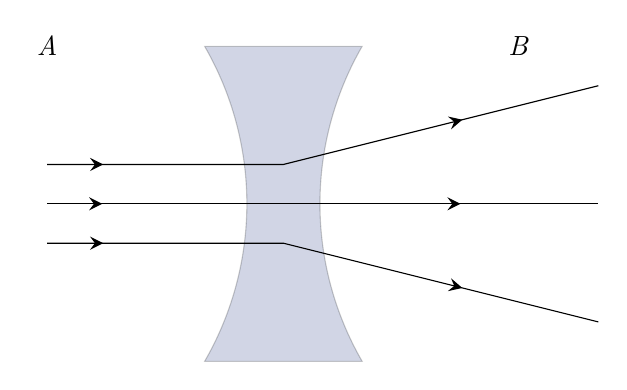
\begin{tikzpicture}[scale=2]
\pgfmathsetmacro{\lH}{1}
\pgfmathsetmacro{\lR}{2}
\pgfmathsetmacro{\sA}{asin(\lH/\lR)}
\pgfmathsetmacro{\base}{1}
\pgfmathsetmacro{\xshi}{\base/2}

\draw[yshift = -2cm, xshift = -\xshi cm,name path=lens, fill=mode1, opacity=0.2] (0, \lH cm)
arc[start angle = -\sA, delta angle = 2*\sA, radius = \lR cm] --
+(\base cm, 0)
arc[start angle = 180 - \sA, delta angle = 2*\sA, radius = \lR cm]
-- cycle;
\fill[fill = black] (-1cm, 0) coordinate (F) circle[radius = 0cm];

\begin{scope}[decoration = {
	markings,
	mark = at position 0.1 with {\arrow[scale=1.5]{stealth}},
	mark = at position 0.75 with {\arrow[scale=1.5]{stealth}}
}
]
\foreach \y  in {0.25, 0, -0.25}{
	\draw[postaction = decorate] (-1.5cm, \y cm) -- (0, \y cm)
	coordinate (A) 
	-- ($(F)!3!(A)$) ;      
	%extend lines along the path command here;
}
\end{scope}
\node at (-1.5cm,1) {\textit{A}};
\node at (1.5cm,1) {\textit{B}};
\end{tikzpicture}
		\caption{}
	\end{subfigure}%
	\begin{subfigure}{0.5\textwidth}
		\centering
		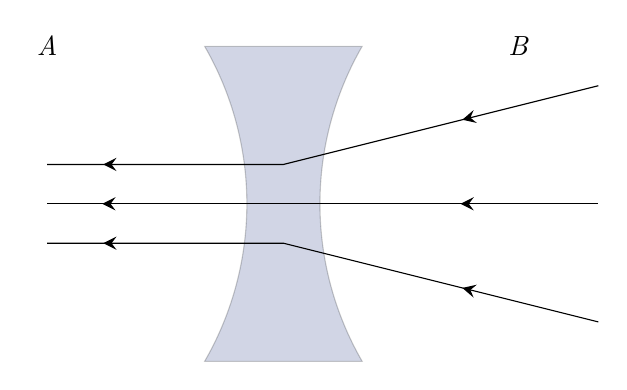
\begin{tikzpicture}[scale=2]
\pgfmathsetmacro{\lH}{1}
\pgfmathsetmacro{\lR}{2}
\pgfmathsetmacro{\sA}{asin(\lH/\lR)}
\pgfmathsetmacro{\base}{1}
\pgfmathsetmacro{\xshi}{\base/2}

\draw[yshift = -2cm, xshift = -\xshi cm,name path=lens, fill=mode1, opacity=0.2] (0, \lH cm)
arc[start angle = -\sA, delta angle = 2*\sA, radius = \lR cm] --
+(\base cm, 0)
arc[start angle = 180 - \sA, delta angle = 2*\sA, radius = \lR cm]
-- cycle;
\fill[fill = black] (-1cm, 0) coordinate (F) circle[radius = 0cm];

\begin{scope}[decoration = {
	markings,
	mark = at position 0.1 with {\arrow[rotate=180, scale = 1.5]{stealth}},
	mark = at position 0.75 with {\arrow[rotate=180, scale = 1.5]{stealth}}
}
]
\foreach \y  in {0.25, 0, -0.25}{
	\draw[postaction = decorate] (-1.5cm, \y cm) -- (0, \y cm)
	coordinate (A) 
	-- ($(F)!3!(A)$) ;      
	%extend lines along the path command here;
}
\end{scope}
\node at (-1.5cm,1) {\textit{A}};
\node at (1.5cm,1) {\textit{B}};
\end{tikzpicture}
		\caption{}
	\end{subfigure}%
	\caption[Time-reversed path in a double concave lens]{Reciprocity in a double concave lens for light rays travelling from \textbf{(a)} A to B, and \textbf{(b)} B to A. Since reciprocity holds for the system, light travelling along its time reversed path (B to A) will return back to its original state. This is true for \textit{any} scattering event, not just the divergence of rays through a lens.}
	\label{fig:reciprocity}
\end{figure}

In electromagnetism reciprocity is known under the guise of \textit{Lorentz reciprocity}, which mathematically expresses the idea of parity and time-reversal (PT) symmetry for an electromagnetic wave. In general terms, Lorentz reciprocity demands that if light can travel from some region \textit{A} to another region \textit{B}, then the reverse also holds (Fig \ref{fig:reciprocity}). Consider for example the random scattering of a laser in a medium. If it were possible to selectively take all the scattered wavelets and reverse their direction, then reciprocity would ensure that the they would recombine back into a coherent beam that emerges at the original angle of incidence \cite{Wiersma2013a}. In other words, if the propagation of a light wave were to be reversed then the properties of its transmission would remain unaffected \cite{Potton2004a}. It is evident that this is a direct consequence of the more generalised form of reciprocity as described above, as reciprocity requires that waves which propagate along time-reversed paths exhibit identical properties of transmission, regardless of how complicated such a path might be \cite{Buehler2016}.

Although reciprocal propagation of light is sometimes a desirable facet of optical devices, being able to dynamically constrain and manipulate the direction light can travel has tremendously useful applications, ranging from the reduction of noise in optical experiments \cite{Khanikaev2014a}, to exhibiting novel quantum effects of light \cite{Yilmaz2015a}. The most commonly employed method of breaking reciprocity in photonics is through the magnetic biasing of a system (where the magnetic field $\bm{B}$ is a pseudo-vector, making it odd under time-reversal \cite{Wang2006a}). In optics, magnetically biased techniques are crucial to the function of optical isolators, non-reciprocal devices that permit forward propagation of light while restricting counter-propagation \cite{Jalas2013a}, effectively constituting \textit{diodes} for light. Such commercially available isolators make use of the magneto-optic Faraday effect, where the plane of polarisation of a light source is rotated along the path of its trajectory. However, practical implementation of the Faraday effect in integrated photonics remains largely infeasible, owing to the incompatibility of binding magneto-optic materials to standard metal-oxide semiconductors \cite{Feng2011a} as well as the difficulty in scaling to optical frequencies \cite{Monticone2017}. Additionally, since the rotation of the plane of polarisation is dependent on the path length the light travels through, any optical device constructed with this approach must be large enough to accommodate a sufficient rotation. These restrictions impose a fundamental limit on both the size and potential applications of non-reciprocal devices that make use of a magneto-optic biasing. Despite this, there is good reason why magneto-optics has remained the de-facto standard of non-reciprocal devices; magneto-optically active materials are inexpensive, widely available, and simple to work with, making them attractive from an engineering standpoint in devices where size limitations are not strictly enforced.

Small-scale compatibility of non-reciprocal optics forms a primary hurdle in the realisation of fully-fledged photonic circuits. This has motivated a significant amount of interest in searching for alternative methods for inducing non-reciprocity without bulk magneto-optics \cite{Fang2012a, Rabla, Shoji2014,Li2014a}. Being able to isolate signals from one another is crucial to integrated photonics, which are currently hampered by significant noise and backscattering, leading to coherent interference in experiments and noise-sensitive designs. Nature however, provides startlingly few options to break reciprocity for light. As of yet there are only three known classes of techniques that are non-reciprocal. These includes the aforementioned magneto-optic biasing, non-linearities of materials, and the use of media that possess a \textit{time-dependence}.

\subsection{Relation to time-reversal symmetry}
In most literature, reciprocity and time-reversal symmetry are often used synonymously. Despite this being the case for a majority of reciprocal processes, there are several situations where a breaking of TR-symmetry does not imply a reciprocity violation. Lorentz reciprocity occurs when a wave satisfies a symmetry property that connects a scattering process with the reversed one. However, this is a generalisation of the principle of TR-symmetry, and the two are not always interchangeable in the realm of optics. This is because Lorentz reciprocity relates input and output waves in pairs, irrespective of the presence (or lack thereof) of other waves in the system. For optical systems reciprocity can be applied even when absorption in a material takes place - a process that is TR asymmetric, but still reciprocal \cite{Potton2004a}.

\section{Non-reciprocity in time-dependent systems}
\label{mome}

Consider a glass of water with light incident upon its surface. Now, assume that the water is dispersionless, and to a large degree incompressible. As the light passes through the water, it will gain an overall phase shift while its other properties will remain unchanged. But what if the water is then set into motion? It is found that the light develops an interference structure that is dependent on the velocity of the medium \cite{Zalesny2001a}. Even coherent light - lasers, will slightly bend in their trajectory whilst passing through the water. The amount of dragging the light experiences is directly proportional to the velocity and refractive index of the medium, a phenomenon that has been well known since Fizeau's experiment (1851) on the speed of light in water. Most importantly however, the symmetry of light transmission in the water is non-reciprocal: a slight phase shift is acquired when the light propagates with the water flow. On the other hand, light propagating in the reverse direction will acquire a negative phase shift. This idea of a medium that possesses some kind of time-dependent bias forms an important class of non-reciprocal devices. 

Lorentz reciprocity is derived on the grounds of time-independent media and time-harmonic fields \cite{Caloz2016}. It is apparent then that an optical medium that exhibits some kind of time-dependence can not be constrained by the reciprocity theorem. A moving medium will induce a non-reciprocal phase shift for light. This can be intuitively understood due to the flow vector $\bm{v}$ of the water being odd under time-reversal, akin to the pseudo-vector in magneto-optically active materials. The phase shifts obtained by the light are not directly observable. Similarly to how voltage can only be measured as a potential difference, the phase of light can only be measured relative to the phase of another electromagnetic wave. This measurement is exclusively made by examining the interference pattern of the light \cite{Tzuang2014a}.

\section{Outline}
This thesis will focus primarily on non-reciprocity in time-dependent media, and discuss how such non-reciprocal phases give rise to a synthetic gauge potential for light. The introduction of a gauge potential gives rise to a photonic analogue of the Aharonov-Bohm effect which is demonstrated through full-wave finite difference methods. 

In Chapter \ref{chapter:synthetic}, a review of recent developments in the field of synthetic gauge fields is presented. The review explores how non-reciprocal phases give rise to a photonic gauge field, and how suitable tailoring of the phases culminates in effective magnetic fields. These effective magnetic fields for light are vital in the nascent field of topological photonics. 

Chapter \ref{chapter:theory} presents a theoretical derivation of the effective gauge potential arising from a moving medium - and how such motion is equivalent to a modulation of the permittivity of a waveguide. It is then shown how a photonic analogue of the Aharonov-Bohm effect can be demonstrated with a rotating dielectric medium and a modulated waveguide. 

In Chapter \ref{chapter:method}, the finite-difference method for electromagnetic simulations is discussed and implemented for the purpose of demonstrating non-reciprocal phases in modulated waveguides. Both time and frequency domain simulations are considered.

Finally, in Chapter \ref{chapter:results}, non-reciprocal mode conversion is numerically validated and demonstrated, as well as a photonic Aharonov-Bohm effect for the purposes of optical isolation. Discussions of the feasibility of such devices is considered, and both implementations of numerical methods are then compared.
    \chapter[Review of synthetic gauge fields in photonics]{Review of synthetic gauge fields in photonics\footnote{This chapter is reproduced in part with permission, from Hey \& Li \textit{``Advances in Synthetic Gauge Fields through Dynamic Modulation"} 2017, submitted to \textit{Optics Communications} for publication.}}
\label{chapter:synthetic}
To achieve fine-control over light one may use so-called synthetic gauge fields. A synthetic gauge field is the tailoring of specific conditions such that some quantity of neutral particles emulates the dynamics of charged particles in a magnetic field. The rotation of a trapping of neutral atoms constitutes one such field: the Coriolis force, $F_C = -2 m \Omega \times \bm{v}$ couples to the atoms in a manner analogous to the classical Lorentz force, $F_L = q(\bm{v} \times \bm{B})$  \cite{Dalibard2015b}. Conversely, the mechanism for generating a synthetic gauge field for cold atoms relies on changing some internal degree of freedom to impart a phase to the wave function over time \cite{Dalibard2011b}. Similar synthetic gauge fields have also been explored in opto-mechanics \cite{Walter2016, Yang2017}  and acoustics \cite{Miri2017a,Yang2016b}. This lends itself to the question of whether it is possible to achieve similar conditions for light, and has motivated significant research into the field of synthetic gauge fields in photonics \cite{Fang2013b,Fan2015}. 

These synthetic gauge fields have proved instrumental in the nascent field of topological photonics, where a transfer of edifice from electronic systems has created a wealth of research ideas, ranging from the observation of protected edge states of light, where light moves along the edge of a system \cite{Wang2009b,Poshakinskiy2014,Rechtsman2013c,Raghu2008,Barik2016} to Floquet topological insulators, devices that are characterised by edge states immune to disorder \cite{Chen2014,Lumer2013,Zhang2015,Leykam2016,Maczewsky2016,Khanikaev2013}. In photonics, spatial periodicity of a lattice is combined with a synthetic gauge field, leading to 2D energy bands that are distinguished by the topological invariant known as the first Chern number. Suitable engineering of synthetic gauge fields thus has the potential to explore higher dimensional topologies, and the first experimental work on 3D lattices has unveiled particularly intriguing topological features, including the elusive Weyl points. Going further, recent work has begun on examining 4D topologically non-trivial effects of light \cite{Ozawa2016}.

\section{Inducing a photonic gauge field}

\label{sec:inducing}
Originally, the concept of generating a synthetic gauge field for photons was limited to a static ring resonator lattice that is carefully engineered to impart direction-dependent phases to photons with opposite spins \cite{Umucallar2011a}. On a single dielectric ring, light will resonate when it constructively interferes with itself after making a full round-trip \cite{Bogaerts2012}, in what are known as `whispering gallery' modes, so named for their acoustic origin in St Paul's cathedral where whispered sounds propagate along the circumference of the circular interior. In a periodic array of these resonators, it is possible for photons to `hop' between different rings, in a manner that is analogous to electrons tunnelling between atoms in a crystal. As a result, the edge modes of opposite spins propagate in opposite directions, realising a photonic analogue of the quantum spin Hall effect, a phenomena typically associated with electrons that is characterised by propagation only on the surface of a material. However, structures engineered in this way are susceptible to backscattering, since TR-symmetry is not broken. 


\begin{figure}[t]
	\centering
	\def\svgwidth{0.5\textwidth}
	\begin{normalsize}
		\input{figures/DynamicLattice.pdf_tex}
	\end{normalsize}
	\caption[A 2D dynamically modulated lattice of photonic resonators]{A 2D dynamically modulated lattice of photonic resonators, with two square sub-lattices of respective frequencies $\omega_A$ (red) and $\omega_B$ (blue). There is nearest neighbour coupling so that photons can only ‘hop’ between points via suitable modulation, acquiring a non-reciprocal phase. The phase on the horizontal bonds is $0$ (not shown), whereas the phase on the vertical bonds is linearly proportional to the column index, with a sign flip every 2nd index. This modulation choice corresponds to the Landau gauge. Image re-drawn from \cite{Fang2012}.}
	\label{fig:dynamiclattice}
\end{figure}
 
By applying a \textit{time-dependent} harmonic modulation to a photonic systems refractive index, it is possible to break this TR-symmetry and introduce a gauge field for light \cite{Fang2012}, as in Figure \ref{fig:dynamiclattice}. This process, known as dynamic modulation was first conceived by Fang et al. and later extended to a network of resonating lattices \cite{Fang2012a}. In applying the modulation, the phase of light becomes direction-dependent. This phase is strictly non-reciprocal, and consequently, possesses a broken TR-symmetry; reverting the direction of propagation will reverse the sign of phase. As far as the photon is concerned, the phase of some wave function cannot be directly measured, only differences in phase, and thus represents a gauge degree of freedom. This phase possesses the same gauge ambiguity as that of the phase acquired in an electronic gauge potential along an open path. Likewise, reverting the direction of propagation results in a change of sign. Consequently, this phase has the same properties as the electronic Aharonov-Bohm (AB) phase, so that demonstrating non-reciprocity is equivalent to showing the existence of a gauge potential for photons.  

\subsection{The electronic Aharonov-Bohm effect}

\begin{figure}[t]
	\centering
	\def\svgwidth{0.8\textwidth}
	\begin{normalsize}
		\input{figures/lasttest.pdf_tex}
	\end{normalsize}
	\caption[Aharonov-Bohm effect for charged particles]{The Aharonov-Bohm effect for electrons. An infinitely long solenoid has its magnetic flux confined entirely within its core. Surrounding the cylinder, the $\bm{B}$ field vanishes but the magnetic vector potential $\bm{A}$ remains. The potential causes the electrons to gain a negative or positive phase depending on their path through the potential.}
	\label{fig:abeffectfinal}
\end{figure}

Classically, for charged particles the AB effect is characterised by the acquisition of phase of a charged particle as it traverses a path-dependent potential where both the electric $\bm{E}$ and magnetic $\bm{B}$ fields vanish as in Figure \ref{fig:abeffectfinal} \cite{Aharonov1959}. The magnetic vector potential of the fields is non-vanishing in this region and mediates interactions with the magnetic field. In circulating around the potential, the electron acquires a positive or negative phase which can only be observed through interference of both paths. The Aharonov-Bohm effect demonstrates the importance of the gauge potential in quantum systems, and in fact is a prerequisite for the existence of such potentials \cite{Aharonov1959}. The AB effect has been widely demonstrated for electrons and other charged particles \cite{Chambers1960}, however it was only recently shown by Fang et al. (2013) that the gauge potential from non-reciprocal phases of light can be exploited to demonstrate an optical equivalent to the AB effect for light at radio frequencies \cite{Fang2013c}.
 

 \subsection{An effective magnetic field for light}
 Non-reciprocal phases of light in time-varying systems have been shown to give rise to an important phenomenon - effective magnetic fields for light. Fang et al (2012) first demonstrated that an effective magnetic field for light can arise if the phase of the light were non-reciprocal \cite{Fang2012a}. The effective magnetic field is directly linked to the idea of a gauge potential, similar to how the classical electromagnetic field $\bm{B}$ arises from the magnetic vector potential $\bm{A}$. In fact, the non-reciprocal phase shift acquired by light in a moving medium discussed in the beginning of section \ref{mome} satisfies the requirements for generating a gauge potential. This is incredibly useful from an optical standpoint, as photons, being neutral particles, do not naturally couple to magnetic fields.
 
 Fang et al. later went on to demonstrate that such effective magnetic fields can arise from the aforementioned dynamic modulation of a ring resonator lattice \cite{Fang2013}. By imposing a specific arrangement of non-reciprocal phases for light in the structure, the resulting arrangement corresponds to a uniform magnetic field for light. Despite acknowledging the possibility of the harmonic modulation to give rise to any kind of directed effective field, Fang et al. only simulated a uniform field causing the light to move in circular motion. Additionally, practical creation of a lattice with the required levels of finesse are noted to be highly difficult from an engineering standpoint.
 
 Other non-reciprocal phase induced fields also consider an array of resonators that impose a static direction dependent phase \cite{Haldane2008b}. However, all of these suffer from a similar flaw - practical implementation of the resonators is incredibly difficult, and the final system is static in nature, in contrast to dynamically modulated systems. It has been noted by Lin and Fan (2015) that the resonators themselves provide no essential role with respect to the effective field generated, beyond simplifying the theoretical treatment \cite{Lin2015a}. As a result, they have derived a 'resonator-free' system that is based instead on a purely two-dimensional network of waveguides.  
 
 Resonators and waveguides are not the only methods of inducing a non-reciprocal phase (and consequently, a gauge potential for light). Li et al. (2014) demonstrated that photon-phonon interactions within acousto-optic crystals introduces a non-reciprocal phase for light \cite{Li2014a}. From this, they demonstrated an optical Aharonov-Bohm effect at visible frequencies, one the first of such kind observed through non-reciprocal phases. The possibility of realising an effective magnetic field for photons gives rise to an important number of effects that are similar to phenomena exhibited by electrons in a magnetic fields, such as a Lorentz force \cite{Fang2012}, quantum Hall effects, and topologically protected one-way edge modes \cite{Fang2013}. While some of these effects have been noted to be possible with magneto-optics \cite{Wang2009, Lee2017a}, dynamic modulation is both more versatile and offers a greater coupling strength at optical frequencies.
 
 \subsection{Fluid moving media}
 
 The idea of exploiting non-reciprocal phase shifts to demonstrate an AB effect has been naturally extended to the simpler cases of light in moving media. Vieira et al (2014) discussed an implementation for inducing non-reciprocal phases in light by submerging a rotating cylinder in a viscous medium. The rotation of the cylinder imparts an angular \textit{biasing} to the medium, which creates a non-reciprocal phase for the light by mediating interactions between the cylinder and light in a manner similar to how the magnetic vector potential mediates interactions with the magnetic field \cite{Vieira2014a}. In this method, the effective magnetic field for the light is given by the vorticity (the local rotation of the vector field) of the medium in which it is present, again similar to how the magnetic field is the curl (or vorticity) of the magnetic potential. 
 
 Vieira's result is not the first for wavelike phenomena in rotating media. It has previously been shown by de Rosny et al. (2005) that a rotational flow can break the reciprocal transmission of ultrasound waves, along with Leonhardt's \cite{Leonhardt1999, Leonhardt2000c, Leonhardt2000a} pioneering formulations of the effective gauge potentials for light. In Leonhardt's work, not only was a possible AB effect suggested, but it was also shown that a medium with high enough viscosity and refractive index can bend and trap light similarly to a black hole, a result that has been subsequently proven in multiple experiments \cite{Genov2011}.
 
\section{Topological photonics \label{topology}}
\label{sec:topology}

Dynamically modulated resonator lattices also support one-way propagation along the edges (edge modes). However, time-harmonic modulations of more than a few resonators simultaneously is a challenging feat at optical wavelengths \cite{Tzuang2014}. Rechtsman et al. (2013) showed that it is possible to shift the modulation from the frequency to the spatial domain to observe photonic analogues of the quantum Hall effect at optical frequencies \cite{Rechtsman2013b}, corresponding to the first experimentally viable Floquet topological insulators \cite{Lindner2011}. Instead of breaking TR-symmetry in their system, the authors instead broke spatial symmetry along the $z$-axis, and identified their system as being suitably analogous to a breaking of TR-symmetry, culminating in protected edge modes. 

Most previous works have focused solely on the regime where the modulation strength is far less than the modulation frequency \cite{Lee2017a}, allowing for the application of the rotating-wave approximation (RWA), where slowly varying terms are ignored. On the other hand, there has been recent interest in light-matter interactions in the ultra-strong coupling regime \cite{Fedortchenko2016,Hirokawa2017}, where the RWA is no longer valid. In such ultra-strong coupling systems, it has been shown that topologically protected one-way edge states in dynamic modulation are less susceptible to intrinsic losses \cite{Fan2015}. In addition to this, a unique topological phase transition was found to be associated with variations in the modulation strength \cite{Yuan2015a}. Such phase transitions are not found in rotating-wave counterparts. 

\subsection{Synthetic dimensions}

Studies in topology have long hinted at rich possibilities of physics in higher dimensions, namely analogues of the quantum Hall effect in even-dimensional spaces \cite{Zhang2001}. Traditional systems in condensed matter physics however, are locked out of examining such effects. Only recently have new approaches in simulating higher dimensional topological models, so-called ‘synthetic dimensions’ have been proposed, that generate a gauge field for neutral particles by exploiting additional degrees of freedom \cite{Price2017,Saito2017,Barbarino2016}. These ideas were first proposed in ultra-cold atomic gases\cite{Stuhl2015a,Boada2012}, where the atoms possess an internal spin degree of freedom. Photons naturally possess many internal degrees of freedom: frequency, orbital angular momentum, spin angular momentum, polarization, and so on. These additional degrees of freedom can form synthetic lattice dimensions for light, leading to possible experimental analysis of higher dimensional topological photonics. Due to the long-range interactions of light in synthetic dimensions however, there is a difficulty associated with exploring quantum Hall effects \cite{acki2016,Zeng2015}.
  
Here, a basic method of achieving synthetic dimensions via dynamic modulation is demonstrated. Consider one of the most elementary photonic structures - the ubiquitous ring resonator. In the absence of group velocity dispersion (where the group velocity depends on the wavelength), the single ring supports a set of equally spaced resonant frequencies. The spacing of the modes $\Omega$ is based on the spectral range of the resonator, and is related to the round-trip time $T$ by $\Omega =  2 \pi /T$.

\begin{figure}[t]
	\centering
	\def\svgwidth{0.5\textwidth}
	\begin{normalsize}
		\input{figures/1DSynthetic.pdf_tex}
	\end{normalsize}
	\caption[Modulated ring resonator with a synthetic dimension]{A ring resonator undergoing dynamic modulation of frequency $\Omega_M$, which supports several equally spaced resonant modes. The resonator modes form a synthetic dimension along the frequency axis, and by transitioning the light between different frequencies, it is possible to examine \textit{1D} physics on the \textit{0D} ring structure. Although the light is propagating effectively in $3D$ in the ring, the single mode can be considered to be point-like $0D$.}
	\label{fig:syntheticring}
\end{figure} 

By dynamically modulating the ring structure, as in Figure \ref{fig:syntheticring}, modes on the ring undergo transitions to higher order sidebands, separated by the modulation frequency $\Omega_M$. If the modulation frequency is then chosen to be equal to the mode spacing of the resonator $\Omega$, there will be a resonant coupling of the modes that are separated by the free-spectral range of the ring (the frequency spacing naturally supported by the ring). Consequently, this system can be described by a \textit{1D} tight-binding model, despite being a \textit{0D} structure, as the spacing of the frequencies represent an additional degree of freedom for the light. This can naturally be extended to the case of a $1D$ array of ring resonators that are coupled together to form a waveguide \cite{Yuan2016c}. Each ring has a controlled phase of modulation, which gives rise to \textit{2D} physics model on a $1D$ structure. The phase of the modulation corresponds then to the hopping phase along the frequency axis.

It is possible to generate a topologically non-trivial bulk correspondence by considering boundaries in real and synthetic space. In real space, the boundary is given by the physical edges of the ring. However, in frequency space, a boundary is introduced by the group velocity dispersion (GVD) of the ring instead (how the ring affects the duration of optical pulses propagating within it). Around the zero-GVD point, most frequencies are equally spaced so the modulators induce an on-resonance coupling. On the other hand, away from the zero-GVD point, the frequencies are no longer equally spaced and thus cannot support coupling, leading to an effective \textit{boundary} in frequency space. Thus, light propagating along the system will encounter a boundary composed of the real physical size of the rings in combination with the GVD. Finally, we note that outside of applications in topological photonics discussed below, synthetic dimensions in dynamic modulation have also recently been shown to support efficient frequency manipulation of light \cite{Qin2017}.

\subsection{Weyl points}

\begin{figure}[t]
\centering
\def\svgwidth{0.8\textwidth}
\begin{normalsize}
\input{figures/3DDynamicMod.pdf_tex}
\end{normalsize}
\caption[A $3D$ synthetic resonator lattice]{An example resonator structure for examining 4D topological photonics. Dynamic coupling between rings allows for $3D$ propagation. The supported frequencies of the resonators, $\omega$, as usual provide the synthetic dimension allowing for the possibility of examining $4D$ topological physics with light.}
\label{fig:synthetic3d}
\end{figure}

In condensed matter systems, the Weyl point describes a magnetic monopole in momentum space, that is, a `source' or `sink' of Berry curvature. As such, the Weyl point is perceived as topological nodal points in 3D momentum space. Weyl points are topologically robust, in the sense that they cannot be destroyed by any perturbation that preserves translational symmetry. The Hamiltonian of a Weyl system is
$H=k_x \sigma_x+k_y \sigma_y+k_z \sigma_z+E_0 I$
where $\sigma_{x,y,z}$ are the Pauli spin matrices, and $I$ is the \textit{2x2} identity matrix, which together form a complete basis for \textit{2x2} Hermitian matrices. There has been a massive effort devoted to investigating Weyl points and their associated phenomena in electronic systems \cite{Gupta2017,Spivak2016}, and have also been found in photonic crystals \cite{Noh2017,Xiao2016}, as well as acoustic \cite{Yang2016a} and plasmonic structures \cite{Gao2016}. 

To explore a Weyl point in a planar \textit{2D} geometry, one may use a synthetic dimension to simulate the third spatial dimension, by again considering arrays of ring resonators – this time arranged in a honeycomb lattice. The size of the synthetic dimension, which corresponds to the number of modes in each individual ring can be chosen to be almost arbitrarily large without increasing the system complexity. In a recent paper, Lin et al suggested that it is possible to investigate a synthetic 3D space through dynamic modulation of \textit{2D} on-chip ring resonators \cite{Lin2017}. Each resonator supports a set of discrete modes equally spaced in resonant frequency. The synthetic dimension then originates from these discrete modes, manifesting as a synthetic periodic lattice so that the entire system can be envisaged as a 3D space. This on-chip dynamic modulation is readily feasible, as compared with previous complex electromagnetic or acoustic structures for realizing Weyl points \cite{Lu2015,Rechtsman2013}, a planar 2D approach is more flexible owing to the dynamic nature of the system, and can be achieved with the previously discussed extension of dynamic modulation in synthetic dimensions, allowing for on-chip investigation of Weyl points. 

\subsection{Towards 4D photonics}
Naturally, the quantum Hall effect was first generalized to higher dimensions for electronic systems \cite{Zhang2001}. It is a standard extension of our discussion on 3D photonic systems to then consider a 3D array of resonators in the three spatial dimensions $x$, $y$, $z$ and then extending into the synthetic frequency dimensions $\omega$ to probe elusive 4D quantum Hall effects.

A 4-dimensional model making use of 3D resonating lattices with plaquettes has only recently been proposed by Price et al., based on the authors previous works in 4D quantum Hall effects for ultra-cold atoms \cite{Price2015}. This model differs to a potential synthetic dimension with dynamic modulation in Figure \ref{fig:synthetic3d}, as their lattice model does not break TR-symmetry. Because of this, photons with positive angular momentum can backscatter into states with a negative angular momentum. However, it has been noted that such backscattering can be minimised during fabrication \cite{Hafezi2013a}. Finally, we note that achieving a 4D topological effect for light would not only be possible under a dynamic modulation regime, but also would involve a broken TR-symmetry, leading to one-way edge modes propagating on the boundaries of a 3D frequency space.

    \chapter{Gauge potentials in time-dependent media}
\label{chapter:theory}

From the previous chapter, the generation of a synthetic gauge \textit{field} relies completely on the presence of a synthetic gauge \textit{potential} which arises from the existence of non-reciprocal phases. Creating these phases for light invariably requires breaking reciprocity. Here, it is shown that the influence of the velocity field on light in a moving medium can be formulated in terms of a gauge potential, which will lead to observable measurements of a direction-dependent phase. The more constrained case of a potential arising from the motion of water in both a linear waveguide and surrounding a rotating cylinder dielectric will then be shown to act as an effective magnetic potential for light, introducing a non-reciprocal phase that can be exploited to demonstrate an optical analogue to the Aharonov-Bohm effect. This phase can also be generated through dynamic modulation of a waveguide, and the gauge potential emerging from such modulations is derived based on the work of Fang et al. \cite{Fang2012}.

\section{Moving media}

To show how a moving media forms an effective vector potential for light, first consider the curl components of Maxwell's equations for moving media without sources \cite{Mansuripur2009a},

\begin{align} 
	\nabla \times \bm{E} &= -\dfrac{\partial \bm{B}}{\partial t}, \label{mwell3}\\
	\nabla \times \bm{H} &= \dfrac{\partial \bm{D}}{\partial t} \label{mwell4}.
\end{align}

Let $\bm{v(r)}$ represent the velocity field associated with the motion of a medium of refractive index $n$, moving along $v \hat{x}$. Then, by taking a first order approximation of the Minkowski relations \ref{HMinkowski} and \ref{DMinkowski}, where $\textbf{v}/c \ll 1$,

\begin{align}
	\bm{B} &= \mu \bm{H} - (n^2 - 1) \dfrac{\bm{v}}{c^2} \times \bm{E}, \\
	\bm{D} &= \epsilon \bm{E} + (n^2 - 1) \dfrac{\bm{v}}{c^2} \times \bm{H}.
\end{align}

These relations allow us to rewrite the curl components of Maxwell's equations in the form

\begin{align}
\nabla \times \bm{E}  -\dfrac{\partial}{\partial t} \Big[(n^2 - 1) \dfrac{\bm{v}}{c^2} \times \bm{E}\Big] &=-\dfrac{\partial}{\partial t}(\mu\bm{H}), \label{a2}\\
\nabla \times \bm{H}  -\dfrac{\partial}{\partial t} \Big[(n^2 - 1) \dfrac{\bm{v}}{c^2} \times \bm{H}\Big] &=-\dfrac{\partial}{\partial t}(\epsilon\bm{E}). \label{a1}
\end{align}

To solve these equations explicitly, we shall assume the light in the media to be a monochromatic plane wave with electric and magnetic fields defined as 

\begin{equation}
\begin{bmatrix}
\bm{E}(\bm{r},t) \\
\bm{H}(\bm{r},t)
\end{bmatrix}
=
\begin{bmatrix}
\bm{E}(\bm{r}) \\
\bm{H}(\bm{r}) 
\end{bmatrix}
e^{-i \omega t},
\label{eqn:planewave}
\end{equation}

which simplifies equations \ref{a2} and \ref{a1} to

\begin{equation}
\Big(\nabla + i \omega (n^2 - 1) \dfrac{\boldsymbol{v}}{c^2}\Big) \times 
\begin{bmatrix}
\bm{E} \\
\bm{H}
\end{bmatrix}
=
i\omega
\begin{bmatrix}
\mu \bm{H} \\
-\epsilon \bm{E}
\end{bmatrix}.
\label{a3}
\end{equation}

To elucidate the relationship between the quantum and classical approach used here, Equation \ref{a3} is multiplied by $-i \hbar$, where $\hbar$ is Planck's reduced constant to obtain

\begin{equation}
(\hat{p} + q \bm{v} ) \times 
\begin{bmatrix}
\bm{E} \\
\bm{H}
\end{bmatrix} 
= 
\hbar \omega
\begin{bmatrix}
\mu \bm{H} \\
-\epsilon \bm{E}
\end{bmatrix} .
\label{eqn:finalfield}
\end{equation}

Straight-away, the quantum momentum operator can be identified: $\hat{p} = -i \hbar \nabla$, as well as the effective charge for the photon in the medium,

\begin{equation}
q =\dfrac{\hbar \omega}{c^2}  (n^2 - 1).
\label{effectiveCharge}
\end{equation}

This charge, $q$, forms the \textit{effective} charge for the light in the medium. Furthermore, the relationship between the gauge potential $\bm{A}$ and flow vector $\bm{v}$ of the medium as simply

\begin{equation}
\bm{A(r)} = \bm{v(r)}.
\end{equation}

This result shows that a relative movement introduced in a medium can be formulated in terms of an effective vector potential, along with an associated `charge' for the light in the medium. 

\subsection{Non-reciprocal phase from a Fizeau-like apparatus}

\begin{figure}[t]
	\centering
	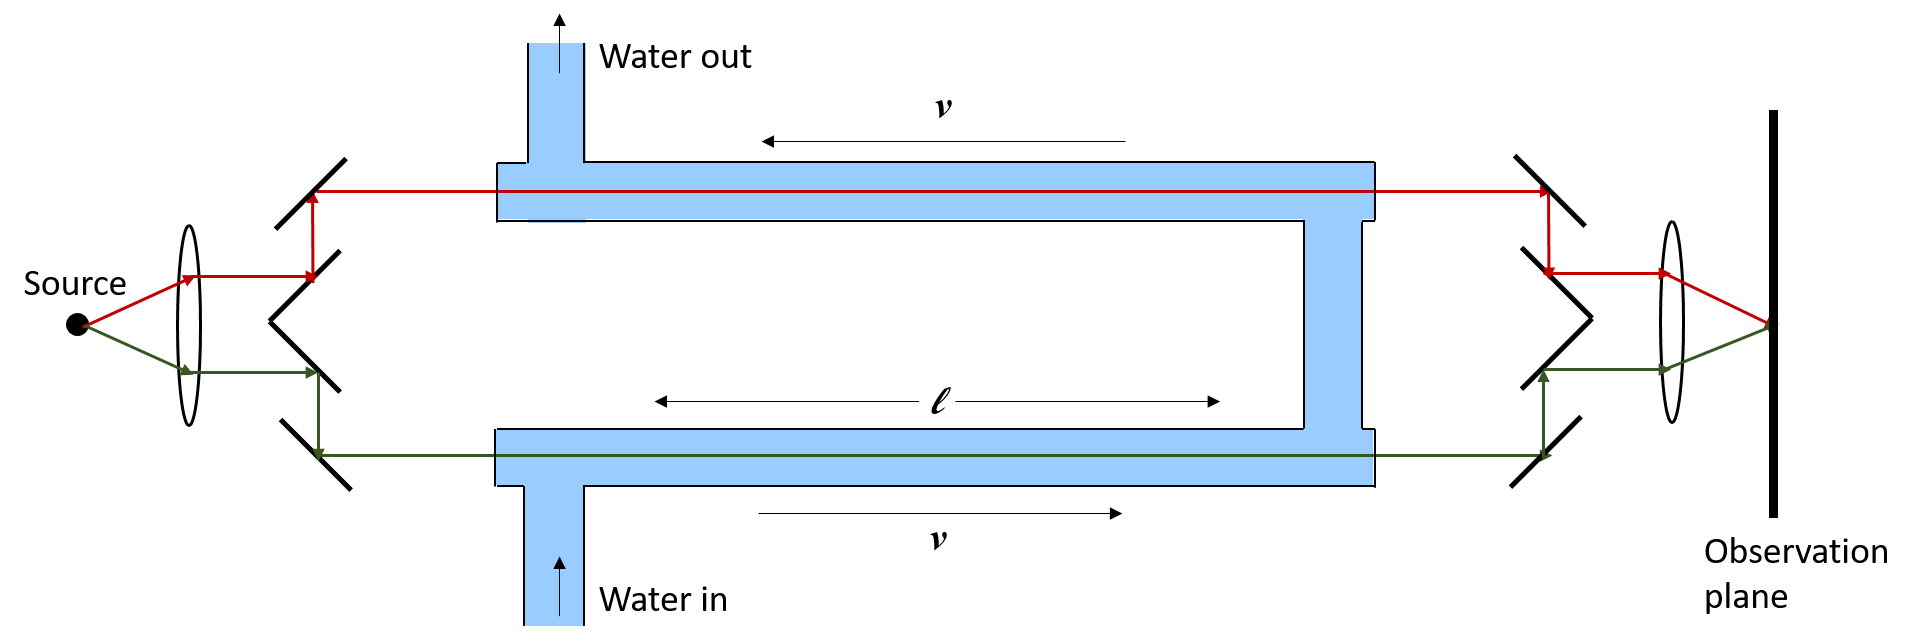
\includegraphics[width=\textwidth]{figures/fizeau.png}
	\caption[The standard apparatus for the Fizeau experiment]{A traditional form of the Fizeau experiment. A source of light is split into two beams, propagating with and against the flow vector of the water respectively. The dragging of the light by the medium forms a non-reciprocal phase, which can be observed by the resulting interference pattern.}
	\label{fig:fizeau}
\end{figure}


Now, consider what happens if a photon were to flow through a medium moving with a linear velocity along $x$, as depicted in Figure \ref{fig:fizeau}. To derive the phase shift it will gain, we will begin with Maxwell's equations from \ref{mwell3} to \ref{mwell4}. Rearranging the magnetic field intensity and displacement field, yields

\begin{align}
\nabla \times \bm{E} &= -\dfrac{\partial \bm{B}}{\partial t}, \label{mwell2_3}\\
\nabla \times \bm{B} &= \mu \epsilon \dfrac{\partial \bm{E}}{\partial t}.
\end{align}

Taking the curl of \ref{mwell2_3} yields,

\begin{equation}
\nabla \times (\nabla \times \bm{E}) = \nabla \times (-\dfrac{\partial \bm{B}}{\partial t}) = -\dfrac{\partial}{\partial t}(\epsilon \mu \dfrac{\partial \bm{E}}{\partial t}),
\end{equation}

where the divergence of the $\bm{E}$ field is $0$, reducing the above equations to the three dimensional Cartesian form of the electromagnetic wave equation,

\begin{equation}
\label{3dwave}
\big(\dfrac{n^2}{c^2} \nabla ^2 - \dfrac{\partial{^2}}{dt^2}\big)\bm{E} = 0.
\end{equation}

Equation \ref{3dwave} transforms under the appropriate Lorentz boost along $v\hat{x}$, defined in Appendix \ref{lorentz} as

\begin{equation}
\Big[1-\big(\dfrac{nv}{c}\big)^2 \Big] \nabla ^2 \bm{E} - \dfrac{2}{c^2} (n^2 - 1) \bm{v} \cdot \nabla \dfrac{\partial E}{\partial t} + \Big[\dfrac{v^2-(nc)^2}{c^4} \Big] \dfrac{\partial ^2 E}{\partial t^2} = 0.
\end{equation}

When the medium is moving slowly with respect to $c$ we can assume $v/c \ll 1$, then the above equation further reduces to the more manageable form

\begin{equation}
\label{boost3dwave}
\nabla ^2 \bm{E} - \dfrac{2}{c^2} (n^2 - 1) \bm{v} \cdot \nabla \dfrac{\partial E}{\partial t} - \dfrac{n^2}{c^2} \dfrac{\partial ^2 \bm{E}}{\partial t^2} = 0.
\end{equation}

Again assuming a monochromatic plane wave solution (\ref{eqn:planewave}) Equation \ref{boost3dwave} reduces to

\begin{equation}
\label{wavey}
\nabla ^2 E - 2i\dfrac{w^2}{c^2}(n^2-1)\dfrac{\bm{v}}{c} \cdot \nabla E + (n\dfrac{w}{c})^2 E = 0.
\end{equation}

Now, recall the time-independent Schr\"odinger equation for an electron in some potential $\bm{A(r)}$ \cite{Sakurai1995},

\begin{equation}
\dfrac{1}{2m} \Big(\dfrac{h}{i} \nabla - \dfrac{e}{c} \bm{A} \Big)^2 \psi = E \psi
\end{equation}

which can be expanded out to give

\begin{equation}
\label{schrod}
\nabla^2 \psi - \dfrac{ie}{\hbar c} \big[ \bm{A} \cdot \nabla \psi + (\nabla \cdot \bm{A}) \psi \big] + \big(\dfrac{2mE}{\hbar^2} + \dfrac{e^2}{\hbar^2 c^2} \bm{A}^2 \big) \psi = 0.
\end{equation}

By visual inspection alone, it is evident that equations \ref{schrod} and \ref{wavey} share a similar form in the low velocity regime to the first order, identical to our result in the previous section. To show this, consider the mapping of \ref{schrod} to the following relations; $\psi \rightarrow E$, $\bm{A} \rightarrow \bm{v}/c$, $e/\hbar c \rightarrow k(n^2-1)$, and $2mE/\hbar^2 \rightarrow (nk)^2$, from which

\begin{equation}
\nabla^2 E - ik(n^2-1) \big[ \dfrac{v}{c} \cdot \nabla E + (\nabla \cdot \dfrac{v}{c})E \big] + \big(n^2k^2 + (k(n^2-1))^2 \dfrac{v}{c} \big) E = 0.
\end{equation}

Which, in the first order approximation of $\textbf{v}/c$ becomes Equation \ref{wavey}. Now, the known solution of the above expanded Schr\"odinger solution is simply
\begin{equation}
\psi(\bm{r}) = \psi_0 \exp \Big[\dfrac{ie}{\hbar} \int_{}^{s(\bm{r})} \bm{A(r')} \cdot d\bm{s'} \Big],
\end{equation}
for a line integral over any path such that the final point $s(\bm{r}) = \bm{r}$ and the curl of $\bm{A}$ is vanishing. 

The interference between two phases traversing different paths is then
\begin{equation}
\Delta \varphi = \dfrac{q}{\hbar} \Big(\int_{P_1} \bm{A} \cdot d\bm{s} - \int_{P_2} \bm{A} \cdot d\bm{s} \Big),
\end{equation}

whereby application of Stoke's theorem,

\begin{equation}
\Delta \varphi = \dfrac{q}{\hbar} \int \nabla \times \bm{A} \cdot \hat{n}\textbf{dS},
\end{equation}

which is the quantum AB effect for electrons. It is evident that this is also a solution for the interference of \ref{wavey}, where the electromagnetic vector potential $\bm{A}$ is replaced with $\bm{v}$,

\begin{equation}
\varphi = \dfrac{w}{c^2} (n^2-1) \int_{S}^{} \nabla \times \bm{v} \cdot d\bm{S}.
\end{equation}
 
If the velocity of the medium in both arms of the Fizeau apparatus is assumed to be uniform, then we can assume $\nabla \times \bm{v} = 0$ for both propagation paths of length $l$. In this case the interference term becomes

%\varphi &= \dfrac{\omega}{c^2} \int_{}^{} 0 \cdot \hat{n} dr \\
\begin{equation}
\varphi = \dfrac{\omega}{c^2} (n^2-1) (2 v l).
\end{equation}

Thus we see that not only does a moving media form a synthetic gauge potential for photons, but that such a potential imparts \textit{direction dependent} phases on the light in question.

\subsection{Photonic Aharonov-Bohm effect for a rotating dielectric}

The potential is not constrained to exist only for linear motion. Here, it is shown that the rotation of a medium is sufficient to mimic the Aharonov-Bohm effect for light. The rotation of the medium forms an effective field that is synonymous with the rotation of the magnetic vector potential. In fact, the curl of the rotation itself gives rise to a gauge field, exactly how the magnetic field is the manifestation of the curl of the magnetic potential ($\bm{B} = \nabla \times \bm{A}$).

Consider first a dielectric cylinder of radius $R$, rotating with an angular velocity $\Omega \hat{z}$ while submerged in a uniform medium of constant viscosity as in Figure \ref{fig:abvieira}. Light traversing the medium will be shown to attain a non-reciprocal phase that is dependent on the radius and angular velocity of the dielectric, despite no interactions with the dielectric taking place. In the Aharonov-Bohm effect, the potential mediates interactions with the field. Here, the rotation of the medium instead mediates interactions with the dielectric cylinder \cite{Vieira2014a}.

\begin{figure}[t]
	\centering
	\def\svgwidth{0.6\textwidth}
	\begin{normalsize}
		\input{figures/RotatingCylinder.pdf_tex}
	\end{normalsize}
	\caption[A rotating medium analogue of the Aharonov-Bohm effect for light]{Proposed rotating cylinder for demonstrating an optical AB effect. A beam of photons is split into 2 paths, $P_1$ and $P_2$ of radius $b$, propagating around a rotating cylinder of angular frequency $\Omega$ immersed in a viscous medium. The light acquires a positive or negative phase depending on whether it is propagating with or against the rotation, leading to an optical AB phase.}
	\label{fig:abvieira}
\end{figure}

The angular velocity imparted to the medium is proportional to the distance from the cylinder. In cylindrical coordinates ($r, \theta, z$) the velocity of the cylinder and the surrounding medium is separated into two regions. One, for the inside of the cylinder ($0\leq r \leq R$), and another for the medium surrounding the cylinder ($r>R$).

\begin{equation}
\bm{v}(r) = 
\begin{cases}
\Omega r \hat{\theta}, & 0\leq r \leq R  \\
\dfrac{\Omega R^2}{r} \hat{\theta}, & r > R.
\end{cases}
\end{equation}

As such, there are two effective potentials dependent on the rotation of the cylinder. The effective field that the photon `feels' is then	

\begin{equation}
\bm{H} = \nabla \times \bm{v} = 
\begin{cases}
\Omega \hat{z}, & 0\leq r \leq R  \\
0, & r > R.
\end{cases}
\end{equation}

As expected, the effective field $\bm{H}$ is only non-vanishing inside the cylinder. Likewise, similar to electromagnetic fields, a vanishing of the magnetic field does not imply that the potential is also $0$. In fact, the vector potential is not uniquely defined, since any number of arbitrary curl-free components can be added without changing the effective field. As long as the cylinder is rotating at a constant angular velocity, the strength of the effective field as `felt' by the photon is independent of the position inside the cylinder.

Now, consider a light source propagating through the uniform medium surrounding the cylinder with respect to an observer in the rest frame (Fig \ref{fig:abvieira}. Surrounding the rotating cylinder, it has been shown that despite the effective magnetic field vanishing, an effective gauge potential of $\frac{\Omega R^2}{r} \hat{\theta}$ remains. Suppose that the packet of light is split into two separate paths of radius $b$, with path 2 ($P_1$) propagating in the direction of rotation, and path 1 ($P_2$) propagating along the opposite direction. In propagating along these paths, the wave-function of the light acquires a phase,

\begin{equation}
\phi_{1,2} = \dfrac{q}{\hbar} \int_{P_{1,2}}^{} \boldsymbol{A} \cdot d\boldsymbol{r}.
\end{equation}

So that the relative phase shift of the light along the paths $P_1$ and $P_2$, which both share the same initial and final points, is given by

\begin{equation}
\Delta \phi = \dfrac{q}{\hbar} \int_{P_1}^{} \boldsymbol{A} \cdot d\boldsymbol{r} - \dfrac{q}{\hbar} \int_{P_2}^{} \boldsymbol{A} \cdot d\boldsymbol{r} = \dfrac{q}{\hbar} \oint  \boldsymbol{A} \cdot d\boldsymbol{r}.
\end{equation}

An important distinction to make in the above equations is that they are independent of the time taken to traverse the closed path. In other words, a photon moving at close to the speed of light will acquire exactly the same phase as a photon travelling significantly slower.
Upon substitution of appropriate quantities, where $q$ is the effective charge of the photon derived in Equation \ref{effectiveCharge},

\begin{equation}
\phi = \dfrac{\omega}{c^2}(n^2 - 1) \int_{0}^{2\pi} \frac{\Omega R^2}{b} \hat{\theta} \cdot b d\theta \hat{\theta}.
\end{equation}

Explicitly calculating this phase difference yields the result

\begin{equation}
\phi = \dfrac{2 \pi \omega}{c^2} (n^2 - 1) \Omega R^2,
\end{equation}

where $n$ is the refractive index of the medium. That is, the phase difference of the interfering light is dependent on several properties of the dielectric cylinder. This result is exceedingly similar to the result for the linearly moving medium. The water still plays the same role as that of an effective potential, however the vorticity is no longer vanishing, and represents instead the effective field of the medium.

It is important to reiterate that both these processes are strictly non-reciprocal. Consider instead injecting photons from the right-hand side and measuring interference at the left. The photons previously propagating along the direction of rotation will now be circulating opposite to the media, and gain a negative phase shift. The phases of the light $\phi_1$ and $\phi_2$ impose a gauge potential for the photons. For a single photon, the phase of a single electromagnetic wave is not observable, representing a gauge degree of freedom. The phase obtained from the line integral of the gauge potential in the electronic AB effect has the same ambiguity. The phase difference between two paths however, is a detectable quantity through interferometry. Moreover, reverting the direction of propagation of the photons results in the change of the sign of the phase difference. Because of this, demonstrating the non-reciprocal phase is equivalent to a demonstration of the gauge potential for photons. 

\section{Dynamically modulated photonic structures}

\label{sec:modulation}
The question of dynamic media is subtle - what truly constitutes motion? The movement of a dielectric medium is an obvious one, but perhaps more subtle is the modulation of the refractive index of a medium in which light is propagating. As far as a photon is concerned, a moving medium is nothing more than a region of space in which the refractive index is time-dependent. In materials of unity permeability, the refractive index is simply $n=\sqrt{\epsilon}$. Thus, by applying a time-dependent change to the permittivity of a photonic structure, the refractive index also becomes time-dependent.

All photonic structures possess a dispersion relation, which is a collection of wavevectors $k$ and frequencies $\omega$ of allowed solutions to Maxwell's equations for a given set of boundary conditions. The dispersion relation dictates which \textit{modes} of light are allowed to propagate, and are separated into their component transverse electric $TE$ and transverse magnetic $TM$. Here, only $TE$ modes are considered, so that the first two bands on the dispersion relation are the $TE_0$ even and $TE_1$ odd modes as seen in Figure \ref{fig:bandsample}. Modes that exist below the light cone of $\omega = c k$ are known as guided, whereas those in the light cone are `radiation' or `leaky' modes, so named for the exponential loss of the electric field of the mode as it propagates in the waveguide.


\begin{figure}[t]
	\centering
	\setlength{\figH}{\textwidth}
	\setlength{\figW}{\textwidth}
	% This file was created by matlab2tikz.
%
%The latest updates can be retrieved from
%  http://www.mathworks.com/matlabcentral/fileexchange/22022-matlab2tikz-matlab2tikz
%where you can also make suggestions and rate matlab2tikz.
%
%
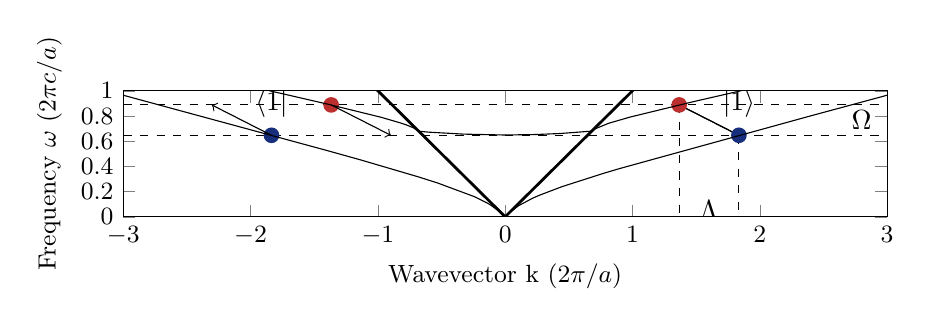
\begin{tikzpicture}

\begin{axis}[%
width=0.8\figW,
height=0.4\figH,
at={(0\figW,0\figH)},
scale only axis,
xmin=-3,
xmax=3,
xlabel={Wavevector k ($2\pi/a$)},
ylabel={Frequency $\omega$ ($2\pi c/a$)},
ymin=0,
ymax=1,
axis background/.style={fill=white}
]
\draw[dashed] (-3,0.6468) -- (3,0.6468);
\draw[dashed] (-3,0.8879) -- (3,0.8879);
\node at (2.8,0.767) {$\Omega$};
\draw[dashed] (1.836,0.6468) -- (1.836,0);
\draw[dashed] (1.367,0.8879) -- (1.367,0);
\node at (1.6,0.05) {$\Lambda$};
\draw[->] (1.836,0.6468) -- (1.367,0.8879);
\draw[->] (1.367,0.8879) -- (1.836,0.6468);
\node[label={90:{$\bra{1}$}},circle,fill=mode1,inner sep=2pt] at (-1.836,0.6468) {};
\node[label={90:{$\ket{1}$}},circle,fill=mode1,inner sep=2pt] at (1.836,0.6468) {};
\node[label={90:{$\ket{2}$}},circle,fill=mode2,inner sep=2pt] at (1.367,0.8879) {};
\node[label={90:{$\bra{2}$}},circle,fill=mode2,inner sep=2pt] at (-1.367,0.8879) {};
\draw[->] (-1.836,0.6468) -- (-2.305,0.8879);
\draw[->] (-1.367,0.8879) -- (-0.8979,0.6468);
%\draw[line width=0.2mm, draw=black, ->] (0.366,0.135) -- (0.366,0.193);
%\node[label={180:{$\Omega$}}] at (0.366,0.164) {};

\addplot [color=black]
  table[row sep=crcr]{%
0.00856527091199988	0.0089999999999999\\
0.0355740339675572	0.0329999999999999\\
0.0773642883861596	0.0680000000000001\\
0.108965071776361	0.0899999999999999\\
0.216446056096282	0.148\\
0.266469085354788	0.17\\
0.44579687604775	0.239\\
0.779460193245421	0.347\\
0.90346776025157	0.384\\
2.38185947042077	0.796\\
3.00095872332965	0.965\\
};
\addplot [color=black]
  table[row sep=crcr]{%
0	0.649\\
0.241290268767007	0.653\\
0.432426865263543	0.661\\
0.681620546537656	0.68\\
0.70634705751922	0.698\\
0.812185645324833	0.742\\
0.983207321695099	0.792\\
1.48370503209761	0.915\\
1.85486453299797	1.001\\
};
\addplot [name path=A, color=black, line width=1.0pt]
  table[row sep=crcr]{%
0 0\\
1.00664	1.00664\\
};
\addplot [name path=B, color=black, line width=1.0pt]
  table[row sep=crcr]{%
-0	0\\
-1.00664	1.00664\\
};
\addplot [color=black]
  table[row sep=crcr]{%
-0	0\\
-0.0425483776636622	0.04\\
-0.112747396858924	0.0920000000000001\\
-0.138703575229707	0.108\\
-0.242619225661566	0.16\\
-0.530251013303014	0.268\\
-0.68277422737238	0.317\\
-1.13395473723024	0.451\\
-1.40367460079584	0.527\\
-3.00095872332965	0.965\\
};
\addplot [color=black]
  table[row sep=crcr]{%
-0	0.649\\
-0.326077818628705	0.656\\
-0.605487195406852	0.672\\
-0.681620546537656	0.68\\
-0.720361604419702	0.706\\
-0.780889623877291	0.731\\
-0.822707823290201	0.745\\
-0.979328562522052	0.791\\
-1.40286353275794	0.896\\
-1.58333534884432	0.938\\
-1.73350139501897	0.973\\
-1.85486453299797	1.001\\
};
\end{axis}
\end{tikzpicture}%
	\caption[Dispersion relation for the first two transverse electric bands in a waveguide]{An example dispersion relation for the first two transverse electric bands in a waveguide, demonstrating a transition between modes $\ket{1}$ and $\ket{2}$. $a$ is a normalisation constant set to $1 \mu m$. The black $\omega = ck$ lines represent the light-cone. Any mode that exists near or between these lines are known as `leaky' modes. To shift the wavevector, the phase-matching condition requires a spatial modulation of $\Lambda = k_1 - k_2$, whereas a shift in frequency requires a temporal modulation $\Omega = \omega_2-\omega_1$. In the backward ($\bra{1}$) and time-reversed ($\bra{2}$) directions the modulation does not match any pairs of modes with each-other, so no transition can occur.}
	\label{fig:bandsample}
\end{figure} 

\subsection{Interband transitions through permittivity modulations}
When a photonic system is subject to a \textit{time-dependent} modulation of its refractive index, the propagating modes of light can undergo what are known as interband transitions, in a manner analogous to electronic transitions in semiconductors \cite{Winn1999}. These transitions cause the mode to jump between bands on the dispersion relation. 

Consider a slab waveguide of permittivity $\epsilon$ with light propagating along the $x$ direction. The waveguide supports two bands of transverse electric (so that the non-vanishing fields are $E_z$, $H_x$, $H_y$ \footnote{Here, TE refers to a non-vanishing $E_z$, $H_x$ and $H_y$ field components, propagating along $x$. Although commonly referred to as the TM modes, this choice is standard in the field of nanophotonics.}) modes, with an even and odd symmetry with respect to the centre of the waveguide. An interband transition between two modes on these bands, $\ket{1}$ and $\ket{2}$ with frequencies and wavevectors $(\omega_1,k_1)$, $(\omega_2, k_2)$ located in these two bands can be accomplished by modulating a section of a waveguide with an additional dielectric perturbation

\begin{equation}
\epsilon(x,t)' = \delta \cos(\Omega t + \Lambda x)
\end{equation}

where $\Omega = \omega_2 - \omega_1$ is the frequency of modulation, $\delta$ is the strength of the modulation, and $\Lambda = k_1-k_2$ is the difference in wavevectors. Note that here, bra-ket notation is used for the mode pairs, so that $TE_0 \equiv \ket{1}$ and $TE_1 \equiv \ket{2}$. Two types of transitions are possible: direct, where the initial and final mode exist at the same wavevector on different bands, or indirect, where the modes are on different bands and wavevectors. The transition is not instantaneous - rather it occurs as the photon traverses the length of the region being modulated. Indeed, if the modulated region is not large enough to completely transition the modes (this length is the \textit{coherence length} $L_c$), then the mode only partially transition. For simplicity, assume that the transition occurs only between these two modes so that inside the modulated region of the waveguide, the electric field is a superposition of both modes,

\begin{equation}
E(x,y,t) = a_1 (x) E_1 (y) e^{-i(k_1 x - \omega_1 t)} + a_2 (x) E_2 (y) e^{-i(k_2 x - \omega_2 t)}
\label{eq:fields}
\end{equation}

where $E_{1,2}(y)$ are the modal profiles normalised such that $|a_n|^2$ is the photon number flux carried by the $n$th mode. By substituting the above equation into Maxwell's equations, the coupled-mode equation describing transitions between two modes can be determined \cite{Yu2009a},

\begin{equation}
\dfrac{d}{dx} \begin{bmatrix}
a_1 \\
a_2
\end{bmatrix}
= 
\begin{bmatrix}
0 & i C e^{-(i \Delta k x)} \\
i C e^{(i \Delta k x)} & 0 
\end{bmatrix}
\begin{bmatrix}
a_1 \\
a_2
\end{bmatrix}
\label{eqn:cmt}
\end{equation}

where the coupling strength 

\begin{equation}
C = \dfrac{\epsilon_0}{8} \int_{-\infty}^{\infty} \delta(x) E_1(x) E_2(x) dx.
\end{equation}

By assuming the amplitude of the first mode at time $t=0 \mskip3mu s$ is normalised to unity, and the amplitude of the second mode vanishes, Equation \ref{eqn:cmt} can be solved to yield

\begin{align}
	a_1(x) &= e^{-i x \Delta k /2} \cos\big(x \eta \big) + \dfrac{i \Delta k /2}{\eta} \sin\big(x \eta \big), \\
	a_2(x) &= i e^{-i x \Delta k /2}\dfrac{C}{\eta} \sin\big(x \eta \big),
	\label{eqn:theorymode}
\end{align}

where $\eta = \sqrt{C^2 + (\Delta k / 2)^2}$. In the case where the transition is perfectly phase-matched ($\Delta k = 0$), $\eta$ reduces to the coupling strength $C$, and so a photon in mode $\ket{1}$ will transition completely to $\ket{2}$ after propagating a distance of $L_c = \pi / 2|C|$. When a strong phase mismatch occurs ($\Delta k \gg 0$), the transition can not occur.

The behaviour of an indirectly modulated system is strongly non-reciprocal. The modulation of the permittivity does not phase-match the mode at $\ket{1}$ with any other mode of the system in the reverse direction ($-k$) as seen in Figure \ref{fig:bandsample}. Thus, while $\ket{1}$ can undergo a complete photonic transition in the forward direction, its time-reversed $\bra{2}$ and parity transformed  $\bra{1}$ counterparts are not affected at all. This non-reciprocity arises from the breaking of both PT and TR symmetries - the permittivity modulation is not invariant with either $t \rightarrow -t$ or $x \rightarrow -x$.

%\begin{figure}[t]
%	\centering
%	\setlength{\figH}{0.4\textwidth}
%	\setlength{\figW}{1\textwidth}
%	\begin{subfigure}[t]{0.5\textwidth}
	%	% This file was created by matlab2tikz.
%
%The latest updates can be retrieved from
%  http://www.mathworks.com/matlabcentral/fileexchange/22022-matlab2tikz-matlab2tikz
%where you can also make suggestions and rate matlab2tikz.
%
\begin{tikzpicture}

\begin{axis}[%
width=0.4\figW,
height=0.5\figH,
at={(0\figW,0\figH)},
scale only axis,
axis on top,
xmin=0,
%ylabel near ticks,
%xlabel near ticks,
xmax=10,
ymin=0,
ymax=1,
axis background/.style={fill=white},
xlabel={x ($\mu m$)},
ylabel={y ($\mu m$)}
]
\addplot [forget plot] graphics [xmin=0, xmax=10, ymin=0, ymax=1] {graphs/modes/modulationshape/nameoffile2-1.png};
\end{axis}
\node[below right]
at (current bounding box.north west) {\textbf{a}};
\end{tikzpicture}%
	%	\phantomsubcaption
	%	\label{sfig:standing}
%	\end{subfigure}%
%	\begin{subfigure}[t]{0.5\textwidth}
	%	% This file was created by matlab2tikz.
%
%The latest updates can be retrieved from
%  http://www.mathworks.com/matlabcentral/fileexchange/22022-matlab2tikz-matlab2tikz
%where you can also make suggestions and rate matlab2tikz.
%
\begin{tikzpicture}

\begin{axis}[%
width=0.4\figW,
height=0.5\figH,
at={(0\figW,0\figH)},
scale only axis,
axis on top,
point meta min=0,
point meta max=14,
xmin=0,
xmax=10,
ymin=0,
ymax=1,
axis background/.style={fill=white},
xlabel={x ($\mu m$)},
ylabel={y ($\mu m$)}
]
\addplot [forget plot] graphics [xmin=0, xmax=10, ymin=0, ymax=1] {graphs/modes/modulationshape/travelingwave-1.png};
\end{axis}
\node[below right]
at (current bounding box.north west) {\textbf{b}};
\end{tikzpicture}%
%	\end{subfigure}
%	\caption[Permittivity modulations on a waveguide]{Representation of \textbf{(a)} direct and \textbf{(b)} indirect permittivity modulations on a waveguide at a single instant $t$. The direct transition is only %between frequencies on the dispersion relation (temporal modulation), whereas the indirect transition requires both a frequency and wavevector shift (spatio-temporal).}
%	\label{fig:modulationtype}
%\end{figure}

\begin{table}[b]
	\centering
	\begin{tabular}{|l|l|l|}
		\hline
		Direction & $\ket{1}$         & $\ket{2}$         \\
		\hline
		Left to right (LR) & $(\omega_1,k_1)$  & $(\omega_2,k_2)$  \\
		Right to left (RL) & $(\omega_1,-k_1)$ & $(\omega_2,-k_2)$ \\
		\hline
	\end{tabular}
	\caption[Summary of mode directions and types.]{Mode frequencies and wavevectors for transverse electric modes propagating along $x$. A parity transformation (spatial inversion) flips the wavevector around, whilst a time-reversal operation flips the wavevector of the output mode.}
	\label{tab:modes}
\end{table}

It is worth pointing out that a time-reversal operation on a mode is equivalent to a phase conjugation - that is, a time-reversed wave has its wavevector flipped ($k \rightarrow -k$). This only differs from the property of parity transformation by the fact that the TR wave is the reversed output of the original mode after undergoing a transition \cite{Halzen1985}. For example, consider an indirect transition from mode $\ket{1}$ at $ (\omega_1,k_1)$ to $\ket{2}$ at  $(\omega_2,k_2)$. To test time-reversal, the output mode $\ket{2}$ must be flipped around and re-injected from it's point of exit, so that the time reversed wave of $(\omega_1,k_1)$ is $(\omega_2,-k_2)$. These are summarised in Table \ref{tab:modes}.

\subsection{The gauge potential emerging from modulation} 

\begin{figure}[t]
	\centering
	\setlength{\figH}{\textwidth}
	\setlength{\figW}{\textwidth}
	% This file was created by matlab2tikz.
%
%The latest updates can be retrieved from
%  http://www.mathworks.com/matlabcentral/fileexchange/22022-matlab2tikz-matlab2tikz
%where you can also make suggestions and rate matlab2tikz.
%
\definecolor{mycolor1}{rgb}{0.00000,0.44700,0.74100}%
\definecolor{mycolor2}{rgb}{0.85000,0.32500,0.09800}%
%
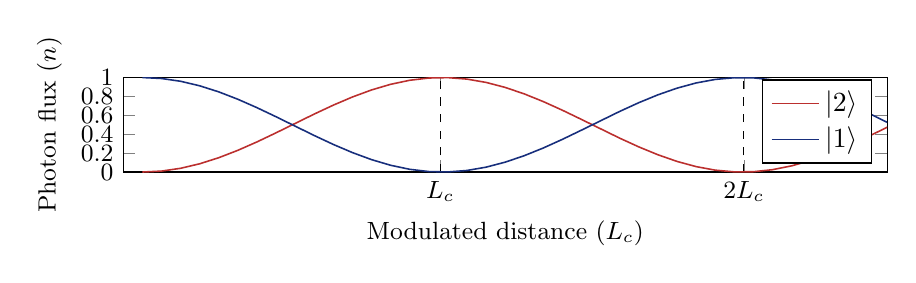
\begin{tikzpicture}

\begin{axis}[%
width=0.8\figW,
height=0.3\figH,
at={(0\figW,0\figH)},
scale only axis,
xmin=0,
xmax=40,
ymin=0,
ymax=1,
xtick={16.6,32.5},
xticklabels={$L_c$, $2L_c$},
ylabel={Photon flux ($n$)},
xlabel={Modulated distance ($L_c$)},
axis background/.style={fill=white}
]
\draw[dashed] (16.6,0) -- (16.6,1);
\draw[dashed] (32.5,0) --(32.5,1);
\addplot [color=mode2, line width = 0.2mm]
table[row sep=crcr]{%
	1	0\\
	2	0.00996671107937885\\
	3	0.039469502998557\\
	4	0.087332192545162\\
	5	0.151646645326416\\
	6	0.229848847065931\\
	7	0.318821122761662\\
	8	0.415016428549883\\
	10	0.613601047346542\\
	11	0.708073418273571\\
	12	0.794250558627674\\
	13	0.868696857770622\\
	14	0.928444376684475\\
	15	0.971111170334332\\
	16	0.994996248300225\\
	17	0.999147387897374\\
	18	0.98339909628973\\
	19	0.948379208167076\\
	20	0.89548385595721\\
	21	0.826821810431809\\
	22	0.745130410670349\\
	23	0.653666434989212\\
	24	0.556076263467524\\
	26	0.358168907268386\\
	27	0.265741664349811\\
	28	0.182653562028683\\
	29	0.112217060744875\\
	30	0.0572402415293425\\
	31	0.0199148566748164\\
	32	0.00172895148838847\\
	33	0.00340754062090554\\
	34	0.0248837040207377\\
	35	0.0653012548250871\\
	36	0.123048872828349\\
	37	0.195824342733872\\
	38	0.280726336212808\\
	39	0.374370078708871\\
	41	0.572750016904308\\
};
\addlegendentry{$\ket{2}$}
\addplot [color=mode1, line width = 0.2mm]
table[row sep=crcr]{%
	1	1\\
	2	0.990033288920621\\
	3	0.960530497001443\\
	4	0.912667807454838\\
	5	0.848353354673584\\
	6	0.770151152934069\\
	7	0.681178877238338\\
	8	0.584983571450124\\
	10	0.386398952653458\\
	11	0.291926581726429\\
	12	0.205749441372326\\
	13	0.131303142229378\\
	14	0.0715556233155255\\
	15	0.028888829665668\\
	16	0.00500375169977474\\
	17	0.000852612102626438\\
	18	0.0166009037102697\\
	19	0.0516207918329243\\
	20	0.10451614404279\\
	21	0.173178189568191\\
	22	0.254869589329651\\
	23	0.346333565010788\\
	24	0.443923736532476\\
	26	0.641831092731614\\
	27	0.734258335650189\\
	28	0.817346437971317\\
	29	0.887782939255125\\
	30	0.942759758470658\\
	31	0.980085143325184\\
	32	0.998271048511612\\
	33	0.996592459379094\\
	34	0.975116295979262\\
	35	0.934698745174913\\
	36	0.876951127171651\\
	37	0.804175657266129\\
	38	0.719273663787192\\
	39	0.625629921291129\\
	41	0.427249983095692\\
};
\addlegendentry{$\ket{1}$}
\end{axis}
\end{tikzpicture}%
	\caption[Modal evolution for multiple coherence lengths]{Modal evolution for multiple coherence lengths. Assuming no losses, the modes will completely transition every integer multiple of the coherence length. Even with an additional phase added to the modulation, the transitions themselves will not physically change, a manifestation of the gauge invariance of the modulation.}
	\label{fig:transition}
\end{figure}


Consider now a direct transition so that the modulation has no spatial dependence ($\delta \cos (\Omega t)$). If the modulation is applied to the entire length of a waveguide, a mode injected in state $\ket{1}$ will harmonically transition to state $\ket{2}$ after passing through one coherence length ($L_c$). If this modulation is extended \textit{beyond} the coherence length, the modes will continue transitioning back and forth, as in Figure \ref{fig:transition}.

However, there is an ambiguity in choosing the time-origin of the modulation. The act of shifting the modulation in time by an amount $t_0$ incorporates an additional phase factor into the modulation,

\begin{equation}
\epsilon'(t) = \delta \cos (\Omega (t-t_0)) = \delta \cos (\Omega t + \phi).
\label{eqn:gaugemod}
\end{equation}

The phase $\phi$ represents a gauge degree of freedom in the modulation, since adjusting the time-origin (a gauge transformation) does not affect the underlying physics in the mode evolution. That is, Figure \ref{fig:transition} will not change regardless of the phase of the modulation and represents a gauge invariance. Both modes will continually transition between each-other in exactly the same shape. In the case of a direct transition with an additional modulation phase, Equation \ref{eqn:cmt} becomes

\begin{equation}
i \dfrac{d}{dx} \begin{bmatrix}
a_1 \\
a_2
\end{bmatrix}
= 
\begin{bmatrix}
0 &  C e^{-(i \phi)} \\
C^\star e^{(i \phi)} & 0 
\end{bmatrix}
\begin{bmatrix}
a_1 \\
a_2
\end{bmatrix}.
\label{cmt:final}
\end{equation}

Thus, an upward transition from $\ket{1} \rightarrow \ket{2}$ will impart a positive phase $\phi$, whereas a downward transition from $\ket{2} \rightarrow \ket{1}$ imparts a $-\phi$ phase. 
This is in direct analogy to a tight-binding model of electrons on a lattice \cite{Paxton2009}. To show this, let $i$ and $j$ represent separate electron sites on a $1D$ lattice, with $b_{i,j}^\dagger$ and $b_{i,j}$ being the creation and annihilation operators of the electrons at their respective sites. Without a magnetic field and assuming no interaction terms, the Hamiltonian is given by

\begin{equation}
H = C_{i,j} b_i^\dagger b_j + C_{j,i} b_j^\dagger b_i,
\label{eqn:hamiltonian}
\end{equation}

where $C_{i,j}$ and $C_{j,i}$ are the `hopping' coefficients between sites $i,j$. In the presence of a magnetic field with corresponding vector potential $\bm{A}$, the Hamiltonian undergoes a gauge transformation \cite{peierls2014} to

\begin{equation}
H' = C_{i,j} \exp({i \frac{e}{\hbar} \int_j^i \bm{A} \cdot d\bm{l}}) b_i^\dagger b_j + C_{j,i} \exp({i \frac{e}{\hbar} \int_i^j \bm{A} \cdot d\bm{l}}) b_j^\dagger b_i.
\end{equation}

In this case, the exponent terms are associated with a constant phase $\phi$ (the AB phase),

\begin{equation}
H' = C_{i,j} e^{i \phi} b_i^\dagger b_j + C_{j,i} e^{-i \phi} b_j^\dagger b_i,
\end{equation}

so that the phase can be linked with the vector potential through

\begin{equation}
\dfrac{e}{\hbar} \int_{i}^{j} \bm{A} \cdot d \bm{l} = \phi.
\end{equation}

Similarly, for the coupled-mode equations \ref{cmt:final}, the corresponding Hamiltonian for the photonic system is given by

\begin{equation}
H = Ce^{-i \phi} a_1^\dagger a_2 + Ce^{i \phi} a_2^\dagger a_1,
\end{equation}

where $a_{1,2}^\dagger$ and $a_{1,2}$ are creation and annihilation operators for the photons in states $\ket{1}$ and $\ket{2}$. This is directly equivalent to the tight-binding Hamiltonian of the electronic system in Equation \ref{eqn:hamiltonian} - the photonic gauge potential can be made explicit by associating

\begin{equation}
\int_{1}^2 \bm{A} \cdot d \bm{l} = \phi,
\label{eqn:gauge}
\end{equation}

where $1$ and $2$ represent the spatial locations of the photonic states $\ket{1}$ and $\ket{2}$ respectively\footnote[1]{Although quantum mechanical in nature, the spatial locations of these photonic states can simply be defined as the centre the photon distribution}. Importantly, since the line integral of equation \ref{eqn:gauge} depends on the direction of propagation, reversing the location of photonic states flips the sign of phase, which shows that a temporal modulation of a permittivity is sufficient to impart a direction dependent phase. \label{sec:gauge} Now, consider the device of Figure \ref{fig:fangab}, consisting of two waveguides coupled together through a dynamic modulation which induces a transition between photonic states $\ket{1}$ and $\ket{2}$. Both upwards and downwards paths are physically passing through the same space, however it is possible to choose different phases for different states along the path. The left hand side is modulated with an additional $\phi(x_1)$ phase, whereas the right hand side is modulated with a $-\phi(x_2)$ phase. For a photon of state $\ket{1}$ injected in the left waveguide coupler, there are two paths it can follow. In the first path, the photon is transitioned to a state $\ket{2}$, propagates along the upper arm in path $P_2$, and transitions back to $\ket{1}$ on the right. In doing so, it acquires a total phase

\begin{equation}
\phi = \int_1^2 \bm{A}(x_1) \cdot d\bm{l} + \phi(P_2) -\int_1^2 \bm{A}(x_1) \cdot d\bm{l}.
\end{equation}

If no modulation is initially applied to the photon, it will remain in state $\ket{1}$ and propagate along the lower path of the interferometer, acquiring only a phase of $\phi(P_1)$. Because of this, the phase difference between both pathways is 

\begin{equation}
\Delta \phi =  \phi(P_2) - \phi(P_1) + \int_1^2 \bm{A}(x_1) \cdot d\bm{l} -\int_1^2 \bm{A}(x_1) \cdot d\bm{l}.
\end{equation}

The line integral is free to be chosen such that it is non-vanishing only at the waveguide couplers, so that
\begin{equation}
 \int_1^2 \bm{A}(x_1) \cdot d\bm{l} -\int_1^2 \bm{A}(x_1) \cdot d\bm{l} = \oint \bm{A} \cdot d\bm{l} = \phi(x_1) - \phi(x_2).
\end{equation}

This phase difference is identical to the phase difference in the AB effect. On the time-reversed path (Fig \ref{sfig:trab}), the phase difference is instead $\phi(x_2) - \phi(x_1)$. The only physically observable quantity is then non-reciprocal.

\begin{figure}[t]
	\centering
	\def\svgwidth{0.5\textwidth}
	\begin{subfigure}{0.5\textwidth}
		\def\svgwidth{0.95\textwidth}
		\centering
		\begin{normalsize}
			\input{figures/photonabtest.pdf_tex}
		\end{normalsize}
		\subcaption{}
	\end{subfigure}%
	\begin{subfigure}{0.5\textwidth}
		\def\svgwidth{0.95\textwidth}
		\centering
		\begin{normalsize}
			\input{figures/photonab2.pdf_tex}
		\end{normalsize}
		\subcaption{}
		\label{sfig:trab}
	\end{subfigure}
	\caption[Aharonov-Bohm effect for photonic transitions]{The Aharonov-Bohm effect for either photonic states $\ket{1}$ and $\ket{2}$ in the \textbf{(a)} forward and \textbf{(b)} time-reversed paths. The structure consists of two waveguides, coupled together through a dynamic modulation (dashed red) that induces a photonic transition between states which imparts an additional phase. Image re-drawn from \cite{Fang2013}.}
	\label{fig:fangab}
\end{figure}
%It is worth pointing out that all operations on the photon modes belong to the group of complex unitary ($U^\dagger = U^{-1}$) $2 \times 2$ matrices with determinant $1$ (known as special unitary $SU(2)$) for both the rotating dielectric and dynamic modulation AB effects. However, the gauge transformation is connected to the arbitrariness in setting a single relative phase factor between the components of states $\ket{1}$ and $\ket{2}$. Since there is only a single such phase factor, the corresponding gauge degree of freedom has only $U(1)$ (group of complex unitary $1 \times 1$ matrices) symmetry.  
    \chapter{Numerical methods in nanophotonics}

\label{chapter:method}
To numerically analyse the non-reciprocity of dynamically modulated structures, a method is required to solve Maxwell's equations for arbitrary permittivity distributions. In almost every case, the electromagnetic problems presented here are difficult, if not impossible to solve analytically. Usually only simple geometries can be considered. Thus, we turn our attention towards numerical solutions instead - namely the finite difference methods, which are a broad class of numerical techniques that solve differential equations by approximating derivatives between finite differences \cite{Champagne2001}.


\begin{figure}[t]
	\centering
	\begin{subfigure}{0.5\textwidth}
		\centering
		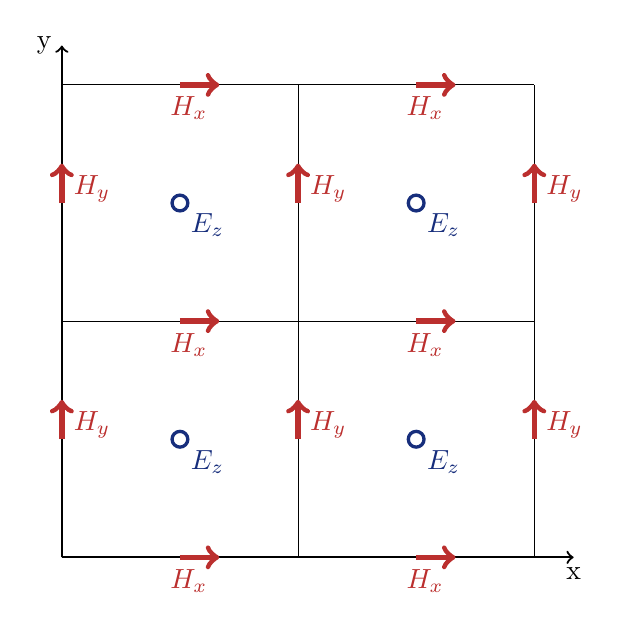
\begin{tikzpicture}
%\node at (-1,6.5) {\textbf{a)}};
\draw[step=3cm,color=black] (0,0) grid (6,6);
\draw[thick,->,color=black] (0,0) -- (6.5,0) node[anchor=north] {x};
\draw[thick,->,color=black] (0,0) -- (0,6.5) node[anchor=east] {y};
%\node at (-0.75,+0.75) {A};
\draw[line width=0.7mm,->,draw=mode2] (1.5,0) -- (2,0) node[anchor=north east] {$\color{mode2} H_x$};
\draw[line width=0.7mm,->,draw=mode2] (4.5,0) -- (5,0) node[anchor=north east] {$\color{mode2} H_x$};
\draw[line width=0.7mm,->,draw=mode2] (1.5,3) -- (2,3) node[anchor=north east] {$\color{mode2} H_x$};
\draw[line width=0.7mm,->,draw=mode2] (4.5,3) -- (5,3) node[anchor=north east] {$\color{mode2} H_x$};
\draw[line width=0.7mm,->,draw=mode2] (1.5,6) -- (2,6) node[anchor=north east] {$\color{mode2} H_x$};
\draw[line width=0.7mm,->,draw=mode2] (4.5,6) -- (5,6) node[anchor=north east] {$\color{mode2} H_x$};

\draw[line width=0.7mm,->,draw=mode2] (0,1.5) -- (0,2) node[anchor=north west] {$\color{mode2} H_y$};
\draw[line width=0.7mm,->,draw=mode2] (3,1.5) -- (3,2) node[anchor=north west] {$\color{mode2} H_y$};
\draw[line width=0.7mm,->,draw=mode2] (6,1.5) -- (6,2) node[anchor=north west] {$\color{mode2} H_y$};
\draw[line width=0.7mm,->,draw=mode2] (0,4.5) -- (0,5) node[anchor=north west] {$\color{mode2} H_y$};
\draw[line width=0.7mm,->,draw=mode2] (3,4.5) -- (3,5) node[anchor=north west] {$\color{mode2} H_y$};
\draw[line width=0.7mm,->,draw=mode2] (6,4.5) -- (6,5) node[anchor=north west] {$\color{mode2} H_y$};

\draw[very thick,->,draw=mode1] (1.5,1.5) circle (0.1cm) node[anchor=north west] {$\color{mode1} E_z$};
\draw[very thick,->,draw=mode1] (4.5,1.5) circle (0.1cm) node[anchor=north west] {$\color{mode1} E_z$};
\draw[very thick,->,draw=mode1] (1.5,4.5) circle (0.1cm) node[anchor=north west] {$\color{mode1} E_z$};
\draw[very thick,->,draw=mode1] (4.5,4.5) circle (0.1cm) node[anchor=north west] {$\color{mode1} E_z$};
\end{tikzpicture}

		\subcaption{}
		\label{sfig:yeegrid}
	\end{subfigure}%
	\begin{subfigure}{0.5\textwidth}
		\centering
		\vspace*{0.25\linewidth}
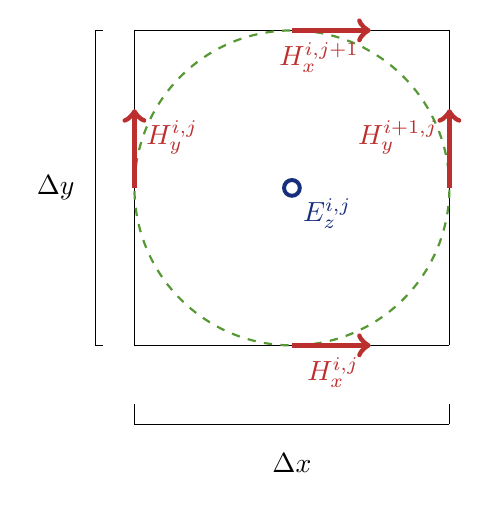
\begin{tikzpicture}
%\node at (-1,5.5) {\textbf{b)}};
\draw[step=4cm,color=black] (0,0) grid (4,4);
\draw[draw=mode3,thick,dashed] (2,2) circle (2cm);
%\draw[thick,->,color=black] (0,0) -- (4.5,0) node[anchor=north] {x};
%\draw[thick,->,color=black] (0,0) -- (0,4.5) node[anchor=east] {y};
\draw[line width=0.7mm,->,draw=mode2] (2,0) -- (3,0) node[anchor=north east] {$\color{mode2} H_x^{i,j}$};
\draw[line width=0.7mm,->,draw=mode2] (2,4) -- (3,4) node[anchor=north east] {$\color{mode2} H_x^{i,j+1}$};
\draw[line width=0.7mm,->,draw=mode2] (0,2) -- (0,3) node[anchor=north west] {$\color{mode2} H_y^{i,j}$};
\draw[line width=0.7mm,->,draw=mode2] (4,2) -- (4,3) node[anchor=north east] {$\color{mode2} H_y^{i+1,j}$};


\draw[line width=0.5mm,->,draw=mode1] (2,2) circle (0.1cm) node[anchor=north west] {$\color{mode1} E_z^{i,j}$};

\draw (0,-1) -- (4,-1);
\draw (0,-1) -- (0,-0.75);
\draw (4,-1) -- (4,-0.75);
\node at (2,-1.5) {$\Delta x$};
\draw (-0.5,0) -- (-0.5,4);
\draw (-0.5,0) -- (-0.4,0);
\draw (-0.5,4) -- (-0.4,4);
\node at (-1,2) {$\Delta y$};
\end{tikzpicture}
		\subcaption{}
		\label{sfig:yeecell}
	\end{subfigure}
	\caption[Electromagnetic field distribution on the Yee grid]{\textbf{a)} Yee grid placement of non-vanishing $E_z$ (blue) and $H_x$, and $H_y$ (red) fields. \textbf{b)} A single cell of the Yee grid, with coordinate placements of the fields. The $H$ field is shown to naturally satisfy the divergence free condition. Likewise, the $E_z$ field sits in the exact centre of the curl.}
	\label{fig:yeegrid}
\end{figure}

The finite difference method replaces all partial derivatives in a differential equation by \textit{approximations}. For a $1D$ function, this can be done by taking the gradient between two points separated by $h$
\begin{equation}
\dfrac{\partial f(x)}{\partial x} = \lim\limits_{h \rightarrow 0} \dfrac{f(a+h) - f(a)}{h} \approx \dfrac{f(a+h)-f(h)}{\Delta h},
\end{equation}
where the accuracy increases as $\Delta h$ approaches 0. For electromagnetic fields however, the $\bm{E}$ and $\bm{H}$ fields are coupled by nature of Maxwell's equations. To discretise these fields in space, the fields are staggered on a $2D$ grid structure known as the Yee grid \cite{Yee1966}, where the electric and magnetic field components are stored at set $i,j$ points on the grid. As shown in Figure \ref{sfig:yeegrid}, the Yee algorithm centres its $\bm{E}$ fields on the faces of a square (in $2D$ TE), and its $\bm{H}$ fields on the edges. This choice ensures that every $\bm{E}$ field component is surrounded by four circulating $\bm{H}$ components \cite{Taflove2005}, naturally satisfying the divergence free conditions.

In deriving these finite differences, the simulation is first assumed to be in $2D$ such that $\partial_z = 0$. Likewise, only the transverse electric (non-vanishing $E_z$, $H_x$, and $H_y$) propagation is considered, and the permeability and permittivity tensors are assumed to be diagonally anisotropic ($\mu_{lm} = \epsilon_{lm} = 0$ if $l \neq m$ ). From this, the curl components of Maxwell's equations, 

\begin{align}
	\nabla \times \bm{E}(\bm{r},t) &= -\mu \dfrac{\partial \bm{H}(\bm{r},t)}{\partial t}, \\
	\nabla \times \bm{H}(\bm{r},t) &= \epsilon \dfrac{\partial \bm{E}(\bm{r},t)}{\partial t},
\end{align}

can be fully vectorised,

\begin{align}
\partial_y E_z &= - \mu_{xx} \partial_t H_x, \\
 \partial_x  E_z &=  \mu_{yy} \partial_t H_y, \\
\partial_x H_y - \partial_y H_x &= \epsilon_{xx}\partial_t E_z.
\end{align}

The partial derivatives are calculated by taking finite differences on the Yee grid, as in Figure \ref{sfig:yeecell}. The notation used here for a single point on the Yee grid is given as $(i,j) = (i \Delta x, j \Delta y)$ where $\Delta$ is the spatial discretisation. Further, any function $f$ evaluated at some discrete point is referred to as $f(i,j) = f^{i,j}$, so that the spatially finite differences take the form 

\begin{align}
\partial_y E_z &= C_x^E|^{i,j} = \dfrac{1}{\Delta y} (E_z^{i,j+1}-E_z^{i,j}), \label{c1}\\
 \partial_x  E_z &= C_y^E|^{i,j} = \dfrac{1}{\Delta x} (E_z^{i+1,j}-E_z^{i,j}), \label{c2} \\
\partial_x H_y - \partial_y H_x &= C_z^H|^{i,j} = \dfrac{1}{\Delta x} (H_y^{i,j}-H_y^{i-1,j}) - \dfrac{1}{\Delta y} (H_x^{i,j}-H_x^{i,j-1}), \label{c3}
\end{align}

where $C$ is used to refer to the curl component of the field at the $i,j$ point on the grid.

\section{Finite difference time domain}

In the finite difference time domain (FDTD) method, \textit{time} is discretised as well as space, and at every time-step all the fields in the simulation are updated based on the previous value of the fields. However, the difficulty in adapting the time domain method to simulate \textit{active} nanophotonic materials is that there is no pre-existing framework for modifying the permittivity tensor while the simulation is running. The effects of motion can be emulated by using a separate source to change the refractive index of the material, but this method introduces its own problems - the pump source can and in most cases will interfere with the original source. The most obvious way to bypass these problems is to directly update the permittivity of the simulation at each time-step. Although this requires having to re-calculate the update coefficients of the simulation every time-step, it is by far the easiest method to implement. Here, a vastly improved convergence time is proposed by moving the equations that are dependent on the permittivity to a single field update equation. In this case, only one update coefficient needs to be calculated per time-step (as opposed to 6) and as will be shown, this coefficient is a relatively inexpensive piecewise matrix division. The only downside of choosing such an update method is that the material permeability tensor becomes entwined in every other coefficient. However, since the permeability coefficients only need to be calculated once, the simulation is not adversely affected.

\subsection{Formulation of the time-domain method}

In the time-domain formulation, $\bm{H}$ fields are calculated at half time steps ($t + \frac{\Delta t}{2}$) and the electric fields at integer steps ($t$), in a central difference scheme, since taking a finite central difference over time would not ensure that the electric fields are located in the mid-point of the magnetic field steps and vice versa. In general, the electric field is much stronger than the magnetic field leading to floating point errors. To rectify this, the electric field is normalised against the impedance,

\begin{equation}
\tilde{\bm{E}} = \sqrt{\dfrac{\epsilon}{\mu}} \bm{E}.
\end{equation}

The partial derivatives are discretised in time as 
\begin{align}
C_x^E\rvert^{i,j}_t &= -\mu_{xx}\rvert^{i,j} (c \Delta t)^{-1} \Big[H_x \rvert_{t+\frac{\Delta t}{2}}^{i,j} - H_x \rvert_{t-\frac{\Delta t}{2}}^{i,j}\Big], \\
C_y^E\rvert^{i,j}_t &= -\mu_{yy} \rvert^{i,j} (c \Delta t)^{-1} \Big[H_x \rvert_{t+\frac{\Delta t}{2}}^{i,j} - H_x \rvert_{t-\frac{\Delta t}{2}}^{i,j}\Big], \\
C_z^H\rvert^{i,j}_{t+\frac{\Delta t}{2}} &= -\epsilon_{zz} \rvert^{i,j} (c \Delta t)^{-1} \Big[E_z \rvert_{t + \Delta t}^{i,j} - E_z \rvert_{t-\Delta t}^{i,j}\Big],
\end{align}

where $C$ refers to the spatial curls of Equations \ref{c1}, \ref{c2}, and \ref{c3}. The above equations can be rearranged to solve for the \textit{future} fields in terms of the past fields,

\begin{align}
H_x \rvert_{t+\frac{\Delta t}{2}}^{i,j} &= H_x \rvert_{t-\frac{\Delta t}{2}}^{i,j} - c \Delta t (\mu_{xx}\rvert^{i,j})^{-1} C_x^E \rvert_t^{i,j}, \\
H_y \rvert_{t+\frac{\Delta t}{2}}^{i,j} &= H_y \rvert_{t-\frac{\Delta t}{2}}^{i,j} - c \Delta t (\mu_{yy}\rvert^{i,j})^{-1} C_y^E \rvert_t^{i,j}, \\
\tilde{E_z} \rvert_{t+\Delta t}^{i,j} &= \tilde{E_z} \rvert_{t-\Delta t}^{i,j} + c \Delta t (\epsilon_{zz} \rvert^{i,j})^{-1} C_z^H \rvert_{t+\frac{\Delta t}{2}}^{i,j}.
\label{eqn:fdtd}
\end{align}

yielding the update equations. Notably, by replacing $\bm{E}$ with $\bm{D} \epsilon^{-1}$, the last field update equation instead becomes

\begin{equation}
\tilde{D_z} \rvert_{t+\Delta t}^{i,j} = \tilde{D_z} \rvert_{t-\Delta t}^{i,j} + c \Delta t  C_z^H \rvert_{t+\frac{\Delta t}{2}}^{i,j},
\end{equation}

where the $E_z$ field can be obtained by,

\begin{equation}
\tilde{E_z} \rvert_{t+\Delta t}^{i,j} =  (\epsilon_{zz} \rvert^{i,j})^{-1} \tilde{D_z} \rvert_{t+\Delta t}^{i,j}.
\end{equation}

These equations are implemented using \textit{MATLAB}, and form the basis of the time-domain simulations (Appendix \ref{app:FDTDeqtn}). However, there are several other components of the simulation that also require taking into account - namely the boundary conditions and source excitations.

\subsection{Boundary conditions \& the Perfectly Matched Layer}
The Perfectly Matched Layer (PML) is an artificial medium that is developed to absorb EM waves incident from any direction with minimal reflection \cite{Berenger1994}. Since EM waves incident on PML do not reflect backwards, a simulation domain surrounded by PML effectively represents an open space, and is used commonly in finite difference methods to simulate spatially unbounded systems (such as waveguides with infinite length, or a point source radiating). Strictly speaking, PML is not a boundary condition, but rather a special type of absorbing material placed adjacent to the boundaries of the simulation. In all simulations presented here, a PML layer of $20 \Delta$ is applied on the boundaries, where $\Delta$ is the chosen spatial discretisation ($\Delta x = \Delta y$). In the case where the discretisation is different along $x$ and $y$, the PML layer extends inward depending on the given discretisation (i.e. the PML width on the left and right sides of the simulation would be $20 \Delta x $, while the width along the top and bottom would be $20 \Delta y $).

\subsection{Modal source}

\begin{figure}[t]
	\centering
	\setlength{\figH}{0.5\textwidth}
	\setlength{\figW}{0.5\textwidth}
	\begin{subfigure}[t]{0.5\textwidth}
		% This file was created by matlab2tikz.
%
%The latest updates can be retrieved from
%  http://www.mathworks.com/matlabcentral/fileexchange/22022-matlab2tikz-matlab2tikz
%where you can also make suggestions and rate matlab2tikz.
%
\definecolor{mycolor1}{rgb}{0.00000,0.44600,0.74200}%
\definecolor{mycolor2}{rgb}{0.46667,0.67451,0.18824}%
%
\begin{tikzpicture}

\begin{axis}[%
width=0.75\figW,
height=0.4\figH,
at={(0\figW,0.6\figH)},
scale only axis,
xlabel={$\text{y (}\mu\text{m)}$},
ylabel={$E_z$ ($V/\mu m$)},
xmin=-1,
xmax=1,
ymin=-1,
ymax=1,
%%
axis background/.style={fill=white}
]
\addplot [color=mycolor1, forget plot]
  table[row sep=crcr]{%
-0.55	0.162969143188896\\
-0.539	0.190666665332457\\
-0.528	0.218213195384856\\
-0.517	0.245586918792565\\
-0.506	0.272766157850501\\
-0.495	0.29972938886896\\
-0.484	0.326455259218582\\
-0.473	0.352922604239856\\
-0.462	0.379110464003759\\
-0.451	0.404998099910273\\
-0.44	0.430565011111631\\
-0.429	0.455790950747268\\
-0.418	0.480655941977656\\
-0.407	0.505140293804285\\
-0.396	0.529224616663298\\
-0.385	0.552889837780404\\
-0.374	0.576117216274925\\
-0.363	0.598888358001009\\
-0.352	0.621185230114262\\
-0.341	0.64299017535225\\
-0.33	0.664285926017585\\
-0.319	0.685055617652497\\
-0.308	0.705282802394075\\
-0.297	0.724951461999608\\
-0.286	0.744046020531692\\
-0.275	0.762551356693074\\
-0.264	0.78045281580146\\
-0.253	0.797736221394798\\
-0.242	0.814387886457854\\
-0.231	0.830394624261188\\
-0.22	0.845743758803939\\
-0.209	0.860423134852165\\
-0.198	0.874421127564773\\
-0.187	0.88772665169942\\
-0.176	0.900329170391103\\
-0.165	0.912218703496477\\
-0.154	0.923385835497295\\
-0.143	0.933821722956714\\
-0.132	0.943518101522557\\
-0.121	0.952467292471992\\
-0.11	0.96066220879244\\
-0.099	0.968096360793897\\
-0.088	0.974763861248226\\
-0.077	0.980659430051355\\
-0.066	0.985778398404671\\
-0.055	0.990116712512328\\
-0.044	0.993670936791508\\
-0.033	0.99643825659312\\
-0.022	0.998416480430764\\
-0.011	0.99960404171621\\
0	1\\
0.011	0.99960404171621\\
0.022	0.998416480430764\\
0.033	0.99643825659312\\
0.044	0.993670936791508\\
0.055	0.990116712512328\\
0.0660000000000001	0.985778398404671\\
0.077	0.980659430051355\\
0.088	0.974763861248226\\
0.099	0.968096360793897\\
0.11	0.96066220879244\\
0.121	0.952467292471992\\
0.132	0.943518101522557\\
0.143	0.933821722956714\\
0.154	0.923385835497295\\
0.165	0.912218703496477\\
0.176	0.900329170391102\\
0.187	0.88772665169942\\
0.198	0.874421127564773\\
0.209	0.860423134852166\\
0.22	0.845743758803939\\
0.231	0.830394624261188\\
0.242	0.814387886457854\\
0.253	0.797736221394798\\
0.264	0.78045281580146\\
0.275	0.762551356693074\\
0.286	0.744046020531692\\
0.297	0.724951461999608\\
0.308	0.705282802394075\\
0.319	0.685055617652497\\
0.33	0.664285926017586\\
0.341	0.64299017535225\\
0.352	0.621185230114262\\
0.363	0.598888358001009\\
0.374	0.576117216274925\\
0.385	0.552889837780404\\
0.396	0.529224616663298\\
0.407	0.505140293804285\\
0.418	0.480655941977656\\
0.429	0.455790950747268\\
0.44	0.430565011111631\\
0.451	0.404998099910273\\
0.462	0.379110464003759\\
0.473	0.352922604239856\\
0.484	0.326455259218582\\
0.495	0.29972938886896\\
0.506	0.272766157850501\\
0.517	0.245586918792565\\
0.528	0.218213195384856\\
0.539	0.190666665332457\\
0.55	0.162969143188896\\
};
\addplot [color=mycolor2, forget plot]
  table[row sep=crcr]{%
0.55	0.162969143188896\\
0.5665	0.126213751586474\\
0.583	0.0977480201332835\\
0.5995	0.0757023329064942\\
0.616	0.0586287394841494\\
0.6325	0.0454058542389436\\
0.649	0.0351652042549129\\
0.6655	0.0272341884326701\\
0.682	0.0210919013639047\\
0.6985	0.0163349205078944\\
0.715	0.0126508095877911\\
0.7315	0.00979759792214484\\
0.748	0.00758788790376361\\
0.7645	0.00587654681255565\\
0.781	0.00455117456638087\\
0.7975	0.00352472133624748\\
0.814	0.00272977015427419\\
0.8305	0.00211410899878382\\
0.847	0.00163730153314944\\
0.8635	0.00126803126612472\\
0.88	0.000982044699351725\\
0.8965	0.000760558368936909\\
0.913	0.000589025156331297\\
0.9295	0.000456178840390737\\
0.946	0.000353294137242572\\
0.9625	0.000273613627723422\\
0.979	0.000211903933250297\\
0.9955	0.000164111989963951\\
1.012	0.000127098845391017\\
1.0285	9.84334935142649e-05\\
1.045	7.62332074348462e-05\\
1.0615	5.90398827504998e-05\\
1.078	4.57242699406538e-05\\
1.0945	3.54118057862857e-05\\
1.111	2.74251724669019e-05\\
1.1275	2.12398116430032e-05\\
1.144	1.64494717097842e-05\\
1.1605	1.27395253818141e-05\\
1.177	9.86630512014263e-06\\
1.1935	7.64109916235286e-06\\
1.21	5.91775702230318e-06\\
1.2265	4.58309039458075e-06\\
1.243	3.54943899956261e-06\\
1.2595	2.74891309726578e-06\\
1.276	2.12893452099064e-06\\
1.2925	1.64878336793324e-06\\
1.309	1.27692353502178e-06\\
1.3255	9.88931442422549e-07\\
1.342	7.65891904244101e-07\\
1.3585	5.9315578797829e-07\\
1.375	4.593778663314e-07\\
1.3915	3.55771668003873e-07\\
1.408	2.75532386366537e-07\\
1.4245	2.13389942945126e-07\\
1.441	1.6526285113195e-07\\
1.4575	1.27990146055217e-07\\
1.474	9.91237738852538e-08\\
1.4905	7.67678048044109e-08\\
1.507	5.94539092237372e-08\\
1.5235	4.60449185826046e-08\\
1.54	3.56601366497229e-08\\
1.5565	2.76174958067431e-08\\
1.573	2.13887591662214e-08\\
1.5895	1.65648262200125e-08\\
1.606	1.28288633093103e-08\\
1.6225	9.93549413818387e-09\\
1.639	7.6946835732708e-09\\
1.6555	5.95925622513484e-09\\
1.672	4.61523003755085e-09\\
1.6885	3.57432999938338e-09\\
1.705	2.76819028315903e-09\\
1.7215	2.14386400950614e-09\\
1.738	1.6603457208912e-09\\
1.7545	1.28587816235452e-09\\
1.771	9.95866479863428e-10\\
1.7875	7.71262841807364e-10\\
1.804	5.97315386330051e-10\\
1.8205	4.62599325945136e-10\\
1.837	3.5826657283971e-10\\
1.8535	2.77464600606733e-10\\
1.87	2.14886373516902e-10\\
1.8865	1.66421782895085e-10\\
1.903	1.28887697105654e-10\\
1.9195	9.98188949560244e-11\\
1.936	7.73061511221986e-11\\
1.9525	5.98708391228043e-11\\
1.969	4.63678158236414e-11\\
1.9855	3.59102089724381e-11\\
2.002	2.78111678442848e-11\\
2.0185	2.1538751207397e-11\\
2.035	1.66809896719056e-11\\
2.0515	1.29188277330889e-11\\
2.068	1.00051683551075e-11\\
2.0845	7.74864375330671e-12\\
2.101	6.00104644766016e-12\\
2.1175	4.64759506482746e-12\\
2.134	3.5993955512593e-12\\
2.1505	2.78760265335345e-12\\
2.167	2.15889819341038e-12\\
2.1835	1.6719891566697e-12\\
2.2	1.29489558542127e-12\\
};
\addplot [color=mycolor2, forget plot]
  table[row sep=crcr]{%
-2.2	1.29489558542127e-12\\
-2.1835	1.67198915666971e-12\\
-2.167	2.15889819341038e-12\\
-2.1505	2.78760265335345e-12\\
-2.134	3.5993955512593e-12\\
-2.1175	4.64759506482746e-12\\
-2.101	6.00104644766016e-12\\
-2.0845	7.74864375330671e-12\\
-2.068	1.00051683551075e-11\\
-2.0515	1.29188277330888e-11\\
-2.035	1.66809896719056e-11\\
-2.0185	2.15387512073972e-11\\
-2.002	2.78111678442848e-11\\
-1.9855	3.59102089724382e-11\\
-1.969	4.63678158236414e-11\\
-1.9525	5.98708391228043e-11\\
-1.936	7.73061511221986e-11\\
-1.9195	9.98188949560244e-11\\
-1.903	1.28887697105654e-10\\
-1.8865	1.66421782895085e-10\\
-1.87	2.14886373516902e-10\\
-1.8535	2.77464600606734e-10\\
-1.837	3.5826657283971e-10\\
-1.8205	4.62599325945136e-10\\
-1.804	5.97315386330049e-10\\
-1.7875	7.71262841807364e-10\\
-1.771	9.95866479863428e-10\\
-1.7545	1.28587816235452e-09\\
-1.738	1.6603457208912e-09\\
-1.7215	2.14386400950613e-09\\
-1.705	2.76819028315904e-09\\
-1.6885	3.57432999938338e-09\\
-1.672	4.61523003755085e-09\\
-1.6555	5.95925622513484e-09\\
-1.639	7.69468357327077e-09\\
-1.6225	9.93549413818387e-09\\
-1.606	1.28288633093103e-08\\
-1.5895	1.65648262200125e-08\\
-1.573	2.13887591662214e-08\\
-1.5565	2.7617495806743e-08\\
-1.54	3.56601366497229e-08\\
-1.5235	4.60449185826046e-08\\
-1.507	5.94539092237372e-08\\
-1.4905	7.67678048044109e-08\\
-1.474	9.91237738852538e-08\\
-1.4575	1.27990146055217e-07\\
-1.441	1.6526285113195e-07\\
-1.4245	2.13389942945126e-07\\
-1.408	2.75532386366537e-07\\
-1.3915	3.55771668003873e-07\\
-1.375	4.59377866331398e-07\\
-1.3585	5.9315578797829e-07\\
-1.342	7.65891904244101e-07\\
-1.3255	9.88931442422549e-07\\
-1.309	1.27692353502178e-06\\
-1.2925	1.64878336793324e-06\\
-1.276	2.12893452099064e-06\\
-1.2595	2.74891309726578e-06\\
-1.243	3.54943899956261e-06\\
-1.2265	4.58309039458075e-06\\
-1.21	5.91775702230318e-06\\
-1.1935	7.64109916235286e-06\\
-1.177	9.86630512014263e-06\\
-1.1605	1.27395253818141e-05\\
-1.144	1.64494717097842e-05\\
-1.1275	2.12398116430033e-05\\
-1.111	2.74251724669019e-05\\
-1.0945	3.54118057862857e-05\\
-1.078	4.57242699406538e-05\\
-1.0615	5.90398827504998e-05\\
-1.045	7.62332074348465e-05\\
-1.0285	9.84334935142649e-05\\
-1.012	0.000127098845391017\\
-0.9955	0.000164111989963951\\
-0.979	0.000211903933250297\\
-0.9625	0.000273613627723422\\
-0.946	0.000353294137242571\\
-0.9295	0.000456178840390737\\
-0.913	0.000589025156331297\\
-0.8965	0.000760558368936911\\
-0.88	0.000982044699351725\\
-0.8635	0.00126803126612472\\
-0.847	0.00163730153314944\\
-0.8305	0.00211410899878382\\
-0.814	0.00272977015427419\\
-0.7975	0.00352472133624748\\
-0.781	0.00455117456638086\\
-0.7645	0.00587654681255565\\
-0.748	0.00758788790376361\\
-0.7315	0.00979759792214484\\
-0.715	0.0126508095877911\\
-0.6985	0.0163349205078944\\
-0.682	0.0210919013639047\\
-0.6655	0.0272341884326702\\
-0.649	0.0351652042549129\\
-0.6325	0.0454058542389434\\
-0.616	0.0586287394841494\\
-0.5995	0.0757023329064942\\
-0.583	0.0977480201332837\\
-0.5665	0.126213751586474\\
-0.55	0.162969143188896\\
};
\addplot [color=black, forget plot]
  table[row sep=crcr]{%
-0.55	-1\\
-0.55	1\\
};
\addplot [color=black, forget plot]
  table[row sep=crcr]{%
0.55	-1\\
0.55	1\\
};
\end{axis}
\node at (-1.5, 3) {\textbf{(b)}};
\node at (-1.5, 7.6) {\textbf{(a)}};

\begin{axis}[%
width=0.75\figW,
height=0.4\figH,
at={(0\figW,0\figH)},
scale only axis,
xlabel={$\text{y (}\mu\text{m)}$},
ylabel={$E_z$ ($V/\mu m$)},
xmin=-1,
xmax=1,
ymin=-1,
ymax=1,
axis background/.style={fill=white}
]
\addplot [color=mycolor1, forget plot]
  table[row sep=crcr]{%
-0.55	-0.325435180556459\\
-0.539	-0.378036364805445\\
-0.528	-0.429443755565253\\
-0.517	-0.479495014462917\\
-0.506	-0.528032085627204\\
-0.495	-0.574901694810093\\
-0.484	-0.619955833408467\\
-0.473	-0.663052225857522\\
-0.462	-0.704054778919932\\
-0.451	-0.74283401145197\\
-0.44	-0.779267463289425\\
-0.429	-0.813240081962109\\
-0.418	-0.844644586015755\\
-0.407	-0.873381803793983\\
-0.396	-0.899360986610489\\
-0.385	-0.922500095322514\\
-0.374	-0.942726059400613\\
-0.363	-0.959975007676623\\
-0.352	-0.974192470041145\\
-0.341	-0.985333549453621\\
-0.33	-0.993363063721798\\
-0.319	-0.998255656602873\\
-0.308	-0.999995877875463\\
-0.297	-0.998578232129555\\
-0.286	-0.994007196120347\\
-0.275	-0.986297204631196\\
-0.264	-0.975472604890298\\
-0.253	-0.961567579685072\\
-0.242	-0.944626039417007\\
-0.231	-0.92470148343789\\
-0.22	-0.901856831105267\\
-0.209	-0.876164223090662\\
-0.198	-0.847704793567987\\
-0.187	-0.816568414001559\\
-0.176	-0.782853409342794\\
-0.165	-0.746666247531806\\
-0.154	-0.708121203284427\\
-0.143	-0.667339997226359\\
-0.132	-0.624451411514044\\
-0.121	-0.57959088315606\\
-0.11	-0.5329000763193\\
-0.099	-0.484526434970522\\
-0.088	-0.434622717265994\\
-0.077	-0.383346513159563\\
-0.066	-0.330859746752479\\
-0.055	-0.277328164956518\\
-0.044	-0.222920814085112\\
-0.033	-0.167809506025369\\
-0.022	-0.112168275676753\\
-0.011	-0.0561728313697414\\
0	0\\
0.011	0.0561728313697414\\
0.022	0.112168275676753\\
0.033	0.167809506025369\\
0.044	0.222920814085112\\
0.055	0.277328164956519\\
0.0660000000000001	0.33085974675248\\
0.077	0.383346513159562\\
0.088	0.434622717265994\\
0.099	0.484526434970522\\
0.11	0.5329000763193\\
0.121	0.57959088315606\\
0.132	0.624451411514044\\
0.143	0.667339997226359\\
0.154	0.708121203284427\\
0.165	0.746666247531806\\
0.176	0.782853409342794\\
0.187	0.816568414001558\\
0.198	0.847704793567987\\
0.209	0.876164223090662\\
0.22	0.901856831105267\\
0.231	0.92470148343789\\
0.242	0.944626039417007\\
0.253	0.961567579685072\\
0.264	0.975472604890298\\
0.275	0.986297204631196\\
0.286	0.994007196120347\\
0.297	0.998578232129555\\
0.308	0.999995877875463\\
0.319	0.998255656602873\\
0.33	0.993363063721798\\
0.341	0.985333549453621\\
0.352	0.974192470041145\\
0.363	0.959975007676623\\
0.374	0.942726059400613\\
0.385	0.922500095322514\\
0.396	0.899360986610489\\
0.407	0.873381803793983\\
0.418	0.844644586015755\\
0.429	0.813240081962109\\
0.44	0.779267463289425\\
0.451	0.74283401145197\\
0.462	0.704054778919932\\
0.473	0.663052225857521\\
0.484	0.619955833408468\\
0.495	0.574901694810093\\
0.506	0.528032085627204\\
0.517	0.479495014462918\\
0.528	0.429443755565253\\
0.539	0.378036364805445\\
0.55	0.325435180556459\\
};
\addplot [color=mycolor2, forget plot]
  table[row sep=crcr]{%
0.55	0.325435180556459\\
0.5665	0.254733633817231\\
0.583	0.199392161863932\\
0.5995	0.156073752872767\\
0.616	0.122166368567749\\
0.6325	0.0956254420382773\\
0.649	0.0748505932706419\\
0.6655	0.0585891285158653\\
0.682	0.0458605046433875\\
0.6985	0.0358972037888675\\
0.715	0.0280984531216947\\
0.7315	0.0219939991002008\\
0.748	0.0172157518538322\\
0.7645	0.013475589888972\\
0.781	0.0105479867738302\\
0.7975	0.00825641221628071\\
0.814	0.00646268753903603\\
0.8305	0.00505865370249478\\
0.847	0.00395964946892375\\
0.8635	0.00309940645057712\\
0.88	0.00242605322043572\\
0.8965	0.00189898753914337\\
0.913	0.00148642809788572\\
0.9295	0.00116349815079926\\
0.946	0.000910725482678128\\
0.9625	0.000712868262170887\\
0.979	0.000557995981089883\\
0.9955	0.000436770061784324\\
1.012	0.000341880754227785\\
1.0285	0.00026760636851771\\
1.045	0.000209468265135284\\
1.0615	0.000163960799370446\\
1.078	0.000128339935946064\\
1.0945	0.000100457787604619\\
1.111	7.86331005701596e-05\\
1.1275	6.15498773436315e-05\\
1.144	4.81780239307226e-05\\
1.1605	3.77112366432596e-05\\
1.177	2.95183831368608e-05\\
1.1935	2.31054460307721e-05\\
1.21	1.80857343644365e-05\\
1.2265	1.41565666841197e-05\\
1.243	1.10810197829738e-05\\
1.2595	8.67364256959257e-06\\
1.276	6.78927363171428e-06\\
1.2925	5.31428821010965e-06\\
1.309	4.1597467876662e-06\\
1.3255	3.25603216336327e-06\\
1.342	2.54865163434724e-06\\
1.3585	1.99495116367379e-06\\
1.375	1.5615434027188e-06\\
1.3915	1.22229448167751e-06\\
1.408	9.56748174490755e-07\\
1.4245	7.48892417590825e-07\\
1.441	5.86193805306755e-07\\
1.4575	4.58841843379115e-07\\
1.474	3.59157390149099e-07\\
1.4905	2.81129615269487e-07\\
1.507	2.20053555208093e-07\\
1.5235	1.72246410657601e-07\\
1.54	1.34825478990197e-07\\
1.5565	1.05534331400792e-07\\
1.573	8.26067534684731e-08\\
1.5895	6.46602449461291e-08\\
1.606	5.06126569674362e-08\\
1.6225	3.9616940013722e-08\\
1.639	3.10100680361566e-08\\
1.6555	2.42730589306995e-08\\
1.672	1.89996806574641e-08\\
1.6885	1.48719560281318e-08\\
1.705	1.16409891350356e-08\\
1.7215	9.11195728293451e-09\\
1.738	7.13236345837111e-09\\
1.7545	5.58284097727075e-09\\
1.771	4.36995584414759e-09\\
1.7875	3.42057281544409e-09\\
1.804	2.67744544865931e-09\\
1.8205	2.09576422351813e-09\\
1.837	1.64045459181173e-09\\
1.8535	1.28406203216824e-09\\
1.87	1.00509658157321e-09\\
1.8865	7.8673702125146e-10\\
1.903	6.15816581167568e-10\\
1.9195	4.82029002572769e-10\\
1.936	3.7730708530252e-10\\
1.9525	2.9533624711304e-10\\
1.969	2.31173763378654e-10\\
1.9855	1.8095072784681e-10\\
2.002	1.41638763109368e-10\\
2.0185	1.10867413764345e-10\\
2.035	8.67812113362179e-11\\
2.0515	6.79277921733508e-11\\
2.068	5.31703219913476e-11\\
2.0845	4.16189463872006e-11\\
2.101	3.2577133888009e-11\\
2.1175	2.54996760966455e-11\\
2.134	1.99598124030538e-11\\
2.1505	1.56234969281634e-11\\
2.167	1.22292560338386e-11\\
2.1835	9.57242183544612e-12\\
2.2	7.49279102033519e-12\\
};
\addplot [color=mycolor2, forget plot]
  table[row sep=crcr]{%
-2.2	-7.49279102033519e-12\\
-2.1835	-9.57242183544618e-12\\
-2.167	-1.22292560338386e-11\\
-2.1505	-1.56234969281634e-11\\
-2.134	-1.99598124030538e-11\\
-2.1175	-2.54996760966454e-11\\
-2.101	-3.2577133888009e-11\\
-2.0845	-4.16189463872006e-11\\
-2.068	-5.31703219913476e-11\\
-2.0515	-6.79277921733503e-11\\
-2.035	-8.67812113362179e-11\\
-2.0185	-1.10867413764346e-10\\
-2.002	-1.41638763109368e-10\\
-1.9855	-1.80950727846811e-10\\
-1.969	-2.31173763378654e-10\\
-1.9525	-2.9533624711304e-10\\
-1.936	-3.7730708530252e-10\\
-1.9195	-4.82029002572769e-10\\
-1.903	-6.1581658116757e-10\\
-1.8865	-7.8673702125146e-10\\
-1.87	-1.00509658157321e-09\\
-1.8535	-1.28406203216824e-09\\
-1.837	-1.64045459181173e-09\\
-1.8205	-2.09576422351813e-09\\
-1.804	-2.6774454486593e-09\\
-1.7875	-3.42057281544409e-09\\
-1.771	-4.36995584414759e-09\\
-1.7545	-5.58284097727075e-09\\
-1.738	-7.13236345837111e-09\\
-1.7215	-9.11195728293448e-09\\
-1.705	-1.16409891350356e-08\\
-1.6885	-1.48719560281318e-08\\
-1.672	-1.89996806574641e-08\\
-1.6555	-2.42730589306995e-08\\
-1.639	-3.10100680361566e-08\\
-1.6225	-3.96169400137222e-08\\
-1.606	-5.06126569674362e-08\\
-1.5895	-6.46602449461291e-08\\
-1.573	-8.26067534684731e-08\\
-1.5565	-1.05534331400791e-07\\
-1.54	-1.34825478990197e-07\\
-1.5235	-1.72246410657601e-07\\
-1.507	-2.20053555208093e-07\\
-1.4905	-2.81129615269487e-07\\
-1.474	-3.59157390149099e-07\\
-1.4575	-4.58841843379116e-07\\
-1.441	-5.86193805306755e-07\\
-1.4245	-7.48892417590825e-07\\
-1.408	-9.56748174490755e-07\\
-1.3915	-1.22229448167751e-06\\
-1.375	-1.5615434027188e-06\\
-1.3585	-1.99495116367379e-06\\
-1.342	-2.54865163434724e-06\\
-1.3255	-3.25603216336327e-06\\
-1.309	-4.1597467876662e-06\\
-1.2925	-5.31428821010965e-06\\
-1.276	-6.78927363171428e-06\\
-1.2595	-8.67364256959257e-06\\
-1.243	-1.10810197829738e-05\\
-1.2265	-1.41565666841197e-05\\
-1.21	-1.80857343644365e-05\\
-1.1935	-2.31054460307721e-05\\
-1.177	-2.95183831368608e-05\\
-1.1605	-3.77112366432596e-05\\
-1.144	-4.81780239307226e-05\\
-1.1275	-6.15498773436317e-05\\
-1.111	-7.86331005701596e-05\\
-1.0945	-0.000100457787604619\\
-1.078	-0.000128339935946064\\
-1.0615	-0.000163960799370446\\
-1.045	-0.000209468265135285\\
-1.0285	-0.00026760636851771\\
-1.012	-0.000341880754227785\\
-0.9955	-0.000436770061784324\\
-0.979	-0.000557995981089883\\
-0.9625	-0.000712868262170886\\
-0.946	-0.000910725482678126\\
-0.9295	-0.00116349815079926\\
-0.913	-0.00148642809788572\\
-0.8965	-0.00189898753914337\\
-0.88	-0.00242605322043572\\
-0.8635	-0.00309940645057712\\
-0.847	-0.00395964946892376\\
-0.8305	-0.00505865370249478\\
-0.814	-0.00646268753903603\\
-0.7975	-0.00825641221628071\\
-0.781	-0.0105479867738302\\
-0.7645	-0.013475589888972\\
-0.748	-0.0172157518538322\\
-0.7315	-0.0219939991002008\\
-0.715	-0.0280984531216947\\
-0.6985	-0.0358972037888675\\
-0.682	-0.0458605046433875\\
-0.6655	-0.0585891285158654\\
-0.649	-0.0748505932706419\\
-0.6325	-0.095625442038277\\
-0.616	-0.122166368567749\\
-0.5995	-0.156073752872766\\
-0.583	-0.199392161863932\\
-0.5665	-0.254733633817231\\
-0.55	-0.325435180556459\\
};
\addplot [color=black, forget plot]
  table[row sep=crcr]{%
-0.55	-1\\
-0.55	1\\
};
\addplot [color=black, forget plot]
  table[row sep=crcr]{%
0.55	-1\\
0.55	1\\
};
\end{axis}
\end{tikzpicture}%
	\end{subfigure}%
	\begin{subfigure}[t]{0.5\textwidth}
		% This file was created by matlab2tikz.
%
%The latest updates can be retrieved from
%  http://www.mathworks.com/matlabcentral/fileexchange/22022-matlab2tikz-matlab2tikz
%where you can also make suggestions and rate matlab2tikz.
%
\begin{tikzpicture}

\begin{axis}[%
width=0.75\figW,
height=0.4\figH,
at={(0\figW,0.6\figH)},
scale only axis,
point meta min=-98.2680517892277,
point meta max=98.2680517892277,
axis on top,
xmin=0,
xmax=5,
xlabel={$\text{x (}\mu\text{m)}$},
ymin=-2.5,
ylabel shift = -10 pt,
ymax=2.5,
ylabel={$\text{y (}\mu\text{m)}$},
axis background/.style={fill=white},
colormap={mymap}{[1pt] rgb(0pt)=(0,0,1); rgb(31pt)=(1,1,1); rgb(32pt)=(1,1,1); rgb(63pt)=(1,0,0)},
%colorbar
]
\addplot [forget plot] graphics [xmin=0, xmax=5, ymin=-2.5, ymax=2.5] {graphs/modes/mode1-1.png};
\draw (0,-0.55) -- (5,-0.55);
\draw (0,0.55) -- (5,0.55);
\draw (0.22,-1) -- (0.22,1);
\end{axis}

\begin{axis}[%
width=0.75\figW,
height=0.4\figH,
at={(0\figW,0\figH)},
scale only axis,
point meta min=-0.00798977562484028,
point meta max=0.00798977562484028,
axis on top,
xmin=0,
xmax=5,
xlabel={$\text{x (}\mu\text{m)}$},
ymin=-2.5,
ymax=2.5,
ylabel shift = -10 pt,
ylabel={$\text{y (}\mu\text{m)}$},
axis background/.style={fill=white},
colormap={mymap}{[1pt] rgb(0pt)=(0,0,1); rgb(31pt)=(1,1,1); rgb(32pt)=(1,1,1); rgb(63pt)=(1,0,0)},
%colorbar
]
\addplot [forget plot] graphics [xmin=0, xmax=5, ymin=-2.5, ymax=2.5] {graphs/modes/mode2-1.png};
\draw (0,-0.55) -- (5,-0.55);
\draw (0,0.55) -- (5,0.55);
\draw (0.22,-1) -- (0.22,1);
\end{axis}
\end{tikzpicture}%
	\end{subfigure}
	\caption[First two transverse electric modes of a slab dielectric waveguide]{The first even and odd modes of a slab dielectric waveguide, \textbf{(a)} $\ket{1}$ (even) and \textbf{(b)} $\ket{2}$ (odd), normalised to unity as returned by the dispersion solver. Blue lines indicate regions inside the waveguide (guided modes), and green lines indicate regions outside the waveguide. On the right, the corresponding shape of the $E_z$ field profile is shown. To excite a total line source, the returned field profile is paired with a sinusoidal oscillation that is written directly into the $E_z$ field at every time-step.}
	\label{fig:modes}
\end{figure}

Since all fields in the simulation are initialised to zero, an excitation of the fields is required. To excite a mode in a wave guide it is insufficient to merely place a point sinusoidal source at some arbitrary location near the guide. Even with a priori knowledge of the mode wavevector $k$ and frequency $\omega$, the source will excite several modes within a range of frequencies. To examine complete mode conversion, an exact known mode is required. If there are multiple modes passing through a modulated region, each will be transitioned up a band of the dispersion relation in turn. The typical method used to excite guided modes in FDTD is to place a \textit{gaussian} source of the form

\begin{equation}
g(t) = e^{-\Big(\dfrac{t-t_0}{\tau}\Big)^2},
\end{equation}

in some off-centre location, where $t_0$ is the pulse centre and $\tau$ is the `spread'. Such a Gaussian source possesses an effectively infinite range of frequencies. After propagating through the waveguide, modes within range of the spread frequency are excited.

Instead of attempting to generate modes via Gaussian sources, a waveguide dispersion relation solver is implemented in \textit{MATLAB} to both calculate dispersion relations, and return electric field amplitudes in the exact shape of the required mode (Appendix \ref{app:FDTD}), by numerically solving the transcendental equation \cite{Rana2017}

\begin{equation}
\begin{bmatrix}
\tan(k_x d) \\
- \cot(k_x d )
\end{bmatrix}
=
\Big[\dfrac{\omega^2 \mu_0 (\epsilon_1 - \epsilon_2)}{k_z^2}-1\Big]^{\frac{1}{2}},
\end{equation}

where $k_x$ and $k_z$ are wavevector components in $x$ and $z$ respectively, $\omega$ is the given frequency, $\epsilon_1$ is the waveguide permittivity, $\epsilon_2$ is the surrounding permittivity, and $d$ is the width of the waveguide.

To verify the implementation wherever dispersion relations are calculated, a comparison is also made to the open source \textit{MPB} photonic bandstructure program \cite{Johnson2001}, which instead makes use frequency iterative methods. Having a numerical solver for the bands means that a source can be excited directly by choosing an input region, passing the parameters of the wave guide to the dispersion solver, and obtaining a mode at a pre-defined frequency (or equivalently, wavevector). This mode shape is then paired with a sinusoidally oscillating source at the given frequency. This is demonstrated in Figure \ref{fig:modes}, where the output of the mode solver is shown for the first even $\ket{1}$ and odd $\ket{2}$ TE modes for a waveguide of width $1.1 \mu m$ and relative permittivity $10$. 


\subsection{Demonstration of direct photonic transitions}
\label{sec:demonstration}
%\begin{figure}[t]
%	\centering
%	\setlength{\figH}{1\textwidth}
%	\setlength{\figW}{1\textwidth}
%	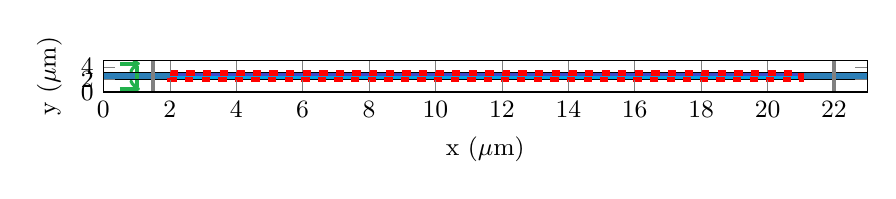
\begin{tikzpicture}
    \begin{axis}[%
width=0.8\figW,
height=0.1\figH,
at={(0\figW,0\figH)},
scale only axis,
axis on top,
xmin=0,
xmax=23,
xlabel={$\text{x (}\mu\text{m)}$},
ymin=0,
ymax=5,
ylabel={$\text{y (}\mu\text{m)}$},
axis background/.style={fill=white},
]
\fill[fill=eps] (0,1.95) rectangle (23,3.05);
\fill[fill=epsilon] (2,2.5) rectangle (21,3.05);
\fill[fill=modup] (2,2.5) rectangle (21,1.95);
\draw[draw=src, line width=0.5mm] (1,0.8) -- (1,4.2);
\draw[line width=0.5mm, draw=src, ->] (0.5,4.5) -- (1.1,4.5);
\draw[line width=0.5mm, draw=src, ->] (0.5,0.5) -- (1.1,0.5);
%\draw[pattern=north west lines, pattern color=black] (0,0) rectangle (60,0.5);
%\draw[pattern=north west lines, pattern color=black] (0,0) rectangle (0.5,5);
%\draw[pattern=north west lines, pattern color=black] (0,5) rectangle (60,4.5);
%\draw[pattern=north west lines, pattern color=black] (60,0) rectangle (59.5,4.5);
\draw (0,1.95) -- (24.2,1.95) -- (24.2,1.5) -- (35.8,1.5) -- (35.8,1.95) -- (60,1.95);
\draw (0,3.05) -- (24.2,3.05) -- (24.2,3.5) -- (35.8,3.5) -- (35.8,3.05) -- (60,3.05);
\draw[draw=red, dashed, line width=0.7mm] (2,3.05) -- (21,3.05) -- (21,1.95) -- (2,1.95) -- (2,3.05);
\draw[draw=gray, line width = 0.5mm] (1.5,0) -- (1.5,5);
\draw[draw=gray, line width = 0.5mm] (22,0) -- (22,5);
\end{axis}
\end{tikzpicture}
%	\caption[The weakly modulated waveguide structure]{The modulated waveguide structure. The dark blue region is a material of unity permeability and permittivity of $\epsilon_{wg} = 12.25$. The light blue sections are regions where the permittivity is modulated by an amount $0.1 \epsilon_{wg} \cos(\omega t + \phi)$, with $\phi=0$ on the left and $\phi=\frac{\pi}{2}$ on the right. The modulation region is chosen to only cover the upper half of the waveguide to maximise the coupling.}
%	\label{fig:cavity}
%\end{figure} 

\begin{figure}[t]
	\centering
	\setlength{\figH}{\textwidth}
	\setlength{\figW}{\textwidth}
	% This file was created by matlab2tikz.
%
%The latest updates can be retrieved from
%  http://www.mathworks.com/matlabcentral/fileexchange/22022-matlab2tikz-matlab2tikz
%where you can also make suggestions and rate matlab2tikz.
%
\definecolor{mycolor1}{rgb}{0.00000,0.44700,0.74100}%
\definecolor{mycolor2}{rgb}{0.85000,0.32500,0.09800}%
\definecolor{mycolor3}{rgb}{0.92900,0.69400,0.12500}%
\definecolor{mycolor4}{rgb}{0.49400,0.18400,0.55600}%
%
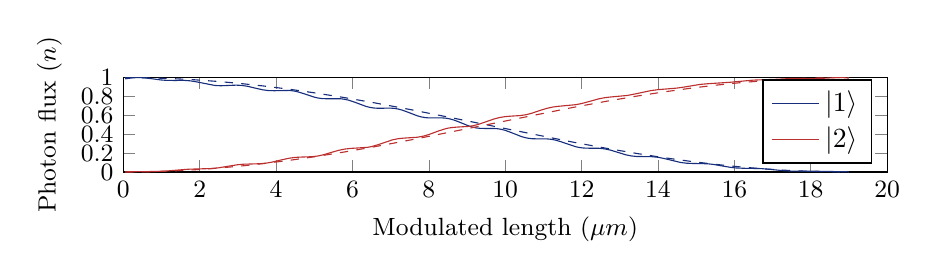
\begin{tikzpicture}

\begin{axis}[%
width=0.8\figW,
height=0.3\figH,
at={(0\figW,0\figH)},
scale only axis,
xmin=0,
xmax=20,
ymin=0,
ymax=1,
xlabel = {Modulated length ($\mu m$)},
ylabel = {Photon flux ($n$)},
axis background/.style={fill=white}
]
\addplot [color=mode1]
  table[row sep=crcr]{%
0.0500000000000007	0.986694052000001\\
0.25	0.997355889000001\\
0.399999999999999	1\\
0.550000000000001	0.997254714\\
0.75	0.987333306\\
1	0.973848500999999\\
1.15	0.969599106\\
1.35	0.969195889000002\\
1.6	0.969643087000001\\
1.75	0.965274509\\
1.9	0.955816716000001\\
2.4	0.916140681000002\\
2.55	0.913152491000002\\
2.75	0.916187747999999\\
2.95	0.919540203\\
3.1	0.916830467\\
3.25	0.907757176000001\\
3.45	0.888638635\\
3.65	0.870176603000001\\
3.8	0.862215405000001\\
3.95	0.860582315999999\\
4.35	0.863610502\\
4.45	0.859005038999999\\
4.55	0.850809978000001\\
4.7	0.832837961999999\\
5	0.792670651000002\\
5.1	0.783428644000001\\
5.2	0.777721363000001\\
5.35	0.775212203999999\\
5.7	0.775125292999999\\
5.8	0.769786952\\
5.9	0.760574705\\
6.05	0.740514132000001\\
6.35	0.695389793\\
6.45	0.684781181000002\\
6.55	0.678039108\\
6.65	0.675047397\\
6.8	0.675445301\\
7	0.676491379000002\\
7.1	0.67344808\\
7.2	0.666571595000001\\
7.3	0.655718989\\
7.45	0.633696021999999\\
7.7	0.594953963000002\\
7.8	0.583650304999999\\
7.9	0.576265646\\
8	0.572737298\\
8.15	0.572549955\\
8.35	0.573068835000001\\
8.45	0.56976654\\
8.55	0.562569932999999\\
8.65	0.551291265\\
8.8	0.528351226000002\\
9.05	0.487278348\\
9.15	0.474875100999999\\
9.25	0.46642327\\
9.35	0.461965199000002\\
9.5	0.460841005999999\\
9.7	0.46120307\\
9.8	0.458263487\\
9.9	0.451640051999998\\
10	0.441052800000001\\
10.15	0.419146350999998\\
10.4	0.378993314999999\\
10.5	0.366502645000001\\
10.6	0.357714438999999\\
10.7	0.352761213000001\\
10.85	0.350919177000002\\
11.1	0.350448699000001\\
11.2	0.346637943000001\\
11.3	0.339333867000001\\
11.45	0.322084674999999\\
11.85	0.267281336\\
11.95	0.259008083000001\\
12.05	0.254180084000001\\
12.2	0.252071075\\
12.45	0.251483852\\
12.6	0.245501526999998\\
12.75	0.232642741999999\\
12.9	0.214400477000002\\
13.15	0.183089106000001\\
13.3	0.170449332\\
13.45	0.164485076999998\\
13.65	0.163598780000001\\
13.85	0.162269086999999\\
14	0.15603861\\
14.15	0.144254965999998\\
14.6	0.100622414\\
14.75	0.0933171520000009\\
14.9	0.0907820719999997\\
15.3	0.0875060310000002\\
15.45	0.0807486439999998\\
15.7	0.0631197109999988\\
15.9	0.049559704\\
16.05	0.0429908810000015\\
16.25	0.0396613419999987\\
16.7	0.0365461459999992\\
16.95	0.0276234510000002\\
17.3	0.0134594620000001\\
17.5	0.0096070250000011\\
17.8	0.0091715189999988\\
18.2	0.00795627600000159\\
19	0.00205285599999883\\
};
\addlegendentry{$\ket{1}$}
\addplot [color=mode2]
  table[row sep=crcr]{%
0.0500000000000007	0.00221802900000156\\
0.850000000000001	0.00582627400000035\\
1.1	0.0097343770000009\\
1.4	0.0198939749999987\\
1.7	0.029623492999999\\
1.95	0.0329643090000005\\
2.3	0.03675286\\
2.5	0.044828128999999\\
2.75	0.0616579629999983\\
3	0.0775024649999985\\
3.15	0.0828504069999987\\
3.4	0.0857207429999995\\
3.6	0.0886016000000005\\
3.75	0.0947910790000002\\
3.9	0.10543096\\
4.15	0.129462504999999\\
4.35	0.146831486\\
4.5	0.154842831\\
4.65	0.158284257999998\\
4.95	0.162379112\\
5.1	0.170050675999999\\
5.25	0.183598153999998\\
5.5	0.213877024999999\\
5.65	0.230807343999999\\
5.8	0.243064097000001\\
5.95	0.249822298000002\\
6.4	0.261662499\\
6.5	0.269430125\\
6.65	0.286602654999999\\
7.05	0.340965801999999\\
7.2	0.353101950999999\\
7.35	0.359084478\\
7.7	0.368252758000001\\
7.85	0.379247058000001\\
8	0.396694839999999\\
8.25	0.433824799\\
8.4	0.453948307000001\\
8.5	0.463998901\\
8.6	0.470805353999999\\
8.75	0.475859165999999\\
9.05	0.482985608\\
9.15	0.489356490999999\\
9.3	0.504590070999999\\
9.5	0.532427214999998\\
9.7	0.560563994999999\\
9.85	0.576667987\\
10	0.586645054000002\\
10.15	0.591531657000001\\
10.4	0.597876745000001\\
10.55	0.607136604000001\\
10.7	0.622735303999999\\
10.95	0.656699764999999\\
11.1	0.675062894\\
11.25	0.688151403999999\\
11.4	0.695901053\\
11.85	0.712871225000001\\
12	0.724777358000001\\
12.2	0.746461385\\
12.45	0.774416689999999\\
12.6	0.786430815999999\\
12.75	0.793687932000001\\
13.2	0.810600870999998\\
13.4	0.826260157\\
13.8	0.860627362999999\\
14	0.871852792999999\\
14.25	0.880085314999999\\
14.5	0.888553403\\
14.7	0.900148941000001\\
15.1	0.927127182\\
15.3	0.934342208\\
15.9	0.950310096999999\\
16.5	0.972822297\\
16.75	0.976590496\\
17.1	0.981624049000001\\
17.55	0.991271328\\
17.8	0.98955943\\
18.05	0.988140959999999\\
18.3	0.991819562\\
18.7	0.999900176000001\\
18.85	0.999009899000001\\
19	0.99430156\\
};
\addlegendentry{$\ket{2}$}
\addplot [color=mode1, dashed, forget plot]
  table[row sep=crcr]{%
0.0500000000000007	0.999982913\\
0.649999999999999	0.997115031\\
1.25	0.989358422999999\\
1.85	0.976789367999999\\
2.45	0.959531474999999\\
3.05	0.937754459000001\\
3.7	0.909312407000002\\
4.35	0.876146941000002\\
5.05	0.835588004000002\\
5.8	0.787164331\\
6.6	0.730670581000002\\
7.5	0.662349734999999\\
8.65	0.570041348\\
11.75	0.318246015\\
12.65	0.251194237\\
13.45	0.196166152\\
14.15	0.152340571\\
14.85	0.113167183000002\\
15.5	0.0814167609999998\\
16.15	0.054496738000001\\
16.75	0.0342044560000012\\
17.35	0.0184928980000016\\
17.95	0.00751657500000036\\
18.55	0.00138343000000063\\
19	0\\
};
\addplot [color=mode2, dashed, forget plot]
  table[row sep=crcr]{%
0.0500000000000007	1.70871999998212e-05\\
0.649999999999999	0.00288496900000013\\
1.25	0.0106415770000012\\
1.85	0.0232106320000014\\
2.45	0.0404685250000014\\
3.05	0.0622455409999993\\
3.7	0.0906875929999984\\
4.35	0.123853059000002\\
5.05	0.164411995999998\\
5.8	0.212835669\\
6.6	0.269329419000002\\
7.5	0.337650265000001\\
8.65	0.429958652\\
11.75	0.681753985\\
12.65	0.748805763\\
13.45	0.803833848\\
14.15	0.847659429\\
14.85	0.886832816999998\\
15.5	0.918583239\\
16.15	0.945503261999999\\
16.75	0.965795543999999\\
17.35	0.981507101999998\\
17.95	0.992483425\\
18.55	0.998616569999999\\
19	1\\
};
\end{axis}
\end{tikzpicture}%
	\caption[Power spectrum of mode transitions]{Normalised amplitude of the modes along the modulated region. Simulation results are in solid lines. Theoretical results from equation \ref{eqn:theorymode} are shown in dashed lines. Mode $\ket{1}$ vanishes at $19 \mskip3mu \mu m$, giving the value of the coherence length. As the amplitude of the first mode decreases, the second mode increases in turn. The discrepancy between theoretical and simulation is largely due to the generation of spurious side band frequency components, which theoretical treatments can not accurately predict.}
	\label{fig:coherencelengthtd}
\end{figure} 

Here, a direct mode conversion is demonstrated through FDTD as a method of verifying the \textit{MATLAB} implementation of the update equations (\ref{eqn:fdtd}). The waveguide is chosen to be of length $23\mskip3mu \mu m$ and width $1.1\mskip3mu \mu m$. From a dispersion relation calculation, such a waveguide supports the TE modes $\ket{1}$ at frequency $\omega_1 = 0.129 \mskip3mu (2 \pi c/a)$, and $\ket{2}$ at $\omega_2 = 0.199 \mskip3mu (2 \pi c/a)$, at the same wavevector $k$. A modulation of $\delta \cos (\Omega t + \phi)$ is initially applied from $2  \mskip3mu \mu m$ to $21 \mskip3mu \mu m$. This modulation here is a direct transition, as $\Delta k = 0$ \footnote{Such a choice of spatially independent modulation leads to a strictly \textit{reciprocal} mode conversion. On the reverse path (RL), phase matching is still satisfied (no wavevector shift is applied) allowing the back-propagating mode to transition regardless.}. A modal line source is excited at $x = 1 \mskip3mu \mu m$ that extends from $y=1$ to $y=3 \mskip3mu \mu m$, with the spatial discretisation chosen as $\Delta x = \Delta y = 0.04 \mskip3mu \mu m$. To obtain the coherence length, the amplitudes of both modes are sampled throughout the modulated region continuously, by calculating a Fourier transform over the length simulation.

 A detector ($D_2$) is placed at $22 \mskip3mu \mu m$ to collect the incident field after modulation, and another detector ($D_1$) placed in the region between the source and the beginning of modulation ($1.5 \mskip3mu \mu m$). To ensure the steady state solution is reached, the simulation is run for $10 000$ time steps (corresponding to a time of around $850 \mskip3mu fs$). To obtain the coherence length, the modulation region is first extended to $25 \mu m$, and the amplitudes of modes $\ket{1}$ and $\ket{2}$ are sampled with a Fourier transform along the entire length of the waveguide, as shown in figure \ref{fig:coherencelengthtd}. The coherence length is then numerically determined to be $19 \mu m$, based on how the first mode vanishes at that point. Note the discrepancy between theoretical and simulation, this is largely because the theoretical treatment of photonic transitions is restricted to only coupling between two adjacent modes. In reality, the modulation can generate backward propagating modes (such that $k \rightarrow -k$), as well as modes at higher sidebands, and thus power is lost to these spurious modes - which the semi-analytic coupled mode theory can not predict. With only a temporal modulation, scattering in the guide can transition backward reflected waves into higher order modes. This only occurs because reciprocity is not broken in the waveguide so that light is free to pass in both directions. Coupled mode theory does not predict such oscillations, as it is derived to assume the coupling is only between two exact modes.

Importantly, perfect mode conversion is observed in Figure \ref{fig:reciprocalmode} agreeing with the expected theory. The Fourier transform of the detector outputs illustrates the input $\ket{1}$ mode at $\omega_1 = 0.129 \mskip3mu (2\pi c/a)$ and output in mode $\ket{2}$ at $\omega_2 = 0.199 \mskip3mu (2\pi c/a)$. Additionally, a weak higher order mode $\ket{3}$ is observed at frequency $\omega_3 = 0.269 \mskip3mu (2\pi c/a)$ in the output. The existence of the higher order mode is attributed to a further direct transition of the 2nd mode. 

\begin{figure}[t]
	\centering
	\setlength{\figH}{\textwidth}
	\setlength{\figW}{\textwidth}
	\begin{subfigure}[t]{\textwidth}
		\centering
		% This file was created by matlab2tikz.
%
%The latest updates can be retrieved from
%  http://www.mathworks.com/matlabcentral/fileexchange/22022-matlab2tikz-matlab2tikz
%where you can also make suggestions and rate matlab2tikz.
%
\begin{tikzpicture}

\begin{axis}[%
width=0.75\figW,
height=0.06\figH,
at={(0\figW,0\figH)},
scale only axis,
point meta min=-4.99371933183411,
point meta max=4.99371933183411,
axis on top,
xmin=0,
xmax=23,
xlabel={$\text{x (}\mu\text{m)}$},
ymin=-2.5,
ymax=2.5,
ylabel={$\text{y (}\mu\text{m)}$},
axis background/.style={fill=white},
colormap={mymap}{[1pt] rgb(0pt)=(0,0,1); rgb(31pt)=(1,1,1); rgb(32pt)=(1,1,1); rgb(63pt)=(1,0,0)},
colorbar,
colorbar style={width=.01\linewidth, at={(1.02,0.03\figH)}, anchor=east,ytick={-4,4},title={$E_z$ ($V/\mu m$)}}
]
\addplot [forget plot] graphics [xmin=0, xmax=23, ymin=-2.5, ymax=2.5] {graphs/fdtd/reciprocal/fieldconvertFINAL-1.png};
\draw (0,0.55) -- (23,0.55);
\draw (0,-0.55) -- (23,-0.55);
\end{axis}
\end{tikzpicture}%
	\end{subfigure}
	\begin{subfigure}[t]{\textwidth}
		\centering
	% This file was created by matlab2tikz.
%
%The latest updates can be retrieved from
%  http://www.mathworks.com/matlabcentral/fileexchange/22022-matlab2tikz-matlab2tikz
%where you can also make suggestions and rate matlab2tikz.
%
\definecolor{mycolor1}{rgb}{0.00000,0.44700,0.74100}%
\definecolor{mycolor2}{rgb}{0.85000,0.32500,0.09800}%
%
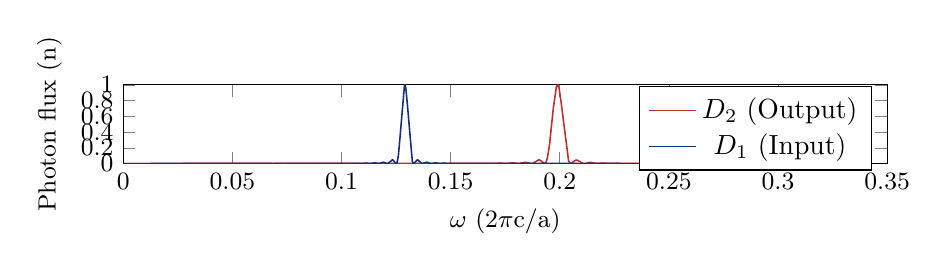
\begin{tikzpicture}

\begin{axis}[%
width=0.8\figW,
height=0.25\figH,
at={(0\figW,0\figH)},
scale only axis,
xmin=0,
yticklabel style={/pgf/number format/fixed},
xticklabel style={/pgf/number format/fixed},
xmax=0.35,
xlabel={$\omega\text{ (2}\pi\text{c/a)}$},
ymin=0,
ymax=1,
ylabel={Photon flux (n)},
axis background/.style={fill=white}
]
\addplot [color=mode2, line width = 0.2mm]
  table[row sep=crcr]{%
0	6.90869460877597e-05\\
0.117304596739771	0.000462718159760289\\
0.125978998091404	0.000297382378737554\\
0.128180961511434	0.000352644284727033\\
0.132184531366034	0.00136759188320346\\
0.135987922727904	0.000623862971118383\\
0.139057326283097	0.000828198409184244\\
0.141859825181316	0.000660951377172703\\
0.144595597915293	0.000880803909467209\\
0.147264644485026	0.000661010805538709\\
0.149933691054759	0.00104813172839613\\
0.152602737624492	0.000634754192933906\\
0.155471962686955	0.00129608157213545\\
0.158074283092445	0.000596691713695474\\
0.161210412811882	0.00169181178897571\\
0.163679280888885	0.000537857283981813\\
0.165080530337995	0.00187689072933561\\
0.166348327458618	0.00275244484186965\\
0.167349219922268	0.00209827972595544\\
0.169217552521081	0.000402898721760359\\
0.170151718820488	0.00130727836939815\\
0.172286956076274	0.00435614718142729\\
0.173154396211437	0.0034196358130536\\
0.175089454974494	0.00033783528024256\\
0.175823442781171	0.00131201058789543\\
0.178292310858174	0.00759803878669318\\
0.179026298664851	0.0062312771917945\\
0.18102808359215	0.00027904961622327\\
0.18162861907034	0.00151927091309956\\
0.182562785369747	0.0071249763018022\\
0.184097487147343	0.0157152582445836\\
0.18463129646129	0.0151205659351976\\
0.185365284267967	0.0106805311974563\\
0.186966712209806	0.000217090110192109\\
0.18743379535951	0.00173028610106374\\
0.1880343308377	0.0084738673201854\\
0.19043647275046	0.0469296521087703\\
0.19083682973592	0.0445060834473012\\
0.191504091378353	0.0318423586778283\\
0.192972066991706	0.000166588713402138\\
0.193238971648679	0.00213547272719938\\
0.193639328634139	0.0146414049227928\\
0.194306590276573	0.0681609150338081\\
0.195240756575979	0.223097752723171\\
0.197042363010549	0.699960097651519\\
0.198443612459659	0.97368804999049\\
0.198977421773606	1\\
0.199244326430579	0.993817527270956\\
0.199711409580282	0.952638619245898\\
0.200578849715445	0.788690155144477\\
0.204048610256099	0.0333279927147885\\
0.204849324227019	0.000948272372751857\\
0.205049502719749	0.000118381422221425\\
0.205383133540965	0.00313178746896159\\
0.206250573676128	0.0239506141498314\\
0.207384918468265	0.0440519518109421\\
0.207585096960995	0.0445989555779434\\
0.207985453946455	0.0428311430828778\\
0.208652715588888	0.0331925278406733\\
0.210721226680431	0.00079239642971829\\
0.211054857501648	9.47016444752258e-05\\
0.211588666815595	0.00170767127777194\\
0.213790630235625	0.0144060916740212\\
0.214391165713814	0.0130535901147792\\
0.215525510505951	0.00602516654503416\\
0.216726581462331	0.000416984425901878\\
0.217260390776278	0.000189870516005719\\
0.217994378582954	0.0018535808012381\\
0.219729258853281	0.00651767931620006\\
0.220463246659957	0.00597110525495781\\
0.221797769944824	0.00218566643168572\\
0.222932114736961	0.000164174141741524\\
0.223732828707881	0.00057208555282684\\
0.226068244456397	0.00343010723270276\\
0.227069136920047	0.00243806872616137\\
0.22893746951886	0.000187253079213079\\
0.230005088146753	0.000596664568742744\\
0.232006873074053	0.00195118002163341\\
0.233274670194676	0.00126137393949266\\
0.235076276629246	0.00020982260593283\\
0.236610978406843	0.000746757395190256\\
0.238279132512926	0.00113072027948724\\
0.242416154696012	0.000484357236604227\\
0.244618118116042	0.000657299140288004\\
0.248087878656696	0.000384430844256878\\
0.251424186868862	0.000368964292266183\\
0.258296981785925	0.000433298881798105\\
0.261166206848388	0.000634423609358281\\
0.263501622596904	0.000373648648806624\\
0.264569241224798	0.0015449099263416\\
0.265837038345421	0.00477866594844389\\
0.268639537243641	0.0126852117739487\\
0.269440251214561	0.0126759087932213\\
0.270374417513967	0.0109087311214555\\
0.274511439697054	0.000264945650912729\\
0.275779236817677	0.000339848587029845\\
0.277914474073463	0.000734609053077762\\
0.282118222420793	0.000296144777373719\\
0.28465381666204	0.000269904006837685\\
0.287523041724503	0.000192366491871265\\
0.290525719115452	0.000207772302890374\\
0.293461670342159	0.000173096362881653\\
0.296464347733109	0.000200634199863048\\
0.299533751288302	0.000165982888722382\\
0.302669881007738	0.000170916018330081\\
0.305872736891418	0.000176753006553287\\
0.309275771267828	9.51751238431608e-05\\
0.31594838769216	4.70114322019821e-05\\
0.333564095052399	5.21973813545351e-05\\
};
\addlegendentry{$D_2$ (Output)}

\addplot [color=mode1, line width = 0.2mm]
  table[row sep=crcr]{%
0	9.84499576692777e-05\\
0.0667261642433286	0.000428427228356787\\
0.068661223006385	6.13305372691997e-05\\
0.0702626509482249	0.000374831456357638\\
0.0717306265615782	0.000351368916442052\\
0.0734655068319048	0.000123256754796186\\
0.0755340179234478	0.000487187979007375\\
0.0774690766865045	0.000131415964435666\\
0.0794708616138042	0.000583041003948681\\
0.0814059203768609	0.000123277227918717\\
0.0834744314684039	0.000702983462822937\\
0.0853427640672171	0.000109068278802305\\
0.0874780013230037	0.000831396473917945\\
0.0893463339218168	0.000121856262543352\\
0.0914148450133601	0.00105879897365746\\
0.0933499037764167	0.000146538997274126\\
0.0954184148679598	0.00133377399004853\\
0.0973534736310164	0.000164486871907288\\
0.0994219847225595	0.00167874640134524\\
0.101290317321373	0.000160923180471562\\
0.102558114441996	0.00216389097464975\\
0.103292102248673	0.00241524257214309\\
0.105227161011729	0.000129803064990774\\
0.106094601146892	0.00184495690976028\\
0.107095493610542	0.00341718315492523\\
0.107829481417219	0.00230563928595595\\
0.109030552373599	3.30608605381144e-05\\
0.109697814016032	0.00127003609093057\\
0.111099063465142	0.00515347101819752\\
0.111699598943332	0.00401678469918942\\
0.113034122228199	4.04586502038562e-05\\
0.113567931542145	0.00134799796618279\\
0.115102633319742	0.00850395286559102\\
0.115569716469445	0.00743269865808505\\
0.117037692082798	3.74847521795729e-05\\
0.117438049068258	0.00142940397848035\\
0.118172036874935	0.00887593076299287\\
0.119172929338585	0.0165955252138328\\
0.119573286324045	0.0148584893668855\\
0.120507452623451	0.00318449807704857\\
0.120974535773155	3.8371287889083e-05\\
0.121308166594371	0.00168441406063069\\
0.121841975908318	0.0122478495686607\\
0.123309951521671	0.0479045978139261\\
0.123643582342888	0.0439487047529896\\
0.124310843985321	0.0199913970337922\\
0.124978105627754	7.54562746287935e-05\\
0.125178284120484	0.0021059847279834\\
0.125511914941701	0.0202086890353097\\
0.126045724255648	0.0992294441321038\\
0.126913164390811	0.370292542497138\\
0.128848223153867	0.995328829661499\\
0.128981675482354	1\\
0.129115127810841	0.997360946624525\\
0.129448758632057	0.959402049129023\\
0.130116020274491	0.769030373043881\\
0.132451436023007	0.0240565336073533\\
0.132985245336954	4.48384782758549e-05\\
0.133252149993927	0.00335261462704084\\
0.13472012560728	0.0467472013009338\\
0.134987030264254	0.0448349887504631\\
0.135587565742444	0.0297499812744499\\
0.136855362863067	0.000366988704898708\\
0.13732244601277	0.00146520772117942\\
0.138857147790367	0.0163715424299369\\
0.139257504775827	0.0147236468621543\\
0.140992385046153	2.33173488148886e-05\\
0.141459468195857	0.00125620832661566\\
0.14292744380921	0.00815906522325061\\
0.143461253123156	0.00666437845181656\\
0.145062681064996	3.97393674484992e-05\\
0.145663216543186	0.00141873686971694\\
0.146931013663809	0.0049064410312829\\
0.147598275306243	0.0036444960007358\\
0.148999524755353	2.07389463589003e-05\\
0.149666786397786	0.000949168867018013\\
0.151001309682653	0.0033086037718042\\
0.151735297489329	0.00219941722131867\\
0.153003094609952	2.31696749273258e-05\\
0.153803808580872	0.000875541856105944\\
0.155004879537252	0.0022946879878436\\
0.155939045836659	0.00118502317076197\\
0.157006664464552	2.50932747978272e-05\\
0.157940830763959	0.000870234729765329\\
0.159008449391852	0.00175351556770953\\
0.160009341855502	0.000822553119057101\\
0.161076960483395	2.5835821583664e-05\\
0.162278031439775	0.00100985651658969\\
0.163278923903425	0.00127677268050475\\
0.165480887323455	0.000174831306815948\\
0.167282493758025	0.00100268275262039\\
0.169484457178054	0.000154362218679482\\
0.171286063612624	0.000837581992396252\\
0.173554753196898	0.000156493639497102\\
0.175356359631467	0.000664462792619336\\
0.177558323051497	0.000139270865808117\\
0.17942665565031	0.00054846371981343\\
0.181561892906097	0.000129298783461129\\
0.183496951669153	0.000454102606039175\\
0.18563218892494	0.000138974956166438\\
0.187567247687996	0.000371353963459331\\
0.18963575877954	0.000127635902729795\\
0.191770996035326	0.000327556641592119\\
0.193839507126869	0.000284120381486952\\
0.198310160131172	0.00147711410892404\\
0.199511231087552	0.00162237441253588\\
0.202980991628205	0.000349764060434188\\
0.209787060381025	0.000112369158659753\\
0.212189202293785	9.03789330184424e-05\\
0.214658070370788	0.000213182953904933\\
0.256028292201651	4.36960900880301e-05\\
0.264235610403581	1.15791841748258e-05\\
0.272576380933997	7.78270854289165e-05\\
0.27564578448919	0.000118218973406359\\
0.282184948585036	5.81626725664197e-05\\
0.288056851038449	4.09973175865552e-05\\
0.297865597182219	2.1872373606513e-05\\
0.308475057296908	1.79951008263401e-05\\
0.32595731232866	2.24253517078221e-05\\
0.333564095052399	1.44925264395912e-05\\
};
\addlegendentry{$D_1$ (Input)}
\end{axis}
\end{tikzpicture}%
	\end{subfigure}
	\caption[Complete mode conversion in a modulated waveguide]{Complete mode conversion in a modulated waveguide between frequencies $0.129 \mskip3mu (2\pi c/a)$ and $0.199 \mskip3mu (2 \pi c/a)$ in the left to right direction.}
	\label{fig:reciprocalmode}
\end{figure} 


\section{Motivation for development of frequency domain solutions}

Simulating effective modulations of wave-guide structures is evidently a computationally intensive process. Generally, devices that modulate permittivities operate in the gigahertz range, whilst the carrier waves are in the terahertz range. To observe a mode transition in a simulation would then require an average of $10^2$ optical cycles of the carrier wave. This huge discrepancy in frequencies is not amenable to time-domain simulations since the discrete time-step must be chosen based on the highest frequency present. Such a massive gap between the optical source frequency and the modulation frequency lead to slow convergence times, since the input wave must pass through at minimum one cycle of the modulation. There are however several benefits granted by the harmonic nature of the modulation. The first is that the modulation generates sidebands at \textit{known} frequencies, $\omega_n = \omega_0 \pm n \Omega$, where $\Omega$ is the modulation frequency and $n$ is the set of integers. This is incredibly advantageous: every possible frequency that can exist in the simulation space is known before the simulation begins. The second benefit granted is that the modulation is harmonic in nature, and it is this harmonicity that allows for a method of expressing the time dependent modulations in frequency space. Thus, a method is sought in the frequency domain, where \textit{frequency} is discretised instead of \textit{time}.


\section{Finite difference frequency domain}

The finite difference frequency domain represents an alternative method to obtaining full-wave solutions to Maxwell's equations, complementary to the time domain. By a suitable transformation of Maxwell's equations into the frequency domain, the problem of time-step based simulations instead becomes one of solving a large system of linear equations of the form $Ax=b$, where $A$ is the \textit{wave matrix}, $x$ is a vector that contains the entire electromagnetic field, and $b$ is a current source. Fortuitously, in two dimensions the most efficient method of solving for the field distributions is through the standard matrix inversion, $x = A^{-1}b$, which has the trivial solution of $x=0$ for a zero source simulation ($b=0$). In solving for $x$, one obtains the steady-state solution directly embedded in the matrix, that is the point at which there is no transient response in the fields - the only variation is in the phase.

\subsection{Formulation of FDFD}

In the frequency domain, Maxwell's equations take the form \cite{Shin2012}

\begin{align}
\nabla \times \bm{E}(\bm{r},\omega) &= - i \omega \mu(\bm{r},\omega)\bm{H}(\bm{r},\omega) - \bm{M}(\bm{r},\omega), \label{eqn:maxwellfd}\\
\nabla \times \bm{H}(\bm{r},\omega) &= i \omega \epsilon(\bm{r},\omega)\bm{E}(\bm{r},\omega)+\bm{J}(\bm{r},\omega),
\end{align}
where $\bm{E}$ and $\bm{H}$ are as usual the electric and magnetic fields respectively, and $\bm{J}$ and $\bm{M}$ are the electric and magnetic current source densities. The field solutions can then be obtained by solving the general matrix equation

\begin{equation}
\begin{bmatrix}
-i \omega \epsilon & \nabla \times \\
\nabla \times & i \omega \mu 
\end{bmatrix}
\begin{bmatrix}
\bm{E} \\
\bm{H}
\end{bmatrix}
=
\begin{bmatrix}
\bm{J} \\
\bm{-M}
\end{bmatrix}.
\label{eqn:fdfdwave}
\end{equation}

Equation \ref{eqn:fdfdwave} is evidently of the form $Ax = b$. However in attempting to solve for the fields $x$, the wave matrix $A$ will become ill-conditioned - a characteristic of matrices which is unfavourable to numeric solvers. Such ill-conditioning arises because the $\bm{E}$ field is usually several orders of magnitude stronger than the $\bm{H}$ field. In the time-domain, this discrepancy in field magnitude was corrected by normalising the field variables. On the other hand, in the frequency domain a more precise solution can be obtained by eliminating the $\bm{H}$ field completely from equation \ref{eqn:maxwellfd} to obtain

\begin{equation}
\nabla \times \mu^{-1} \nabla \times \bm{E} - \omega^2 \epsilon_s \bm{E} = -i \omega \bm{J}- \nabla \times \mu^{-1} \bm{M}.
\label{eqn:fdfdmaster}
\end{equation}

$\bm{H}$ is chosen to be eliminated because nanophotonic objects, which are the focus of these simulations, are in most cases smaller than the source wavelength (that is, $|\omega^2 \epsilon \bm{E}| \ll |\nabla \times \mu^{-1} \nabla \times \bm{E}|$). This allows for the approximation of the operator on the left hand side in Equation \ref{eqn:fdfdmaster} by $\nabla \times \mu^{-1} \nabla \times$, especially in the case where $\mu$ is unity - the operator becomes much more favourable to numeric solvers.

In solving \ref{eqn:fdfdmaster},the magnetic current source $\bm{M}$ can be safely ignored without loss of generality \footnote{This is because for any given $\bm{J}$ and $\bm{M}$, a new current source density $\bm{J'} = \bm{J} + \frac{1}{i \omega} \nabla \times \mu^{-1} \bm{M}$ and $\bm{M'}=0$ will always result in the same right hand side of \ref{eqn:fdfdmaster}}. The equation to solve using finite difference methods then takes the form 

\begin{equation}
\nabla \times \mu^{-1} \nabla \times \bm{E} - \omega^2 \epsilon \bm{E} = -i \omega \bm{J}.
\label{eqn:fdfd}
\end{equation}

As an additional benefit to eliminating $\bm{H}$, the size of the simulation is effectively halved, since only one field is calculated. Once \ref{eqn:fdfd} is solved for $\bm{E}$, $\bm{H}$ can be obtained by back-substitution into the frequency domain equations \ref{eqn:fdfdmaster}.

\subsection{The multi-frequency method (MF-FDFD)}

The difficulty in using the frequency domain formulation to simulate modulated waveguides is that it is only capable of handling one frequency per simulation. Likewise, the necessary modulation can not be accounted for with any single type of time-independent permittivity tensor, since it can not be altered once the wave matrix has been built. Based on the work of Shi et al., the FDFD method is here extended to accommodate an effectively infinite number of frequencies \cite{Shi2016}, in what is known as the multi-frequency finite difference frequency domain (MF-FDFD) method.

The essence of MF-FDFD is that a permittivity modulation imparts an additional polarisation density at a frequency $\omega$, causing Equation \ref{eqn:fdfd} to take the modified form,

\begin{equation}
\nabla \times \mu^{-1} \nabla \times \bm{E} - \omega^2 \epsilon \bm{E} = -i \omega \bm{J} + \omega^2 \bm{P}.
\end{equation}

To account for such a polarisation density in the simulation, consider first the nature of the modulation itself;

\begin{equation}
\epsilon(t)' = \delta \cos(\omega t + \phi) =  \dfrac{\delta}{2} \big[e^{i(\Omega t + \phi)} + e^{-i(\Omega t + \phi)}\big].
\end{equation}

In this case, the modulation gives rises to a time-dependent polarisation $\bm{P}(t)$ of the form

\begin{equation}
{\bm{P}}(t) = \dfrac{\delta}{2} \big[e^{i(\Omega t + \phi)} + e^{-i(\Omega t + \phi)}\big]\bm{E}(t).
\end{equation}

Whereby using the standard Fourier transform,
\begin{equation}
f(t) = \int_{-\infty}^{\infty} \hat{f}(\omega) e^{2 \pi i \omega t} d \omega,
\end{equation}
gives the polarisation in frequency space,
\begin{equation}
\tilde{\bm{P}}(\omega) = \dfrac{\delta}{2} e^{i \phi} \bm{E}(\omega-\Omega) + \dfrac{\delta}{2} e^{i \phi} \bm{E}(\omega+ \Omega).
\label{eqn:fdfdpol}
\end{equation}

In the case where a photonic device is excited with a current density source $\bm{J}$ at frequency $\omega_1$, dynamic generate $n$ sidebands at frequency components $\omega_n = \omega_1 + n \Omega$. Then, under modulation the total electric field in the time domain $\bm{E}(t)$ is the superposition of electric field components at each sideband $E_z(\omega_n)$ through the linearity of Maxwell's equations,

\begin{equation}
{\bm{E}}(t) = \Re \{\sum_n \bm{E}(\omega_n)e^{i \omega_n t}\}.	
\label{eqn:fdfde}
\end{equation}

Although there are effectively an infinite number of such sidebands $n \in Z$, the simulation is chosen to be truncated between $-N$ to $N$ sidebands. Substituting equations \ref{eqn:fdfdpol} through \ref{eqn:fdfde} into \ref{eqn:fdfdmaster} yields the set of $n$ equations,

\begin{equation}
\nabla \times \mu(\omega_n)^{-1} \nabla \times \bm{E}(\omega_n) - \omega_n^2 \epsilon_{wg}(\omega_n) \bm{E}(\omega_n) - \dfrac{1}{2} \omega_n^2 \delta e^{i \phi} \bm{E}(\omega_{n+1}) = -i \omega \bm{J}(\omega_0) \delta_{n0}
\label{eqn:mffdfd}
\end{equation}

where $\delta_{n0}$ is the Kronecker delta function. The finite difference method is implemented to solve the above equation in two dimensions (Appendix \ref{app:FDFD}), by discretising the frequencies of Equation \ref{eqn:mffdfd}. Such discretisation results in the matrix equation $Ax=b$, which is solved through \textit{MATLAB's} UMFPACK iterative matrix solver. Since the fields are still located on the Yee grid, the formulation of the spatial derivatives is identical to that of the time-domain. Similarly, the PML construction and modal source input do not differ. 





    %\chapter{Effective gauge potentials in modulated structures} %/finite difference methods


    %\chapter{Finite difference time domain}

Finite difference methods are a powerful class of computational tools that seek to solve Maxwell's equations over a given simulation space. In the time domain, the electromagnetic fields are obtained by discretising both time and space over a structured space known as the Yee grid, and approximating the fields by finite differences. A finite difference is simply an approximate solution to a differential equation - consider the first derivative of some function $f$,

\begin{equation}
f'(x) = \lim_{h \rightarrow 0} \dfrac{f(a+h) - f(a)}{h}.
\end{equation}

A reasonable approximation for this, assuming some small value of $h$ is simply

\begin{equation}
f'(x) = \dfrac{f(a+h) - f(a)}{h}.
\end{equation}

In principle, this can be applied to solving Maxwell's equation

A major weakness of the \textit{FDTD} method, and indeed, any method that implements materials on a Yee grid is the way in which it handles boundaries that are not aligned to the grid.

 
\section{Formulation of the FDTD method}

We begin with the fully vectorised Maxwell equations in $3D$,

\begin{align}
\partial_y E_z - \partial_z E_y &= \mu_{xx} H_x \\
\partial_z E_x - \partial_x E_z &= \mu_{yy} H_y \\
\partial_x E_y - \partial_y E_x &= \mu_{zz} H_z 
\end{align}

for the $\bm{H}$ field, and 

\begin{align}
\partial_y H_z - \partial_z H_y &= \mu_{xx} E_x \\
\partial_y H_z - \partial_z H_y &= \mu_{xx} E_y \\
\partial_y H_z - \partial_z H_y &= \mu_{xx} E_z 
\end{align}

for the $\bm{E}$ field, where we have adopted the notation $\frac{\partial}{\partial i} = \partial_i$ for brevity. Likewise, the diagonally anisotropic material tensors for the permittivity and permeability are represented through $\epsilon$ and $\mu$ respectively. Throughout this thesis, we will assume anisotropy of the material, that is, 

To eliminate the high frequency components that would otherwise emerge due to the instantaneous `switching-on' of the field source, we construct a ramp function that linearly increases the amplitude of the wave to a maximum. 

The difficulty in adapting finite difference methods in simulating \textit{active} nanophotonic materials is that there is no pre-existing framework for modifying the simulation while it is running (i.e., designing a moving structure). The effects of motion can be simulated by using a separate source to change the refractive index of the material, but this method introduces its own problems - the pump source can and in most cases will interfere with the original source. The most obvious way to bypass these problems is to directly update the permittivity of the simulation at each time-step. Although this requires having to recalculate the update coefficients of the simulation every time-step, it is by far the easiest method to implement. 

\subsection{Dispersion and stability}
\textit{FDTD} generally provides a good approximation to the real physical behaviour of fields. However, taking finite differences of normally continuous functions naturally introduces an error. For instance, the group velocity of some wave propagating in the Yee grid will in general differ from $c$. This discrepancy depends on several factors including the spatial grid size, direction of propagation, and even the frequency of incident light. Such errors are known as \textit{dispersion}.

FDTD samples the electromagnetic field at points that are discrete in both time and space. The choice of these steps is thus important for maintaining the \textit{stability} of the solution. 

\subsection{Perfectly matched layer}
The Perfectly Matched Layer (PML) is an artificial medium that is developed to absorb EM waves incident from any direction with virtually no reflection. Since EM waves incident on PML do not reflect backwards, a simulation domain surrounded by PML effectively represents an open space, and is used commonly in finite difference methods to simulate spatially unbounded systems.

\subsection{Modal source}
To excite a mode in a wave guide it is insufficient to merely place a point sinusoidal source at some arbitrary location. Even with a priori knowledge of the mode wave vector $k$ and frequency $\omega$, the source is more likely to excite several modes within a range of frequencies. The transfer matrix formalism for photonic transitions require the input wave to be in an already exact mode. If there are multiple modes passing through a modulated region, each will be transitioned up a level of the band structure in turn.
Typically, the method used to excite modes in \textit{FDTD} is to place a \textit{gaussian} source of the form

\begin{equation}
f_{g} = e
\end{equation}

Such a Gaussian source possesses an effectively infinite number of frequencies, and is thus capable of exciting any number of modes around the frequency width chosen. 

However, photonic transitions require that a perfect mode $\ket{1}$ is actuated in the waveguide at the beginning of the simulation. To achieve this, the previously written wave guide band solver can be adjusted to return a field amplitude profile in the exact shape of the required mode. This means a source can be excited simply by choosing a line input, passing the parameters of the wave guide to the band solver, and obtaining a mode at a pre-defined frequency (or equivalently, wave vector). This is demonstrated in figure \ref{fig:modes}, where the output of the mode solver is shown for the first fundamental $\ket{1}$ and second $\ket{2}$ TE modes for a waveguide of width $1.1 \mu m$ and permittivity $10$. Directly writing these modes into the curl update equations for $E_x$ and $H_y$ allow for one-way propagation. This is useful, as it means that the simulation space has effectively been split into two regions: one containing the reflected wave, and another containing the incident wave. This method is employed for the remainder of this thesis. In figure \ref{fig:3dmode} a $3D$ representation of the first mode $\ket{1}$ is shown. 

\begin{figure}[t]
\centering
\setlength{\figH}{0.5\textwidth}
\setlength{\figW}{0.5\textwidth}
\begin{subfigure}[t]{0.5\textwidth}
	% This file was created by matlab2tikz.
%
%The latest updates can be retrieved from
%  http://www.mathworks.com/matlabcentral/fileexchange/22022-matlab2tikz-matlab2tikz
%where you can also make suggestions and rate matlab2tikz.
%
\definecolor{mycolor1}{rgb}{0.00000,0.44600,0.74200}%
\definecolor{mycolor2}{rgb}{0.46667,0.67451,0.18824}%
%
\begin{tikzpicture}

\begin{axis}[%
width=0.75\figW,
height=0.4\figH,
at={(0\figW,0.6\figH)},
scale only axis,
xlabel={$\text{y (}\mu\text{m)}$},
ylabel={$E_z$ ($V/\mu m$)},
xmin=-1,
xmax=1,
ymin=-1,
ymax=1,
%%
axis background/.style={fill=white}
]
\addplot [color=mycolor1, forget plot]
  table[row sep=crcr]{%
-0.55	0.162969143188896\\
-0.539	0.190666665332457\\
-0.528	0.218213195384856\\
-0.517	0.245586918792565\\
-0.506	0.272766157850501\\
-0.495	0.29972938886896\\
-0.484	0.326455259218582\\
-0.473	0.352922604239856\\
-0.462	0.379110464003759\\
-0.451	0.404998099910273\\
-0.44	0.430565011111631\\
-0.429	0.455790950747268\\
-0.418	0.480655941977656\\
-0.407	0.505140293804285\\
-0.396	0.529224616663298\\
-0.385	0.552889837780404\\
-0.374	0.576117216274925\\
-0.363	0.598888358001009\\
-0.352	0.621185230114262\\
-0.341	0.64299017535225\\
-0.33	0.664285926017585\\
-0.319	0.685055617652497\\
-0.308	0.705282802394075\\
-0.297	0.724951461999608\\
-0.286	0.744046020531692\\
-0.275	0.762551356693074\\
-0.264	0.78045281580146\\
-0.253	0.797736221394798\\
-0.242	0.814387886457854\\
-0.231	0.830394624261188\\
-0.22	0.845743758803939\\
-0.209	0.860423134852165\\
-0.198	0.874421127564773\\
-0.187	0.88772665169942\\
-0.176	0.900329170391103\\
-0.165	0.912218703496477\\
-0.154	0.923385835497295\\
-0.143	0.933821722956714\\
-0.132	0.943518101522557\\
-0.121	0.952467292471992\\
-0.11	0.96066220879244\\
-0.099	0.968096360793897\\
-0.088	0.974763861248226\\
-0.077	0.980659430051355\\
-0.066	0.985778398404671\\
-0.055	0.990116712512328\\
-0.044	0.993670936791508\\
-0.033	0.99643825659312\\
-0.022	0.998416480430764\\
-0.011	0.99960404171621\\
0	1\\
0.011	0.99960404171621\\
0.022	0.998416480430764\\
0.033	0.99643825659312\\
0.044	0.993670936791508\\
0.055	0.990116712512328\\
0.0660000000000001	0.985778398404671\\
0.077	0.980659430051355\\
0.088	0.974763861248226\\
0.099	0.968096360793897\\
0.11	0.96066220879244\\
0.121	0.952467292471992\\
0.132	0.943518101522557\\
0.143	0.933821722956714\\
0.154	0.923385835497295\\
0.165	0.912218703496477\\
0.176	0.900329170391102\\
0.187	0.88772665169942\\
0.198	0.874421127564773\\
0.209	0.860423134852166\\
0.22	0.845743758803939\\
0.231	0.830394624261188\\
0.242	0.814387886457854\\
0.253	0.797736221394798\\
0.264	0.78045281580146\\
0.275	0.762551356693074\\
0.286	0.744046020531692\\
0.297	0.724951461999608\\
0.308	0.705282802394075\\
0.319	0.685055617652497\\
0.33	0.664285926017586\\
0.341	0.64299017535225\\
0.352	0.621185230114262\\
0.363	0.598888358001009\\
0.374	0.576117216274925\\
0.385	0.552889837780404\\
0.396	0.529224616663298\\
0.407	0.505140293804285\\
0.418	0.480655941977656\\
0.429	0.455790950747268\\
0.44	0.430565011111631\\
0.451	0.404998099910273\\
0.462	0.379110464003759\\
0.473	0.352922604239856\\
0.484	0.326455259218582\\
0.495	0.29972938886896\\
0.506	0.272766157850501\\
0.517	0.245586918792565\\
0.528	0.218213195384856\\
0.539	0.190666665332457\\
0.55	0.162969143188896\\
};
\addplot [color=mycolor2, forget plot]
  table[row sep=crcr]{%
0.55	0.162969143188896\\
0.5665	0.126213751586474\\
0.583	0.0977480201332835\\
0.5995	0.0757023329064942\\
0.616	0.0586287394841494\\
0.6325	0.0454058542389436\\
0.649	0.0351652042549129\\
0.6655	0.0272341884326701\\
0.682	0.0210919013639047\\
0.6985	0.0163349205078944\\
0.715	0.0126508095877911\\
0.7315	0.00979759792214484\\
0.748	0.00758788790376361\\
0.7645	0.00587654681255565\\
0.781	0.00455117456638087\\
0.7975	0.00352472133624748\\
0.814	0.00272977015427419\\
0.8305	0.00211410899878382\\
0.847	0.00163730153314944\\
0.8635	0.00126803126612472\\
0.88	0.000982044699351725\\
0.8965	0.000760558368936909\\
0.913	0.000589025156331297\\
0.9295	0.000456178840390737\\
0.946	0.000353294137242572\\
0.9625	0.000273613627723422\\
0.979	0.000211903933250297\\
0.9955	0.000164111989963951\\
1.012	0.000127098845391017\\
1.0285	9.84334935142649e-05\\
1.045	7.62332074348462e-05\\
1.0615	5.90398827504998e-05\\
1.078	4.57242699406538e-05\\
1.0945	3.54118057862857e-05\\
1.111	2.74251724669019e-05\\
1.1275	2.12398116430032e-05\\
1.144	1.64494717097842e-05\\
1.1605	1.27395253818141e-05\\
1.177	9.86630512014263e-06\\
1.1935	7.64109916235286e-06\\
1.21	5.91775702230318e-06\\
1.2265	4.58309039458075e-06\\
1.243	3.54943899956261e-06\\
1.2595	2.74891309726578e-06\\
1.276	2.12893452099064e-06\\
1.2925	1.64878336793324e-06\\
1.309	1.27692353502178e-06\\
1.3255	9.88931442422549e-07\\
1.342	7.65891904244101e-07\\
1.3585	5.9315578797829e-07\\
1.375	4.593778663314e-07\\
1.3915	3.55771668003873e-07\\
1.408	2.75532386366537e-07\\
1.4245	2.13389942945126e-07\\
1.441	1.6526285113195e-07\\
1.4575	1.27990146055217e-07\\
1.474	9.91237738852538e-08\\
1.4905	7.67678048044109e-08\\
1.507	5.94539092237372e-08\\
1.5235	4.60449185826046e-08\\
1.54	3.56601366497229e-08\\
1.5565	2.76174958067431e-08\\
1.573	2.13887591662214e-08\\
1.5895	1.65648262200125e-08\\
1.606	1.28288633093103e-08\\
1.6225	9.93549413818387e-09\\
1.639	7.6946835732708e-09\\
1.6555	5.95925622513484e-09\\
1.672	4.61523003755085e-09\\
1.6885	3.57432999938338e-09\\
1.705	2.76819028315903e-09\\
1.7215	2.14386400950614e-09\\
1.738	1.6603457208912e-09\\
1.7545	1.28587816235452e-09\\
1.771	9.95866479863428e-10\\
1.7875	7.71262841807364e-10\\
1.804	5.97315386330051e-10\\
1.8205	4.62599325945136e-10\\
1.837	3.5826657283971e-10\\
1.8535	2.77464600606733e-10\\
1.87	2.14886373516902e-10\\
1.8865	1.66421782895085e-10\\
1.903	1.28887697105654e-10\\
1.9195	9.98188949560244e-11\\
1.936	7.73061511221986e-11\\
1.9525	5.98708391228043e-11\\
1.969	4.63678158236414e-11\\
1.9855	3.59102089724381e-11\\
2.002	2.78111678442848e-11\\
2.0185	2.1538751207397e-11\\
2.035	1.66809896719056e-11\\
2.0515	1.29188277330889e-11\\
2.068	1.00051683551075e-11\\
2.0845	7.74864375330671e-12\\
2.101	6.00104644766016e-12\\
2.1175	4.64759506482746e-12\\
2.134	3.5993955512593e-12\\
2.1505	2.78760265335345e-12\\
2.167	2.15889819341038e-12\\
2.1835	1.6719891566697e-12\\
2.2	1.29489558542127e-12\\
};
\addplot [color=mycolor2, forget plot]
  table[row sep=crcr]{%
-2.2	1.29489558542127e-12\\
-2.1835	1.67198915666971e-12\\
-2.167	2.15889819341038e-12\\
-2.1505	2.78760265335345e-12\\
-2.134	3.5993955512593e-12\\
-2.1175	4.64759506482746e-12\\
-2.101	6.00104644766016e-12\\
-2.0845	7.74864375330671e-12\\
-2.068	1.00051683551075e-11\\
-2.0515	1.29188277330888e-11\\
-2.035	1.66809896719056e-11\\
-2.0185	2.15387512073972e-11\\
-2.002	2.78111678442848e-11\\
-1.9855	3.59102089724382e-11\\
-1.969	4.63678158236414e-11\\
-1.9525	5.98708391228043e-11\\
-1.936	7.73061511221986e-11\\
-1.9195	9.98188949560244e-11\\
-1.903	1.28887697105654e-10\\
-1.8865	1.66421782895085e-10\\
-1.87	2.14886373516902e-10\\
-1.8535	2.77464600606734e-10\\
-1.837	3.5826657283971e-10\\
-1.8205	4.62599325945136e-10\\
-1.804	5.97315386330049e-10\\
-1.7875	7.71262841807364e-10\\
-1.771	9.95866479863428e-10\\
-1.7545	1.28587816235452e-09\\
-1.738	1.6603457208912e-09\\
-1.7215	2.14386400950613e-09\\
-1.705	2.76819028315904e-09\\
-1.6885	3.57432999938338e-09\\
-1.672	4.61523003755085e-09\\
-1.6555	5.95925622513484e-09\\
-1.639	7.69468357327077e-09\\
-1.6225	9.93549413818387e-09\\
-1.606	1.28288633093103e-08\\
-1.5895	1.65648262200125e-08\\
-1.573	2.13887591662214e-08\\
-1.5565	2.7617495806743e-08\\
-1.54	3.56601366497229e-08\\
-1.5235	4.60449185826046e-08\\
-1.507	5.94539092237372e-08\\
-1.4905	7.67678048044109e-08\\
-1.474	9.91237738852538e-08\\
-1.4575	1.27990146055217e-07\\
-1.441	1.6526285113195e-07\\
-1.4245	2.13389942945126e-07\\
-1.408	2.75532386366537e-07\\
-1.3915	3.55771668003873e-07\\
-1.375	4.59377866331398e-07\\
-1.3585	5.9315578797829e-07\\
-1.342	7.65891904244101e-07\\
-1.3255	9.88931442422549e-07\\
-1.309	1.27692353502178e-06\\
-1.2925	1.64878336793324e-06\\
-1.276	2.12893452099064e-06\\
-1.2595	2.74891309726578e-06\\
-1.243	3.54943899956261e-06\\
-1.2265	4.58309039458075e-06\\
-1.21	5.91775702230318e-06\\
-1.1935	7.64109916235286e-06\\
-1.177	9.86630512014263e-06\\
-1.1605	1.27395253818141e-05\\
-1.144	1.64494717097842e-05\\
-1.1275	2.12398116430033e-05\\
-1.111	2.74251724669019e-05\\
-1.0945	3.54118057862857e-05\\
-1.078	4.57242699406538e-05\\
-1.0615	5.90398827504998e-05\\
-1.045	7.62332074348465e-05\\
-1.0285	9.84334935142649e-05\\
-1.012	0.000127098845391017\\
-0.9955	0.000164111989963951\\
-0.979	0.000211903933250297\\
-0.9625	0.000273613627723422\\
-0.946	0.000353294137242571\\
-0.9295	0.000456178840390737\\
-0.913	0.000589025156331297\\
-0.8965	0.000760558368936911\\
-0.88	0.000982044699351725\\
-0.8635	0.00126803126612472\\
-0.847	0.00163730153314944\\
-0.8305	0.00211410899878382\\
-0.814	0.00272977015427419\\
-0.7975	0.00352472133624748\\
-0.781	0.00455117456638086\\
-0.7645	0.00587654681255565\\
-0.748	0.00758788790376361\\
-0.7315	0.00979759792214484\\
-0.715	0.0126508095877911\\
-0.6985	0.0163349205078944\\
-0.682	0.0210919013639047\\
-0.6655	0.0272341884326702\\
-0.649	0.0351652042549129\\
-0.6325	0.0454058542389434\\
-0.616	0.0586287394841494\\
-0.5995	0.0757023329064942\\
-0.583	0.0977480201332837\\
-0.5665	0.126213751586474\\
-0.55	0.162969143188896\\
};
\addplot [color=black, forget plot]
  table[row sep=crcr]{%
-0.55	-1\\
-0.55	1\\
};
\addplot [color=black, forget plot]
  table[row sep=crcr]{%
0.55	-1\\
0.55	1\\
};
\end{axis}
\node at (-1.5, 3) {\textbf{(b)}};
\node at (-1.5, 7.6) {\textbf{(a)}};

\begin{axis}[%
width=0.75\figW,
height=0.4\figH,
at={(0\figW,0\figH)},
scale only axis,
xlabel={$\text{y (}\mu\text{m)}$},
ylabel={$E_z$ ($V/\mu m$)},
xmin=-1,
xmax=1,
ymin=-1,
ymax=1,
axis background/.style={fill=white}
]
\addplot [color=mycolor1, forget plot]
  table[row sep=crcr]{%
-0.55	-0.325435180556459\\
-0.539	-0.378036364805445\\
-0.528	-0.429443755565253\\
-0.517	-0.479495014462917\\
-0.506	-0.528032085627204\\
-0.495	-0.574901694810093\\
-0.484	-0.619955833408467\\
-0.473	-0.663052225857522\\
-0.462	-0.704054778919932\\
-0.451	-0.74283401145197\\
-0.44	-0.779267463289425\\
-0.429	-0.813240081962109\\
-0.418	-0.844644586015755\\
-0.407	-0.873381803793983\\
-0.396	-0.899360986610489\\
-0.385	-0.922500095322514\\
-0.374	-0.942726059400613\\
-0.363	-0.959975007676623\\
-0.352	-0.974192470041145\\
-0.341	-0.985333549453621\\
-0.33	-0.993363063721798\\
-0.319	-0.998255656602873\\
-0.308	-0.999995877875463\\
-0.297	-0.998578232129555\\
-0.286	-0.994007196120347\\
-0.275	-0.986297204631196\\
-0.264	-0.975472604890298\\
-0.253	-0.961567579685072\\
-0.242	-0.944626039417007\\
-0.231	-0.92470148343789\\
-0.22	-0.901856831105267\\
-0.209	-0.876164223090662\\
-0.198	-0.847704793567987\\
-0.187	-0.816568414001559\\
-0.176	-0.782853409342794\\
-0.165	-0.746666247531806\\
-0.154	-0.708121203284427\\
-0.143	-0.667339997226359\\
-0.132	-0.624451411514044\\
-0.121	-0.57959088315606\\
-0.11	-0.5329000763193\\
-0.099	-0.484526434970522\\
-0.088	-0.434622717265994\\
-0.077	-0.383346513159563\\
-0.066	-0.330859746752479\\
-0.055	-0.277328164956518\\
-0.044	-0.222920814085112\\
-0.033	-0.167809506025369\\
-0.022	-0.112168275676753\\
-0.011	-0.0561728313697414\\
0	0\\
0.011	0.0561728313697414\\
0.022	0.112168275676753\\
0.033	0.167809506025369\\
0.044	0.222920814085112\\
0.055	0.277328164956519\\
0.0660000000000001	0.33085974675248\\
0.077	0.383346513159562\\
0.088	0.434622717265994\\
0.099	0.484526434970522\\
0.11	0.5329000763193\\
0.121	0.57959088315606\\
0.132	0.624451411514044\\
0.143	0.667339997226359\\
0.154	0.708121203284427\\
0.165	0.746666247531806\\
0.176	0.782853409342794\\
0.187	0.816568414001558\\
0.198	0.847704793567987\\
0.209	0.876164223090662\\
0.22	0.901856831105267\\
0.231	0.92470148343789\\
0.242	0.944626039417007\\
0.253	0.961567579685072\\
0.264	0.975472604890298\\
0.275	0.986297204631196\\
0.286	0.994007196120347\\
0.297	0.998578232129555\\
0.308	0.999995877875463\\
0.319	0.998255656602873\\
0.33	0.993363063721798\\
0.341	0.985333549453621\\
0.352	0.974192470041145\\
0.363	0.959975007676623\\
0.374	0.942726059400613\\
0.385	0.922500095322514\\
0.396	0.899360986610489\\
0.407	0.873381803793983\\
0.418	0.844644586015755\\
0.429	0.813240081962109\\
0.44	0.779267463289425\\
0.451	0.74283401145197\\
0.462	0.704054778919932\\
0.473	0.663052225857521\\
0.484	0.619955833408468\\
0.495	0.574901694810093\\
0.506	0.528032085627204\\
0.517	0.479495014462918\\
0.528	0.429443755565253\\
0.539	0.378036364805445\\
0.55	0.325435180556459\\
};
\addplot [color=mycolor2, forget plot]
  table[row sep=crcr]{%
0.55	0.325435180556459\\
0.5665	0.254733633817231\\
0.583	0.199392161863932\\
0.5995	0.156073752872767\\
0.616	0.122166368567749\\
0.6325	0.0956254420382773\\
0.649	0.0748505932706419\\
0.6655	0.0585891285158653\\
0.682	0.0458605046433875\\
0.6985	0.0358972037888675\\
0.715	0.0280984531216947\\
0.7315	0.0219939991002008\\
0.748	0.0172157518538322\\
0.7645	0.013475589888972\\
0.781	0.0105479867738302\\
0.7975	0.00825641221628071\\
0.814	0.00646268753903603\\
0.8305	0.00505865370249478\\
0.847	0.00395964946892375\\
0.8635	0.00309940645057712\\
0.88	0.00242605322043572\\
0.8965	0.00189898753914337\\
0.913	0.00148642809788572\\
0.9295	0.00116349815079926\\
0.946	0.000910725482678128\\
0.9625	0.000712868262170887\\
0.979	0.000557995981089883\\
0.9955	0.000436770061784324\\
1.012	0.000341880754227785\\
1.0285	0.00026760636851771\\
1.045	0.000209468265135284\\
1.0615	0.000163960799370446\\
1.078	0.000128339935946064\\
1.0945	0.000100457787604619\\
1.111	7.86331005701596e-05\\
1.1275	6.15498773436315e-05\\
1.144	4.81780239307226e-05\\
1.1605	3.77112366432596e-05\\
1.177	2.95183831368608e-05\\
1.1935	2.31054460307721e-05\\
1.21	1.80857343644365e-05\\
1.2265	1.41565666841197e-05\\
1.243	1.10810197829738e-05\\
1.2595	8.67364256959257e-06\\
1.276	6.78927363171428e-06\\
1.2925	5.31428821010965e-06\\
1.309	4.1597467876662e-06\\
1.3255	3.25603216336327e-06\\
1.342	2.54865163434724e-06\\
1.3585	1.99495116367379e-06\\
1.375	1.5615434027188e-06\\
1.3915	1.22229448167751e-06\\
1.408	9.56748174490755e-07\\
1.4245	7.48892417590825e-07\\
1.441	5.86193805306755e-07\\
1.4575	4.58841843379115e-07\\
1.474	3.59157390149099e-07\\
1.4905	2.81129615269487e-07\\
1.507	2.20053555208093e-07\\
1.5235	1.72246410657601e-07\\
1.54	1.34825478990197e-07\\
1.5565	1.05534331400792e-07\\
1.573	8.26067534684731e-08\\
1.5895	6.46602449461291e-08\\
1.606	5.06126569674362e-08\\
1.6225	3.9616940013722e-08\\
1.639	3.10100680361566e-08\\
1.6555	2.42730589306995e-08\\
1.672	1.89996806574641e-08\\
1.6885	1.48719560281318e-08\\
1.705	1.16409891350356e-08\\
1.7215	9.11195728293451e-09\\
1.738	7.13236345837111e-09\\
1.7545	5.58284097727075e-09\\
1.771	4.36995584414759e-09\\
1.7875	3.42057281544409e-09\\
1.804	2.67744544865931e-09\\
1.8205	2.09576422351813e-09\\
1.837	1.64045459181173e-09\\
1.8535	1.28406203216824e-09\\
1.87	1.00509658157321e-09\\
1.8865	7.8673702125146e-10\\
1.903	6.15816581167568e-10\\
1.9195	4.82029002572769e-10\\
1.936	3.7730708530252e-10\\
1.9525	2.9533624711304e-10\\
1.969	2.31173763378654e-10\\
1.9855	1.8095072784681e-10\\
2.002	1.41638763109368e-10\\
2.0185	1.10867413764345e-10\\
2.035	8.67812113362179e-11\\
2.0515	6.79277921733508e-11\\
2.068	5.31703219913476e-11\\
2.0845	4.16189463872006e-11\\
2.101	3.2577133888009e-11\\
2.1175	2.54996760966455e-11\\
2.134	1.99598124030538e-11\\
2.1505	1.56234969281634e-11\\
2.167	1.22292560338386e-11\\
2.1835	9.57242183544612e-12\\
2.2	7.49279102033519e-12\\
};
\addplot [color=mycolor2, forget plot]
  table[row sep=crcr]{%
-2.2	-7.49279102033519e-12\\
-2.1835	-9.57242183544618e-12\\
-2.167	-1.22292560338386e-11\\
-2.1505	-1.56234969281634e-11\\
-2.134	-1.99598124030538e-11\\
-2.1175	-2.54996760966454e-11\\
-2.101	-3.2577133888009e-11\\
-2.0845	-4.16189463872006e-11\\
-2.068	-5.31703219913476e-11\\
-2.0515	-6.79277921733503e-11\\
-2.035	-8.67812113362179e-11\\
-2.0185	-1.10867413764346e-10\\
-2.002	-1.41638763109368e-10\\
-1.9855	-1.80950727846811e-10\\
-1.969	-2.31173763378654e-10\\
-1.9525	-2.9533624711304e-10\\
-1.936	-3.7730708530252e-10\\
-1.9195	-4.82029002572769e-10\\
-1.903	-6.1581658116757e-10\\
-1.8865	-7.8673702125146e-10\\
-1.87	-1.00509658157321e-09\\
-1.8535	-1.28406203216824e-09\\
-1.837	-1.64045459181173e-09\\
-1.8205	-2.09576422351813e-09\\
-1.804	-2.6774454486593e-09\\
-1.7875	-3.42057281544409e-09\\
-1.771	-4.36995584414759e-09\\
-1.7545	-5.58284097727075e-09\\
-1.738	-7.13236345837111e-09\\
-1.7215	-9.11195728293448e-09\\
-1.705	-1.16409891350356e-08\\
-1.6885	-1.48719560281318e-08\\
-1.672	-1.89996806574641e-08\\
-1.6555	-2.42730589306995e-08\\
-1.639	-3.10100680361566e-08\\
-1.6225	-3.96169400137222e-08\\
-1.606	-5.06126569674362e-08\\
-1.5895	-6.46602449461291e-08\\
-1.573	-8.26067534684731e-08\\
-1.5565	-1.05534331400791e-07\\
-1.54	-1.34825478990197e-07\\
-1.5235	-1.72246410657601e-07\\
-1.507	-2.20053555208093e-07\\
-1.4905	-2.81129615269487e-07\\
-1.474	-3.59157390149099e-07\\
-1.4575	-4.58841843379116e-07\\
-1.441	-5.86193805306755e-07\\
-1.4245	-7.48892417590825e-07\\
-1.408	-9.56748174490755e-07\\
-1.3915	-1.22229448167751e-06\\
-1.375	-1.5615434027188e-06\\
-1.3585	-1.99495116367379e-06\\
-1.342	-2.54865163434724e-06\\
-1.3255	-3.25603216336327e-06\\
-1.309	-4.1597467876662e-06\\
-1.2925	-5.31428821010965e-06\\
-1.276	-6.78927363171428e-06\\
-1.2595	-8.67364256959257e-06\\
-1.243	-1.10810197829738e-05\\
-1.2265	-1.41565666841197e-05\\
-1.21	-1.80857343644365e-05\\
-1.1935	-2.31054460307721e-05\\
-1.177	-2.95183831368608e-05\\
-1.1605	-3.77112366432596e-05\\
-1.144	-4.81780239307226e-05\\
-1.1275	-6.15498773436317e-05\\
-1.111	-7.86331005701596e-05\\
-1.0945	-0.000100457787604619\\
-1.078	-0.000128339935946064\\
-1.0615	-0.000163960799370446\\
-1.045	-0.000209468265135285\\
-1.0285	-0.00026760636851771\\
-1.012	-0.000341880754227785\\
-0.9955	-0.000436770061784324\\
-0.979	-0.000557995981089883\\
-0.9625	-0.000712868262170886\\
-0.946	-0.000910725482678126\\
-0.9295	-0.00116349815079926\\
-0.913	-0.00148642809788572\\
-0.8965	-0.00189898753914337\\
-0.88	-0.00242605322043572\\
-0.8635	-0.00309940645057712\\
-0.847	-0.00395964946892376\\
-0.8305	-0.00505865370249478\\
-0.814	-0.00646268753903603\\
-0.7975	-0.00825641221628071\\
-0.781	-0.0105479867738302\\
-0.7645	-0.013475589888972\\
-0.748	-0.0172157518538322\\
-0.7315	-0.0219939991002008\\
-0.715	-0.0280984531216947\\
-0.6985	-0.0358972037888675\\
-0.682	-0.0458605046433875\\
-0.6655	-0.0585891285158654\\
-0.649	-0.0748505932706419\\
-0.6325	-0.095625442038277\\
-0.616	-0.122166368567749\\
-0.5995	-0.156073752872766\\
-0.583	-0.199392161863932\\
-0.5665	-0.254733633817231\\
-0.55	-0.325435180556459\\
};
\addplot [color=black, forget plot]
  table[row sep=crcr]{%
-0.55	-1\\
-0.55	1\\
};
\addplot [color=black, forget plot]
  table[row sep=crcr]{%
0.55	-1\\
0.55	1\\
};
\end{axis}
\end{tikzpicture}%
\end{subfigure}%
\begin{subfigure}[t]{0.5\textwidth}
	% This file was created by matlab2tikz.
%
%The latest updates can be retrieved from
%  http://www.mathworks.com/matlabcentral/fileexchange/22022-matlab2tikz-matlab2tikz
%where you can also make suggestions and rate matlab2tikz.
%
\begin{tikzpicture}

\begin{axis}[%
width=0.75\figW,
height=0.4\figH,
at={(0\figW,0.6\figH)},
scale only axis,
point meta min=-98.2680517892277,
point meta max=98.2680517892277,
axis on top,
xmin=0,
xmax=5,
xlabel={$\text{x (}\mu\text{m)}$},
ymin=-2.5,
ylabel shift = -10 pt,
ymax=2.5,
ylabel={$\text{y (}\mu\text{m)}$},
axis background/.style={fill=white},
colormap={mymap}{[1pt] rgb(0pt)=(0,0,1); rgb(31pt)=(1,1,1); rgb(32pt)=(1,1,1); rgb(63pt)=(1,0,0)},
%colorbar
]
\addplot [forget plot] graphics [xmin=0, xmax=5, ymin=-2.5, ymax=2.5] {graphs/modes/mode1-1.png};
\draw (0,-0.55) -- (5,-0.55);
\draw (0,0.55) -- (5,0.55);
\draw (0.22,-1) -- (0.22,1);
\end{axis}

\begin{axis}[%
width=0.75\figW,
height=0.4\figH,
at={(0\figW,0\figH)},
scale only axis,
point meta min=-0.00798977562484028,
point meta max=0.00798977562484028,
axis on top,
xmin=0,
xmax=5,
xlabel={$\text{x (}\mu\text{m)}$},
ymin=-2.5,
ymax=2.5,
ylabel shift = -10 pt,
ylabel={$\text{y (}\mu\text{m)}$},
axis background/.style={fill=white},
colormap={mymap}{[1pt] rgb(0pt)=(0,0,1); rgb(31pt)=(1,1,1); rgb(32pt)=(1,1,1); rgb(63pt)=(1,0,0)},
%colorbar
]
\addplot [forget plot] graphics [xmin=0, xmax=5, ymin=-2.5, ymax=2.5] {graphs/modes/mode2-1.png};
\draw (0,-0.55) -- (5,-0.55);
\draw (0,0.55) -- (5,0.55);
\draw (0.22,-1) -- (0.22,1);
\end{axis}
\end{tikzpicture}%
\end{subfigure}
\caption[First two TE modes of a slab dielectric]{The first two modes of a slab dielectric waveguide, $\ket{1}$ and $\ket{2}$, normalised to unity. Dark blue lines indicate regions inside the waveguide (guided modes), and green lines indicate regions outside the waveguide. To excite a total line source, the full field profile is required across the entire simulation space, necessitating the field profile outside the waveguide.}
\label{fig:modes}
\end{figure}


\begin{figure}[t]
	\centering
	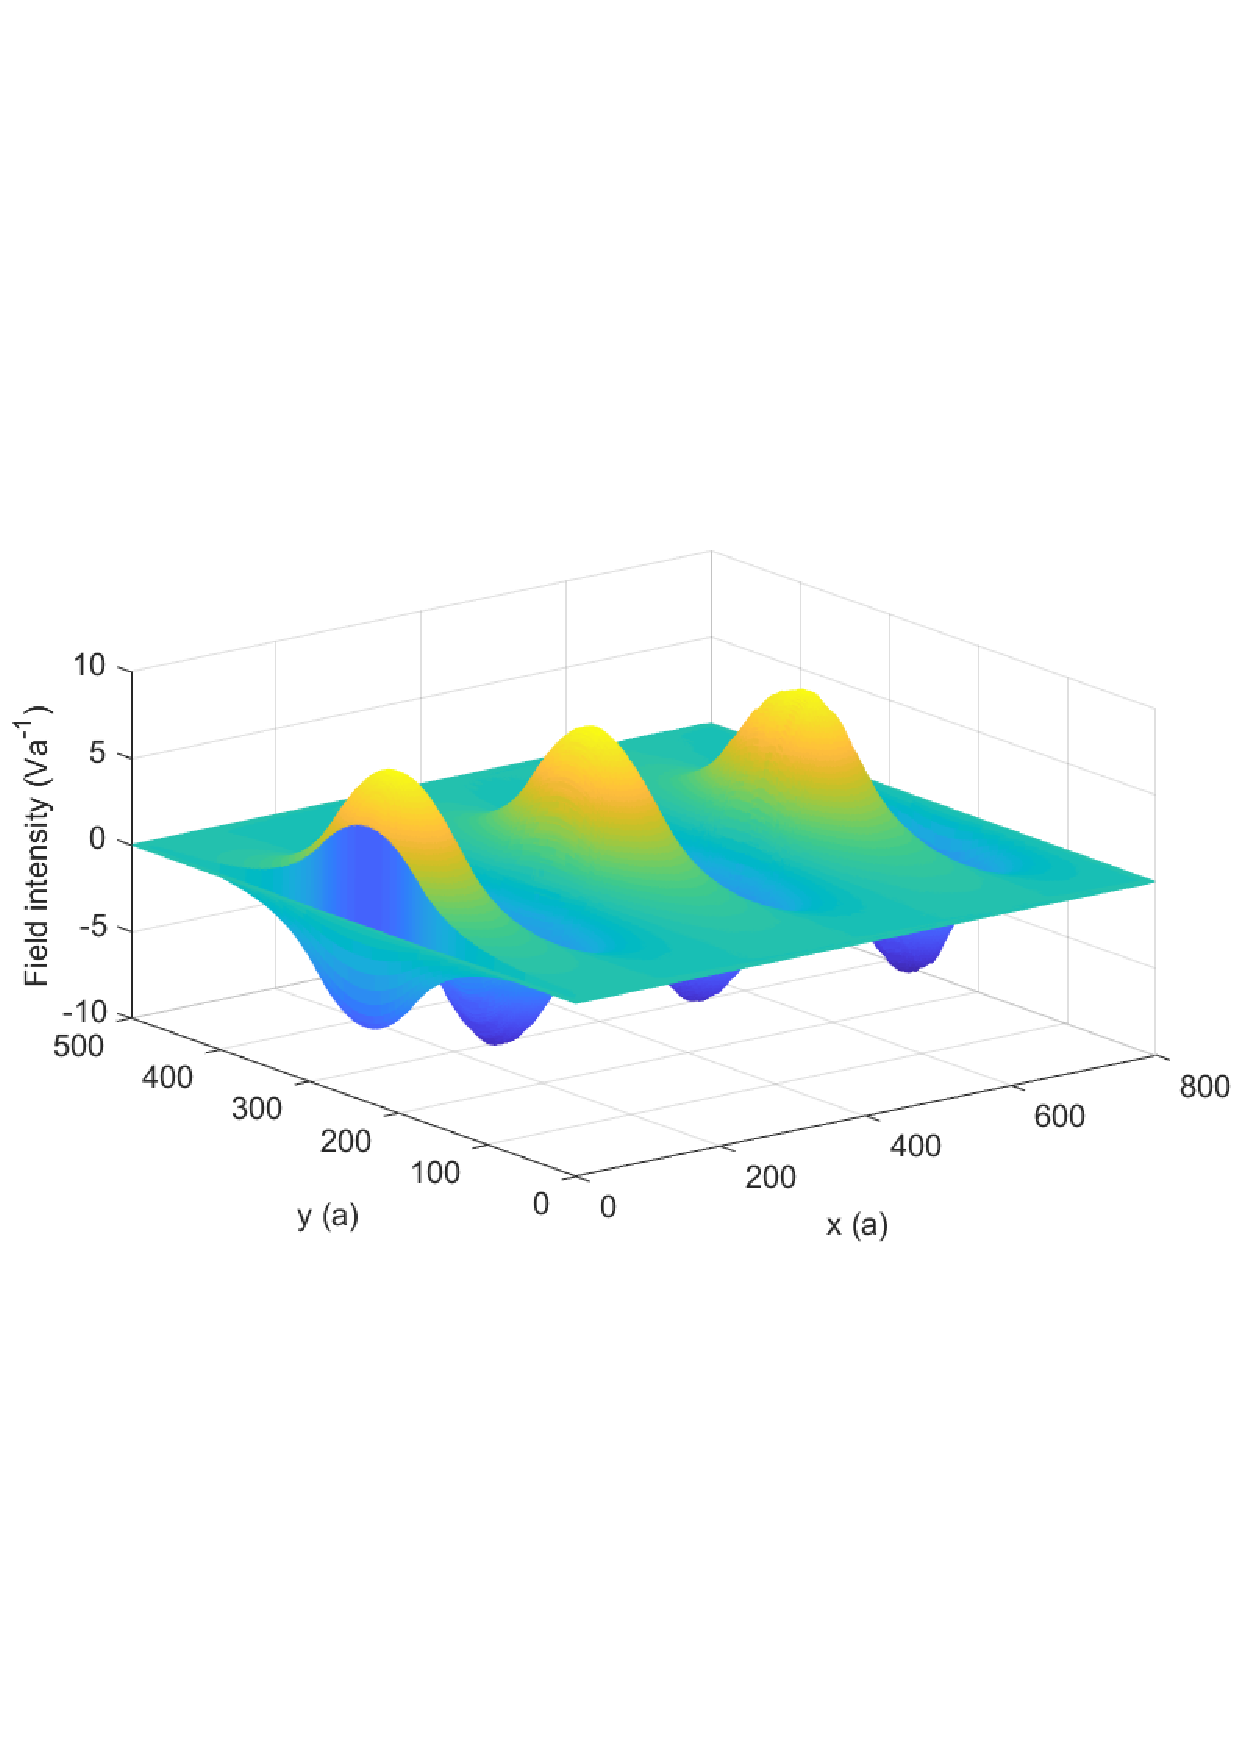
\includegraphics[trim={0 7cm 0 7cm}, scale=0.6]{graphs/modes/untitled.pdf}
	\caption[First two TE modes of a slab dielectric]{$3D$ representation of the electric $E_z$ field profile for mode $\ket{1}$. The excitation of the first fundamental mode is seen at $20 a$. $a$ is a variable length that can be adjusted to scale the entire simulation.}
	\label{fig:3dmode}
\end{figure}


\section{Demonstration of direct photonic transitions}

Here, a direct mode conversion is demonstrated through \textit{FDTD}. The waveguide is chosen to be of length $23 \mu m$ and width $1.1 \mu m$. From the previous band structure calculations, the mode $\ket{1}$ is known to exist at a frequency $\omega_1 = 0.129 (2 \pi c/a)$, and $\ket{2}$ at $\omega_2 = 0.199 (2 \pi c/a)$. Modulation is carried out from ... to ... The spatial discretisation is chosen as $\Delta x = \Delta y = 0.04$. A detector ($D_1$)is placed at $22 \mu m$ to collect the incident field after modulation, and another detector placed in the region between the source and the beginning of modulation($D_2$). To ensure the steady state solution is reached, the simulation is run for $10 000$ time steps. The results are shown in figure \ref{fig:reciprocalmode}. Importantly, we observe perfect mode conversion agreeing with the expected theory. The Fourier transform of the detector outputs illustrates the input $\ket{1}$ mode at $\omega_1 = 0.129 (2\pi c/a)$ and output in mode $\ket{2}$ at $\omega_2 = 0.199 (2\pi c/a)$. Additionally, a weak higher order mode $\ket{3}$ is observed at frequency $\omega_3 = 0.269 (2\pi c/a)$ in the output. The existence of the higher order mode is attributed to a further direct transition of the 2nd mode. 

\begin{figure}[t]
	\centering
	\setlength{\figH}{0.4\textwidth}
	\setlength{\figW}{0.7\textwidth}
	% This file was created by matlab2tikz.
%
%The latest updates can be retrieved from
%  http://www.mathworks.com/matlabcentral/fileexchange/22022-matlab2tikz-matlab2tikz
%where you can also make suggestions and rate matlab2tikz.
%
\definecolor{mycolor1}{rgb}{0.00000,0.44700,0.74100}%
\definecolor{mycolor2}{rgb}{0.85000,0.32500,0.09800}%
%
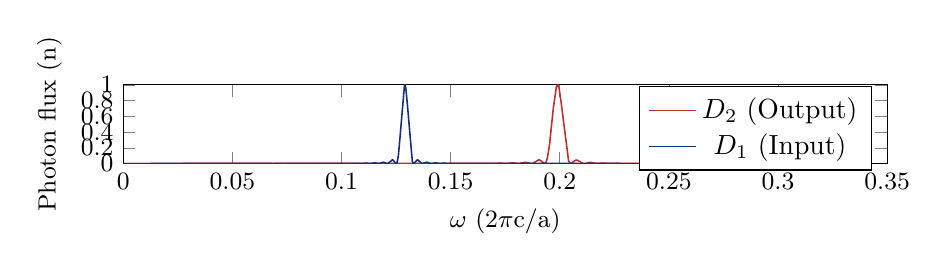
\begin{tikzpicture}

\begin{axis}[%
width=0.8\figW,
height=0.25\figH,
at={(0\figW,0\figH)},
scale only axis,
xmin=0,
yticklabel style={/pgf/number format/fixed},
xticklabel style={/pgf/number format/fixed},
xmax=0.35,
xlabel={$\omega\text{ (2}\pi\text{c/a)}$},
ymin=0,
ymax=1,
ylabel={Photon flux (n)},
axis background/.style={fill=white}
]
\addplot [color=mode2, line width = 0.2mm]
  table[row sep=crcr]{%
0	6.90869460877597e-05\\
0.117304596739771	0.000462718159760289\\
0.125978998091404	0.000297382378737554\\
0.128180961511434	0.000352644284727033\\
0.132184531366034	0.00136759188320346\\
0.135987922727904	0.000623862971118383\\
0.139057326283097	0.000828198409184244\\
0.141859825181316	0.000660951377172703\\
0.144595597915293	0.000880803909467209\\
0.147264644485026	0.000661010805538709\\
0.149933691054759	0.00104813172839613\\
0.152602737624492	0.000634754192933906\\
0.155471962686955	0.00129608157213545\\
0.158074283092445	0.000596691713695474\\
0.161210412811882	0.00169181178897571\\
0.163679280888885	0.000537857283981813\\
0.165080530337995	0.00187689072933561\\
0.166348327458618	0.00275244484186965\\
0.167349219922268	0.00209827972595544\\
0.169217552521081	0.000402898721760359\\
0.170151718820488	0.00130727836939815\\
0.172286956076274	0.00435614718142729\\
0.173154396211437	0.0034196358130536\\
0.175089454974494	0.00033783528024256\\
0.175823442781171	0.00131201058789543\\
0.178292310858174	0.00759803878669318\\
0.179026298664851	0.0062312771917945\\
0.18102808359215	0.00027904961622327\\
0.18162861907034	0.00151927091309956\\
0.182562785369747	0.0071249763018022\\
0.184097487147343	0.0157152582445836\\
0.18463129646129	0.0151205659351976\\
0.185365284267967	0.0106805311974563\\
0.186966712209806	0.000217090110192109\\
0.18743379535951	0.00173028610106374\\
0.1880343308377	0.0084738673201854\\
0.19043647275046	0.0469296521087703\\
0.19083682973592	0.0445060834473012\\
0.191504091378353	0.0318423586778283\\
0.192972066991706	0.000166588713402138\\
0.193238971648679	0.00213547272719938\\
0.193639328634139	0.0146414049227928\\
0.194306590276573	0.0681609150338081\\
0.195240756575979	0.223097752723171\\
0.197042363010549	0.699960097651519\\
0.198443612459659	0.97368804999049\\
0.198977421773606	1\\
0.199244326430579	0.993817527270956\\
0.199711409580282	0.952638619245898\\
0.200578849715445	0.788690155144477\\
0.204048610256099	0.0333279927147885\\
0.204849324227019	0.000948272372751857\\
0.205049502719749	0.000118381422221425\\
0.205383133540965	0.00313178746896159\\
0.206250573676128	0.0239506141498314\\
0.207384918468265	0.0440519518109421\\
0.207585096960995	0.0445989555779434\\
0.207985453946455	0.0428311430828778\\
0.208652715588888	0.0331925278406733\\
0.210721226680431	0.00079239642971829\\
0.211054857501648	9.47016444752258e-05\\
0.211588666815595	0.00170767127777194\\
0.213790630235625	0.0144060916740212\\
0.214391165713814	0.0130535901147792\\
0.215525510505951	0.00602516654503416\\
0.216726581462331	0.000416984425901878\\
0.217260390776278	0.000189870516005719\\
0.217994378582954	0.0018535808012381\\
0.219729258853281	0.00651767931620006\\
0.220463246659957	0.00597110525495781\\
0.221797769944824	0.00218566643168572\\
0.222932114736961	0.000164174141741524\\
0.223732828707881	0.00057208555282684\\
0.226068244456397	0.00343010723270276\\
0.227069136920047	0.00243806872616137\\
0.22893746951886	0.000187253079213079\\
0.230005088146753	0.000596664568742744\\
0.232006873074053	0.00195118002163341\\
0.233274670194676	0.00126137393949266\\
0.235076276629246	0.00020982260593283\\
0.236610978406843	0.000746757395190256\\
0.238279132512926	0.00113072027948724\\
0.242416154696012	0.000484357236604227\\
0.244618118116042	0.000657299140288004\\
0.248087878656696	0.000384430844256878\\
0.251424186868862	0.000368964292266183\\
0.258296981785925	0.000433298881798105\\
0.261166206848388	0.000634423609358281\\
0.263501622596904	0.000373648648806624\\
0.264569241224798	0.0015449099263416\\
0.265837038345421	0.00477866594844389\\
0.268639537243641	0.0126852117739487\\
0.269440251214561	0.0126759087932213\\
0.270374417513967	0.0109087311214555\\
0.274511439697054	0.000264945650912729\\
0.275779236817677	0.000339848587029845\\
0.277914474073463	0.000734609053077762\\
0.282118222420793	0.000296144777373719\\
0.28465381666204	0.000269904006837685\\
0.287523041724503	0.000192366491871265\\
0.290525719115452	0.000207772302890374\\
0.293461670342159	0.000173096362881653\\
0.296464347733109	0.000200634199863048\\
0.299533751288302	0.000165982888722382\\
0.302669881007738	0.000170916018330081\\
0.305872736891418	0.000176753006553287\\
0.309275771267828	9.51751238431608e-05\\
0.31594838769216	4.70114322019821e-05\\
0.333564095052399	5.21973813545351e-05\\
};
\addlegendentry{$D_2$ (Output)}

\addplot [color=mode1, line width = 0.2mm]
  table[row sep=crcr]{%
0	9.84499576692777e-05\\
0.0667261642433286	0.000428427228356787\\
0.068661223006385	6.13305372691997e-05\\
0.0702626509482249	0.000374831456357638\\
0.0717306265615782	0.000351368916442052\\
0.0734655068319048	0.000123256754796186\\
0.0755340179234478	0.000487187979007375\\
0.0774690766865045	0.000131415964435666\\
0.0794708616138042	0.000583041003948681\\
0.0814059203768609	0.000123277227918717\\
0.0834744314684039	0.000702983462822937\\
0.0853427640672171	0.000109068278802305\\
0.0874780013230037	0.000831396473917945\\
0.0893463339218168	0.000121856262543352\\
0.0914148450133601	0.00105879897365746\\
0.0933499037764167	0.000146538997274126\\
0.0954184148679598	0.00133377399004853\\
0.0973534736310164	0.000164486871907288\\
0.0994219847225595	0.00167874640134524\\
0.101290317321373	0.000160923180471562\\
0.102558114441996	0.00216389097464975\\
0.103292102248673	0.00241524257214309\\
0.105227161011729	0.000129803064990774\\
0.106094601146892	0.00184495690976028\\
0.107095493610542	0.00341718315492523\\
0.107829481417219	0.00230563928595595\\
0.109030552373599	3.30608605381144e-05\\
0.109697814016032	0.00127003609093057\\
0.111099063465142	0.00515347101819752\\
0.111699598943332	0.00401678469918942\\
0.113034122228199	4.04586502038562e-05\\
0.113567931542145	0.00134799796618279\\
0.115102633319742	0.00850395286559102\\
0.115569716469445	0.00743269865808505\\
0.117037692082798	3.74847521795729e-05\\
0.117438049068258	0.00142940397848035\\
0.118172036874935	0.00887593076299287\\
0.119172929338585	0.0165955252138328\\
0.119573286324045	0.0148584893668855\\
0.120507452623451	0.00318449807704857\\
0.120974535773155	3.8371287889083e-05\\
0.121308166594371	0.00168441406063069\\
0.121841975908318	0.0122478495686607\\
0.123309951521671	0.0479045978139261\\
0.123643582342888	0.0439487047529896\\
0.124310843985321	0.0199913970337922\\
0.124978105627754	7.54562746287935e-05\\
0.125178284120484	0.0021059847279834\\
0.125511914941701	0.0202086890353097\\
0.126045724255648	0.0992294441321038\\
0.126913164390811	0.370292542497138\\
0.128848223153867	0.995328829661499\\
0.128981675482354	1\\
0.129115127810841	0.997360946624525\\
0.129448758632057	0.959402049129023\\
0.130116020274491	0.769030373043881\\
0.132451436023007	0.0240565336073533\\
0.132985245336954	4.48384782758549e-05\\
0.133252149993927	0.00335261462704084\\
0.13472012560728	0.0467472013009338\\
0.134987030264254	0.0448349887504631\\
0.135587565742444	0.0297499812744499\\
0.136855362863067	0.000366988704898708\\
0.13732244601277	0.00146520772117942\\
0.138857147790367	0.0163715424299369\\
0.139257504775827	0.0147236468621543\\
0.140992385046153	2.33173488148886e-05\\
0.141459468195857	0.00125620832661566\\
0.14292744380921	0.00815906522325061\\
0.143461253123156	0.00666437845181656\\
0.145062681064996	3.97393674484992e-05\\
0.145663216543186	0.00141873686971694\\
0.146931013663809	0.0049064410312829\\
0.147598275306243	0.0036444960007358\\
0.148999524755353	2.07389463589003e-05\\
0.149666786397786	0.000949168867018013\\
0.151001309682653	0.0033086037718042\\
0.151735297489329	0.00219941722131867\\
0.153003094609952	2.31696749273258e-05\\
0.153803808580872	0.000875541856105944\\
0.155004879537252	0.0022946879878436\\
0.155939045836659	0.00118502317076197\\
0.157006664464552	2.50932747978272e-05\\
0.157940830763959	0.000870234729765329\\
0.159008449391852	0.00175351556770953\\
0.160009341855502	0.000822553119057101\\
0.161076960483395	2.5835821583664e-05\\
0.162278031439775	0.00100985651658969\\
0.163278923903425	0.00127677268050475\\
0.165480887323455	0.000174831306815948\\
0.167282493758025	0.00100268275262039\\
0.169484457178054	0.000154362218679482\\
0.171286063612624	0.000837581992396252\\
0.173554753196898	0.000156493639497102\\
0.175356359631467	0.000664462792619336\\
0.177558323051497	0.000139270865808117\\
0.17942665565031	0.00054846371981343\\
0.181561892906097	0.000129298783461129\\
0.183496951669153	0.000454102606039175\\
0.18563218892494	0.000138974956166438\\
0.187567247687996	0.000371353963459331\\
0.18963575877954	0.000127635902729795\\
0.191770996035326	0.000327556641592119\\
0.193839507126869	0.000284120381486952\\
0.198310160131172	0.00147711410892404\\
0.199511231087552	0.00162237441253588\\
0.202980991628205	0.000349764060434188\\
0.209787060381025	0.000112369158659753\\
0.212189202293785	9.03789330184424e-05\\
0.214658070370788	0.000213182953904933\\
0.256028292201651	4.36960900880301e-05\\
0.264235610403581	1.15791841748258e-05\\
0.272576380933997	7.78270854289165e-05\\
0.27564578448919	0.000118218973406359\\
0.282184948585036	5.81626725664197e-05\\
0.288056851038449	4.09973175865552e-05\\
0.297865597182219	2.1872373606513e-05\\
0.308475057296908	1.79951008263401e-05\\
0.32595731232866	2.24253517078221e-05\\
0.333564095052399	1.44925264395912e-05\\
};
\addlegendentry{$D_1$ (Input)}
\end{axis}
\end{tikzpicture}%
	\caption[The modulated waveguide structure]{LR 12.25 and width 1.1}
	\label{fig:reciprocalmode_fourier}
\end{figure} 

\begin{figure}[t]
	\centering
	\setlength{\figH}{0.1\textwidth}
	\setlength{\figW}{0.8\textwidth}
	% This file was created by matlab2tikz.
%
%The latest updates can be retrieved from
%  http://www.mathworks.com/matlabcentral/fileexchange/22022-matlab2tikz-matlab2tikz
%where you can also make suggestions and rate matlab2tikz.
%
\begin{tikzpicture}

\begin{axis}[%
width=0.8\figW,
height=0.1\figH,
at={(0,0\figH)},
scale only axis,
point meta min=-0.348002718984685,
point meta max=0.348002718984685,
axis on top,
xmin=0,
xmax=23,
xlabel style={font=\color{white!15!black}},
xlabel={$\text{x (}\mu\text{m)}$},
ymin=0,
ymax=5,
ylabel style={font=\color{white!15!black}},
ylabel={$\text{y (}\mu\text{m)}$},
axis background/.style={fill=white},
colormap={mymap}{[1pt] rgb(0pt)=(0,0,1); rgb(31pt)=(1,1,1); rgb(32pt)=(1,1,1); rgb(63pt)=(1,0,0)},
colorbar,
colorbar style={width=.01\linewidth, at={(1.03,0.1\figH)}}
]
\addplot graphics [xmin=0, xmax=23, ymin=0, ymax=5] {graphs/fdtd/reciprocal/LR-1.png};
\draw (0,1.95) -- (23,1.95);
\draw (0,3.05) -- (23,3.05);
\end{axis}
\node[below right]
at (current bounding box.north west) {\textbf{a}};
\end{tikzpicture}%
	\caption[The modulated waveguide structure]{LR 12.25 and width 1.1}
	\label{fig:reciprocalmode}
\end{figure} 

We can further detect the amplitude of each mode while it is undergoing modulation by placing an array of probes in the modulation region ($2 \mu m$ to $21 \mu m$).

\begin{figure}[t]
	\centering
	\setlength{\figH}{0.3\textwidth}
	\setlength{\figW}{0.8\textwidth}
	% This file was created by matlab2tikz.
%
%The latest updates can be retrieved from
%  http://www.mathworks.com/matlabcentral/fileexchange/22022-matlab2tikz-matlab2tikz
%where you can also make suggestions and rate matlab2tikz.
%
\definecolor{mycolor1}{rgb}{0.00000,0.44706,0.74118}%
%
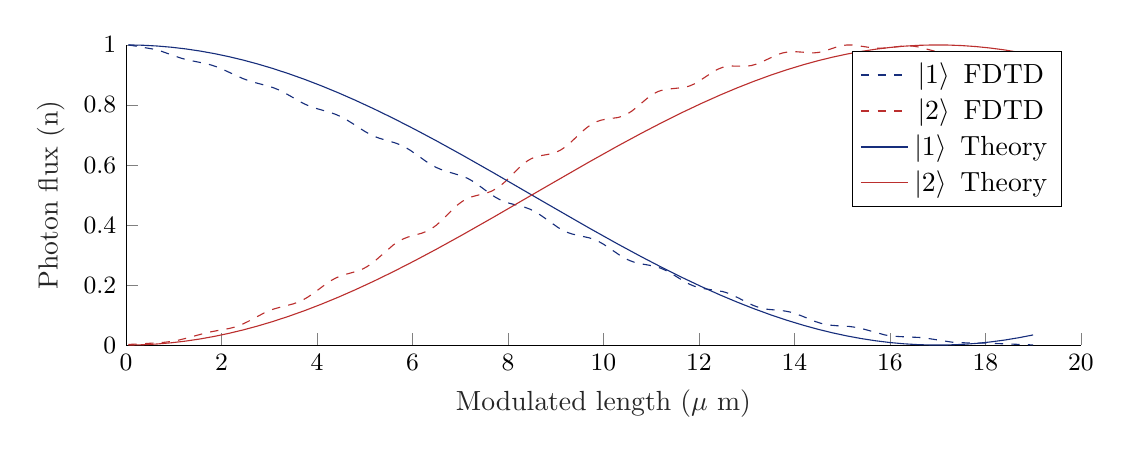
\begin{tikzpicture}

\begin{axis}[%
width=\figW,
height=0.953\figH,
at={(0\figW,0\figH)},
scale only axis,
xmin=0,
xmax=20,
xlabel style={font=\color{white!15!black}},
xlabel={$\text{Modulated length (}\mu\text{ m)}$},
ymin=0,
ymax=1,
ylabel style={font=\color{white!15!black}},
ylabel={Photon flux (n)},
axis background/.style={fill=white},
axis x line*=bottom,
axis y line*=left
]
\addplot [color=mode1, dashed]
  table[row sep=crcr]{%
0.0500000000000007	1\\
0.600000000000001	0.985300295000002\\
0.75	0.978307094000002\\
0.949999999999999	0.966962502000001\\
1.15	0.955967848\\
1.3	0.949529264999999\\
1.5	0.943224780000001\\
1.7	0.936686416000001\\
1.8	0.932249582000001\\
1.9	0.926748569000001\\
2.05	0.916703029000001\\
2.45	0.887680901\\
2.6	0.879206137000001\\
2.75	0.872444712\\
3	0.861921154000001\\
3.1	0.856601853000001\\
3.2	0.850093187999999\\
3.3	0.842329978999999\\
3.45	0.828904319999999\\
3.65	0.810516472\\
3.75	0.802424972000001\\
3.85	0.795547412000001\\
3.95	0.789883003\\
4.15	0.780810902999999\\
4.3	0.773791525\\
4.4	0.767991468000002\\
4.5	0.760904049000001\\
4.6	0.752460313\\
4.75	0.737729229999999\\
5	0.711972104000001\\
5.1	0.703014224\\
5.2	0.69547489\\
5.3	0.689397643\\
5.45	0.68227298\\
5.65	0.672930932\\
5.75	0.666709385000001\\
5.85	0.658846894\\
5.95	0.649328528000002\\
6.1	0.632793121999999\\
6.3	0.610139072999999\\
6.4	0.600146723000002\\
6.5	0.59167617\\
6.6	0.584833270000001\\
6.7	0.579401854\\
7.05	0.562789358\\
7.15	0.555824682000001\\
7.25	0.547066998000002\\
7.35	0.536633309999999\\
7.5	0.519017741999999\\
7.65	0.501544104000001\\
7.75	0.491357915999998\\
7.85	0.482975941999999\\
7.95	0.476501292999998\\
8.05	0.471621516999999\\
8.35	0.459346862\\
8.45	0.453445923\\
8.55	0.445793471000002\\
8.65	0.436371911999998\\
8.75	0.425522733000001\\
9.05	0.391544724999999\\
9.15	0.382366125000001\\
9.25	0.375122797\\
9.35	0.369789205\\
9.5	0.364313612\\
9.7	0.357361956999998\\
9.8	0.352131846999999\\
9.9	0.345060586999999\\
10	0.336144098999998\\
10.15	0.320269456999998\\
10.35	0.298483525000002\\
10.45	0.289129591999998\\
10.55	0.281529978000002\\
10.65	0.275823152000001\\
10.75	0.271776965000001\\
10.95	0.266245011999999\\
11.1	0.261211905\\
11.2	0.256117153000002\\
11.3	0.249257267000001\\
11.4	0.240749382000001\\
11.55	0.226045947999999\\
11.7	0.211409891999999\\
11.8	0.203010402\\
11.9	0.196317837999999\\
12	0.191464149000002\\
12.1	0.1882071\\
12.5	0.178297374\\
12.6	0.173413256\\
12.7	0.167016173\\
12.85	0.155226093\\
13.05	0.138578878000001\\
13.15	0.131404347\\
13.25	0.125685127000001\\
13.35	0.121594976000001\\
13.45	0.118974524999999\\
13.65	0.116139087000001\\
13.8	0.113498306\\
13.9	0.110441199\\
14	0.106067648\\
14.15	0.0973283850000009\\
14.45	0.0778342189999996\\
14.55	0.0727266610000008\\
14.65	0.0688917290000006\\
14.75	0.0663358810000005\\
14.9	0.0643367770000012\\
15.15	0.0620220469999992\\
15.3	0.058759417000001\\
15.45	0.0533310030000003\\
15.9	0.0336135750000004\\
16.05	0.0299902209999985\\
16.2	0.0283199590000009\\
16.65	0.0251553320000006\\
16.8	0.0220658510000007\\
17.3	0.00971707300000091\\
17.45	0.00799669499999922\\
17.65	0.00725801999999831\\
18.05	0.0062111420000015\\
18.95	0.000810164000000668\\
19	0.0007589579999987\\
};
\addlegendentry{$\ket{1}\text{ FDTD}$}

\addplot [color=mode2, dashed]
  table[row sep=crcr]{%
0.0500000000000007	0.00216580500000063\\
0.300000000000001	0.00389339199999839\\
0.800000000000001	0.00923097700000142\\
0.949999999999999	0.0120812470000011\\
1.1	0.0164435689999998\\
1.25	0.0223303679999987\\
1.7	0.0417885349999985\\
1.9	0.047863177\\
2.15	0.0548989800000008\\
2.25	0.0587970210000002\\
2.35	0.0638805620000014\\
2.45	0.0703077289999996\\
2.6	0.0821650920000003\\
2.9	0.107745329\\
3	0.114738200000001\\
3.1	0.120460883\\
3.25	0.127062223999999\\
3.5	0.137206189\\
3.6	0.142823344\\
3.7	0.150052496000001\\
3.8	0.159038304999999\\
3.9	0.169611783000001\\
4.05	0.187336919\\
4.2	0.204989429000001\\
4.3	0.215366144000001\\
4.4	0.223950427999998\\
4.5	0.230592865999999\\
4.6	0.235612417999999\\
4.85	0.246540120999999\\
4.95	0.252889925000002\\
5.05	0.261470484\\
5.15	0.272419852999999\\
5.25	0.285375354999999\\
5.6	0.333812644999998\\
5.7	0.344697831000001\\
5.8	0.353268869000001\\
5.9	0.359647155000001\\
6.05	0.366451613999999\\
6.2	0.373044146000002\\
6.3	0.379229246000001\\
6.4	0.387904595999998\\
6.5	0.399429082000001\\
6.6	0.413532834000002\\
6.75	0.437494039000001\\
6.85	0.453401125999999\\
6.95	0.467697244\\
7.05	0.479428260999999\\
7.15	0.488220944999998\\
7.25	0.494349708000001\\
7.35	0.498636414\\
7.55	0.506436509\\
7.65	0.512325863000001\\
7.75	0.520696685000001\\
7.85	0.531867519999999\\
7.95	0.545624877000002\\
8.05	0.561237255000002\\
8.25	0.593218749999998\\
8.35	0.606909778999999\\
8.4	0.612688882\\
8.45	0.617679139\\
8.5	0.621834007\\
8.6	0.627836250000001\\
8.7	0.631446724\\
8.9	0.636969961999998\\
9	0.64182254\\
9.1	0.649443315999999\\
9.2	0.660075018000001\\
9.3	0.673288244999998\\
9.45	0.695772791\\
9.55	0.710720397999999\\
9.65	0.724234045999999\\
9.75	0.735409001000001\\
9.85	0.743758795000002\\
9.95	0.749293149\\
10.05	0.752544454999999\\
10.3	0.757980238000002\\
10.4	0.762524254999999\\
10.5	0.769885389999999\\
10.6	0.780218057999999\\
10.7	0.792930987999998\\
10.95	0.826663398000001\\
11.05	0.837340602000001\\
11.15	0.845143547999999\\
11.25	0.850075296\\
11.35	0.852711616000001\\
11.7	0.858467137000002\\
11.8	0.863036862000001\\
11.9	0.869857451000001\\
12	0.878796755\\
12.15	0.894789954\\
12.3	0.910713691000002\\
12.4	0.919354812000002\\
12.5	0.925425657000002\\
12.6	0.928702482999999\\
12.7	0.929620229000001\\
13	0.929041353999999\\
13.1	0.931378328000001\\
13.2	0.935854369000001\\
13.3	0.942194992000001\\
13.65	0.967952771\\
13.75	0.973048064\\
13.85	0.976240560000001\\
13.95	0.977506353999999\\
14.05	0.977141171\\
14.4	0.973388779\\
14.5	0.974887964000001\\
14.6	0.978254222\\
14.75	0.985860002999999\\
14.9	0.993843981000001\\
15	0.997743261\\
15.1	0.999751747000001\\
15.2	0.999763796\\
15.3	0.998142525999999\\
15.65	0.989724817999999\\
15.75	0.988928892000001\\
15.85	0.989228392000001\\
16	0.991365311999999\\
16.3	0.996693215000001\\
16.4	0.996914953000001\\
16.5	0.995687951000001\\
16.6	0.992986132999999\\
16.75	0.986996400999999\\
16.9	0.980768823000002\\
17	0.977677851999999\\
17.1	0.975866584999999\\
17.25	0.975143640999999\\
17.45	0.974702435000001\\
17.55	0.973245497000001\\
17.65	0.970560638999999\\
17.8	0.964533818\\
18.25	0.943732929999999\\
18.4	0.938714709999999\\
18.6	0.933800534\\
18.75	0.930079806999998\\
18.85	0.926607670999999\\
18.95	0.921850465999999\\
19	0.918948554\\
};
\addlegendentry{$\ket{2}\text{ FDTD}$}

\addplot [color=mode1]
  table[row sep=crcr]{%
0.0500000000000007	0.999978656\\
0.350000000000001	0.998954493999999\\
0.649999999999999	0.996397148\\
0.949999999999999	0.992314478000001\\
1.25	0.986719026999999\\
1.55	0.979627990000001\\
1.85	0.971063156\\
2.15	0.961050842999999\\
2.45	0.949621816000001\\
2.75	0.936811195000001\\
3.05	0.922658343999998\\
3.4	0.904508496999998\\
3.75	0.884666984999999\\
4.1	0.863216786999999\\
4.45	0.840247606999998\\
4.8	0.815855503000002\\
5.2	0.786367569999999\\
5.6	0.755315596999999\\
6.05	0.718724078000001\\
6.5	0.680620832999999\\
7.05	0.632382093\\
7.7	0.573650849\\
8.8	0.472294262999998\\
9.7	0.390026820999999\\
10.3	0.336730643999999\\
10.8	0.293821841\\
11.25	0.256697761000002\\
11.65	0.225102566\\
12.05	0.195008766000001\\
12.45	0.166580721999999\\
12.8	0.143194922999999\\
13.15	0.121301291000002\\
13.5	0.100991386\\
13.85	0.0823501459999996\\
14.2	0.065455527000001\\
14.5	0.0524183540000003\\
14.8	0.0407565070000011\\
15.1	0.0305058199999984\\
15.4	0.021697790000001\\
15.7	0.0143594839999999\\
16	0.00851344999999881\\
16.3	0.0041776519999992\\
16.6	0.00136541299999848\\
16.9	8.53748000011478e-05\\
17.2	0.000341469999998623\\
17.5	0.00213291200000043\\
17.8	0.00545419599999875\\
18.1	0.0102951160000018\\
18.4	0.016640798000001\\
18.7	0.0244717419999994\\
19	0.0337638849999991\\
};
\addlegendentry{$\ket{1}\text{ Theory}$}

\addplot [color=mode2]
  table[row sep=crcr]{%
0.0500000000000007	2.13440999985437e-05\\
0.350000000000001	0.00104550600000053\\
0.649999999999999	0.00360285200000021\\
0.949999999999999	0.00768552199999917\\
1.25	0.0132809730000005\\
1.55	0.0203720099999991\\
1.85	0.0289368440000004\\
2.15	0.0389491570000011\\
2.45	0.0503781839999995\\
2.75	0.0631888049999993\\
3.05	0.0773416560000015\\
3.4	0.0954915030000016\\
3.75	0.115333015000001\\
4.1	0.136783213000001\\
4.45	0.159752393000002\\
4.8	0.184144496999998\\
5.2	0.213632430000001\\
5.6	0.244684403000001\\
6.05	0.281275921999999\\
6.5	0.319379167000001\\
7.05	0.367617907\\
7.7	0.426349151\\
8.8	0.527705737000002\\
9.7	0.609973179000001\\
10.3	0.663269356000001\\
10.8	0.706178159\\
11.25	0.743302238999998\\
11.65	0.774897434\\
12.05	0.804991233999999\\
12.45	0.833419278000001\\
12.8	0.856805077000001\\
13.15	0.878698709000002\\
13.5	0.899008614\\
13.85	0.917649854\\
14.2	0.934544472999999\\
14.5	0.947581646\\
14.8	0.959243492999999\\
15.1	0.969494180000002\\
15.4	0.978302209999999\\
15.7	0.985640516\\
16	0.991486550000001\\
16.3	0.995822348000001\\
16.6	0.998634587000002\\
16.9	0.999914624999999\\
17.2	0.999658530000001\\
17.5	0.997867088\\
17.8	0.994545804000001\\
18.1	0.989704884000002\\
18.4	0.983359201999999\\
18.7	0.975528258000001\\
19	0.966236115000001\\
};
\addlegendentry{$\ket{2}\text{ Theory}$}

\end{axis}
\end{tikzpicture}%
	\caption[The modulated waveguide structure]{LR 12.25 and width 1.1}
	\label{fig:coherencelength}
\end{figure} 


\begin{figure}[t]
\centering
\setlength{\figH}{1\textwidth}
\setlength{\figW}{1\textwidth}
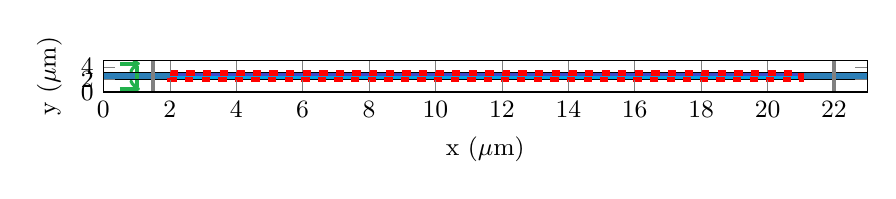
\begin{tikzpicture}
    \begin{axis}[%
width=0.8\figW,
height=0.1\figH,
at={(0\figW,0\figH)},
scale only axis,
axis on top,
xmin=0,
xmax=23,
xlabel={$\text{x (}\mu\text{m)}$},
ymin=0,
ymax=5,
ylabel={$\text{y (}\mu\text{m)}$},
axis background/.style={fill=white},
]
\fill[fill=eps] (0,1.95) rectangle (23,3.05);
\fill[fill=epsilon] (2,2.5) rectangle (21,3.05);
\fill[fill=modup] (2,2.5) rectangle (21,1.95);
\draw[draw=src, line width=0.5mm] (1,0.8) -- (1,4.2);
\draw[line width=0.5mm, draw=src, ->] (0.5,4.5) -- (1.1,4.5);
\draw[line width=0.5mm, draw=src, ->] (0.5,0.5) -- (1.1,0.5);
%\draw[pattern=north west lines, pattern color=black] (0,0) rectangle (60,0.5);
%\draw[pattern=north west lines, pattern color=black] (0,0) rectangle (0.5,5);
%\draw[pattern=north west lines, pattern color=black] (0,5) rectangle (60,4.5);
%\draw[pattern=north west lines, pattern color=black] (60,0) rectangle (59.5,4.5);
\draw (0,1.95) -- (24.2,1.95) -- (24.2,1.5) -- (35.8,1.5) -- (35.8,1.95) -- (60,1.95);
\draw (0,3.05) -- (24.2,3.05) -- (24.2,3.5) -- (35.8,3.5) -- (35.8,3.05) -- (60,3.05);
\draw[draw=red, dashed, line width=0.7mm] (2,3.05) -- (21,3.05) -- (21,1.95) -- (2,1.95) -- (2,3.05);
\draw[draw=gray, line width = 0.5mm] (1.5,0) -- (1.5,5);
\draw[draw=gray, line width = 0.5mm] (22,0) -- (22,5);
\end{axis}
\end{tikzpicture}
\caption[The modulated waveguide structure]{The modulated waveguide structure. The dark blue region is a material of unity permeability and permittivity of $\epsilon_{wg} = 12.25$. The light blue sections are regions where the permittivity is modulated by an amount $0.1 \epsilon_{wg} \cos(\omega t + \phi)$, with $\phi=0$ on the left and $\phi=\frac{\pi}{2}$ on the right. The modulation region is chosen to only cover the upper half of the waveguide to maximise the coupling. The diagonal lines around the edges represent the \textit{PML} layer, marking the point where the fields effectively decay to zero. Note that the layer width is constant across the \textit{x} and \textit{y} directions. The red line indicates the region over which the modal source is injected, in this case, from left to right (LR).}
\label{fig:cavity}
\end{figure} 

\subsection{Phase-matched non-reciprocal propagation}
width 0.22, eps 12.25

\begin{figure}[t]
	\centering
	\setlength{\figH}{0.4\textwidth}
	\setlength{\figW}{0.7\textwidth}
	% This file was created by matlab2tikz.
%
%The latest updates can be retrieved from
%  http://www.mathworks.com/matlabcentral/fileexchange/22022-matlab2tikz-matlab2tikz
%where you can also make suggestions and rate matlab2tikz.
%
%
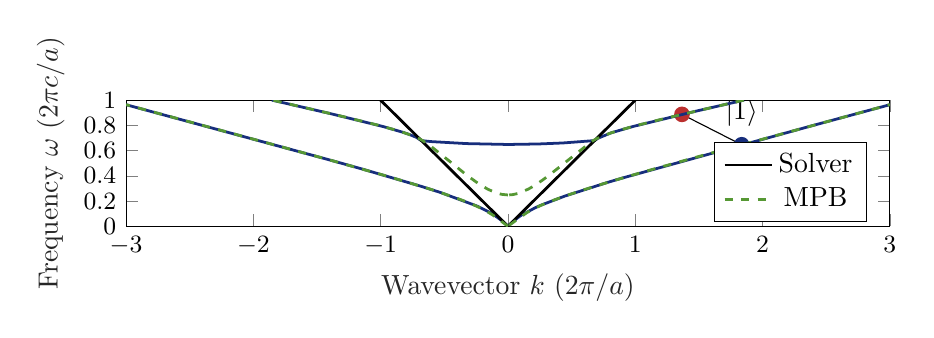
\begin{tikzpicture}

\begin{axis}[%
width=0.8\figW,
height=0.4\figH,
at={(0\figW,0\figH)},
scale only axis,
xmin=-3,
xmax=3,
xlabel style={font=\color{white!15!black}},
xlabel={Wavevector $k$ ($2 \pi /a$)},
ymin=0,
ymax=1,
ylabel style={font=\color{white!15!black}},
ylabel={Frequency $\omega$ ($2\pi c/a$)},
axis background/.style={fill=white},
legend pos=south east
]
%\draw[dashed] (-3,0.6468) -- (3,0.6468);
%\draw[dashed] (-3,0.8879) -- (3,0.8879);
%\node at (2.8,0.767) {$\Omega$};
%\draw[dashed] (1.836,0.6468) -- (1.836,0);
%\draw[dashed] (1.367,0.8879) -- (1.367,0);
\draw[->] (1.836,0.6468) -- (1.367,0.8879);
\node[label={90:{$\ket{1}$}},circle,fill=mode1,inner sep=2pt] at (1.836,0.6468) {};
\node[label={90:{$\ket{2}$}},circle,fill=mode2,inner sep=2pt] at (1.367,0.8879) {};
%\node[label={180:{}},circle,fill=mode3,inner sep=2pt] at (-2.305,0.8879) {};
\addplot [color=mode1, forget plot, line width=1.0pt]
table[row sep=crcr]{%
	-0	0\\
	-0.0425483776636622	0.04\\
	-0.112747396858924	0.0920000000000001\\
	-0.138703575229707	0.108\\
	-0.242619225661566	0.16\\
	-0.530251013303014	0.268\\
	-0.68277422737238	0.317\\
	-1.13395473723024	0.451\\
	-1.40367460079584	0.527\\
	-3.00095872332965	0.965\\
};
\addlegendentry{Solver};
\addplot [color=mode1, forget plot, line width=1.0pt]
table[row sep=crcr]{%
	-0	0.649\\
	-0.326077818628705	0.656\\
	-0.605487195406852	0.672\\
	-0.681620546537656	0.68\\
	-0.720361604419702	0.706\\
	-0.780889623877291	0.731\\
	-0.822707823290201	0.745\\
	-0.979328562522052	0.791\\
	-1.40286353275794	0.896\\
	-1.58333534884432	0.938\\
	-1.73350139501897	0.973\\
	-1.85486453299797	1.001\\
};
\addplot [color=mode1, forget plot, line width=1.0pt]
  table[row sep=crcr]{%
0.00856527091199988	0.0089999999999999\\
0.0355740339675572	0.0329999999999999\\
0.0773642883861596	0.0680000000000001\\
0.108965071776361	0.0899999999999999\\
0.216446056096282	0.148\\
0.266469085354788	0.17\\
0.44579687604775	0.239\\
0.779460193245421	0.347\\
0.90346776025157	0.384\\
2.38185947042077	0.796\\
3.00095872332965	0.965\\
};
\addplot [color=mode1, forget plot, line width=1.0pt]
  table[row sep=crcr]{%
0	0.649\\
0.241290268767007	0.653\\
0.432426865263543	0.661\\
0.681620546537656	0.68\\
0.70634705751922	0.698\\
0.812185645324833	0.742\\
0.983207321695099	0.792\\
1.48370503209761	0.915\\
1.85486453299797	1.001\\
};
\addplot [name path=A, color=black, line width=1.0pt]
  table[row sep=crcr]{%
0.00996678000000006	0.00996678000000006\\
1.00664	1.00664\\
};
\addplot [color=mode3, dashed, line width=1.0pt]
  table[row sep=crcr]{%
0.00996678000000006	0.00783098999999998\\
0.149502	0.108661\\
0.199336	0.137065\\
0.259136	0.166038\\
0.33887	0.199306\\
0.448505	0.239874\\
0.598007	0.290189\\
0.797342	0.352394\\
1.07641	0.434535\\
1.48505	0.549875\\
3	0.965172\\
};
\addlegendentry{MPB};
\addplot [color=mode3, dashed, line width=1.0pt, forget plot]
  table[row sep=crcr]{%
0.00996678000000006	0.248465\\
0.0398670999999999	0.251399\\
0.0797342000000001	0.260564\\
0.159468	0.294355\\
0.209302	0.32355\\
0.269103	0.364287\\
0.33887	0.417217\\
0.657807	0.673008\\
0.697674	0.695525\\
0.747508	0.71813\\
0.807309	0.740237\\
0.89701	0.768316\\
1.02658	0.803978\\
1.22591	0.85408\\
1.85382	1.00166\\
};
\addplot [name path=B, line width=1.0pt, color=black]
  table[row sep=crcr]{%
0	0\\
-1.00664	1.00664\\
};

\addplot [color=mode3, dashed, forget plot, line width=1.0pt]
  table[row sep=crcr]{%
-0	0\\
-0.119601	0.0893928000000002\\
-0.199336	0.137065\\
-0.289037	0.179054\\
-0.418605	0.229214\\
-0.61794	0.296612\\
-0.92691	0.391046\\
-1.42525	0.533211\\
-2.51163	0.831749\\
-3	0.965172\\
};
\addplot [color=mode3, dashed, forget plot, line width=1.0pt]
  table[row sep=crcr]{%
-0	0.248268\\
-0.0498339000000001	0.253143\\
-0.0996678	0.267229\\
-0.159468	0.294355\\
-0.229236	0.336534\\
-0.318937	0.401633\\
-0.458472	0.515573\\
-0.627907	0.653101\\
-0.687708	0.690319\\
-0.757475	0.722111\\
-0.857143	0.756346\\
-1.02658	0.803978\\
-1.33555	0.880479\\
-1.85382	1.00166\\
};
\end{axis}



\end{tikzpicture}%
	\caption[]{}
	\label{fig:bandyu}
\end{figure} 

To determine the coherence length, we run the simulation for $15 \mu m$ and calculate the amplitudes of each mode along the length of modulation. Our design proposed here provides a $50 \%$ reduction in device footprint. By modulating each half of the wave guide with a $pi/2$ phase difference, the coherence length can be reduced drastically. To determine the coherence length, the simulation is run for an arbitrarily large modulation region and the amplitude of each mode is calculated at each point in the waveguide,

Our proposed device marks a $50 \%$ size reduction on previous phase matched structures, as the modulated structure is split with a $\pi/2$ phase difference.

LR:
\begin{figure}[t]
	\centering
	\setlength{\figH}{0.4\textwidth}
	\setlength{\figW}{0.8\textwidth}
	\begin{subfigure}[t]{0.5\textwidth}
	% This file was created by matlab2tikz.
%
%The latest updates can be retrieved from
%  http://www.mathworks.com/matlabcentral/fileexchange/22022-matlab2tikz-matlab2tikz
%where you can also make suggestions and rate matlab2tikz.
%
\begin{tikzpicture}

\begin{axis}[%
width=0.35\figW,
height=0.2\figH,
at={(0\figW,0.75\figW)},
scale only axis,
point meta min=-1,
point meta max=1,
axis on top,
clip=false,
xmin=0,
xmax=10,
ymin=0,
ymax=1,
xlabel = {x ($\mu m$)},
ytick={0,0.5,1},
yticklabels={$0$,$0.5$, $1$},
ylabel={$\text{y (}\mu\text{m)}$},
axis background/.style={fill=white},
colormap={mymap}{[1pt] rgb(0pt)=(0,0,1); rgb(31pt)=(1,1,1); rgb(32pt)=(1,1,1); rgb(63pt)=(1,0,0)},
colorbar,
colorbar style={width=.02\linewidth, at={(1.05,0.1\figH)}, anchor=east,ytick={-1,1}},
colorbar style={title={$V / \mu m$}}
]
\addplot graphics [xmin=0, xmax=10, ymin=0, ymax=1] {graphs/fdtd/phasematch/LR/field-1.png};
\node at (-1,2) {\textbf{(a)}};
\node at (2,1.2) {$\ket{1} \rightarrow$};
\node at (8,1.2) {$\rightarrow \ket{2}$};
\end{axis}

\begin{axis}[%
width=0.35\figW,
height=0.2\figH,
at={(0\figW,0.5\figW)},
scale only axis,
point meta min=-1,
point meta max=1,
axis on top,
xmin=0,
clip=false,
xmax=10,
ymin=0,
ymax=1,
xlabel = {x ($\mu m$)},
ytick={0,0.5,1},
yticklabels={$0$,$0.5$, $1$},
ylabel={$\text{y (}\mu\text{m)}$},
axis background/.style={fill=white},
colormap={mymap}{[1pt] rgb(0pt)=(0,0,1); rgb(31pt)=(1,1,1); rgb(32pt)=(1,1,1); rgb(63pt)=(1,0,0)},
colorbar,
colorbar style={width=.02\linewidth, at={(1.05,0.1\figH)}, anchor=east,ytick={-1,1}}
]
\addplot [forget plot] graphics [xmin=0, xmax=10, ymin=0, ymax=1] {graphs/fdtd/phasematch/RL/fieldRL-1.png};
\node at (-1,2) {\textbf{(b)}};
\node at (2,1.2) {$\bra{1} \leftarrow$};
\node at (8,1.2) {$\leftarrow \bra{1}$};
\end{axis}

\begin{axis}[%
width=0.35\figW,
height=0.2\figH,
at={(0\figW,0.25\figW)},
scale only axis,
point meta min=-1,
point meta max=1,
axis on top,
xmin=0,
xmax=10,
ymin=0,
ymax=1,
ytick={0,0.5,1},
clip=false,
xlabel = {x ($\mu m$)},
yticklabels={$0$,$0.5$, $1$},
ylabel={$\text{y (}\mu\text{m)}$},
axis background/.style={fill=white},
colormap={mymap}{[1pt] rgb(0pt)=(0,0,1); rgb(31pt)=(1,1,1); rgb(32pt)=(1,1,1); rgb(63pt)=(1,0,0)},
colorbar,
colorbar style={width=.02\linewidth, at={(1.05,0.1\figH)}, anchor=east,ytick={-1,1}}
]
\addplot [forget plot] graphics [xmin=0, xmax=10, ymin=0, ymax=1] {graphs/fdtd/phasematch/TR/fieldTR-1.png};
\node at (-1,2) {\textbf{(c)}};
\node at (2,1.2) {$\bra{2} \leftarrow$};
\node at (8,1.2) {$\leftarrow \bra{2}$};
\end{axis}
\end{tikzpicture}%
	\end{subfigure}%
	\begin{subfigure}[t]{0.5\textwidth}
	% This file was created by matlab2tikz.
%
%The latest updates can be retrieved from
%  http://www.mathworks.com/matlabcentral/fileexchange/22022-matlab2tikz-matlab2tikz
%where you can also make suggestions and rate matlab2tikz.
%
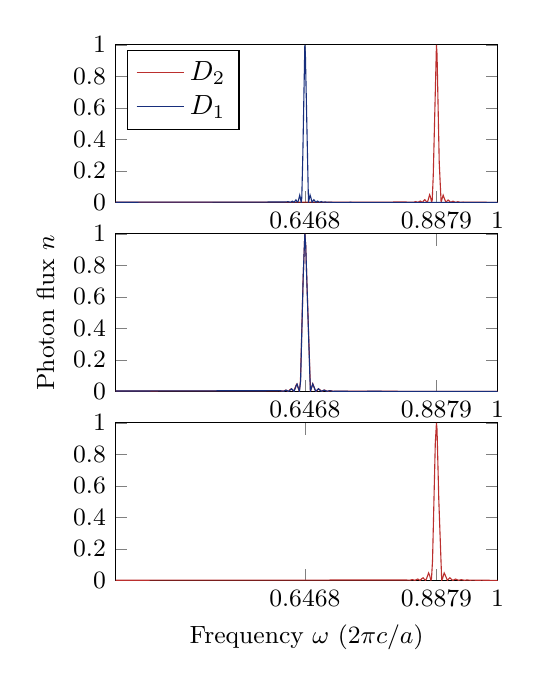
\begin{tikzpicture}

\begin{axis}[%
width=0.4\figW,
height=0.5\figH,
at={(0\figW,1.2\figH)},
scale only axis,
xmin=0.3,
xmax=1,
xtick={0,0.6468,0.8879,1},
xticklabels={$0$,$0.6468$, $0.8879$,$1$},
ymin=0,
ymax=1,
axis background/.style={fill=white},
legend pos = north west
]
\addplot [color=mode2]
  table[row sep=crcr]{%
0	1.13081867070264e-06\\
0.831674911128847	0.00228169467746064\\
0.838881336867126	0.00202377499498518\\
0.842618002064753	0.0021823789198463\\
0.845820857948432	0.000498850577067556\\
0.849824427803032	0.00520157028131374\\
0.853827997657632	0.000158448678008183\\
0.858365376826178	0.00870591815290878\\
0.862102042023805	5.71739905264046e-05\\
0.865304897907484	0.0133645158166602\\
0.866639421192351	0.0173069295692947\\
0.869041563105111	0.00685264541172503\\
0.870642991046951	5.45500426432088e-05\\
0.872244418988791	0.00968327963340587\\
0.87544727487247	0.048612317596354\\
0.87704870281431	0.0344557748770749\\
0.879183940070097	0.000143863495585039\\
0.88025155869799	0.0162957894625595\\
0.882119891296803	0.170638303761119\\
0.887991793750216	1\\
0.889059412378109	0.94000608315541\\
0.893062982232709	0.255338855812756\\
0.896532742773362	4.8698814648418e-05\\
0.898134170715202	0.0209729769593403\\
0.900269407970989	0.0458723635961076\\
0.902404645226775	0.0252393913145816\\
0.905340596453482	9.65076844801072e-05\\
0.909344166308081	0.0156763040359307\\
0.914148450133601	0.000139489728146369\\
0.918152019988201	0.00780486864007757\\
0.92295630381372	0.000160502704093402\\
0.927226778325293	0.00448871207940704\\
0.932031062150813	0.00033301513591999\\
0.936835345976332	0.00232446948495424\\
0.941639629801852	0.000858887074389303\\
0.946177008970398	0.00117400414562741\\
0.950981292795918	0.00101797533071468\\
0.962458193045771	0.00106641777035499\\
0.969397714127077	0.000883365111032708\\
1.00196008227782	0.000118551983291804\\
1.02357935949266	0.000217825320773857\\
1.05854386955616	0.000104712082806824\\
1.15596406935142	4.98964502413379e-05\\
1.3342563802096	7.9476366254827e-06\\
};
\addlegendentry{$D_2$};
\addplot [color=mode1]
  table[row sep=crcr]{%
0	1.39644351637713e-08\\
0.609076427213103	0.00233545672979218\\
0.616282852951382	0.00430043014561177\\
0.620553327462955	0.000248637961077769\\
0.623756183346635	0.00794154826945515\\
0.626959039230315	7.47971153032267e-05\\
0.630428799770968	0.0162317707623461\\
0.632830941683728	0.00204526366888014\\
0.634699274282541	0.00886138610265252\\
0.637368320852274	0.0457755204955326\\
0.638969748794114	0.0193771513115848\\
0.640037367422007	0.000188198916072357\\
0.641104986049901	0.0271105460388243\\
0.642973318648714	0.289533327408285\\
0.64670998384634	1\\
0.647777602474233	0.934370010222459\\
0.653382600270673	0.00025932622168523\\
0.654717123555539	0.0216863788474451\\
0.656318551497379	0.0470796939868294\\
0.657653074782246	0.0325194712216197\\
0.660055216695006	3.53592225057486e-05\\
0.663258072578686	0.0169734429174946\\
0.666994737776312	8.14290493287295e-05\\
0.669930689003018	0.00862561475450141\\
0.673667354200645	4.6983461483352e-05\\
0.676870210084324	0.00514223972653949\\
0.680606875281951	0.000200359717916987\\
0.683809731165631	0.00342867981165518\\
0.687546396363257	0.000316680510486389\\
0.69101615690391	0.00206216482641941\\
0.69501972675851	0.000905361107496283\\
0.699557105927056	0.000132641242323706\\
0.706496627008362	3.5452938580427e-05\\
0.713436148089669	9.90346817442145e-07\\
0.720642573827948	4.63588478374355e-05\\
0.730251141478987	0.000719353650030063\\
0.741461137071867	0.000186432024472216\\
0.758276130461185	0.000260226636216387\\
0.782297549588784	0.00020597772171671\\
1.3342563802096	1.2617425668715e-06\\
};
\addlegendentry{$D_1$};
\end{axis}

\begin{axis}[%
width=0.4\figW,
height=0.5\figH,
at={(0\figW,0.6\figH)},
scale only axis,
xmin=0.3,
xmax=1,
xtick={0,0.6468,0.8879,1},
xticklabels={$0$,$0.6468$, $0.8879$,$1$},
ymin=0,
ymax=1,
axis background/.style={fill=white},
ylabel={Photon flux $n$}
]
\addplot [color=mode2]
table[row sep=crcr]{%
	0	2.23814667652533e-05\\
	0.599467859562064	0.00433628591280777\\
	0.607208094614289	0.00142683721257098\\
	0.611478569125863	0.00804573548853171\\
	0.616015948294409	2.38495126281268e-05\\
	0.621620946090848	0.0165221829549806\\
	0.626425229916368	0.000103599094986251\\
	0.630695704427941	0.0391146642895677\\
	0.632030227712808	0.0463381738836528\\
	0.634966178939514	0.0150116981517305\\
	0.636567606881354	0.000103582077880748\\
	0.638702844137141	0.0650888340040292\\
	0.64350712796266	0.709716332149051\\
	0.64670998384634	1\\
	0.64831141178818	0.928598166077518\\
	0.657119265468299	5.24822337082398e-05\\
	0.661389739979872	0.0480230679381304\\
	0.665660214491445	0.00758763999999168\\
	0.667528547090259	6.15704802147121e-05\\
	0.672065926258805	0.0163909949062666\\
	0.677937828712218	0.000108656655533057\\
	0.682742112537738	0.00847027912289966\\
	0.688347110334177	9.69307907228156e-05\\
	0.693685203473643	0.00469925536614135\\
	0.699290201270083	0.000427018840210458\\
	0.706763531665336	0.000799353937359193\\
	0.73692375790332	0.000616286557307388\\
	1.04172887616684	6.40938787921375e-05\\
	1.3342563802096	8.46451827918315e-06\\
};
\addplot [color=mode1]
table[row sep=crcr]{%
	0	1.56938971469511e-05\\
	0.601069287503903	0.00451669176492464\\
	0.60800880858521	0.000851375047454139\\
	0.612279283096783	0.00805966375870093\\
	0.617083566922302	9.43746109351995e-05\\
	0.622421660061768	0.0163816251332891\\
	0.626959039230315	4.73278638151164e-05\\
	0.630962609084915	0.0368452763636986\\
	0.632564037026754	0.0462407726858916\\
	0.636834511538327	2.87090439536897e-05\\
	0.638969748794114	0.0661715327694608\\
	0.643774032619634	0.733609777486815\\
	0.64670998384634	1\\
	0.64831141178818	0.926810610112689\\
	0.656852360811326	8.02636681402902e-05\\
	0.661122835322899	0.0475272659011989\\
	0.666727833119339	8.47098536960189e-06\\
	0.671532116944858	0.0167160835620319\\
	0.676870210084324	1.7232287029989e-05\\
	0.681674493909844	0.008387982526882\\
	0.687279491706284	0.000175526652539837\\
	0.692350680188777	0.0048707240118413\\
	0.697688773328243	0.000322623719081649\\
	0.704895199066522	0.000921248344013526\\
	0.73532232996148	0.000254606514388689\\
	0.772955886594717	0.000574892630722301\\
	0.819664201565048	0.000238753269072856\\
	1.06735172323628	5.2218821191552e-06\\
	1.3342563802096	1.2676653494248e-05\\
};
\end{axis}


\begin{axis}[%
width=0.4\figW,
height=0.5\figH,
at={(0\figW,0\figH)},
scale only axis,
xlabel = {Frequency $\omega$ ($2 \pi c/a$)},
xmin=0.3,
xmax=1,
xtick={0,0.6468,0.8879,1},
xticklabels={$0$,$0.6468$, $0.8879$,$1$},
ymin=0,
ymax=1,
axis background/.style={fill=white}
]
\addplot [color=mode2]
table[row sep=crcr]{%
	0	1.22034047884689e-05\\
	0.8311411018149	0.0023013266385894\\
	0.835411576326473	0.00175360932962421\\
	0.839415146181073	0.000965341281125021\\
	0.843685620692646	0.00486553930555145\\
	0.848489904518166	0.000250045011197297\\
	0.853561093000659	0.00825574609007673\\
	0.858098472169205	4.97169960933519e-05\\
	0.861301328052885	0.0109829985996603\\
	0.863436565308671	0.0163494616861442\\
	0.866372516535378	0.00457764465273192\\
	0.867973944477217	1.94703586926526e-05\\
	0.870109181733004	0.013154486929305\\
	0.873578942273657	0.0470453003425026\\
	0.87544727487247	0.0315310399247428\\
	0.87784941678523	2.28975304077395e-05\\
	0.878917035413123	0.0124357545233098\\
	0.880785368011937	0.12400183153239\\
	0.885856556494429	0.869270322219562\\
	0.887991793750216	1\\
	0.889059412378109	0.957556042194106\\
	0.892262268261789	0.513878092808121\\
	0.897600361401255	0.00108842262365672\\
	0.899201789343095	0.0122024441442494\\
	0.902137740569802	0.047153720606177\\
	0.904272977825588	0.0315377211631087\\
	0.908009643023215	1.99441444377335e-05\\
	0.912547022191761	0.0164419581043247\\
	0.916016782732414	0.0041292680012357\\
	0.918152019988201	5.37346492168744e-05\\
	0.92295630381372	0.00824687137239732\\
	0.92856130161016	0.000227034194552944\\
	0.933632490092653	0.00460027207861069\\
	0.938970583232119	0.000392405550539987\\
	0.944308676371585	0.00264766067464928\\
	0.949646769511052	0.000683950981152037\\
	0.954717957993545	0.00165690344143354\\
	0.960056051133011	0.000724562177670807\\
	0.965394144272477	0.000892302126201283\\
	0.97126604672589	0.0010733450416256\\
	0.986212707516396	0.000294720956906636\\
	1.00943341267307	0.000131287278812842\\
	1.02411316880661	0.00048471950436868\\
	1.04066125753895	0.000233818595714919\\
	1.06841934186418	6.61720048844572e-06\\
	1.10391766124163	0.000200101820605481\\
	1.14662240635736	3.20710461947371e-05\\
	1.3342563802096	4.61615482860722e-05\\
};
\end{axis}
\end{tikzpicture}%
	\end{subfigure}
	\caption[]{Phase matched non-reciprocity in a modulated structure. Note that the slight bending at the edges of the simulation are due to the \textit{PML} layer, and do not affect the final solution.}
	\label{fig:bandyu}
\end{figure} 


\begin{figure}[t]
	\centering
	\setlength{\figH}{0.3\textwidth}
	\setlength{\figW}{0.8\textwidth}
	% This file was created by matlab2tikz.
%
%The latest updates can be retrieved from
%  http://www.mathworks.com/matlabcentral/fileexchange/22022-matlab2tikz-matlab2tikz
%where you can also make suggestions and rate matlab2tikz.
%
\definecolor{mycolor1}{rgb}{0.00000,0.44700,0.74100}%
\definecolor{mycolor2}{rgb}{0.85000,0.32500,0.09800}%
\definecolor{mycolor3}{rgb}{0.92900,0.69400,0.12500}%
\definecolor{mycolor4}{rgb}{0.49400,0.18400,0.55600}%
%
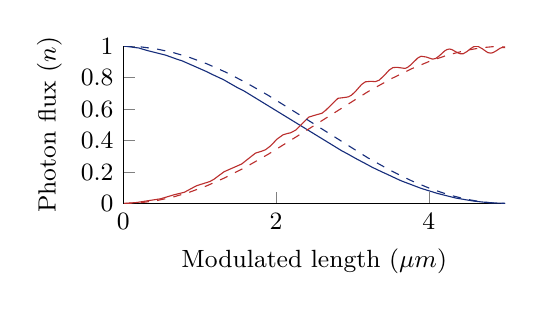
\begin{tikzpicture}

\begin{axis}[%
width=0.4\figW,
height=0.5\figH,
at={(0\figW,0\figH)},
scale only axis,
xmin=0,
xmax=5,
ymin=0,
ymax=1,
xlabel = {Modulated length ($\mu m$)},
ylabel = {Photon flux ($n$)},
axis background/.style={fill=white},
axis x line*=bottom,
axis y line*=left
]
\addplot [color=mode1]
  table[row sep=crcr]{%
0.00999999999999979	1\\
0.13	0.992\\
0.2	0.988\\
0.29	0.975\\
0.35	0.967\\
0.55	0.943\\
0.7	0.917\\
0.77	0.906\\
1.08	0.84\\
1.15	0.823\\
1.31	0.787\\
1.49	0.737\\
1.58	0.715\\
2.86	0.335\\
2.93	0.317\\
3.07	0.279\\
3.15	0.259\\
3.26	0.23\\
3.39	0.2\\
3.44	0.189\\
3.59	0.155\\
3.64	0.144\\
3.9	0.0961999999999996\\
4.11	0.0646000000000004\\
4.35	0.0351999999999997\\
4.59	0.0152999999999999\\
4.8	0.00460999999999956\\
5.01	0.00107000000000035\\
};
\addplot [color=mode2]
  table[row sep=crcr]{%
0.00999999999999979	0.00076699999999974\\
0.17	0.00628000000000029\\
0.49	0.0303000000000004\\
0.66	0.0549999999999997\\
0.8	0.0716000000000001\\
0.9	0.0978000000000003\\
0.96	0.113\\
1.05	0.127\\
1.13	0.139\\
1.19	0.155\\
1.25	0.177\\
1.32	0.202\\
1.55	0.251\\
1.73	0.32\\
1.81	0.332\\
1.86	0.341\\
1.92	0.363\\
1.96	0.382\\
2.01	0.408\\
2.09	0.436\\
2.15	0.445\\
2.19	0.449\\
2.26	0.467\\
2.31	0.491\\
2.43	0.549\\
2.51	0.561\\
2.6	0.573\\
2.65	0.592\\
2.81	0.668\\
2.92	0.675\\
2.95	0.678\\
2.99	0.689\\
3.04	0.712\\
3.12	0.756\\
3.17	0.773\\
3.24	0.776\\
3.3	0.774\\
3.35	0.783\\
3.42	0.815\\
3.48	0.847\\
3.53	0.863\\
3.58	0.865\\
3.69	0.858\\
3.72	0.864\\
3.76	0.879\\
3.86	0.926\\
3.9	0.935000000000001\\
3.96	0.931\\
4.05	0.917\\
4.09	0.921\\
4.14	0.939\\
4.21	0.97\\
4.24	0.978\\
4.27	0.981\\
4.3	0.978\\
4.36	0.962\\
4.41	0.951\\
4.45	0.951\\
4.5	0.965\\
4.54	0.981\\
4.59	0.997\\
4.64	0.999\\
4.7	0.983\\
4.77	0.959\\
4.81	0.955\\
4.84	0.958\\
4.88	0.969\\
4.93	0.985\\
4.96	0.991\\
4.99	0.991\\
5.01	0.988\\
};
\addplot [color=mode1, dashed]
  table[row sep=crcr]{%
0.00999999999999979	0.999990209\\
0.22	0.99526858\\
0.43	0.982005207\\
0.64	0.96042884\\
0.86	0.929316078\\
1.09	0.888113089\\
1.33	0.836575682\\
1.6	0.769602103\\
1.9	0.686271286\\
2.29	0.568622403\\
3.2	0.290741175\\
3.51	0.207120884\\
3.78	0.143143349\\
4.02	0.094757081\\
4.25	0.0569368749999999\\
4.47	0.0293268749999998\\
4.68	0.0112758949999998\\
4.89	0.00165378700000041\\
5.01	9.7910900000997e-06\\
};
\addplot [color=mode2, dashed]
  table[row sep=crcr]{%
0.00999999999999979	9.7910900000997e-06\\
0.22	0.00473141999999971\\
0.43	0.0179947929999997\\
0.64	0.0395711600000004\\
0.86	0.0706839219999997\\
1.09	0.111886911\\
1.33	0.163424318\\
1.6	0.230397897\\
1.9	0.313728714\\
2.29	0.431377597\\
3.2	0.709258825\\
3.51	0.792879116\\
3.78	0.856856651\\
4.02	0.905242919\\
4.25	0.943063125\\
4.47	0.970673125\\
4.68	0.988724105\\
4.89	0.998346213\\
5.01	0.999990209\\
};
\end{axis}
\end{tikzpicture}%
	\caption[The modulated waveguide structure]{LR 12.25 and width 1.1}
	\label{fig:coherencelength}
\end{figure} 

\begin{table}[]
	\centering
	\caption[Mode conversions in a phase-matched structure]{Summary of mode conversions in the phase-matched structure}
	\label{my-label}
	\begin{tabular}{|l|l|}
		\hline 
		Direction & Transition \\ \hline
		LR        & $\ket{1} \rightarrow \ket{2}$           \\
		RL        & $\ket{1} \rightarrow \ket{1}$           \\
		TR        & $\ket{2} \rightarrow \ket{2}$          \\ \hline
	\end{tabular}
\end{table}

\section{Motivation for development of frequency domain solutions}
	
Simulating effective modulations of wave-guide structures is evidently a computationally intensive process. Consider the simplest example, a slab waveguide whose permittivity modulation frequency is tuned to stimulate a photonic transition between the first fundamental () and the second odd mode. This requires the modulation frequency to be (), several orders of magnitude lower than the input wave. Since a time-domain simulation requires the time-step to be chosen based on the highest frequency present in the simulation, the massive gap between the optical source frequency and the modulation frequency lead to slow convergence times. This is because the input wave must pass through at minimum one cycle of the modulation. There are however, several benefits granted by the harmonic nature of the modulation. The first is that the modulation generates sidebands at \textit{known} frequencies,
\begin{equation}
\omega_n = \omega_0 \pm n \Omega
\end{equation}
where $\Omega$ is the modulation frequency and $n$ is the set of integers. This is incredibly advantageous: we know in advance every possible frequency that can exist in the simulation space. The second benefit granted is that the modulation is harmonic in nature, and it is this harmonicity that allows for a method of expressing the time dependent modulations in frequency space. Thus, we look towards a modified form of the finite-difference frequency domain where instead of discretising \textit{time} we discretise \textit{frequency} instead.


\begin{table}[]
\centering
\begin{tabular}{|l|l|l|}
\hline
                             & \textit{Time domain}    & \textit{Frequency domain}         \\ \hline
\textit{Memory usage}        & Medium                  & High                              \\ \hline
\textit{Adjacent eigenmodes} & Mixed in final solution & Naturally separated               \\ \hline
\textit{Standard run-time}   & Days                    & Hours                             \\ \hline
\textit{Parallelisation}   & Trivial                 & Non-trivial \\ \hline
\textit{Extension to 3D}   & Trivial                 & Trivial \\ \hline
\end{tabular}
\caption[Comparison of \textit{FDTD} and \textit{FDFD} methods]{Comparison of basic extraction methods and computational expenditure for general finite difference simulations in the time and frequency domain. In this case, parallelisation refers to the property of being able to split the simulation into multiple `chunks' that can be run simultaneously on high-performance clusters.}
\label{comparisonFD}
\end{table}

In table \ref{comparisonFD} the main properties of the time and frequency domain methods are compared.



    %\chapter{Finite difference frequency domain}

The finite difference frequency domain method is a complementary numerical method of solving Maxwell's equations as an alternative to time domain simulations. 

There are alternatives, however, to obtaining full-wave solutions to Maxwell's equations. Namely, by a suitable transformation into the frequency domain, the problem of time-step based simulations instead becomes one of solving a large system of linear equations in the form

\begin{equation}
Ax = b
\end{equation}

where $A$ is the \textit{wave matrix}, $x$ is a vector that contains information on the electromagnetic fields, and $b$ is a source. Fortuitously, in two dimensions the most efficient method of solving for the field distributions is through the elementary matrix inversion,

\begin{equation}
x = A^{-1}b,
\end{equation}
 
which has the trivial solution of $x=0$ for a zero source simulation ($b=0$). In solving for $x$, one obtains the steady-state solution directly embedded in the matrix, however the frequency domain formulation can only handle one frequency at a time.


\section{The multi-frequency method (MF-FDFD)}
Here, we adapt the frequency domain method to multiple simultaneous frequencies.
Consider the frequency domain Maxwell equations;

\begin{equation}
\nabla \times \mu(\omega)^{-1} - \omega^2 \epsilon_s (\omega) \bm{E}(\omega) - \omega^2 \bm{P}(\omega) = -i \omega \bm{J}(\omega)
\end{equation}

where $\bm{E}(\omega)$ is the electric field distribution at frequency $\omega$, and $\mu(\omega)$ and $\epsilon_s(\omega)$ are the frequency dependent permeability and permittivity respectively. 

Now, we assume a region of the simulation space is altered by the standard permittivity modulation of the form

\begin{equation}
\epsilon(t) = \epsilon_s + \delta cos(\omega t + \phi).
\end{equation}

We can account for this modulation in frequency space by considering its effects on the polarisation of the material in question,

\begin{equation}
	 \delta cos(\omega t + \phi) \bm{E}.
\end{equation}

Through Euler's identity we obtain a more suggestible form

\begin{equation}
\bm{P}(\omega) = \dfrac{\delta}{2} (e^{i(\Omega t + \phi)} + e^{-i(\Omega t + \phi)}) \bm{E}(t).
\end{equation}

Using the standard inverse Fourier transform \footnote{Note that here we are using the inverse Fourier transform to move from the time to the frequency domain, although the forward Fourier transform is just as applicable, and only results in a shifted phase.},

The generation of sidebands by the modulation ensures that the time-domain electric field $\bm{E}(t)$ is the superposition of electric field components at each sideband $n$ (through the linearity of Maxwell's equations),

\begin{equation}
\tilde{\bm{E}}(t) = \Re \{\sum_n \bm{E}(\omega_n)e^{i \omega_n t}\}
\end{equation}


We implement the finite difference method to solve the above equations.

To test the validity of the simulation, we first consider a weakly modulated waveguide ($\delta = 0.001$).  A weak modulation is chosen as it can be readily approximated through coupled mode theory, providing a comparison.

To test the suitability of FDFD, we perform a frequency domain simulation of a dynamically modulated waveguide structure over several side-bands. The waveguide is identical to that of the one simulated via time-domain methods (fig X), with $\epsilon_s = 12.25$, which supports a transverse electric $\text{TE}_{00}$ mode at $w_0 = 0.129 (\frac{2\pi c}{a})$ and a  $\text{TE}_{01}$ mode at $w_1 = 0.198(\frac{2\pi c}{a})$ (see fig Y for bandstructure). For each frequency sideband, we extract the field profile amplitude and compare to the analytical results provided by coupled-mode theory. An eigenmode source is calculated a priori (see appendix Z) much like the time-domain simulations, so that the field profile can be coupled exactly into the waveguide structure. We test both the left-to-right $LR$ and right-to-left $RL$ propagation directions to ensure that parity-symmetry is broken (as is predicted by theory), and set the normalised amplitude to 1UNITS. To test time-reversal symmetry, we inject a $\text{TE}_{01}$ mode from the right-to-left direction.

%\begin{figure}[t]
%	\centering
%	\setlength{\figH}{0.5\textwidth}
%	\setlength{\figW}{1\textwidth}
%	\begin{subfigure}[t]{0.5\textwidth}
%		% This file was created by matlab2tikz.
%
%The latest updates can be retrieved from
%  http://www.mathworks.com/matlabcentral/fileexchange/22022-matlab2tikz-matlab2tikz
%where you can also make suggestions and rate matlab2tikz.
%
\definecolor{mycolor1}{rgb}{0.00000,0.44700,0.74100}%
%
\begin{tikzpicture}

\begin{axis}[%
width=0.75\figW,
height=\figH,
at={(0\figW,0\figH)},
scale only axis,
xmin=0,
xmax=30001,
xlabel style={font=\color{white!15!black}},
xlabel={nz = 155280},
y dir=reverse,
ymin=0,
ymax=30001,
axis background/.style={fill=white}
]
\addplot [color=mycolor1, draw=none, mark size=0.7pt, mark=*, mark options={solid, mycolor1}, forget plot]
  table[row sep=crcr]{%
1	1\\
1	100\\
1	9901\\
72	172\\
78	77\\
78	9978\\
181	281\\
203	103\\
209	309\\
335	235\\
335	334\\
335	435\\
483	583\\
489	389\\
541	641\\
592	492\\
592	692\\
689	789\\
720	721\\
746	846\\
849	749\\
849	848\\
849	949\\
1003	903\\
1003	1002\\
1032	1132\\
1101	1201\\
1106	1006\\
1209	1309\\
1232	1132\\
1238	1338\\
1363	1263\\
1363	1362\\
1363	1463\\
1512	1612\\
1518	1418\\
1569	1669\\
1621	1521\\
1621	1721\\
1718	1818\\
1748	1749\\
1775	1875\\
1878	1778\\
1878	1877\\
1878	1978\\
2032	1932\\
2032	2031\\
2061	2161\\
2129	2229\\
2135	2035\\
2238	2338\\
2261	2161\\
2266	2366\\
2392	2292\\
2392	2391\\
2392	2492\\
2541	2641\\
2546	2446\\
2598	2698\\
2649	2549\\
2649	2749\\
2746	2846\\
2777	2778\\
2803	2903\\
2906	2806\\
2906	2905\\
2906	3006\\
3061	2961\\
3061	3060\\
3089	3189\\
3158	3258\\
3163	3063\\
3266	3366\\
3289	3189\\
3295	3395\\
3421	3321\\
3421	3420\\
3421	3521\\
3569	3669\\
3575	3475\\
3626	3726\\
3678	3578\\
3678	3778\\
3775	3875\\
3805	3806\\
3832	3932\\
3935	3835\\
3935	3934\\
3935	4035\\
3941	13941\\
3986	13986\\
4089	3989\\
4089	4088\\
4089	14089\\
4118	4218\\
4161	14161\\
4186	4286\\
4192	4092\\
4192	14192\\
4295	4395\\
4318	4218\\
4324	4424\\
4346	14346\\
4441	14441\\
4449	4349\\
4449	4448\\
4449	4549\\
4541	14541\\
4572	14572\\
4598	4698\\
4604	4504\\
4655	4755\\
4706	4606\\
4706	4806\\
4741	14741\\
4804	4904\\
4834	4835\\
4841	14841\\
4861	4961\\
4964	4864\\
4964	4963\\
4964	5064\\
4964	14964\\
5041	15041\\
5118	5018\\
5118	5117\\
5141	15141\\
5146	5246\\
5190	15190\\
5215	5315\\
5221	5121\\
5241	15241\\
5324	5424\\
5341	15341\\
5346	5246\\
5352	5452\\
5375	15375\\
5478	5378\\
5478	5477\\
5478	5578\\
5478	15478\\
5541	15541\\
5626	5726\\
5632	5532\\
5641	15641\\
5684	5784\\
5735	5635\\
5735	5835\\
5741	15741\\
5832	5932\\
5863	5864\\
5875	15875\\
5889	5989\\
5992	5892\\
5992	5991\\
5992	6092\\
5992	15992\\
6041	16041\\
6146	6046\\
6146	6145\\
6175	6275\\
6244	6344\\
6249	6149\\
6352	6452\\
6375	6275\\
6381	6481\\
6506	6406\\
6506	6505\\
6506	6606\\
6655	6755\\
6661	6561\\
6712	6812\\
6764	6664\\
6764	6864\\
6861	6961\\
6891	6892\\
6918	7018\\
7021	6921\\
7021	7020\\
7021	7121\\
7175	7075\\
7175	7174\\
7204	7304\\
7272	7372\\
7278	7178\\
7381	7481\\
7404	7304\\
7409	7509\\
7535	7435\\
7535	7534\\
7535	7635\\
7684	7784\\
7689	7589\\
7741	7841\\
7792	7692\\
7792	7892\\
7889	7989\\
7920	7921\\
7946	8046\\
8049	7949\\
8049	8048\\
8049	8149\\
8204	8104\\
8204	8203\\
8232	8332\\
8301	8401\\
8306	8206\\
8409	8509\\
8432	8332\\
8438	8538\\
8564	8464\\
8564	8563\\
8564	8664\\
8712	8812\\
8718	8618\\
8769	8869\\
8821	8721\\
8821	8921\\
8918	9018\\
8948	8949\\
8975	9075\\
9078	8978\\
9078	9077\\
9078	9178\\
9232	9132\\
9232	9231\\
9261	9361\\
9329	9429\\
9335	9235\\
9438	9538\\
9461	9361\\
9467	9567\\
9592	9492\\
9592	9591\\
9592	9692\\
9741	9841\\
9747	9647\\
9798	9898\\
9849	9749\\
9849	9949\\
9901	1\\
9977	9978\\
10001	10100\\
10001	19901\\
10090	19990\\
10100	10001\\
10107	10106\\
10107	10207\\
10261	10161\\
10261	10260\\
10289	10389\\
10358	10458\\
10364	10264\\
10467	10567\\
10489	10389\\
10495	10595\\
10621	10521\\
10621	10620\\
10621	10721\\
10769	10869\\
10775	10675\\
10827	10927\\
10878	10778\\
10878	10978\\
10975	11075\\
11006	11007\\
11032	11132\\
11135	11035\\
11135	11134\\
11135	11235\\
11289	11189\\
11289	11288\\
11318	11418\\
11387	11487\\
11392	11292\\
11495	11595\\
11518	11418\\
11524	11624\\
11649	11549\\
11649	11648\\
11649	11749\\
11798	11898\\
11804	11704\\
11855	11955\\
11907	11807\\
11907	12007\\
12004	12104\\
12034	12035\\
12061	12161\\
12164	12064\\
12164	12163\\
12164	12264\\
12318	12218\\
12318	12317\\
12347	12447\\
12415	12515\\
12421	12321\\
12524	12624\\
12547	12447\\
12552	12652\\
12678	12578\\
12678	12677\\
12678	12778\\
12827	12927\\
12832	12732\\
12884	12984\\
12935	12835\\
12935	13035\\
13032	13132\\
13063	13064\\
13090	13190\\
13192	13092\\
13192	13191\\
13192	13292\\
13347	13247\\
13347	13346\\
13375	13475\\
13444	13544\\
13450	13350\\
13552	13652\\
13575	13475\\
13581	13681\\
13707	13607\\
13707	13706\\
13707	13807\\
13855	13955\\
13861	13761\\
13912	14012\\
13941	3941\\
13941	23941\\
13964	3964\\
13964	13864\\
13964	14064\\
13964	23964\\
14041	4041\\
14061	14161\\
14081	4081\\
14091	14092\\
14118	14218\\
14141	24141\\
14221	14121\\
14221	14220\\
14221	14321\\
14241	4241\\
14241	24241\\
14272	24272\\
14341	4341\\
14341	24341\\
14375	4375\\
14375	14275\\
14375	14374\\
14404	14504\\
14441	24441\\
14472	14572\\
14478	4478\\
14478	14378\\
14478	24478\\
14561	4561\\
14581	14681\\
14604	14504\\
14610	14710\\
14641	4641\\
14641	24641\\
14735	14635\\
14735	14734\\
14735	14835\\
14741	4741\\
14741	24741\\
14787	24787\\
14858	24858\\
14884	14984\\
14890	4890\\
14890	14790\\
14941	15041\\
14992	4992\\
14992	14892\\
14992	15092\\
14992	24992\\
15090	15190\\
15095	5095\\
15120	15121\\
15141	5141\\
15141	25141\\
15147	15247\\
15241	25241\\
15246	5246\\
15250	15150\\
15250	15249\\
15250	15350\\
15341	25341\\
15384	5384\\
15404	15304\\
15404	15403\\
15432	15532\\
15441	5441\\
15441	25441\\
15476	25476\\
15501	15601\\
15507	15407\\
15541	5541\\
15541	25541\\
15589	5589\\
15610	15710\\
15632	15532\\
15638	15738\\
15641	5641\\
15641	25641\\
15764	5764\\
15764	15664\\
15764	15763\\
15764	15864\\
15764	25764\\
15841	25841\\
15887	25887\\
15912	16012\\
15918	15818\\
15941	5941\\
15970	16070\\
16021	15921\\
16021	16121\\
16041	6041\\
16041	26041\\
16118	16218\\
16149	16150\\
16175	16275\\
16278	16178\\
16278	16277\\
16278	16378\\
16432	16332\\
16432	16431\\
16461	16561\\
16530	16630\\
16535	16435\\
16638	16738\\
16661	16561\\
16667	16767\\
16792	16692\\
16792	16791\\
16792	16892\\
16941	17041\\
16947	16847\\
16998	17098\\
17050	16950\\
17050	17150\\
17147	17247\\
17177	17178\\
17204	17304\\
17307	17207\\
17307	17306\\
17307	17407\\
17461	17361\\
17461	17460\\
17490	17590\\
17558	17658\\
17564	17464\\
17667	17767\\
17690	17590\\
17695	17795\\
17821	17721\\
17821	17820\\
17821	17921\\
17970	18070\\
17975	17875\\
18027	18127\\
18078	17978\\
18078	18178\\
18175	18275\\
18206	18207\\
18233	18333\\
18335	18235\\
18335	18334\\
18335	18435\\
18490	18390\\
18490	18489\\
18518	18618\\
18587	18687\\
18593	18493\\
18695	18795\\
18718	18618\\
18724	18824\\
18850	18750\\
18850	18849\\
18850	18950\\
18998	19098\\
19004	18904\\
19055	19155\\
19107	19007\\
19107	19207\\
19204	19304\\
19234	19235\\
19261	19361\\
19364	19264\\
19364	19363\\
19364	19464\\
19518	19418\\
19518	19517\\
19547	19647\\
19615	19715\\
19621	19521\\
19724	19824\\
19747	19647\\
19753	19853\\
19878	19778\\
19878	19877\\
19878	19978\\
19901	10001\\
19930	10030\\
20001	20100\\
20001	29901\\
20033	29933\\
20084	20184\\
20135	20035\\
20135	20235\\
20233	20333\\
20263	20264\\
20290	20390\\
20393	20293\\
20393	20392\\
20393	20493\\
20547	20447\\
20547	20546\\
20575	20675\\
20644	20744\\
20650	20550\\
20753	20853\\
20775	20675\\
20781	20881\\
20907	20807\\
20907	20906\\
20907	21007\\
21055	21155\\
21061	20961\\
21113	21213\\
21164	21064\\
21164	21264\\
21261	21361\\
21292	21293\\
21318	21418\\
21421	21321\\
21421	21420\\
21421	21521\\
21576	21476\\
21576	21575\\
21604	21704\\
21673	21773\\
21678	21578\\
21781	21881\\
21804	21704\\
21810	21910\\
21936	21836\\
21936	21935\\
21936	22036\\
22084	22184\\
22090	21990\\
22141	22241\\
22193	22093\\
22193	22293\\
22290	22390\\
22320	22321\\
22347	22447\\
22450	22350\\
22450	22449\\
22450	22550\\
22604	22504\\
22604	22603\\
22633	22733\\
22701	22801\\
22707	22607\\
22810	22910\\
22833	22733\\
22838	22938\\
22964	22864\\
22964	22963\\
22964	23064\\
23113	23213\\
23118	23018\\
23170	23270\\
23221	23121\\
23221	23321\\
23318	23418\\
23349	23350\\
23376	23476\\
23478	23378\\
23478	23477\\
23478	23578\\
23633	23533\\
23633	23632\\
23661	23761\\
23730	23830\\
23736	23636\\
23838	23938\\
23861	23761\\
23867	23967\\
23941	13941\\
23993	13993\\
23993	23893\\
23993	23992\\
23993	24093\\
24141	24241\\
24147	14147\\
24147	24047\\
24198	24298\\
24241	14241\\
24250	24150\\
24250	24350\\
24341	14341\\
24347	24447\\
24367	14367\\
24377	24378\\
24404	24504\\
24507	24407\\
24507	24506\\
24507	24607\\
24541	14541\\
24641	14641\\
24661	14661\\
24661	24561\\
24661	24660\\
24690	24790\\
24758	24858\\
24764	14764\\
24764	24664\\
24841	14841\\
24867	24967\\
24890	24790\\
24896	24996\\
24941	14941\\
25021	24921\\
25021	25020\\
25021	25121\\
25041	15041\\
25141	15141\\
25170	25270\\
25176	15176\\
25176	25076\\
25227	25327\\
25278	15278\\
25278	25178\\
25278	25378\\
25376	25476\\
25381	15381\\
25395	15395\\
25406	25407\\
25433	25533\\
25536	25436\\
25536	25535\\
25536	25636\\
25541	15541\\
25670	15670\\
25690	15690\\
25690	25590\\
25690	25689\\
25719	25819\\
25787	25887\\
25793	15793\\
25793	25693\\
25875	15875\\
25896	25996\\
25919	25819\\
25924	26024\\
25944	15944\\
26041	16041\\
26050	25950\\
26050	26049\\
26050	26150\\
26199	26299\\
26204	26104\\
26256	26356\\
26307	26207\\
26307	26407\\
26404	26504\\
26435	26436\\
26461	26561\\
26564	26464\\
26564	26563\\
26564	26664\\
26719	26619\\
26719	26718\\
26747	26847\\
26816	26916\\
26821	26721\\
26924	27024\\
26947	26847\\
26953	27053\\
27079	26979\\
27079	27078\\
27079	27179\\
27227	27327\\
27233	27133\\
27284	27384\\
27336	27236\\
27336	27436\\
27433	27533\\
27463	27464\\
27490	27590\\
27593	27493\\
27593	27592\\
27593	27693\\
27747	27647\\
27747	27746\\
27776	27876\\
27844	27944\\
27850	27750\\
27953	28053\\
27976	27876\\
27981	28081\\
28107	28007\\
28107	28106\\
28107	28207\\
28256	28356\\
28261	28161\\
28313	28413\\
28364	28264\\
28364	28464\\
28461	28561\\
28492	28493\\
28519	28619\\
28621	28521\\
28621	28620\\
28621	28721\\
28776	28676\\
28776	28775\\
28804	28904\\
28873	28973\\
28879	28779\\
28981	29081\\
29004	28904\\
29010	29110\\
29136	29036\\
29136	29135\\
29136	29236\\
29284	29384\\
29290	29190\\
29341	29441\\
29393	29293\\
29393	29493\\
29490	29590\\
29520	29521\\
29547	29647\\
29650	29550\\
29650	29649\\
29650	29750\\
29804	29704\\
29804	29803\\
29833	29933\\
29901	20001\\
29907	29807\\
29932	29933\\
30000	30000\\
};
\end{axis}
\end{tikzpicture}%
%	\end{subfigure}%
%	\begin{subfigure}[t]{0.5\textwidth}
%		% This file was created by matlab2tikz.
%
%The latest updates can be retrieved from
%  http://www.mathworks.com/matlabcentral/fileexchange/22022-matlab2tikz-matlab2tikz
%where you can also make suggestions and rate matlab2tikz.
%
\definecolor{mycolor1}{rgb}{0.00000,0.44700,0.74100}%
%
\begin{tikzpicture}

\begin{axis}[%
width=0.75\figW,
height=\figH,
at={(0\figW,0\figH)},
scale only axis,
xmin=0,
xmax=10001,
xlabel style={font=\color{white!15!black}},
xlabel={nz = 50000},
y dir=reverse,
ymin=0,
ymax=10001,
axis background/.style={fill=white}
]
\addplot [color=mycolor1, draw=none, mark size=0.7pt, mark=*, mark options={solid, mycolor1}, forget plot]
  table[row sep=crcr]{%
1	1\\
1	100\\
1	9901\\
26	25\\
26	126\\
26	9926\\
34	35\\
43	143\\
72	172\\
78	77\\
78	9978\\
95	94\\
100	1\\
112	12\\
112	111\\
112	212\\
129	29\\
146	145\\
158	58\\
163	162\\
163	263\\
194	195\\
198	98\\
198	298\\
215	214\\
215	315\\
240	241\\
249	149\\
249	349\\
262	263\\
278	378\\
283	183\\
283	282\\
283	383\\
301	201\\
318	317\\
323	423\\
331	332\\
335	235\\
335	435\\
363	263\\
369	269\\
369	368\\
369	469\\
377	378\\
386	486\\
409	309\\
415	515\\
421	321\\
421	420\\
438	437\\
455	355\\
455	454\\
455	555\\
472	372\\
489	488\\
500	401\\
506	505\\
506	606\\
537	538\\
541	441\\
541	641\\
558	557\\
558	658\\
582	583\\
592	492\\
592	692\\
605	606\\
621	721\\
626	526\\
626	625\\
626	726\\
643	543\\
661	660\\
666	766\\
674	675\\
678	578\\
678	778\\
706	606\\
712	612\\
712	711\\
712	812\\
720	721\\
729	829\\
752	652\\
758	858\\
763	663\\
763	762\\
781	780\\
798	698\\
798	797\\
798	898\\
815	715\\
832	831\\
843	743\\
849	848\\
849	949\\
880	881\\
883	783\\
883	983\\
901	901\\
918	1018\\
925	926\\
935	835\\
935	1035\\
948	949\\
963	1063\\
969	869\\
969	968\\
969	1069\\
986	886\\
1003	1002\\
1009	1109\\
1017	1018\\
1021	921\\
1021	1121\\
1049	949\\
1055	955\\
1055	1054\\
1055	1155\\
1062	1063\\
1072	1172\\
1095	995\\
1101	1201\\
1106	1006\\
1106	1105\\
1123	1122\\
1141	1041\\
1141	1140\\
1141	1241\\
1158	1058\\
1175	1174\\
1186	1086\\
1192	1191\\
1192	1292\\
1222	1223\\
1226	1126\\
1226	1326\\
1243	1242\\
1243	1343\\
1268	1269\\
1278	1178\\
1278	1378\\
1291	1292\\
1306	1406\\
1312	1212\\
1312	1311\\
1312	1412\\
1329	1229\\
1346	1345\\
1352	1452\\
1360	1361\\
1363	1263\\
1363	1463\\
1392	1292\\
1398	1298\\
1398	1397\\
1398	1498\\
1405	1406\\
1415	1515\\
1438	1338\\
1444	1544\\
1449	1349\\
1449	1448\\
1466	1465\\
1483	1383\\
1484	1483\\
1484	1584\\
1501	1401\\
1518	1517\\
1529	1429\\
1535	1534\\
1535	1635\\
1565	1566\\
1569	1469\\
1569	1669\\
1586	1585\\
1586	1686\\
1611	1612\\
1621	1521\\
1621	1721\\
1634	1635\\
1649	1749\\
1655	1555\\
1655	1654\\
1655	1755\\
1672	1572\\
1689	1688\\
1695	1795\\
1703	1704\\
1706	1606\\
1706	1806\\
1735	1635\\
1741	1641\\
1741	1740\\
1741	1841\\
1748	1749\\
1758	1858\\
1781	1681\\
1786	1886\\
1792	1692\\
1792	1791\\
1809	1808\\
1826	1726\\
1826	1825\\
1826	1926\\
1844	1744\\
1861	1860\\
1872	1772\\
1878	1877\\
1878	1978\\
1908	1909\\
1912	1812\\
1912	2012\\
1929	1928\\
1929	2029\\
1954	1955\\
1964	1864\\
1964	2064\\
1977	1978\\
1992	2092\\
1998	1898\\
1998	1997\\
1998	2098\\
2015	1915\\
2032	2031\\
2038	2138\\
2045	2046\\
2049	1949\\
2049	2149\\
2078	1978\\
2084	1984\\
2084	2083\\
2084	2184\\
2091	2092\\
2106	2206\\
2124	2024\\
2129	2229\\
2135	2035\\
2135	2134\\
2152	2151\\
2169	2069\\
2169	2168\\
2169	2269\\
2186	2086\\
2204	2203\\
2215	2115\\
2221	2220\\
2221	2321\\
2251	2252\\
2255	2155\\
2255	2355\\
2272	2271\\
2272	2372\\
2297	2298\\
2306	2206\\
2306	2406\\
2320	2321\\
2335	2435\\
2341	2241\\
2341	2340\\
2341	2441\\
2358	2258\\
2375	2374\\
2381	2481\\
2388	2389\\
2392	2292\\
2392	2492\\
2421	2321\\
2426	2326\\
2426	2425\\
2426	2526\\
2434	2435\\
2444	2544\\
2466	2366\\
2472	2572\\
2478	2378\\
2478	2477\\
2495	2494\\
2512	2412\\
2512	2511\\
2512	2612\\
2529	2429\\
2546	2545\\
2558	2458\\
2564	2563\\
2564	2664\\
2594	2595\\
2598	2498\\
2598	2698\\
2615	2614\\
2615	2715\\
2640	2641\\
2649	2549\\
2649	2749\\
2663	2664\\
2678	2778\\
2684	2584\\
2684	2683\\
2684	2784\\
2701	2601\\
2718	2717\\
2724	2824\\
2731	2732\\
2735	2635\\
2735	2835\\
2764	2664\\
2769	2669\\
2769	2768\\
2769	2869\\
2777	2778\\
2792	2892\\
2809	2709\\
2815	2915\\
2821	2721\\
2821	2820\\
2838	2837\\
2855	2755\\
2855	2854\\
2855	2955\\
2872	2772\\
2889	2888\\
2900	2801\\
2907	2906\\
2907	3007\\
2937	2938\\
2941	2841\\
2941	3041\\
2958	2957\\
2958	3058\\
2983	2984\\
2992	2892\\
2992	3092\\
3006	3007\\
3021	3121\\
3027	2927\\
3027	3026\\
3027	3127\\
3044	2944\\
3061	3060\\
3067	3167\\
3074	3075\\
3078	2978\\
3078	3178\\
3107	3007\\
3112	3012\\
3112	3111\\
3112	3212\\
3120	3121\\
3129	3229\\
3152	3052\\
3158	3258\\
3164	3064\\
3164	3163\\
3181	3180\\
3198	3098\\
3198	3197\\
3198	3298\\
3215	3115\\
3232	3231\\
3244	3144\\
3249	3248\\
3249	3349\\
3280	3281\\
3284	3184\\
3284	3384\\
3301	3301\\
3318	3418\\
3326	3327\\
3335	3235\\
3335	3435\\
3348	3349\\
3364	3464\\
3369	3269\\
3369	3368\\
3369	3469\\
3387	3287\\
3404	3403\\
3409	3509\\
3417	3418\\
3421	3321\\
3421	3521\\
3449	3349\\
3455	3355\\
3455	3454\\
3455	3555\\
3463	3464\\
3472	3572\\
3495	3395\\
3501	3601\\
3507	3407\\
3507	3506\\
3524	3523\\
3541	3441\\
3541	3540\\
3541	3641\\
3558	3458\\
3575	3574\\
3587	3487\\
3592	3591\\
3592	3692\\
3623	3624\\
3627	3527\\
3627	3727\\
3644	3643\\
3644	3744\\
3668	3669\\
3678	3578\\
3678	3778\\
3691	3692\\
3707	3807\\
3712	3612\\
3712	3711\\
3712	3812\\
3729	3629\\
3747	3746\\
3752	3852\\
3760	3761\\
3764	3664\\
3764	3864\\
3792	3692\\
3798	3698\\
3798	3797\\
3798	3898\\
3806	3807\\
3815	3915\\
3838	3738\\
3844	3944\\
3849	3749\\
3849	3848\\
3867	3866\\
3884	3784\\
3884	3883\\
3884	3984\\
3901	3801\\
3918	3917\\
3929	3829\\
3935	3934\\
3935	4035\\
3966	3967\\
3969	3869\\
3969	4069\\
3987	3986\\
3987	4087\\
4011	4012\\
4021	3921\\
4021	4121\\
4034	4035\\
4049	4149\\
4055	3955\\
4055	4054\\
4055	4155\\
4072	3972\\
4089	4088\\
4095	4195\\
4103	4104\\
4107	4007\\
4107	4207\\
4135	4035\\
4141	4041\\
4141	4140\\
4141	4241\\
4148	4149\\
4158	4258\\
4181	4081\\
4187	4287\\
4192	4092\\
4192	4191\\
4209	4208\\
4227	4127\\
4227	4226\\
4227	4327\\
4244	4144\\
4261	4260\\
4272	4172\\
4278	4277\\
4278	4378\\
4309	4310\\
4312	4212\\
4312	4412\\
4330	4329\\
4330	4430\\
4354	4355\\
4364	4264\\
4364	4464\\
4377	4378\\
4392	4492\\
4398	4298\\
4398	4397\\
4398	4498\\
4415	4315\\
4432	4431\\
4438	4538\\
4446	4447\\
4450	4350\\
4450	4550\\
4478	4378\\
4484	4384\\
4484	4483\\
4484	4584\\
4491	4492\\
4507	4607\\
4524	4424\\
4530	4630\\
4535	4435\\
4535	4534\\
4552	4551\\
4570	4470\\
4570	4569\\
4570	4670\\
4587	4487\\
4604	4603\\
4615	4515\\
4621	4620\\
4621	4721\\
4651	4652\\
4655	4555\\
4655	4755\\
4672	4671\\
4672	4772\\
4697	4698\\
4707	4607\\
4707	4807\\
4720	4721\\
4735	4835\\
4741	4641\\
4741	4740\\
4741	4841\\
4758	4658\\
4775	4774\\
4781	4881\\
4789	4790\\
4792	4692\\
4792	4892\\
4821	4721\\
4827	4727\\
4827	4826\\
4827	4927\\
4834	4835\\
4844	4944\\
4867	4767\\
4872	4972\\
4878	4778\\
4878	4877\\
4895	4894\\
4912	4812\\
4912	4911\\
4912	5012\\
4930	4830\\
4947	4946\\
4958	4858\\
4964	4963\\
4964	5064\\
4994	4995\\
4998	4898\\
4998	5098\\
5015	5014\\
5015	5115\\
5040	5041\\
5050	4950\\
5050	5150\\
5063	5064\\
5078	5178\\
5084	4984\\
5084	5083\\
5084	5184\\
5101	5001\\
5118	5117\\
5124	5224\\
5131	5132\\
5135	5035\\
5135	5235\\
5164	5064\\
5170	5070\\
5170	5169\\
5170	5270\\
5177	5178\\
5187	5287\\
5210	5110\\
5215	5315\\
5221	5121\\
5221	5220\\
5238	5237\\
5255	5155\\
5255	5254\\
5255	5355\\
5272	5172\\
5290	5289\\
5300	5201\\
5307	5306\\
5307	5407\\
5337	5338\\
5341	5241\\
5341	5441\\
5358	5357\\
5358	5458\\
5383	5384\\
5392	5292\\
5392	5492\\
5406	5407\\
5421	5521\\
5427	5327\\
5427	5426\\
5427	5527\\
5444	5344\\
5461	5460\\
5467	5567\\
5474	5475\\
5478	5378\\
5478	5578\\
5507	5407\\
5512	5412\\
5512	5511\\
5512	5612\\
5520	5521\\
5530	5630\\
5552	5452\\
5558	5658\\
5564	5464\\
5564	5563\\
5581	5580\\
5598	5498\\
5598	5597\\
5598	5698\\
5615	5515\\
5632	5631\\
5644	5544\\
5650	5649\\
5650	5750\\
5680	5681\\
5684	5584\\
5684	5784\\
5701	5701\\
5718	5818\\
5726	5727\\
5735	5635\\
5735	5835\\
5749	5750\\
5764	5864\\
5770	5670\\
5770	5769\\
5770	5870\\
5787	5687\\
5804	5803\\
5810	5910\\
5817	5818\\
5821	5721\\
5821	5921\\
5850	5750\\
5855	5755\\
5855	5854\\
5855	5955\\
5863	5864\\
5873	5973\\
5895	5795\\
5901	6001\\
5907	5807\\
5907	5906\\
5924	5923\\
5941	5841\\
5941	5940\\
5941	6041\\
5958	5858\\
5975	5974\\
5987	5887\\
5993	5992\\
5993	6093\\
6023	6024\\
6027	5927\\
6027	6127\\
6044	6043\\
6044	6144\\
6069	6070\\
6078	5978\\
6078	6178\\
6092	6093\\
6107	6207\\
6113	6013\\
6113	6112\\
6113	6213\\
6130	6030\\
6147	6146\\
6153	6253\\
6160	6161\\
6164	6064\\
6164	6264\\
6193	6093\\
6198	6098\\
6198	6197\\
6198	6298\\
6206	6207\\
6215	6315\\
6238	6138\\
6244	6344\\
6250	6150\\
6250	6249\\
6267	6266\\
6284	6184\\
6284	6283\\
6284	6384\\
6301	6201\\
6318	6317\\
6330	6230\\
6335	6334\\
6335	6435\\
6366	6367\\
6370	6270\\
6370	6470\\
6387	6386\\
6387	6487\\
6412	6413\\
6421	6321\\
6421	6521\\
6434	6435\\
6450	6550\\
6455	6355\\
6455	6454\\
6455	6555\\
6473	6373\\
6490	6489\\
6495	6595\\
6503	6504\\
6507	6407\\
6507	6607\\
6535	6435\\
6541	6441\\
6541	6540\\
6541	6641\\
6549	6550\\
6558	6658\\
6581	6481\\
6587	6687\\
6593	6493\\
6593	6592\\
6610	6609\\
6627	6527\\
6627	6626\\
6627	6727\\
6644	6544\\
6661	6660\\
6673	6573\\
6678	6677\\
6678	6778\\
6709	6710\\
6713	6613\\
6713	6813\\
6730	6729\\
6730	6830\\
6754	6755\\
6764	6664\\
6764	6864\\
6777	6778\\
6793	6893\\
6798	6698\\
6798	6797\\
6798	6898\\
6815	6715\\
6833	6832\\
6838	6938\\
6846	6847\\
6850	6750\\
6850	6950\\
6878	6778\\
6884	6784\\
6884	6883\\
6884	6984\\
6892	6893\\
6907	7007\\
6924	6824\\
6930	7030\\
6935	6835\\
6935	6934\\
6953	6952\\
6970	6870\\
6970	6969\\
6970	7070\\
6987	6887\\
7004	7003\\
7015	6915\\
7021	7020\\
7021	7121\\
7052	7053\\
7055	6955\\
7055	7155\\
7073	7072\\
7073	7173\\
7097	7098\\
7107	7007\\
7107	7207\\
7120	7121\\
7136	7236\\
7141	7041\\
7141	7140\\
7141	7241\\
7158	7058\\
7176	7175\\
7181	7281\\
7189	7190\\
7193	7093\\
7193	7293\\
7221	7121\\
7227	7127\\
7227	7226\\
7227	7327\\
7235	7236\\
7244	7344\\
7267	7167\\
7273	7373\\
7278	7178\\
7278	7277\\
7296	7295\\
7313	7213\\
7313	7312\\
7313	7413\\
7330	7230\\
7347	7346\\
7358	7258\\
7364	7363\\
7364	7464\\
7395	7396\\
7398	7298\\
7398	7498\\
7416	7415\\
7416	7516\\
7440	7441\\
7450	7350\\
7450	7550\\
7463	7464\\
7478	7578\\
7484	7384\\
7484	7483\\
7484	7584\\
7501	7401\\
7518	7517\\
7524	7624\\
7532	7533\\
7536	7436\\
7536	7636\\
7564	7464\\
7570	7470\\
7570	7569\\
7570	7670\\
7577	7578\\
7587	7687\\
7610	7510\\
7616	7716\\
7621	7521\\
7621	7620\\
7638	7637\\
7656	7556\\
7656	7655\\
7656	7756\\
7673	7573\\
7690	7689\\
7700	7601\\
7707	7706\\
7707	7807\\
7737	7738\\
7741	7641\\
7741	7841\\
7758	7757\\
7758	7858\\
7783	7784\\
7793	7693\\
7793	7893\\
7806	7807\\
7821	7921\\
7827	7727\\
7827	7826\\
7827	7927\\
7844	7744\\
7861	7860\\
7867	7967\\
7875	7876\\
7878	7778\\
7878	7978\\
7907	7807\\
7913	7813\\
7913	7912\\
7913	8013\\
7920	7921\\
7930	8030\\
7953	7853\\
7958	8058\\
7964	7864\\
7964	7963\\
7981	7980\\
7998	7898\\
7998	7997\\
7998	8098\\
8016	7916\\
8033	8032\\
8044	7944\\
8050	8049\\
8050	8150\\
8080	8081\\
8084	7984\\
8084	8184\\
8101	8101\\
8118	8218\\
8126	8127\\
8136	8036\\
8136	8236\\
8149	8150\\
8164	8264\\
8170	8070\\
8170	8169\\
8170	8270\\
8187	8087\\
8204	8203\\
8210	8310\\
8217	8218\\
8221	8121\\
8221	8321\\
8250	8150\\
8256	8156\\
8256	8255\\
8256	8356\\
8263	8264\\
8273	8373\\
8296	8196\\
8301	8401\\
8307	8207\\
8307	8306\\
8324	8323\\
8341	8241\\
8341	8340\\
8341	8441\\
8358	8258\\
8376	8375\\
8387	8287\\
8393	8392\\
8393	8493\\
8423	8424\\
8427	8327\\
8427	8527\\
8444	8443\\
8444	8544\\
8469	8470\\
8478	8378\\
8478	8578\\
8492	8493\\
8507	8607\\
8513	8413\\
8513	8512\\
8513	8613\\
8530	8430\\
8547	8546\\
8553	8653\\
8560	8561\\
8564	8464\\
8564	8664\\
8593	8493\\
8599	8499\\
8599	8598\\
8599	8699\\
8606	8607\\
8616	8716\\
8638	8538\\
8644	8744\\
8650	8550\\
8650	8649\\
8667	8666\\
8684	8584\\
8684	8683\\
8684	8784\\
8701	8601\\
8719	8718\\
8730	8630\\
8736	8735\\
8736	8836\\
8766	8767\\
8770	8670\\
8770	8870\\
8787	8786\\
8787	8887\\
8812	8813\\
8821	8721\\
8821	8921\\
8835	8836\\
8850	8950\\
8856	8756\\
8856	8855\\
8856	8956\\
8873	8773\\
8890	8889\\
8896	8996\\
8903	8904\\
8907	8807\\
8907	9007\\
8936	8836\\
8941	8841\\
8941	8940\\
8941	9041\\
8949	8950\\
8959	9059\\
8981	8881\\
8987	9087\\
8993	8893\\
8993	8992\\
9010	9009\\
9027	8927\\
9027	9026\\
9027	9127\\
9044	8944\\
9061	9060\\
9073	8973\\
9079	9078\\
9079	9179\\
9109	9110\\
9113	9013\\
9113	9213\\
9130	9129\\
9130	9230\\
9155	9156\\
9164	9064\\
9164	9264\\
9178	9179\\
9193	9293\\
9199	9099\\
9199	9198\\
9199	9299\\
9216	9116\\
9233	9232\\
9239	9339\\
9246	9247\\
9250	9150\\
9250	9350\\
9279	9179\\
9284	9184\\
9284	9283\\
9284	9384\\
9292	9293\\
9307	9407\\
9324	9224\\
9330	9430\\
9336	9236\\
9336	9335\\
9353	9352\\
9370	9270\\
9370	9369\\
9370	9470\\
9387	9287\\
9404	9403\\
9416	9316\\
9421	9420\\
9421	9521\\
9452	9453\\
9456	9356\\
9456	9556\\
9473	9472\\
9473	9573\\
9498	9499\\
9507	9407\\
9507	9607\\
9520	9521\\
9536	9636\\
9541	9441\\
9541	9540\\
9541	9641\\
9559	9459\\
9576	9575\\
9581	9681\\
9589	9590\\
9593	9493\\
9593	9693\\
9621	9521\\
9627	9527\\
9627	9626\\
9627	9727\\
9635	9636\\
9644	9744\\
9667	9567\\
9673	9773\\
9679	9579\\
9679	9678\\
9696	9695\\
9713	9613\\
9713	9712\\
9713	9813\\
9730	9630\\
9747	9746\\
9759	9659\\
9764	9763\\
9764	9864\\
9795	9796\\
9799	9699\\
9799	9899\\
9816	9815\\
9816	9916\\
9840	9841\\
9850	9750\\
9850	9950\\
9863	9864\\
9879	9979\\
9884	9784\\
9884	9883\\
9884	9984\\
9901	1\\
9901	9801\\
9919	9918\\
9932	9933\\
9935	35\\
9936	9836\\
9964	9864\\
9970	70\\
9970	9870\\
9970	9969\\
9978	9979\\
9987	87\\
10000	10000\\
};
\end{axis}
\end{tikzpicture}%
%	\end{subfigure}
%	\caption[Sparsity of the wave matrix]{Sparsity of the wave matrix \textit{A}}
%	\label{fig:sparsity}
%\end{figure}


\section{Numerical validation}

\subsection{A weakly modulated waveguide}
\begin{figure}[t]
\centering
\setlength{\figH}{1\textwidth}
\setlength{\figW}{1\textwidth}
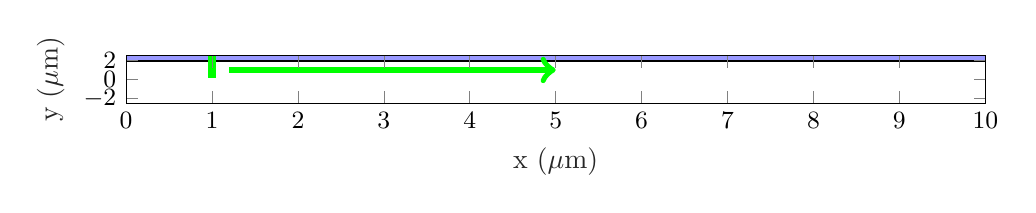
\begin{tikzpicture}
    \begin{axis}[%
width=0.9\figW,
height=0.15\figH,
at={(0\figW,0\figH)},
scale only axis,
axis on top,
xmin=0,
xmax=10,
xlabel style={font=\color{white!15!black}},
xlabel={$\text{x (}\mu\text{m)}$},
ymin=-2.5,
ymax=2.5,
ylabel style={font=\color{white!15!black}},
ylabel={$\text{y (}\mu\text{m)}$},
axis background/.style={fill=white},
]
\filldraw[fill=blue!40!white, draw=black] (0,1.95) rectangle (60,3.05);
\filldraw[fill=blue!10!white, draw=black, opacity=1] (5.2,2.5) rectangle (24.2,3.05);
\filldraw[fill=blue!10!white, draw=black, opacity=1] (35.8,2.5) rectangle (54.8,3.05);
\draw[draw=green, line width=1mm] (1,0.2) -- (1,4.8);
\draw[line width=0.8mm, draw=green, ->] (1.2,4) -- (5,4);
\draw[line width=0.8mm, draw=green, ->] (1.2,1) -- (5,1);
\end{axis}
\end{tikzpicture}
\caption[The modulated waveguide structure]{Weakly modulated waveguide structure.}
\label{fig:weakmod}
\end{figure}


\begin{figure}
    \centering
    \setlength{\figH}{1\linewidth}
	\setlength{\figW}{1\textwidth}
	\pgfplotsset{every axis/.append style={
                    label style={font=\footnotesize},
                    tick label style={font=\footnotesize}  
                    }}
    \begin{subfigure}[t]{0.5\textwidth}
		% This file was created by matlab2tikz.
%
%The latest updates can be retrieved from
%  http://www.mathworks.com/matlabcentral/fileexchange/22022-matlab2tikz-matlab2tikz
%where you can also make suggestions and rate matlab2tikz.
%
\pgfplotsset{weakMod/.style={
	width=0.32\figW,
	height=0.15\figH,
	scale only axis,
	axis on top,
	xmin=0,
	xmax=10,
	ymin=-2.5,
	ymax=2.5,
	%xlabel style={font=\color{white!15!black}},
	%ylabel style={font=\color{white!15!black}},
	axis background/.style={fill=white},
	colormap={mymap}{[1pt] rgb(0pt)=(0,0,1); rgb(31pt)=(1,1,1); rgb(32pt)=(1,1,1); rgb(63pt)=(1,0,0)},
	colorbar,
	colorbar style={width=.03\linewidth, at={(1.08,0.075\figH)}, anchor=east}
	}
}

\begin{tikzpicture}

\begin{axis}[%
weakMod,
at={(0\figW,0.92\figH)},
point meta min=-0.153883565276573,
point meta max=0.153883565276573,
xticklabels={,,},
colorbar style={title = $V / \mu m$, width=.03\linewidth, at={(1.08,0.075\figH)}, anchor=east}
]
\addplot [forget plot] graphics [xmin=0, xmax=10, ymin=-2.5, ymax=2.5] {graphs/weakmod/nameoffile2-1.png};
\draw (0,-0.5) -- (10,-0.5);
\draw (0,0.5) -- (10,0.5);
\node at (5,1.8) {$\omega_1+2\Omega$};
\end{axis}

\begin{axis}[%
weakMod,
at={(0\figW,0.69\figH)},
point meta min=-1.37640682053953,
point meta max=1.37640682053953,
xticklabels={,,}
]
\addplot [forget plot] graphics [xmin=0, xmax=10, ymin=-2.5, ymax=2.5] {graphs/weakmod/nameoffile2-2.png};
\draw (0,-0.5) -- (10,-0.5);
\draw (0,0.5) -- (10,0.5);
\node at (5,1.8) {$\omega_1+\Omega$};
\end{axis}

\begin{axis}[%
weakMod,
at={(0\figW,0.46\figH)},
point meta min=-24.7127053691998,
point meta max=24.7127053691998,
xticklabels={,,},
ylabel={$\text{y (}\mu\text{m)}$}
]
\addplot [forget plot] graphics [xmin=0, xmax=10, ymin=-2.5, ymax=2.5] {graphs/weakmod/nameoffile2-3.png};
\draw (0,-0.5) -- (10,-0.5);
\draw (0,0.5) -- (10,0.5);
\node at (5,1.8) {$\omega_1$};
\end{axis}

\begin{axis}[%
weakMod,
at={(0\figW,0.23\figH)},
point meta min=-2.69144358712869,
point meta max=2.69144358712869,
xticklabels={,,}
]
\addplot [forget plot] graphics [xmin=0, xmax=10, ymin=-2.5, ymax=2.5] {graphs/weakmod/nameoffile2-4.png};
\draw (0,-0.5) -- (10,-0.5);
\draw (0,0.5) -- (10,0.5);
\node at (5,1.8) {$\omega_1-\Omega$};
\end{axis}

\begin{axis}[%
weakMod,
at={(0\figW,0\figH)},
point meta min=-0.251011435268562,
point meta max=0.251011435268562,
%xlabel style={font=\color{white!15!black}},
xlabel={$\text{x (}\mu\text{m)}$}
]
\addplot [forget plot] graphics [xmin=0, xmax=10, ymin=-2.5, ymax=2.5] {graphs/weakmod/nameoffile2-5.png};
\draw (0,-0.5) -- (10,-0.5);
\draw (0,0.5) -- (10,0.5);
\node at (5,1.8) {$\omega_1-2\Omega$};
\end{axis}
\node at (-1,16) {\textbf{(a)}};

\end{tikzpicture}%
    \end{subfigure}%
    \begin{subfigure}[t]{0.5\textwidth}
		% This file was created by matlab2tikz.
%
%The latest updates can be retrieved from
%  http://www.mathworks.com/matlabcentral/fileexchange/22022-matlab2tikz-matlab2tikz
%where you can also make suggestions and rate matlab2tikz.
%
\definecolor{mycolor1}{rgb}{0.00000,0.44700,0.74100}%
\definecolor{mycolor2}{rgb}{0.85000,0.32500,0.09800}%
%
\begin{tikzpicture}

\begin{axis}[%
width=0.4\figW,
height=0.15\figH,
at={(0\figW,0.86\figH)},
scale only axis,
yticklabel style={/pgf/number format/fixed},
xmin=0,
xmax=10,
ymin=0,
ymax=0.01,
axis background/.style={fill=white}
]
\addplot [color=mycolor1, forget plot]
  table[row sep=crcr]{%
0	2.33105594482646e-06\\
0.025062656641604	9.01287932868077e-07\\
0.050125313283208	9.85818098486402e-07\\
0.075187969924812	2.22160020668889e-06\\
0.100250626566416	4.06160199512851e-06\\
0.12531328320802	6.42950087937509e-06\\
0.150375939849624	1.10916214092756e-05\\
0.175438596491228	2.10439751069597e-05\\
0.200501253132832	3.54210760317291e-05\\
0.225563909774436	5.29780406878314e-05\\
0.25062656641604	7.08795739166728e-05\\
0.275689223057644	8.69794532406785e-05\\
0.300751879699248	9.99914218489389e-05\\
0.325814536340852	0.000109565720725502\\
0.350877192982456	0.000116049452212893\\
0.37593984962406	0.000120143836165418\\
0.401002506265664	0.000122620411009073\\
0.426065162907268	0.000124148882176009\\
0.451127819548872	0.000125222681870323\\
0.476190476190476	0.000126147916749036\\
0.50125313283208	0.000127067392077936\\
0.526315789473684	0.000128009668166094\\
0.551378446115288	0.000128967753098669\\
0.576441102756892	0.000129933778403758\\
0.601503759398496	0.000130899863583817\\
0.6265664160401	0.000131858166573504\\
0.651629072681704	0.000132800928978526\\
0.676691729323308	0.000133720516139098\\
0.701754385964912	0.000134609452130239\\
0.726817042606516	0.000135460449843398\\
0.75187969924812	0.000136266436293182\\
0.776942355889724	0.000137020573262347\\
0.802005012531328	0.000137716273340372\\
0.827067669172932	0.00013834721132767\\
0.852130325814536	0.00013890733087038\\
0.87719298245614	0.000139390846060993\\
0.902255639097744	0.000139792237590067\\
0.927318295739348	0.000140106242868012\\
0.952380952380952	0.000140327839360965\\
0.977443609022556	0.000140452220214622\\
1.00250626566416	0.000140474761096893\\
1.02756892230576	0.000140390977109575\\
1.05263157894737	0.000140196468654413\\
1.07769423558897	0.000139886899864048\\
1.10275689223058	0.000139457817348935\\
1.12781954887218	0.000138904607386717\\
1.15288220551378	0.00013822243286992\\
1.17794486215539	0.000137406104029872\\
1.20300751879699	0.000136449978344093\\
1.2280701754386	0.000135347878247097\\
1.2531328320802	0.000134093047860769\\
1.2781954887218	0.000132678179885692\\
1.30325814536341	0.000131095557087949\\
1.32832080200501	0.0001293373709195\\
1.35338345864662	0.000127396305960184\\
1.37844611528822	0.000125266521235278\\
1.40350877192982	0.000122945239863154\\
1.42857142857143	0.00012043533754365\\
1.45363408521303	0.00011774977441503\\
1.47869674185464	0.000114919986968045\\
1.50375939849624	0.00011689735118425\\
1.52882205513784	0.000121726198197074\\
1.55388471177945	0.000125945416088278\\
1.57894736842105	0.00012901366914319\\
1.60401002506266	0.000130183898799949\\
1.62907268170426	0.000129119878082873\\
1.65413533834586	0.000125367765914451\\
1.67919799498747	0.000118418187393541\\
1.70426065162907	0.00010764709403612\\
1.72932330827068	9.33032873045091e-05\\
1.75438596491228	9.63900619751649e-05\\
1.77944862155388	0.000110162821237525\\
1.80451127819549	0.000130418484980492\\
1.82957393483709	0.000159983186532498\\
1.8546365914787	0.000195808960613232\\
1.8796992481203	0.000236540482951088\\
1.9047619047619	0.00027956112627642\\
1.92982456140351	0.000323157866680819\\
1.95488721804511	0.000365204598420651\\
1.97994987468672	0.000404685667857003\\
2.00501253132832	0.000438717165754038\\
2.03007518796993	0.000466048108460099\\
2.05513784461153	0.000485781716335755\\
2.08020050125313	0.000497491774252237\\
2.10526315789474	0.000501354784361502\\
2.13032581453634	0.000498297105971021\\
2.15538847117795	0.000490146572364364\\
2.18045112781955	0.000479747283797727\\
2.20551378446115	0.0004709292171558\\
2.23057644110276	0.000468136437728386\\
2.25563909774436	0.000475536204729574\\
2.28070175438596	0.000508573838133546\\
2.30576441102757	0.000578824528855558\\
2.33082706766917	0.000644635317553838\\
2.35588972431078	0.000703274403488717\\
2.38095238095238	0.000752486897907784\\
2.40601503759398	0.000790679207867245\\
2.43107769423559	0.000817145173476065\\
2.45614035087719	0.000856569707501827\\
2.4812030075188	0.000886797216310967\\
2.5062656641604	0.000904513602504812\\
2.53132832080201	0.000911221038418481\\
2.55639097744361	0.000907972650749936\\
2.58145363408521	0.000896810914101952\\
2.60651629072682	0.000909095163818558\\
2.63157894736842	0.00097559916637781\\
2.65664160401003	0.00106516911730901\\
2.68170426065163	0.00117339906475096\\
2.70676691729323	0.00129389534272862\\
2.73182957393484	0.00141958915119146\\
2.75689223057644	0.0015435873059353\\
2.78195488721805	0.00165964930532967\\
2.80701754385965	0.00176247113994998\\
2.83208020050125	0.00184790060122065\\
2.85714285714286	0.00191314442684713\\
2.88220551378446	0.00195698828056314\\
2.90726817042607	0.00198002856334268\\
2.93233082706767	0.00198489595925477\\
2.95739348370927	0.00197642069804736\\
2.98245614035088	0.00196163754044314\\
3.00751879699248	0.00194945694999381\\
3.03258145363409	0.00194978408580487\\
3.05764411027569	0.00197196657922211\\
3.08270676691729	0.00202281119539654\\
3.1077694235589	0.00210487416965082\\
3.1328320802005	0.0022158529497659\\
3.15789473684211	0.00234930256909349\\
3.18295739348371	0.00249617703392651\\
3.20802005012531	0.00264645909350545\\
3.23308270676692	0.00279043805836857\\
3.25814536340852	0.00291956462772439\\
3.28320802005013	0.00302699387723154\\
3.30827067669173	0.00310794776683407\\
3.33333333333333	0.00315998612400866\\
3.35839598997494	0.00318322701102628\\
3.38345864661654	0.00318051651128588\\
3.40852130325815	0.00315750737539163\\
3.43358395989975	0.0031225557882141\\
3.45864661654135	0.00308628650386694\\
3.48370927318296	0.00306064024846753\\
3.50877192982456	0.00305728376371873\\
3.53383458646617	0.00308552425865029\\
3.55889724310777	0.00315028101921426\\
3.58395989974937	0.00325091030755287\\
3.60902255639098	0.00338139878713172\\
3.63408521303258	0.00353175785505425\\
3.65914786967419	0.00368994819977774\\
3.68421052631579	0.00384368441507989\\
3.70927318295739	0.00398180618099609\\
3.734335839599	0.00409520378563325\\
3.7593984962406	0.00417741575569467\\
3.78446115288221	0.0042250208651272\\
3.80952380952381	0.00423790197874127\\
3.83458646616541	0.00421940523275858\\
3.85964912280702	0.00417636252674028\\
3.88471177944862	0.00411888336835312\\
3.90977443609023	0.00405975682519464\\
3.93483709273183	0.00401326997915466\\
3.95989974937343	0.0039933280305192\\
3.98496240601504	0.0040110433320835\\
4.01002506265664	0.00407239661915056\\
4.03508771929825	0.00417684197740548\\
4.06015037593985	0.00431745285271002\\
4.08521303258145	0.00448247946649862\\
4.11027568922306	0.00465759818907069\\
4.13533834586466	0.00482809314380862\\
4.16040100250627	0.00498055737023629\\
4.18546365914787	0.00510405520412116\\
4.21052631578947	0.00519086387114963\\
4.23558897243108	0.00523693687523052\\
4.26065162907268	0.00524218720025869\\
4.28571428571429	0.0052106262694225\\
4.31077694235589	0.00515032961228983\\
4.33583959899749	0.00507313058079394\\
4.3609022556391	0.00499387451679455\\
4.3859649122807	0.00492903458588072\\
4.41102756892231	0.00489458101555214\\
4.43609022556391	0.00490329555835201\\
4.46115288220551	0.00496217745924617\\
4.48621553884712	0.00507087017737138\\
4.51127819548872	0.00522176568056596\\
4.53634085213033	0.0054016855372274\\
4.56140350877193	0.00559438610978223\\
4.58646616541353	0.0057830453050283\\
4.61152882205514	0.00595223615488753\\
4.63659147869674	0.00608928468040229\\
4.66165413533835	0.00618512425291711\\
4.68671679197995	0.00623480330522157\\
4.71177944862155	0.00623776280564567\\
4.73684210526316	0.00619793536580277\\
4.76190476190476	0.00612365106957959\\
4.78696741854637	0.00602726793141463\\
4.81203007518797	0.0059243818487701\\
4.83709273182957	0.00583244098729512\\
4.86215538847118	0.00576865955106506\\
4.88721804511278	0.00574737200982652\\
4.91228070175439	0.00577736777763606\\
4.93734335839599	0.00586005622226308\\
4.96240601503759	0.00598918226571152\\
4.9874686716792	0.00615218840969882\\
5.0125313283208	0.00633263451882927\\
5.03759398496241	0.006512835608889\\
5.06265664160401	0.00667610405149375\\
5.08771929824561	0.00680836841104387\\
5.11278195488722	0.00689921369358982\\
5.13784461152882	0.00694248724948097\\
5.16290726817043	0.00693660245854957\\
5.18796992481203	0.00688461664634955\\
5.21303258145363	0.00679409524218169\\
5.23809523809524	0.00667671095182401\\
5.26315789473684	0.00654746990512588\\
5.28822055137845	0.00642342627658592\\
5.31328320802005	0.006321790187222\\
5.33834586466165	0.00625751155473984\\
5.36340852130326	0.00624073870260606\\
5.38847117794486	0.0062748528299855\\
5.41353383458647	0.00635578603965757\\
5.43859649122807	0.00647289789875069\\
5.46365914786967	0.006611057994961\\
5.48872180451128	0.00675320385431907\\
5.51378446115288	0.00688270460996791\\
5.53884711779449	0.0069851780539107\\
5.56390977443609	0.00704970824293168\\
5.58897243107769	0.00706956589175394\\
5.6140350877193	0.00704256185138169\\
5.6390977443609	0.00697112631075445\\
5.66416040100251	0.00686214703909596\\
5.68922305764411	0.00672653818813961\\
5.71428571428571	0.00657845632286919\\
5.73934837092732	0.0064340507445138\\
5.76441102756892	0.00630967078536936\\
5.78947368421053	0.00621960512878739\\
5.81453634085213	0.00617370337836586\\
5.83959899749373	0.00617550408062541\\
5.86466165413534	0.00622152287021823\\
5.88972431077694	0.00630199287272465\\
5.91478696741855	0.00640278057071442\\
5.93984962406015	0.00650781763343823\\
5.96491228070175	0.0066014015995744\\
5.98997493734336	0.00666999467532613\\
6.01503759398496	0.00670343899062142\\
6.04010025062657	0.00669567072787964\\
6.06516290726817	0.00664505542404895\\
6.09022556390977	0.00655443616921541\\
6.11528822055138	0.00643092935455121\\
6.14035087719298	0.00628544076297387\\
6.16541353383459	0.00613182071478735\\
6.19047619047619	0.00598555279020764\\
6.21553884711779	0.00586191981279322\\
6.2406015037594	0.005773762453455\\
6.265664160401	0.00572922914995713\\
6.29072681704261	0.00573015955124683\\
6.31578947368421	0.00577169994871782\\
6.34085213032582	0.0058433233590717\\
6.36591478696742	0.00593086965594827\\
6.39097744360902	0.00601892222660684\\
6.41604010025063	0.00609293143563099\\
6.44110275689223	0.00614079569530174\\
6.46616541353383	0.00615387634928766\\
6.49122807017544	0.00612755183297259\\
6.51629072681704	0.00606143286901172\\
6.54135338345865	0.00595932004080523\\
6.56641604010025	0.00582892647334148\\
6.59147869674185	0.00568132877927012\\
6.61654135338346	0.00553006093660052\\
6.64160401002506	0.00538975469695613\\
6.66666666666667	0.00527429412836912\\
6.69172932330827	0.00519466235518487\\
6.71679197994987	0.00515692496770333\\
6.74185463659148	0.00516099026368992\\
6.76691729323308	0.0052006419904761\\
6.79197994987469	0.0052648537361007\\
6.81704260651629	0.00533988970443366\\
6.84210526315789	0.00541152066077952\\
6.8671679197995	0.00546686506077676\\
6.8922305764411	0.00549567070407255\\
6.91729323308271	0.00549107363896754\\
6.94235588972431	0.00544995601952891\\
6.96741854636591	0.00537301704813567\\
6.99248120300752	0.0052646249865989\\
7.01754385964912	0.00513246401303426\\
7.04260651629073	0.00498693969184507\\
7.06766917293233	0.00484027153067527\\
7.09273182957393	0.00470520411728246\\
7.11779448621554	0.00459334871743802\\
7.14285714285714	0.00451335016927559\\
7.16791979949875	0.00446930425251259\\
7.19298245614035	0.00445995671113169\\
7.21804511278195	0.00447902426986659\\
7.24310776942356	0.00451654079464245\\
7.26817042606516	0.00456074658005731\\
7.29323308270677	0.0045999581210645\\
7.31829573934837	0.00462404796940946\\
7.34335839598998	0.00462542092152954\\
7.36842105263158	0.00459954020696279\\
7.39348370927318	0.00454511143766498\\
7.41854636591479	0.00446401589936052\\
7.44360902255639	0.00436104239668221\\
7.468671679198	0.00424342284701873\\
7.4937343358396	0.00412014372133984\\
7.5187969924812	0.00400099707659422\\
7.54385964912281	0.00389696551379262\\
7.56892230576441	0.003818399802297\\
7.59398496240602	0.00377056049898826\\
7.61904761904762	0.00375214645604881\\
7.64411027568922	0.00375886691552815\\
7.66917293233083	0.00377836534510917\\
7.69423558897243	0.00380384100840521\\
7.71929824561404	0.00382569969103262\\
7.74436090225564	0.00383704058820069\\
7.76942355889724	0.00383366622303628\\
7.79448621553885	0.00381422914294992\\
7.81954887218045	0.00377959149280756\\
7.84461152882206	0.00373174625278672\\
7.86967418546366	0.00367532986717069\\
7.89473684210526	0.00361632364176862\\
7.91979949874687	0.00356124002735666\\
7.94486215538847	0.0035161548192967\\
7.96992481203008	0.00348743510061064\\
7.99498746867168	0.00347628062808456\\
8.02005012531328	0.00348199982076393\\
8.04511278195489	0.0035016179796379\\
8.07017543859649	0.00353029797720339\\
8.09523809523809	0.00356240462312989\\
8.1203007518797	0.00359260700069798\\
8.1453634085213	0.00361505297161921\\
8.17042606516291	0.00362653009861709\\
8.19548872180451	0.00362707498586391\\
8.22055137844612	0.00361678079425638\\
8.24561403508772	0.00359828898685418\\
8.27067669172932	0.00357578480748705\\
8.29573934837093	0.00355640285854321\\
8.32080200501253	0.00354572101451394\\
8.34586466165413	0.00354811424349544\\
8.37092731829574	0.00356710673404792\\
8.39598997493734	0.00360320911718777\\
8.42105263157895	0.00365300404515562\\
8.44611528822055	0.00371348452377955\\
8.47117794486216	0.00377754307586727\\
8.49624060150376	0.00383968711902125\\
8.52130325814536	0.00389487578850262\\
8.54636591478697	0.00393840836841639\\
8.57142857142857	0.0039677665061839\\
8.59649122807017	0.00398227547934529\\
8.62155388471178	0.00398319764205871\\
8.64661654135338	0.00397362587259964\\
8.67167919799499	0.0039581690380815\\
8.69674185463659	0.00394257464154704\\
8.7218045112782	0.00393267173782798\\
8.7468671679198	0.00393372219093863\\
8.7719298245614	0.00394964408050319\\
8.79699248120301	0.0039823224937534\\
8.82205513784461	0.00403133106929003\\
8.84711779448622	0.00409408837193421\\
8.87218045112782	0.00416639975128865\\
8.89724310776942	0.00424323426147012\\
8.92230576441103	0.00431955449086212\\
8.94736842105263	0.00439104909657322\\
8.97243107769424	0.00445467668972892\\
8.99749373433584	0.00450898259423882\\
9.02255639097744	0.00455418774034772\\
9.04761904761905	0.00459308451401953\\
9.07268170426065	0.00462656041265752\\
9.09774436090226	0.00465526507371267\\
9.12280701754386	0.00467971782823716\\
9.14786967418546	0.00470035370945958\\
9.17293233082707	0.00471754554055014\\
9.19799498746867	0.0047316163258144\\
9.22305764411028	0.00474284748658796\\
9.24812030075188	0.00475148520053658\\
9.27318295739348	0.00475774576985989\\
9.29824561403509	0.00476182037991059\\
9.32330827067669	0.0047638793722978\\
9.3483709273183	0.00476407606407492\\
9.3734335839599	0.00476255011683106\\
9.3984962406015	0.0047594304590336\\
9.42355889724311	0.00475483777407944\\
9.44862155388471	0.00474888657700054\\
9.47368421052632	0.00474168691119497\\
9.49874686716792	0.00473334570185936\\
9.52380952380952	0.00472396780505595\\
9.54887218045113	0.00471362747359175\\
9.57393483709273	0.00470110876284084\\
9.59899749373434	0.00468101850979356\\
9.62406015037594	0.00464195578533996\\
9.64912280701754	0.00456559384554575\\
9.67418546365915	0.00442704948796863\\
9.69924812030075	0.00419757401590522\\
9.72431077694236	0.00385082001791481\\
9.74937343358396	0.00337320968824328\\
9.77443609022556	0.00277653553046559\\
9.79949874686717	0.00210697566448238\\
9.82456140350877	0.00144168749763041\\
9.84962406015038	0.000867130180653859\\
9.87468671679198	0.000445404109844512\\
9.89974937343358	0.000189039114030387\\
9.92481203007519	6.37383173478161e-05\\
9.94987468671679	1.99535854235737e-05\\
9.9749373433584	1.19083138010841e-05\\
10	5.9947246446025e-06\\
};
\addplot [color=mycolor2, forget plot]
  table[row sep=crcr]{%
1.5	0\\
1.51	0\\
1.52	2.02337787537816e-07\\
1.53	6.07001884896979e-07\\
1.54	1.21396921427095e-06\\
1.55	2.02320509907986e-06\\
1.56	3.03466326595137e-06\\
1.57	4.24828584736569e-06\\
1.58	5.66400338496448e-06\\
1.59	7.28173483352348e-06\\
1.6	9.10138756558876e-06\\
1.61	1.11228573767761e-05\\
1.62	1.33460284917337e-05\\
1.63	1.57707735707668e-05\\
1.64	1.83969537171259e-05\\
1.65	2.12244184849553e-05\\
1.66	2.42530058879047e-05\\
1.67	2.74825424084003e-05\\
1.68	3.09128430075778e-05\\
1.69	3.45437111358743e-05\\
1.7	3.83749387442801e-05\\
1.71	4.24063062962493e-05\\
1.72	4.66375827802682e-05\\
1.73	5.10685257230813e-05\\
1.74	5.56988812035743e-05\\
1.75	6.05283838673127e-05\\
1.76	6.55567569417352e-05\\
1.77	7.07837122520029e-05\\
1.78	7.62089502374998e-05\\
1.79	8.18321599689882e-05\\
1.8	8.76530191664136e-05\\
1.81	9.36711942173621e-05\\
1.82	9.98863401961661e-05\\
1.83	0.000106298100883659\\
1.84	0.000112906108787579\\
1.85	0.000119709985163616\\
1.86	0.000126709340037108\\
1.87	0.000133903772225375\\
1.88	0.000141292869360706\\
1.89	0.000148876207913979\\
1.9	0.000156653353218922\\
1.91	0.000164623859497019\\
1.92	0.000172787269883049\\
1.93	0.000181143116451259\\
1.94	0.000189690920242178\\
1.95	0.000198430191290062\\
1.96	0.000207360428650969\\
1.97	0.000216481120431464\\
1.98	0.000225791743817957\\
1.99	0.000235291765106667\\
2	0.000244980639734206\\
2.01	0.000254857812308795\\
2.02	0.000264922716642095\\
2.03	0.000275174775781668\\
2.04	0.000285613402044044\\
2.05	0.000296237997048415\\
2.06	0.000307047951750941\\
2.07	0.000318042646479667\\
2.08	0.000329221450970056\\
2.09	0.000340583724401127\\
2.1	0.000352128815432202\\
2.11	0.00036385606224026\\
2.12	0.00037576479255789\\
2.13	0.000387854323711854\\
2.14	0.000400123962662238\\
2.15	0.000412573006042207\\
2.16	0.000425200740198357\\
2.17	0.000438006441231654\\
2.18	0.000450989375038963\\
2.19	0.000464148797355176\\
2.2	0.000477483953795912\\
2.21	0.000490994079900807\\
2.22	0.000504678401177392\\
2.23	0.000518536133145534\\
2.24	0.000532566481382471\\
2.25	0.000546768641568409\\
2.26	0.000561141799532695\\
2.27	0.000575685131300558\\
2.28	0.000590397803140422\\
2.29	0.000605278971611772\\
2.3	0.000620327783613591\\
2.31	0.000635543376433355\\
2.32	0.000650924877796576\\
2.33	0.00066647140591691\\
2.34	0.000682182069546807\\
2.35	0.000698055968028713\\
2.36	0.000714092191346815\\
2.37	0.000730289820179331\\
2.38	0.00074664792595134\\
2.39	0.000763165570888143\\
2.4	0.000779841808069164\\
2.41	0.000796675681482383\\
2.42	0.000813666226079287\\
2.43	0.000830812467830359\\
2.44	0.000848113423781083\\
2.45	0.000865568102108461\\
2.46	0.000883175502178061\\
2.47	0.000900934614601566\\
2.48	0.000918844421294838\\
2.49	0.000936903895536485\\
2.5	0.000955112002026935\\
2.51	0.000973467696948009\\
2.52	0.000991969928022991\\
2.53	0.00101061763457719\\
2.54	0.00102940974759901\\
2.55	0.00104834518980144\\
2.56	0.00106742287568417\\
2.57	0.001086641711596\\
2.58	0.00110600059579789\\
2.59	0.00112549841852638\\
2.6	0.00114513406205756\\
2.61	0.00116490640077141\\
2.62	0.00118481430121669\\
2.63	0.00120485662217626\\
2.64	0.00122503221473285\\
2.65	0.00124533992233528\\
2.66	0.00126577858086515\\
2.67	0.00128634701870395\\
2.68	0.00130704405680062\\
2.69	0.0013278685087396\\
2.7	0.00134881918080919\\
2.71	0.00136989487207049\\
2.72	0.00139109437442667\\
2.73	0.00141241647269269\\
2.74	0.00143385994466544\\
2.75	0.0014554235611943\\
2.76	0.00147710608625213\\
2.77	0.00149890627700661\\
2.78	0.00152082288389206\\
2.79	0.0015428546506816\\
2.8	0.00156500031455977\\
2.81	0.00158725860619546\\
2.82	0.00160962824981529\\
2.83	0.00163210796327738\\
2.84	0.00165469645814548\\
2.85	0.00167739243976346\\
2.86	0.0017001946073302\\
2.87	0.00172310165397485\\
2.88	0.00174611226683247\\
2.89	0.00176922512711996\\
2.9	0.00179243891021245\\
2.91	0.00181575228571997\\
2.92	0.00183916391756448\\
2.93	0.00186267246405729\\
2.94	0.00188627657797676\\
2.95	0.00190997490664637\\
2.96	0.00193376609201313\\
2.97	0.00195764877072632\\
2.98	0.00198162157421649\\
2.99	0.00200568312877489\\
3	0.00202983205563314\\
3.01	0.00205406697104321\\
3.02	0.00207838648635776\\
3.03	0.00210278920811074\\
3.04	0.00212727373809828\\
3.05	0.00215183867345994\\
3.06	0.00217648260676019\\
3.07	0.00220120412607016\\
3.08	0.00222600181504976\\
3.09	0.00225087425303\\
3.1	0.00227582001509559\\
3.11	0.00230083767216785\\
3.12	0.00232592579108786\\
3.13	0.00235108293469986\\
3.14	0.00237630766193494\\
3.15	0.00240159852789491\\
3.16	0.00242695408393654\\
3.17	0.0024523728777559\\
3.18	0.00247785345347305\\
3.19	0.0025033943517169\\
3.2	0.00252899410971035\\
3.21	0.00255465126135558\\
3.22	0.00258036433731965\\
3.23	0.00260613186512025\\
3.24	0.0026319523692117\\
3.25	0.00265782437107112\\
3.26	0.00268374638928485\\
3.27	0.00270971693963502\\
3.28	0.00273573453518636\\
3.29	0.00276179768637315\\
3.3	0.00278790490108641\\
3.31	0.0028140546847612\\
3.32	0.00284024554046419\\
3.33	0.0028664759689813\\
3.34	0.00289274446890558\\
3.35	0.00291904953672522\\
3.36	0.00294538966691172\\
3.37	0.00297176335200822\\
3.38	0.00299816908271797\\
3.39	0.00302460534799298\\
3.4	0.00305107063512273\\
3.41	0.00307756342982309\\
3.42	0.00310408221632535\\
3.43	0.00313062547746536\\
3.44	0.00315719169477279\\
3.45	0.00318377934856054\\
3.46	0.00321038691801422\\
3.47	0.00323701288128177\\
3.48	0.00326365571556318\\
3.49	0.00329031389720025\\
3.5	0.00331698590176655\\
3.51	0.00334367020415738\\
3.52	0.00337036527867985\\
3.53	0.00339706959914304\\
3.54	0.00342378163894823\\
3.55	0.0034504998711792\\
3.56	0.00347722276869261\\
3.57	0.00350394880420842\\
3.58	0.00353067645040039\\
3.59	0.0035574041799866\\
3.6	0.00358413046582007\\
3.61	0.00361085378097937\\
3.62	0.00363757259885931\\
3.63	0.00366428539326163\\
3.64	0.00369099063848577\\
3.65	0.0037176868094196\\
3.66	0.00374437238163023\\
3.67	0.0037710458314548\\
3.68	0.00379770563609129\\
3.69	0.00382435027368937\\
3.7	0.0038509782234412\\
3.71	0.00387758796567227\\
3.72	0.00390417798193222\\
3.73	0.00393074675508564\\
3.74	0.00395729276940287\\
3.75	0.00398381451065079\\
3.76	0.00401031046618356\\
3.77	0.00403677912503336\\
3.78	0.00406321897800109\\
3.79	0.00408962851774698\\
3.8	0.00411600623888128\\
3.81	0.0041423506380548\\
3.82	0.00416866021404942\\
3.83	0.00419493346786858\\
3.84	0.00422116890282769\\
3.85	0.00424736502464449\\
3.86	0.00427352034152931\\
3.87	0.00429963336427532\\
3.88	0.00432570260634862\\
3.89	0.00435172658397835\\
3.9	0.00437770381624662\\
3.91	0.00440363282517846\\
3.92	0.00442951213583156\\
3.93	0.00445534027638597\\
3.94	0.00448111577823376\\
3.95	0.00450683717606846\\
3.96	0.00453250300797447\\
3.97	0.00455811181551634\\
3.98	0.00458366214382792\\
3.99	0.00460915254170141\\
4	0.00463458156167626\\
4.01	0.00465994776012798\\
4.02	0.00468524969735677\\
4.03	0.00471048593767605\\
4.04	0.00473565504950082\\
4.05	0.00476075560543594\\
4.06	0.00478578618236415\\
4.07	0.00481074536153404\\
4.08	0.00483563172864784\\
4.09	0.00486044387394899\\
4.1	0.00488518039230963\\
4.11	0.00490983988331788\\
4.12	0.00493442095136494\\
4.13	0.00495892220573204\\
4.14	0.00498334226067722\\
4.15	0.00500767973552186\\
4.16	0.00503193325473711\\
4.17	0.0050561014480301\\
4.18	0.00508018295042992\\
4.19	0.00510417640237345\\
4.2	0.00512808044979098\\
4.21	0.00515189374419161\\
4.22	0.00517561494274846\\
4.23	0.00519924270838365\\
4.24	0.00522277570985308\\
4.25	0.00524621262183102\\
4.26	0.00526955212499439\\
4.27	0.00529279290610696\\
4.28	0.00531593365810316\\
4.29	0.00533897308017177\\
4.3	0.00536190987783936\\
4.31	0.00538474276305345\\
4.32	0.00540747045426548\\
4.33	0.0054300916765135\\
4.34	0.00545260516150463\\
4.35	0.00547500964769726\\
4.36	0.00549730388038305\\
4.37	0.00551948661176858\\
4.38	0.0055415566010568\\
4.39	0.00556351261452824\\
4.4	0.00558535342562191\\
4.41	0.00560707781501597\\
4.42	0.00562868457070806\\
4.43	0.00565017248809548\\
4.44	0.00567154037005498\\
4.45	0.00569278702702232\\
4.46	0.00571391127707158\\
4.47	0.0057349119459941\\
4.48	0.00575578786737726\\
4.49	0.00577653788268284\\
4.5	0.00579716084132517\\
4.51	0.005817655600749\\
4.52	0.005838021026507\\
4.53	0.00585825599233705\\
4.54	0.00587835938023914\\
4.55	0.00589833008055206\\
4.56	0.00591816699202975\\
4.57	0.00593786902191728\\
4.58	0.00595743508602664\\
4.59	0.00597686410881214\\
4.6	0.0059961550234455\\
4.61	0.00601530677189069\\
4.62	0.00603431830497835\\
4.63	0.00605318858248002\\
4.64	0.00607191657318193\\
4.65	0.00609050125495853\\
4.66	0.00610894161484574\\
4.67	0.00612723664911376\\
4.68	0.00614538536333968\\
4.69	0.00616338677247965\\
4.7	0.00618123990094082\\
4.71	0.0061989437826529\\
4.72	0.00621649746113939\\
4.73	0.00623389998958846\\
4.74	0.00625115043092357\\
4.75	0.00626824785787367\\
4.76	0.00628519135304312\\
4.77	0.00630198000898125\\
4.78	0.00631861292825157\\
4.79	0.00633508922350069\\
4.8	0.00635140801752684\\
4.81	0.00636756844334812\\
4.82	0.00638356964427031\\
4.83	0.00639941077395445\\
4.84	0.00641509099648401\\
4.85	0.00643060948643174\\
4.86	0.00644596542892615\\
4.87	0.0064611580197177\\
4.88	0.00647618646524458\\
4.89	0.00649104998269821\\
4.9	0.00650574780008837\\
4.91	0.00652027915630796\\
4.92	0.00653464330119747\\
4.93	0.00654883949560904\\
4.94	0.00656286701147024\\
4.95	0.0065767251318475\\
4.96	0.0065904131510091\\
4.97	0.00660393037448799\\
4.98	0.0066172761191441\\
4.99	0.00663044971322641\\
5	0.00664345049643463\\
5.01	0.00665627781998058\\
5.02	0.00666893104664919\\
5.03	0.00668140955085917\\
5.04	0.00669371271872338\\
5.05	0.00670583994810877\\
5.06	0.00671779064869613\\
5.07	0.00672956424203934\\
5.08	0.00674116016162442\\
5.09	0.00675257785292814\\
5.1	0.0067638167734764\\
5.11	0.00677487639290219\\
5.12	0.0067857561930033\\
5.13	0.00679645566779961\\
5.14	0.00680697432359016\\
5.15	0.00681731167900981\\
5.16	0.00682746726508562\\
5.17	0.00683744062529289\\
5.18	0.00684723131561092\\
5.19	0.0068568389045784\\
5.2	0.00686626297334853\\
5.21	0.00687550311574378\\
5.22	0.00688455893831039\\
5.23	0.00689343006037257\\
5.24	0.00690211611408631\\
5.25	0.00691061674449297\\
5.26	0.00691893160957259\\
5.27	0.00692706038029677\\
5.28	0.00693500274068141\\
5.29	0.00694275838783909\\
5.3	0.00695032703203114\\
5.31	0.00695770839671944\\
5.32	0.00696490221861799\\
5.33	0.00697190824774412\\
5.34	0.00697872624746948\\
5.35	0.00698535599457074\\
5.36	0.00699179727928\\
5.37	0.00699804990533498\\
5.38	0.00700411369002891\\
5.39	0.00700998846426019\\
5.4	0.00701567407258175\\
5.41	0.00702117037325023\\
5.42	0.00702647723827483\\
5.43	0.00703159455346602\\
5.44	0.00703652221848388\\
5.45	0.00704126014688634\\
5.46	0.00704580826617708\\
5.47	0.0070501665178533\\
5.48	0.00705433485745319\\
5.49	0.0070583132546032\\
5.5	0.00706210169306515\\
5.51	0.00706570017078306\\
5.52	0.00706910869992983\\
5.53	0.00707232730695368\\
5.54	0.00707535603262444\\
5.55	0.00707819493207962\\
5.56	0.00708084407487026\\
5.57	0.00708330354500674\\
5.58	0.00708557344100421\\
5.59	0.00708765387592803\\
5.6	0.00708954497743896\\
5.61	0.00709124688783818\\
5.62	0.00709275976411222\\
5.63	0.00709408377797768\\
5.64	0.00709521911592581\\
5.65	0.00709616597926703\\
5.66	0.00709692458417517\\
5.67	0.00709749516173175\\
5.68	0.00709787795796999\\
5.69	0.00709807323391883\\
5.7	0.0070980812656467\\
5.71	0.00709790234430532\\
5.72	0.00709753677617331\\
5.73	0.00709698488269972\\
5.74	0.00709624700054748\\
5.75	0.0070953234816368\\
5.76	0.00709421469318837\\
5.77	0.00709292101776664\\
5.78	0.00709144285332289\\
5.79	0.00708978061323835\\
5.8	0.00708793472636716\\
5.81	0.00708590563707933\\
5.82	0.00708369380530366\\
5.83	0.00708129970657053\\
5.84	0.00707872383205479\\
5.85	0.00707596668861843\\
5.86	0.00707302879885339\\
5.87	0.00706991070112422\\
5.88	0.00706661294961079\\
5.89	0.00706313611435089\\
5.9	0.00705948078128294\\
5.91	0.00705564755228855\\
5.92	0.00705163704523514\\
5.93	0.00704744989401858\\
5.94	0.00704308674860573\\
5.95	0.00703854827507706\\
5.96	0.00703383515566924\\
5.97	0.00702894808881769\\
5.98	0.00702388778919923\\
5.99	0.00701865498777462\\
6	0.00701325043183118\\
6.01	0.00700767488502539\\
6.02	0.00700192912742548\\
6.03	0.00699601395555408\\
6.04	0.00698993018243078\\
6.05	0.00698367863761475\\
6.06	0.0069772601672474\\
6.07	0.00697067563409496\\
6.08	0.00696392591759107\\
6.09	0.00695701191387942\\
6.1	0.00694993453585631\\
6.11	0.00694269471321321\\
6.12	0.00693529339247934\\
6.13	0.00692773153706415\\
6.14	0.00692001012729985\\
6.15	0.0069121301604838\\
6.16	0.00690409265092091\\
6.17	0.00689589862996599\\
6.18	0.006887549146066\\
6.19	0.00687904526480219\\
6.2	0.00687038806893222\\
6.21	0.0068615786584321\\
6.22	0.00685261815053807\\
6.23	0.00684350767978827\\
6.24	0.00683424839806434\\
6.25	0.00682484147463277\\
6.26	0.00681528809618612\\
6.27	0.00680558946688398\\
6.28	0.00679574680839372\\
6.29	0.00678576135993101\\
6.3	0.00677563437829999\\
6.31	0.0067653671379332\\
6.32	0.00675496093093111\\
6.33	0.00674441706710137\\
6.34	0.00673373687399755\\
6.35	0.00672292169695754\\
6.36	0.00671197289914147\\
6.37	0.00670089186156905\\
6.38	0.00668967998315647\\
6.39	0.00667833868075265\\
6.4	0.00666686938917487\\
6.41	0.00665527356124374\\
6.42	0.00664355266781743\\
6.43	0.00663170819782513\\
6.44	0.00661974165829968\\
6.45	0.00660765457440932\\
6.46	0.00659544848948847\\
6.47	0.00658312496506755\\
6.48	0.00657068558090165\\
6.49	0.00655813193499819\\
6.5	0.00654546564364317\\
6.51	0.00653268834142635\\
6.52	0.00651980168126491\\
6.53	0.00650680733442573\\
6.54	0.00649370699054613\\
6.55	0.00648050235765295\\
6.56	0.00646719516218002\\
6.57	0.00645378714898369\\
6.58	0.00644028008135651\\
6.59	0.00642667574103896\\
6.6	0.00641297592822891\\
6.61	0.00639918246158898\\
6.62	0.00638529717825148\\
6.63	0.00637132193382083\\
6.64	0.00635725860237349\\
6.65	0.00634310907645504\\
6.66	0.00632887526707443\\
6.67	0.00631455910369521\\
6.68	0.00630016253422361\\
6.69	0.00628568752499325\\
6.7	0.00627113606074641\\
6.71	0.00625651014461167\\
6.72	0.00624181179807768\\
6.73	0.006227043060963\\
6.74	0.00621220599138173\\
6.75	0.0061973026657048\\
6.76	0.00618233517851672\\
6.77	0.00616730564256755\\
6.78	0.00615221618871989\\
6.79	0.00613706896589078\\
6.8	0.00612186614098813\\
6.81	0.00610660989884155\\
6.82	0.00609130244212739\\
6.83	0.00607594599128755\\
6.84	0.00606054278444215\\
6.85	0.00604509507729543\\
6.86	0.00602960514303491\\
6.87	0.00601407527222344\\
6.88	0.00599850777268376\\
6.89	0.00598290496937553\\
6.9	0.00596726920426435\\
6.91	0.00595160283618248\\
6.92	0.00593590824068111\\
6.93	0.00592018780987376\\
6.94	0.00590444395227044\\
6.95	0.00588867909260244\\
6.96	0.00587289567163726\\
6.97	0.00585709614598341\\
6.98	0.00584128298788471\\
6.99	0.00582545868500388\\
7	0.00580962574019482\\
7.01	0.00579378667126353\\
7.02	0.00577794401071707\\
7.03	0.0057621003055003\\
7.04	0.00574625811672009\\
7.05	0.00573042001935647\\
7.06	0.00571458860196058\\
7.07	0.00569876646633878\\
7.08	0.00568295622722278\\
7.09	0.00566716051192529\\
7.1	0.00565138195998077\\
7.11	0.00563562322277111\\
7.12	0.00561988696313557\\
7.13	0.00560417585496483\\
7.14	0.00558849258277875\\
7.15	0.00557283984128727\\
7.16	0.00555722033493443\\
7.17	0.00554163677742477\\
7.18	0.00552609189123204\\
7.19	0.00551058840708974\\
7.2	0.00549512906346316\\
7.21	0.00547971660600259\\
7.22	0.00546435378697743\\
7.23	0.00544904336469075\\
7.24	0.00543378810287421\\
7.25	0.00541859077006285\\
7.26	0.00540345413894958\\
7.27	0.00538838098571915\\
7.28	0.00537337408936125\\
7.29	0.00535843623096262\\
7.3	0.00534357019297799\\
7.31	0.00532877875847954\\
7.32	0.00531406471038492\\
7.33	0.00529943083066356\\
7.34	0.00528487989952125\\
7.35	0.0052704146945629\\
7.36	0.00525603798993345\\
7.37	0.00524175255543695\\
7.38	0.0052275611556338\\
7.39	0.00521346654891628\\
7.4	0.00519947148656239\\
7.41	0.00518557871176824\\
7.42	0.00517179095865917\\
7.43	0.00515811095127968\\
7.44	0.00514454140256273\\
7.45	0.0051310850132784\\
7.46	0.0051177444709626\\
7.47	0.00510452244882599\\
7.48	0.00509142160464369\\
7.49	0.00507844457962638\\
7.5	0.00506559399727319\\
7.51	0.00505287246220712\\
7.52	0.00504028255899366\\
7.53	0.00502782685094337\\
7.54	0.00501550787889909\\
7.55	0.00500332816000879\\
7.56	0.00499129018648492\\
7.57	0.0049793964243512\\
7.58	0.0049676493121778\\
7.59	0.00495605125980625\\
7.6	0.00494460464706489\\
7.61	0.00493331182247636\\
7.62	0.00492217510195811\\
7.63	0.00491119676751753\\
7.64	0.00490037906594279\\
7.65	0.00488972420749101\\
7.66	0.0048792343645751\\
7.67	0.00486891167045092\\
7.68	0.00485875821790616\\
7.69	0.00484877605795272\\
7.7	0.0048389671985241\\
7.71	0.00482933360317967\\
7.72	0.00481987718981734\\
7.73	0.00481059982939656\\
7.74	0.0048015033446734\\
7.75	0.00479258950894949\\
7.76	0.00478386004483669\\
7.77	0.00477531662303944\\
7.78	0.0047669608611565\\
7.79	0.00475879432250407\\
7.8	0.00475081851496219\\
7.81	0.00474303488984629\\
7.82	0.0047354448408057\\
7.83	0.00472804970275112\\
7.84	0.00472085075081283\\
7.85	0.00471384919933147\\
7.86	0.00470704620088322\\
7.87	0.00470044284534118\\
7.88	0.00469404015897463\\
7.89	0.00468783910358786\\
7.9	0.00468184057570038\\
7.91	0.00467604540576977\\
7.92	0.00467045435745908\\
7.93	0.00466506812694996\\
7.94	0.00465988734230306\\
7.95	0.00465491256286699\\
7.96	0.00465014427873703\\
7.97	0.00464558291026489\\
7.98	0.00464122880762036\\
7.99	0.00463708225040613\\
8	0.00463314344732632\\
8.01	0.00462941253590985\\
8.02	0.00462588958228907\\
8.03	0.00462257458103431\\
8.04	0.0046194674550449\\
8.05	0.00461656805549695\\
8.06	0.00461387616184807\\
8.07	0.00461139148189934\\
8.08	0.00460911365191443\\
8.09	0.00460704223679582\\
8.1	0.00460517673031795\\
8.11	0.00460351655541692\\
8.12	0.00460206106453643\\
8.13	0.00460080954002934\\
8.14	0.00459976119461423\\
8.15	0.00459891517188625\\
8.16	0.00459827054688138\\
8.17	0.00459782632669319\\
8.18	0.004597581451141\\
8.19	0.00459753479348835\\
8.2	0.00459768516121053\\
8.21	0.00459803129680988\\
8.22	0.00459857187867743\\
8.23	0.00459930552199942\\
8.24	0.00460023077970717\\
8.25	0.00460134614346871\\
8.26	0.0046026500447204\\
8.27	0.00460414085573695\\
8.28	0.00460581689073796\\
8.29	0.00460767640702919\\
8.3	0.00460971760617667\\
8.31	0.00461193863521184\\
8.32	0.00461433758786567\\
8.33	0.00461691250582989\\
8.34	0.00461966138004335\\
8.35	0.00462258215200154\\
8.36	0.00462567271508726\\
8.37	0.00462893091592048\\
8.38	0.00463235455572542\\
8.39	0.00463594139171283\\
8.4	0.00463968913847563\\
8.41	0.00464359546939578\\
8.42	0.00464765801806071\\
8.43	0.00465187437968722\\
8.44	0.00465624211255112\\
8.45	0.00466075873942077\\
8.46	0.00466542174899265\\
8.47	0.00467022859732747\\
8.48	0.00467517670928475\\
8.49	0.00468026347995468\\
8.5	0.0046854862760853\\
8.51	0.00469084243750364\\
8.52	0.00469632927852935\\
8.53	0.00470194408937934\\
8.54	0.0047076841375621\\
8.55	0.00471354666926036\\
8.56	0.00471952891070091\\
8.57	0.00472562806951039\\
8.58	0.00473184133605584\\
8.59	0.00473816588476912\\
8.6	0.00474459887545404\\
8.61	0.00475113745457537\\
8.62	0.00475777875652892\\
8.63	0.00476451990489168\\
8.64	0.00477135801365152\\
8.65	0.00477829018841563\\
8.66	0.00478531352759704\\
8.67	0.00479242512357886\\
8.68	0.00479962206385545\\
8.69	0.00480690143215033\\
8.7	0.00481426030951027\\
8.71	0.0048216957753753\\
8.72	0.00482920490862433\\
8.73	0.00483678478859607\\
8.74	0.00484443249608526\\
8.75	0.00485214511431376\\
8.76	0.00485991972987672\\
8.77	0.00486775343366355\\
8.78	0.0048756433217537\\
8.79	0.00488358649628744\\
8.8	0.0048915800663115\\
8.81	0.0048996211485997\\
8.82	0.00490770686844886\\
8.83	0.00491583436044994\\
8.84	0.00492400076923469\\
8.85	0.00493220325019811\\
8.86	0.00494043897019675\\
8.87	0.00494870510822338\\
8.88	0.00495699885605808\\
8.89	0.00496531741889622\\
8.9	0.00497365801595362\\
8.91	0.00498201788104912\\
8.92	0.00499039426316516\\
8.93	0.0049987844269865\\
8.94	0.00500718565341763\\
8.95	0.0050155952400792\\
8.96	0.00502401050178388\\
8.97	0.00503242877099213\\
8.98	0.0050408473982482\\
8.99	0.00504926375259694\\
9	0.00505767522198164\\
};
\end{axis}

\begin{axis}[%
width=0.4\figW,
height=0.15\figH,
at={(0\figW,0.645\figH)},
scale only axis,
yticklabel style={/pgf/number format/fixed},
xmin=0,
xmax=10,
ymin=0,
ymax=0.1,
axis background/.style={fill=white}
]
\addplot [color=mycolor1, forget plot]
  table[row sep=crcr]{%
0	6.74317351257218e-05\\
0.025062656641604	1.85705120703021e-05\\
0.050125313283208	9.00038819074966e-05\\
0.075187969924812	0.000175071168892688\\
0.100250626566416	0.00028363634279439\\
0.12531328320802	0.000413275278926579\\
0.150375939849624	0.000751284973089269\\
0.175438596491228	0.00128982609602749\\
0.200501253132832	0.00195099498707513\\
0.225563909774436	0.00265809504335846\\
0.25062656641604	0.0033280444098044\\
0.275689223057644	0.00389796536577735\\
0.300751879699248	0.00433725448811785\\
0.325814536340852	0.00464514899113659\\
0.350877192982456	0.00484055261285347\\
0.37593984962406	0.00495091925422411\\
0.401002506265664	0.0050039153320266\\
0.426065162907268	0.0050226785987246\\
0.451127819548872	0.00502396027386954\\
0.476190476190476	0.00501808172134061\\
0.50125313283208	0.00500989527714567\\
0.526315789473684	0.00500049179434962\\
0.551378446115288	0.00498980500661439\\
0.576441102756892	0.00497773680358166\\
0.601503759398496	0.00496418349608952\\
0.6265664160401	0.00494903615546216\\
0.651629072681704	0.00493218116998542\\
0.676691729323308	0.00491350107020025\\
0.701754385964912	0.00489287568470422\\
0.726817042606516	0.00487018370026538\\
0.75187969924812	0.00484530471468725\\
0.776942355889724	0.00481812188858874\\
0.802005012531328	0.00478852532375749\\
0.827067669172932	0.00475641632179807\\
0.852130325814536	0.0047241950719809\\
0.87719298245614	0.00469258214420809\\
0.902255639097744	0.00465952260856782\\
0.927318295739348	0.00462520198506605\\
0.952380952380952	0.00458987276906351\\
0.977443609022556	0.00455386729292202\\
1.00250626566416	0.00452582432660118\\
1.02756892230576	0.00450782863565138\\
1.05263157894737	0.00449311686152178\\
1.07769423558897	0.00450369882434715\\
1.10275689223058	0.00452378926662771\\
1.12781954887218	0.0045716122765265\\
1.15288220551378	0.00463569349285962\\
1.17794486215539	0.00471531203161273\\
1.20300751879699	0.00482376766699606\\
1.2280701754386	0.00494287611635572\\
1.2531328320802	0.00507219730309384\\
1.2781954887218	0.00521098590959141\\
1.30325814536341	0.00535813928822636\\
1.32832080200501	0.00551639695811635\\
1.35338345864662	0.00568098359142618\\
1.37844611528822	0.00584563174022947\\
1.40350877192982	0.00600713133625112\\
1.42857142857143	0.00616143165545533\\
1.45363408521303	0.00630321049640837\\
1.47869674185464	0.00642495315778309\\
1.50375939849624	0.006515071532663\\
1.52882205513784	0.00672536906824165\\
1.55388471177945	0.0071533441362952\\
1.57894736842105	0.00807006734184681\\
1.60401002506266	0.00940845450836902\\
1.62907268170426	0.0107860150259409\\
1.65413533834586	0.0120909563308621\\
1.67919799498747	0.013262562044702\\
1.70426065162907	0.014234739477701\\
1.72932330827068	0.0149726985900722\\
1.75438596491228	0.0154588012990309\\
1.77944862155388	0.0156956416844791\\
1.80451127819549	0.0157095991058033\\
1.82957393483709	0.0155545140738665\\
1.8546365914787	0.0153143661543768\\
1.8796992481203	0.0151142996525134\\
1.9047619047619	0.0151325350329766\\
1.92982456140351	0.0154707211928771\\
1.95488721804511	0.0162775558267234\\
1.97994987468672	0.017483508271214\\
2.00501253132832	0.0190564034646535\\
2.03007518796993	0.0208348612729695\\
2.05513784461153	0.0227052039374947\\
2.08020050125313	0.0245584214796026\\
2.10526315789474	0.0262984235972758\\
2.13032581453634	0.0278461188366125\\
2.15538847117795	0.0291619758276248\\
2.18045112781955	0.0302017738735937\\
2.20551378446115	0.030934457649625\\
2.23057644110276	0.0313668685915589\\
2.25563909774436	0.0315319135910231\\
2.28070175438596	0.0314890341237281\\
2.30576441102757	0.0313229398751693\\
2.33082706766917	0.0311392037900564\\
2.35588972431078	0.031055086719607\\
2.38095238095238	0.0311846842828683\\
2.40601503759398	0.0316198708085116\\
2.43107769423559	0.0324120067445201\\
2.45614035087719	0.0335612665294192\\
2.4812030075188	0.0350179455787404\\
2.5062656641604	0.0366943661734142\\
2.53132832080201	0.0384817282531698\\
2.55639097744361	0.0402662501998689\\
2.58145363408521	0.0419416631869666\\
2.60651629072682	0.0434177169005629\\
2.63157894736842	0.0446255903318435\\
2.65664160401003	0.0455212532724871\\
2.68170426065163	0.0460875122462228\\
2.70676691729323	0.0463350779652674\\
2.73182957393484	0.0463026290033894\\
2.75689223057644	0.0460555153903223\\
2.78195488721805	0.045682438161493\\
2.80701754385965	0.0452892299864885\\
2.83208020050125	0.0449889661644336\\
2.85714285714286	0.0448883858093765\\
2.88220551378446	0.0450721709694407\\
2.90726817042607	0.0455885260843852\\
2.93233082706767	0.04644039488183\\
2.95739348370927	0.0475853129471905\\
2.98245614035088	0.0489437076871123\\
3.00751879699248	0.0504124997735739\\
3.03258145363409	0.0518799335070352\\
3.05764411027569	0.0532386188641394\\
3.08270676691729	0.0543954964065547\\
3.1077694235589	0.05527873457257\\
3.1328320802005	0.0558421351438785\\
3.15789473684211	0.0560676578959056\\
3.18295739348371	0.0559664587112262\\
3.20802005012531	0.0555785397579101\\
3.23308270676692	0.0549708070464188\\
3.25814536340852	0.0542330585218712\\
3.28320802005013	0.0534712649183037\\
3.30827067669173	0.0527976286223741\\
3.33333333333333	0.0523175497727934\\
3.35839598997494	0.0521148975362328\\
3.38345864661654	0.0522385038946243\\
3.40852130325815	0.0526935859422887\\
3.43358395989975	0.0534408763005055\\
3.45864661654135	0.0544037110475779\\
3.48370927318296	0.0554806621078181\\
3.50877192982456	0.0565600885625725\\
3.53383458646617	0.057533535936532\\
3.55889724310777	0.0583063521837049\\
3.58395989974937	0.0588051957688276\\
3.60902255639098	0.0589828293232237\\
3.63408521303258	0.0588207741774765\\
3.65914786967419	0.0583302718053258\\
3.68421052631579	0.0575517392818007\\
3.70927318295739	0.0565526111803045\\
3.734335839599	0.0554231809829036\\
3.7593984962406	0.054269867948385\\
3.78446115288221	0.0532054010651911\\
3.80952380952381	0.0523359665952173\\
3.83458646616541	0.0517465547228972\\
3.85964912280702	0.0514872755395969\\
3.88471177944862	0.0515643652610798\\
3.90977443609023	0.0519388896710544\\
3.93483709273183	0.0525336790305462\\
3.95989974937343	0.0532461880011374\\
3.98496240601504	0.0539635112993411\\
4.01002506265664	0.0545762301353899\\
4.03508771929825	0.0549892716396986\\
4.06015037593985	0.0551294071441783\\
4.08521303258145	0.054949838589676\\
4.11027568922306	0.0544325509775041\\
4.13533834586466	0.0535889872445899\\
4.16040100250627	0.0524593346990394\\
4.18546365914787	0.0511104000448378\\
4.21052631578947	0.0496317325602951\\
4.23558897243108	0.0481293862591383\\
4.26065162907268	0.0467166410193472\\
4.28571428571429	0.0455014118691684\\
4.31077694235589	0.0445712508534127\\
4.33583959899749	0.0439786615933839\\
4.3609022556391	0.0437309125775349\\
4.3859649122807	0.0437881360890231\\
4.41102756892231	0.0440707137447809\\
4.43609022556391	0.0444733664598258\\
4.46115288220551	0.044881422934652\\
4.48621553884712	0.0451853194014608\\
4.51127819548872	0.0452913536466704\\
4.53634085213033	0.0451285222357279\\
4.56140350877193	0.0446522074005572\\
4.58646616541353	0.0438456650698811\\
4.61152882205514	0.0427200672806893\\
4.63659147869674	0.0413135367427817\\
4.66165413533835	0.0396892789085078\\
4.68671679197995	0.0379325645935931\\
4.71177944862155	0.0361459241873209\\
4.73684210526316	0.0344415541097281\\
4.76190476190476	0.0329299126347561\\
4.78696741854637	0.0317043922369251\\
4.81203007518797	0.0308242751755998\\
4.83709273182957	0.0303011355033275\\
4.86215538847118	0.0300947864820716\\
4.88721804511278	0.0301214787782822\\
4.91228070175439	0.030271113568368\\
4.93734335839599	0.0304266587673441\\
4.96240601503759	0.030480059221582\\
4.9874686716792	0.0303424372242557\\
5.0125313283208	0.0299491622767956\\
5.03759398496241	0.0292614070573851\\
5.06265664160401	0.0282656919629681\\
5.08771929824561	0.0269724452940093\\
5.11278195488722	0.0254141814531377\\
5.13784461152882	0.0236436162789071\\
5.16290726817043	0.0217318363866752\\
5.18796992481203	0.0197663841213808\\
5.21303258145363	0.0178485996589706\\
5.23809523809524	0.0160885134717\\
5.26315789473684	0.0145940799171804\\
5.28822055137845	0.0134512875036322\\
5.31328320802005	0.012697014053062\\
5.33834586466165	0.0123127553290287\\
5.36340852130326	0.0121933216282793\\
5.38847117794486	0.012181662521356\\
5.41353383458647	0.0121507440535424\\
5.43859649122807	0.0120211962571787\\
5.46365914786967	0.0117362995407804\\
5.48872180451128	0.0112729545896646\\
5.51378446115288	0.0106677533336295\\
5.53884711779449	0.00999780079736775\\
5.56390977443609	0.00933976999904468\\
5.58897243107769	0.00875306410835869\\
5.6140350877193	0.00828034795885743\\
5.6390977443609	0.00788524475017338\\
5.66416040100251	0.00759083949133629\\
5.68922305764411	0.00736020749819774\\
5.71428571428571	0.00718946431027282\\
5.73934837092732	0.00711663930858258\\
5.76441102756892	0.00712644680373912\\
5.78947368421053	0.0072414111570899\\
5.81453634085213	0.00748220780721557\\
5.83959899749373	0.0077359652047707\\
5.86466165413534	0.00788368872237554\\
5.88972431077694	0.00792214472605729\\
5.91478696741855	0.00796659510724038\\
5.93984962406015	0.00821025764295442\\
5.96491228070175	0.00885751596237848\\
5.98997493734336	0.00995870138400683\\
6.01503759398496	0.0114157284624354\\
6.04010025062657	0.0131399253107579\\
6.06516290726817	0.0150263167329643\\
6.09022556390977	0.0169721762918357\\
6.11528822055138	0.0188842198794437\\
6.14035087719298	0.0206810984858001\\
6.16541353383459	0.0223277133015614\\
6.19047619047619	0.0237470362161825\\
6.21553884711779	0.0248934727827389\\
6.2406015037594	0.0257477022150036\\
6.265664160401	0.0263118069707085\\
6.29072681704261	0.0266114078433422\\
6.31578947368421	0.0266972091922863\\
6.34085213032582	0.0266451082119484\\
6.36591478696742	0.0265534615071863\\
6.39097744360902	0.0265356296315098\\
6.41604010025063	0.0267062951625269\\
6.44110275689223	0.0271622995059375\\
6.46616541353383	0.0279627618204811\\
6.49122807017544	0.029116151999178\\
6.51629072681704	0.0305799371077991\\
6.54135338345865	0.032271956667575\\
6.56641604010025	0.0340874273861076\\
6.59147869674185	0.0359152727661614\\
6.61654135338346	0.0376505849883459\\
6.64160401002506	0.0392029619002433\\
6.66666666666667	0.0405017742158135\\
6.69172932330827	0.0414995121141469\\
6.71679197994987	0.0421739878645878\\
6.74185463659148	0.0425297500366932\\
6.76691729323308	0.0425987036883203\\
6.79197994987469	0.0424396033194157\\
6.81704260651629	0.0421357549851931\\
6.84210526315789	0.0417899720647996\\
6.8671679197995	0.0415157767032509\\
6.8922305764411	0.041424406750184\\
6.91729323308271	0.0416087132379412\\
6.94235588972431	0.0421272277802631\\
6.96741854636591	0.0429931743835741\\
6.99248120300752	0.0441723100836515\\
7.01754385964912	0.0455901319505024\\
7.04260651629073	0.0471454013240593\\
7.06766917293233	0.0487255013741014\\
7.09273182957393	0.0502201365539619\\
7.11779448621554	0.0515318305153169\\
7.14285714285714	0.0525831978026577\\
7.16791979949875	0.0533216362216531\\
7.19298245614035	0.0537221384666543\\
7.21804511278195	0.0537886881269557\\
7.24310776942356	0.0535543905680221\\
7.26817042606516	0.0530801685125641\\
7.29323308270677	0.0524515505551487\\
7.31829573934837	0.0517728562952925\\
7.34335839598998	0.0511580916844205\\
7.36842105263158	0.0507184443064343\\
7.39348370927318	0.0505471920409937\\
7.41854636591479	0.0507047238728034\\
7.44360902255639	0.0512082747986089\\
7.468671679198	0.0520287676625586\\
7.4937343358396	0.0530963494695032\\
7.5187969924812	0.0543124474643505\\
7.54385964912281	0.0555645911211414\\
7.56892230576441	0.0567405314970848\\
7.59398496240602	0.0577396621460796\\
7.61904761904762	0.0584812243947498\\
7.64411027568922	0.0589096491629662\\
7.66917293233083	0.0589976479799488\\
7.69423558897243	0.0587475612832307\\
7.71929824561404	0.0581912157981281\\
7.74436090225564	0.0573882473408444\\
7.76942355889724	0.0564225626055711\\
7.79448621553885	0.0553964035943651\\
7.81954887218045	0.054421471317978\\
7.84461152882206	0.0536069732812392\\
7.86967418546366	0.0530454599230425\\
7.89473684210526	0.052798761771366\\
7.91979949874687	0.0528874948575749\\
7.94486215538847	0.0532874026048074\\
7.96992481203008	0.0539338264177971\\
7.99498746867168	0.0547328144359579\\
8.02005012531328	0.0555754901885613\\
8.04511278195489	0.0563522147993388\\
8.07017543859649	0.0569643024107554\\
8.09523809523809	0.0573325089633822\\
8.1203007518797	0.0574024943547238\\
8.1453634085213	0.0571478366290696\\
8.17042606516291	0.056571146441092\\
8.19548872180451	0.0557036071004766\\
8.22055137844612	0.0546029820506678\\
8.24561403508772	0.053349853076821\\
8.27067669172932	0.0520416404704716\\
8.29573934837093	0.0507839312334958\\
8.32080200501253	0.049679002452547\\
8.34586466165413	0.0488123525131211\\
8.37092731829574	0.0482394256910699\\
8.39598997493734	0.0479758463948513\\
8.42105263157895	0.0479943199139012\\
8.44611528822055	0.0482294427359187\\
8.47117794486216	0.0485889169929121\\
8.49624060150376	0.0489677878223016\\
8.52130325814536	0.0492622593977678\\
8.54636591478697	0.0493809125238903\\
8.57142857142857	0.0492526374956756\\
8.59649122807017	0.0488315800926929\\
8.62155388471178	0.0480997628714779\\
8.64661654135338	0.0470679924602155\\
8.67167919799499	0.0457754128097256\\
8.69674185463659	0.0442877301549699\\
8.7218045112782	0.0426937561213979\\
8.7468671679198	0.0410995351255694\\
8.7719298245614	0.0396191066214563\\
8.79699248120301	0.0383682261445048\\
8.82205513784461	0.0375297523280683\\
8.84711779448622	0.037044233092014\\
8.87218045112782	0.0369021101399127\\
8.89724310776942	0.0370452632659712\\
8.92230576441103	0.0373781553602326\\
8.94736842105263	0.0377849513386299\\
8.97243107769424	0.0381469638159314\\
8.99749373433584	0.0383565788387872\\
9.02255639097744	0.0383264942338786\\
9.04761904761905	0.0382458887428993\\
9.07268170426065	0.0381221363253286\\
9.09774436090226	0.0379631664456425\\
9.12280701754386	0.0378212534526078\\
9.14786967418546	0.0376975079451554\\
9.17293233082707	0.0375565814754432\\
9.19799498746867	0.0374031987864676\\
9.22305764411028	0.0372415851431048\\
9.24812030075188	0.0370754373674838\\
9.27318295739348	0.0369079291381442\\
9.29824561403509	0.0367417370751588\\
9.32330827067669	0.0366236023197283\\
9.3483709273183	0.0365118956853972\\
9.3734335839599	0.0364013186757552\\
9.3984962406015	0.0362932655545402\\
9.42355889724311	0.0361888846371135\\
9.44862155388471	0.0360891008824163\\
9.47368421052632	0.0359946386618822\\
9.49874686716792	0.0359060440128498\\
9.52380952380952	0.035823705945727\\
9.54887218045113	0.0357476854754451\\
9.57393483709273	0.0356695375588409\\
9.59899749373434	0.0355535501245126\\
9.62406015037594	0.0353247344461265\\
9.64912280701754	0.034862309883717\\
9.67418546365915	0.0340004614086755\\
9.69924812030075	0.032542163757724\\
9.72431077694236	0.0302936869273628\\
9.74937343358396	0.0271247241095803\\
9.77443609022556	0.0230478821605108\\
9.79949874686717	0.018290225048036\\
9.82456140350877	0.0133075548626569\\
9.84962406015038	0.00869319897360854\\
9.87468671679198	0.00498326841684088\\
9.89974937343358	0.00244819779455943\\
9.92481203007519	0.00100901260398001\\
9.94987468671679	0.00052958167097745\\
9.9749373433584	0.000340908991010852\\
10	0.00018733930688011\\
};
\addplot [color=mycolor2, forget plot]
  table[row sep=crcr]{%
1.5	0\\
1.51	0.000448663900524906\\
1.52	0.000897302889738628\\
1.53	0.00134589178491801\\
1.54	0.00179440540613776\\
1.55	0.00224281857768212\\
1.56	0.00269110612945622\\
1.57	0.00313924289839726\\
1.58	0.00358720372988512\\
1.59	0.00403496347915266\\
1.6	0.00448249701269537\\
1.61	0.00492977920968042\\
1.62	0.00537678496335498\\
1.63	0.00582348918245382\\
1.64	0.00626986679260592\\
1.65	0.00671589273774027\\
1.66	0.00716154198149053\\
1.67	0.00760678950859867\\
1.68	0.00805161032631738\\
1.69	0.00849597946581121\\
1.7	0.00893987198355644\\
1.71	0.00938326296273942\\
1.72	0.00982612751465352\\
1.73	0.0102684407800945\\
1.74	0.010710177930754\\
1.75	0.0111513141706118\\
1.76	0.0115918247373256\\
1.77	0.0120316849036196\\
1.78	0.0124708699786705\\
1.79	0.012909355309492\\
1.8	0.0133471162823167\\
1.81	0.0137841283239761\\
1.82	0.0142203669032783\\
1.83	0.0146558075323833\\
1.84	0.0150904257681757\\
1.85	0.0155241972136352\\
1.86	0.0159570975192044\\
1.87	0.0163891023841539\\
1.88	0.0168201875579445\\
1.89	0.0172503288415869\\
1.9	0.0176795020889985\\
1.91	0.0181076832083569\\
1.92	0.0185348481634506\\
1.93	0.0189609729750267\\
1.94	0.0193860337221352\\
1.95	0.0198100065434697\\
1.96	0.020232867638706\\
1.97	0.0206545932698354\\
1.98	0.0210751597624965\\
1.99	0.0214945435073017\\
2	0.0219127209611613\\
2.01	0.0223296686486032\\
2.02	0.0227453631630891\\
2.03	0.0231597811683266\\
2.04	0.0235728993995779\\
2.05	0.0239846946649636\\
2.06	0.0243951438467634\\
2.07	0.0248042239027117\\
2.08	0.0252119118672897\\
2.09	0.0256181848530132\\
2.1	0.0260230200517152\\
2.11	0.0264263947358249\\
2.12	0.026828286259642\\
2.13	0.027228672060606\\
2.14	0.0276275296605615\\
2.15	0.0280248366670183\\
2.16	0.0284205707744064\\
2.17	0.0288147097653274\\
2.18	0.0292072315117992\\
2.19	0.0295981139764972\\
2.2	0.0299873352139895\\
2.21	0.0303748733719673\\
2.22	0.0307607066924703\\
2.23	0.0311448135131061\\
2.24	0.0315271722682648\\
2.25	0.0319077614903286\\
2.26	0.0322865598108745\\
2.27	0.032663545961873\\
2.28	0.0330386987768801\\
2.29	0.0334119971922242\\
2.3	0.0337834202481869\\
2.31	0.0341529470901781\\
2.32	0.0345205569699053\\
2.33	0.0348862292465367\\
2.34	0.0352499433878587\\
2.35	0.0356116789714266\\
2.36	0.0359714156857099\\
2.37	0.0363291333312312\\
2.38	0.0366848118216982\\
2.39	0.0370384311851301\\
2.4	0.0373899715649776\\
2.41	0.0377394132212355\\
2.42	0.0380867365315503\\
2.43	0.0384319219923194\\
2.44	0.0387749502197852\\
2.45	0.0391158019511218\\
2.46	0.0394544580455146\\
2.47	0.0397908994852339\\
2.48	0.0401251073767007\\
2.49	0.0404570629515464\\
2.5	0.0407867475676648\\
2.51	0.0411141427102573\\
2.52	0.041439229992871\\
2.53	0.0417619911584294\\
2.54	0.0420824080802564\\
2.55	0.0424004627630922\\
2.56	0.0427161373441021\\
2.57	0.0430294140938785\\
2.58	0.0433402754174346\\
2.59	0.0436487038551908\\
2.6	0.0439546820839538\\
2.61	0.0442581929178877\\
2.62	0.0445592193094778\\
2.63	0.0448577443504858\\
2.64	0.0451537512728986\\
2.65	0.0454472234498678\\
2.66	0.045738144396642\\
2.67	0.0460264977714914\\
2.68	0.0463122673766237\\
2.69	0.0465954371590921\\
2.7	0.0468759912116959\\
2.71	0.0471539137738719\\
2.72	0.0474291892325782\\
2.73	0.0477018021231696\\
2.74	0.0479717371302645\\
2.75	0.0482389790886038\\
2.76	0.0485035129839012\\
2.77	0.0487653239536848\\
2.78	0.0490243972881305\\
2.79	0.0492807184308868\\
2.8	0.0495342729798907\\
2.81	0.0497850466881758\\
2.82	0.0500330254646703\\
2.83	0.0502781953749876\\
2.84	0.0505205426422074\\
2.85	0.0507600536476482\\
2.86	0.0509967149316308\\
2.87	0.051230513194233\\
2.88	0.0514614352960354\\
2.89	0.051689468258858\\
2.9	0.0519145992664879\\
2.91	0.0521368156653978\\
2.92	0.0523561049654557\\
2.93	0.052572454840625\\
2.94	0.0527858531296557\\
2.95	0.0529962878367664\\
2.96	0.0532037471323166\\
2.97	0.0534082193534703\\
2.98	0.0536096930048497\\
2.99	0.0538081567591799\\
3	0.054003599457924\\
3.01	0.0541960101119086\\
3.02	0.0543853779019402\\
3.03	0.0545716921794119\\
3.04	0.0547549424669002\\
3.05	0.0549351184587525\\
3.06	0.0551122100216652\\
3.07	0.0552862071952519\\
3.08	0.0554571001926016\\
3.09	0.0556248794008276\\
3.1	0.0557895353816067\\
3.11	0.0559510588717083\\
3.12	0.0561094407835138\\
3.13	0.056264672205526\\
3.14	0.0564167444028693\\
3.15	0.056565648817779\\
3.16	0.0567113770700814\\
3.17	0.0568539209576637\\
3.18	0.056993272456934\\
3.19	0.057129423723271\\
3.2	0.0572623670914641\\
3.21	0.0573920950761432\\
3.22	0.0575186003721983\\
3.23	0.0576418758551895\\
3.24	0.0577619145817461\\
3.25	0.0578787097899563\\
3.26	0.0579922548997463\\
3.27	0.058102543513249\\
3.28	0.0582095694151634\\
3.29	0.0583133265731027\\
3.3	0.0584138091379326\\
3.31	0.0585110114440998\\
3.32	0.058604928009949\\
3.33	0.058695553538031\\
3.34	0.0587828829153993\\
3.35	0.0588669112138975\\
3.36	0.0589476336904347\\
3.37	0.0590250457872527\\
3.38	0.0590991431321807\\
3.39	0.059169921538881\\
3.4	0.0592373770070838\\
3.41	0.0593015057228113\\
3.42	0.059362304058592\\
3.43	0.0594197685736639\\
3.44	0.0594738960141679\\
3.45	0.0595246833133298\\
3.46	0.0595721275916328\\
3.47	0.0596162261569789\\
3.48	0.0596569765048399\\
3.49	0.0596943763183981\\
3.5	0.059728423468676\\
3.51	0.0597591160146563\\
3.52	0.0597864522033903\\
3.53	0.0598104304700967\\
3.54	0.0598310494382492\\
3.55	0.0598483079196539\\
3.56	0.0598622049145163\\
3.57	0.0598727396114968\\
3.58	0.0598799113877573\\
3.59	0.0598837198089952\\
3.6	0.0598841646294688\\
3.61	0.0598812457920105\\
3.62	0.0598749634280307\\
3.63	0.0598653178575103\\
3.64	0.0598523095889827\\
3.65	0.059835939319506\\
3.66	0.0598162079346234\\
3.67	0.0597931165083142\\
3.68	0.0597666663029336\\
3.69	0.0597368587691419\\
3.7	0.0597036955458235\\
3.71	0.059667178459995\\
3.72	0.0596273095267033\\
3.73	0.0595840909489122\\
3.74	0.0595375251173795\\
3.75	0.059487614610523\\
3.76	0.059434362194276\\
3.77	0.0593777708219324\\
3.78	0.0593178436339815\\
3.79	0.0592545839579318\\
3.8	0.0591879953081247\\
3.81	0.0591180813855378\\
3.82	0.0590448460775772\\
3.83	0.0589682934578602\\
3.84	0.0588884277859867\\
3.85	0.0588052535073007\\
3.86	0.0587187752526411\\
3.87	0.0586289978380826\\
3.88	0.0585359262646654\\
3.89	0.0584395657181154\\
3.9	0.0583399215685534\\
3.91	0.0582369993701941\\
3.92	0.0581308048610353\\
3.93	0.0580213439625359\\
3.94	0.0579086227792843\\
3.95	0.0577926475986566\\
3.96	0.0576734248904636\\
3.97	0.0575509613065892\\
3.98	0.0574252636806165\\
3.99	0.0572963390274461\\
4	0.057164194542902\\
4.01	0.0570288376033288\\
4.02	0.0568902757651784\\
4.03	0.0567485167645862\\
4.04	0.0566035685169381\\
4.05	0.0564554391164264\\
4.06	0.0563041368355963\\
4.07	0.0561496701248828\\
4.08	0.0559920476121363\\
4.09	0.0558312781021397\\
4.1	0.0556673705761149\\
4.11	0.0555003341912191\\
4.12	0.0553301782800321\\
4.13	0.055156912350033\\
4.14	0.0549805460830672\\
4.15	0.0548010893348042\\
4.16	0.0546185521341851\\
4.17	0.0544329446828604\\
4.18	0.0542442773546185\\
4.19	0.054052560694804\\
4.2	0.053857805419727\\
4.21	0.0536600224160624\\
4.22	0.0534592227402398\\
4.23	0.0532554176178237\\
4.24	0.0530486184428844\\
4.25	0.0528388367773596\\
4.26	0.0526260843504063\\
4.27	0.0524103730577434\\
4.28	0.052191714960985\\
4.29	0.0519701222869644\\
4.3	0.051745607427049\\
4.31	0.0515181829364455\\
4.32	0.0512878615334967\\
4.33	0.0510546560989681\\
4.34	0.0508185796753265\\
4.35	0.0505796454660087\\
4.36	0.0503378668346816\\
4.37	0.0500932573044934\\
4.38	0.0498458305573153\\
4.39	0.049595600432975\\
4.4	0.0493425809284809\\
4.41	0.0490867861972377\\
4.42	0.0488282305482529\\
4.43	0.0485669284453352\\
4.44	0.0483028945062836\\
4.45	0.0480361435020681\\
4.46	0.0477666903560021\\
4.47	0.0474945501429057\\
4.48	0.0472197380882611\\
4.49	0.0469422695673588\\
4.5	0.0466621601044366\\
4.51	0.0463794253718086\\
4.52	0.0460940811889877\\
4.53	0.0458061435217985\\
4.54	0.0455156284814824\\
4.55	0.045222552323795\\
4.56	0.0449269314480946\\
4.57	0.0446287823964234\\
4.58	0.0443281218525804\\
4.59	0.0440249666411859\\
4.6	0.0437193337267391\\
4.61	0.0434112402126671\\
4.62	0.043100703340366\\
4.63	0.0427877404882353\\
4.64	0.0424723691707033\\
4.65	0.0421546070372457\\
4.66	0.0418344718713965\\
4.67	0.0415119815897513\\
4.68	0.0411871542409632\\
4.69	0.0408600080047312\\
4.7	0.0405305611907814\\
4.71	0.0401988322378407\\
4.72	0.0398648397126038\\
4.73	0.0395286023086922\\
4.74	0.039190138845607\\
4.75	0.0388494682676738\\
4.76	0.0385066096429815\\
4.77	0.0381615821623132\\
4.78	0.037814405138071\\
4.79	0.0374650980031938\\
4.8	0.0371136803100683\\
4.81	0.0367601717294328\\
4.82	0.0364045920492757\\
4.83	0.0360469611737259\\
4.84	0.0356872991219381\\
4.85	0.0353256260269703\\
4.86	0.0349619621346563\\
4.87	0.0345963278024709\\
4.88	0.0342287434983891\\
4.89	0.0338592297997398\\
4.9	0.0334878073920523\\
4.91	0.0331144970678975\\
4.92	0.0327393197257231\\
4.93	0.0323622963686827\\
4.94	0.031983448103459\\
4.95	0.0316027961390814\\
4.96	0.0312203617857384\\
4.97	0.030836166453583\\
4.98	0.0304502316515342\\
4.99	0.0300625789860719\\
5	0.0296732301600272\\
5.01	0.0292822069713663\\
5.02	0.0288895313119704\\
5.03	0.0284952251664098\\
5.04	0.0280993106107127\\
5.05	0.0277018098111296\\
5.06	0.0273027450228924\\
5.07	0.0269021385889688\\
5.08	0.0265000129388116\\
5.09	0.0260963905871041\\
5.1	0.0256912941325002\\
5.11	0.0252847462563606\\
5.12	0.024876769721484\\
5.13	0.0244673873708348\\
5.14	0.0240566221262661\\
5.15	0.0236444969872388\\
5.16	0.023231035029537\\
5.17	0.0228162594039795\\
5.18	0.0224001933351274\\
5.19	0.0219828601199889\\
5.2	0.0215642831267199\\
5.21	0.0211444857933222\\
5.22	0.0207234916263387\\
5.23	0.0203013241995452\\
5.24	0.0198780071526409\\
5.25	0.0194535641899354\\
5.26	0.0190280190790352\\
5.27	0.0186013956495276\\
5.28	0.0181737177916643\\
5.29	0.0177450094550438\\
5.3	0.0173152946472947\\
5.31	0.0168845974327586\\
5.32	0.0164529419311755\\
5.33	0.0160203523163713\\
5.34	0.015586852814949\\
5.35	0.0151524677049849\\
5.36	0.0147172213147325\\
5.37	0.0142811380213348\\
5.38	0.0138442422495488\\
5.39	0.0134065584704856\\
5.4	0.0129681112003706\\
5.41	0.0125289249993285\\
5.42	0.0120890244702021\\
5.43	0.0116484342574128\\
5.44	0.0112071790458769\\
5.45	0.0107652835599929\\
5.46	0.0103227725627234\\
5.47	0.00987967085480237\\
5.48	0.00943600327410857\\
5.49	0.00899179469526618\\
5.5	0.00854707002955485\\
5.51	0.00810185422525074\\
5.52	0.00765617226857581\\
5.53	0.0072100491855211\\
5.54	0.0067635100449506\\
5.55	0.00631657996362365\\
5.56	0.00586928411416387\\
5.57	0.00542164773768412\\
5.58	0.00497369616401169\\
5.59	0.00452545484479647\\
5.6	0.00407694940944288\\
5.61	0.00362820576365711\\
5.62	0.00317925027278717\\
5.63	0.00273011012769306\\
5.64	0.00228081414500729\\
5.65	0.00183139474828954\\
5.66	0.00138189381952503\\
5.67	0.000932385483554554\\
5.68	0.000483126083486428\\
5.69	4.48545354830961e-05\\
5.7	0.000418607764851076\\
5.71	0.000867795017905168\\
5.72	0.00131735503078073\\
5.73	0.00176695083333732\\
5.74	0.00221649837846471\\
5.75	0.00266595333053749\\
5.76	0.00311528241856961\\
5.77	0.00356445646470835\\
5.78	0.00401344809793404\\
5.79	0.0044622308501432\\
5.8	0.00491077874924374\\
5.81	0.00535906611762042\\
5.82	0.0058070674647803\\
5.83	0.00625475742684791\\
5.84	0.00670211073094244\\
5.85	0.007149102173502\\
5.86	0.00759570660678741\\
5.87	0.00804189893037143\\
5.88	0.00848765408576931\\
5.89	0.00893294705310681\\
5.9	0.00937775284914353\\
5.91	0.00982204652621862\\
5.92	0.0102658031718366\\
5.93	0.0107089979087054\\
5.94	0.0111516058950998\\
5.95	0.0115936023254603\\
5.96	0.0120349624311681\\
5.97	0.0124756614814489\\
5.98	0.0129156747843756\\
5.99	0.013354977687946\\
6	0.0137935455812168\\
6.01	0.0142313538954827\\
6.02	0.0146683781054888\\
6.03	0.0151045937306707\\
6.04	0.0155399763364142\\
6.05	0.0159745015353317\\
6.06	0.0164081449885511\\
6.07	0.0168408824070143\\
6.08	0.0172726895527827\\
6.09	0.0177035422403487\\
6.1	0.0181334163379512\\
6.11	0.0185622877688931\\
6.12	0.0189901325128614\\
6.13	0.019416926607248\\
6.14	0.0198426461484703\\
6.15	0.0202672672932921\\
6.16	0.0206907662601426\\
6.17	0.0211131193304353\\
6.18	0.021534302849884\\
6.19	0.0219542932298174\\
6.2	0.0223730669484915\\
6.21	0.022790600552399\\
6.22	0.0232068706575759\\
6.23	0.0236218539509053\\
6.24	0.0240355271914182\\
6.25	0.0244478672115903\\
6.26	0.0248588509186355\\
6.27	0.0252684552957966\\
6.28	0.0256766574036304\\
6.29	0.0260834343812908\\
6.3	0.0264887634478064\\
6.31	0.0268926219033548\\
6.32	0.0272949871305323\\
6.33	0.0276958365956191\\
6.34	0.0280951478498405\\
6.35	0.0284928985306227\\
6.36	0.0288890663628453\\
6.37	0.0292836291600875\\
6.38	0.0296765648258705\\
6.39	0.030067851354895\\
6.4	0.0304574668342728\\
6.41	0.0308453894447546\\
6.42	0.0312315974619514\\
6.43	0.0316160692575516\\
6.44	0.0319987833005325\\
6.45	0.0323797181583662\\
6.46	0.0327588524982202\\
6.47	0.0331361650881525\\
6.48	0.0335116347983014\\
6.49	0.0338852406020687\\
6.5	0.0342569615772984\\
6.51	0.0346267769074486\\
6.52	0.0349946658827578\\
6.53	0.0353606079014056\\
6.54	0.035724582470667\\
6.55	0.0360865692080607\\
6.56	0.0364465478424911\\
6.57	0.0368044982153846\\
6.58	0.037160400281819\\
6.59	0.0375142341116468\\
6.6	0.0378659798906123\\
6.61	0.038215617921462\\
6.62	0.0385631286250481\\
6.63	0.0389084925414264\\
6.64	0.0392516903309463\\
6.65	0.0395927027753352\\
6.66	0.0399315107787752\\
6.67	0.0402680953689735\\
6.68	0.0406024376982257\\
6.69	0.0409345190444722\\
6.7	0.0412643208123475\\
6.71	0.0415918245342222\\
6.72	0.0419170118712387\\
6.73	0.0422398646143381\\
6.74	0.0425603646852816\\
6.75	0.0428784941376637\\
6.76	0.0431942351579174\\
6.77	0.0435075700663134\\
6.78	0.0438184813179508\\
6.79	0.0441269515037404\\
6.8	0.0444329633513805\\
6.81	0.044736499726325\\
6.82	0.0450375436327441\\
6.83	0.0453360782144766\\
6.84	0.0456320867559748\\
6.85	0.0459255526832414\\
6.86	0.0462164595647587\\
6.87	0.0465047911124094\\
6.88	0.0467905311823897\\
6.89	0.047073663776114\\
6.9	0.0473541730411119\\
6.91	0.0476320432719169\\
6.92	0.0479072589109463\\
6.93	0.0481798045493733\\
6.94	0.0484496649279914\\
6.95	0.0487168249380686\\
6.96	0.0489812696221954\\
6.97	0.0492429841751225\\
6.98	0.0495019539445908\\
6.99	0.049758164432153\\
7	0.050011601293986\\
7.01	0.0502622503416951\\
7.02	0.0505100975431093\\
7.03	0.0507551290230677\\
7.04	0.0509973310641975\\
7.05	0.0512366901076825\\
7.06	0.0514731927540239\\
7.07	0.0517068257637906\\
7.08	0.0519375760583617\\
7.09	0.0521654307206597\\
7.1	0.0523903769958744\\
7.11	0.0526124022921778\\
7.12	0.0528314941814303\\
7.13	0.0530476403998768\\
7.14	0.0532608288488348\\
7.15	0.0534710475953721\\
7.16	0.0536782848729759\\
7.17	0.0538825290822122\\
7.18	0.0540837687913764\\
7.19	0.0542819927371338\\
7.2	0.054477189825151\\
7.21	0.0546693491307179\\
7.22	0.05485845989936\\
7.23	0.0550445115474413\\
7.24	0.0552274936627579\\
7.25	0.0554073960051208\\
7.26	0.0555842085069311\\
7.27	0.0557579212737432\\
7.28	0.0559285245848205\\
7.29	0.0560960088936793\\
7.3	0.0562603648286249\\
7.31	0.0564215831932764\\
7.32	0.0565796549670821\\
7.33	0.0567345713058257\\
7.34	0.0568863235421217\\
7.35	0.0570349031859013\\
7.36	0.0571803019248884\\
7.37	0.0573225116250658\\
7.38	0.0574615243311305\\
7.39	0.0575973322669405\\
7.4	0.0577299278359503\\
7.41	0.0578593036216365\\
7.42	0.0579854523879141\\
7.43	0.0581083670795419\\
7.44	0.0582280408225177\\
7.45	0.0583444669244643\\
7.46	0.0584576388750042\\
7.47	0.0585675503461247\\
7.48	0.0586741951925325\\
7.49	0.0587775674519985\\
7.5	0.058877661345692\\
7.51	0.0589744712785044\\
7.52	0.059067991839363\\
7.53	0.0591582178015345\\
7.54	0.0592451441229179\\
7.55	0.0593287659463272\\
7.56	0.0594090785997635\\
7.57	0.0594860775966774\\
7.58	0.0595597586362199\\
7.59	0.0596301176034842\\
7.6	0.0596971505697359\\
7.61	0.0597608537926334\\
7.62	0.0598212237164379\\
7.63	0.0598782569722124\\
7.64	0.059931950378011\\
7.65	0.059982300939057\\
7.66	0.0600293058479108\\
7.67	0.0600729624846277\\
7.68	0.0601132684169042\\
7.69	0.0601502214002151\\
7.7	0.0601838193779386\\
7.71	0.0602140604814723\\
7.72	0.0602409430303377\\
7.73	0.0602644655322741\\
7.74	0.060284626683323\\
7.75	0.0603014253679007\\
7.76	0.0603148606588613\\
7.77	0.0603249318175481\\
7.78	0.0603316382938357\\
7.79	0.0603349797261607\\
7.8	0.0603349559415416\\
7.81	0.0603315669555892\\
7.82	0.0603248129725053\\
7.83	0.0603146943850716\\
7.84	0.0603012117746275\\
7.85	0.0602843659110376\\
7.86	0.0602641577526487\\
7.87	0.0602405884462363\\
7.88	0.06021365932694\\
7.89	0.0601833719181887\\
7.9	0.0601497279316158\\
7.91	0.0601127292669627\\
7.92	0.0600723780119727\\
7.93	0.0600286764422739\\
7.94	0.0599816270212518\\
7.95	0.0599312323999111\\
7.96	0.0598774954167274\\
7.97	0.0598204190974878\\
7.98	0.0597600066551218\\
7.99	0.059696261489521\\
8	0.0596291871873483\\
8.01	0.0595587875218376\\
8.02	0.0594850664525816\\
8.03	0.0594080281253106\\
8.04	0.0593276768716596\\
8.05	0.0592440172089259\\
8.06	0.0591570538398157\\
8.07	0.0590667916521808\\
8.08	0.0589732357187446\\
8.09	0.0588763912968177\\
8.1	0.0587762638280034\\
8.11	0.0586728589378927\\
8.12	0.0585661824357488\\
8.13	0.058456240314182\\
8.14	0.0583430387488134\\
8.15	0.0582265840979292\\
8.16	0.058106882902124\\
8.17	0.0579839418839342\\
8.18	0.0578577679474617\\
8.19	0.0577283681779866\\
8.2	0.0575957498415702\\
8.21	0.0574599203846476\\
8.22	0.0573208874336107\\
8.23	0.0571786587943805\\
8.24	0.0570332424519699\\
8.25	0.0568846465700358\\
8.26	0.0567328794904218\\
8.27	0.0565779497326907\\
8.28	0.0564198659936469\\
8.29	0.0562586371468491\\
8.3	0.0560942722421129\\
8.31	0.0559267805050036\\
8.32	0.0557561713363191\\
8.33	0.0555824543115633\\
8.34	0.0554056391804088\\
8.35	0.0552257358661515\\
8.36	0.0550427544651532\\
8.37	0.0548567052462768\\
8.38	0.0546675986503102\\
8.39	0.0544754452893814\\
8.4	0.0542802559463634\\
8.41	0.0540820415742702\\
8.42	0.053880813295643\\
8.43	0.0536765824019264\\
8.44	0.0534693603528359\\
8.45	0.0532591587757157\\
8.46	0.0530459894648866\\
8.47	0.0528298643809855\\
8.48	0.0526107956502948\\
8.49	0.0523887955640629\\
8.5	0.0521638765778151\\
8.51	0.0519360513106557\\
8.52	0.0517053325445609\\
8.53	0.0514717332236622\\
8.54	0.0512352664535211\\
8.55	0.0509959455003945\\
8.56	0.0507537837904914\\
8.57	0.0505087949092201\\
8.58	0.0502609926004271\\
8.59	0.050010390765627\\
8.6	0.0497570034632228\\
8.61	0.0495008449077188\\
8.62	0.0492419294689233\\
8.63	0.0489802716711437\\
8.64	0.0487158861923725\\
8.65	0.0484487878634645\\
8.66	0.0481789916673058\\
8.67	0.0479065127379741\\
8.68	0.0476313663598907\\
8.69	0.0473535679669637\\
8.7	0.0470731331417233\\
8.71	0.0467900776144487\\
8.72	0.046504417262286\\
8.73	0.0462161681083592\\
8.74	0.0459253463208718\\
8.75	0.045631968212201\\
8.76	0.0453360502379835\\
8.77	0.0450376089961936\\
8.78	0.0447366612262126\\
8.79	0.0444332238078915\\
8.8	0.0441273137606048\\
8.81	0.0438189482422969\\
8.82	0.0435081445485204\\
8.83	0.0431949201114678\\
8.84	0.042879292498994\\
8.85	0.0425612794136322\\
8.86	0.0422408986916023\\
8.87	0.0419181683018115\\
8.88	0.0415931063448472\\
8.89	0.0412657310519637\\
8.9	0.04093606078406\\
8.91	0.0406041140306519\\
8.92	0.0402699094088358\\
8.93	0.039933465662246\\
8.94	0.0395948016600046\\
8.95	0.0392539363956651\\
8.96	0.0389108889861477\\
8.97	0.0385656786706693\\
8.98	0.0382183248096658\\
8.99	0.0378688468837076\\
9	0.0375172644924091\\
};
\end{axis}

\begin{axis}[%
width=0.4\figW,
height=0.15\figH,
at={(0\figW,0.43\figH)},
scale only axis,
xmin=0,
xmax=10,
ymin=0,
ymax=2,
ylabel style={font=\color{white!15!black}},
ylabel={$\text{Modal amplitude (W }\mu\text{m}^{\text{-1}}\text{)}$},
axis background/.style={fill=white}
]
\addplot [color=mycolor1, forget plot]
  table[row sep=crcr]{%
0	0.000122682899429508\\
0.025062656641604	0.000263579032310059\\
0.050125313283208	0.000838242130691653\\
0.075187969924812	0.00404780853583172\\
0.100250626566416	0.0147968334477311\\
0.12531328320802	0.0424087731177551\\
0.150375939849624	0.0983165636631519\\
0.175438596491228	0.189917306349692\\
0.200501253132832	0.314497809164451\\
0.225563909774436	0.458544049222592\\
0.25062656641604	0.603191971856891\\
0.275689223057644	0.731597916040012\\
0.300751879699248	0.833708862768532\\
0.325814536340852	0.90701955774666\\
0.350877192982456	0.95458779742025\\
0.37593984962406	0.982257644576392\\
0.401002506265664	0.996378002507964\\
0.426065162907268	1.00242951393513\\
0.451127819548872	1.00444163754829\\
0.476190476190476	1.00492056905285\\
0.50125313283208	1.00505783709433\\
0.526315789473684	1.00513493141161\\
0.551378446115288	1.0051537598476\\
0.576441102756892	1.00511069861563\\
0.601503759398496	1.00500314796798\\
0.6265664160401	1.00482974493801\\
0.651629072681704	1.00459057972402\\
0.676691729323308	1.00428740745903\\
0.701754385964912	1.00392384482172\\
0.726817042606516	1.00350866651699\\
0.75187969924812	1.00305415770037\\
0.776942355889724	1.00256278089423\\
0.802005012531328	1.00204640874444\\
0.827067669172932	1.00151897771866\\
0.852130325814536	1.00099626807098\\
0.87719298245614	1.00049555080328\\
0.902255639097744	1.00003508861754\\
0.927318295739348	0.999633484967188\\
0.952380952380952	0.999308885669092\\
0.977443609022556	0.999078051238895\\
1.00250626566416	0.998955334765586\\
1.02756892230576	0.999052025589532\\
1.05263157894737	0.999283669775036\\
1.07769423558897	0.999636539516037\\
1.10275689223058	1.00009068664862\\
1.12781954887218	1.00062129986661\\
1.15288220551378	1.00120046501399\\
1.17794486215539	1.00179918343616\\
1.20300751879699	1.00238946391678\\
1.2280701754386	1.00294628520575\\
1.2531328320802	1.00344923234648\\
1.2781954887218	1.00388364114748\\
1.30325814536341	1.00424836999892\\
1.32832080200501	1.00453648523418\\
1.35338345864662	1.0047478871354\\
1.37844611528822	1.0048898620005\\
1.40350877192982	1.00497234728783\\
1.42857142857143	1.00500617430131\\
1.45363408521303	1.00500137073568\\
1.47869674185464	1.00496571973916\\
1.50375939849624	1.00490371914795\\
1.52882205513784	1.00481574849751\\
1.55388471177945	1.00469809611871\\
1.57894736842105	1.00454448425831\\
1.60401002506266	1.0043477466808\\
1.62907268170426	1.00410169332695\\
1.65413533834586	1.00380287332972\\
1.67919799498747	1.00345195546112\\
1.70426065162907	1.00305449885518\\
1.72932330827068	1.00262097686364\\
1.75438596491228	1.00216602924281\\
1.77944862155388	1.0017070358658\\
1.80451127819549	1.00126221124699\\
1.82957393483709	1.00084849711875\\
1.8546365914787	1.00047956748455\\
1.8796992481203	1.00016442548611\\
1.9047619047619	0.999909813466459\\
1.92982456140351	0.999708717469445\\
1.95488721804511	0.999553171616296\\
1.97994987468672	0.99943154773177\\
2.00501253132832	0.999330537836223\\
2.03007518796993	0.99923735704914\\
2.05513784461153	0.999141833303752\\
2.08020050125313	0.999038064834647\\
2.10526315789474	0.998925389365586\\
2.13032581453634	0.998808510939417\\
2.15538847117795	0.998696756527663\\
2.18045112781955	0.998602566636105\\
2.20551378446115	0.998539442716205\\
2.23057644110276	0.998519661362834\\
2.25563909774436	0.998552107043685\\
2.28070175438596	0.998640563742611\\
2.30576441102757	0.998782741619869\\
2.33082706766917	0.998970206280794\\
2.35588972431078	0.999189241681809\\
2.38095238095238	0.999422534252128\\
2.40601503759398	0.99965143800104\\
2.43107769423559	0.999858488202098\\
2.45614035087719	1.00002978883619\\
2.4812030075188	1.00015691259048\\
2.5062656641604	1.00023801968724\\
2.53132832080201	1.00027801335502\\
2.55639097744361	1.00028768957836\\
2.58145363408521	1.00028198726123\\
2.60651629072682	1.00027758103368\\
2.63157894736842	1.00029140577087\\
2.65664160401003	1.0003342980898\\
2.68170426065163	1.00041248056139\\
2.70676691729323	1.00052519540094\\
2.73182957393484	1.00066432442172\\
2.75689223057644	1.00081520769997\\
2.78195488721805	1.00095846763434\\
2.80701754385965	1.00107258908675\\
2.83208020050125	1.00113689111863\\
2.85714285714286	1.00113446392528\\
2.88220551378446	1.0010546446271\\
2.90726817042607	1.00089466702149\\
2.93233082706767	1.00066023414982\\
2.95739348370927	1.00036491276777\\
2.98245614035088	1.00002841517791\\
3.00751879699248	0.999673993867273\\
3.03258145363409	0.999325305717488\\
3.05764411027569	0.999003185830601\\
3.08270676691729	0.998722792509059\\
3.1077694235589	0.998491539194281\\
3.1328320802005	0.998308120809851\\
3.15789473684211	0.998162785818751\\
3.18295739348371	0.998038824582867\\
3.20802005012531	0.997915067015301\\
3.23308270676692	0.997769035311376\\
3.25814536340852	0.99758030273804\\
3.28320802005013	0.99733358028559\\
3.30827067669173	0.997021092375071\\
3.33333333333333	0.996644397815405\\
3.35839598997494	0.996213308586542\\
3.38345864661654	0.99574525237194\\
3.40852130325815	0.995263479516544\\
3.43358395989975	0.99479370235185\\
3.45864661654135	0.994360706629478\\
3.48370927318296	0.993985095338045\\
3.50877192982456	0.993680630436786\\
3.53383458646617	0.99345255315703\\
3.55889724310777	0.993297121199108\\
3.58395989974937	0.993202422351804\\
3.60902255639098	0.993150336282629\\
3.63408521303258	0.993119348688659\\
3.65914786967419	0.993087800264255\\
3.68421052631579	0.993037094644202\\
3.70927318295739	0.992954401730878\\
3.734335839599	0.992834471920186\\
3.7593984962406	0.992680309711413\\
3.78446115288221	0.992502622284688\\
3.80952380952381	0.992318136266079\\
3.83458646616541	0.992147039464409\\
3.85964912280702	0.992009930960109\\
3.88471177944862	0.991924734104984\\
3.90977443609023	0.991904031432816\\
3.93483709273183	0.9919532162514\\
3.95989974937343	0.992069731402732\\
3.98496240601504	0.992243499888281\\
4.01002506265664	0.992458470550822\\
4.03508771929825	0.992695033403854\\
4.06015037593985	0.992932929817516\\
4.08521303258145	0.99315421202699\\
4.11027568922306	0.993345803887229\\
4.13533834586466	0.993501279280744\\
4.16040100250627	0.993621595187941\\
4.18546365914787	0.993714674775901\\
4.21052631578947	0.993793908924018\\
4.23558897243108	0.993875807638678\\
4.26065162907268	0.993977162266575\\
4.28571428571429	0.994112155865793\\
4.31077694235589	0.994289870059991\\
4.33583959899749	0.994512579050983\\
4.3609022556391	0.994775250983496\\
4.3859649122807	0.99506589713733\\
4.41102756892231	0.995366792671529\\
4.43609022556391	0.995657673625654\\
4.46115288220551	0.995918399488167\\
4.48621553884712	0.996131945553253\\
4.51127819548872	0.996286970983384\\
4.53634085213033	0.996379566279595\\
4.56140350877193	0.996413903624576\\
4.58646616541353	0.996401674621151\\
4.61152882205514	0.996360379544631\\
4.63659147869674	0.996310705117373\\
4.66165413533835	0.996273369125043\\
4.68671679197995	0.996265898454911\\
4.71177944862155	0.996299827426593\\
4.73684210526316	0.996378750114771\\
4.76190476190476	0.996497539529425\\
4.78696741854637	0.996642875114802\\
4.81203007518797	0.996795024116463\\
4.83709273182957	0.996930632553815\\
4.86215538847118	0.99702612744166\\
4.88721804511278	0.997061236930789\\
4.91228070175439	0.997022112724413\\
4.93734335839599	0.996903591729087\\
4.96240601503759	0.996710253041405\\
4.9874686716792	0.996456095091336\\
5.0125313283208	0.996162853122301\\
5.03759398496241	0.995857172958578\\
5.06265664160401	0.995567026349457\\
5.08771929824561	0.995317871517906\\
5.11278195488722	0.995129110846928\\
5.13784461152882	0.995011365809429\\
5.16290726817043	0.99496515867042\\
5.18796992481203	0.994980356069148\\
5.21303258145363	0.995038086027432\\
5.23809523809524	0.995113379708536\\
5.26315789473684	0.995178779906416\\
5.28822055137845	0.995208365247257\\
5.31328320802005	0.995181583974723\\
5.33834586466165	0.995086349430748\\
5.36340852130326	0.99492095320994\\
5.38847117794486	0.994694517246363\\
5.41353383458647	0.994425909908657\\
5.43859649122807	0.994141266509969\\
5.46365914786967	0.993870453044039\\
5.48872180451128	0.993642966282922\\
5.51378446115288	0.993483850782327\\
5.53884711779449	0.993410218772958\\
5.56390977443609	0.993428878404222\\
5.58897243107769	0.993535418636266\\
5.6140350877193	0.99371488760226\\
5.6390977443609	0.993943967764855\\
5.66416040100251	0.994194332161313\\
5.68922305764411	0.994436795657222\\
5.71428571428571	0.994645315815121\\
5.73934837092732	0.994800563250435\\
5.76441102756892	0.994892886649892\\
5.78947368421053	0.994923475688397\\
5.81453634085213	0.994904087986735\\
5.83959899749373	0.994855254460094\\
5.86466165413534	0.994803218485202\\
5.88972431077694	0.994776045324725\\
5.91478696741855	0.994799459930804\\
5.93984962406015	0.994893014780597\\
5.96491228070175	0.995067145889026\\
5.98997493734336	0.995321548368944\\
6.01503759398496	0.99564511016454\\
6.04010025062657	0.996017412784011\\
6.06516290726817	0.996411576765476\\
6.09022556390977	0.996798033226662\\
6.11528822055138	0.997148670736755\\
6.14035087719298	0.997440757099995\\
6.16541353383459	0.997660073164105\\
6.19047619047619	0.997802812386284\\
6.21553884711779	0.997875977368861\\
6.2406015037594	0.997896217891565\\
6.265664160401	0.997887275559222\\
6.29072681704261	0.99787639883984\\
6.31578947368421	0.997890241891476\\
6.34085213032582	0.99795083922676\\
6.36591478696742	0.998072242509441\\
6.39097744360902	0.9982583137848\\
6.41604010025063	0.998502002739153\\
6.44110275689223	0.998786218372709\\
6.46616541353383	0.999086171065411\\
6.49122807017544	0.99937284587938\\
6.51629072681704	0.999617104882142\\
6.54135338345865	0.999793828657824\\
6.56641604010025	0.999885505593881\\
6.59147869674185	0.999884759397899\\
6.61654135338346	0.999795456765427\\
6.64160401002506	0.999632236226973\\
6.66666666666667	0.999418519175763\\
6.69172932330827	0.999183276244686\\
6.71679197994987	0.998956998606703\\
6.74185463659148	0.998767439916314\\
6.76691729323308	0.99863573257414\\
6.79197994987469	0.998573433748614\\
6.81704260651629	0.998580926581659\\
6.84210526315789	0.998647407923629\\
6.8671679197995	0.998752464690072\\
6.8922305764411	0.998869011831164\\
6.91729323308271	0.998967171148131\\
6.94235588972431	0.99901854033304\\
6.96741854636591	0.99900025285473\\
6.99248120300752	0.998898265647721\\
7.01754385964912	0.998709424642929\\
7.04260651629073	0.998442030099239\\
7.06766917293233	0.998114838605002\\
7.09273182957393	0.997754734333421\\
7.11779448621554	0.997392821934729\\
7.14285714285714	0.997060708898328\\
7.16791979949875	0.996786199273523\\
7.19298245614035	0.996589675054114\\
7.21804511278195	0.99648152004972\\
7.24310776942356	0.996460936455351\\
7.26817042606516	0.996516304442546\\
7.29323308270677	0.996627014518718\\
7.31829573934837	0.996766495035491\\
7.34335839598998	0.996905994322529\\
7.36842105263158	0.997018581446831\\
7.39348370927318	0.997082812740223\\
7.41854636591479	0.99708557169243\\
7.44360902255639	0.997023715453177\\
7.468671679198	0.996904332185033\\
7.4937343358396	0.996743605724796\\
7.5187969924812	0.996564472071313\\
7.54385964912281	0.996393412046724\\
7.56892230576441	0.996256835549455\\
7.59398496240602	0.996177560382007\\
7.61904761904762	0.996171865907417\\
7.64411027568922	0.996247511632312\\
7.66917293233083	0.996402966229888\\
7.69423558897243	0.996627916281297\\
7.71929824561404	0.996904990090509\\
7.74436090225564	0.997212151186827\\
7.76942355889724	0.997525933821282\\
7.79448621553885	0.997824500251071\\
7.81954887218045	0.99809038268844\\
7.84461152882206	0.998312490809033\\
7.86967418546366	0.998487144341893\\
7.89473684210526	0.998618036603538\\
7.91979949874687	0.998715187346234\\
7.94486215538847	0.998793081043468\\
7.96992481203008	0.998868291625444\\
7.99498746867168	0.998956953378685\\
8.02005012531328	0.999072443284116\\
8.04511278195489	0.999223628348654\\
8.07017543859649	0.999413779719653\\
8.09523809523809	0.999640363147458\\
8.1203007518797	0.999895800272628\\
8.1453634085213	1.00016877806296\\
8.17042606516291	1.00044604233502\\
8.19548872180451	1.00071434123409\\
8.22055137844612	1.00096222011881\\
8.24561403508772	1.00118141002704\\
8.27067669172932	1.00136762924527\\
8.29573934837093	1.00152071775404\\
8.32080200501253	1.00164413119973\\
8.34586466165413	1.00174391818378\\
8.37092731829574	1.00182737787695\\
8.39598997493734	1.00190163412218\\
8.42105263157895	1.00197236253838\\
8.44611528822055	1.00204286996942\\
8.47117794486216	1.00211365805983\\
8.49624060150376	1.00218251661614\\
8.52130325814536	1.00224510232413\\
8.54636591478697	1.00229587922413\\
8.57142857142857	1.00232924174956\\
8.59649122807017	1.00234061745323\\
8.62155388471178	1.00232735757425\\
8.64661654135338	1.00228926635947\\
8.67167919799499	1.00222868652564\\
8.69674185463659	1.0021501368437\\
8.7218045112782	1.0020595753056\\
8.7468671679198	1.00196342488184\\
8.7719298245614	1.0018675380788\\
8.79699248120301	1.00177628496882\\
8.82205513784461	1.00169192579054\\
8.84711779448622	1.00161437766965\\
8.87218045112782	1.00154141433385\\
8.89724310776942	1.00146926005769\\
8.92230576441103	1.00139346790643\\
8.94736842105263	1.0013099200794\\
8.97243107769424	1.00121576425341\\
8.99749373433584	1.0011101098624\\
9.02255639097744	1.00099435523673\\
9.04761904761905	1.00087341416198\\
9.07268170426065	1.00074949048333\\
9.09774436090226	1.00062442132761\\
9.12280701754386	1.00049982123205\\
9.14786967418546	1.00037714225667\\
9.17293233082707	1.0002577023742\\
9.19799498746867	1.0001427010852\\
9.22305764411028	1.00003322956761\\
9.24812030075188	0.999930278224933\\
9.27318295739348	0.999834742670033\\
9.29824561403509	0.999747428415425\\
9.32330827067669	0.999669054255441\\
9.3483709273183	0.999600254279944\\
9.3734335839599	0.99954157853608\\
9.3984962406015	0.999493492486552\\
9.42355889724311	0.999456375554266\\
9.44862155388471	0.999430519160838\\
9.47368421052632	0.99941612473696\\
9.49874686716792	0.999413302192979\\
9.52380952380952	0.999422069285062\\
9.54887218045113	0.999436017905105\\
9.57393483709273	0.999169226374647\\
9.59899749373434	0.997427594818571\\
9.62406015037594	0.991704960223035\\
9.64912280701754	0.977974207654118\\
9.67418546365915	0.95075795393183\\
9.69924812030075	0.903708792441894\\
9.72431077694236	0.830978398624363\\
9.74937343358396	0.729494120737652\\
9.77443609022556	0.60173154649171\\
9.79949874686717	0.45769827920403\\
9.82456140350877	0.314182359900586\\
9.84962406015038	0.189993258039764\\
9.87468671679198	0.0986139170117935\\
9.89974937343358	0.0427655773794614\\
9.92481203007519	0.0150938533600494\\
9.94987468671679	0.00423353930772075\\
9.9749373433584	0.000925081342306211\\
10	0.0001551717969481\\
};
\addplot [color=mycolor2, forget plot]
  table[row sep=crcr]{%
1.5	1\\
1.51	1\\
1.52	0.999999595388452\\
1.53	0.999998786256345\\
1.54	0.999997572755559\\
1.55	0.999995955098833\\
1.56	0.999993933559726\\
1.57	0.99999150847257\\
1.58	0.999988680232408\\
1.59	0.999985449294924\\
1.6	0.999981816176357\\
1.61	0.999977781453409\\
1.62	0.999973345763141\\
1.63	0.999968509802855\\
1.64	0.999963274329972\\
1.65	0.999957640161889\\
1.66	0.999951608175833\\
1.67	0.999945179308703\\
1.68	0.999938354556897\\
1.69	0.999931134976134\\
1.7	0.999923521681262\\
1.71	0.999915515846051\\
1.72	0.999907118702988\\
1.73	0.999898331543047\\
1.74	0.999889155715455\\
1.75	0.999879592627451\\
1.76	0.999869643744028\\
1.77	0.999859310587666\\
1.78	0.99984859473806\\
1.79	0.999837497831829\\
1.8	0.999826021562219\\
1.81	0.999814167678802\\
1.82	0.99980193798715\\
1.83	0.999789334348515\\
1.84	0.999776358679488\\
1.85	0.999763012951649\\
1.86	0.999749299191217\\
1.87	0.999735219478674\\
1.88	0.999720775948395\\
1.89	0.999705970788257\\
1.9	0.999690806239246\\
1.91	0.999675284595045\\
1.92	0.999659408201626\\
1.93	0.999643179456821\\
1.94	0.999626600809887\\
1.95	0.999609674761066\\
1.96	0.999592403861128\\
1.97	0.999574790710915\\
1.98	0.999556837960864\\
1.99	0.999538548310534\\
2	0.99951992450811\\
2.01	0.999500969349915\\
2.02	0.999481685679897\\
2.03	0.999462076389119\\
2.04	0.999442144415234\\
2.05	0.999421892741956\\
2.06	0.999401324398522\\
2.07	0.999380442459142\\
2.08	0.999359250042444\\
2.09	0.999337750310915\\
2.1	0.999315946470326\\
2.11	0.999293841769156\\
2.12	0.999271439498007\\
2.13	0.999248742989005\\
2.14	0.999225755615208\\
2.15	0.99920248078999\\
2.16	0.999178921966432\\
2.17	0.999155082636698\\
2.18	0.999130966331405\\
2.19	0.999106576618989\\
2.2	0.999081917105063\\
2.21	0.999056991431767\\
2.22	0.999031803277118\\
2.23	0.999006356354341\\
2.24	0.99898065441121\\
2.25	0.99895470122937\\
2.26	0.998928500623659\\
2.27	0.998902056441425\\
2.28	0.998875372561834\\
2.29	0.998848452895176\\
2.3	0.998821301382166\\
2.31	0.998793921993231\\
2.32	0.99876631872781\\
2.33	0.998738495613627\\
2.34	0.99871045670598\\
2.35	0.998682206087009\\
2.36	0.998653747864972\\
2.37	0.998625086173507\\
2.38	0.998596225170898\\
2.39	0.998567169039328\\
2.4	0.99853792198414\\
2.41	0.998508488233082\\
2.42	0.998478872035558\\
2.43	0.998449077661867\\
2.44	0.998419109402448\\
2.45	0.998388971567118\\
2.46	0.9983586684843\\
2.47	0.998328204500262\\
2.48	0.998297583978341\\
2.49	0.998266811298172\\
2.5	0.99823589085491\\
2.51	0.998204827058454\\
2.52	0.998173624332668\\
2.53	0.998142287114595\\
2.54	0.998110819853677\\
2.55	0.998079227010967\\
2.56	0.998047513058346\\
2.57	0.998015682477732\\
2.58	0.997983739760292\\
2.59	0.997951689405654\\
2.6	0.997919535921112\\
2.61	0.997887283820841\\
2.62	0.997854937625099\\
2.63	0.99782250185944\\
2.64	0.99778998105392\\
2.65	0.997757379742303\\
2.66	0.997724702461273\\
2.67	0.997691953749639\\
2.68	0.997659138147548\\
2.69	0.99762626019569\\
2.7	0.997593324434511\\
2.71	0.997560335403425\\
2.72	0.997527297640026\\
2.73	0.997494215679299\\
2.74	0.997461094052841\\
2.75	0.997427937288074\\
2.76	0.997394749907464\\
2.77	0.997361536427744\\
2.78	0.997328301359132\\
2.79	0.997295049204562\\
2.8	0.997261784458908\\
2.81	0.997228511608212\\
2.82	0.997195235128923\\
2.83	0.997161959487125\\
2.84	0.997128689137781\\
2.85	0.997095428523971\\
2.86	0.997062182076142\\
2.87	0.99702895421135\\
2.88	0.996995749332517\\
2.89	0.996962571827685\\
2.9	0.996929426069277\\
2.91	0.996896316413358\\
2.92	0.996863247198906\\
2.93	0.996830222747086\\
2.94	0.996797247360522\\
2.95	0.996764325322583\\
2.96	0.996731460896666\\
2.97	0.996698658325491\\
2.98	0.996665921830396\\
2.99	0.996633255610639\\
3	0.996600663842703\\
3.01	0.996568150679612\\
3.02	0.996535720250248\\
3.03	0.996503376658676\\
3.04	0.996471123983469\\
3.05	0.996438966277054\\
3.06	0.996406907565045\\
3.07	0.996374951845595\\
3.08	0.996343103088753\\
3.09	0.996311365235823\\
3.1	0.996279742198734\\
3.11	0.996248237859413\\
3.12	0.996216856069171\\
3.13	0.996185600648089\\
3.14	0.996154475384416\\
3.15	0.996123484033972\\
3.16	0.99609263031956\\
3.17	0.996061917930384\\
3.18	0.996031350521476\\
3.19	0.996000931713132\\
3.2	0.99597066509035\\
3.21	0.995940554202285\\
3.22	0.995910602561705\\
3.23	0.995880813644455\\
3.24	0.995851190888937\\
3.25	0.995821737695591\\
3.26	0.995792457426386\\
3.27	0.99576335340432\\
3.28	0.995734428912933\\
3.29	0.995705687195821\\
3.3	0.995677131456163\\
3.31	0.995648764856262\\
3.32	0.995620590517083\\
3.33	0.995592611517813\\
3.34	0.995564830895422\\
3.35	0.995537251644234\\
3.36	0.995509876715513\\
3.37	0.995482709017053\\
3.38	0.995455751412781\\
3.39	0.995429006722363\\
3.4	0.995402477720832\\
3.41	0.995376167138213\\
3.42	0.995350077659165\\
3.43	0.995324211922633\\
3.44	0.995298572521506\\
3.45	0.99527316200229\\
3.46	0.995247982864785\\
3.47	0.995223037561779\\
3.48	0.995198328498747\\
3.49	0.995173858033563\\
3.5	0.995149628476222\\
3.51	0.995125642088571\\
3.52	0.99510190108405\\
3.53	0.995078407627448\\
3.54	0.995055163834665\\
3.55	0.995032171772482\\
3.56	0.995009433458352\\
3.57	0.99498695086019\\
3.58	0.994964725896181\\
3.59	0.994942760434594\\
3.6	0.994921056293611\\
3.61	0.994899615241164\\
3.62	0.994878438994783\\
3.63	0.994857529221456\\
3.64	0.994836887537495\\
3.65	0.994816515508423\\
3.66	0.99479641464886\\
3.67	0.994776586422428\\
3.68	0.994757032241662\\
3.69	0.994737753467936\\
3.7	0.994718751411395\\
3.71	0.994700027330902\\
3.72	0.994681582433994\\
3.73	0.994663417876847\\
3.74	0.994645534764257\\
3.75	0.994627934149623\\
3.76	0.994610617034954\\
3.77	0.994593584370871\\
3.78	0.994576837056633\\
3.79	0.994560375940163\\
3.8	0.994544201818096\\
3.81	0.994528315435827\\
3.82	0.994512717487576\\
3.83	0.99449740861646\\
3.84	0.99448238941458\\
3.85	0.994467660423113\\
3.86	0.994453222132417\\
3.87	0.994439074982151\\
3.88	0.994425219361394\\
3.89	0.994411655608787\\
3.9	0.994398384012677\\
3.91	0.994385404811273\\
3.92	0.994372718192815\\
3.93	0.99436032429575\\
3.94	0.994348223208919\\
3.95	0.994336414971754\\
3.96	0.994324899574485\\
3.97	0.994313676958358\\
3.98	0.994302747015861\\
3.99	0.994292109590957\\
4	0.994281764479338\\
4.01	0.994271711428673\\
4.02	0.994261950138875\\
4.03	0.994252480262381\\
4.04	0.994243301404427\\
4.05	0.994234413123349\\
4.06	0.994225814930882\\
4.07	0.99421750629247\\
4.08	0.994209486627592\\
4.09	0.994201755310084\\
4.1	0.994194311668484\\
4.11	0.994187154986375\\
4.12	0.994180284502743\\
4.13	0.994173699412339\\
4.14	0.994167398866054\\
4.15	0.994161381971298\\
4.16	0.994155647792392\\
4.17	0.994150195350961\\
4.18	0.994145023626344\\
4.19	0.994140131556005\\
4.2	0.994135518035954\\
4.21	0.994131181921177\\
4.22	0.994127122026071\\
4.23	0.994123337124889\\
4.24	0.994119825952192\\
4.25	0.994116587203305\\
4.26	0.994113619534784\\
4.27	0.994110921564891\\
4.28	0.994108491874068\\
4.29	0.994106329005428\\
4.3	0.994104431465245\\
4.31	0.994102797723456\\
4.32	0.994101426214165\\
4.33	0.994100315336152\\
4.34	0.994099463453397\\
4.35	0.9940988688956\\
4.36	0.994098529958711\\
4.37	0.994098444905468\\
4.38	0.994098611965934\\
4.39	0.994099029338047\\
4.4	0.99409969518817\\
4.41	0.99410060765165\\
4.42	0.994101764833376\\
4.43	0.99410316480835\\
4.44	0.994104805622256\\
4.45	0.994106685292037\\
4.46	0.994108801806475\\
4.47	0.994111153126777\\
4.48	0.994113737187163\\
4.49	0.994116551895458\\
4.5	0.994119595133693\\
4.51	0.9941228647587\\
4.52	0.99412635860272\\
4.53	0.994130074474009\\
4.54	0.99413401015745\\
4.55	0.994138163415166\\
4.56	0.994142531987137\\
4.57	0.994147113591818\\
4.58	0.994151905926767\\
4.59	0.994156906669263\\
4.6	0.994162113476937\\
4.61	0.994167523988401\\
4.62	0.99417313582388\\
4.63	0.994178946585844\\
4.64	0.994184953859644\\
4.65	0.994191155214149\\
4.66	0.994197548202383\\
4.67	0.994204130362167\\
4.68	0.994210899216756\\
4.69	0.994217852275486\\
4.7	0.994224987034409\\
4.71	0.994232300976944\\
4.72	0.994239791574515\\
4.73	0.994247456287198\\
4.74	0.994255292564364\\
4.75	0.994263297845323\\
4.76	0.99427146955997\\
4.77	0.994279805129429\\
4.78	0.994288301966693\\
4.79	0.994296957477271\\
4.8	0.994305769059831\\
4.81	0.994314734106836\\
4.82	0.994323850005193\\
4.83	0.994333114136883\\
4.84	0.994342523879607\\
4.85	0.99435207660742\\
4.86	0.994361769691364\\
4.87	0.994371600500104\\
4.88	0.99438156640056\\
4.89	0.994391664758535\\
4.9	0.99440189293934\\
4.91	0.994412248308427\\
4.92	0.994422728232001\\
4.93	0.99443333007765\\
4.94	0.994444051214954\\
4.95	0.994454889016105\\
4.96	0.994465840856518\\
4.97	0.994476904115433\\
4.98	0.994488076176529\\
4.99	0.994499354428519\\
5	0.994510736265751\\
5.01	0.994522219088799\\
5.02	0.994533800305058\\
5.03	0.994545477329327\\
5.04	0.994557247584392\\
5.05	0.994569108501604\\
5.06	0.994581057521454\\
5.07	0.994593092094139\\
5.08	0.994605209680133\\
5.09	0.994617407750738\\
5.1	0.994629683788646\\
5.11	0.994642035288486\\
5.12	0.994654459757371\\
5.13	0.994666954715433\\
5.14	0.994679517696365\\
5.15	0.99469214624794\\
5.16	0.994704837932545\\
5.17	0.994717590327689\\
5.18	0.994730401026521\\
5.19	0.994743267638334\\
5.2	0.994756187789063\\
5.21	0.994769159121783\\
5.22	0.994782179297192\\
5.23	0.994795245994094\\
5.24	0.994808356909873\\
5.25	0.994821509760964\\
5.26	0.994834702283309\\
5.27	0.994847932232818\\
5.28	0.994861197385812\\
5.29	0.994874495539466\\
5.3	0.994887824512242\\
5.31	0.994901182144317\\
5.32	0.994914566298003\\
5.33	0.994927974858156\\
5.34	0.994941405732585\\
5.35	0.994954856852447\\
5.36	0.994968326172636\\
5.37	0.99498181167217\\
5.38	0.99499531135456\\
5.39	0.995008823248178\\
5.4	0.99502234540662\\
5.41	0.995035875909053\\
5.42	0.995049412860557\\
5.43	0.995062954392465\\
5.44	0.995076498662684\\
5.45	0.99509004385602\\
5.46	0.99510358818448\\
5.47	0.995117129887583\\
5.48	0.995130667232649\\
5.49	0.995144198515081\\
5.5	0.995157722058651\\
5.51	0.99517123621576\\
5.52	0.9951847393677\\
5.53	0.995198229924906\\
5.54	0.995211706327199\\
5.55	0.995225167044017\\
5.56	0.995238610574643\\
5.57	0.995252035448418\\
5.58	0.99526544022495\\
5.59	0.995278823494313\\
5.6	0.995292183877234\\
5.61	0.995305520025275\\
5.62	0.995318830621008\\
5.63	0.995332114378169\\
5.64	0.995345370041821\\
5.65	0.995358596388492\\
5.66	0.995371792226313\\
5.67	0.995384956395145\\
5.68	0.995398087766694\\
5.69	0.995411185244623\\
5.7	0.995424247764646\\
5.71	0.995437274294622\\
5.72	0.995450263834634\\
5.73	0.995463215417062\\
5.74	0.995476128106644\\
5.75	0.995489001000531\\
5.76	0.99550183322833\\
5.77	0.995514623952138\\
5.78	0.995527372366573\\
5.79	0.995540077698785\\
5.8	0.995552739208468\\
5.81	0.995565356187855\\
5.82	0.995577927961712\\
5.83	0.995590453887315\\
5.84	0.995602933354423\\
5.85	0.99561536578524\\
5.86	0.995627750634371\\
5.87	0.99564008738876\\
5.88	0.995652375567634\\
5.89	0.995664614722424\\
5.9	0.995676804436683\\
5.91	0.995688944325999\\
5.92	0.995701034037891\\
5.93	0.995713073251701\\
5.94	0.995725061678477\\
5.95	0.995736999060849\\
5.96	0.995748885172891\\
5.97	0.995760719819979\\
5.98	0.99577250283864\\
5.99	0.995784234096388\\
6	0.99579591349156\\
6.01	0.995807540953137\\
6.02	0.995819116440555\\
6.03	0.995830639943515\\
6.04	0.995842111481779\\
6.05	0.995853531104962\\
6.06	0.995864898892309\\
6.07	0.995876214952473\\
6.08	0.995887479423277\\
6.09	0.995898692471475\\
6.1	0.995909854292498\\
6.11	0.995920965110201\\
6.12	0.995932025176592\\
6.13	0.995943034771561\\
6.14	0.9959539942026\\
6.15	0.995964903804515\\
6.16	0.995975763939127\\
6.17	0.995986574994972\\
6.18	0.995997337386993\\
6.19	0.996008051556217\\
6.2	0.996018717969435\\
6.21	0.996029337118869\\
6.22	0.996039909521835\\
6.23	0.996050435720399\\
6.24	0.996060916281021\\
6.25	0.996071351794203\\
6.26	0.996081742874121\\
6.27	0.996092090158255\\
6.28	0.996102394307013\\
6.29	0.996112656003344\\
6.3	0.996122875952354\\
6.31	0.996133054880907\\
6.32	0.996143193537223\\
6.33	0.996153292690477\\
6.34	0.99616335313038\\
6.35	0.996173375666765\\
6.36	0.996183361129161\\
6.37	0.996193310366366\\
6.38	0.996203224246015\\
6.39	0.996213103654136\\
6.4	0.99622294949471\\
6.41	0.996232762689224\\
6.42	0.996242544176211\\
6.43	0.9962522949108\\
6.44	0.996262015864248\\
6.45	0.996271708023475\\
6.46	0.996281372390593\\
6.47	0.996291009982434\\
6.48	0.996300621830065\\
6.49	0.996310208978309\\
6.5	0.99631977248526\\
6.51	0.996329313421787\\
6.52	0.996338832871048\\
6.53	0.996348331927988\\
6.54	0.99635781169884\\
6.55	0.996367273300622\\
6.56	0.996376717860631\\
6.57	0.996386146515937\\
6.58	0.996395560412864\\
6.59	0.996404960706487\\
6.6	0.996414348560103\\
6.61	0.996423725144724\\
6.62	0.996433091638549\\
6.63	0.996442449226443\\
6.64	0.996451799099414\\
6.65	0.996461142454085\\
6.66	0.996470480492166\\
6.67	0.996479814419927\\
6.68	0.996489145447665\\
6.69	0.996498474789173\\
6.7	0.996507803661209\\
6.71	0.99651713328296\\
6.72	0.996526464875508\\
6.73	0.996535799661298\\
6.74	0.9965451388636\\
6.75	0.996554483705972\\
6.76	0.996563835411729\\
6.77	0.996573195203403\\
6.78	0.996582564302209\\
6.79	0.99659194392751\\
6.8	0.996601335296281\\
6.81	0.996610739622576\\
6.82	0.99662015811699\\
6.83	0.996629591986133\\
6.84	0.996639042432093\\
6.85	0.996648510651906\\
6.86	0.996657997837027\\
6.87	0.996667505172802\\
6.88	0.99667703383794\\
6.89	0.996686585003989\\
6.9	0.996696159834814\\
6.91	0.996705759486072\\
6.92	0.996715385104697\\
6.93	0.996725037828379\\
6.94	0.996734718785054\\
6.95	0.996744429092388\\
6.96	0.996754169857268\\
6.97	0.996763942175296\\
6.98	0.996773747130287\\
6.99	0.996783585793764\\
7	0.996793459224465\\
7.01	0.996803368467844\\
7.02	0.996813314555584\\
7.03	0.996823298505106\\
7.04	0.996833321319091\\
7.05	0.996843383984992\\
7.06	0.996853487474566\\
7.07	0.996863632743398\\
7.08	0.996873820730432\\
7.09	0.996884052357513\\
7.1	0.996894328528923\\
7.11	0.99690465013093\\
7.12	0.996915018031336\\
7.13	0.996925433079034\\
7.14	0.99693589610357\\
7.15	0.996946407914703\\
7.16	0.996956969301979\\
7.17	0.996967581034308\\
7.18	0.996978243859542\\
7.19	0.996988958504065\\
7.2	0.996999725672382\\
7.21	0.997010546046718\\
7.22	0.997021420286626\\
7.23	0.997032349028591\\
7.24	0.997043332885649\\
7.25	0.997054372447009\\
7.26	0.997065468277682\\
7.27	0.997076620918116\\
7.28	0.997087830883836\\
7.29	0.997099098665092\\
7.3	0.997110424726514\\
7.31	0.997121809506778\\
7.32	0.997133253418266\\
7.33	0.997144756846747\\
7.34	0.997156320151059\\
7.35	0.997167943662797\\
7.36	0.997179627686011\\
7.37	0.997191372496908\\
7.38	0.997203178343569\\
7.39	0.997215045445661\\
7.4	0.997226973994168\\
7.41	0.997238964151126\\
7.42	0.997251016049363\\
7.43	0.997263129792247\\
7.44	0.997275305453451\\
7.45	0.997287543076711\\
7.46	0.997299842675603\\
7.47	0.997312204233326\\
7.48	0.997324627702491\\
7.49	0.997337113004919\\
7.5	0.997349660031448\\
7.51	0.997362268641747\\
7.52	0.997374938664144\\
7.53	0.997387669895449\\
7.54	0.997400462100803\\
7.55	0.997413315013523\\
7.56	0.997426228334961\\
7.57	0.997439201734368\\
7.58	0.997452234848771\\
7.59	0.997465327282857\\
7.6	0.997478478608864\\
7.61	0.997491688366483\\
7.62	0.99750495606277\\
7.63	0.997518281172062\\
7.64	0.997531663135908\\
7.65	0.997545101363006\\
7.66	0.997558595229146\\
7.67	0.997572144077168\\
7.68	0.997585747216928\\
7.69	0.997599403925265\\
7.7	0.997613113445991\\
7.71	0.997626874989876\\
7.72	0.997640687734655\\
7.73	0.997654550825032\\
7.74	0.997668463372702\\
7.75	0.997682424456377\\
7.76	0.997696433121829\\
7.77	0.997710488381928\\
7.78	0.997724589216705\\
7.79	0.997738734573412\\
7.8	0.997752923366599\\
7.81	0.997767154478197\\
7.82	0.997781426757606\\
7.83	0.997795739021804\\
7.84	0.997810090055451\\
7.85	0.997824478611013\\
7.86	0.997838903408887\\
7.87	0.997853363137543\\
7.88	0.997867856453669\\
7.89	0.997882381982326\\
7.9	0.997896938317117\\
7.91	0.997911524020355\\
7.92	0.997926137623252\\
7.93	0.997940777626108\\
7.94	0.997955442498512\\
7.95	0.997970130679553\\
7.96	0.997984840578037\\
7.97	0.997999570572715\\
7.98	0.998014319012519\\
7.99	0.998029084216809\\
8	0.998043864475622\\
8.01	0.998058658049938\\
8.02	0.998073463171949\\
8.03	0.998088278045338\\
8.04	0.998103100845566\\
8.05	0.998117929720171\\
8.06	0.998132762789068\\
8.07	0.998147598144865\\
8.08	0.99816243385318\\
8.09	0.998177267952975\\
8.1	0.998192098456887\\
8.11	0.998206923351579\\
8.12	0.998221740598088\\
8.13	0.998236548132187\\
8.14	0.998251343864755\\
8.15	0.998266125682153\\
8.16	0.998280891446605\\
8.17	0.998295638996592\\
8.18	0.998310366147252\\
8.19	0.998325070690781\\
8.2	0.998339750396851\\
8.21	0.998354403013032\\
8.22	0.998369026265214\\
8.23	0.998383617858045\\
8.24	0.998398175475375\\
8.25	0.998412696780701\\
8.26	0.998427179417623\\
8.27	0.998441621010306\\
8.28	0.998456019163952\\
8.29	0.998470371465268\\
8.3	0.998484675482952\\
8.31	0.998498928768181\\
8.32	0.998513128855102\\
8.33	0.998527273261332\\
8.34	0.998541359488463\\
8.35	0.998555385022577\\
8.36	0.998569347334759\\
8.37	0.998583243881619\\
8.38	0.998597072105824\\
8.39	0.998610829436626\\
8.4	0.998624513290407\\
8.41	0.998638121071217\\
8.42	0.998651650171323\\
8.43	0.998665097971766\\
8.44	0.998678461842917\\
8.45	0.99869173914504\\
8.46	0.998704927228858\\
8.47	0.998718023436126\\
8.48	0.998731025100207\\
8.49	0.998743929546652\\
8.5	0.998756734093783\\
8.51	0.99876943605328\\
8.52	0.998782032730776\\
8.53	0.998794521426447\\
8.54	0.998806899435616\\
8.55	0.998819164049351\\
8.56	0.998831312555071\\
8.57	0.998843342237153\\
8.58	0.998855250377546\\
8.59	0.998867034256382\\
8.6	0.998878691152593\\
8.61	0.99889021834453\\
8.62	0.998901613110585\\
8.63	0.998912872729813\\
8.64	0.998923994482557\\
8.65	0.998934975651079\\
8.66	0.998945813520186\\
8.67	0.998956505377861\\
8.68	0.998967048515896\\
8.69	0.998977440230527\\
8.7	0.998987677823067\\
8.71	0.998997758600542\\
8.72	0.999007679876332\\
8.73	0.999017438970802\\
8.74	0.999027033211947\\
8.75	0.999036459936026\\
8.76	0.999045716488205\\
8.77	0.999054800223193\\
8.78	0.999063708505885\\
8.79	0.999072438711999\\
8.8	0.999080988228718\\
8.81	0.999089354455324\\
8.82	0.999097534803843\\
8.83	0.999105526699676\\
8.84	0.999113327582241\\
8.85	0.999120934905607\\
8.86	0.999128346139129\\
8.87	0.999135558768081\\
8.88	0.99914257029429\\
8.89	0.999149378236764\\
8.9	0.999155980132324\\
8.91	0.99916237353623\\
8.92	0.999168556022804\\
8.93	0.999174525186059\\
8.94	0.999180278640313\\
8.95	0.999185814020813\\
8.96	0.999191128984346\\
8.97	0.999196221209858\\
8.98	0.999201088399058\\
8.99	0.999205728277033\\
9	0.999210138592846\\
};
\end{axis}

\begin{axis}[%
width=0.4\figW,
height=0.15\figH,
at={(0\figW,0.215\figH)},
scale only axis,
xmin=0,
xmax=10,
ymin=0,
ymax=0.2,
yticklabel style={/pgf/number format/fixed},
axis background/.style={fill=white}
]
\addplot [color=mycolor1, forget plot]
  table[row sep=crcr]{%
0	0.0001016601438951\\
0.025062656641604	1.60795577746672e-05\\
0.050125313283208	0.000108681760633028\\
0.075187969924812	0.000210980406103982\\
0.100250626566416	0.000333001451166125\\
0.12531328320802	0.000474248805061133\\
0.150375939849624	0.000909120058950467\\
0.175438596491228	0.00157900103644101\\
0.200501253132832	0.00241058528414823\\
0.225563909774436	0.00330741873410879\\
0.25062656641604	0.00416197293559212\\
0.275689223057644	0.00489112997542091\\
0.300751879699248	0.00545323336745852\\
0.325814536340852	0.00584578899991318\\
0.350877192982456	0.00609246975954079\\
0.37593984962406	0.00622853572605724\\
0.401002506265664	0.00628978623137436\\
0.426065162907268	0.00630624416623338\\
0.451127819548872	0.0062996684531127\\
0.476190476190476	0.00628347974339978\\
0.50125313283208	0.00626401451341151\\
0.526315789473684	0.00624275054890815\\
0.551378446115288	0.00621968721977046\\
0.576441102756892	0.00619480466801215\\
0.601503759398496	0.00616810100399902\\
0.6265664160401	0.00613959630478877\\
0.651629072681704	0.00610933716219489\\
0.676691729323308	0.00607740181668227\\
0.701754385964912	0.00605027120280651\\
0.726817042606516	0.00602449549797963\\
0.75187969924812	0.00599876995373009\\
0.776942355889724	0.0059734346415773\\
0.802005012531328	0.00594888318340649\\
0.827067669172932	0.00592556582729862\\
0.852130325814536	0.00591077055314746\\
0.87719298245614	0.00590981505733452\\
0.902255639097744	0.0059129658408672\\
0.927318295739348	0.00592075793725937\\
0.952380952380952	0.00594303124077444\\
0.977443609022556	0.00598239928203477\\
1.00250626566416	0.00602779546224047\\
1.02756892230576	0.0060792586484337\\
1.05263157894737	0.00613670405900232\\
1.07769423558897	0.00621141800788106\\
1.10275689223058	0.00629250914339374\\
1.12781954887218	0.00637597676526617\\
1.15288220551378	0.00646058908617629\\
1.17794486215539	0.00654487119487572\\
1.20300751879699	0.0066270786303047\\
1.2280701754386	0.0067051645563513\\
1.2531328320802	0.00677673822990729\\
1.2781954887218	0.00683901202429858\\
1.30325814536341	0.00689127418478129\\
1.32832080200501	0.00695126309356644\\
1.35338345864662	0.00699735620887025\\
1.37844611528822	0.00704517615699566\\
1.40350877192982	0.00712803453074815\\
1.42857142857143	0.00730657115274168\\
1.45363408521303	0.00761867812498051\\
1.47869674185464	0.00806330646737979\\
1.50375939849624	0.00860106560831061\\
1.52882205513784	0.00944079902991583\\
1.55388471177945	0.0104181804015152\\
1.57894736842105	0.0113526577987896\\
1.60401002506266	0.0121240542271787\\
1.62907268170426	0.0126729366741657\\
1.65413533834586	0.0129767519181916\\
1.67919799498747	0.0130486136125212\\
1.70426065162907	0.0129386208983761\\
1.72932330827068	0.0127354792149697\\
1.75438596491228	0.0125639004500726\\
1.77944862155388	0.0125820313575826\\
1.80451127819549	0.0130784884704327\\
1.82957393483709	0.0142641484644647\\
1.8546365914787	0.0160476509642303\\
1.8796992481203	0.0180728192866686\\
1.9047619047619	0.0201286275077381\\
1.92982456140351	0.0221020229720626\\
1.95488721804511	0.023896789384984\\
1.97994987468672	0.0254366721485354\\
2.00501253132832	0.0266682345805533\\
2.03007518796993	0.0275675846225961\\
2.05513784461153	0.0281545566423917\\
2.08020050125313	0.0284342379950602\\
2.10526315789474	0.0284726316791075\\
2.13032581453634	0.0283708998170459\\
2.15538847117795	0.0282606729513339\\
2.18045112781955	0.0282914337656513\\
2.20551378446115	0.0286078830296203\\
2.23057644110276	0.0293407339976987\\
2.25563909774436	0.0305147325930635\\
2.28070175438596	0.0320994394500829\\
2.30576441102757	0.034005978397566\\
2.33082706766917	0.0361072216493594\\
2.35588972431078	0.0382646680871135\\
2.38095238095238	0.0403723748290393\\
2.40601503759398	0.0422876662084348\\
2.43107769423559	0.0439186567609998\\
2.45614035087719	0.0452055138956308\\
2.4812030075188	0.04612370909025\\
2.5062656641604	0.0466859246053286\\
2.53132832080201	0.0469424746007588\\
2.55639097744361	0.0469795066559392\\
2.58145363408521	0.0469137281146922\\
2.60651629072682	0.0468821503581635\\
2.63157894736842	0.0470258695730758\\
2.65664160401003	0.0474687946365185\\
2.68170426065163	0.0482953495707097\\
2.70676691729323	0.049533752737385\\
2.73182957393484	0.0511508588477999\\
2.75689223057644	0.0530601099759928\\
2.78195488721805	0.0551388464590541\\
2.80701754385965	0.0572488051896157\\
2.83208020050125	0.0592548007656905\\
2.85714285714286	0.0610392744853372\\
2.88220551378446	0.0625125296738782\\
2.90726817042607	0.0636193975886333\\
2.93233082706767	0.0643431133987786\\
2.95739348370927	0.0647068047681686\\
2.98245614035088	0.0647725038484872\\
3.00751879699248	0.0646371311253605\\
3.03258145363409	0.0644245975308581\\
3.05764411027569	0.0642732627651733\\
3.08270676691729	0.0643188000146967\\
3.1077694235589	0.0646742166171795\\
3.1328320802005	0.0654108944758048\\
3.15789473684211	0.0665457220564363\\
3.18295739348371	0.0680383110932708\\
3.20802005012531	0.0697989889169439\\
3.23308270676692	0.0717046537686519\\
3.25814536340852	0.0736178135761729\\
3.28320802005013	0.0754046899618302\\
3.30827067669173	0.076950045716076\\
3.33333333333333	0.0781680534912028\\
3.35839598997494	0.0790094448992569\\
3.38345864661654	0.0794654024221234\\
3.40852130325815	0.0795684627182613\\
3.43358395989975	0.0793903430469033\\
3.45864661654135	0.079036266582005\\
3.48370927318296	0.0786352261972743\\
3.50877192982456	0.0783259170671436\\
3.53383458646617	0.078239002077158\\
3.55889724310777	0.0784779184529436\\
3.58395989974937	0.0791020096324312\\
3.60902255639098	0.0801162924025866\\
3.63408521303258	0.0814708057579249\\
3.65914786967419	0.0830695985001014\\
3.68421052631579	0.0847865607166596\\
3.70927318295739	0.0864839901330485\\
3.734335839599	0.0880302722744942\\
3.7593984962406	0.0893144959247352\\
3.78446115288221	0.0902572169081203\\
3.80952380952381	0.0908174117499572\\
3.83458646616541	0.0909959133173094\\
3.85964912280702	0.0908354978836232\\
3.88471177944862	0.090417519653717\\
3.90977443609023	0.089854756799032\\
3.93483709273183	0.0892801366379663\\
3.95989974937343	0.0888314553415187\\
3.98496240601504	0.0886332290023216\\
4.01002506265664	0.0887782404218204\\
4.03508771929825	0.0893125344161526\\
4.06015037593985	0.0902276405165309\\
4.08521303258145	0.0914621720154526\\
4.11027568922306	0.0929122499116605\\
4.13533834586466	0.0944478309730228\\
4.16040100250627	0.0959311009260072\\
4.18546365914787	0.0972336770303357\\
4.21052631578947	0.098250676421027\\
4.23558897243108	0.0989109237109237\\
4.26065162907268	0.0991832901288724\\
4.28571428571429	0.0990793740631683\\
4.31077694235589	0.0986526281424562\\
4.33583959899749	0.0979938154460739\\
4.3609022556391	0.0972225289329308\\
4.3859649122807	0.0964746296554699\\
4.41102756892231	0.0958860349603481\\
4.43609022556391	0.0955743732885852\\
4.46115288220551	0.0956213454718639\\
4.48621553884712	0.0960595056702504\\
4.51127819548872	0.0968668001767269\\
4.53634085213033	0.0979703451086785\\
4.56140350877193	0.0992583412808244\\
4.58646616541353	0.100597018889182\\
4.61152882205514	0.101848927526119\\
4.63659147869674	0.102889608635911\\
4.66165413533835	0.103620951225053\\
4.68671679197995	0.103980629006797\\
4.71177944862155	0.103947635712572\\
4.73684210526316	0.103544101960467\\
4.76190476190476	0.102833465448385\\
4.78696741854637	0.101914871463796\\
4.81203007518797	0.100913592414283\\
4.83709273182957	0.0999674667075569\\
4.86215538847118	0.0992100307602822\\
4.88721804511278	0.0987521501472449\\
4.91228070175439	0.0986651952887611\\
4.93734335839599	0.0989694336731041\\
4.96240601503759	0.0996306199891175\\
4.9874686716792	0.100565718768842\\
5.0125313283208	0.101656184164967\\
5.03759398496241	0.102765491970549\\
5.06265664160401	0.103757327360748\\
5.08771929824561	0.104511699806299\\
5.11278195488722	0.104937516416485\\
5.13784461152882	0.104981162198354\\
5.16290726817043	0.10463116989336\\
5.18796992481203	0.103919173385878\\
5.21303258145363	0.102917205277519\\
5.23809523809524	0.101731212553625\\
5.26315789473684	0.100490613151571\\
5.28822055137845	0.0993339934453407\\
5.31328320802005	0.0983917994109545\\
5.33834586466165	0.0977680545985446\\
5.36340852130326	0.0975244423914352\\
5.38847117794486	0.0976699161734979\\
5.41353383458647	0.0981592118438622\\
5.43859649122807	0.0989005622284983\\
5.46365914786967	0.0997701320037895\\
5.48872180451128	0.100630064690532\\
5.51378446115288	0.101346488632265\\
5.53884711779449	0.101804969099269\\
5.56390977443609	0.101922178585544\\
5.58897243107769	0.101653512814445\\
5.6140350877193	0.100996831746509\\
5.6390977443609	0.0999925513474474\\
5.66416040100251	0.098720141683477\\
5.68922305764411	0.0972908913367579\\
5.71428571428571	0.09583676786378\\
5.73934837092732	0.0944955366048836\\
5.76441102756892	0.0933931366514611\\
5.78947368421053	0.0926255649894474\\
5.81453634085213	0.0922436873968668\\
5.83959899749373	0.0922446500310789\\
5.86466165413534	0.0925723073997256\\
5.88972431077694	0.0931266114033269\\
5.91478696741855	0.0937794317615269\\
5.93984962406015	0.0943930261230012\\
5.96491228070175	0.0948376732690507\\
5.98997493734336	0.0950062195213963\\
6.01503759398496	0.0948246106186013\\
6.04010025062657	0.0942583638641794\\
6.06516290726817	0.0933152835836253\\
6.09022556390977	0.0920446826593243\\
6.11528822055138	0.0905331458743134\\
6.14035087719298	0.0888966479301089\\
6.16541353383459	0.0872688162029934\\
6.19047619047619	0.0857855186195905\\
6.21553884711779	0.0845669088732922\\
6.2406015037594	0.0836994441130101\\
6.265664160401	0.0832215865771732\\
6.29072681704261	0.0831169576596447\\
6.31578947368421	0.0833170572988356\\
6.34085213032582	0.0837128462230526\\
6.36591478696742	0.0841720009262296\\
6.39097744360902	0.0845577344536431\\
6.41604010025063	0.0847458016162289\\
6.44110275689223	0.0846378105603147\\
6.46616541353383	0.0841703197164005\\
6.49122807017544	0.0833199722567373\\
6.51629072681704	0.0821051248753968\\
6.54135338345865	0.0805842683004611\\
6.56641604010025	0.0788512241708058\\
6.59147869674185	0.0770268205970957\\
6.61654135338346	0.0752467015405658\\
6.64160401002506	0.073645365715285\\
6.66666666666667	0.0723376536559636\\
6.69172932330827	0.0714005467252441\\
6.71679197994987	0.0708595018147791\\
6.74185463659148	0.0706834016294006\\
6.76691729323308	0.0707899506697788\\
6.79197994987469	0.0710599460051543\\
6.81704260651629	0.0713562853001519\\
6.84210526315789	0.0715431392226629\\
6.8671679197995	0.0715020692208817\\
6.8922305764411	0.071143743740896\\
6.91729323308271	0.0704152904158004\\
6.94235588972431	0.0693039311513155\\
6.96741854636591	0.0678375585861847\\
6.99248120300752	0.0660825997716303\\
7.01754385964912	0.0641390787277055\\
7.04260651629073	0.0621323861953567\\
7.06766917293233	0.0602010984888896\\
7.09273182957393	0.0584805943261006\\
7.11779448621554	0.057083554259119\\
7.14285714285714	0.0560806085015179\\
7.16791979949875	0.0554863265374319\\
7.19298245614035	0.0552555489987588\\
7.21804511278195	0.0552918402947071\\
7.24310776942356	0.0554652462896414\\
7.26817042606516	0.0556336591628624\\
7.29323308270677	0.0556624182387283\\
7.31829573934837	0.0554391677907264\\
7.34335839598998	0.0548834275786631\\
7.36842105263158	0.0539517137602734\\
7.39348370927318	0.0526393938591176\\
7.41854636591479	0.0509802143033718\\
7.44360902255639	0.0490439602469301\\
7.468671679198	0.046932148053873\\
7.4937343358396	0.0447710592545353\\
7.5187969924812	0.0427009279286346\\
7.54385964912281	0.0408601132858888\\
7.56892230576441	0.0393644024940792\\
7.59398496240602	0.0382847183589178\\
7.61904761904762	0.0376302227668202\\
7.64411027568922	0.0373445312706888\\
7.66917293233083	0.0373178294824764\\
7.69423558897243	0.0374099950902683\\
7.71929824561404	0.0374757520451267\\
7.74436090225564	0.0373848045851478\\
7.76942355889724	0.0370345002059366\\
7.79448621553885	0.0363559744772762\\
7.81954887218045	0.0353158910562973\\
7.84461152882206	0.0339156629925593\\
7.86967418546366	0.032189404855922\\
7.89473684210526	0.0302012762675053\\
7.91979949874687	0.0280423778828683\\
7.94486215538847	0.0258267846218724\\
7.96992481203008	0.0236854138210459\\
7.99498746867168	0.021755186978711\\
8.02005012531328	0.0201602501207947\\
8.04511278195489	0.018984644538597\\
8.07017543859649	0.0182444368291386\\
8.09523809523809	0.0178763836583438\\
8.1203007518797	0.0177548206442681\\
8.1453634085213	0.0177279689087762\\
8.17042606516291	0.0176529025957227\\
8.19548872180451	0.0174165032867131\\
8.22055137844612	0.0169511329694343\\
8.24561403508772	0.0162513327579596\\
8.27067669172932	0.0152759162657483\\
8.29573934837093	0.0140835473521073\\
8.32080200501253	0.0127238352997998\\
8.34586466165413	0.0113117858820422\\
8.37092731829574	0.00991019813842571\\
8.39598997493734	0.00859778330332538\\
8.42105263157895	0.00741527327530656\\
8.44611528822055	0.00636566073009168\\
8.47117794486216	0.00545550794362833\\
8.49624060150376	0.00465228331889516\\
8.52130325814536	0.00396234662426513\\
8.54636591478697	0.0042369373651685\\
8.57142857142857	0.00446229564487167\\
8.59649122807017	0.00456682217423294\\
8.62155388471178	0.00459618744204186\\
8.64661654135338	0.0046567596027491\\
8.67167919799499	0.00520268616802121\\
8.69674185463659	0.00656663959344192\\
8.7218045112782	0.00819460978014019\\
8.7468671679198	0.0100282787960916\\
8.7719298245614	0.0119707089624722\\
8.79699248120301	0.013962056544836\\
8.82205513784461	0.0158586041132488\\
8.84711779448622	0.0175895423903873\\
8.87218045112782	0.0190944716663949\\
8.89724310776942	0.0203272969356765\\
8.92230576441103	0.021260170975619\\
8.94736842105263	0.0218873502750765\\
8.97243107769424	0.0222287510235953\\
8.99749373433584	0.0223827015246959\\
9.02255639097744	0.0224247339755459\\
9.04761904761905	0.0224100799351966\\
9.07268170426065	0.022348444958445\\
9.09774436090226	0.0222495395553818\\
9.12280701754386	0.0221226663358561\\
9.14786967418546	0.0219763809358014\\
9.17293233082707	0.021818282209897\\
9.19799498746867	0.0216549197773472\\
9.22305764411028	0.0214917861210879\\
9.24812030075188	0.0213333618464442\\
9.27318295739348	0.0211831907254255\\
9.29824561403509	0.0210439775572362\\
9.32330827067669	0.0209178125057598\\
9.3483709273183	0.0208562062648034\\
9.3734335839599	0.0208287525500428\\
9.3984962406015	0.0208158942217159\\
9.42355889724311	0.0208164025303595\\
9.44862155388471	0.0208759821738801\\
9.47368421052632	0.0209599513538246\\
9.49874686716792	0.0210485881775653\\
9.52380952380952	0.0211401898463095\\
9.54887218045113	0.0212331153256494\\
9.57393483709273	0.0213330793014759\\
9.59899749373434	0.0214253442769315\\
9.62406015037594	0.0214375721118134\\
9.64912280701754	0.0212940432709448\\
9.67418546365915	0.0208904684283681\\
9.69924812030075	0.020102367475211\\
9.72431077694236	0.0188066889131047\\
9.74937343358396	0.0169198394870975\\
9.77443609022556	0.014448017581371\\
9.79949874686717	0.011532203933253\\
9.82456140350877	0.0084563804608845\\
9.84962406015038	0.00559859993837568\\
9.87468671679198	0.00327717601554949\\
9.89974937343358	0.00165706879157562\\
9.92481203007519	0.000929401713406141\\
9.94987468671679	0.000673078551067262\\
9.9749373433584	0.000444209181839585\\
10	0.0002544468733784\\
};
\addplot [color=mycolor2, forget plot]
  table[row sep=crcr]{%
1.5	0\\
1.51	0.000450935233614233\\
1.52	0.000901861620311582\\
1.53	0.00135277004007353\\
1.54	0.00180365137325324\\
1.55	0.00225449650077072\\
1.56	0.00270529630430809\\
1.57	0.00315604166650466\\
1.58	0.00360672347115215\\
1.59	0.00405733260338979\\
1.6	0.00450785994989936\\
1.61	0.00495829639910029\\
1.62	0.00540863284134462\\
1.63	0.00585886016911192\\
1.64	0.00630896927720425\\
1.65	0.00675895106294089\\
1.66	0.00720879642635317\\
1.67	0.00765849627037911\\
1.68	0.00810804150105806\\
1.69	0.00855742302772519\\
1.7	0.00900663176320593\\
1.71	0.00945565862401034\\
1.72	0.0099044945305273\\
1.73	0.0103531304072187\\
1.74	0.0108015571828135\\
1.75	0.0112497657905014\\
1.76	0.011697747168127\\
1.77	0.0121454922583833\\
1.78	0.0125929920090051\\
1.79	0.0130402373729627\\
1.8	0.0134872193086547\\
1.81	0.0139339287801018\\
1.82	0.014380356757139\\
1.83	0.014826494215609\\
1.84	0.0152723321375546\\
1.85	0.0157178615114112\\
1.86	0.016163073332199\\
1.87	0.0166079586017154\\
1.88	0.0170525083287267\\
1.89	0.01749671352916\\
1.9	0.0179405652262947\\
1.91	0.0183840544509539\\
1.92	0.0188271722416954\\
1.93	0.0192699096450032\\
1.94	0.0197122577154776\\
1.95	0.020154207516026\\
1.96	0.0205957501180532\\
1.97	0.0210368766016516\\
1.98	0.0214775780557908\\
1.99	0.0219178455785075\\
2	0.0223576702770945\\
2.01	0.0227970432682901\\
2.02	0.0232359556784669\\
2.03	0.0236743986438204\\
2.04	0.0241123633105572\\
2.05	0.0245498408350833\\
2.06	0.0249868223841918\\
2.07	0.0254232991352502\\
2.08	0.0258592622763881\\
2.09	0.0262947030066838\\
2.1	0.0267296125363511\\
2.11	0.0271639820869254\\
2.12	0.0275978028914501\\
2.13	0.0280310661946624\\
2.14	0.0284637632531783\\
2.15	0.028895885335678\\
2.16	0.0293274237230907\\
2.17	0.0297583697087789\\
2.18	0.030188714598723\\
2.19	0.0306184497117044\\
2.2	0.0310475663794896\\
2.21	0.0314760559470128\\
2.22	0.031903909772559\\
2.23	0.0323311192279464\\
2.24	0.0327576756987083\\
2.25	0.0331835705842747\\
2.26	0.033608795298154\\
2.27	0.0340333412681135\\
2.28	0.0344571999363601\\
2.29	0.0348803627597208\\
2.3	0.035302821209822\\
2.31	0.0357245667732691\\
2.32	0.0361455909518255\\
2.33	0.0365658852625914\\
2.34	0.0369854412381817\\
2.35	0.0374042504269036\\
2.36	0.0378223043929347\\
2.37	0.0382395947164992\\
2.38	0.0386561129940447\\
2.39	0.0390718508384185\\
2.4	0.0394867998790428\\
2.41	0.0399009517620904\\
2.42	0.0403142981506592\\
2.43	0.0407268307249465\\
2.44	0.0411385411824232\\
2.45	0.0415494212380068\\
2.46	0.0419594626242347\\
2.47	0.0423686570914366\\
2.48	0.0427769964079064\\
2.49	0.043184472360074\\
2.5	0.0435910767526765\\
2.51	0.0439968014089283\\
2.52	0.0444016381706916\\
2.53	0.0448055788986461\\
2.54	0.045208615472458\\
2.55	0.0456107397909486\\
2.56	0.0460119437722627\\
2.57	0.0464122193540358\\
2.58	0.0468115584935618\\
2.59	0.0472099531679593\\
2.6	0.0476073953743375\\
2.61	0.0480038771299623\\
2.62	0.0483993904724211\\
2.63	0.0487939274597873\\
2.64	0.0491874801707842\\
2.65	0.0495800407049488\\
2.66	0.0499716011827945\\
2.67	0.0503621537459734\\
2.68	0.0507516905574384\\
2.69	0.0511402038016044\\
2.7	0.0515276856845087\\
2.71	0.0519141284339717\\
2.72	0.0522995242997562\\
2.73	0.0526838655537263\\
2.74	0.0530671444900064\\
2.75	0.0534493534251385\\
2.76	0.0538304846982399\\
2.77	0.0542105306711597\\
2.78	0.0545894837286353\\
2.79	0.0549673362784476\\
2.8	0.0553440807515762\\
2.81	0.0557197096023536\\
2.82	0.0560942153086192\\
2.83	0.0564675903718725\\
2.84	0.0568398273174252\\
2.85	0.0572109186945541\\
2.86	0.0575808570766513\\
2.87	0.0579496350613759\\
2.88	0.0583172452708037\\
2.89	0.0586836803515768\\
2.9	0.0590489329750524\\
2.91	0.0594129958374512\\
2.92	0.0597758616600047\\
2.93	0.0601375231891027\\
2.94	0.0604979731964392\\
2.95	0.0608572044791585\\
2.96	0.0612152098599998\\
2.97	0.0615719821874419\\
2.98	0.0619275143358471\\
2.99	0.0622817992056041\\
3	0.0626348297232705\\
3.01	0.0629865988417147\\
3.02	0.0633370995402568\\
3.03	0.0636863248248094\\
3.04	0.0640342677280175\\
3.05	0.0643809213093969\\
3.06	0.0647262786554735\\
3.07	0.065070332879921\\
3.08	0.0654130771236973\\
3.09	0.0657545045551818\\
3.1	0.0660946083703106\\
3.11	0.0664333817927121\\
3.12	0.0667708180738406\\
3.13	0.0671069104931106\\
3.14	0.0674416523580298\\
3.15	0.0677750370043311\\
3.16	0.0681070577961041\\
3.17	0.0684377081259266\\
3.18	0.0687669814149942\\
3.19	0.06909487111325\\
3.2	0.0694213706995134\\
3.21	0.0697464736816082\\
3.22	0.0700701735964899\\
3.23	0.0703924640103722\\
3.24	0.0707133385188532\\
3.25	0.0710327907470405\\
3.26	0.0713508143496756\\
3.27	0.0716674030112574\\
3.28	0.0719825504461661\\
3.29	0.0722962503987845\\
3.3	0.07260849664362\\
3.31	0.0729192829854255\\
3.32	0.0732286032593196\\
3.33	0.0735364513309054\\
3.34	0.0738428210963898\\
3.35	0.074147706482701\\
3.36	0.0744511014476057\\
3.37	0.0747529999798254\\
3.38	0.0750533960991524\\
3.39	0.0753522838565643\\
3.4	0.0756496573343383\\
3.41	0.0759455106461647\\
3.42	0.0762398379372593\\
3.43	0.0765326333844754\\
3.44	0.0768238911964151\\
3.45	0.0771136056135394\\
3.46	0.077401770908278\\
3.47	0.077688381385138\\
3.48	0.0779734313808121\\
3.49	0.0782569152642856\\
3.5	0.0785388274369436\\
3.51	0.078819162332676\\
3.52	0.0790979144179833\\
3.53	0.07937507819208\\
3.54	0.0796506481869986\\
3.55	0.0799246189676924\\
3.56	0.080196985132137\\
3.57	0.0804677413114315\\
3.58	0.0807368821698991\\
3.59	0.0810044024051866\\
3.6	0.081270296748363\\
3.61	0.0815345599640178\\
3.62	0.0817971868503579\\
3.63	0.0820581722393044\\
3.64	0.0823175109965879\\
3.65	0.0825751980218438\\
3.66	0.0828312282487059\\
3.67	0.0830855966448999\\
3.68	0.0833382982123362\\
3.69	0.0835893279872012\\
3.7	0.0838386810400481\\
3.71	0.0840863524758877\\
3.72	0.0843323374342772\\
3.73	0.0845766310894086\\
3.74	0.084819228650197\\
3.75	0.085060125360367\\
3.76	0.0852993164985394\\
3.77	0.0855367973783159\\
3.78	0.0857725633483642\\
3.79	0.0860066097925014\\
3.8	0.0862389321297771\\
3.81	0.0864695258145557\\
3.82	0.0866983863365973\\
3.83	0.0869255092211387\\
3.84	0.0871508900289728\\
3.85	0.087374524356528\\
3.86	0.0875964078359456\\
3.87	0.0878165361351578\\
3.88	0.088034904957964\\
3.89	0.0882515100441064\\
3.9	0.0884663471693448\\
3.91	0.0886794121455313\\
3.92	0.0888907008206829\\
3.93	0.0891002090790542\\
3.94	0.0893079328412095\\
3.95	0.089513868064093\\
3.96	0.0897180107410993\\
3.97	0.0899203569021425\\
3.98	0.0901209026137249\\
3.99	0.0903196439790039\\
4	0.09051657713786\\
4.01	0.0907116982669616\\
4.02	0.0909050035798311\\
4.03	0.0910964893269088\\
4.04	0.0912861517956167\\
4.05	0.0914739873104213\\
4.06	0.0916599922328954\\
4.07	0.0918441629617792\\
4.08	0.0920264959330411\\
4.09	0.0922069876199366\\
4.1	0.0923856345330676\\
4.11	0.0925624332204399\\
4.12	0.0927373802675205\\
4.13	0.0929104722972939\\
4.14	0.0930817059703176\\
4.15	0.0932510779847764\\
4.16	0.093418585076537\\
4.17	0.0935842240192003\\
4.18	0.0937479916241541\\
4.19	0.0939098847406246\\
4.2	0.0940699002557265\\
4.21	0.0942280350945134\\
4.22	0.0943842862200266\\
4.23	0.094538650633343\\
4.24	0.0946911253736231\\
4.25	0.094841707518157\\
4.26	0.0949903941824108\\
4.27	0.0951371825200709\\
4.28	0.0952820697230886\\
4.29	0.0954250530217233\\
4.3	0.0955661296845854\\
4.31	0.0957052970186774\\
4.32	0.0958425523694355\\
4.33	0.0959778931207693\\
4.34	0.0961113166951014\\
4.35	0.096242820553406\\
4.36	0.0963724021952464\\
4.37	0.0965000591588119\\
4.38	0.0966257890209543\\
4.39	0.096749589397223\\
4.4	0.0968714579418995\\
4.41	0.0969913923480314\\
4.42	0.0971093903474649\\
4.43	0.0972254497108773\\
4.44	0.0973395682478084\\
4.45	0.0974517438066909\\
4.46	0.0975619742748799\\
4.47	0.0976702575786826\\
4.48	0.0977765916833855\\
4.49	0.0978809745932828\\
4.5	0.0979834043517023\\
4.51	0.0980838790410313\\
4.52	0.0981823967827418\\
4.53	0.0982789557374146\\
4.54	0.0983735541047629\\
4.55	0.0984661901236546\\
4.56	0.0985568620721344\\
4.57	0.0986455682674452\\
4.58	0.0987323070660475\\
4.59	0.0988170768636397\\
4.6	0.0988998760951768\\
4.61	0.0989807032348877\\
4.62	0.0990595567962931\\
4.63	0.0991364353322215\\
4.64	0.0992113374348247\\
4.65	0.099284261735593\\
4.66	0.099355206905369\\
4.67	0.099424171654361\\
4.68	0.0994911547321555\\
4.69	0.0995561549277287\\
4.7	0.0996191710694578\\
4.71	0.0996802020251311\\
4.72	0.0997392467019572\\
4.73	0.099796304046574\\
4.74	0.0998513730450564\\
4.75	0.0999044527229234\\
4.76	0.0999555421451445\\
4.77	0.100004640416145\\
4.78	0.100051746679813\\
4.79	0.100096860119498\\
4.8	0.100139979958021\\
4.81	0.100181105457674\\
4.82	0.100220235920219\\
4.83	0.100257370686894\\
4.84	0.10029250913841\\
4.85	0.100325650694953\\
4.86	0.10035679481618\\
4.87	0.100385941001219\\
4.88	0.100413088788666\\
4.89	0.100438237756581\\
4.9	0.100461387522484\\
4.91	0.100482537743349\\
4.92	0.100501688115603\\
4.93	0.100518838375112\\
4.94	0.100533988297181\\
4.95	0.100547137696541\\
4.96	0.100558286427343\\
4.97	0.100567434383149\\
4.98	0.100574581496918\\
4.99	0.100579727741002\\
5	0.100582873127128\\
5.01	0.100584017706388\\
5.02	0.100583161569227\\
5.03	0.100580304845429\\
5.04	0.1005754477041\\
5.05	0.100568590353656\\
5.06	0.100559733041806\\
5.07	0.100548876055534\\
5.08	0.100536019721085\\
5.09	0.100521164403941\\
5.1	0.100504310508811\\
5.11	0.100485458479602\\
5.12	0.100464608799404\\
5.13	0.100441761990471\\
5.14	0.100416918614194\\
5.15	0.100390079271081\\
5.16	0.100361244600736\\
5.17	0.100330415281833\\
5.18	0.100297592032091\\
5.19	0.100262775608251\\
5.2	0.100225966806049\\
5.21	0.100187166460188\\
5.22	0.100146375444314\\
5.23	0.100103594670985\\
5.24	0.100058825091644\\
5.25	0.10001206769659\\
5.26	0.0999633235149457\\
5.27	0.09991259361463\\
5.28	0.099859879102324\\
5.29	0.0998051811234402\\
5.3	0.0997485008620892\\
5.31	0.0996898395410468\\
5.32	0.0996291984217193\\
5.33	0.0995665788041092\\
5.34	0.0995019820267794\\
5.35	0.0994354094668171\\
5.36	0.0993668625397972\\
5.37	0.0992963426997445\\
5.38	0.0992238514390957\\
5.39	0.0991493902886609\\
5.4	0.0990729608175832\\
5.41	0.0989945646332997\\
5.42	0.0989142033814997\\
5.43	0.098831878746084\\
5.44	0.098747592449122\\
5.45	0.0986613462508097\\
5.46	0.0985731419494256\\
5.47	0.0984829813812871\\
5.48	0.0983908664207053\\
5.49	0.09829679897994\\
5.5	0.0982007810091532\\
5.51	0.0981028144963632\\
5.52	0.0980029014673961\\
5.53	0.097901043985839\\
5.54	0.0977972441529905\\
5.55	0.0976915041078119\\
5.56	0.0975838260268771\\
5.57	0.0974742121243223\\
5.58	0.0973626646517946\\
5.59	0.0972491858984001\\
5.6	0.0971337781906519\\
5.61	0.0970164438924166\\
5.62	0.0968971854048609\\
5.63	0.096776005166397\\
5.64	0.0966529056526281\\
5.65	0.0965278893762924\\
5.66	0.0964009588872071\\
5.67	0.0962721167722117\\
5.68	0.0961413656551104\\
5.69	0.0960087081966144\\
5.7	0.0958741470942826\\
5.71	0.0957376850824631\\
5.72	0.0955993249322331\\
5.73	0.095459069451338\\
5.74	0.0953169214841309\\
5.75	0.0951728839115107\\
5.76	0.0950269596508597\\
5.77	0.094879151655981\\
5.78	0.0947294629170346\\
5.79	0.0945778964604738\\
5.8	0.0944244553489802\\
5.81	0.0942691426813986\\
5.82	0.0941119615926709\\
5.83	0.0939529152537699\\
5.84	0.0937920068716323\\
5.85	0.0936292396890909\\
5.86	0.0934646169848063\\
5.87	0.0932981420731984\\
5.88	0.0931298183043769\\
5.89	0.0929596490640712\\
5.9	0.0927876377735601\\
5.91	0.0926137878896005\\
5.92	0.0924381029043558\\
5.93	0.0922605863453238\\
5.94	0.0920812417752634\\
5.95	0.0919000727921218\\
5.96	0.0917170830289601\\
5.97	0.0915322761538789\\
5.98	0.0913456558699433\\
5.99	0.091157225915107\\
6	0.0909669900621364\\
6.01	0.0907749521185337\\
6.02	0.0905811159264591\\
6.03	0.0903854853626539\\
6.04	0.090188064338361\\
6.05	0.0899888567992467\\
6.06	0.0897878667253205\\
6.07	0.0895850981308555\\
6.08	0.0893805550643076\\
6.09	0.0891742416082342\\
6.1	0.0889661618792125\\
6.11	0.0887563200277573\\
6.12	0.088544720238238\\
6.13	0.0883313667287955\\
6.14	0.0881162637512581\\
6.15	0.0878994155910571\\
6.16	0.0876808265671419\\
6.17	0.0874605010318943\\
6.18	0.0872384433710427\\
6.19	0.0870146580035756\\
6.2	0.086789149381654\\
6.21	0.0865619219905244\\
6.22	0.0863329803484303\\
6.23	0.0861023290065235\\
6.24	0.0858699725487752\\
6.25	0.085635915591886\\
6.26	0.0854001627851959\\
6.27	0.0851627188105932\\
6.28	0.0849235883824238\\
6.29	0.0846827762473988\\
6.3	0.0844402871845029\\
6.31	0.0841961260049008\\
6.32	0.0839502975518446\\
6.33	0.0837028067005796\\
6.34	0.0834536583582502\\
6.35	0.083202857463805\\
6.36	0.0829504089879012\\
6.37	0.0826963179328093\\
6.38	0.0824405893323164\\
6.39	0.0821832282516295\\
6.4	0.0819242397872782\\
6.41	0.0816636290670167\\
6.42	0.0814014012497258\\
6.43	0.081137561525314\\
6.44	0.0808721151146179\\
6.45	0.0806050672693031\\
6.46	0.0803364232717631\\
6.47	0.0800661884350193\\
6.48	0.0797943681026193\\
6.49	0.0795209676485352\\
6.5	0.0792459924770619\\
6.51	0.0789694480227136\\
6.52	0.0786913397501215\\
6.53	0.0784116731539296\\
6.54	0.0781304537586907\\
6.55	0.077847687118762\\
6.56	0.0775633788182001\\
6.57	0.0772775344706549\\
6.58	0.0769901597192644\\
6.59	0.0767012602365477\\
6.6	0.0764108417242984\\
6.61	0.0761189099134768\\
6.62	0.0758254705641025\\
6.63	0.075530529465146\\
6.64	0.0752340924344197\\
6.65	0.0749361653184687\\
6.66	0.0746367539924613\\
6.67	0.0743358643600788\\
6.68	0.0740335023534049\\
6.69	0.0737296739328144\\
6.7	0.0734243850868623\\
6.71	0.073117641832171\\
6.72	0.0728094502133186\\
6.73	0.0724998163027258\\
6.74	0.0721887462005427\\
6.75	0.0718762460345348\\
6.76	0.071562321959969\\
6.77	0.0712469801594991\\
6.78	0.0709302268430506\\
6.79	0.0706120682477051\\
6.8	0.0702925106375845\\
6.81	0.0699715603037347\\
6.82	0.0696492235640086\\
6.83	0.069325506762949\\
6.84	0.0690004162716709\\
6.85	0.0686739584877432\\
6.86	0.0683461398350707\\
6.87	0.0680169667637743\\
6.88	0.0676864457500727\\
6.89	0.0673545832961615\\
6.9	0.0670213859300938\\
6.91	0.066686860205659\\
6.92	0.0663510127022621\\
6.93	0.066013850024802\\
6.94	0.0656753788035498\\
6.95	0.065335605694026\\
6.96	0.0649945373768785\\
6.97	0.0646521805577588\\
6.98	0.0643085419671987\\
6.99	0.0639636283604865\\
7	0.0636174465175422\\
7.01	0.0632700032427931\\
7.02	0.0629213053650485\\
7.03	0.0625713597373739\\
7.04	0.0622201732369653\\
7.05	0.0618677527650227\\
7.06	0.061514105246623\\
7.07	0.0611592376305934\\
7.08	0.0608031568893832\\
7.09	0.0604458700189363\\
7.1	0.0600873840385623\\
7.11	0.0597277059908083\\
7.12	0.0593668429413293\\
7.13	0.0590048019787586\\
7.14	0.0586415902145784\\
7.15	0.0582772147829887\\
7.16	0.0579116828407772\\
7.17	0.0575450015671878\\
7.18	0.0571771781637894\\
7.19	0.0568082198543437\\
7.2	0.0564381338846734\\
7.21	0.0560669275225291\\
7.22	0.0556946080574564\\
7.23	0.055321182800663\\
7.24	0.0549466590848842\\
7.25	0.0545710442642492\\
7.26	0.0541943457141467\\
7.27	0.0538165708310897\\
7.28	0.0534377270325805\\
7.29	0.0530578217569751\\
7.3	0.0526768624633468\\
7.31	0.0522948566313507\\
7.32	0.0519118117610864\\
7.33	0.0515277353729608\\
7.34	0.0511426350075513\\
7.35	0.0507565182254677\\
7.36	0.0503693926072138\\
7.37	0.0499812657530496\\
7.38	0.0495921452828518\\
7.39	0.0492020388359751\\
7.4	0.0488109540711124\\
7.41	0.048418898666155\\
7.42	0.0480258803180525\\
7.43	0.0476319067426721\\
7.44	0.0472369856746577\\
7.45	0.0468411248672889\\
7.46	0.0464443320923391\\
7.47	0.0460466151399337\\
7.48	0.0456479818184081\\
7.49	0.0452484399541647\\
7.5	0.0448479973915304\\
7.51	0.0444466619926131\\
7.52	0.0440444416371582\\
7.53	0.0436413442224049\\
7.54	0.0432373776629418\\
7.55	0.0428325498905625\\
7.56	0.0424268688541207\\
7.57	0.0420203425193851\\
7.58	0.041612978868894\\
7.59	0.0412047859018096\\
7.6	0.0407957716337715\\
7.61	0.0403859440967509\\
7.62	0.0399753113389039\\
7.63	0.0395638814244239\\
7.64	0.0391516624333953\\
7.65	0.0387386624616451\\
7.66	0.0383248896205957\\
7.67	0.0379103520371166\\
7.68	0.0374950578533759\\
7.69	0.0370790152266917\\
7.7	0.0366622323293835\\
7.71	0.0362447173486226\\
7.72	0.0358264784862829\\
7.73	0.0354075239587912\\
7.74	0.0349878619969774\\
7.75	0.0345675008459242\\
7.76	0.0341464487648166\\
7.77	0.0337247140267916\\
7.78	0.0333023049187872\\
7.79	0.0328792297413915\\
7.8	0.0324554968086912\\
7.81	0.0320311144481208\\
7.82	0.0316060910003104\\
7.83	0.0311804348189344\\
7.84	0.0307541542705594\\
7.85	0.0303272577344924\\
7.86	0.0298997536026287\\
7.87	0.0294716502792996\\
7.88	0.0290429561811205\\
7.89	0.028613679736838\\
7.9	0.0281838293871784\\
7.91	0.0277534135846949\\
7.92	0.0273224407936155\\
7.93	0.026890919489691\\
7.94	0.0264588581600432\\
7.95	0.0260262653030127\\
7.96	0.0255931494280076\\
7.97	0.0251595190553523\\
7.98	0.0247253827161369\\
7.99	0.0242907489520663\\
8	0.0238556263153108\\
8.01	0.0234200233683572\\
8.02	0.02298394868386\\
8.03	0.0225474108444943\\
8.04	0.0221104184428096\\
8.05	0.021672980081085\\
8.06	0.0212351043711858\\
8.07	0.0207967999344219\\
8.08	0.0203580754014089\\
8.09	0.0199189394119307\\
8.1	0.019479400614806\\
8.11	0.0190394676677584\\
8.12	0.0185991492372893\\
8.13	0.0181584539985574\\
8.14	0.0177173906352631\\
8.15	0.0172759678395396\\
8.16	0.0168341943118526\\
8.17	0.0163920787609101\\
8.18	0.0159496299035832\\
8.19	0.0155068564648416\\
8.2	0.0150637671777065\\
8.21	0.014620370783224\\
8.22	0.0141766760304642\\
8.23	0.0137326916765521\\
8.24	0.0132884264867375\\
8.25	0.0128438892345125\\
8.26	0.0123990887017912\\
8.27	0.0119540336791655\\
8.28	0.0115087329662585\\
8.29	0.0110631953722039\\
8.3	0.0106174297162878\\
8.31	0.0101714448288037\\
8.32	0.00972524955218872\\
8.33	0.00927885274253629\\
8.34	0.0088322632716201\\
8.35	0.00838549002961892\\
8.36	0.00793854192882033\\
8.37	0.00749142790871313\\
8.38	0.00704415694308664\\
8.39	0.00659673805009175\\
8.4	0.00614918030677493\\
8.41	0.00570149287054697\\
8.42	0.00525368501172904\\
8.43	0.00480576616441015\\
8.44	0.00435774600880449\\
8.45	0.00390963461039799\\
8.46	0.00346144266738102\\
8.47	0.00301318197917336\\
8.48	0.00256486640661855\\
8.49	0.00211651405300073\\
8.5	0.00166815296278696\\
8.51	0.00121983938701404\\
8.52	0.000771739688253916\\
8.53	0.000324889965085925\\
8.54	0.000134117379393911\\
8.55	0.000576990098575144\\
8.56	0.00102486361973658\\
8.57	0.00147317373903725\\
8.58	0.00192159876254749\\
8.59	0.00237005366177664\\
8.6	0.00281850186994556\\
8.61	0.00326692202484926\\
8.62	0.00371529879307083\\
8.63	0.00416361962344644\\
8.64	0.00461187339458308\\
8.65	0.00506004978157913\\
8.66	0.00550813893213873\\
8.67	0.00595613128905153\\
8.68	0.00640401748731161\\
8.69	0.00685178829169167\\
8.7	0.00729943455738187\\
8.71	0.00774694720435227\\
8.72	0.00819431720018473\\
8.73	0.0086415355482998\\
8.74	0.00908859327971689\\
8.75	0.00953548144718566\\
8.76	0.00998219112094368\\
8.77	0.0104287133856116\\
8.78	0.0108750393378976\\
8.79	0.0113211600848881\\
8.8	0.0117670667427667\\
8.81	0.0122127504358536\\
8.82	0.0126582022958848\\
8.83	0.0131034134614746\\
8.84	0.013548375077718\\
8.85	0.0139930782959029\\
8.86	0.0144375142733079\\
8.87	0.0148816741730668\\
8.88	0.0153255491640878\\
8.89	0.0157691304210155\\
8.9	0.0162124091242269\\
8.91	0.0166553764598572\\
8.92	0.0170980236198471\\
8.93	0.0175403418020103\\
8.94	0.0179823222101158\\
8.95	0.0184239560539839\\
8.96	0.0188652345495926\\
8.97	0.0193061489191935\\
8.98	0.019746690391435\\
8.99	0.020186850201492\\
9	0.0206266195912017\\
};
\end{axis}

\begin{axis}[%
width=0.4\figW,
height=0.15\figH,
at={(0\figW,0\figH)},
scale only axis,
xmin=0,
xmax=10,
xlabel style={font=\color{white!15!black}},
xlabel={$\text{x (}\mu\text{m)}$},
ymin=0,
ymax=0.02,
axis background/.style={fill=white},
legend pos=north west
]
\addplot [color=mycolor1]
  table[row sep=crcr]{%
0	1.69324677018983e-06\\
0.025062656641604	7.83006308170158e-07\\
0.050125313283208	1.12365018141638e-06\\
0.075187969924812	3.02905483621564e-06\\
0.100250626566416	7.05237662246314e-06\\
0.12531328320802	1.4360522426093e-05\\
0.150375939849624	2.61070527946276e-05\\
0.175438596491228	4.26571757301067e-05\\
0.200501253132832	6.31831356328446e-05\\
0.225563909774436	8.59537589895219e-05\\
0.25062656641604	0.000108104953997048\\
0.275689223057644	0.000127445061601481\\
0.300751879699248	0.000142953753370531\\
0.325814536340852	0.000154146418300825\\
0.350877192982456	0.000161405511249979\\
0.37593984962406	0.000165567505541847\\
0.401002506265664	0.000167534952306592\\
0.426065162907268	0.000168088503074105\\
0.451127819548872	0.000167804445166442\\
0.476190476190476	0.000167042673688775\\
0.50125313283208	0.000165975466798574\\
0.526315789473684	0.000164645766016166\\
0.551378446115288	0.00016305742552918\\
0.576441102756892	0.000161213958123539\\
0.601503759398496	0.000159119434325781\\
0.6265664160401	0.000156778491210179\\
0.651629072681704	0.000154196342821001\\
0.676691729323308	0.000151378792480607\\
0.701754385964912	0.000148332247304529\\
0.726817042606516	0.000145063735307039\\
0.75187969924812	0.000147204786922924\\
0.776942355889724	0.000153692217964686\\
0.802005012531328	0.000160072692703032\\
0.827067669172932	0.000166317297753885\\
0.852130325814536	0.000172400369539602\\
0.87719298245614	0.000178298998403369\\
0.902255639097744	0.000183992647659175\\
0.927318295739348	0.000189462867109543\\
0.952380952380952	0.000194693085672417\\
0.977443609022556	0.000199668472315678\\
1.00250626566416	0.00020437585850662\\
1.02756892230576	0.000208803718955063\\
1.05263157894737	0.000212942210713803\\
1.07769423558897	0.000216783273865693\\
1.10275689223058	0.00022032080025291\\
1.12781954887218	0.000223550880196441\\
1.15288220551378	0.000226472141168674\\
1.17794486215539	0.000229086197263934\\
1.20300751879699	0.000231398234553532\\
1.2280701754386	0.000233417869037855\\
1.2531328320802	0.000235159952665523\\
1.2781954887218	0.000236645713204893\\
1.30325814536341	0.000237904647161437\\
1.32832080200501	0.000238976487421662\\
1.35338345864662	0.000239913957639836\\
1.37844611528822	0.000240786468775938\\
1.40350877192982	0.000241685209102647\\
1.42857142857143	0.000242730419018424\\
1.45363408521303	0.000244082385965603\\
1.47869674185464	0.000245959554423062\\
1.50375939849624	0.000248672560363538\\
1.52882205513784	0.000252591377558959\\
1.55388471177945	0.000258632752267467\\
1.57894736842105	0.000267699524679319\\
1.60401002506266	0.000280274446679959\\
1.62907268170426	0.00029609870606887\\
1.65413533834586	0.000314069059493345\\
1.67919799498747	0.000332371026451301\\
1.70426065162907	0.000348746590765609\\
1.72932330827068	0.000360783202799192\\
1.75438596491228	0.000366172910723485\\
1.77944862155388	0.000362919304487359\\
1.80451127819549	0.000349512684458185\\
1.82957393483709	0.000325092813586239\\
1.8546365914787	0.000289636195579258\\
1.8796992481203	0.000244268550073367\\
1.9047619047619	0.000248837324861112\\
1.92982456140351	0.000301873863983856\\
1.95488721804511	0.000362571595575014\\
1.97994987468672	0.000427370982845299\\
2.00501253132832	0.000496677632424688\\
2.03007518796993	0.000566789110646308\\
2.05513784461153	0.000635460137926526\\
2.08020050125313	0.000700463056000303\\
2.10526315789474	0.000756170838138082\\
2.13032581453634	0.000802268997995463\\
2.15538847117795	0.000835546389456076\\
2.18045112781955	0.000853468692739431\\
2.20551378446115	0.000856083391213991\\
2.23057644110276	0.000844943203704245\\
2.25563909774436	0.000823489213148614\\
2.28070175438596	0.000797422792392981\\
2.30576441102757	0.000774823897037444\\
2.33082706766917	0.000766825866251952\\
2.35588972431078	0.00078138373097761\\
2.38095238095238	0.000822347756898894\\
2.40601503759398	0.000889245297396021\\
2.43107769423559	0.000979089582473029\\
2.45614035087719	0.0010829246261935\\
2.4812030075188	0.00119115215140442\\
2.5062656641604	0.0012957263317635\\
2.53132832080201	0.00138993034149999\\
2.55639097744361	0.00146853433246565\\
2.58145363408521	0.00152787634310518\\
2.60651629072682	0.00156595077415512\\
2.63157894736842	0.0015825185405967\\
2.65664160401003	0.00157922569773802\\
2.68170426065163	0.0015596984274492\\
2.70676691729323	0.00152955036100879\\
2.73182957393484	0.0014961816304572\\
2.75689223057644	0.00163855191069039\\
2.78195488721805	0.00181282306066498\\
2.80701754385965	0.00199963712031482\\
2.83208020050125	0.00218610054864656\\
2.85714285714286	0.00236066904535606\\
2.88220551378446	0.00251386543356965\\
2.90726817042607	0.00263874330241761\\
2.93233082706767	0.00273129113942161\\
2.95739348370927	0.00279083916578356\\
2.98245614035088	0.00282045281195445\\
3.00751879699248	0.00282722543391731\\
3.03258145363409	0.00282227972257423\\
3.05764411027569	0.00282014883718352\\
3.08270676691729	0.00283712730214789\\
3.1077694235589	0.00288840288862833\\
3.1328320802005	0.00298449914199557\\
3.15789473684211	0.00312846657951805\\
3.18295739348371	0.00331522698861743\\
3.20802005012531	0.00353323935799867\\
3.23308270676692	0.00376735640876209\\
3.25814536340852	0.00400158067469217\\
3.28320802005013	0.00422110159609837\\
3.30827067669173	0.00441361139798279\\
3.33333333333333	0.00457012699485914\\
3.35839598997494	0.00468552394388536\\
3.38345864661654	0.00475889465228041\\
3.40852130325815	0.00479375283633128\\
3.43358395989975	0.00479802784358356\\
3.45864661654135	0.00478371699359597\\
3.48370927318296	0.00476599946214946\\
3.50877192982456	0.0047616121171986\\
3.53383458646617	0.00478644237735395\\
3.55889724310777	0.00485266992318423\\
3.58395989974937	0.00496624954204912\\
3.60902255639098	0.0051256765513111\\
3.63408521303258	0.00532251680931446\\
3.65914786967419	0.00554338069189643\\
3.68421052631579	0.00577250529143313\\
3.70927318295739	0.00599417001440972\\
3.734335839599	0.00619455394239464\\
3.7593984962406	0.00636298494283514\\
3.78446115288221	0.00649268795393189\\
3.80952380952381	0.00658115477841503\\
3.83458646616541	0.00663021058704923\\
3.85964912280702	0.00664579389553124\\
3.88471177944862	0.00663741890197664\\
3.90977443609023	0.00661726468203446\\
3.93483709273183	0.00659885286063309\\
3.95989974937343	0.00659535611341496\\
3.98496240601504	0.00661772831805069\\
4.01002506265664	0.00667301426537746\\
4.03508771929825	0.00676327275040647\\
4.06015037593985	0.00688543011212696\\
4.08521303258145	0.00703209060588313\\
4.11027568922306	0.00719302505251767\\
4.13533834586466	0.00735691031640194\\
4.16040100250627	0.00751293906809888\\
4.18546365914787	0.00765207356281388\\
4.21052631578947	0.0077678686692924\\
4.23558897243108	0.00785688287478403\\
4.26065162907268	0.00791873218374192\\
4.28571428571429	0.00795584562172379\\
4.31077694235589	0.00797297082473897\\
4.33583959899749	0.00797648663607336\\
4.3609022556391	0.00797357712719081\\
4.3859649122807	0.0079713509647754\\
4.41102756892231	0.00797601010884302\\
4.43609022556391	0.00799218332271202\\
4.46115288220551	0.0080225259128181\\
4.48621553884712	0.00806764148468119\\
4.51127819548872	0.00812631406048355\\
4.53634085213033	0.00819597239719261\\
4.56140350877193	0.00827326660661366\\
4.58646616541353	0.00835463201458205\\
4.61152882205514	0.00843674209619337\\
4.63659147869674	0.00851679647695978\\
4.66165413533835	0.00859263577511881\\
4.68671679197995	0.00866271200719602\\
4.71177944862155	0.00872596680138789\\
4.73684210526316	0.00878167901282222\\
4.76190476190476	0.00882933960000973\\
4.78696741854637	0.00886859692499083\\
4.81203007518797	0.00889929315590474\\
4.83709273182957	0.00892158639652464\\
4.86215538847118	0.00893612827583229\\
4.88721804511278	0.00894424738016292\\
4.91228070175439	0.00894807844792457\\
4.93734335839599	0.00895057788708223\\
4.96240601503759	0.00895537929829104\\
4.9874686716792	0.00896646883136677\\
5.0125313283208	0.00898769802946316\\
5.03759398496241	0.00902219607289444\\
5.06265664160401	0.00907178333213277\\
5.08771929824561	0.00913650929674543\\
5.11278195488722	0.00921442789279122\\
5.13784461152882	0.00930167992569156\\
5.16290726817043	0.0093928881717052\\
5.18796992481203	0.00948180703714108\\
5.21303258145363	0.00956212611093943\\
5.23809523809524	0.00962830496003039\\
5.26315789473684	0.00967633888449036\\
5.28822055137845	0.00970435466941043\\
5.31328320802005	0.0097129691445913\\
5.33834586466165	0.00970535716299491\\
5.36340852130326	0.00968699296792002\\
5.38847117794486	0.00966505350317413\\
5.41353383458647	0.00964751214978005\\
5.43859649122807	0.00964201076821881\\
5.46365914786967	0.00965466837607673\\
5.48872180451128	0.00968904131638802\\
5.51378446115288	0.00974545802715669\\
5.53884711779449	0.00982088897832213\\
5.56390977443609	0.00990939038299855\\
5.58897243107769	0.0100030249024842\\
5.6140350877193	0.0100930669828265\\
5.6390977443609	0.0101712718861274\\
5.66416040100251	0.0102310162975009\\
5.68922305764411	0.0102681739843429\\
5.71428571428571	0.0102816439976704\\
5.73934837092732	0.0102734881775461\\
5.76441102756892	0.0102486614177601\\
5.78947368421053	0.0102143435744911\\
5.81453634085213	0.010178919310324\\
5.83959899749373	0.0101507091823035\\
5.86466165413534	0.0101366258766464\\
5.88972431077694	0.0101409890748057\\
5.91478696741855	0.0101647442566666\\
5.93984962406015	0.0102052676291452\\
5.96491228070175	0.010256808962147\\
5.98997493734336	0.010311473455848\\
6.01503759398496	0.0103605322617998\\
6.04010025062657	0.0103958130119163\\
6.06516290726817	0.010410949673798\\
6.09022556390977	0.0104023321458903\\
6.11528822055138	0.0103696573642602\\
6.14035087719298	0.0103160291307423\\
6.16541353383459	0.0102475855632564\\
6.19047619047619	0.0101726649862084\\
6.21553884711779	0.0101005700316792\\
6.2406015037594	0.0100400647889645\\
6.265664160401	0.0099978305167284\\
6.29072681704261	0.00997717528852914\\
6.31578947368421	0.00997729166064672\\
6.34085213032582	0.00999325405449161\\
6.36591478696742	0.0100167679747056\\
6.39097744360902	0.0100375002447634\\
6.41604010025063	0.0100447088322759\\
6.44110275689223	0.0100288803242484\\
6.46616541353383	0.00998314502827397\\
6.49122807017544	0.00990432279959841\\
6.51629072681704	0.00979351736684509\\
6.54135338345865	0.00965620931176221\\
6.56641604010025	0.00950180659879635\\
6.59147869674185	0.00934262019156462\\
6.61654135338346	0.00919227298634976\\
6.64160401002506	0.00906365275245585\\
6.66666666666667	0.00896668621921681\\
6.69172932330827	0.0089063844561422\\
6.71679197994987	0.0088816723151019\\
6.74185463659148	0.0088853653368567\\
6.76691729323308	0.0089053215336974\\
6.79197994987469	0.00892644422412913\\
6.81704260651629	0.00893303137681562\\
6.84210526315789	0.00891100801976234\\
6.8671679197995	0.00884975002419401\\
6.8922305764411	0.00874338361810103\\
6.91729323308271	0.00859155191866817\\
6.94235588972431	0.00839966714162226\\
6.96741854636591	0.008178636598422\\
6.99248120300752	0.0079439929431704\\
7.01754385964912	0.00771431527206954\\
7.04260651629073	0.00750886179925514\\
7.06766917293233	0.00734452698556193\\
7.09273182957393	0.00723260882427102\\
7.11779448621554	0.00717626378217067\\
7.14285714285714	0.00716958474473691\\
7.16791979949875	0.00719872477960871\\
7.19298245614035	0.00724466034648073\\
7.21804511278195	0.00728663161623047\\
7.24310776942356	0.00730533163902139\\
7.26817042606516	0.00728533434612734\\
7.29323308270677	0.00721667103872788\\
7.31829573934837	0.00709568743476831\\
7.34335839598998	0.00692534913921565\\
7.36842105263158	0.00671509310291068\\
7.39348370927318	0.00648020560844227\\
7.41854636591479	0.00624057668956966\\
7.44360902255639	0.00601858717473587\\
7.468671679198	0.00583594827627974\\
7.4937343358396	0.00570970695846209\\
7.5187969924812	0.00564835857986178\\
7.54385964912281	0.00564958481685647\\
7.56892230576441	0.00570077973207682\\
7.59398496240602	0.00578218446946916\\
7.61904761904762	0.00587122056253999\\
7.64411027568922	0.0059464816131919\\
7.66917293233083	0.0059905740138605\\
7.69423558897243	0.00599175244064647\\
7.71929824561404	0.00594464578184294\\
7.74436090225564	0.00585038265051223\\
7.76942355889724	0.00571629778178804\\
7.79448621553885	0.00555524741222561\\
7.81954887218045	0.00538442354503693\\
7.84461152882206	0.00522346859986605\\
7.86967418546366	0.00509174228216274\\
7.89473684210526	0.00500491276174639\\
7.91979949874687	0.00497163415652252\\
7.94486215538847	0.00499154532440796\\
7.96992481203008	0.00505556017649242\\
7.99498746867168	0.00514835149155434\\
8.02005012531328	0.00525190921762026\\
8.04511278195489	0.00534889184976398\\
8.07017543859649	0.00542504698873372\\
8.09523809523809	0.00547059810334316\\
8.1203007518797	0.00548080679388401\\
8.1453634085213	0.00545595507924734\\
8.17042606516291	0.00540090734057558\\
8.19548872180451	0.00532431425527959\\
8.22055137844612	0.00523745848599988\\
8.24561403508772	0.0051527385846405\\
8.27067669172932	0.0050818644325394\\
8.29573934837093	0.00503399321763697\\
8.32080200501253	0.00501420343345799\\
8.34586466165413	0.00502274920940546\\
8.37092731829574	0.00505534954511978\\
8.39598997493734	0.00510440715534228\\
8.42105263157895	0.00516074088536827\\
8.44611528822055	0.00521532873620107\\
8.47117794486216	0.00526070869527161\\
8.49624060150376	0.00529186646862084\\
8.52130325814536	0.0053066121096783\\
8.54636591478697	0.00530551308544992\\
8.57142857142857	0.00529147028898328\\
8.59649122807017	0.00526902371654791\\
8.62155388471178	0.00524348214994218\\
8.64661654135338	0.00521999314266582\\
8.67167919799499	0.00520269579859344\\
8.69674185463659	0.00519410690752319\\
8.7218045112782	0.00519485876487184\\
8.7468671679198	0.00520383019298055\\
8.7719298245614	0.00521861414656225\\
8.79699248120301	0.00523618515858388\\
8.82205513784461	0.00525359748034991\\
8.84711779448622	0.00526856306082817\\
8.87218045112782	0.00527980858123726\\
8.89724310776942	0.00528716943415074\\
8.92230576441103	0.00529143143848813\\
8.94736842105263	0.00529397391192967\\
8.97243107769424	0.0052962999625467\\
8.99749373433584	0.00529955806649012\\
9.02255639097744	0.00530415353884656\\
9.04761904761905	0.00530881347221947\\
9.07268170426065	0.00531342513614319\\
9.09774436090226	0.00531799712973293\\
9.12280701754386	0.00532259153340332\\
9.14786967418546	0.00532729011830727\\
9.17293233082707	0.00533217601215579\\
9.19799498746867	0.00533732356195577\\
9.22305764411028	0.0053427930614441\\
9.24812030075188	0.00534862852362081\\
9.27318295739348	0.00535485736178048\\
9.29824561403509	0.00536149121610015\\
9.32330827067669	0.00536852740400189\\
9.3483709273183	0.00537595064385388\\
9.3734335839599	0.00538373482737312\\
9.3984962406015	0.00539184470781103\\
9.42355889724311	0.00540023743588721\\
9.44862155388471	0.00540886391919341\\
9.47368421052632	0.0054176700083002\\
9.49874686716792	0.00542659752823289\\
9.52380952380952	0.00543558518081773\\
9.54887218045113	0.00544453487156535\\
9.57393483709273	0.00545182185142792\\
9.59899749373434	0.00545085003015344\\
9.62406015037594	0.0054278195843834\\
9.64912280701754	0.00536055474899008\\
9.67418546365915	0.00521886451732697\\
9.69924812030075	0.00496770698255355\\
9.72431077694236	0.00457470060693906\\
9.74937343358396	0.00402264279849423\\
9.77443609022556	0.00332477855953943\\
9.79949874686717	0.00253575635836115\\
9.82456140350877	0.00174757256015364\\
9.84962406015038	0.00106352873472281\\
9.87468671679198	0.000558000595922561\\
9.89974937343358	0.000246676857539484\\
9.92481203007519	9.019984822446e-05\\
9.94987468671679	2.70510675216729e-05\\
9.9749373433584	8.75512075090573e-06\\
10	4.34210791258366e-06\\
};
\addlegendentry{FDFD}

\addplot [color=mycolor2]
  table[row sep=crcr]{%
1.5	0\\
1.51	0\\
1.52	2.0236073325445e-07\\
1.53	6.07071525252697e-07\\
1.54	1.21411090490496e-06\\
1.55	2.02344660569066e-06\\
1.56	3.03503556738774e-06\\
1.57	4.248823938383e-06\\
1.58	5.66474707856319e-06\\
1.59	7.28272956278682e-06\\
1.6	9.10268518493641e-06\\
1.61	1.11245169625511e-05\\
1.62	1.33481171420391e-05\\
1.63	1.57733672044702e-05\\
1.64	1.84001378719475e-05\\
1.65	2.1228289114558e-05\\
1.66	2.42576701579026e-05\\
1.67	2.74881194912041e-05\\
1.68	3.09194648759926e-05\\
1.69	3.45515233553691e-05\\
1.7	3.83841012638461e-05\\
1.71	4.24169942377637e-05\\
1.72	4.66499872262825e-05\\
1.73	5.10828545029516e-05\\
1.74	5.5715359677851e-05\\
1.75	6.05472557103083e-05\\
1.76	6.55782849221887e-05\\
1.77	7.08081790117577e-05\\
1.78	7.62366590681156e-05\\
1.79	8.18634355862033e-05\\
1.8	8.76882084823786e-05\\
1.81	9.37106671105614e-05\\
1.82	9.99304902789486e-05\\
1.83	0.000106347346267296\\
1.84	0.000112960892844767\\
1.85	0.000119770777288349\\
1.86	0.000126776636401832\\
1.87	0.000133978096535351\\
1.88	0.000141374773605496\\
1.89	0.000148966273115981\\
1.9	0.000156752190178869\\
1.91	0.000164732109536366\\
1.92	0.000172905605583163\\
1.93	0.000181272242389349\\
1.94	0.000189831573723864\\
1.95	0.000198583143078519\\
1.96	0.000207526483692563\\
1.97	0.000216661118577808\\
1.98	0.000225986560544299\\
1.99	0.000235502312226536\\
2	0.000245207866110245\\
2.01	0.000255102704559696\\
2.02	0.000265186299845563\\
2.03	0.000275458114173334\\
2.04	0.000285917599712256\\
2.05	0.000296564198624827\\
2.06	0.000307397343096823\\
2.07	0.000318416455367865\\
2.08	0.000329620947762523\\
2.09	0.000341010222721951\\
2.1	0.000352583672836057\\
2.11	0.000364340680876203\\
2.12	0.000376280619828438\\
2.13	0.000388402852927251\\
2.14	0.000400706733689861\\
2.15	0.000413191605951015\\
2.16	0.000425856803898326\\
2.17	0.000438701652108118\\
2.18	0.000451725465581797\\
2.19	0.000464927549782732\\
2.2	0.000478307200673657\\
2.21	0.000491863704754582\\
2.22	0.000505596339101214\\
2.23	0.000519504371403889\\
2.24	0.000533587060007008\\
2.25	0.00054784365394898\\
2.26	0.000562273393002664\\
2.27	0.000576875507716314\\
2.28	0.000591649219455021\\
2.29	0.00060659374044265\\
2.3	0.000621708273804273\\
2.31	0.000636992013609088\\
2.32	0.000652444144913836\\
2.33	0.000668063843806696\\
2.34	0.000683850277451668\\
2.35	0.000699802604133443\\
2.36	0.000715919973302741\\
2.37	0.00073220152562214\\
2.38	0.00074864639301237\\
2.39	0.000765253698699086\\
2.4	0.000782022557260106\\
2.41	0.00079895207467312\\
2.42	0.000816041348363865\\
2.43	0.000833289467254759\\
2.44	0.000850695511813998\\
2.45	0.000868258554105109\\
2.46	0.00088597765783696\\
2.47	0.000903851878414219\\
2.48	0.000921880262988266\\
2.49	0.000940061850508551\\
2.5	0.000958395671774394\\
2.51	0.00097688074948723\\
2.52	0.000995516098303291\\
2.53	0.00101430072488672\\
2.54	0.00103323362796315\\
2.55	0.00105231379837362\\
2.56	0.00107154021912907\\
2.57	0.00109091186546513\\
2.58	0.00111042770489735\\
2.59	0.00113008669727695\\
2.6	0.00114988779484684\\
2.61	0.00116982994229818\\
2.62	0.00118991207682725\\
2.63	0.00121013312819283\\
2.64	0.00123049201877385\\
2.65	0.00125098766362761\\
2.66	0.00127161897054823\\
2.67	0.00129238484012561\\
2.68	0.00131328416580477\\
2.69	0.00133431583394548\\
2.7	0.00135547872388244\\
2.71	0.00137677170798569\\
2.72	0.00139819365172147\\
2.73	0.00141974341371351\\
2.74	0.00144141984580454\\
2.75	0.00146322179311834\\
2.76	0.00148514809412206\\
2.77	0.0015071975806889\\
2.78	0.00152936907816122\\
2.79	0.00155166140541393\\
2.8	0.00157407337491827\\
2.81	0.00159660379280596\\
2.82	0.00161925145893365\\
2.83	0.00164201516694776\\
2.84	0.00166489370434965\\
2.85	0.00168788585256107\\
2.86	0.00171099038699004\\
2.87	0.00173420607709701\\
2.88	0.00175753168646133\\
2.89	0.00178096597284807\\
2.9	0.00180450768827516\\
2.91	0.00182815557908084\\
2.92	0.00185190838599143\\
2.93	0.00187576484418942\\
2.94	0.0018997236833818\\
2.95	0.0019237836278688\\
2.96	0.00194794339661286\\
2.97	0.00197220170330789\\
2.98	0.00199655725644888\\
2.99	0.00202100875940171\\
3	0.00204555491047338\\
3.01	0.00207019440298233\\
3.02	0.00209492592532926\\
3.03	0.00211974816106803\\
3.04	0.00214465978897694\\
3.05	0.00216965948313026\\
3.06	0.00219474591297003\\
3.07	0.00221991774337803\\
3.08	0.00224517363474819\\
3.09	0.00227051224305904\\
3.1	0.00229593221994658\\
3.11	0.00232143221277731\\
3.12	0.00234701086472149\\
3.13	0.00237266681482672\\
3.14	0.00239839869809165\\
3.15	0.00242420514554002\\
3.16	0.00245008478429482\\
3.17	0.0024760362376528\\
3.18	0.00250205812515908\\
3.19	0.00252814906268203\\
3.2	0.0025543076624884\\
3.21	0.00258053253331855\\
3.22	0.00260682228046201\\
3.23	0.00263317550583314\\
3.24	0.00265959080804707\\
3.25	0.00268606678249572\\
3.26	0.00271260202142415\\
3.27	0.002739195114007\\
3.28	0.00276584464642509\\
3.29	0.00279254920194231\\
3.3	0.00281930736098259\\
3.31	0.00284611770120703\\
3.32	0.0028729787975913\\
3.33	0.00289988922250307\\
3.34	0.00292684754577969\\
3.35	0.002953852334806\\
3.36	0.00298090215459228\\
3.37	0.00300799556785234\\
3.38	0.0030351311350818\\
3.39	0.00306230741463644\\
3.4	0.00308952296281071\\
3.41	0.00311677633391645\\
3.42	0.00314406608036159\\
3.43	0.00317139075272907\\
3.44	0.00319874889985591\\
3.45	0.00322613906891229\\
3.46	0.0032535598054808\\
3.47	0.00328100965363584\\
3.48	0.00330848715602305\\
3.49	0.00333599085393886\\
3.5	0.00336351928741016\\
3.51	0.00339107099527407\\
3.52	0.00341864451525772\\
3.53	0.00344623838405822\\
3.54	0.00347385113742266\\
3.55	0.00350148131022816\\
3.56	0.00352912743656205\\
3.57	0.00355678804980205\\
3.58	0.00358446168269662\\
3.59	0.00361214686744525\\
3.6	0.00363984213577887\\
3.61	0.00366754601904035\\
3.62	0.00369525704826495\\
3.63	0.00372297375426094\\
3.64	0.00375069466769011\\
3.65	0.00377841831914847\\
3.66	0.00380614323924691\\
3.67	0.00383386795869186\\
3.68	0.00386159100836604\\
3.69	0.00388931091940922\\
3.7	0.00391702622329894\\
3.71	0.00394473545193135\\
3.72	0.00397243713770195\\
3.73	0.0040001298135864\\
3.74	0.00402781201322136\\
3.75	0.00405548227098524\\
3.76	0.00408313912207903\\
3.77	0.00411078110260708\\
3.78	0.00413840674965787\\
3.79	0.00416601460138481\\
3.8	0.00419360319708692\\
3.81	0.00422117107728961\\
3.82	0.00424871678382536\\
3.83	0.00427623885991437\\
3.84	0.00430373585024517\\
3.85	0.00433120630105529\\
3.86	0.00435864876021171\\
3.87	0.00438606177729146\\
3.88	0.00441344390366199\\
3.89	0.00444079369256165\\
3.9	0.00446810969917999\\
3.91	0.00449539048073805\\
3.92	0.00452263459656862\\
3.93	0.00454984060819636\\
3.94	0.0045770070794179\\
3.95	0.00460413257638184\\
3.96	0.00463121566766872\\
3.97	0.00465825492437083\\
3.98	0.00468524892017201\\
3.99	0.0047121962314273\\
4	0.00473909543724254\\
4.01	0.00476594511955388\\
4.02	0.00479274386320712\\
4.03	0.00481949025603706\\
4.04	0.00484618288894665\\
4.05	0.00487282035598605\\
4.06	0.00489940125443162\\
4.07	0.00492592418486476\\
4.08	0.00495238775125059\\
4.09	0.00497879056101662\\
4.1	0.00500513122513116\\
4.11	0.0050314083581817\\
4.12	0.0050576205784531\\
4.13	0.00508376650800569\\
4.14	0.00510984477275316\\
4.15	0.0051358540025404\\
4.16	0.00516179283122109\\
4.17	0.00518765989673524\\
4.18	0.0052134538411865\\
4.19	0.00523917331091934\\
4.2	0.00526481695659612\\
4.21	0.00529038343327389\\
4.22	0.00531587140048112\\
4.23	0.00534127952229423\\
4.24	0.00536660646741391\\
4.25	0.00539185090924136\\
4.26	0.00541701152595422\\
4.27	0.00544208700058244\\
4.28	0.0054670760210839\\
4.29	0.00549197728041987\\
4.3	0.00551678947663023\\
4.31	0.00554151131290859\\
4.32	0.0055661414976771\\
4.33	0.00559067874466117\\
4.34	0.00561512177296393\\
4.35	0.00563946930714045\\
4.36	0.00566372007727184\\
4.37	0.0056878728190391\\
4.38	0.00571192627379672\\
4.39	0.0057358791886461\\
4.4	0.00575973031650878\\
4.41	0.00578347841619938\\
4.42	0.00580712225249838\\
4.43	0.00583066059622463\\
4.44	0.00585409222430766\\
4.45	0.00587741591985972\\
4.46	0.00590063047224764\\
4.47	0.00592373467716441\\
4.48	0.00594672733670054\\
4.49	0.00596960725941517\\
4.5	0.00599237326040695\\
4.51	0.00601502416138463\\
4.52	0.00603755879073747\\
4.53	0.00605997598360536\\
4.54	0.00608227458194866\\
4.55	0.00610445343461784\\
4.56	0.00612651139742283\\
4.57	0.00614844733320209\\
4.58	0.00617026011189149\\
4.59	0.00619194861059285\\
4.6	0.00621351171364221\\
4.61	0.00623494831267792\\
4.62	0.00625625730670839\\
4.63	0.00627743760217953\\
4.64	0.00629848811304202\\
4.65	0.00631940776081822\\
4.66	0.00634019547466884\\
4.67	0.00636085019145931\\
4.68	0.00638137085582588\\
4.69	0.00640175642024142\\
4.7	0.00642200584508099\\
4.71	0.00644211809868701\\
4.72	0.00646209215743427\\
4.73	0.00648192700579456\\
4.74	0.00650162163640104\\
4.75	0.00652117505011233\\
4.76	0.00654058625607625\\
4.77	0.00655985427179334\\
4.78	0.00657897812318003\\
4.79	0.00659795684463151\\
4.8	0.00661678947908432\\
4.81	0.00663547507807865\\
4.82	0.00665401270182028\\
4.83	0.00667240141924226\\
4.84	0.0066906403080663\\
4.85	0.00670872845486382\\
4.86	0.00672666495511667\\
4.87	0.00674444891327762\\
4.88	0.00676207944283043\\
4.89	0.00677955566634973\\
4.9	0.00679687671556051\\
4.91	0.00681404173139728\\
4.92	0.006831049864063\\
4.93	0.00684790027308761\\
4.94	0.00686459212738632\\
4.95	0.00688112460531751\\
4.96	0.00689749689474036\\
4.97	0.00691370819307217\\
4.98	0.00692975770734532\\
4.99	0.00694564465426395\\
5	0.00696136826026034\\
5.01	0.00697692776155086\\
5.02	0.00699232240419177\\
5.03	0.00700755144413455\\
5.04	0.00702261414728102\\
5.05	0.00703750978953806\\
5.06	0.00705223765687203\\
5.07	0.00706679704536295\\
5.08	0.00708118726125822\\
5.09	0.00709540762102613\\
5.1	0.00710945745140902\\
5.11	0.00712333608947611\\
5.12	0.00713704288267599\\
5.13	0.00715057718888885\\
5.14	0.00716393837647836\\
5.15	0.00717712582434321\\
5.16	0.00719013892196835\\
5.17	0.00720297706947593\\
5.18	0.00721563967767593\\
5.19	0.00722812616811639\\
5.2	0.00724043597313344\\
5.21	0.00725256853590098\\
5.22	0.00726452331047994\\
5.23	0.00727629976186743\\
5.24	0.00728789736604536\\
5.25	0.00729931561002894\\
5.26	0.00731055399191473\\
5.27	0.00732161202092843\\
5.28	0.00733248921747242\\
5.29	0.00734318511317288\\
5.3	0.00735369925092669\\
5.31	0.00736403118494802\\
5.32	0.00737418048081457\\
5.33	0.00738414671551354\\
5.34	0.00739392947748731\\
5.35	0.00740352836667881\\
5.36	0.00741294299457658\\
5.37	0.00742217298425958\\
5.38	0.00743121797044164\\
5.39	0.00744007759951567\\
5.4	0.00744875152959758\\
5.41	0.00745723943056991\\
5.42	0.00746554098412511\\
5.43	0.00747365588380865\\
5.44	0.0074815838350618\\
5.45	0.00748932455526405\\
5.46	0.00749687777377542\\
5.47	0.00750424323197834\\
5.48	0.00751142068331935\\
5.49	0.00751840989335052\\
5.5	0.00752521063977056\\
5.51	0.00753182271246571\\
5.52	0.00753824591355036\\
5.53	0.0075444800574074\\
5.54	0.00755052497072832\\
5.55	0.00755638049255308\\
5.56	0.00756204647430969\\
5.57	0.00756752277985359\\
5.58	0.00757280928550672\\
5.59	0.00757790588009644\\
5.6	0.00758281246499415\\
5.61	0.00758752895415366\\
5.62	0.00759205527414942\\
5.63	0.00759639136421443\\
5.64	0.00760053717627797\\
5.65	0.00760449267500309\\
5.66	0.00760825783782392\\
5.67	0.00761183265498275\\
5.68	0.00761521712956685\\
5.69	0.0076184112775452\\
5.7	0.00762141512780488\\
5.71	0.00762422872218739\\
5.72	0.00762685211552467\\
5.73	0.00762928537567502\\
5.74	0.0076315285835588\\
5.75	0.00763358183319387\\
5.76	0.00763544523173103\\
5.77	0.0076371188994891\\
5.78	0.00763860296998997\\
5.79	0.00763989758999338\\
5.8	0.00764100291953163\\
5.81	0.00764191913194407\\
5.82	0.00764264641391148\\
5.83	0.00764318496549026\\
5.84	0.00764353500014652\\
5.85	0.00764369674479001\\
5.86	0.00764367043980791\\
5.87	0.0076434563390985\\
5.88	0.00764305471010473\\
5.89	0.00764246583384759\\
5.9	0.00764169000495949\\
5.91	0.00764072753171738\\
5.92	0.0076395787360759\\
5.93	0.00763824395370034\\
5.94	0.00763672353399951\\
5.95	0.00763501784015859\\
5.96	0.00763312724917179\\
5.97	0.00763105215187499\\
5.98	0.00762879295297828\\
5.99	0.00762635007109842\\
6	0.00762372393879127\\
6.01	0.00762091500258406\\
6.02	0.00761792372300773\\
6.03	0.00761475057462907\\
6.04	0.00761139604608291\\
6.05	0.00760786064010425\\
6.06	0.00760414487356027\\
6.07	0.00760024927748235\\
6.08	0.00759617439709811\\
6.09	0.0075919207918633\\
6.1	0.00758748903549372\\
6.11	0.00758287971599713\\
6.12	0.00757809343570511\\
6.13	0.00757313081130488\\
6.14	0.00756799247387117\\
6.15	0.007562679068898\\
6.16	0.00755719125633048\\
6.17	0.00755152971059664\\
6.18	0.00754569512063918\\
6.19	0.00753968818994726\\
6.2	0.00753350963658829\\
6.21	0.00752716019323971\\
6.22	0.00752064060722076\\
6.23	0.00751395164052428\\
6.24	0.00750709406984849\\
6.25	0.00750006868662876\\
6.26	0.00749287629706943\\
6.27	0.00748551772217562\\
6.28	0.007477993797785\\
6.29	0.00747030537459961\\
6.3	0.00746245331821767\\
6.31	0.00745443850916541\\
6.32	0.00744626184292882\\
6.33	0.00743792422998551\\
6.34	0.00742942659583649\\
6.35	0.00742076988103794\\
6.36	0.007411955041233\\
6.37	0.00740298304718352\\
6.38	0.00739385488480178\\
6.39	0.00738457155518219\\
6.4	0.00737513407463299\\
6.41	0.00736554347470782\\
6.42	0.00735580080223731\\
6.43	0.00734590711936064\\
6.44	0.00733586350355689\\
6.45	0.0073256710476765\\
6.46	0.0073153308599725\\
6.47	0.00730484406413169\\
6.48	0.00729421179930572\\
6.49	0.00728343522014202\\
6.5	0.00727251549681459\\
6.51	0.00726145381505468\\
6.52	0.00725025137618119\\
6.53	0.00723890939713101\\
6.54	0.00722742911048907\\
6.55	0.00721581176451815\\
6.56	0.00720405862318849\\
6.57	0.00719217096620714\\
6.58	0.00718015008904687\\
6.59	0.007167997302975\\
6.6	0.00715571393508162\\
6.61	0.00714330132830763\\
6.62	0.00713076084147226\\
6.63	0.00711809384930021\\
6.64	0.00710530174244825\\
6.65	0.00709238592753142\\
6.66	0.00707934782714854\\
6.67	0.00706618887990729\\
6.68	0.00705291054044855\\
6.69	0.00703951427947009\\
6.7	0.00702600158374962\\
6.71	0.00701237395616701\\
6.72	0.00699863291572572\\
6.73	0.00698477999757336\\
6.74	0.00697081675302138\\
6.75	0.00695674474956373\\
6.76	0.00694256557089452\\
6.77	0.0069282808169246\\
6.78	0.00691389210379697\\
6.79	0.00689940106390095\\
6.8	0.00688480934588511\\
6.81	0.00687011861466875\\
6.82	0.00685533055145206\\
6.83	0.00684044685372459\\
6.84	0.00682546923527232\\
6.85	0.00681039942618286\\
6.86	0.00679523917284898\\
6.87	0.00677999023797022\\
6.88	0.00676465440055255\\
6.89	0.00674923345590597\\
6.9	0.00673372921563994\\
6.91	0.00671814350765646\\
6.92	0.00670247817614091\\
6.93	0.00668673508155019\\
6.94	0.00667091610059844\\
6.95	0.0066550231262398\\
6.96	0.00663905806764848\\
6.97	0.00662302285019566\\
6.98	0.00660691941542337\\
6.99	0.00659074972101499\\
7	0.00657451574076233\\
7.01	0.00655821946452911\\
7.02	0.00654186289821078\\
7.03	0.00652544806369025\\
7.04	0.00650897699878976\\
7.05	0.00649245175721829\\
7.06	0.00647587440851471\\
7.07	0.00645924703798626\\
7.08	0.00644257174664218\\
7.09	0.00642585065112245\\
7.1	0.00640908588362129\\
7.11	0.00639227959180525\\
7.12	0.00637543393872578\\
7.13	0.00635855110272586\\
7.14	0.00634163327734076\\
7.15	0.00632468267119238\\
7.16	0.00630770150787721\\
7.17	0.00629069202584752\\
7.18	0.00627365647828556\\
7.19	0.00625659713297063\\
7.2	0.00623951627213857\\
7.21	0.00622241619233361\\
7.22	0.00620529920425221\\
7.23	0.00618816763257862\\
7.24	0.00617102381581191\\
7.25	0.00615387010608429\\
7.26	0.00613670886897018\\
7.27	0.00611954248328607\\
7.28	0.00610237334088058\\
7.29	0.00608520384641467\\
7.3	0.00606803641713153\\
7.31	0.00605087348261592\\
7.32	0.00603371748454268\\
7.33	0.00601657087641402\\
7.34	0.0059994361232854\\
7.35	0.00598231570147954\\
7.36	0.00596521209828838\\
7.37	0.0059481278116626\\
7.38	0.00593106534988841\\
7.39	0.00591402723125128\\
7.4	0.00589701598368634\\
7.41	0.00588003414441502\\
7.42	0.0058630842595678\\
7.43	0.00584616888379259\\
7.44	0.0058292905798485\\
7.45	0.00581245191818473\\
7.46	0.0057956554765042\\
7.47	0.00577890383931173\\
7.48	0.00576219959744636\\
7.49	0.00574554534759764\\
7.5	0.00572894369180552\\
7.51	0.00571239723694368\\
7.52	0.00569590859418593\\
7.53	0.00567948037845552\\
7.54	0.00566311520785711\\
7.55	0.00564681570309117\\
7.56	0.00563058448685055\\
7.57	0.00561442418319915\\
7.58	0.00559833741693245\\
7.59	0.00558232681291967\\
7.6	0.00556639499542761\\
7.61	0.00555054458742583\\
7.62	0.00553477820987328\\
7.63	0.00551909848098611\\
7.64	0.00550350801548683\\
7.65	0.0054880094238346\\
7.66	0.00547260531143676\\
7.67	0.00545729827784159\\
7.68	0.00544209091591244\\
7.69	0.00542698581098319\\
7.7	0.00541198553999529\\
7.71	0.00539709267061646\\
7.72	0.00538230976034128\\
7.73	0.0053676393555739\\
7.74	0.00535308399069316\\
7.75	0.00533864618710031\\
7.76	0.00532432845224988\\
7.77	0.00531013327866386\\
7.78	0.00529606314292988\\
7.79	0.00528212050468355\\
7.8	0.00526830780557577\\
7.81	0.00525462746822538\\
7.82	0.00524108189515792\\
7.83	0.00522767346773091\\
7.84	0.00521440454504665\\
7.85	0.00520127746285307\\
7.86	0.00518829453243349\\
7.87	0.0051754580394862\\
7.88	0.00516277024299462\\
7.89	0.00515023337408911\\
7.9	0.00513784963490134\\
7.91	0.00512562119741226\\
7.92	0.00511355020229481\\
7.93	0.00510163875775236\\
7.94	0.00508988893835426\\
7.95	0.00507830278386949\\
7.96	0.00506688229809981\\
7.97	0.00505562944771367\\
7.98	0.00504454616108222\\
7.99	0.00503363432711874\\
8	0.00502289579412297\\
8.01	0.00501233236863176\\
8.02	0.0050019458142775\\
8.03	0.00499173785065579\\
8.04	0.00498171015220399\\
8.05	0.00497186434709203\\
8.06	0.00496220201612717\\
8.07	0.00495272469167433\\
8.08	0.00494343385659332\\
8.09	0.00493433094319495\\
8.1	0.00492541733221726\\
8.11	0.00491669435182377\\
8.12	0.0049081632766251\\
8.13	0.00489982532672574\\
8.14	0.00489168166679748\\
8.15	0.00488373340518098\\
8.16	0.00487598159301725\\
8.17	0.00486842722341023\\
8.18	0.00486107123062228\\
8.19	0.00485391448930385\\
8.2	0.00484695781375874\\
8.21	0.00484020195724644\\
8.22	0.00483364761132276\\
8.23	0.00482729540522007\\
8.24	0.00482114590526841\\
8.25	0.00481519961435849\\
8.26	0.00480945697144789\\
8.27	0.0048039183511113\\
8.28	0.00479858406313581\\
8.29	0.00479345435216218\\
8.3	0.0047885293973729\\
8.31	0.00478380931222765\\
8.32	0.00477929414424697\\
8.33	0.00477498387484454\\
8.34	0.00477087841920868\\
8.35	0.00476697762623337\\
8.36	0.00476328127849906\\
8.37	0.00475978909230357\\
8.38	0.00475650071774309\\
8.39	0.00475341573884335\\
8.4	0.00475053367374086\\
8.41	0.00474785397491404\\
8.42	0.00474537602946399\\
8.43	0.00474309915944452\\
8.44	0.00474102262224105\\
8.45	0.00473914561099774\\
8.46	0.00473746725509229\\
8.47	0.00473598662065771\\
8.48	0.00473470271115021\\
8.49	0.00473361446796231\\
8.5	0.00473272077108036\\
8.51	0.00473202043978519\\
8.52	0.00473151223339501\\
8.53	0.00473119485204927\\
8.54	0.00473106693753223\\
8.55	0.00473112707413499\\
8.56	0.00473137378955455\\
8.57	0.00473180555582858\\
8.58	0.00473242079030434\\
8.59	0.00473321785664029\\
8.6	0.00473419506583885\\
8.61	0.00473535067730864\\
8.62	0.00473668289995478\\
8.63	0.00473818989329534\\
8.64	0.00473986976860249\\
8.65	0.00474172059006664\\
8.66	0.00474374037598169\\
8.67	0.00474592709995001\\
8.68	0.00474827869210512\\
8.69	0.00475079304035059\\
8.7	0.00475346799161338\\
8.71	0.00475630135310989\\
8.72	0.00475929089362316\\
8.73	0.00476243434478938\\
8.74	0.0047657294023923\\
8.75	0.00476917372766367\\
8.76	0.00477276494858839\\
8.77	0.00477650066121251\\
8.78	0.0047803784309529\\
8.79	0.00478439579390673\\
8.8	0.00478855025815964\\
8.81	0.00479283930509094\\
8.82	0.00479726039067467\\
8.83	0.00480181094677503\\
8.84	0.00480648838243503\\
8.85	0.004811290085157\\
8.86	0.00481621342217397\\
8.87	0.00482125574171061\\
8.88	0.00482641437423271\\
8.89	0.00483168663368425\\
8.9	0.00483706981871098\\
8.91	0.00484256121386962\\
8.92	0.00484815809082187\\
8.93	0.00485385770951234\\
8.94	0.00485965731932971\\
8.95	0.00486555416025026\\
8.96	0.00487154546396339\\
8.97	0.00487762845497817\\
8.98	0.00488380035171073\\
8.99	0.00489005836755164\\
9	0.00489639971191312\\
};
\addlegendentry{CMT}
\end{axis}
\node at (-1,15) {\textbf{b)}};
\end{tikzpicture}%
    \end{subfigure}
    \caption{\textbf{a)} The modal field profiles of the transverse electric field $E_z$ propagating along the length of the waveguide structure. Each graph represents a sideband of the original frequency $\omega_0$ separated by integer multiples of the modulation frequency $n \Omega$. \textbf{b)} The corresponding amplitudes of each mode sideband along the structure as calculated theoretically (orange) and through the simulation (blue).}
    \label{fig:weakMod}
\end{figure}

\begin{figure}[t]
\centering
\setlength{\figH}{0.4\textwidth}
\setlength{\figW}{0.7\textwidth}
% This file was created by matlab2tikz.
%
%The latest updates can be retrieved from
%  http://www.mathworks.com/matlabcentral/fileexchange/22022-matlab2tikz-matlab2tikz
%where you can also make suggestions and rate matlab2tikz.
%
\definecolor{mycolor1}{rgb}{0.00000,0.44700,0.74100}%
%
\begin{tikzpicture}

\begin{axis}[%
width=0.8\figW,
height=0.25\figH,
at={(0\figW,0\figH)},
scale only axis,
xmin=-3,
xmax=3,
xtick={-3,-2,-1,0,1,2,3},
yminorticks=false,
xlabel={Sideband (n)},
ymode=log,
ymin=0.00000001,
ymax=10,
grid=both,
ylabel = {Maximum $|E_z (\omega_n)|^2$},
%ylabel={$\text{Maximum $|$E}_\text{z}\text{(}\omega{}_\text{n}\text{)$|$}$},
axis background/.style={fill=white}
]
\addplot[only marks, mark=*, mark options={}, mark size=3.000pt, draw=black, fill=mycolor1] table[row sep=crcr]{%
x	y\\
-3	0.000000058939162\\
-2	0.000049831160601\\
-1	0.003480773455234\\
0	1.010334172885610\\
1	0.011021244259482\\
2	0.000107038587645\\
3	0.000002341788501\\
};
\end{axis}
\end{tikzpicture}%
\caption[Maximum field amplitude at each sideband]{The maximum field amplitude calculated for each sideband $n$ on a log scale. The field intensity decreases exponentially with $n$. Note that the amplitude of the sidebands is not symmetric about $n=0$.}
\label{fig:sideamp}
\end{figure}

There is excellent agreement between \textit{FDFD} and \textit{CMT} for predicting the modal amplitude. However, \textit{FDFD} shows minor oscillations along the length of the waveguide. Performing a standard Fourier transform on the amplitudes, the oscillation is found to be at a frequency of $\Pi_1 = 2 \pi / (k_1 + k_2)$.

Visual inspection alone supports this argument: in figure \ref{fig:weakmod}, it is possible to observe a second mode generation \textit{before} the region of modulation itself. This suggests that the sideband generated is also backwards-propagating.

The maximum $|E_z|$ field at each sideband $\omega_n$ is shown in figure \ref{fig:sideamp}. At the initial band $\omega_0$, the field amplitude is normalised to unity. The fields exponentially decrease with $n$. However, the higher sidebands decrease at a slower rate than that of the negative sidebands. This is attributed to the band structure of the waveguide itself - it will always be possible for light t
\section{Non-reciprocal propagation}



\section{Complete optical isolation through photonic transitions}

As a more practical example, we consider a microcavity ring resonator of ... Below, the results of the frequency domain simulation are shown. Such simulations represent the first of their kind in the frequency domain. Indeed, owing to the fast convergence time of \textit{FDFD}, it is amenable to rapid prototyping of photonic structures. Previously, \textit{FDTD} simulations required several hours to solve .. etc

As a more practical example, we consider a ring resonator of inner radius $2.9 \mu m$ and outer radius $3.18 \mu m$. The refractive index of the resonator has an imaginary component at $n=4-5e^{-9}i$, chosen such that radiative losses lead to critical coupling in the waveguide. When the length of the ring is modulated, the generated sidebands are no longer critically coupled allowing for non-reciprocal propagation through the system.  The ring is dynamically modulated at a frequency of $10e^9 \frac{rad}{s}$ and modulation strength of $\delta = 0.1 \epsilon_0$, both chosen to be achievable with current modulation technology (see section Z for feasibility). As before, the fundamental mode is calculated a priori and coupled exactly into the input waveguide. We obtain analytical results through standard coupled mode theory (see appendix Z), and compare the contrast ratio. 


\section{Phase matched multi-frequency (PM-FDFD)}
The MF-FDFD technique is quite flexible in it's applications, however, Shi's implementation can only consider transitions along the same wave-vector on the dispersion relation. Here, I will show that by accounting for a permittivity modulation of the form

\begin{equation}
	\epsilon(x,t)=\delta \cos{\Omega t + \Gamma x}
\end{equation}

where $\Omega$ is as usual the modulation frequency, and $\Gamma$ is defined as the difference in wave-vectors (EXPLAIN BETTER).

then it becomes possible to extend MF-FDFD to simulate \textit{indirect} interband photonic transitions, which allow for a change of both mode and wavevector, a technique that will be referred to as phase-matched finite difference frequency domain (\textit{PM-FDFD)}. The derivation largely follows Shi's original formulation, however now requiring the use of the $2D$ Fourier transform to account for the changing frequency profile along the length of the modulated structure;



\section{Comparisons with FDFD}

The difficulty in drawing benchmark comparisons between $FDTD$ and $FDFD$ lie in the inherently different techniques both methods use to approach a full-wave solution. $FDTD$ operates by effectively `brute-forcing' a solution over each time-step, whereas $FDFD$ generates and then solves a wave matrix, independent of any meaningful time-step. Naturally, the solution obtained by \textit{FDFD} is dependent not only on the spatial step chosen in the simulation, but also in the number of side-bands calculated. In figure ZZ, we show the maximum modal amplitude for each side-band, noting that the rapid drop-off in amplitude is exponential in nature. Thus, only several frequency side-bands are required for a full-wave solution. 

To compare the speeds of \textit{TD} and \textit{FD} methods, we calculate the time until a steady-state for time domain, and compare it to the time obtained before a frequency domain solution. This is because \textit{FD} always yields the steady-state solution, whereas \textit{TD} can simulate field propagation indefinitely. To determine the time until the steady state fields are obtained, a single probe is placed at the far end of the simulation region, just within the boundaries of the PML layer. The probe collects a single value of the transverse electric field at every time-step. When the steady state solution is reached, the field will have no transient response. 


\subsection{Impact of PML layer width on solution convergence}

\subsection{Accelerated solution through the correct choice of PML}

\subsection{Ill-conditioned wave matrices in FDFD}
Suppose in \textit{FDFD} that we want to solve the general wave matrix equation

\begin{equation}
x = A^{-1}b.
\end{equation}

Now suppose that $b$ is changed a small amount and the matrix is solved again, 

\begin{equation}
x + \Delta x = A^{-1} (b + \Delta b).
\end{equation}

If a small change in $b$ produces a large change in $x$, the matrix $A$ is said to be `ill-conditioned'. The degree to which a matrix is conditioned is characterised by the condition number $\kappa$.
    \chapter{Simulation results and discussion}
\label{chapter:results}

In this chapter, the results of applying the MF-FDFD method are presented to demonstrate non-reciprocity in modulated waveguides. `$a$' is used regularly in the units of frequency, and is a normalisation constant which allows the simulation to be scaled to any size, a common procedure in electromagnetic simulations. For all results presented here, $a = 1  \mskip3mu \mu m$.

\section{Numerical validation of FDFD}

As a preliminary verification of the MF-FDFD implementation, an identical simulation to the time-domain one of Section \ref{sec:demonstration} is calculated over one sideband. The waveguide is again of width $1.1 \mskip3mu \mu m$ and length $23  \mskip3mu \mu m$, with a modulation of $\epsilon'(t) = 0.1 \cos (\omega t)$ applied between $2$ to $21  \mskip3mu \mu m$. The upper and lower halves of the waveguide are modulated with a $\pi$ phase difference, and the waveguide is injected with a modal source at $1  \mskip3mu \mu m$ of frequency $0.129  \mskip3mu (2 \pi c/a)$. The amplitude of the modes are extracted along the length of the modulation region, and compared to the results of FDTD. As an additional benefit to the FDFD method, the field evolution of the mode can be visualised completely, as in Figures \ref{sfig:mode1} and \ref{sfig:mode2}. 

There is excellent agreement between FDFD and FDTD as seen in Figure \ref{sfig:coherence}. Both simulations predict the characteristic minor oscillations during modulations, however FDTD predicts that power is lost at a faster rate. This is likely because the FDFD simulation will only operate over the number of sidebands specified. Since small amounts of power are naturally lost to higher order sidebands, the frequency domain simulation can not completely predict the modal variation. However, it is worth pointing out that both simulations perfectly agree on the convergence of the coherence length at $19 \mskip3mu  \mu m$. 

\begin{figure}[t]
	\centering
	\begin{subfigure}{\textwidth}
		\centering
		\setlength{\figH}{0.3\textwidth}
		\setlength{\figW}{\textwidth}
		% This file was created by matlab2tikz.
%
%The latest updates can be retrieved from
%  http://www.mathworks.com/matlabcentral/fileexchange/22022-matlab2tikz-matlab2tikz
%where you can also make suggestions and rate matlab2tikz.
%
\definecolor{mycolor1}{rgb}{0.00000,0.44700,0.74100}%
\definecolor{mycolor2}{rgb}{0.85000,0.32500,0.09800}%
\definecolor{mycolor3}{rgb}{0.92900,0.69400,0.12500}%
\definecolor{mycolor4}{rgb}{0.49400,0.18400,0.55600}%
%
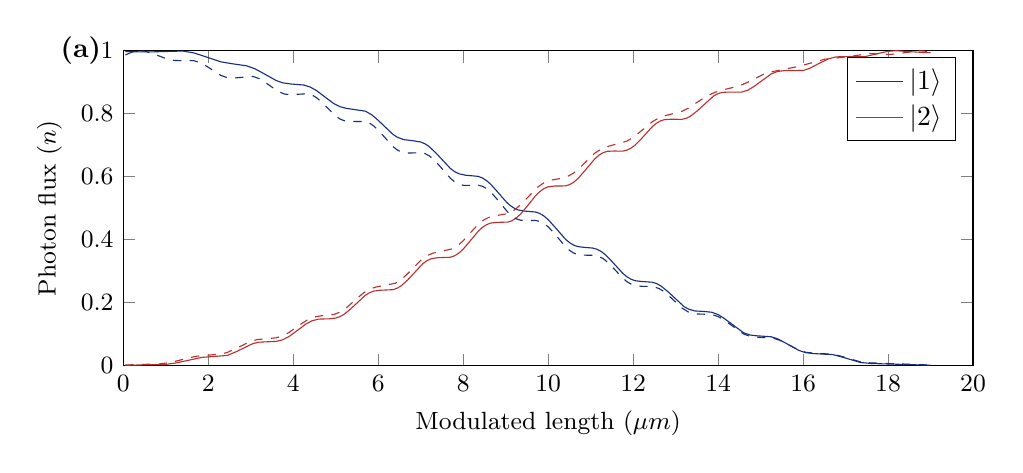
\begin{tikzpicture}

\begin{axis}[%
width=0.89\figW,
height=\figH,
at={(0\figW,0\figH)},
scale only axis,
xmin=0,
xmax=20,
ymin=0,
clip=false,
ymax=1,
xlabel = {Modulated length ($\mu m$)},
ylabel = {Photon flux ($n$)},
axis background/.style={fill=white}
]
\addplot [color=mode1]
  table[row sep=crcr]{%
0.0500000000000007	0.997209339000001\\
0.600000000000001	0.996082311999999\\
1.4	0.999022263000001\\
1.65	0.993382490999998\\
1.9	0.982718813000002\\
2.3	0.964655487000002\\
2.55	0.958933380000001\\
2.9	0.952184463000002\\
3.1	0.942576759000001\\
3.3	0.927887047999999\\
3.6	0.905261375999999\\
3.75	0.898179482\\
3.95	0.894331988000001\\
4.25	0.891038763000001\\
4.4	0.884646372999999\\
4.55	0.873285725999999\\
4.75	0.852737034\\
4.95	0.832707403000001\\
5.1	0.822307978000001\\
5.25	0.817025767000001\\
5.7	0.808020533000001\\
5.85	0.796413183999999\\
6	0.778965206999999\\
6.35	0.734063726999999\\
6.45	0.725368186000001\\
6.6	0.717762148999999\\
6.8	0.714571905\\
7	0.710239075000001\\
7.1	0.704527122000002\\
7.2	0.695582756\\
7.35	0.676607331\\
7.7	0.626013035\\
7.8	0.615969687\\
7.9	0.609305496000001\\
8.05	0.60488509\\
8.35	0.601126816000001\\
8.45	0.596091709\\
8.55	0.587603563000002\\
8.65	0.575691364000001\\
8.8	0.553178839000001\\
9	0.522013173000001\\
9.1	0.509348663000001\\
9.2	0.500006169999999\\
9.3	0.494200418999998\\
9.45	0.490807847999999\\
9.7	0.487941278000001\\
9.8	0.483361936000001\\
9.9	0.475333524\\
10	0.463777976999999\\
10.15	0.441435343999999\\
10.4	0.402711426\\
10.5	0.391020555000001\\
10.6	0.382831853999999\\
10.7	0.378095650999999\\
10.85	0.375642477\\
11.05	0.3735295\\
11.15	0.369619484000001\\
11.25	0.362489979999999\\
11.35	0.351964510999998\\
11.5	0.331161032000001\\
11.75	0.294155885999999\\
11.85	0.282716205\\
11.95	0.274574935\\
12.05	0.269782465999999\\
12.2	0.267346573000001\\
12.45	0.265035599000001\\
12.55	0.260834346999999\\
12.65	0.253599511000001\\
12.8	0.237392255\\
13.2	0.187501166000001\\
13.3	0.179857078000001\\
13.45	0.173855179\\
13.65	0.172357041000001\\
13.85	0.169724951999999\\
14	0.162292416\\
14.15	0.149391302000002\\
14.6	0.104563253999999\\
14.75	0.0974418640000003\\
14.9	0.09499396\\
15.25	0.0918480200000005\\
15.4	0.0853413819999993\\
15.6	0.0710626949999984\\
15.9	0.0485382899999998\\
16.05	0.0417482520000014\\
16.25	0.0384152650000011\\
16.7	0.0351825370000007\\
16.9	0.0281486870000016\\
17.35	0.0103134300000001\\
17.6	0.00701842200000158\\
19	0.00148695800000098\\
};
\addlegendentry{$\ket{1}$};
\addplot [color=mode2]
  table[row sep=crcr]{%
0.0500000000000007	0.00130598300000173\\
1	0.00400867200000121\\
1.25	0.00901523799999993\\
1.85	0.0263906570000003\\
2.45	0.032637703999999\\
2.65	0.0439684269999994\\
3.05	0.0701613660000007\\
3.2	0.0747393179999989\\
3.4	0.0759868879999992\\
3.6	0.0771289639999999\\
3.75	0.0821341589999989\\
3.9	0.0923892029999998\\
4.1	0.112325324\\
4.3	0.132503894999999\\
4.45	0.142997595000001\\
4.6	0.147944964000001\\
4.85	0.148831626\\
5	0.151200215999999\\
5.1	0.155822466\\
5.2	0.163467695000001\\
5.35	0.180056466\\
5.7	0.223845708999999\\
5.8	0.232024059\\
5.9	0.237034020999999\\
6.05	0.239504298\\
6.35	0.241410404\\
6.45	0.246267885000002\\
6.55	0.254644155000001\\
6.7	0.273296892000001\\
7.05	0.323916465\\
7.15	0.333628284\\
7.25	0.339698582\\
7.4	0.342845347000001\\
7.7	0.344257661\\
7.8	0.349064426999998\\
7.9	0.357711713\\
8	0.370116940999999\\
8.15	0.393714546999998\\
8.35	0.426048259000002\\
8.45	0.438825869999999\\
8.55	0.447869961999999\\
8.65	0.453002192\\
8.8	0.454976944999999\\
9.05	0.455989771999999\\
9.15	0.46050056\\
9.25	0.468945652999999\\
9.35	0.481335282\\
9.5	0.505348065\\
9.7	0.538942721000002\\
9.8	0.552489726000001\\
9.9	0.562260167000002\\
10	0.567977389999999\\
10.15	0.570399415000001\\
10.4	0.570791991\\
10.5	0.574658502999998\\
10.6	0.582342869000001\\
10.7	0.593951037\\
10.85	0.616955474000001\\
11.1	0.656995724000002\\
11.2	0.668787980000001\\
11.3	0.676677401999999\\
11.4	0.680713769\\
11.55	0.681555320000001\\
11.75	0.681265320000001\\
11.85	0.684219528\\
11.95	0.690689294999999\\
12.05	0.700869254000001\\
12.2	0.721617654999999\\
12.45	0.758751946\\
12.55	0.769948553999999\\
12.65	0.777569054000001\\
12.75	0.781569362999999\\
12.9	0.782457425\\
13.15	0.782154120000001\\
13.25	0.785593393999999\\
13.35	0.792298928000001\\
13.5	0.808085910999999\\
13.9	0.857002188999999\\
14	0.863983598000001\\
14.1	0.867771946000001\\
14.25	0.868751656000001\\
14.55	0.868512811999999\\
14.7	0.874832677000001\\
14.85	0.886968615000001\\
15.25	0.926425729999998\\
15.4	0.934265283999999\\
15.55	0.936641204000001\\
16	0.937225667\\
16.15	0.943829580999999\\
16.4	0.961348467000001\\
16.6	0.974242917000002\\
16.75	0.979810169\\
16.9	0.981439937000001\\
17.45	0.981089626999999\\
17.7	0.989015279\\
18	0.998277784999999\\
18.2	1\\
18.5	0.997101053000002\\
18.9	0.993978749\\
19	0.994044237000001\\
};
\addlegendentry{$\ket{2}$}
\addplot [color=mode1, dashed]
  table[row sep=crcr]{%
0.0500000000000007	0.986694052000001\\
0.199999999999999	0.995338852\\
0.350000000000001	0.999720845999999\\
0.5	0.998736347000001\\
0.649999999999999	0.992905961000002\\
1.1	0.970586748999999\\
1.25	0.968817562000002\\
1.65	0.968736516\\
1.8	0.96266893\\
1.95	0.951704654\\
2.3	0.921421076000001\\
2.45	0.914489442000001\\
2.6	0.913358597999999\\
3.05	0.918425266\\
3.2	0.911459430000001\\
3.35	0.898777691999999\\
3.65	0.870176603000001\\
3.8	0.862215405000001\\
3.95	0.860582315999999\\
4.35	0.863610502\\
4.45	0.859005038999999\\
4.55	0.850809978000001\\
4.7	0.832837961999999\\
5	0.792670651000002\\
5.1	0.783428644000001\\
5.2	0.777721363000001\\
5.35	0.775212203999999\\
5.7	0.775125292999999\\
5.8	0.769786952\\
5.9	0.760574705\\
6.05	0.740514132000001\\
6.35	0.695389793\\
6.45	0.684781181000002\\
6.55	0.678039108\\
6.65	0.675047397\\
6.8	0.675445301\\
7	0.676491379000002\\
7.1	0.67344808\\
7.2	0.666571595000001\\
7.3	0.655718989\\
7.45	0.633696021999999\\
7.7	0.594953963000002\\
7.8	0.583650304999999\\
7.9	0.576265646\\
8	0.572737298\\
8.15	0.572549955\\
8.35	0.573068835000001\\
8.45	0.56976654\\
8.55	0.562569932999999\\
8.65	0.551291265\\
8.8	0.528351226000002\\
9.05	0.487278348\\
9.15	0.474875100999999\\
9.25	0.46642327\\
9.35	0.461965199000002\\
9.5	0.460841005999999\\
9.7	0.46120307\\
9.8	0.458263487\\
9.9	0.451640051999998\\
10	0.441052800000001\\
10.15	0.419146350999998\\
10.4	0.378993314999999\\
10.5	0.366502645000001\\
10.6	0.357714438999999\\
10.7	0.352761213000001\\
10.85	0.350919177000002\\
11.1	0.350448699000001\\
11.2	0.346637943000001\\
11.3	0.339333867000001\\
11.4	0.328559826999999\\
11.55	0.307720994\\
11.75	0.278821315999998\\
11.85	0.267281336\\
11.95	0.259008083000001\\
12.05	0.254180084000001\\
12.2	0.252071075\\
12.45	0.251483852\\
12.6	0.245501526999998\\
12.7	0.237664842000001\\
12.85	0.220868841000001\\
13.15	0.183089106000001\\
13.3	0.170449332\\
13.45	0.164485076999998\\
13.65	0.163598780000001\\
13.85	0.162269086999999\\
14	0.15603861\\
14.15	0.144254965999998\\
14.6	0.100622414\\
14.75	0.0933171520000009\\
14.9	0.0907820719999997\\
15.3	0.0875060310000002\\
15.45	0.0807486439999998\\
15.65	0.0669081769999984\\
15.9	0.049559704\\
16.05	0.0429908810000015\\
16.25	0.0396613419999987\\
16.7	0.0365461459999992\\
16.9	0.0297755170000009\\
17.35	0.0121282299999983\\
17.55	0.00921560100000107\\
19	0.00205285599999883\\
};
%\addlegendentry{$\ket{1}$ TD};
\addplot [color=mode2, dashed]
  table[row sep=crcr]{%
0.0500000000000007	0.00221802900000156\\
0.850000000000001	0.00582627400000035\\
1.1	0.0097343770000009\\
1.4	0.0198939749999987\\
1.7	0.029623492999999\\
1.95	0.0329643090000005\\
2.3	0.03675286\\
2.45	0.0422475300000009\\
2.65	0.0544176450000009\\
3	0.0775024649999985\\
3.15	0.0828504069999987\\
3.35	0.0854133419999989\\
3.6	0.0886016000000005\\
3.75	0.0947910790000002\\
3.9	0.10543096\\
4.15	0.129462504999999\\
4.35	0.146831486\\
4.5	0.154842831\\
4.65	0.158284257999998\\
4.95	0.162379112\\
5.1	0.170050675999999\\
5.25	0.183598153999998\\
5.45	0.207654961999999\\
5.65	0.230807343999999\\
5.8	0.243064097000001\\
5.95	0.249822298000002\\
6.4	0.261662499\\
6.5	0.269430125\\
6.65	0.286602654999999\\
7.05	0.340965801999999\\
7.15	0.349817611999999\\
7.3	0.357632011\\
7.75	0.371192294\\
7.85	0.379247058000001\\
8	0.396694839999999\\
8.25	0.433824799\\
8.4	0.453948307000001\\
8.5	0.463998901\\
8.6	0.470805353999999\\
8.75	0.475859165999999\\
9.05	0.482985608\\
9.15	0.489356490999999\\
9.25	0.498796601999999\\
9.4	0.517851310000001\\
9.75	0.566569400999999\\
9.9	0.580676912000001\\
10.05	0.588715038\\
10.3	0.594643509000001\\
10.45	0.600281448\\
10.6	0.61165759\\
10.75	0.629107645000001\\
11.1	0.675062894\\
11.25	0.688151403999999\\
11.4	0.695901053\\
11.85	0.712871225000001\\
12	0.724777358000001\\
12.2	0.746461385\\
12.45	0.774416689999999\\
12.6	0.786430815999999\\
12.75	0.793687932000001\\
13.15	0.807606872000001\\
13.3	0.817792232999999\\
13.6	0.844549375\\
13.8	0.860627362999999\\
14	0.871852792999999\\
14.25	0.880085314999999\\
14.5	0.888553403\\
14.7	0.900148941000001\\
15.1	0.927127182\\
15.3	0.934342208\\
15.9	0.950310096999999\\
16.5	0.972822297\\
16.75	0.976590496\\
17.1	0.981624049000001\\
17.55	0.991271328\\
17.8	0.98955943\\
18.05	0.988140959999999\\
18.3	0.991819562\\
18.7	0.999900176000001\\
18.85	0.999009899000001\\
19	0.99430156\\
};
\node at (-1, 1) {\textbf{(a)}};
%\addlegendentry{$\ket{2}$ TD};
\end{axis}
\end{tikzpicture}%
		\phantomsubcaption%
		\label{sfig:coherence}%
	\end{subfigure}
	\setlength{\figH}{0.3\textwidth}
	\setlength{\figW}{0.4\textwidth}
	\begin{subfigure}{0.5\textwidth}
		\centering
		% This file was created by matlab2tikz.
%
%The latest updates can be retrieved from
%  http://www.mathworks.com/matlabcentral/fileexchange/22022-matlab2tikz-matlab2tikz
%where you can also make suggestions and rate matlab2tikz.
%
\begin{tikzpicture}

\begin{axis}[%
width=\figW,
height=0.5\figH,
at={(0\figW,0\figH)},
scale only axis,
point meta min=-4.99371933183411,
point meta max=4.99371933183411,
title = {},
axis on top,
xmin=0,
xmax=23,
clip=false,
xlabel={$\text{x (}\mu\text{m)}$},
ymin=-2.5,
ymax=2.5,
ylabel={$\text{y (}\mu\text{m)}$},
axis background/.style={fill=white},
colormap={mymap}{[1pt] rgb(0pt)=(0,0,1); rgb(31pt)=(1,1,1); rgb(32pt)=(1,1,1); rgb(63pt)=(1,0,0)}
]
\addplot [forget plot] graphics [xmin=0, xmax=23, ymin=-2.5, ymax=2.5] {graphs/fdfd/reciprocal/mode1-1.png};
\draw (0,0.55) -- (23,0.55);
\draw (0,-0.55) -- (23,-0.55);
\node at (2,1.8) {$\ket{1}$};
\node at (-1,3.3) {\textbf{(b)}};
\end{axis}
\end{tikzpicture}%
		\phantomsubcaption%
		\label{sfig:mode1}%
	\end{subfigure}%
	\begin{subfigure}{0.5\textwidth}
		\centering
		% This file was created by matlab2tikz.
%
%The latest updates can be retrieved from
%  http://www.mathworks.com/matlabcentral/fileexchange/22022-matlab2tikz-matlab2tikz
%where you can also make suggestions and rate matlab2tikz.
%
\begin{tikzpicture}

\begin{axis}[%
width=\figW,
height=0.5\figH,
at={(0\figW,0\figH)},
scale only axis,
point meta min=-4.99371933183411,
point meta max=4.99371933183411,
%title = {$\ket{2}$},
axis on top,
xmin=0,
clip=false,
xmax=23,
xlabel style={font=\color{white!15!black}},
xlabel={$\text{x (}\mu\text{m)}$},
ymin=-2.5,
ymax=2.5,
ylabel style={font=\color{white!15!black}},
axis background/.style={fill=white},
colormap={mymap}{[1pt] rgb(0pt)=(0,0,1); rgb(31pt)=(1,1,1); rgb(32pt)=(1,1,1); rgb(63pt)=(1,0,0)},
colorbar,
colorbar style={width=.02\linewidth, at={(1.05,0.25\figH)}, anchor=east}
]
\addplot [forget plot] graphics [xmin=0, xmax=23, ymin=-2.5, ymax=2.5] {graphs/fdfd/reciprocal/mode2-1.png};
\draw (0,0.55) -- (23,0.55);
\draw (0,-0.55) -- (23,-0.55);
\node at (2,1.8) {$\ket{2}$};
\node at (-1,3.3) {\textbf{(c)}};
\end{axis}
\end{tikzpicture}%
		\phantomsubcaption%
		\label{sfig:mode2}%
	\end{subfigure}
	\caption[Comparison of mode transition for FDTD and FDFD]{\textbf{(a)} Amplitude of both modes $\ket{1}$ and $\ket{2}$ for the time and frequency domain simulations, with the time domain in dashed lines. \textbf{(b)}Mode evolution of $\ket{1}$ as it propagates through the waveguide, and likewise for \textbf{(c)} $\ket{2}$. Note how $\ket{1}$ completely vanishes after reaching the coherence length.}
	\label{fig:coherencelength}
\end{figure} 


\subsection{Direct validation through coupled-mode theory}

The finite difference method simulates modes over any number of given sidebands. However, the implementation of the time domain method provided here is incapable of extracting these sidebands. Thus, to independently verify the frequency domain implementation, a simulation of a dynamically modulated waveguide over several sidebands is performed and compared to coupled-mode theory. Since the previously shown coupled mode-theory assumes only transitions between two modes (Equation \ref{eqn:theorymode}), a differential equation that describes transitions between $n$ modes is derived in Appendix \ref{app:cmt}. This allows for the comparison of the MF-FDFD implementation against a semi-analytic result.

The simulation considers a slab waveguide of relative permittivity $\epsilon= 4$ surrounded by vacuum in a region $10 \times 4  \mskip3mu \mu m$ discretised to $\Delta = 0.04 \mskip3mu  \mu m$. The waveguide is $10  \mskip3mu \mu m$ long and $0.75  \mskip3mu \mu m$ wide, which leads to a choice of an even mode of $\omega_1 = 0.667  \mskip3mu (2\pi c/a)$ at $k_1 = 0.841 \mskip3mu  (2\pi /a)$ and an odd mode at $\omega_2 = 0.645 \mskip3mu  (2\pi c/a)$ and $k_2 = 1.097 \mskip3mu  (2\pi /a)$. A permittivity modulation of $0.1 \epsilon_0 \cos(\Omega t)$ is applied between $1.5$ and $9 \mskip3mu  \mu m$, where the top and bottom halves of the waveguide are modulated with a $\pi$ phase difference to maximise coupling. This weak choice of modulation is insufficient to transition a mode, however coupled mode theory becomes exact in the limit of small modulations. Thus, it is perfectly suited to analysing the response of FDFD. The simulation is truncated to 5 frequency sidebands for $\omega_n = \omega_1 + n \Omega$ where $n \in [-4,4]$, and a continuous wave input of the first mode is excited at location $1 \mskip3mu  \mu m$ using the standard solver, whose power is normalised to $1  \mskip3mu W \mu m^{-1}$. For each frequency sideband the amplitude of the mode is extracted and compared to the semi-analytic results provided by the coupled-mode theory equation \ref{eqn:cmttheory}.

The maximum $|E_z|^2$ field at each sideband $\omega_n$ is first extracted and shown in figure \ref{fig:sideamp}. At the initial band $\omega_1$, the field amplitude is normalised to unity. The fields exponentially decrease with $|n|$. However, the higher sidebands decrease at a slower rate than that of the negative sidebands. Importantly, this means that the impact of reducing the sideband count in the simulation is minimal for a weak modulation. Since the final fields are the sum of each field component at all the sidebands calculated, any missing sidebands will lead to a slight inaccuracy in the final result. Here, the combined second sideband frequencies have a maximum amplitude of less than $0.0001 \% $ of the initial mode.

\begin{figure}[t]
	\centering
	\setlength{\figH}{\textwidth}
	\setlength{\figW}{\textwidth}
	% This file was created by matlab2tikz.
%
%The latest updates can be retrieved from
%  http://www.mathworks.com/matlabcentral/fileexchange/22022-matlab2tikz-matlab2tikz
%where you can also make suggestions and rate matlab2tikz.
%
\definecolor{mycolor1}{rgb}{0.00000,0.44700,0.74100}%
%
\begin{tikzpicture}

\begin{axis}[%
width=0.8\figW,
height=0.25\figH,
at={(0\figW,0\figH)},
scale only axis,
xmin=-3,
xmax=3,
xtick={-3,-2,-1,0,1,2,3},
yminorticks=false,
xlabel={Sideband (n)},
ymode=log,
ymin=0.00000001,
ymax=10,
grid=both,
ylabel = {Maximum $|E_z (\omega_n)|^2$},
%ylabel={$\text{Maximum $|$E}_\text{z}\text{(}\omega{}_\text{n}\text{)$|$}$},
axis background/.style={fill=white}
]
\addplot[only marks, mark=*, mark options={}, mark size=3.000pt, draw=black, fill=mycolor1] table[row sep=crcr]{%
x	y\\
-3	0.000000058939162\\
-2	0.000049831160601\\
-1	0.003480773455234\\
0	1.010334172885610\\
1	0.011021244259482\\
2	0.000107038587645\\
3	0.000002341788501\\
};
\end{axis}
\end{tikzpicture}%
	\caption[Maximum $|E_z(\omega_n)|$ field amplitude at each sideband $n$.]{The maximum field amplitude calculated for each sideband $n$ on a log scale. The field intensity decreases exponentially with $n$. Note that the amplitude of the sidebands is not symmetric about $n=0$.}
	\label{fig:sideamp}
\end{figure}

The results of the simulation for the modal profile and corresponding amplitudes in each mode are shown in Figure \ref{fig:weakMod}. There is an excellent agreement between CMT and FDFD in Figure \ref{sfig:cmtcompare}. However, FDFD shows minor oscillations along the length of the waveguide that CMT can not predict, identical to the oscillations in previous simulations with only temporal modulations. By performing a standard Fourier transform on the modal amplitude at frequency sideband $\omega_1+\Omega$, the minor oscillation is found to be at a period of $T=0.075  \mskip3mu \mu m$. This period corresponds exactly to the generation of backward propagating modes, $0.075  \mskip3mu \mu m = 1/(k_1+k_2)$.


\begin{figure}[h!]
	\centering
	\setlength{\figH}{1\linewidth}
	\setlength{\figW}{1\textwidth}
	\begin{subfigure}[t]{0.5\textwidth}
		% This file was created by matlab2tikz.
%
%The latest updates can be retrieved from
%  http://www.mathworks.com/matlabcentral/fileexchange/22022-matlab2tikz-matlab2tikz
%where you can also make suggestions and rate matlab2tikz.
%
\pgfplotsset{weakMod/.style={
	width=0.32\figW,
	height=0.15\figH,
	scale only axis,
	axis on top,
	xmin=0,
	xmax=10,
	ymin=-2.5,
	ymax=2.5,
	%xlabel style={font=\color{white!15!black}},
	%ylabel style={font=\color{white!15!black}},
	axis background/.style={fill=white},
	colormap={mymap}{[1pt] rgb(0pt)=(0,0,1); rgb(31pt)=(1,1,1); rgb(32pt)=(1,1,1); rgb(63pt)=(1,0,0)},
	colorbar,
	colorbar style={width=.03\linewidth, at={(1.08,0.075\figH)}, anchor=east}
	}
}

\begin{tikzpicture}

\begin{axis}[%
weakMod,
at={(0\figW,0.92\figH)},
point meta min=-0.153883565276573,
point meta max=0.153883565276573,
xticklabels={,,},
colorbar style={title = $V / \mu m$, width=.03\linewidth, at={(1.08,0.075\figH)}, anchor=east}
]
\addplot [forget plot] graphics [xmin=0, xmax=10, ymin=-2.5, ymax=2.5] {graphs/weakmod/nameoffile2-1.png};
\draw (0,-0.5) -- (10,-0.5);
\draw (0,0.5) -- (10,0.5);
\node at (5,1.8) {$\omega_1+2\Omega$};
\end{axis}

\begin{axis}[%
weakMod,
at={(0\figW,0.69\figH)},
point meta min=-1.37640682053953,
point meta max=1.37640682053953,
xticklabels={,,}
]
\addplot [forget plot] graphics [xmin=0, xmax=10, ymin=-2.5, ymax=2.5] {graphs/weakmod/nameoffile2-2.png};
\draw (0,-0.5) -- (10,-0.5);
\draw (0,0.5) -- (10,0.5);
\node at (5,1.8) {$\omega_1+\Omega$};
\end{axis}

\begin{axis}[%
weakMod,
at={(0\figW,0.46\figH)},
point meta min=-24.7127053691998,
point meta max=24.7127053691998,
xticklabels={,,},
ylabel={$\text{y (}\mu\text{m)}$}
]
\addplot [forget plot] graphics [xmin=0, xmax=10, ymin=-2.5, ymax=2.5] {graphs/weakmod/nameoffile2-3.png};
\draw (0,-0.5) -- (10,-0.5);
\draw (0,0.5) -- (10,0.5);
\node at (5,1.8) {$\omega_1$};
\end{axis}

\begin{axis}[%
weakMod,
at={(0\figW,0.23\figH)},
point meta min=-2.69144358712869,
point meta max=2.69144358712869,
xticklabels={,,}
]
\addplot [forget plot] graphics [xmin=0, xmax=10, ymin=-2.5, ymax=2.5] {graphs/weakmod/nameoffile2-4.png};
\draw (0,-0.5) -- (10,-0.5);
\draw (0,0.5) -- (10,0.5);
\node at (5,1.8) {$\omega_1-\Omega$};
\end{axis}

\begin{axis}[%
weakMod,
at={(0\figW,0\figH)},
point meta min=-0.251011435268562,
point meta max=0.251011435268562,
%xlabel style={font=\color{white!15!black}},
xlabel={$\text{x (}\mu\text{m)}$}
]
\addplot [forget plot] graphics [xmin=0, xmax=10, ymin=-2.5, ymax=2.5] {graphs/weakmod/nameoffile2-5.png};
\draw (0,-0.5) -- (10,-0.5);
\draw (0,0.5) -- (10,0.5);
\node at (5,1.8) {$\omega_1-2\Omega$};
\end{axis}
\node at (-1,16) {\textbf{(a)}};

\end{tikzpicture}%
		\phantomsubcaption
		\label{sfig:weakmod}
	\end{subfigure}%
	\begin{subfigure}[t]{0.5\textwidth}
		% This file was created by matlab2tikz.
%
%The latest updates can be retrieved from
%  http://www.mathworks.com/matlabcentral/fileexchange/22022-matlab2tikz-matlab2tikz
%where you can also make suggestions and rate matlab2tikz.
%
\definecolor{mycolor1}{rgb}{0.00000,0.44700,0.74100}%
\definecolor{mycolor2}{rgb}{0.85000,0.32500,0.09800}%
%
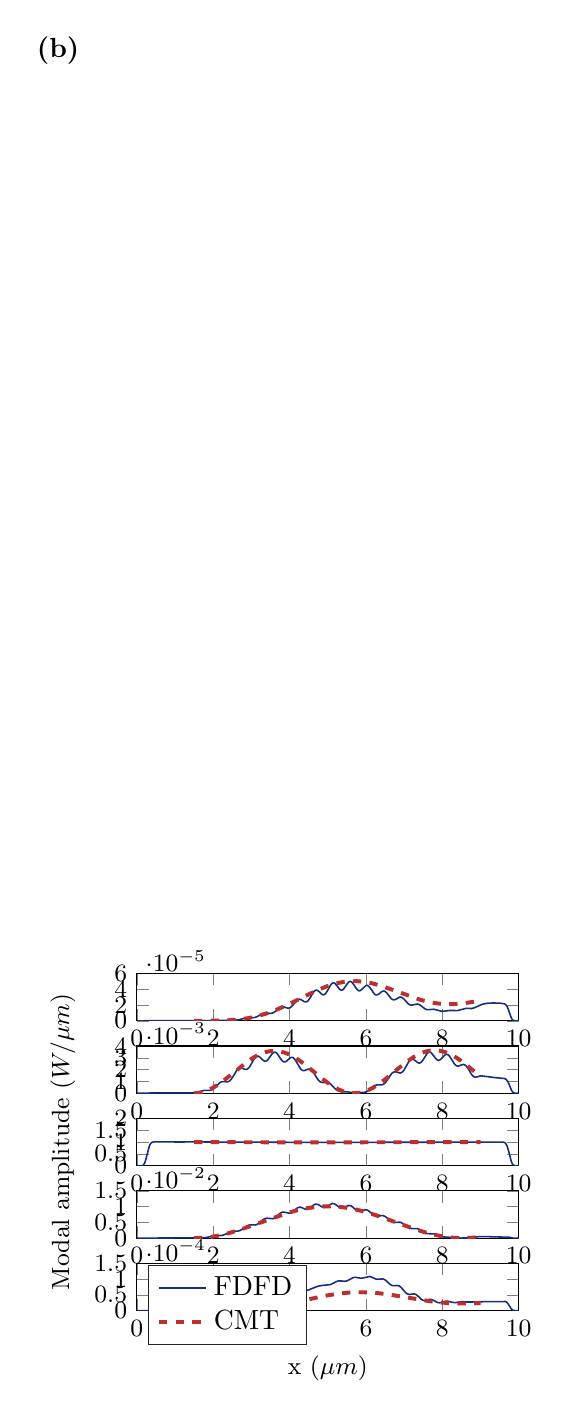
\begin{tikzpicture}

\begin{axis}[%
width=0.4\figW,
height=0.15\figH,
at={(0\figW,0.92\figH)},
scale only axis,
xmin=0,
xmax=10,
ymin=0,
ymax=0.00006,
axis background/.style={fill=white}
]
\addplot [color=mode1, forget plot, line width = 0.2mm]
  table[row sep=crcr]{%
0	5.43387557172537e-12\\
2.33082706766917	4.15554692878573e-07\\
2.58145363408521	8.04269815191105e-07\\
2.65664160401002	1.13458524886312e-06\\
2.78195488721805	2.75443581720936e-06\\
2.88220551378446	3.82980313062831e-06\\
2.98245614035088	3.84802184072441e-06\\
3.08270676691729	4.09176513294085e-06\\
3.15789473684211	5.51922256164517e-06\\
3.30827067669173	9.65933932128848e-06\\
3.35839598997494	1.01329342037104e-05\\
3.43358395989975	9.7503546498956e-06\\
3.50877192982456	9.34698401167111e-06\\
3.55889724310777	9.92427050050537e-06\\
3.60902255639098	1.14338577574813e-05\\
3.7593984962406	1.74508023960129e-05\\
3.80952380952381	1.79598131815339e-05\\
3.85964912280702	1.74420039549261e-05\\
3.95989974937343	1.5946668758815e-05\\
4.01002506265664	1.65844142241411e-05\\
4.06015037593985	1.86403991353501e-05\\
4.21052631578947	2.6945067729045e-05\\
4.26065162907268	2.74805266418099e-05\\
4.31077694235589	2.65258951159808e-05\\
4.3859649122807	2.42953819480363e-05\\
4.43609022556391	2.40423073325502e-05\\
4.46115288220551	2.46232051370754e-05\\
4.48621553884712	2.57137243551142e-05\\
4.53634085213033	2.91782066437207e-05\\
4.61152882205514	3.54291152433461e-05\\
4.63659147869674	3.70793879191922e-05\\
4.66165413533835	3.82557620248747e-05\\
4.68671679197995	3.88727722544502e-05\\
4.71177944862155	3.89096848198989e-05\\
4.76190476190476	3.74991024223448e-05\\
4.83709273182957	3.40173678701206e-05\\
4.86215538847118	3.32774330153995e-05\\
4.88721804511278	3.30322850192744e-05\\
4.91228070175439	3.33779784380539e-05\\
4.93734335839599	3.43402589280117e-05\\
4.9874686716792	3.78494222292858e-05\\
5.06265664160401	4.45703653060292e-05\\
5.08771929824561	4.63538804211794e-05\\
5.11278195488722	4.75991495889616e-05\\
5.13784461152882	4.81981292086431e-05\\
5.16290726817043	4.81164536676459e-05\\
5.18796992481203	4.73979463677665e-05\\
5.23809523809524	4.45784691347484e-05\\
5.28822055137845	4.12604051298615e-05\\
5.31328320802005	3.99650311706523e-05\\
5.33834586466165	3.91564508568365e-05\\
5.36340852130326	3.89468195542975e-05\\
5.38847117794486	3.93737780388648e-05\\
5.41353383458647	4.03960161818873e-05\\
5.46365914786968	4.37060878120121e-05\\
5.51378446115288	4.73716227489263e-05\\
5.53884711779449	4.8792712444623e-05\\
5.56390977443609	4.96983863111922e-05\\
5.58897243107769	4.99787618970515e-05\\
5.6140350877193	4.95976774299578e-05\\
5.6390977443609	4.85966020402628e-05\\
5.68922305764411	4.52463159970051e-05\\
5.73934837092732	4.13970089834237e-05\\
5.78947368421053	3.86834879577691e-05\\
5.81453634085213	3.81146134031951e-05\\
5.83959899749373	3.81368506499058e-05\\
5.88972431077694	3.97151141680041e-05\\
5.98997493734336	4.44888289692358e-05\\
6.01503759398496	4.4936094301562e-05\\
6.04010025062657	4.48320064965202e-05\\
6.06516290726817	4.41567615894201e-05\\
6.11528822055138	4.13568523640606e-05\\
6.2155388471178	3.43621038911834e-05\\
6.2406015037594	3.33363328692826e-05\\
6.265664160401	3.28240666522817e-05\\
6.29072681704261	3.28347284828112e-05\\
6.34085213032582	3.41444278788572e-05\\
6.41604010025063	3.71238134793117e-05\\
6.46616541353383	3.78701941219362e-05\\
6.49122807017544	3.75468914661781e-05\\
6.54135338345865	3.55134953480274e-05\\
6.66666666666667	2.78181785517972e-05\\
6.71679197994987	2.65938751233818e-05\\
6.76691729323308	2.70466771130629e-05\\
6.8922305764411	3.02023964877662e-05\\
6.94235588972431	2.97020206154741e-05\\
6.99248120300752	2.77162762500893e-05\\
7.11779448621554	2.1098852439394e-05\\
7.16791979949875	1.99746805016332e-05\\
7.21804511278195	2.00616584091762e-05\\
7.34335839598998	2.13945187006459e-05\\
7.39348370927318	2.06580379806809e-05\\
7.44360902255639	1.90186907857992e-05\\
7.54385964912281	1.51863402155783e-05\\
7.59398496240602	1.42171264769786e-05\\
7.64411027568922	1.41290804887007e-05\\
7.76942355889724	1.46969967094179e-05\\
7.84461152882206	1.39259300944161e-05\\
7.96992481203008	1.2162203580246e-05\\
8.04511278195489	1.22613284752049e-05\\
8.19548872180451	1.31556729527915e-05\\
8.39598997493734	1.29831159423333e-05\\
8.62155388471178	1.58658634550335e-05\\
8.7719298245614	1.55996883623999e-05\\
8.84711779448622	1.67615595980664e-05\\
9.04761904761905	2.10964253533064e-05\\
9.17293233082707	2.22552359279149e-05\\
9.32330827067669	2.26945466739181e-05\\
9.52380952380952	2.23158718224425e-05\\
9.62406015037594	2.15477535139286e-05\\
9.64912280701754	2.08446471621215e-05\\
9.67418546365915	1.95987671691711e-05\\
9.69924812030075	1.76196276182594e-05\\
9.72431077694236	1.48288148107412e-05\\
9.79949874686717	4.43934645133481e-06\\
9.82456140350877	2.07846284006052e-06\\
9.84962406015038	7.5191475090719e-07\\
9.89974937343358	3.57357858860041e-08\\
10	3.59374752179065e-11\\
};
\addplot [color=mode2, dashed, forget plot, line width = 0.5mm]
  table[row sep=crcr]{%
1.5	0\\
2.331	4.55758724982047e-07\\
2.655	1.59956065992617e-06\\
2.923	3.4474900711956e-06\\
3.168	6.04500525369644e-06\\
3.407	9.49516199177936e-06\\
3.654	1.39891369101974e-05\\
3.931	1.99746349487384e-05\\
4.352	3.01312148938138e-05\\
4.742	3.92109647950889e-05\\
4.985	4.39479584990465e-05\\
5.194	4.71192896878136e-05\\
5.388	4.91524537000743e-05\\
5.574	5.01925575964179e-05\\
5.759	5.0313296824811e-05\\
5.948	4.9516196257926e-05\\
6.147	4.77524459796541e-05\\
6.368	4.4856263265558e-05\\
6.64	4.03262877739508e-05\\
7.442	2.63712804393634e-05\\
7.676	2.35983383820582e-05\\
7.894	2.19240859902214e-05\\
8.11	2.11825016283029e-05\\
8.335	2.13363968892821e-05\\
8.586	2.24494528513475e-05\\
8.916	2.49038214494846e-05\\
9.001	2.56222738137524e-05\\
};
\end{axis}

\begin{axis}[%
width=0.4\figW,
height=0.15\figH,
at={(0\figW,0.69\figH)},
scale only axis,
xmin=0,
xmax=10,
ymin=0,
ymax=0.004,
axis background/.style={fill=white}
]
\addplot [color=mode1, forget plot, line width = 0.2mm]
  table[row sep=crcr]{%
0	4.54703830143899e-09\\
0.275689223057643	1.51941339936457e-05\\
0.451127819548873	2.52401768339183e-05\\
1.45363408521303	3.97304625625594e-05\\
1.57894736842105	6.51259869020038e-05\\
1.67919799498747	0.000175895551990379\\
1.75438596491228	0.000238974537602132\\
1.80451127819549	0.000246791504064703\\
1.92982456140351	0.000239343214227361\\
1.97994987468672	0.000305673061468781\\
2.03007518796993	0.000434091444263984\\
2.18045112781955	0.000912147145111675\\
2.23057644110276	0.000983880445240004\\
2.28070175438597	0.000991559270044462\\
2.35588972431078	0.000964418411161461\\
2.38095238095238	0.000972484533821927\\
2.40601503759398	0.000999816229947825\\
2.43107769423559	0.00105053818120737\\
2.45614035087719	0.00112635861105836\\
2.4812030075188	0.00122625651255603\\
2.53132832080201	0.00148084340935029\\
2.60651629072682	0.00188509814085691\\
2.63157894736842	0.00199144331246615\\
2.65664160401002	0.00207218449949842\\
2.68170426065163	0.0021240587850464\\
2.70676691729323	0.00214693945004818\\
2.73182957393484	0.00214393345262565\\
2.78195488721805	0.00208688515637867\\
2.83208020050125	0.00202400707654427\\
2.85714285714286	0.00201496718057115\\
2.88220551378446	0.00203150059589774\\
2.90726817042606	0.00207831371054645\\
2.93233082706767	0.00215671027678077\\
2.95739348370927	0.0022643620082814\\
3.00751879699248	0.0025414201334204\\
3.05764411027569	0.00283435053856174\\
3.08270676691729	0.00295887002931572\\
3.1077694235589	0.00305573849594509\\
3.1328320802005	0.00311834405742673\\
3.15789473684211	0.00314358226193256\\
3.18295739348371	0.00313224450067473\\
3.20802005012531	0.00308897408162245\\
3.25814536340852	0.00294122463663626\\
3.30827067669173	0.00278758958814684\\
3.33333333333333	0.00273712601422815\\
3.35839598997494	0.00271596254521178\\
3.38345864661654	0.00272886128914784\\
3.40852130325815	0.0027766139994565\\
3.43358395989975	0.00285592725976613\\
3.48370927318296	0.00307810386792262\\
3.53383458646617	0.0033101077573594\\
3.55889724310777	0.00339963070497085\\
3.58395989974937	0.00345805104941022\\
3.60902255639098	0.003478974154973\\
3.63408521303258	0.00345988347483761\\
3.65914786967419	0.0034024206088823\\
3.68421052631579	0.00331220269436017\\
3.734335839599	0.00307172899026398\\
3.78446115288221	0.00283081470250757\\
3.80952380952381	0.00273905339945557\\
3.83458646616541	0.00267770592568972\\
3.85964912280702	0.00265093954249096\\
3.88471177944862	0.00265888376477719\\
3.90977443609023	0.00269764826026275\\
3.95989974937343	0.00283515653665312\\
4.01002506265664	0.00297856489579118\\
4.03508771929825	0.00302381999546419\\
4.06015037593985	0.00303925153206919\\
4.08521303258145	0.00301948476103142\\
4.11027568922306	0.00296290260591903\\
4.13533834586466	0.00287177955390128\\
4.16040100250627	0.0027519817970667\\
4.28571428571429	0.00207037848208813\\
4.31077694235589	0.00198659640263799\\
4.33583959899749	0.00193412267554471\\
4.3609022556391	0.0019123927148641\\
4.3859649122807	0.0019174008621512\\
4.43609022556391	0.00197788032427049\\
4.48621553884712	0.0020417130894117\\
4.51127819548872	0.00205130671514731\\
4.53634085213033	0.00203658351918001\\
4.56140350877193	0.00199381962574208\\
4.58646616541354	0.00192244234541938\\
4.61152882205514	0.00182500414846665\\
4.66165413533835	0.00157523886027811\\
4.71177944862155	0.00130652783535545\\
4.73684210526316	0.00118622064949392\\
4.76190476190476	0.00108437914613191\\
4.78696741854637	0.00100516848711329\\
4.81203007518797	0.000950135940101404\\
4.83709273182957	0.000918158812790892\\
4.88721804511278	0.000907303483790756\\
4.96240601503759	0.000929034010150431\\
5.0125313283208	0.000896952321081557\\
5.06265664160401	0.00079894934214586\\
5.11278195488722	0.000645880618932893\\
5.18796992481203	0.000390709941234135\\
5.23809523809524	0.000258840265729532\\
5.28822055137845	0.000180937135505488\\
5.33834586466165	0.000151603943791656\\
5.51378446115288	0.000113800961187849\\
5.6390977443609	6.21770847697434e-05\\
5.78947368421053	5.24380355457765e-05\\
5.96491228070176	7.84555890245286e-05\\
6.01503759398496	0.000130318856328415\\
6.06516290726817	0.000225790194559039\\
6.14035087719298	0.000427707834578683\\
6.19047619047619	0.000563921729051842\\
6.2406015037594	0.000662944169352642\\
6.29072681704261	0.000708167027404727\\
6.36591478696742	0.000705086318014025\\
6.41604010025063	0.000713226201307648\\
6.44110275689223	0.000737790514449443\\
6.46616541353383	0.000781916048628872\\
6.49122807017544	0.000847750307238826\\
6.51629072681704	0.000935132553516738\\
6.56641604010025	0.00116195270580377\\
6.64160401002506	0.00153687222175236\\
6.66666666666667	0.00164039371462898\\
6.69172932330827	0.00172220950571145\\
6.71679197994987	0.00177864525240246\\
6.74185463659148	0.00180877963818382\\
6.76691729323308	0.00181464955592503\\
6.81704260651629	0.0017754218481727\\
6.8671679197995	0.00172355971527338\\
6.8922305764411	0.0017159814746055\\
6.91729323308271	0.00173128501731767\\
6.94235588972431	0.00177470332045004\\
6.96741854636591	0.00184841304357697\\
6.99248120300752	0.00195119297812596\\
7.04260651629073	0.00222268886600574\\
7.09273182957394	0.00252206211549932\\
7.11779448621554	0.00265552955625914\\
7.14285714285714	0.00276499269115327\\
7.16791979949875	0.00284319688935497\\
7.19298245614035	0.00288606816143044\\
7.21804511278195	0.00289322297041927\\
7.24310776942356	0.00286807274911283\\
7.29323308270677	0.00275116515563845\\
7.34335839598998	0.0026171503447916\\
7.36842105263158	0.0025723605928647\\
7.39348370927318	0.00255501862322838\\
7.41854636591479	0.0025709690230169\\
7.44360902255639	0.0026222874078492\\
7.468671679198	0.00270699266448382\\
7.4937343358396	0.00281922232698761\\
7.59398496240602	0.00333386858474327\\
7.61904761904762	0.00342005360670861\\
7.64411027568922	0.00347034676450342\\
7.66917293233083	0.00348072246716669\\
7.69423558897243	0.00345127595672778\\
7.71929824561404	0.00338621759606461\\
7.76942355889724	0.0031835055709788\\
7.81954887218045	0.00296169654041378\\
7.84461152882206	0.00287370758437611\\
7.86967418546366	0.00281382081844761\\
7.89473684210526	0.00278770924458982\\
7.91979949874687	0.00279708711230953\\
7.94486215538847	0.00283954727636626\\
7.99498746867168	0.00299568097608116\\
8.04511278195489	0.00317557211279151\\
8.07017543859649	0.00324493174914409\\
8.09523809523809	0.00328701658403574\\
8.1203007518797	0.00329504635814359\\
8.1453634085213	0.00326587523138322\\
8.17042606516291	0.00320029460965898\\
8.19548872180451	0.00310289184400503\\
8.24561403508772	0.00284620682331926\\
8.29573934837093	0.00257900767152819\\
8.32080200501253	0.00246800328467955\\
8.34586466165413	0.00238264575786573\\
8.37092731829574	0.00232704219100377\\
8.39598997493734	0.00230168183730228\\
8.42105263157895	0.0023034547439984\\
8.47117794486216	0.0023608828545445\\
8.52130325814536	0.00242677020097304\\
8.54636591478697	0.00243847452169277\\
8.57142857142857	0.00242582230027999\\
8.59649122807017	0.00238452321434934\\
8.62155388471178	0.00231358718829178\\
8.64661654135338	0.00221539591423436\\
8.69674185463659	0.0019614030422801\\
8.7468671679198	0.0016891717875378\\
8.7719298245614	0.00156967360948279\\
8.79699248120301	0.0014721207774766\\
8.82205513784461	0.00140848230980595\\
8.84711779448622	0.00137227520537486\\
8.87218045112782	0.0013617657327778\\
8.92230576441103	0.00139712649813362\\
8.99749373433584	0.00147122714021641\\
9.07268170426065	0.00145329727800636\\
9.3734335839599	0.0013250560013347\\
9.62406015037594	0.00124783686368879\\
9.64912280701754	0.0012153806504287\\
9.67418546365915	0.00115603137600218\\
9.69924812030075	0.00105899242203478\\
9.72431077694236	0.000917707467653628\\
9.74937343358396	0.000735750658021672\\
9.79949874686717	0.000334532332308513\\
9.82456140350877	0.000177091016421826\\
9.84962406015038	7.55717083951168e-05\\
9.87468671679198	2.48329641134859e-05\\
9.92481203007519	1.01810643471367e-06\\
10	3.50960167594394e-08\\
};
\addplot [color=mode2, dashed, forget plot, line width = 0.5mm]
  table[row sep=crcr]{%
1.5	0\\
1.595	1.81366181895015e-05\\
1.691	7.2936201254592e-05\\
1.789	0.000165516505362007\\
1.89	0.000297562146313268\\
1.996	0.000472849597157321\\
2.11	0.000698318376350926\\
2.238	0.00098909740936648\\
2.393	0.00137959209563299\\
2.924	0.00274999714226887\\
3.049	0.00301558292379589\\
3.161	0.0032174491599779\\
3.266	0.00337042199205051\\
3.366	0.00347990785575902\\
3.463	0.00354998377682136\\
3.559	0.00358283398596981\\
3.654	0.00357891808303989\\
3.75	0.00353823144911836\\
3.847	0.00346047486528356\\
3.947	0.00334348473430524\\
4.051	0.00318495524405904\\
4.162	0.00297859634470399\\
4.284	0.00271422107006458\\
4.426	0.00236842757769828\\
4.628	0.00183571919372127\\
4.908	0.00110120284994331\\
5.05	0.000767131146311328\\
5.171	0.000518486779633065\\
5.281	0.000328580024241631\\
5.385	0.000185550441884175\\
5.484	8.56532052431191e-05\\
5.581	2.42630140174782e-05\\
5.676	4.35594124326144e-07\\
5.771	1.30447211894591e-05\\
5.867	6.25689713160682e-05\\
5.964	0.000149153793218559\\
6.064	0.000274976345489009\\
6.169	0.00044400753160545\\
6.281	0.000661384115757002\\
6.405	0.000939483638061844\\
6.552	0.0013073519201825\\
6.783	0.00192797253868626\\
7.012	0.00253092624570783\\
7.153	0.00286536885477418\\
7.273	0.00311414323738113\\
7.383	0.00330593168093252\\
7.486	0.00344931267000881\\
7.585	0.00355087854623015\\
7.682	0.00361375554927079\\
7.777	0.00363890196027938\\
7.872	0.00362748182843831\\
7.968	0.00357903341738108\\
8.065	0.00349341411933501\\
8.165	0.00336846619642373\\
8.27	0.00320022883478543\\
8.382	0.0029835658798536\\
8.506	0.00270610342892397\\
8.652	0.0023413915868602\\
8.879	0.0017321512279338\\
9.001	0.0014044343992623\\
};
\end{axis}

\begin{axis}[%
width=0.4\figW,
height=0.15\figH,
at={(0\figW,0.46\figH)},
ylabel = {Modal amplitude ($W / \mu m$)},
scale only axis,
xmin=0,
xmax=10,
ymin=0,
ymax=2,
axis background/.style={fill=white}
]
\addplot [color=mode1, forget plot, line width = 0.2mm]
  table[row sep=crcr]{%
0	1.50510945928772e-08\\
0.125313283208021	0.00179850403735315\\
0.150375939849624	0.00966614669053101\\
0.175438596491228	0.0360685832511223\\
0.200501253132833	0.0989088719692397\\
0.225563909774436	0.210262645077451\\
0.325814536340852	0.822684478134947\\
0.350877192982455	0.911237862983644\\
0.375939849624061	0.964830080328762\\
0.401002506265664	0.992769123881761\\
0.451127819548873	1.0089030032407\\
0.676691729323307	1.00859319678078\\
1.15288220551378	1.00240237114422\\
1.47869674185464	1.00995609785085\\
2.13032581453634	0.997618441525015\\
2.73182957393484	1.00132909017038\\
3.1077694235589	0.996985353842565\\
4.28571428571429	0.988258978440136\\
5.08771929824561	0.990657665362935\\
5.73934837092732	0.989628160643383\\
7.4937343358396	0.993497815553269\\
7.86967418546366	0.99697657741603\\
9.12280701754386	1.00099989228537\\
9.59899749373434	0.994861806905559\\
9.62406015037594	0.983478728130972\\
9.64912280701754	0.956433550836699\\
9.67418546365915	0.903940686964638\\
9.69924812030075	0.816689581536787\\
9.74937343358396	0.532161672190799\\
9.79949874686717	0.209487714786331\\
9.82456140350877	0.0987105552727012\\
9.84962406015038	0.0360974381005637\\
9.87468671679198	0.00972470462840924\\
9.92481203007519	0.000227824409254396\\
10	2.40782860316813e-08\\
};
\addplot [color=mode2, dashed, forget plot, line width = 0.5mm]
  table[row sep=crcr]{%
1.5	1\\
3.394	0.990789631812531\\
5.321	0.989720107682176\\
9.001	0.998149177678249\\
};
\end{axis}

\begin{axis}[%
width=0.4\figW,
height=0.15\figH,
at={(0\figW,0.23\figH)},
scale only axis,
xmin=0,
xmax=10,
ymin=0,
ymax=0.015,
axis background/.style={fill=white}
]
\addplot [color=mode1, forget plot, line width = 0.2mm]
  table[row sep=crcr]{%
0	1.0334785471855e-08\\
1.52882205513784	8.91286863229368e-05\\
1.72932330827068	0.000162192430835262\\
1.82957393483709	0.000203465931416957\\
1.92982456140351	0.000488499419457611\\
2.03007518796993	0.000759971721924657\\
2.13032581453634	0.000804907956428735\\
2.23057644110276	0.00086087867152429\\
2.30576441102757	0.00115640656677485\\
2.4812030075188	0.00212739654024219\\
2.55639097744361	0.00220707404563569\\
2.65664160401002	0.00225328646424394\\
2.70676691729323	0.00245359266024892\\
2.75689223057644	0.00281537527066433\\
2.88220551378446	0.00390781636622783\\
2.93233082706767	0.00414003624184822\\
2.98245614035088	0.00419547725480207\\
3.1077694235589	0.00418275429504611\\
3.15789473684211	0.0044283331240127\\
3.20802005012531	0.00487189885382833\\
3.30827067669173	0.00592130953570624\\
3.35839598997494	0.00624249238328822\\
3.40852130325815	0.00633114025934667\\
3.55889724310777	0.00615878368470746\\
3.60902255639098	0.00641862030833629\\
3.65914786967419	0.00690055819496749\\
3.7593984962406	0.00797707918228951\\
3.80952380952381	0.00824780227696209\\
3.85964912280702	0.00825108767576488\\
4.01002506265664	0.00788157597239447\\
4.06015037593985	0.00814102711318121\\
4.11027568922306	0.00863268618364721\\
4.18546365914787	0.00945438794883913\\
4.23558897243108	0.00978337082934821\\
4.28571428571429	0.00981672236475006\\
4.33583959899749	0.00960278786567947\\
4.41102756892231	0.00919413170041672\\
4.46115288220551	0.00914344170984904\\
4.51127819548872	0.00938317697647761\\
4.56140350877193	0.00985221831382077\\
4.63659147869674	0.0105862715652503\\
4.68671679197995	0.0108119712086499\\
4.73684210526316	0.0107213810508\\
4.78696741854637	0.010386641025482\\
4.86215538847118	0.00984263020345644\\
4.91228070175439	0.00973482076136989\\
4.96240601503759	0.00992626043941591\\
5.11278195488722	0.0110118823516601\\
5.16290726817043	0.0109476817132528\\
5.21303258145363	0.0105919511421355\\
5.31328320802005	0.00968094619132565\\
5.36340852130326	0.00951101686375999\\
5.41353383458647	0.009635230869808\\
5.53884711779449	0.0103642517333036\\
5.58897243107769	0.0103334366675174\\
5.6390977443609	0.00999851032497112\\
5.76441102756892	0.00872227797359848\\
5.81453634085213	0.0085088978645711\\
5.86466165413534	0.00856963209730921\\
5.98997493734336	0.00902618174774794\\
6.04010025062657	0.00888463915835125\\
6.09022556390977	0.00847222360585498\\
6.2155388471178	0.00715156207638401\\
6.265664160401	0.0069258324724224\\
6.31578947368421	0.00694173203693715\\
6.41604010025063	0.00718185089157686\\
6.46616541353383	0.00708464272116061\\
6.51629072681704	0.00674125153080496\\
6.69172932330827	0.00509803807266351\\
6.74185463659148	0.00499614326590248\\
6.8922305764411	0.00506143227346989\\
6.94235588972431	0.00480303487302614\\
7.01754385964912	0.00411382142003802\\
7.09273182957394	0.00341997991273324\\
7.14285714285714	0.00314503464990068\\
7.19298245614035	0.00305317569515395\\
7.34335839598998	0.00301219062278157\\
7.39348370927318	0.00277090578585515\\
7.59398496240602	0.00146571965982112\\
7.66917293233083	0.00139262039728294\\
7.76942355889724	0.0013715542055035\\
7.84461152882206	0.00115027219622554\\
8.02005012531328	0.000406435684933371\\
8.09523809523809	0.000319565092700813\\
8.29573934837093	0.000198346306019559\\
8.47117794486216	2.97625669229973e-05\\
8.69674185463659	4.31207555493529e-05\\
8.82205513784461	0.000251495324420148\\
8.94736842105263	0.00047905610206378\\
9.09774436090226	0.000495042010426161\\
9.74937343358396	0.000286280968269992\\
9.84962406015038	3.13443212700548e-05\\
9.9749373433584	1.9732179801224e-07\\
10	6.47432116807067e-08\\
};
\addplot [color=mode2, dashed, forget plot, line width = 0.5mm]
  table[row sep=crcr]{%
1.5	0\\
1.712	9.11138449914972e-05\\
1.928	0.000367915050102141\\
2.152	0.00083993555118056\\
2.391	0.00152977430997048\\
2.657	0.00248527792823161\\
2.985	0.00385668749730428\\
3.95	0.00801175078471417\\
4.214	0.00888958138227025\\
4.452	0.00949985758846061\\
4.675	0.00989045262878108\\
4.891	0.0100868217521022\\
5.104	0.0100981044041841\\
5.319	0.00992565027084957\\
5.539	0.0095648240833377\\
5.77	0.00900059830803457\\
6.02	0.00820359909393531\\
6.308	0.00709607212055197\\
6.704	0.00537229021816188\\
7.321	0.00269044846926647\\
7.611	0.00162748913806077\\
7.861	0.00089133776752881\\
8.091	0.000394990404432249\\
8.311	0.000102561248818134\\
8.525	3.01898049670513e-07\\
8.738	8.09388707008196e-05\\
8.954	0.000345839594766417\\
9.001	0.000427107166496299\\
};
\end{axis}

\begin{axis}[%
width=0.4\figW,
height=0.15\figH,
at={(0\figW,0\figH)},
scale only axis,
xlabel={x ($\mu m$)},
xmin=0,
xmax=10,
ymin=0,
ymax=0.00015,
axis background/.style={fill=white},
legend style={legend cell align=left, align=left, draw=white!15!black},
legend pos=north west
]
\addplot [color=mode1, line width = 0.2mm]
  table[row sep=crcr]{%
0	2.867039938792e-12\\
2.40601503759398	7.90757198387837e-07\\
2.80701754385965	3.99854861221627e-06\\
2.95739348370927	7.78878324858567e-06\\
3.15789473684211	9.78730313860865e-06\\
3.23308270676692	1.41929743104896e-05\\
3.33333333333333	2.08860607493477e-05\\
3.38345864661654	2.26470783122323e-05\\
3.45864661654135	2.28839482740995e-05\\
3.53383458646617	2.29100306317065e-05\\
3.58395989974937	2.46636345142548e-05\\
3.63408521303258	2.83291851861378e-05\\
3.78446115288221	4.21549968674384e-05\\
3.83458646616541	4.39596924284302e-05\\
3.90977443609023	4.37881918724514e-05\\
3.98496240601504	4.37943280910957e-05\\
4.03508771929825	4.57418582957558e-05\\
4.08521303258145	4.94502982899547e-05\\
4.21052631578947	6.03397836638209e-05\\
4.26065162907268	6.27063193974209e-05\\
4.33583959899749	6.36243390559343e-05\\
4.43609022556391	6.38749942645234e-05\\
4.51127819548872	6.60369802094607e-05\\
4.63659147869674	7.25358222304351e-05\\
4.73684210526316	7.71178862848387e-05\\
4.83709273182957	7.95947038305656e-05\\
5.06265664160401	8.22972528258248e-05\\
5.13784461152882	8.65212494396417e-05\\
5.23809523809524	9.27042564029534e-05\\
5.28822055137845	9.41744995497373e-05\\
5.36340852130326	9.38378327610678e-05\\
5.43859649122807	9.29683716552887e-05\\
5.48872180451128	9.3877521630148e-05\\
5.53884711779449	9.64498603241992e-05\\
5.66416040100251	0.000104673694480084\\
5.71428571428572	0.000105712203295028\\
5.78947368421053	0.000104332814657937\\
5.86466165413534	0.000102751184163807\\
5.91478696741855	0.000103322025802655\\
6.09022556390977	0.000108208514072672\\
6.14035087719298	0.000106420457026246\\
6.265664160401	9.99566150419184e-05\\
6.31578947368421	9.95463488813186e-05\\
6.44110275689223	0.000100578440557442\\
6.49122807017544	9.80956101184205e-05\\
6.54135338345865	9.32423782717962e-05\\
6.64160401002506	8.21498012175681e-05\\
6.69172932330827	7.93236840799239e-05\\
6.74185463659148	7.89497171691522e-05\\
6.81704260651629	7.97990495797762e-05\\
6.8671679197995	7.83180754915236e-05\\
6.91729323308271	7.381476437196e-05\\
6.96741854636591	6.68900966083186e-05\\
7.04260651629073	5.6383005519578e-05\\
7.09273182957394	5.23106304051169e-05\\
7.14285714285714	5.1402945411283e-05\\
7.26817042606516	5.30760965347099e-05\\
7.31829573934837	5.03487801726266e-05\\
7.36842105263158	4.5092475380315e-05\\
7.44360902255639	3.62233915804921e-05\\
7.4937343358396	3.26007535509376e-05\\
7.54385964912281	3.19178086023442e-05\\
7.61904761904762	3.44712308937289e-05\\
7.66917293233083	3.58869770149539e-05\\
7.71929824561404	3.53388134719523e-05\\
7.76942355889724	3.26760603304166e-05\\
7.86967418546366	2.59258394681439e-05\\
7.91979949874687	2.47171461857931e-05\\
7.96992481203008	2.55586886979131e-05\\
8.09523809523809	2.99274436077468e-05\\
8.1453634085213	2.97674458273889e-05\\
8.24561403508772	2.65507149208588e-05\\
8.32080200501253	2.51422360726394e-05\\
8.39598997493734	2.60549724071524e-05\\
8.52130325814536	2.81601320821778e-05\\
8.64661654135338	2.72483284096126e-05\\
8.7719298245614	2.72339336113703e-05\\
8.99749373433584	2.80853156997551e-05\\
9.64912280701754	2.87355472163853e-05\\
9.67418546365915	2.72365468507729e-05\\
9.69924812030075	2.4678112664489e-05\\
9.72431077694236	2.09278856431183e-05\\
9.79949874686717	6.43006030820459e-06\\
9.82456140350877	3.05400985212145e-06\\
9.84962406015038	1.131093370077e-06\\
9.89974937343358	6.08494712395213e-08\\
10	1.88542514933943e-11\\
};
\addlegendentry{FDFD}

\addplot [color=mode2, dashed, line width = 0.5mm]
  table[row sep=crcr]{%
1.5	0\\
2.494	9.13235737698415e-07\\
2.892	3.22639673022707e-06\\
3.231	7.00985234658447e-06\\
3.557	1.24830570076284e-05\\
3.906	2.02189273199593e-05\\
4.383	3.28281976500477e-05\\
4.947	4.73778926952662e-05\\
5.255	5.34289222180462e-05\\
5.523	5.68879617812712e-05\\
5.777	5.83428735279057e-05\\
6.03	5.79529625355235e-05\\
6.295	5.5685320724308e-05\\
6.592	5.12575586029129e-05\\
6.991	4.33129694119572e-05\\
7.672	2.96686321306083e-05\\
7.996	2.52192394754047e-05\\
8.297	2.29184988604914e-05\\
8.605	2.24182578651977e-05\\
8.959	2.37473373569941e-05\\
9.001	2.40038747154614e-05\\
};
\addlegendentry{CMT}

\end{axis}
\node at (-1,16) {\textbf{(b)}};
\end{tikzpicture}%
		\phantomsubcaption
		\label{sfig:cmtcompare}
	\end{subfigure}
	\caption[Electric field profiles for the weakly modulated waveguide]{\textbf{(a)} The modal field profiles of the transverse electric field $E_z$ propagating along the length of the waveguide structure. Each graph represents a sideband of the original frequency $\omega_1$ separated by integer multiples of the modulation frequency $n \Omega$. \textbf{(b)} The corresponding modal amplitudes of each sideband along the structure as calculated theoretically via CMT (dashed) and through the FDFD simulation (solid). }
	\label{fig:weakMod}
\end{figure}

\newpage

\section{Non-reciprocal mode conversion through indirect transitions}
\label{nonrec}
\begin{figure}[b!]	
	\centering
	\setlength{\figH}{\textwidth}
	\setlength{\figW}{\textwidth}
	% This file was created by matlab2tikz.
%
%The latest updates can be retrieved from
%  http://www.mathworks.com/matlabcentral/fileexchange/22022-matlab2tikz-matlab2tikz
%where you can also make suggestions and rate matlab2tikz.
%
%
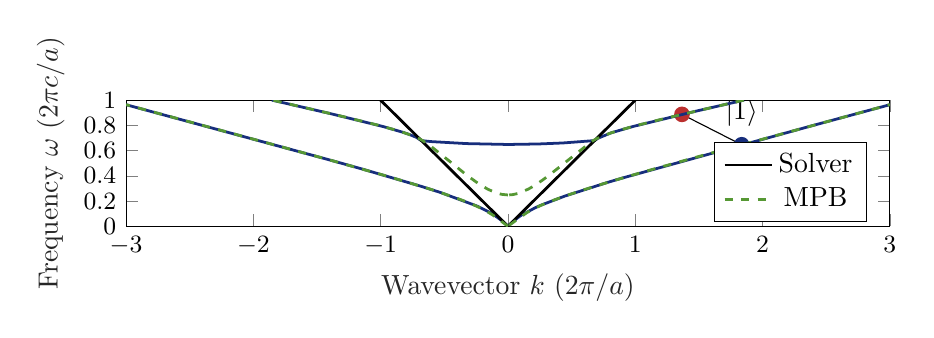
\begin{tikzpicture}

\begin{axis}[%
width=0.8\figW,
height=0.4\figH,
at={(0\figW,0\figH)},
scale only axis,
xmin=-3,
xmax=3,
xlabel style={font=\color{white!15!black}},
xlabel={Wavevector $k$ ($2 \pi /a$)},
ymin=0,
ymax=1,
ylabel style={font=\color{white!15!black}},
ylabel={Frequency $\omega$ ($2\pi c/a$)},
axis background/.style={fill=white},
legend pos=south east
]
%\draw[dashed] (-3,0.6468) -- (3,0.6468);
%\draw[dashed] (-3,0.8879) -- (3,0.8879);
%\node at (2.8,0.767) {$\Omega$};
%\draw[dashed] (1.836,0.6468) -- (1.836,0);
%\draw[dashed] (1.367,0.8879) -- (1.367,0);
\draw[->] (1.836,0.6468) -- (1.367,0.8879);
\node[label={90:{$\ket{1}$}},circle,fill=mode1,inner sep=2pt] at (1.836,0.6468) {};
\node[label={90:{$\ket{2}$}},circle,fill=mode2,inner sep=2pt] at (1.367,0.8879) {};
%\node[label={180:{}},circle,fill=mode3,inner sep=2pt] at (-2.305,0.8879) {};
\addplot [color=mode1, forget plot, line width=1.0pt]
table[row sep=crcr]{%
	-0	0\\
	-0.0425483776636622	0.04\\
	-0.112747396858924	0.0920000000000001\\
	-0.138703575229707	0.108\\
	-0.242619225661566	0.16\\
	-0.530251013303014	0.268\\
	-0.68277422737238	0.317\\
	-1.13395473723024	0.451\\
	-1.40367460079584	0.527\\
	-3.00095872332965	0.965\\
};
\addlegendentry{Solver};
\addplot [color=mode1, forget plot, line width=1.0pt]
table[row sep=crcr]{%
	-0	0.649\\
	-0.326077818628705	0.656\\
	-0.605487195406852	0.672\\
	-0.681620546537656	0.68\\
	-0.720361604419702	0.706\\
	-0.780889623877291	0.731\\
	-0.822707823290201	0.745\\
	-0.979328562522052	0.791\\
	-1.40286353275794	0.896\\
	-1.58333534884432	0.938\\
	-1.73350139501897	0.973\\
	-1.85486453299797	1.001\\
};
\addplot [color=mode1, forget plot, line width=1.0pt]
  table[row sep=crcr]{%
0.00856527091199988	0.0089999999999999\\
0.0355740339675572	0.0329999999999999\\
0.0773642883861596	0.0680000000000001\\
0.108965071776361	0.0899999999999999\\
0.216446056096282	0.148\\
0.266469085354788	0.17\\
0.44579687604775	0.239\\
0.779460193245421	0.347\\
0.90346776025157	0.384\\
2.38185947042077	0.796\\
3.00095872332965	0.965\\
};
\addplot [color=mode1, forget plot, line width=1.0pt]
  table[row sep=crcr]{%
0	0.649\\
0.241290268767007	0.653\\
0.432426865263543	0.661\\
0.681620546537656	0.68\\
0.70634705751922	0.698\\
0.812185645324833	0.742\\
0.983207321695099	0.792\\
1.48370503209761	0.915\\
1.85486453299797	1.001\\
};
\addplot [name path=A, color=black, line width=1.0pt]
  table[row sep=crcr]{%
0.00996678000000006	0.00996678000000006\\
1.00664	1.00664\\
};
\addplot [color=mode3, dashed, line width=1.0pt]
  table[row sep=crcr]{%
0.00996678000000006	0.00783098999999998\\
0.149502	0.108661\\
0.199336	0.137065\\
0.259136	0.166038\\
0.33887	0.199306\\
0.448505	0.239874\\
0.598007	0.290189\\
0.797342	0.352394\\
1.07641	0.434535\\
1.48505	0.549875\\
3	0.965172\\
};
\addlegendentry{MPB};
\addplot [color=mode3, dashed, line width=1.0pt, forget plot]
  table[row sep=crcr]{%
0.00996678000000006	0.248465\\
0.0398670999999999	0.251399\\
0.0797342000000001	0.260564\\
0.159468	0.294355\\
0.209302	0.32355\\
0.269103	0.364287\\
0.33887	0.417217\\
0.657807	0.673008\\
0.697674	0.695525\\
0.747508	0.71813\\
0.807309	0.740237\\
0.89701	0.768316\\
1.02658	0.803978\\
1.22591	0.85408\\
1.85382	1.00166\\
};
\addplot [name path=B, line width=1.0pt, color=black]
  table[row sep=crcr]{%
0	0\\
-1.00664	1.00664\\
};

\addplot [color=mode3, dashed, forget plot, line width=1.0pt]
  table[row sep=crcr]{%
-0	0\\
-0.119601	0.0893928000000002\\
-0.199336	0.137065\\
-0.289037	0.179054\\
-0.418605	0.229214\\
-0.61794	0.296612\\
-0.92691	0.391046\\
-1.42525	0.533211\\
-2.51163	0.831749\\
-3	0.965172\\
};
\addplot [color=mode3, dashed, forget plot, line width=1.0pt]
  table[row sep=crcr]{%
-0	0.248268\\
-0.0498339000000001	0.253143\\
-0.0996678	0.267229\\
-0.159468	0.294355\\
-0.229236	0.336534\\
-0.318937	0.401633\\
-0.458472	0.515573\\
-0.627907	0.653101\\
-0.687708	0.690319\\
-0.757475	0.722111\\
-0.857143	0.756346\\
-1.02658	0.803978\\
-1.33555	0.880479\\
-1.85382	1.00166\\
};
\end{axis}



\end{tikzpicture}%
	\caption[Dispersion for a waveguide of width $0.22  \mskip3mu \mu m$ and relative permittivity $12.25$.]{Dispersion relation for the waveguide of width $0.22  \mskip3mu \mu m$ and relative permittivity $\epsilon=12.25$, compared between the analytic solver and the open-source \textit{MPB}.}
	\label{fig:bandfinal}
\end{figure} 

Having extensively validated the implementation of the frequency domain method, non-reciprocal mode transition is now demonstrated for a spatio-temporal direct permittivity modulation. The simulation is chosen to be a thin slab dielectric waveguide of width $0.22  \mskip3mu \mu m$ and permittivity $\epsilon = 12.25$, corresponding to that of silicon. This particular waveguide is chosen as it possesses highly parallel bands in the dispersion relation (Fig \ref{fig:bandfinal}). Being parallel, there will almost always be a phase-matched pair of modes in the forward ($+k$) direction. So that for any even mode $\ket{1}$, a single modulation profile will ensure a transition to a corresponding odd mode $\ket{2}$ over a wide range of frequencies. This is ideal from an optical isolation point of view, which requires an ideally infinite frequency operation range. Likewise, in the backward propagating direction ($-k$), there is no single phase-matched pair of modes for a transition. Thus, a single modulation between the even and odd modes on this choice of waveguide provides highly \textit{broadband} optical isolation.

The simulation is run for an even and odd mode pair at frequencies $\omega_1 = 0.647 \mskip3mu  (2 \pi c/a)$ and $\omega_2 = 0.8879 \mskip3mu  (2\pi c/a)$ respectively, chosen from the calculated dispersion relation of Figure \ref{fig:bandfinal}. These modes have corresponding wavevectors $k_1 = 1.189 \mskip3mu  (2 \pi /a)$ and $k_2 = 0.912  \mskip3mu (2 \pi/a)$. A permittivity modulation of the form $\epsilon(x,t)' = \delta \cos (\Omega t + \Lambda x)$ is applied between $2.5  \mskip3mu \mu m$ and $7.5  \mskip3mu \mu m$ ($L_c = 5  \mskip3mu \mu m$) where $\Omega = \omega_2-\omega_1$ is the modulation frequency and $\Lambda = k_2 - k_1$. The upper and lower halves of the waveguide have a $\pi$ phase difference. The coherence length was determined by extending the modulation over a wider range and sampling the mode amplitudes as usual, with a strong modulation of $\delta = 1$. A modal source is excited at $1  \mskip3mu \mu m$, and frequencies are extracted at positions $D_1 = 1.5 \mskip3mu  \mu m$ and $D_2 = 9 \mskip3mu  \mu m$ over 5 sidebands at a spatial discretisation of $\Delta = 0.04  \mskip3mu \mu m$.

%% This file was created by matlab2tikz.
%
%The latest updates can be retrieved from
%  http://www.mathworks.com/matlabcentral/fileexchange/22022-matlab2tikz-matlab2tikz
%where you can also make suggestions and rate matlab2tikz.
%
\definecolor{mycolor1}{rgb}{0.00000,0.44700,0.74100}%
\definecolor{mycolor2}{rgb}{0.85000,0.32500,0.09800}%
\definecolor{mycolor3}{rgb}{0.92900,0.69400,0.12500}%
\definecolor{mycolor4}{rgb}{0.49400,0.18400,0.55600}%
%
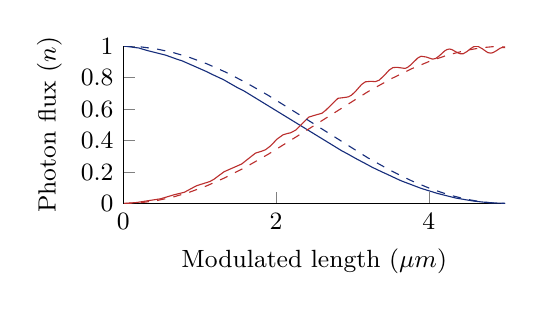
\begin{tikzpicture}

\begin{axis}[%
width=0.4\figW,
height=0.5\figH,
at={(0\figW,0\figH)},
scale only axis,
xmin=0,
xmax=5,
ymin=0,
ymax=1,
xlabel = {Modulated length ($\mu m$)},
ylabel = {Photon flux ($n$)},
axis background/.style={fill=white},
axis x line*=bottom,
axis y line*=left
]
\addplot [color=mode1]
  table[row sep=crcr]{%
0.00999999999999979	1\\
0.13	0.992\\
0.2	0.988\\
0.29	0.975\\
0.35	0.967\\
0.55	0.943\\
0.7	0.917\\
0.77	0.906\\
1.08	0.84\\
1.15	0.823\\
1.31	0.787\\
1.49	0.737\\
1.58	0.715\\
2.86	0.335\\
2.93	0.317\\
3.07	0.279\\
3.15	0.259\\
3.26	0.23\\
3.39	0.2\\
3.44	0.189\\
3.59	0.155\\
3.64	0.144\\
3.9	0.0961999999999996\\
4.11	0.0646000000000004\\
4.35	0.0351999999999997\\
4.59	0.0152999999999999\\
4.8	0.00460999999999956\\
5.01	0.00107000000000035\\
};
\addplot [color=mode2]
  table[row sep=crcr]{%
0.00999999999999979	0.00076699999999974\\
0.17	0.00628000000000029\\
0.49	0.0303000000000004\\
0.66	0.0549999999999997\\
0.8	0.0716000000000001\\
0.9	0.0978000000000003\\
0.96	0.113\\
1.05	0.127\\
1.13	0.139\\
1.19	0.155\\
1.25	0.177\\
1.32	0.202\\
1.55	0.251\\
1.73	0.32\\
1.81	0.332\\
1.86	0.341\\
1.92	0.363\\
1.96	0.382\\
2.01	0.408\\
2.09	0.436\\
2.15	0.445\\
2.19	0.449\\
2.26	0.467\\
2.31	0.491\\
2.43	0.549\\
2.51	0.561\\
2.6	0.573\\
2.65	0.592\\
2.81	0.668\\
2.92	0.675\\
2.95	0.678\\
2.99	0.689\\
3.04	0.712\\
3.12	0.756\\
3.17	0.773\\
3.24	0.776\\
3.3	0.774\\
3.35	0.783\\
3.42	0.815\\
3.48	0.847\\
3.53	0.863\\
3.58	0.865\\
3.69	0.858\\
3.72	0.864\\
3.76	0.879\\
3.86	0.926\\
3.9	0.935000000000001\\
3.96	0.931\\
4.05	0.917\\
4.09	0.921\\
4.14	0.939\\
4.21	0.97\\
4.24	0.978\\
4.27	0.981\\
4.3	0.978\\
4.36	0.962\\
4.41	0.951\\
4.45	0.951\\
4.5	0.965\\
4.54	0.981\\
4.59	0.997\\
4.64	0.999\\
4.7	0.983\\
4.77	0.959\\
4.81	0.955\\
4.84	0.958\\
4.88	0.969\\
4.93	0.985\\
4.96	0.991\\
4.99	0.991\\
5.01	0.988\\
};
\addplot [color=mode1, dashed]
  table[row sep=crcr]{%
0.00999999999999979	0.999990209\\
0.22	0.99526858\\
0.43	0.982005207\\
0.64	0.96042884\\
0.86	0.929316078\\
1.09	0.888113089\\
1.33	0.836575682\\
1.6	0.769602103\\
1.9	0.686271286\\
2.29	0.568622403\\
3.2	0.290741175\\
3.51	0.207120884\\
3.78	0.143143349\\
4.02	0.094757081\\
4.25	0.0569368749999999\\
4.47	0.0293268749999998\\
4.68	0.0112758949999998\\
4.89	0.00165378700000041\\
5.01	9.7910900000997e-06\\
};
\addplot [color=mode2, dashed]
  table[row sep=crcr]{%
0.00999999999999979	9.7910900000997e-06\\
0.22	0.00473141999999971\\
0.43	0.0179947929999997\\
0.64	0.0395711600000004\\
0.86	0.0706839219999997\\
1.09	0.111886911\\
1.33	0.163424318\\
1.6	0.230397897\\
1.9	0.313728714\\
2.29	0.431377597\\
3.2	0.709258825\\
3.51	0.792879116\\
3.78	0.856856651\\
4.02	0.905242919\\
4.25	0.943063125\\
4.47	0.970673125\\
4.68	0.988724105\\
4.89	0.998346213\\
5.01	0.999990209\\
};
\end{axis}
\end{tikzpicture}%
Figure \ref{fig:bandyu} shows the results of the simulation for the forward, backward, and time-reversed simulations. Only the total combined field of all sidebands is shown ($\sum E_z(\omega_n)$), as opposed to each individual sideband. The system exhibits a strongly non-reciprocal response - on the left to right path, the mode completely converts from $\ket{1}$ to $\ket{2}$. However, on the right to left direction the modulation does not cause a transition since there is no corresponding point on the dispersion relation for the mode to `jump'. Similarly, on the time-reversed path the modulation does not transition the odd mode to the second even mode (the third band on the dispersion relation). These non-reciprocal mode conversions can be removed using standard modal filters, allowing for complete isolation \cite{Lee2003,Jiao2005}.

\begin{figure}[t]
	\centering
	\setlength{\figH}{0.4\textwidth}
	\setlength{\figW}{\textwidth}
	\begin{subfigure}[t]{0.5\textwidth}
		% This file was created by matlab2tikz.
%
%The latest updates can be retrieved from
%  http://www.mathworks.com/matlabcentral/fileexchange/22022-matlab2tikz-matlab2tikz
%where you can also make suggestions and rate matlab2tikz.
%
\begin{tikzpicture}

\begin{axis}[%
width=0.35\figW,
height=0.2\figH,
at={(0\figW,0.75\figW)},
scale only axis,
point meta min=-1,
point meta max=1,
axis on top,
clip=false,
xmin=0,
xmax=10,
ymin=0,
ymax=1,
xlabel = {x ($\mu m$)},
ytick={0,0.5,1},
yticklabels={$0$,$0.5$, $1$},
ylabel={$\text{y (}\mu\text{m)}$},
axis background/.style={fill=white},
colormap={mymap}{[1pt] rgb(0pt)=(0,0,1); rgb(31pt)=(1,1,1); rgb(32pt)=(1,1,1); rgb(63pt)=(1,0,0)},
colorbar,
colorbar style={width=.02\linewidth, at={(1.05,0.1\figH)}, anchor=east,ytick={-1,1}},
colorbar style={title={$V / \mu m$}}
]
\addplot graphics [xmin=0, xmax=10, ymin=0, ymax=1] {graphs/fdtd/phasematch/LR/field-1.png};
\node at (-1,2) {\textbf{(a)}};
\node at (2,1.2) {$\ket{1} \rightarrow$};
\node at (8,1.2) {$\rightarrow \ket{2}$};
\end{axis}

\begin{axis}[%
width=0.35\figW,
height=0.2\figH,
at={(0\figW,0.5\figW)},
scale only axis,
point meta min=-1,
point meta max=1,
axis on top,
xmin=0,
clip=false,
xmax=10,
ymin=0,
ymax=1,
xlabel = {x ($\mu m$)},
ytick={0,0.5,1},
yticklabels={$0$,$0.5$, $1$},
ylabel={$\text{y (}\mu\text{m)}$},
axis background/.style={fill=white},
colormap={mymap}{[1pt] rgb(0pt)=(0,0,1); rgb(31pt)=(1,1,1); rgb(32pt)=(1,1,1); rgb(63pt)=(1,0,0)},
colorbar,
colorbar style={width=.02\linewidth, at={(1.05,0.1\figH)}, anchor=east,ytick={-1,1}}
]
\addplot [forget plot] graphics [xmin=0, xmax=10, ymin=0, ymax=1] {graphs/fdtd/phasematch/RL/fieldRL-1.png};
\node at (-1,2) {\textbf{(b)}};
\node at (2,1.2) {$\bra{1} \leftarrow$};
\node at (8,1.2) {$\leftarrow \bra{1}$};
\end{axis}

\begin{axis}[%
width=0.35\figW,
height=0.2\figH,
at={(0\figW,0.25\figW)},
scale only axis,
point meta min=-1,
point meta max=1,
axis on top,
xmin=0,
xmax=10,
ymin=0,
ymax=1,
ytick={0,0.5,1},
clip=false,
xlabel = {x ($\mu m$)},
yticklabels={$0$,$0.5$, $1$},
ylabel={$\text{y (}\mu\text{m)}$},
axis background/.style={fill=white},
colormap={mymap}{[1pt] rgb(0pt)=(0,0,1); rgb(31pt)=(1,1,1); rgb(32pt)=(1,1,1); rgb(63pt)=(1,0,0)},
colorbar,
colorbar style={width=.02\linewidth, at={(1.05,0.1\figH)}, anchor=east,ytick={-1,1}}
]
\addplot [forget plot] graphics [xmin=0, xmax=10, ymin=0, ymax=1] {graphs/fdtd/phasematch/TR/fieldTR-1.png};
\node at (-1,2) {\textbf{(c)}};
\node at (2,1.2) {$\bra{2} \leftarrow$};
\node at (8,1.2) {$\leftarrow \bra{2}$};
\end{axis}
\end{tikzpicture}%
	\end{subfigure}%
	\begin{subfigure}[t]{0.5\textwidth}
		% This file was created by matlab2tikz.
%
%The latest updates can be retrieved from
%  http://www.mathworks.com/matlabcentral/fileexchange/22022-matlab2tikz-matlab2tikz
%where you can also make suggestions and rate matlab2tikz.
%
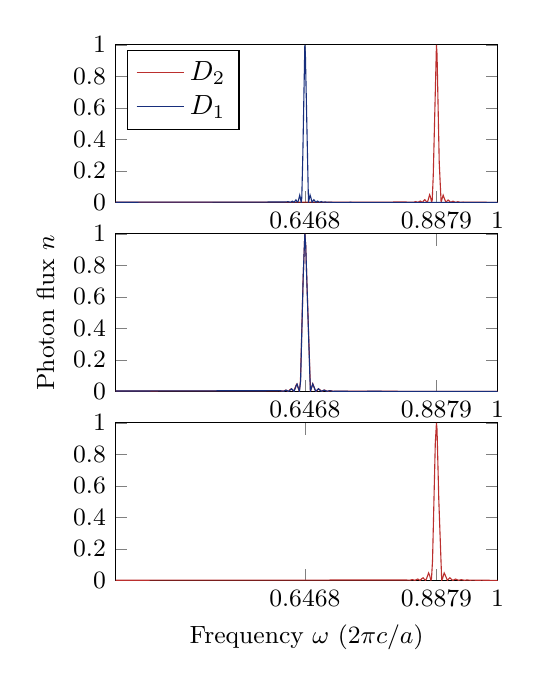
\begin{tikzpicture}

\begin{axis}[%
width=0.4\figW,
height=0.5\figH,
at={(0\figW,1.2\figH)},
scale only axis,
xmin=0.3,
xmax=1,
xtick={0,0.6468,0.8879,1},
xticklabels={$0$,$0.6468$, $0.8879$,$1$},
ymin=0,
ymax=1,
axis background/.style={fill=white},
legend pos = north west
]
\addplot [color=mode2]
  table[row sep=crcr]{%
0	1.13081867070264e-06\\
0.831674911128847	0.00228169467746064\\
0.838881336867126	0.00202377499498518\\
0.842618002064753	0.0021823789198463\\
0.845820857948432	0.000498850577067556\\
0.849824427803032	0.00520157028131374\\
0.853827997657632	0.000158448678008183\\
0.858365376826178	0.00870591815290878\\
0.862102042023805	5.71739905264046e-05\\
0.865304897907484	0.0133645158166602\\
0.866639421192351	0.0173069295692947\\
0.869041563105111	0.00685264541172503\\
0.870642991046951	5.45500426432088e-05\\
0.872244418988791	0.00968327963340587\\
0.87544727487247	0.048612317596354\\
0.87704870281431	0.0344557748770749\\
0.879183940070097	0.000143863495585039\\
0.88025155869799	0.0162957894625595\\
0.882119891296803	0.170638303761119\\
0.887991793750216	1\\
0.889059412378109	0.94000608315541\\
0.893062982232709	0.255338855812756\\
0.896532742773362	4.8698814648418e-05\\
0.898134170715202	0.0209729769593403\\
0.900269407970989	0.0458723635961076\\
0.902404645226775	0.0252393913145816\\
0.905340596453482	9.65076844801072e-05\\
0.909344166308081	0.0156763040359307\\
0.914148450133601	0.000139489728146369\\
0.918152019988201	0.00780486864007757\\
0.92295630381372	0.000160502704093402\\
0.927226778325293	0.00448871207940704\\
0.932031062150813	0.00033301513591999\\
0.936835345976332	0.00232446948495424\\
0.941639629801852	0.000858887074389303\\
0.946177008970398	0.00117400414562741\\
0.950981292795918	0.00101797533071468\\
0.962458193045771	0.00106641777035499\\
0.969397714127077	0.000883365111032708\\
1.00196008227782	0.000118551983291804\\
1.02357935949266	0.000217825320773857\\
1.05854386955616	0.000104712082806824\\
1.15596406935142	4.98964502413379e-05\\
1.3342563802096	7.9476366254827e-06\\
};
\addlegendentry{$D_2$};
\addplot [color=mode1]
  table[row sep=crcr]{%
0	1.39644351637713e-08\\
0.609076427213103	0.00233545672979218\\
0.616282852951382	0.00430043014561177\\
0.620553327462955	0.000248637961077769\\
0.623756183346635	0.00794154826945515\\
0.626959039230315	7.47971153032267e-05\\
0.630428799770968	0.0162317707623461\\
0.632830941683728	0.00204526366888014\\
0.634699274282541	0.00886138610265252\\
0.637368320852274	0.0457755204955326\\
0.638969748794114	0.0193771513115848\\
0.640037367422007	0.000188198916072357\\
0.641104986049901	0.0271105460388243\\
0.642973318648714	0.289533327408285\\
0.64670998384634	1\\
0.647777602474233	0.934370010222459\\
0.653382600270673	0.00025932622168523\\
0.654717123555539	0.0216863788474451\\
0.656318551497379	0.0470796939868294\\
0.657653074782246	0.0325194712216197\\
0.660055216695006	3.53592225057486e-05\\
0.663258072578686	0.0169734429174946\\
0.666994737776312	8.14290493287295e-05\\
0.669930689003018	0.00862561475450141\\
0.673667354200645	4.6983461483352e-05\\
0.676870210084324	0.00514223972653949\\
0.680606875281951	0.000200359717916987\\
0.683809731165631	0.00342867981165518\\
0.687546396363257	0.000316680510486389\\
0.69101615690391	0.00206216482641941\\
0.69501972675851	0.000905361107496283\\
0.699557105927056	0.000132641242323706\\
0.706496627008362	3.5452938580427e-05\\
0.713436148089669	9.90346817442145e-07\\
0.720642573827948	4.63588478374355e-05\\
0.730251141478987	0.000719353650030063\\
0.741461137071867	0.000186432024472216\\
0.758276130461185	0.000260226636216387\\
0.782297549588784	0.00020597772171671\\
1.3342563802096	1.2617425668715e-06\\
};
\addlegendentry{$D_1$};
\end{axis}

\begin{axis}[%
width=0.4\figW,
height=0.5\figH,
at={(0\figW,0.6\figH)},
scale only axis,
xmin=0.3,
xmax=1,
xtick={0,0.6468,0.8879,1},
xticklabels={$0$,$0.6468$, $0.8879$,$1$},
ymin=0,
ymax=1,
axis background/.style={fill=white},
ylabel={Photon flux $n$}
]
\addplot [color=mode2]
table[row sep=crcr]{%
	0	2.23814667652533e-05\\
	0.599467859562064	0.00433628591280777\\
	0.607208094614289	0.00142683721257098\\
	0.611478569125863	0.00804573548853171\\
	0.616015948294409	2.38495126281268e-05\\
	0.621620946090848	0.0165221829549806\\
	0.626425229916368	0.000103599094986251\\
	0.630695704427941	0.0391146642895677\\
	0.632030227712808	0.0463381738836528\\
	0.634966178939514	0.0150116981517305\\
	0.636567606881354	0.000103582077880748\\
	0.638702844137141	0.0650888340040292\\
	0.64350712796266	0.709716332149051\\
	0.64670998384634	1\\
	0.64831141178818	0.928598166077518\\
	0.657119265468299	5.24822337082398e-05\\
	0.661389739979872	0.0480230679381304\\
	0.665660214491445	0.00758763999999168\\
	0.667528547090259	6.15704802147121e-05\\
	0.672065926258805	0.0163909949062666\\
	0.677937828712218	0.000108656655533057\\
	0.682742112537738	0.00847027912289966\\
	0.688347110334177	9.69307907228156e-05\\
	0.693685203473643	0.00469925536614135\\
	0.699290201270083	0.000427018840210458\\
	0.706763531665336	0.000799353937359193\\
	0.73692375790332	0.000616286557307388\\
	1.04172887616684	6.40938787921375e-05\\
	1.3342563802096	8.46451827918315e-06\\
};
\addplot [color=mode1]
table[row sep=crcr]{%
	0	1.56938971469511e-05\\
	0.601069287503903	0.00451669176492464\\
	0.60800880858521	0.000851375047454139\\
	0.612279283096783	0.00805966375870093\\
	0.617083566922302	9.43746109351995e-05\\
	0.622421660061768	0.0163816251332891\\
	0.626959039230315	4.73278638151164e-05\\
	0.630962609084915	0.0368452763636986\\
	0.632564037026754	0.0462407726858916\\
	0.636834511538327	2.87090439536897e-05\\
	0.638969748794114	0.0661715327694608\\
	0.643774032619634	0.733609777486815\\
	0.64670998384634	1\\
	0.64831141178818	0.926810610112689\\
	0.656852360811326	8.02636681402902e-05\\
	0.661122835322899	0.0475272659011989\\
	0.666727833119339	8.47098536960189e-06\\
	0.671532116944858	0.0167160835620319\\
	0.676870210084324	1.7232287029989e-05\\
	0.681674493909844	0.008387982526882\\
	0.687279491706284	0.000175526652539837\\
	0.692350680188777	0.0048707240118413\\
	0.697688773328243	0.000322623719081649\\
	0.704895199066522	0.000921248344013526\\
	0.73532232996148	0.000254606514388689\\
	0.772955886594717	0.000574892630722301\\
	0.819664201565048	0.000238753269072856\\
	1.06735172323628	5.2218821191552e-06\\
	1.3342563802096	1.2676653494248e-05\\
};
\end{axis}


\begin{axis}[%
width=0.4\figW,
height=0.5\figH,
at={(0\figW,0\figH)},
scale only axis,
xlabel = {Frequency $\omega$ ($2 \pi c/a$)},
xmin=0.3,
xmax=1,
xtick={0,0.6468,0.8879,1},
xticklabels={$0$,$0.6468$, $0.8879$,$1$},
ymin=0,
ymax=1,
axis background/.style={fill=white}
]
\addplot [color=mode2]
table[row sep=crcr]{%
	0	1.22034047884689e-05\\
	0.8311411018149	0.0023013266385894\\
	0.835411576326473	0.00175360932962421\\
	0.839415146181073	0.000965341281125021\\
	0.843685620692646	0.00486553930555145\\
	0.848489904518166	0.000250045011197297\\
	0.853561093000659	0.00825574609007673\\
	0.858098472169205	4.97169960933519e-05\\
	0.861301328052885	0.0109829985996603\\
	0.863436565308671	0.0163494616861442\\
	0.866372516535378	0.00457764465273192\\
	0.867973944477217	1.94703586926526e-05\\
	0.870109181733004	0.013154486929305\\
	0.873578942273657	0.0470453003425026\\
	0.87544727487247	0.0315310399247428\\
	0.87784941678523	2.28975304077395e-05\\
	0.878917035413123	0.0124357545233098\\
	0.880785368011937	0.12400183153239\\
	0.885856556494429	0.869270322219562\\
	0.887991793750216	1\\
	0.889059412378109	0.957556042194106\\
	0.892262268261789	0.513878092808121\\
	0.897600361401255	0.00108842262365672\\
	0.899201789343095	0.0122024441442494\\
	0.902137740569802	0.047153720606177\\
	0.904272977825588	0.0315377211631087\\
	0.908009643023215	1.99441444377335e-05\\
	0.912547022191761	0.0164419581043247\\
	0.916016782732414	0.0041292680012357\\
	0.918152019988201	5.37346492168744e-05\\
	0.92295630381372	0.00824687137239732\\
	0.92856130161016	0.000227034194552944\\
	0.933632490092653	0.00460027207861069\\
	0.938970583232119	0.000392405550539987\\
	0.944308676371585	0.00264766067464928\\
	0.949646769511052	0.000683950981152037\\
	0.954717957993545	0.00165690344143354\\
	0.960056051133011	0.000724562177670807\\
	0.965394144272477	0.000892302126201283\\
	0.97126604672589	0.0010733450416256\\
	0.986212707516396	0.000294720956906636\\
	1.00943341267307	0.000131287278812842\\
	1.02411316880661	0.00048471950436868\\
	1.04066125753895	0.000233818595714919\\
	1.06841934186418	6.61720048844572e-06\\
	1.10391766124163	0.000200101820605481\\
	1.14662240635736	3.20710461947371e-05\\
	1.3342563802096	4.61615482860722e-05\\
};
\end{axis}
\end{tikzpicture}%
	\end{subfigure}
	\caption[Non-reciprocal frequency conversion in a strongly modulated waveguide]{Phase matched non-reciprocal mode conversion in a modulated structure for \textbf{a)} LR, \textbf{b)} LR, and \textbf{c)} TR directions. On the left are the $E_z$ fields, and on the right are the corresponding frequencies for detectors $D_1$ and $D_2$. Note that in all the Fourier graphs, results are shown for both detectors. However, in the case of the $RL$ and $TR$ directions, the input and output are identical.}
	\label{fig:bandyu}
\end{figure} 


\section{Optical isolation through a photonic AB effect}
\label{sec:opticAB}

\begin{figure}[t!]
	\centering
	\setlength{\figH}{1\textwidth}
	\setlength{\figW}{1\textwidth}
	
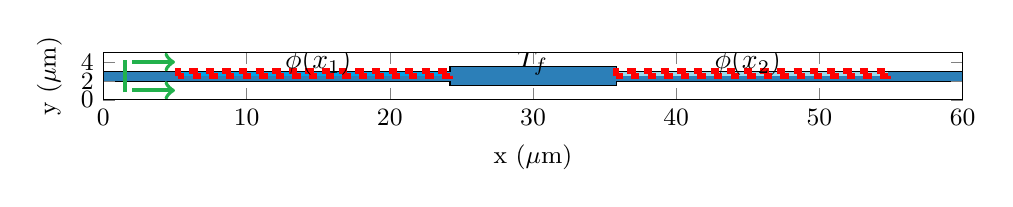
\begin{tikzpicture}
    \begin{axis}[%
width=0.9\figW,
height=0.15\figH,
at={(0\figW,0\figH)},
scale only axis,
axis on top,
xmin=0,
xmax=60,
xlabel={$\text{x (}\mu\text{m)}$},
ymin=0,
ymax=5,
ylabel={$\text{y (}\mu\text{m)}$},
axis background/.style={fill=white},
]
\fill[fill=eps] (0,1.95) rectangle (60,3.05);
\fill[fill=eps] (24.2,1.5) rectangle (35.8,3.5);
\fill[fill=modup] (5.2,2.5) rectangle (24.2,3.05);
\fill[fill=moddown] (35.8,2.5) rectangle (54.8,3.05);
\draw (0,1.95) -- (24.2,1.95) -- (24.2,1.5) -- (35.8,1.5) -- (35.8,1.95) -- (60,1.95);
\draw (0,3.05) -- (24.2,3.05) -- (24.2,3.5) -- (35.8,3.5) -- (35.8,3.05) -- (60,3.05);
\draw[draw=src, line width=0.5mm] (1.5,0.8) -- (1.5,4.2);
\draw[line width=0.5mm, draw=src, ->] (2,4) -- (5,4);
\draw[line width=0.5mm, draw=src, ->] (2,1) -- (5,1);
\draw[dashed, draw=red, line width=0.7mm] (5.2,2.5) -- (5.2,3.05) -- (24.2,3.05) -- (24.2,2.5) -- (5.2,2.5);
\draw[dashed, draw=red, line width=0.7mm] (35.8,2.5) -- (35.8,3.05) -- (54.8,3.05) -- (54.8,2.5) -- (35.8,2.5);
\node at (15,4) {$\phi(x_1)$};
\node at (45,4) {$\phi(x_2)$};
\node at (30,4) {$T_f$};
\end{axis}
\end{tikzpicture}%
	\caption[Waveguide for demonstrating a photonic AB effect]{The modulated waveguide structure for demonstrating a photonic Aharonov-Bohm effect. The dark blue region is a material of unity permeability and relative permittivity $\epsilon = 12.25$. The light blue sections enclosed in dashed red lines are regions where the permittivity is modulated by an amount $0.1 \epsilon \cos(\omega t + \phi)$, with $\phi(x_1)$ on the left and $\phi(x_2)$ on the right. The green line indicates the region over which the modal source is injected, in this case, from left to right (LR). The central waveguide imparts a mode-dependent phase on light passing through it, described by the transfer matrix $T_f$.}%
	\label{fig:abcavity}
\end{figure}

The difficulty in applying spatio-temporal modulations for the purpose of optical isolation is that the spatial dependence of the modulation is highly difficult to engineer. Currently, such modulations are created by simultaneously controlling the permittivity of hundreds of discrete points in a waveguide at different phases. However, without the wavevector shift the mode transition is purely reciprocal, as modes propagating in the reverse direction are still phase-matched (the transition on the dispersion relation is completely vertical, and so the modulation does not discriminate between left and right propagating modes). Here, based on the work of Fang et al. \cite{Fang2012}, a broadband tunable optical isolator is constructed and simulated in the frequency domain using only the gauge potential that emerges from the phase of \textit{temporal} dynamic modulations, as discussed in Section \ref{sec:gauge}. The choice of a direct transition marks the ideal configuration for a modulation, as only two separate regions need to be modulated with no spatial dependence.

Consider first the structure of Figure \ref{fig:abcavity}, which consists of a single narrow waveguide connected to a central waveguide region. The narrow waveguide supports an even and odd mode $\ket{1}$ and $\ket{2}$ respectively. A modulation of the form
\begin{equation}
\epsilon(t)' = \delta \cos (\Omega t + \phi(x_1))
\end{equation}
is applied on the left side of the waveguide, and another modulation 
\begin{equation}
\epsilon(t)' = \delta \cos (\Omega t + \phi(x_2))
\end{equation}
on the right side to induce reciprocal transitions between the modes. The central waveguide region can be chosen to impart a mode-dependent phase on light passing through it, so there are effectively two pathways through which light can propagate. The transfer matrix for modes passing through the central waveguide is then 

\begin{equation}
T_f =
\begin{bmatrix}
e^{i \phi(P_1)} & 0 \\
0 & e^{i \phi(P_2)} 
\end{bmatrix}.
\end{equation}

In the second path ($P_2$), a photon of mode $\ket{1}$ is injected from the left and undergoes a transition to state $\ket{2}$, gaining an additional $\phi(x_1)$ phase. Upon passing through the central region, the photon acquires an additional phase $\phi(P_2)$, and undergoes a transition back to $\ket{1}$ in the second modulated region, gaining a final $-\phi(x_2)$ phase. In the first path ($P_1$), the initial mode is no longer converted and only acquires a $\phi(P_1)$ phase from the central waveguide region.

Thus, the total phase difference between the two pathways is then 

\begin{equation}
\Delta \phi_{LR} = \phi(P_2) - \phi(P_1) + \phi(x_1) - \phi(x_2).
\end{equation}
Likewise, in the right to left direction the total phase difference is instead
\begin{equation}
\Delta \phi_{RL} =  \phi(P_2) - \phi(P_1) + \phi(x_2) - \phi(x_1),
\end{equation}
which is identical to the discussion of the photonic Aharonov-Bohm effect of Section \ref{sec:opticAB}. In this case, the two modulated regions play the role of the separate interferometer arms, with the path-dependent phase of the central waveguide being equivalent to the phase acquired by an electron passing through a magnetic vector potential $\bm{A}$. 

Because of this, despite the nature of the direct modulation itself being reciprocal, the gauge potential can be designed to generate non-reciprocal phases. In particular, non-reciprocal frequency conversion can be demonstrated without requiring a spatial modulation profile by choosing the phases so that $\phi(x_2)-\phi(x_1) = \pi/2$, and $\phi(P_2) - \phi(P_1) = \pi/2$. To allow for interference between modes, the modulated length is chosen as $L = 0.5 L_c$, so that only half of the mode will transition (50\% of the modal power will transition to the other mode). From these choices, the transfer matrix for modes propagating right to left is then

\begin{equation}
T_{LR} = T(\phi_2) T_f T(\phi_1) = e^{-i(2kL - \phi(P_1))} 
\begin{bmatrix}
0 & i \\
-1 & 0
\end{bmatrix},
\end{equation}

On the other hand, in the right to left direction the transfer matrix is instead given by

\begin{equation}
T_{RL} = T(\phi_1)T_f T(\phi_2) =  e^{-i(2kL - \phi(P_1))}
\begin{bmatrix}
1 & 0 \\
0 & i
\end{bmatrix}.
\end{equation}

From this, an even mode of state $\ket{1}$ injected from the left of the waveguide will completely convert to an odd mode $\ket{2}$, whereas the same even mode injected from the right will remain an even mode.

\begin{figure}[t]
	\centering
	\setlength{\figH}{\textwidth}
	\setlength{\figW}{\textwidth}
	% This file was created by matlab2tikz.
%
%The latest updates can be retrieved from
%  http://www.mathworks.com/matlabcentral/fileexchange/22022-matlab2tikz-matlab2tikz
%where you can also make suggestions and rate matlab2tikz.
%
\definecolor{mycolor1}{rgb}{0.00000,0.44700,0.74100}%
\definecolor{mycolor2}{rgb}{0.00000,0.44706,0.74118}%
\definecolor{mycolor3}{rgb}{0.46600,0.67400,0.18800}%
\definecolor{mycolor4}{rgb}{0.00000,0.49804,0.00000}%
%
\begin{tikzpicture}

\begin{axis}[%
width=0.8\figW,
height=0.4\figH,
at={(0\figW,0\figH)},
scale only axis,
xmin=0.001,
yticklabel style={/pgf/number format/fixed},
xticklabel style={/pgf/number format/fixed},
xmax=0.5,
xlabel={Wavevector $\text{k (2}\pi\text{/a)}$},
ymin=0,
ymax=0.25,
ylabel={Frequency $\omega\text{ (2}\pi\text{c/a)}$},
axis background/.style={fill=white},
legend pos=south east
]
\addplot [color=mycolor1, line width=1.0pt]
  table[row sep=crcr]{%
0.00106370944159151	0.001\\
0.0173164838778657	0.015\\
0.0339791004711106	0.025\\
0.0485238451323132	0.032\\
0.0840513505460331	0.046\\
0.161161500553998	0.0710000000000001\\
0.322500034364579	0.117\\
0.501279538435555	0.166\\
};
\addlegendentry{Solver};
\addplot [color=mycolor2, line width=1.0pt, forget plot]
  table[row sep=crcr]{%
0	0.129\\
0.060088932026341	0.131\\
0.129014261816538	0.135\\
0.137389857852266	0.137\\
0.140026562489592	0.139\\
0.158721291577674	0.147\\
0.187634882659275	0.156\\
0.230105681117631	0.167\\
0.292652360394282	0.182\\
0.374312220807439	0.201\\
0.503433266613461	0.231\\
};
\addplot [color=mycolor3, dashed, line width=1.0pt]
  table[row sep=crcr]{%
0	0\\
0.0348259	0.0222165\\
0.0557214	0.0333214000000001\\
0.0800995	0.0439132\\
0.111443	0.0552305\\
0.163682	0.071727\\
0.254229	0.0979683\\
0.431841	0.147035\\
0.501493	0.166061\\
};
\addplot [color=mycolor4, dashed, line width=1.0pt]
  table[row sep=crcr]{%
0	0.093062\\
0.0139303	0.0938928\\
0.0313433	0.0971598\\
0.0487562	0.102545\\
0.0731343	0.11255\\
0.132338	0.138462\\
0.160199	0.14803\\
0.198507	0.158972\\
0.264677	0.17542\\
0.445771	0.217557\\
0.501493	0.230556\\
};
\addlegendentry{MPB};
\addplot [color=black, line width=1.0pt]
  table[row sep=crcr]{%
0	0\\
0.250746	0.250746\\
};

\node[label={180:{$\ket{1}$}},circle,fill=mode1,inner sep=2pt] at (0.366,0.129) {};
\node[label={180:{$\ket{2}$}},circle,fill=mode2,inner sep=2pt] at (0.366,0.199) {};
\draw[line width=0.2mm, draw=black, ->] (0.366,0.135) -- (0.366,0.193);
\node[label={180:{$\Omega$}}] at (0.366,0.164) {};
\end{axis}
\end{tikzpicture}%
	\caption[Dispersion relation of a waveguide of width $1.1 \mu m$ and relative permittivity $12.25$.]{Dispersion relation of a waveguide with width $1.1 \mu m$ and relative permittivity $12.25$. Green dashes indicate dispersions obtained through \textit{MPB}, whereas blue lines indicate those calculated analytically using the purpose-written solver. The red line is the direct transition between modes $\ket{1}$ and $\ket{2}$. Since the modulation has no spatial dependence, the modulation does not discriminate between forward and backward propagating modes.}
	\label{fig:banddiagram}
\end{figure}


This is implemented in the frequency domain simulation by choosing the narrow waveguide to be of width $1.1  \mskip3mu \mu m$ extending from $0$ to $60 \mskip3mu  \mu m$, and the central waveguide region to be $2.2  \mskip3mu \mu m$ wide and $11.6 \mskip3mu  \mu m$ long, with relative permittivity $\epsilon = 12.25$. For the narrow waveguide, this choice corresponds to the dispersion relation of Figure \ref{fig:banddiagram}. The direct transition is induced between an even mode $\ket{1}$ chosen at $\omega_1 = 0.129 \mskip3mu (2 \pi c/a)$ and odd mode $\ket{2}$ at $\omega_2 = 0.199  \mskip3mu (2 \pi c/a)$, which share the same wavevector $k_{1,2} = 0.380 \mskip3mu  (2 \pi / a)$. To satisfy the modulation condition for the above transfer matrix, the waveguide is modulated on the left and right by $0.1 \epsilon \cos (\Omega t + \phi)$, with the phase of modulation set at $0$ and $\pi/2$ respectively ($\phi(x_2) - \phi(x_1) = \pi/2$). The choice of width for the central waveguide ($2 \mskip3mu \mu m$) ensures that even and odd modes acquire a $\pi/2$ phase difference upon passing through ($\phi(P_2) - \phi(P_1) = \pi/2$). The length of the modulated regions is half the coherence length ($19  \mskip3mu  \mu m$), so that a mode injected from the left will undergo a 50\% transition to the second mode, and vice versa. To test the non-reciprocal conversion, a modal source is excited at $1  \mskip3mu \mu m$ for the left to right direction, and $59 \mskip3mu  \mu m$ for the right to left and time-reversed directions. The simulation is performed over 3 sidebands at a spatial discretisation of $\Delta = 0.04 \mskip3mu  \mu m$, however only the first set of sidebands are shown.

\begin{figure}[t!]
	\centering
	\setlength{\figH}{1\textwidth}
	\setlength{\figW}{1\textwidth}
	% This file was created by matlab2tikz.
%
%The latest updates can be retrieved from
%  http://www.mathworks.com/matlabcentral/fileexchange/22022-matlab2tikz-matlab2tikz
%where you can also make suggestions and rate matlab2tikz.
%
\pgfplotsset{fangFields/.style={
	width=0.8\figW,
height=0.08\figH,
	scale only axis,
	axis on top,
	title style = {at={(0.4\figH,0.06\figH)}},
	xmin=0,
	xmax=60,
	ymin=0,
	clip=false,
	ymax=5,
	axis background/.style={fill=white},
	colormap={mymap}{[1pt] rgb(0pt)=(0,0,1); rgb(31pt)=(1,1,1); rgb(32pt)=(1,1,1); rgb(63pt)=(1,0,0)},
	colorbar,
	colorbar style={width=.01\linewidth, at={(1.02,0.04\figH)}, anchor=east}	
	}
}

\begin{tikzpicture}
\begin{axis}[%
fangFields,
at={(0\figW,0.95\figH)},
title = {Total field},
point meta min=-23,
point meta max=23,
xticklabels={,,},
colorbar style={title={$V / \mu m$}, width=.01\linewidth, at={(1.02,0.04\figH)}, anchor=east},
ylabel={$\text{y (}\mu\text{m)}$}
]
\addplot [forget plot] graphics [xmin=0, xmax=60, ymin=0, ymax=5] {graphs/fangcavity/LR/totalfield.png};
\draw (0,1.95) -- (24.2,1.95) -- (24.2,1.5) -- (35.8,1.5) -- (35.8,1.95) -- (60,1.95);
\draw (0,3.05) -- (24.2,3.05) -- (24.2,3.5) -- (35.8,3.5) -- (35.8,3.05) -- (60,3.05);
\node at (55,6) {$\longrightarrow \ket{2}$};
\node at (5,6) {$\ket{1} \longrightarrow$};
\node at (-2,7) {\textbf{(a)}};
\end{axis}

\begin{axis}[%
fangFields,
at={(0\figW,0.8\figH)},
title = {$\omega_1 - \Omega$},
point meta min=-0.11845616858408,
point meta max=0.11845616858408,
xticklabels={,,},
ylabel={$\text{y (}\mu\text{m)}$}
]
\addplot [forget plot] graphics [xmin=0, xmax=60, ymin=0, ymax=5] {graphs/fangcavity/LR/nameoffile2-1.png};
\draw (0,1.95) -- (24.2,1.95) -- (24.2,1.5) -- (35.8,1.5) -- (35.8,1.95) -- (60,1.95);
\draw (0,3.05) -- (24.2,3.05) -- (24.2,3.5) -- (35.8,3.5) -- (35.8,3.05) -- (60,3.05);
\end{axis}

\begin{axis}[%
fangFields,
at={(0\figW,0.65\figH)},
title = {$\omega_1$},
point meta min=-6.64719566790506,
point meta max=6.64719566790506,
xticklabels={,,},
ylabel={$\text{y (}\mu\text{m)}$}
]
\addplot [forget plot] graphics [xmin=0, xmax=60, ymin=0, ymax=5] {graphs/fangcavity/LR/nameoffile2-2.png};
\draw (0,1.95) -- (24.2,1.95) -- (24.2,1.5) -- (35.8,1.5) -- (35.8,1.95) -- (60,1.95);
\draw (0,3.05) -- (24.2,3.05) -- (24.2,3.5) -- (35.8,3.5) -- (35.8,3.05) -- (60,3.05);
\end{axis}

\begin{axis}[%
fangFields,
at={(0\figW,0.5\figH)},
title = {$\omega_1 + \Omega$},
point meta min=-10.2001641787316,
point meta max=10.2001641787316,
xlabel={$\text{x (}\mu\text{m)}$},
ylabel={$\text{y (}\mu\text{m)}$}
]
\addplot [forget plot] graphics [xmin=0, xmax=60, ymin=0, ymax=5] {graphs/fangcavity/LR/nameoffile2-3.png};
\draw (0,1.95) -- (24.2,1.95) -- (24.2,1.5) -- (35.8,1.5) -- (35.8,1.95) -- (60,1.95);
\draw (0,3.05) -- (24.2,3.05) -- (24.2,3.5) -- (35.8,3.5) -- (35.8,3.05) -- (60,3.05);
\node at (-2,-3) {\textbf{(b)}};
\end{axis}

% This file was created by matlab2tikz.
%
%The latest updates can be retrieved from
%  http://www.mathworks.com/matlabcentral/fileexchange/22022-matlab2tikz-matlab2tikz
%where you can also make suggestions and rate matlab2tikz.
%
%\definecolor{mycolor1}{rgb}{0.00000,0.44700,0.74100}%
%\definecolor{mycolor2}{rgb}{0.85000,0.32500,0.09800}%
%\definecolor{mycolor3}{rgb}{0.92900,0.69400,0.12500}%
%
\definecolor{mycolor1}{RGB}{0,128,0}%
\definecolor{mycolor2}{RGB}{128,0,0}%
\definecolor{mycolor3}{RGB}{0,0,128}%
%\begin{tikzpicture}

\begin{axis}[%
width=0.8\figW,
height=0.4\figH,
at={(0\figW,0\figH)},
scale only axis,
legend,
xlabel={$\text{x (}\mu\text{m)}$},
ylabel={$\text{Modal amplitude} (W/\mu m)$},
xmin=0,
xmax=60,
ymin=0,
ymax=0.8,
axis background/.style={fill=white}
]
\addplot [color=mode2]
  table[row sep=crcr]{%
0	2.16924151672515e-05\\
0.100041684035013	0.00177432994685489\\
0.125052105043771	0.00482537314767484\\
0.150062526052523	0.0107552712016386\\
0.175072947061274	0.0201677225744774\\
0.225093789078784	0.0468289341874737\\
0.275114631096287	0.0731266675521027\\
0.300125052105045	0.0827778339171985\\
0.325135473113797	0.0896166941604193\\
0.350145894122548	0.0939767029181908\\
0.400166736140058	0.0977803033876583\\
0.500208420175071	0.0990575471716966\\
1.3505627344727	0.101747452510068\\
2.0508545227178	0.0999552435717348\\
2.52605252188412	0.0994947084469331\\
3.32638599416423	0.101299129310398\\
4.02667778240934	0.0989424575743314\\
4.42684451854939	0.0984154258896766\\
5.32721967486453	0.103601871621372\\
5.60233430596082	0.114460386416361\\
5.67736556898708	0.113750784135917\\
5.75239683201334	0.109948388902289\\
5.8274280950396	0.104246102425762\\
5.95248020008337	0.102476296843612\\
6.05252188411838	0.0977396976386231\\
6.1525635681534	0.089347598286956\\
6.32763651521467	0.0693704006092162\\
6.35264693622343	0.0710235497335603\\
6.62776156731972	0.133311285649505\\
6.70279283034598	0.144580973397566\\
6.77782409337224	0.151727893297029\\
6.8528553563985	0.15439101494502\\
6.92788661942476	0.152439408420051\\
6.97790746144227	0.149852978794925\\
7.05293872446853	0.156345883027178\\
7.12796998749479	0.157934671164718\\
7.1779908295123	0.156165185440472\\
7.22801167152981	0.151853222309953\\
7.27803251354731	0.144972340197818\\
7.35306377657357	0.130043363864104\\
7.42809503959983	0.109979974389368\\
7.50312630262609	0.0853432806216858\\
7.62817840766986	0.0400334217499463\\
7.70320967069613	0.0606680313931989\\
7.8782826177574	0.11051996847948\\
7.97832430179241	0.135030733754149\\
8.05335556481867	0.152900067379349\\
8.12838682784493	0.174959632356902\\
8.17840766986244	0.186570054473684\\
8.22842851187995	0.195454269695162\\
8.27844935389746	0.20145444652654\\
8.32847019591497	0.20446446743874\\
8.37849103793247	0.204430864114016\\
8.42851187994998	0.201352821142144\\
8.47853272196749	0.195281224440919\\
8.52855356398499	0.186316804984948\\
8.5785744060025	0.174607498366662\\
8.65360566902876	0.15232790792323\\
8.72863693205503	0.125129762160988\\
8.80366819508129	0.0940223633098043\\
8.97874114214256	0.0177566767445825\\
9.00375156315131	0.0155877396127764\\
9.02876198416007	0.0238326683026528\\
9.07878282617757	0.0456764611652147\\
9.27886619424761	0.138358471211816\\
9.35389745727387	0.169117527066348\\
9.42892872030013	0.195796583174094\\
9.47894956231763	0.210751028304536\\
9.52897040433514	0.223051138135752\\
9.57899124635265	0.232449199534976\\
9.62901208837015	0.238742612293052\\
9.67903293038766	0.241779355170621\\
9.72905377240517	0.2414628138594\\
9.77907461442268	0.237755985303117\\
9.82909545644019	0.230685224054163\\
9.87911629845769	0.220343948199542\\
9.9291371404752	0.206897192397648\\
9.97915798249271	0.190588854360072\\
10.1792413505627	0.116261620764512\\
10.3042934556065	0.064522145803501\\
10.3293038766153	0.0616150805804097\\
10.354314297624	0.0638270964165386\\
10.3793247186328	0.0692992195971058\\
10.4293455606503	0.0870639364839221\\
10.5043768236765	0.12162727850302\\
10.6294289287203	0.180717093084183\\
10.7044601917466	0.211626430961616\\
10.7544810337641	0.229274251346844\\
10.8045018757816	0.244170561635414\\
10.8545227177991	0.256073241895876\\
10.9045435598166	0.264806798596105\\
10.9545644018341	0.270257215345438\\
11.1296373488954	0.279936760405413\\
11.1796581909129	0.27748493549732\\
11.2296790329304	0.271399926403831\\
11.2796998749479	0.261751861409998\\
11.3297207169654	0.248693981282536\\
11.3797415589829	0.232475596395958\\
11.4547728220092	0.203073973827593\\
11.5548145060442	0.158033021037433\\
11.6298457690705	0.12475009348455\\
11.679866611088	0.107126661740296\\
11.7048770320967	0.101099201469843\\
11.7298874531055	0.097662419280617\\
11.7548978741142	0.0973312647564981\\
11.779908295123	0.100066752806811\\
11.8049187161317	0.105644406781458\\
11.8299291371405	0.113714382544742\\
11.9049604001667	0.14684395023987\\
12.1050437682368	0.248262764354564\\
12.1550646102543	0.269598243907751\\
12.2050854522718	0.288004747583933\\
12.2551062942893	0.303085772929613\\
12.3051271363068	0.314543475936482\\
12.3551479783243	0.322168858942256\\
12.4051688203418	0.325836806798876\\
12.4551896623593	0.325503592111268\\
12.5052105043768	0.321205779281712\\
12.5552313463943	0.313060246738203\\
12.6052521884118	0.301265664768358\\
12.6552730304293	0.286106447124126\\
12.7052938724469	0.26796118261997\\
12.7803251354731	0.23625237529383\\
12.9804085035431	0.146470994055846\\
13.0304293455606	0.131577806163925\\
13.0554397665694	0.12699691653139\\
13.0804501875782	0.125430501502407\\
13.1054606085869	0.12636173291142\\
13.1304710295957	0.129801910806037\\
13.1554814506044	0.135601993131552\\
13.2055022926219	0.15289069260627\\
13.2555231346394	0.175420065818017\\
13.3555648186745	0.227082368238364\\
13.4556065027095	0.277662662661584\\
13.5306377657357	0.310359532731695\\
13.5806586077532	0.328509204526455\\
13.6306794497707	0.343220441045432\\
13.6807002917882	0.354160447958968\\
13.7307211338058	0.361089779042203\\
13.7807419758233	0.363860877143921\\
13.8307628178408	0.362419136422268\\
13.8807836598583	0.356805776807711\\
13.9308045018758	0.347162567012958\\
13.9808253438933	0.333739158082096\\
14.0308461859108	0.31690468889181\\
14.1058774489371	0.28641228210013\\
14.3059608170071	0.196600268935718\\
14.3559816590246	0.180672146037445\\
14.3809920800334	0.175199720339549\\
14.4060025010421	0.171745462174236\\
14.4310129220509	0.170490474779733\\
14.4560233430596	0.171509042854332\\
14.4810337640684	0.17475530155356\\
14.5310546060859	0.187220605297796\\
14.5810754481034	0.205845931701965\\
14.6561067111296	0.240290234917708\\
14.7811588161734	0.300401332883233\\
14.8561900791997	0.331860039377794\\
14.9062109212172	0.349443206589669\\
14.9562317632347	0.363790379112871\\
15.0062526052522	0.374590322332566\\
15.0562734472697	0.384065918716232\\
15.1062942892872	0.393639895212196\\
15.1563151313047	0.399045856667115\\
15.2063359733222	0.400151754869661\\
15.2563568153397	0.396923938376581\\
15.3063776573572	0.389433324190051\\
15.3563984993747	0.377864407493377\\
15.4064193413923	0.362528300449526\\
15.4564401834098	0.343881996964825\\
15.531471446436	0.311146136630207\\
15.6815339724885	0.241830991349232\\
15.731554814506	0.223637595989402\\
15.7815756565236	0.211565703900419\\
15.8065860775323	0.208488248195202\\
15.8315964985411	0.207623713896922\\
15.8566069195498	0.209037617757936\\
15.8816173405586	0.212689546521581\\
15.9066277615673	0.21844047508533\\
15.9566486035848	0.235324691607659\\
16.0066694456023	0.257527380231913\\
16.0817007086286	0.296026590521826\\
16.1817423926636	0.34805359044055\\
16.2567736556899	0.38236277041667\\
16.3067944977074	0.40147960901804\\
16.3568153397249	0.416951404443324\\
16.4068361817424	0.428395115600253\\
16.4568570237599	0.435555996656504\\
16.5068778657774	0.438297383209047\\
16.5568987077949	0.43659471463311\\
16.6069195498124	0.430532678203718\\
16.6569403918299	0.420305139298691\\
16.7069612338474	0.406218193749794\\
16.7569820758649	0.388697335678934\\
16.8320133388912	0.357238924905445\\
17.0070862859525	0.27783057528584\\
17.05710712797	0.259142372145703\\
17.1071279699875	0.245020129816282\\
17.157148812005	0.237403947079144\\
17.1821592330138	0.236502111655199\\
17.2071696540225	0.237662724921996\\
17.2321800750313	0.240880445742285\\
17.2822009170488	0.253080370814693\\
17.3322217590663	0.271716042909112\\
17.3822426010838	0.294896853735985\\
17.4822842851188	0.347471849911734\\
17.5573155481451	0.386406232727261\\
17.6323468111713	0.420757100965204\\
17.6823676531888	0.439800902400897\\
17.7323884952063	0.455088849131101\\
17.7824093372238	0.466209594704132\\
17.8324301792413	0.472884659891491\\
17.8824510212589	0.474962888093295\\
17.9324718632764	0.472418554248108\\
17.9824927052939	0.46535241641589\\
18.0325135473114	0.453995631773132\\
18.0825343893289	0.438717045005077\\
18.1325552313464	0.420034891696773\\
18.2075864943727	0.387180244860659\\
18.3576490204252	0.317054163731413\\
18.4076698624427	0.297654458554675\\
18.4576907044602	0.283165195215844\\
18.5077115464777	0.275215907686515\\
18.5327219674865	0.274045976619909\\
18.5577323884952	0.274820381104043\\
18.6077532305127	0.282029408074123\\
18.6577740725302	0.295917026334415\\
18.7077949145477	0.314912909372609\\
18.782826177574	0.349108216219484\\
18.9078782826178	0.408525170425499\\
18.982909545644	0.439419193292181\\
19.1079616506878	0.483179969181599\\
19.1579824927053	0.496398913535373\\
19.2080033347228	0.505226200745909\\
19.2580241767403	0.509432263819754\\
19.3080450187578	0.508915980036264\\
19.3580658607753	0.503707534907271\\
19.4080867027928	0.493974397885154\\
19.4581075448103	0.480030729946357\\
19.5081283868278	0.462351021624826\\
19.5831596498541	0.430311595501109\\
19.7582325969154	0.348541446867479\\
19.8082534389329	0.33017179811187\\
19.8582742809504	0.317343285511733\\
19.8832847019591	0.31351516537282\\
19.9082951229679	0.311605401150857\\
19.9333055439767	0.311689393142984\\
19.9583159649854	0.31377695476818\\
20.0083368070029	0.323676478387995\\
20.0583576490204	0.340194636397982\\
20.1083784910379	0.36165160547516\\
20.1834097540642	0.399084398181138\\
20.308461859108	0.462236374315815\\
20.3584827011255	0.484222046397136\\
20.408503543143	0.50304052787537\\
20.4585243851605	0.51809795381206\\
20.508545227178	0.528966935493024\\
20.5585660691955	0.535370797091545\\
20.608586911213	0.537172732239888\\
20.6586077532305	0.534368928224339\\
20.708628595248	0.527085041891496\\
20.7586494372655	0.515575829037161\\
20.808670279283	0.500228120122124\\
20.908711963318	0.463187745094153\\
20.9837432263443	0.431178705273929\\
21.1087953313881	0.377132500504111\\
21.1588161734056	0.359580689222888\\
21.2088370154231	0.346872976687422\\
21.2588578574406	0.340496890130829\\
21.2838682784494	0.340004798970106\\
21.3088786994581	0.341384716238707\\
21.3588995414756	0.349649883446347\\
21.4089203834931	0.364559131859288\\
21.4589412255106	0.384755284541562\\
21.5339724885369	0.421336002563386\\
21.6840350145894	0.497905181771003\\
21.7340558566069	0.519893564250538\\
21.7840766986244	0.538615019799785\\
21.8340975406419	0.55345207087931\\
21.8841183826594	0.563954394456538\\
21.9341392246769	0.56982869690917\\
21.9841600666945	0.570932335948299\\
22.034180908712	0.567270163338691\\
22.0842017507295	0.558994233422354\\
22.134222592747	0.546406307702625\\
22.1842434347645	0.529963334759799\\
22.234264276782	0.510286144718521\\
22.3092955398083	0.476499759112912\\
22.4093372238433	0.43147839324169\\
22.4843684868695	0.400099657409925\\
22.534389328887	0.382787811957677\\
22.5593997498958	0.376184351204863\\
22.6094205919133	0.369194167117776\\
22.6594414339308	0.369136553467769\\
22.7094622759483	0.375997884515968\\
22.7594831179658	0.389047200655327\\
22.8095039599833	0.4070325378691\\
22.8845352230096	0.439974713151727\\
23.1596498541059	0.568670581365602\\
23.2096706961234	0.585696025700031\\
23.2596915381409	0.598499377701252\\
23.3097123801584	0.606718654996406\\
23.3597332221759	0.61014335924412\\
23.4097540641934	0.608712995122197\\
23.4597749062109	0.602517987627834\\
23.5097957482284	0.591802626698531\\
23.5598165902459	0.576969747113061\\
23.6098374322634	0.558586734299276\\
23.6848686952897	0.526018725068759\\
23.859941642351	0.445218195030975\\
23.9099624843685	0.426635975750258\\
23.959983326386	0.41235098772637\\
24.0100041684035	0.403526244811594\\
24.060025010421	0.40085775260372\\
24.1100458524385	0.403459763540006\\
24.160066694456	0.411400911667272\\
24.2350979574823	0.430386245883632\\
24.2851187994998	0.443970330459052\\
24.3351396415173	0.452904210344741\\
24.3851604835348	0.454088194014808\\
24.4101709045436	0.451475787476362\\
24.4351813255523	0.446585318192632\\
24.4852021675698	0.430995569224507\\
24.5352230095873	0.408162238497951\\
24.5852438516048	0.380206398641313\\
24.6852855356398	0.321515827566458\\
24.7102959566486	0.309147696005979\\
24.7353063776574	0.299024701418595\\
24.7603167986661	0.29153202480299\\
24.7853272196749	0.287128817874972\\
24.8103376406836	0.286103752571336\\
24.8353480616924	0.288602668731912\\
24.8603584827011	0.294524473305941\\
24.8853689037099	0.303410087379099\\
24.9353897457274	0.327908772864831\\
25.0104210087536	0.373095102783871\\
25.0604418507712	0.402347718910931\\
25.1104626927887	0.427131020479088\\
25.1604835348062	0.44529233871549\\
25.1854939558149	0.451431118971179\\
25.2105043768237	0.455451749422259\\
25.2355147978324	0.457287725428088\\
25.2605252188412	0.456912040552417\\
25.2855356398499	0.454336675848786\\
25.3105460608587	0.449647654381508\\
25.3355564818674	0.442914632984099\\
25.385577323885	0.423851421539219\\
25.4355981659025	0.398720624360323\\
25.585660691955	0.314808231847493\\
25.6106711129637	0.304714833139279\\
25.6356815339725	0.297203335699237\\
25.6606919549812	0.292763037112991\\
25.68570237599	0.291649592606987\\
25.7107127969987	0.293864392516696\\
25.7357232180075	0.299254130091342\\
25.7607336390163	0.307475267398971\\
25.8107544810338	0.330414683685291\\
25.88578574406	0.372979265606261\\
25.9358065860775	0.400713867856041\\
25.985827428095	0.424278801915591\\
26.0358482701125	0.441527390510984\\
26.0608586911213	0.447322311855075\\
26.0858691121301	0.451072055141623\\
26.1108795331388	0.452708181223954\\
26.1358899541476	0.452201422176714\\
26.1609003751563	0.449561128635708\\
26.1859107961651	0.444835240387967\\
26.2359316381826	0.42956858856769\\
26.2859524802001	0.407633751389199\\
26.3359733222176	0.380816767833302\\
26.4360150062526	0.324154900537152\\
26.4860358482701	0.302122686838651\\
26.5110462692789	0.294577773527244\\
26.5360566902876	0.289951402772836\\
26.5610671112964	0.288519959613062\\
26.5860775323051	0.290361787791511\\
26.6110879533139	0.29534335335947\\
26.6360983743226	0.303141853116365\\
26.6861192163401	0.325263604441297\\
26.7611504793664	0.366513896374016\\
26.8111713213839	0.393553974323133\\
26.8611921634014	0.416632876361732\\
26.9112130054189	0.434270084792587\\
26.9362234264277	0.441278740410219\\
26.9612338474364	0.44624857057758\\
26.9862442684452	0.449090469345819\\
27.0112546894539	0.449754116319056\\
27.0362651104627	0.448227370068437\\
27.0612755314714	0.444536216451617\\
27.0862859524802	0.438745266598218\\
27.1363067944977	0.421322619862032\\
27.1863276365152	0.397305858568807\\
27.2613588995415	0.353754895001217\\
27.311379741559	0.324517128637837\\
27.3363901625677	0.311403310394759\\
27.3614005835765	0.301273379355486\\
27.3864110045852	0.294325360515749\\
27.411421425594	0.290220330431808\\
27.4364318466028	0.289210180655331\\
27.4614422676115	0.291356823334901\\
27.4864526886203	0.296521786339156\\
27.511463109629	0.304389140019218\\
27.5614839516465	0.326373876099737\\
27.6365152146728	0.36704585638703\\
27.6865360566903	0.393648473995945\\
27.7615673197165	0.429043694152483\\
27.8115881617341	0.44583289949172\\
27.8365985827428	0.451227441272266\\
27.8616090037516	0.454482367416425\\
27.8866194247603	0.455542741926173\\
27.9116298457691	0.454392429534444\\
27.9366402667778	0.451053922392951\\
27.9616506877866	0.445588708784911\\
28.0116715298041	0.428725252848217\\
28.0616923718216	0.405124478154505\\
28.1117132138391	0.376857804933508\\
28.1867444768654	0.332385426097964\\
28.2367653188829	0.307301646147053\\
28.2617757398916	0.297884166099578\\
28.2867861609004	0.291283560905391\\
28.3117965819091	0.287910700369039\\
28.3368070029179	0.287987965389902\\
28.3618174239266	0.291510150369973\\
28.3868278449354	0.298245432116282\\
28.4118382659441	0.308043647082087\\
28.4618591079617	0.333008670196165\\
28.6119216340142	0.418216401942615\\
28.6619424760317	0.43855457653784\\
28.6869528970404	0.445994905680124\\
28.7119633180492	0.451416860933392\\
28.7369737390579	0.454723901895647\\
28.7619841600667	0.455859938534537\\
28.7869945810754	0.454808512628702\\
28.8120050020842	0.451592541392053\\
28.837015423093	0.446274605409322\\
28.8870362651105	0.42978710177934\\
28.937057107128	0.406727188851598\\
29.0120883701542	0.364574230575414\\
29.0621092121717	0.336015368625077\\
29.1121300541892	0.311890326887095\\
29.137140475198	0.302917865610482\\
29.1621508962068	0.296700065597548\\
29.1871613172155	0.29361725374941\\
29.2121717382243	0.293867791853408\\
29.237182159233	0.297434571030124\\
29.2621925802418	0.304088055020713\\
29.2872030012505	0.313424652525697\\
29.337223843268	0.338070997700505\\
29.4622759483118	0.408775264045545\\
29.5122967903293	0.431444333469784\\
29.5623176323468	0.447422132652335\\
29.5873280533556	0.452482257320746\\
29.6123384743643	0.455452349916335\\
29.6373488953731	0.456280339867824\\
29.6623593163818	0.454954005435582\\
29.6873697373906	0.4515007749593\\
29.7123801583993	0.445988058928364\\
29.7624010004168	0.429259520963001\\
29.8124218424343	0.406154701692202\\
29.8874531054606	0.364538829684925\\
29.9374739474781	0.336795549900955\\
29.9874947894956	0.313808211080904\\
30.0125052105044	0.305483812060388\\
30.0375156315131	0.299925531765922\\
30.0625260525219	0.297473529155212\\
30.0875364735306	0.298285412375613\\
30.1125468945394	0.302310142748276\\
30.1375573155481	0.309296751085355\\
30.1625677365569	0.318834442873779\\
30.2125885785744	0.343462543575761\\
30.3376406836182	0.412717646954697\\
30.3876615256357	0.434568233081237\\
30.4376823676532	0.449664947595139\\
30.4626927886619	0.454274411012207\\
30.4877032096707	0.456792737029076\\
30.5127136306795	0.457171385379198\\
30.5377240516882	0.455401204664156\\
30.562734472697	0.451512292315677\\
30.5877448937057	0.445574375362206\\
30.6377657357232	0.428034680895273\\
30.6877865777407	0.404182079047395\\
30.762817840767	0.361515356528315\\
30.8128386827845	0.333263111663953\\
30.862859524802	0.30994558387242\\
30.8878699458108	0.301541805203073\\
30.9128803668195	0.295968504154963\\
30.9378907878283	0.293565835629018\\
30.962901208837	0.294485085481789\\
30.9879116298458	0.29866280914036\\
31.0129220508545	0.305831725814365\\
31.0379324718633	0.31556402191697\\
31.0879533138808	0.340562491640739\\
31.2130054189246	0.410297604883382\\
31.2630262609421	0.432162804107101\\
31.3130471029596	0.447227144622204\\
31.3380575239683	0.451807077466171\\
31.3630679449771	0.454288189909747\\
31.3880783659858	0.454622077926075\\
31.4130887869946	0.452799054064947\\
31.4380992080033	0.448847968788293\\
31.4631096290121	0.442836556949047\\
31.5131304710296	0.425104067534157\\
31.5631513130471	0.40097021252538\\
31.6131721550646	0.375042914560687\\
31.7132138390996	0.319547321848681\\
31.7632346811171	0.297708074706883\\
31.7882451021259	0.290181989306923\\
31.8132555231346	0.28656308997666\\
31.8382659441434	0.28704860750058\\
31.8632763651521	0.290867964990213\\
31.8882867861609	0.297765574133216\\
31.9132972071697	0.307357180460663\\
31.9633180491872	0.332340300126383\\
32.0883701542309	0.402951537615976\\
32.1383909962484	0.425380636421387\\
32.1884118382659	0.441084204064914\\
32.2134222592747	0.446004195215743\\
32.2384326802835	0.44883422244957\\
32.2634431012922	0.449521627080188\\
32.288453522301	0.448051773510343\\
32.3384743643185	0.440085655687604\\
32.388495206336	0.426069686607477\\
32.4385160483535	0.405290913641714\\
32.488536890371	0.379605129360314\\
32.588578574406	0.325068942657346\\
32.6385994164235	0.304036744695054\\
32.6636098374323	0.296978806488262\\
32.688620258441	0.292830129657482\\
32.7136306794498	0.291866188846264\\
32.7386411004585	0.294165112734504\\
32.7636515214673	0.299594661993922\\
32.788661942476	0.307834949577135\\
32.8386827844935	0.330836812798808\\
32.9137140475198	0.373430625000481\\
32.9637348895373	0.401363741393496\\
33.0137557315548	0.425361080446194\\
33.0637765735723	0.443162857746422\\
33.0887869945811	0.449256612594283\\
33.1137974155898	0.453309426868188\\
33.1388078365986	0.455244676393157\\
33.1638182576073	0.455024964612953\\
33.1888286786161	0.452651764176132\\
33.2138390996248	0.448165579539776\\
33.2388495206336	0.4416466397562\\
33.2888703626511	0.423038169172131\\
33.3388912046686	0.398325806097482\\
33.4889537307211	0.315085253463494\\
33.5139641517299	0.305026225974657\\
33.5389745727386	0.297531145930137\\
33.5639849937474	0.293052190485938\\
33.5889954147561	0.291881733407024\\
33.6140058357649	0.294104478309855\\
33.6390162567737	0.299582634084018\\
33.6640266777824	0.307980118085055\\
33.7140475197999	0.331528353490313\\
33.7890787828262	0.375176312295871\\
33.8390996248437	0.403776158406174\\
33.8891204668612	0.42824913646907\\
33.9391413088787	0.446378212530909\\
33.9641517298875	0.452582040309011\\
33.9891621508962	0.456709337786414\\
34.014172571905	0.458684460072668\\
34.0391829929137	0.458471583778511\\
34.0641934139225	0.456168272517843\\
34.0892038349312	0.451730626993665\\
34.11421425594	0.445236689003856\\
34.1642350979575	0.42662112586877\\
34.214255939975	0.401851081392529\\
34.3643184660275	0.318189925597522\\
34.3893288870363	0.308086100118381\\
34.414339308045	0.300507500135389\\
34.4393497290538	0.295900637108268\\
34.4643601500625	0.294555462910132\\
34.4893705710713	0.296558588791243\\
34.51438099208	0.301895229959086\\
34.5393914130888	0.310171367609556\\
34.5894122551063	0.333480691554072\\
34.6644435181326	0.376739836506204\\
34.7144643601501	0.405214770447053\\
34.7644852021676	0.429587534299422\\
34.8145060441851	0.447505690443172\\
34.8395164651938	0.453559049433586\\
34.8645268862026	0.457504491658838\\
34.8895373072113	0.459265494914099\\
34.9145477282201	0.458805400971109\\
34.9395581492288	0.456126932106059\\
34.9645685702376	0.451272255496924\\
34.9895789912464	0.444469530263454\\
35.0395998332639	0.425227616900045\\
35.0896206752814	0.399697489323913\\
35.2396832013339	0.313436300480184\\
35.2646936223426	0.302600882807219\\
35.2897040433514	0.294214418720003\\
35.3147144643602	0.288735576914249\\
35.3397248853689	0.286471197851562\\
35.3647353063777	0.287535800958331\\
35.3897457273864	0.292271307718927\\
35.4147561483952	0.299970230787139\\
35.4397665694039	0.310717922544242\\
35.4897874114214	0.338064326673802\\
35.6148395164652	0.414660533684582\\
35.6648603584827	0.439847701964091\\
35.7148812005002	0.459600972008538\\
35.7649020425177	0.47425776310164\\
35.8149228845352	0.485112052510367\\
35.8899541475615	0.496286155573678\\
35.9649854105877	0.503430937920641\\
36.040016673614	0.507041167991183\\
36.1650687786578	0.508579524353216\\
36.2150896206753	0.510045316070602\\
36.3901625677366	0.516499355867339\\
36.8653605669029	0.53197950355797\\
37.1654856190079	0.54209041606731\\
37.3405585660692	0.544295405878422\\
37.5406419341392	0.542671210503855\\
38.1158816173406	0.534308104353791\\
38.2659441433931	0.536060174194049\\
38.5910796165069	0.555339709113873\\
38.7661525635682	0.562042638960101\\
38.9662359316382	0.565737326425413\\
39.9916631929971	0.573914896128322\\
40.0666944560233	0.574043237578444\\
40.2917882451021	0.582484038374893\\
41.2671946644435	0.609995853476775\\
41.4422676115048	0.611172787382301\\
41.6423509795748	0.608717379993536\\
42.1175489787411	0.599354214167981\\
42.4426844518549	0.614894693359517\\
42.6927886619425	0.625522499000361\\
42.8928720300125	0.630056159033209\\
43.0929553980825	0.630775679438329\\
43.9933305543977	0.627904416207087\\
44.2434347644852	0.638673030978524\\
44.4935389745727	0.6454305222614\\
45.0437682367653	0.6544139420348\\
45.3689037098791	0.657753235030263\\
45.5939974989579	0.65613213724054\\
45.8691121300542	0.649848132586811\\
45.994164235098	0.648123900395078\\
46.4443518132555	0.663603964724693\\
46.7444768653606	0.672982397287903\\
46.9445602334306	0.675864956500391\\
47.1696540225094	0.675183335931301\\
47.5698207586494	0.668857885164201\\
47.8699458107545	0.665063244996524\\
48.320133388912	0.68247252584225\\
48.5702375989996	0.687701952220657\\
48.8703626511046	0.689840214108628\\
49.3205502292622	0.689099218000557\\
49.6206752813672	0.685066387458328\\
49.8957899124635	0.681288836209035\\
50.4210087536474	0.694995705881219\\
50.7711546477699	0.701086879687082\\
51.0212588578574	0.701626338160395\\
51.271363067945	0.698456258393229\\
51.7215506461025	0.688162708233847\\
51.7715714881201	0.688267831483429\\
52.3718215923301	0.705239327902987\\
52.6469362234264	0.708699243646898\\
52.9220508545227	0.708329587610443\\
53.2471863276365	0.703986514654105\\
53.6223426427678	0.695150400454459\\
53.7473947478116	0.692695153366984\\
54.2225927469779	0.704352381677474\\
54.5477282200917	0.708481776729244\\
54.822842851188	0.70852616349579\\
55.122967903293	0.704834507353233\\
55.4731137974156	0.696715763021693\\
55.6731971654856	0.692025353768031\\
56.1734055856607	0.704138393642566\\
56.4735306377657	0.70791548757223\\
56.7736556898708	0.707912189658153\\
57.0737807419758	0.704110324986551\\
57.4489370571071	0.695307861742712\\
57.6240100041684	0.691484527843869\\
58.1242184243435	0.703679859278367\\
58.4243434764485	0.707490678453127\\
58.7244685285536	0.707505584839858\\
59.0245935806586	0.70370623274367\\
59.3997498957899	0.694889950574684\\
59.6248436848687	0.687351240184341\\
59.6498541058775	0.678851872754237\\
59.6748645268862	0.66131091238767\\
59.699874947895	0.630409119758582\\
59.7248853689037	0.58208070942004\\
59.7498957899125	0.51401120661545\\
59.7749062109212	0.427506025108435\\
59.8249270529387	0.229317574038404\\
59.8499374739475	0.141582252537219\\
59.8749478949562	0.0755012925976786\\
59.899958315965	0.0338812566064419\\
59.9249687369737	0.0124680967985711\\
59.9499791579825	0.00367341869250737\\
59.9749895789912	0.000849081312637168\\
60	0.000151740102459996\\
};
\addlegendentry{$\omega_1 + \Omega$};
\addplot [color=mode1]
  table[row sep=crcr]{%
0	4.69675297978256e-05\\
0.0750312630262613	0.00203747438293078\\
0.150062526052523	0.014662296392487\\
0.175072947061274	0.0372045438228596\\
0.200083368070032	0.0834448580514859\\
0.225093789078784	0.154123142888871\\
0.275114631096287	0.320050289847849\\
0.300125052105045	0.39051996351656\\
0.325135473113797	0.443665628991965\\
0.350145894122548	0.479336638242394\\
0.375156315131306	0.500656372415229\\
0.400166736140058	0.511921373097707\\
0.425177157148809	0.517126905856053\\
0.475197999166319	0.520386733031046\\
0.775323051271364	0.529416438908562\\
0.875364735306377	0.52930431158439\\
0.950395998332638	0.52665407824211\\
1.00041684035015	0.523175553777705\\
1.20050020842017	0.487596875697761\\
1.25052105043768	0.482153244654818\\
1.30054189245519	0.479406248866148\\
1.3505627344727	0.479658158419802\\
1.40058357649021	0.482949300075724\\
1.45060441850771	0.489064551332916\\
1.52563568153397	0.502558920571182\\
1.62567736556899	0.525310460264606\\
1.75072947061275	0.553528137689426\\
1.82576073363902	0.566673909545585\\
1.90079199666528	0.575127377739555\\
1.95081283868279	0.577688686083803\\
2.00083368070029	0.577622421203905\\
2.0508545227178	0.574908457838767\\
2.12588578574406	0.566100354291294\\
2.20091704877032	0.552330301461772\\
2.30095873280533	0.528591750624123\\
2.45102125885786	0.491034880523138\\
2.52605252188412	0.4765333898645\\
2.57607336390163	0.470015256355303\\
2.62609420591913	0.466605246545953\\
2.67611504793664	0.46657945566605\\
2.72613588995415	0.469967784537523\\
2.77615673197165	0.476549898249878\\
2.85118799499791	0.491401882545091\\
2.95122967903293	0.517079613924878\\
3.10129220508545	0.556531449137012\\
3.17632346811171	0.572049701738109\\
3.25135473113797	0.58268022590714\\
3.30137557315548	0.586575728558323\\
3.35139641517299	0.587738551712746\\
3.4014172571905	0.586134271699358\\
3.451438099208	0.581836476139962\\
3.52646936223427	0.570773224319986\\
3.60150062526053	0.555114086845151\\
3.70154230929554	0.529844280868701\\
3.82659441433931	0.498295587821332\\
3.90162567736557	0.48365707809451\\
3.95164651938308	0.477066128060024\\
4.00166736140059	0.473569448944616\\
4.05168820341809	0.473417033979274\\
4.1017090454356	0.476615584811796\\
4.15172988745311	0.482927562927095\\
4.22676115047937	0.497204313573839\\
4.32680283451438	0.52179875209363\\
4.45185493955815	0.553446398302192\\
4.52688620258441	0.56906855614227\\
4.60191746561067	0.580155689590072\\
4.65193830762818	0.584486306081132\\
4.70195914964569	0.586143017528933\\
4.75197999166319	0.585052712334893\\
4.8020008336807	0.581249281488745\\
4.87703209670696	0.570794549821223\\
4.95206335973322	0.555502458834106\\
5.05210504376824	0.53019297247743\\
5.17715714881201	0.497537834394414\\
5.25218841183827	0.481695005156283\\
5.30220925385577	0.474154106787431\\
5.35223009587328	0.469655937237093\\
5.40225093789079	0.4685140751807\\
5.45227177990829	0.470796196138387\\
5.5022926219258	0.476314844391148\\
5.57732388495207	0.489701072775333\\
5.65235514797833	0.507319473829028\\
5.85243851604835	0.5565860935817\\
5.92746977907461	0.569843199194011\\
6.00250104210087	0.577962442859032\\
6.05252188411838	0.580138884630344\\
6.10254272613589	0.579612953283345\\
6.1525635681534	0.576413035660352\\
6.22759483117966	0.566926822146854\\
6.30262609420592	0.552663892620167\\
6.40266777824093	0.528751102534528\\
6.55273030429345	0.49220274128885\\
6.62776156731972	0.478658538440513\\
6.67778240933723	0.472825854165158\\
6.72780325135473	0.470046304806736\\
6.77782409337224	0.470511186840199\\
6.82784493538975	0.474174163348088\\
6.87786577740725	0.48075797679892\\
6.95289704043351	0.495039259027962\\
7.05293872446853	0.518950707610891\\
7.1779908295123	0.54892771780964\\
7.25302209253856	0.563303976772815\\
7.32805335556482	0.573141670323665\\
7.37807419758233	0.576709612892984\\
7.42809503959983	0.577708874308115\\
7.47811588161734	0.576106408044467\\
7.5531471446436	0.569009368835303\\
7.62817840766986	0.556945371006861\\
7.70320967069613	0.541108488107305\\
7.92830345977491	0.489046096863383\\
8.00333472280117	0.477384546201165\\
8.05335556481867	0.472878542157787\\
8.10337640683618	0.471368196742873\\
8.15339724885369	0.472945329238961\\
8.2034180908712	0.477477599422315\\
8.27844935389746	0.489028593466031\\
8.35348061692372	0.504691336615089\\
8.55356398499375	0.54971206246249\\
8.62859524802001	0.562126845217861\\
8.70362651104627	0.569872659500639\\
8.75364735306378	0.572055489496144\\
8.80366819508129	0.571731838205253\\
8.87869945810755	0.566600190321211\\
8.95373072113381	0.556349784571012\\
9.02876198416007	0.541958053154971\\
9.15381408920383	0.51298862163987\\
9.25385577323885	0.490536877640416\\
9.32888703626511	0.477462514229629\\
9.37890787828262	0.471607133487417\\
9.42892872030013	0.46851023556539\\
9.47894956231763	0.468368066948258\\
9.52897040433514	0.471164304175652\\
9.57899124635265	0.476672335167031\\
9.65402250937891	0.48908783117907\\
9.75406419341392	0.510349274074827\\
9.87911629845769	0.537405298643797\\
9.95414756148395	0.55045071119126\\
10.0291788245102	0.559350214095637\\
10.1042100875365	0.563244942846424\\
10.1792413505627	0.56176945659027\\
10.254272613589	0.555035266803763\\
10.3293038766153	0.543669662601147\\
10.4293455606503	0.523290941270496\\
10.6044185077116	0.48465948796165\\
10.6794497707378	0.472183660319139\\
10.7294706127553	0.466622519744455\\
10.7794914547728	0.463707876313585\\
10.8295122967903	0.463621459007364\\
10.8795331388078	0.466343690813687\\
10.9545644018341	0.475167958055671\\
11.0295956648604	0.488367212235985\\
11.3047102959567	0.5427086796156\\
11.3797415589829	0.55130672939319\\
11.4547728220092	0.555073244558194\\
11.5298040850354	0.553641984706779\\
11.6048353480617	0.547135288998227\\
11.679866611088	0.536158233509326\\
11.779908295123	0.516535446699855\\
11.979991663193	0.474884613631382\\
12.0550229262193	0.464306939235655\\
12.1050437682368	0.460142412960167\\
12.1550646102543	0.458619486663508\\
12.2050854522718	0.459819252469039\\
12.280116715298	0.466427485673123\\
12.3551479783243	0.477763188164509\\
12.4551896623593	0.497273586881164\\
12.6052521884118	0.526435140153779\\
12.6802834514381	0.537203073242729\\
12.7553147144644	0.54377985332669\\
12.8303459774906	0.545492816292082\\
12.9053772405169	0.542146747897021\\
12.9804085035431	0.53402583582718\\
13.0554397665694	0.521884405628342\\
13.1554814506044	0.501584193918951\\
13.3055439766569	0.470570861325186\\
13.3805752396832	0.458895287909073\\
13.4556065027095	0.452013785342288\\
13.505627344727	0.450593804938954\\
13.5556481867445	0.451811273919532\\
13.6306794497707	0.458267369551969\\
13.705710712797	0.469236670308725\\
13.8307628178408	0.492883064829336\\
13.9558149228845	0.515571322391708\\
14.0308461859108	0.525556787755534\\
14.1058774489371	0.531424258454592\\
14.1809087119633	0.532563294226058\\
14.2559399749896	0.528856098877341\\
14.3309712380158	0.520576139142882\\
14.4060025010421	0.508486522900952\\
14.5310546060859	0.483277024430656\\
14.6561067111296	0.458507325456452\\
14.7311379741559	0.447422255349736\\
14.8061692371822	0.44109534422175\\
14.8561900791997	0.439982207455827\\
14.9062109212172	0.441430547037953\\
14.9812421842434	0.448060112330808\\
15.0562734472697	0.45898512700041\\
15.1813255523135	0.482234578027366\\
15.3063776573572	0.504261625936749\\
15.3814089203835	0.513839622765182\\
15.4564401834098	0.519357787472259\\
15.531471446436	0.520232532970368\\
15.6065027094623	0.516332658204696\\
15.6815339724885	0.507980066795078\\
15.7565652355148	0.495939814356191\\
15.8816173405586	0.471097327285193\\
16.0066694456023	0.446977950847639\\
16.0817007086286	0.436291540234762\\
16.1567319716549	0.43030601377086\\
16.2067528136724	0.429363476708097\\
16.2817840766986	0.432600664611385\\
16.3568153397249	0.440801289962998\\
16.4568570237599	0.457075480763073\\
16.6569403918299	0.492249157138119\\
16.7319716548562	0.501311282192077\\
16.8070029178825	0.506328559362338\\
16.8820341809087	0.506747596941239\\
16.957065443935	0.502463057151175\\
17.0320967069612	0.493818543690601\\
17.1071279699875	0.481596682479442\\
17.2321800750313	0.456686051992754\\
17.357232180075	0.432800620672936\\
17.4322634431013	0.422422656942778\\
17.5072947061276	0.416795940818339\\
17.5573155481451	0.416086154726607\\
17.6323468111713	0.419603267937788\\
17.7073780741976	0.427936466319004\\
17.8074197582326	0.444125111042993\\
17.9824927052939	0.474391751299606\\
18.0575239683201	0.483864183321998\\
18.1325552313464	0.489516631509311\\
18.2075864943727	0.490707277897336\\
18.2826177573989	0.487289384488044\\
18.3576490204252	0.479469548708096\\
18.4326802834514	0.467915364653798\\
18.5327219674865	0.448637982187478\\
18.682784493539	0.418979256405116\\
18.7578157565652	0.407691078749288\\
18.8328470195915	0.400899461082219\\
18.882867861609	0.399360671354508\\
18.9328887036265	0.400319736102439\\
19.0079199666528	0.406153303901952\\
19.082951229679	0.416277289065491\\
19.2080033347228	0.438385262969113\\
19.3330554397666	0.459610958908598\\
19.4080867027928	0.468921761940031\\
19.4831179658191	0.474336937012964\\
19.5581492288454	0.475254971634676\\
19.6331804918716	0.471506974773746\\
19.7082117548979	0.463358500664427\\
19.7832430179241	0.451503911574676\\
19.9082951229679	0.426683052769896\\
20.0333472280117	0.402057007171557\\
20.1083784910379	0.39087239109783\\
20.1834097540642	0.384276828993066\\
20.2334305960817	0.382910364888851\\
20.2834514380992	0.384060978965046\\
20.3584827011255	0.390181241893643\\
20.4335139641517	0.400538386538528\\
20.5585660691955	0.42263231941287\\
20.6836181742393	0.443572610786575\\
20.7586494372655	0.452623972960055\\
20.8336807002918	0.457718307119087\\
20.908711963318	0.458283136681438\\
20.9837432263443	0.454180043122342\\
21.0587744893706	0.445705795318474\\
21.1338057523968	0.433586932963486\\
21.2588578574406	0.408553807165575\\
21.3839099624844	0.384061211169737\\
21.4589412255106	0.373154195125565\\
21.5339724885369	0.367011364140595\\
21.5839933305544	0.366013022481461\\
21.6340141725719	0.367548805655204\\
21.7090454355982	0.374196694265628\\
21.7840766986244	0.384914319851625\\
22.0591913297207	0.430243172000708\\
22.134222592747	0.437121042668124\\
22.2092538557732	0.439635320143168\\
22.2842851187995	0.437443953491538\\
22.3593163818258	0.430644757652431\\
22.434347644852	0.419679913919431\\
22.534389328887	0.400241944709201\\
22.7344726969571	0.358561264083455\\
22.8095039599833	0.347761601753582\\
22.8595248020008	0.343448409438011\\
22.9095456440183	0.341815829050056\\
22.9595664860358	0.342965869355879\\
23.0095873280534	0.346788718708034\\
23.0846185910796	0.356822860220802\\
23.1846602751146	0.375676010112272\\
23.3597332221759	0.410651031894872\\
23.4347644852022	0.421860786942041\\
23.5097957482284	0.429042875396391\\
23.5848270112547	0.431516718578855\\
23.659858274281	0.429006896050161\\
23.7348895373072	0.421625596367718\\
23.8099208003335	0.409804164502106\\
23.8849520633597	0.394340024443707\\
23.9849937473947	0.369977359786574\\
24.160066694456	0.326357161557034\\
24.2350979574823	0.311007852213635\\
24.3101292205086	0.29933501997192\\
24.3851604835348	0.291854822483948\\
24.4601917465611	0.288483391401641\\
24.5602334305961	0.288743027498079\\
24.8353480616924	0.294023273607131\\
24.9353897457274	0.290942011661016\\
25.0354314297624	0.284388410933104\\
25.3605669028762	0.258663604118595\\
25.4355981659025	0.257642002894919\\
25.5106294289287	0.26016033213191\\
25.585660691955	0.266162319946908\\
25.68570237599	0.278219249164799\\
25.9107961650688	0.307617504212516\\
25.985827428095	0.313919444753189\\
26.0608586911213	0.317262238022991\\
26.1358899541476	0.31745699133667\\
26.2109212171738	0.314672917059319\\
26.3109629012088	0.307345645454433\\
26.5860775323051	0.284087395036188\\
26.6611087953314	0.28197123936436\\
26.7361400583576	0.282827708418303\\
26.8361817423927	0.288184934809188\\
26.9862442684452	0.301516830280555\\
27.111296373489	0.311926546675878\\
27.211338057524	0.31653476228341\\
27.2863693205502	0.31682999747931\\
27.3614005835765	0.314238556192237\\
27.4614422676115	0.306591525029859\\
27.5864943726553	0.292477354703017\\
27.7365568987078	0.275509498222824\\
27.8115881617341	0.270009526514215\\
27.8866194247603	0.267796722449106\\
27.9616506877866	0.269263701081314\\
28.0366819508128	0.273970842883202\\
28.1617340558566	0.286419414476633\\
28.3117965819091	0.301738417464193\\
28.4118382659441	0.308184775180493\\
28.4868695289704	0.309955811348075\\
28.5619007919967	0.308804992734814\\
28.6619424760317	0.303199606732449\\
28.7869945810754	0.291620388588193\\
28.9620675281367	0.275265487513366\\
29.037098791163	0.271380878783226\\
29.1121300541892	0.27067318803806\\
29.1871613172155	0.273319393657587\\
29.2872030012505	0.281384548928081\\
29.5873280533556	0.311636376384484\\
29.6623593163818	0.314870145538499\\
29.7373905794081	0.315170903270456\\
29.8124218424343	0.31255467233489\\
29.9124635264694	0.305354227908673\\
30.2125885785744	0.278923587180984\\
30.2876198416007	0.276797737455944\\
30.3626511046269	0.277762707483788\\
30.4626927886619	0.283453909657091\\
30.5877448937057	0.29506506689394\\
30.7378074197582	0.308766549890876\\
30.8378491037932	0.314001314692426\\
30.9128803668195	0.314710437403797\\
30.9879116298458	0.312505892527504\\
31.0879533138808	0.305342950737654\\
31.2130054189246	0.291868443646592\\
31.3630679449771	0.275952485855065\\
31.4380992080033	0.271075809718262\\
31.5131304710296	0.269546992326539\\
31.5881617340559	0.271640162841258\\
31.6882034180909	0.279235953606239\\
31.8632763651521	0.298611153902023\\
31.9883284701959	0.310120505770037\\
32.0883701542309	0.314648587685291\\
32.1634014172572	0.314630445936935\\
32.2634431012922	0.310156486215305\\
32.3634847853272	0.301505830193996\\
32.6385994164235	0.274625324806046\\
32.7136306794498	0.271698095558001\\
32.788661942476	0.272119272205543\\
32.8636932055023	0.275753908637689\\
32.9637348895373	0.284405744258216\\
33.1888286786161	0.305906641256712\\
33.2888703626511	0.310635186505358\\
33.3639016256774	0.31104257642189\\
33.4639433097124	0.307536434875814\\
33.5889954147561	0.29829487425274\\
33.7890787828262	0.282611791003724\\
33.8891204668612	0.279557894557023\\
33.9641517298875	0.280651218093858\\
34.0641934139225	0.286432376598391\\
34.1892455189662	0.2982727295364\\
34.3393080450188	0.312308177402485\\
34.4393497290538	0.317508031755573\\
34.51438099208	0.317943718899265\\
34.5894122551063	0.31501498816074\\
34.6644435181326	0.308808448992593\\
34.7644852021676	0.296293081661254\\
35.0395998332639	0.257477548038871\\
35.1146310962901	0.252775670556417\\
35.1896623593164	0.252735835183827\\
35.2646936223426	0.257411764748717\\
35.3397248853689	0.26622787656212\\
35.4397665694039	0.282663643814857\\
35.739891621509	0.336202354467368\\
35.839933305544	0.34898294622613\\
35.939974989579	0.358148019128436\\
36.040016673614	0.363919837060742\\
36.1650687786578	0.367097225913177\\
36.3151313047103	0.366587699046853\\
36.5652355147978	0.360844460080749\\
36.8653605669029	0.354702398100756\\
37.4406002501042	0.345549973593712\\
37.7407253022093	0.334693970054836\\
38.0158399333055	0.32574232148469\\
38.2159233013756	0.322878987414953\\
38.8912046686119	0.317567706365757\\
39.5414756148395	0.302024939234919\\
39.8916215089621	0.302218396818091\\
40.1167152980409	0.300457160077407\\
40.3418090871196	0.294779148305857\\
40.8420175072947	0.279912920905787\\
41.0921217173822	0.278152007746499\\
41.4422676115048	0.276150355341024\\
41.6673614005836	0.270518926733075\\
42.2426010837849	0.252906641144847\\
42.4927052938724	0.251807123735112\\
42.8178407669862	0.250401367655719\\
43.0179241350563	0.245818581189532\\
43.6431846602751	0.227936343112177\\
43.9182992913714	0.227394553557197\\
44.1934139224677	0.225766748407061\\
44.3934972905377	0.22084857022044\\
45.0187578157566	0.201434618663491\\
45.2938724468529	0.200450266633517\\
45.5689870779491	0.198476000740023\\
45.7690704460192	0.193330514599943\\
46.3693205502293	0.173978136139198\\
46.594414339308	0.172994474024833\\
46.9195498124218	0.171824653792235\\
47.1196331804919	0.167325581353964\\
47.4447686536057	0.155249661377162\\
47.6698624426845	0.148800760722118\\
47.8699458107545	0.146791962112012\\
48.3701542309296	0.143969464596381\\
48.5702375989996	0.137939177148553\\
49.0704460191747	0.12043148754335\\
49.2705293872447	0.118507358435657\\
49.745727386411	0.116140567833845\\
49.945810754481	0.110542430193682\\
50.5210504376824	0.0914202969385158\\
50.7461442267612	0.0903716756456987\\
51.0962901208837	0.088914566092626\\
51.2963734889537	0.0842052960331046\\
51.9216340141726	0.0660979478346562\\
52.1717382242601	0.0659218663976162\\
52.4718632763652	0.0653999556875178\\
52.6969570654439	0.0610522912035449\\
53.0721133805752	0.0486216871456406\\
53.2721967486453	0.0441001666123455\\
53.4472696957065	0.0436194180026135\\
53.6973739057941	0.0470688408154132\\
54.0475197999166	0.051389794999551\\
54.2976240100042	0.0504082743174905\\
54.5977490621092	0.0452421802844682\\
55.3480616923718	0.0301332467094753\\
55.6231763234681	0.0320131570056077\\
56.1233847436432	0.0340917633586812\\
56.6736140058358	0.032543318667706\\
57.4739474781159	0.0297905953077162\\
58.7494789495623	0.0309718174464493\\
59.6748645268862	0.0279748547087308\\
59.7248853689037	0.0231266913330117\\
59.8499374739475	0.00394784313498064\\
59.899958315965	0.00149884556923041\\
};
\addlegendentry{$\omega_1$};
\addplot [color=mode3]
  table[row sep=crcr]{%
0	1.93533878700691e-07\\
5.75239683201334	0.00189966583372581\\
7.15298040850355	0.00329485981568922\\
8.55356398499375	0.00187382504186928\\
10.2042517715715	0.00211720105225766\\
11.8299291371405	0.00297493769918589\\
14.1809087119633	0.00178622677617568\\
15.7565652355148	0.00301831181861445\\
18.5077115464777	0.00203403743309849\\
20.0083368070029	0.00259004375094207\\
22.434347644852	0.00156839555094024\\
24.0350145894123	0.00251004892046325\\
25.1604835348062	0.00244579784320109\\
26.6861192163401	0.00241562177268406\\
28.1867444768654	0.00234969461135393\\
29.7373905794081	0.00255221024752927\\
31.3630679449771	0.00240407125908604\\
32.9137140475198	0.00252422297410959\\
34.51438099208	0.00245503840076111\\
36.0900375156315	0.00243781718930336\\
37.8157565652355	0.00313689879859425\\
39.4664443518133	0.00348250933375738\\
41.7173822426011	0.00279063989784589\\
43.7932471863276	0.00323436368918095\\
46.0441850771155	0.0028485758109511\\
48.3701542309296	0.00282215078657799\\
51.4964568570238	0.00302468841288572\\
59.8249270529387	0.000713963086397484\\
60	7.48335516220777e-07\\
};
\addlegendentry{$\omega_1 - \Omega$};
\end{axis}
%\end{tikzpicture}%
\end{tikzpicture}%
	\caption[Modal field profiles at each sideband $n$ for the left-to-right direction]{Propagation in the forward (RL) direction for the photonic AB effect. \textbf{(a)} $E_z$ field profiles of the total field, and its separate components in the first sidebands. \textbf{(b)} Corresponding modal amplitudes of each sideband propagating through the modulated region. Mode $\ket{1}$ is completely converted to $\ket{2}$.}
	\label{fig:LRFang}
\end{figure}

\begin{figure}[t!]
	\centering
	\setlength{\figH}{1\textwidth}
	\setlength{\figW}{1\textwidth}   
	% This file was created by matlab2tikz.
%
%The latest updates can be retrieved from
%  http://www.mathworks.com/matlabcentral/fileexchange/22022-matlab2tikz-matlab2tikz
%where you can also make suggestions and rate matlab2tikz.
%
\pgfplotsset{fangFields/.style={
	width=0.8\figW,
height=0.08\figH,
	scale only axis,
	axis on top,
	title style = {at={(0.4\figH,0.06\figH)}},
	xmin=0,
	xmax=60,
	ymin=0,
	ymax=5,
	clip=false,
	axis background/.style={fill=white},
	colormap={mymap}{[1pt] rgb(0pt)=(0,0,1); rgb(31pt)=(1,1,1); rgb(32pt)=(1,1,1); rgb(63pt)=(1,0,0)},
	colorbar,
	colorbar style={width=.01\linewidth, at={(1.02,0.04\figH)}, anchor=east}	
	}
}

\begin{tikzpicture}
\begin{axis}[%
fangFields,
at={(0\figW,0.95\figH)},
title = {Total fields},
point meta min=-19.1125620409379,
point meta max=19.1125620409379,
xticklabels={,,},
colorbar style={title = {$V / \mu m$}, width=.01\linewidth, at={(1.02,0.04\figH)}, anchor=east},
ylabel={$\text{y (}\mu\text{m)}$}
]
\addplot [forget plot] graphics [xmin=0, xmax=60, ymin=0, ymax=5] {graphs/fangcavity/RL/totalfield.png};
\draw (0,1.95) -- (24.2,1.95) -- (24.2,1.5) -- (35.8,1.5) -- (35.8,1.95) -- (60,1.95);
\draw (0,3.05) -- (24.2,3.05) -- (24.2,3.5) -- (35.8,3.5) -- (35.8,3.05) -- (60,3.05);
\node at (55,6) {$ \longleftarrow \bra{1}$};
\node at (5,6) {$\bra{1} \longleftarrow $};
\node at (-2,7) {\textbf{(a)}};
\end{axis}

\begin{axis}[%
fangFields,
at={(0\figW,0.8\figH)},
title = {$\omega_1 - \Omega$},
title style = {at={(0.4\figH,0.06\figH)}},
point meta min=-0.24239253622059,
point meta max=0.24239253622059,
xticklabels={,,},
ylabel={$\text{y (}\mu\text{m)}$}
]
\addplot [forget plot] graphics [xmin=0, xmax=60, ymin=0, ymax=5] {graphs/fangcavity/RL/fields-1.png};
\draw (0,1.95) -- (24.2,1.95) -- (24.2,1.5) -- (35.8,1.5) -- (35.8,1.95) -- (60,1.95);
\draw (0,3.05) -- (24.2,3.05) -- (24.2,3.5) -- (35.8,3.5) -- (35.8,3.05) -- (60,3.05);
\end{axis}

\begin{axis}[%
fangFields,
at={(0\figW,0.65\figH)},
title = {$\omega_1$},
point meta min=-14.5540242292171,
point meta max=14.5540242292171,
xticklabels={,,},
ylabel={$\text{y (}\mu\text{m)}$}
]
\addplot [forget plot] graphics [xmin=0, xmax=60, ymin=0, ymax=5] {graphs/fangcavity/RL/fields-2.png};
\draw (0,1.95) -- (24.2,1.95) -- (24.2,1.5) -- (35.8,1.5) -- (35.8,1.95) -- (60,1.95);
\draw (0,3.05) -- (24.2,3.05) -- (24.2,3.5) -- (35.8,3.5) -- (35.8,3.05) -- (60,3.05);
\end{axis}

\begin{axis}[%
fangFields,
width=0.8\figW,
height=0.08\figH,
at={(0\figW,0.5\figH)},
title = {$\omega_1 + \Omega$},
point meta min=-13.8291082848291,
point meta max=13.8291082848291,
xlabel={$\text{x (}\mu\text{m)}$},
ylabel={$\text{y (}\mu\text{m)}$}
]
\addplot [forget plot] graphics [xmin=0, xmax=60, ymin=0, ymax=5] {graphs/fangcavity/RL/fields-3.png};
\draw (0,1.95) -- (24.2,1.95) -- (24.2,1.5) -- (35.8,1.5) -- (35.8,1.95) -- (60,1.95);
\draw (0,3.05) -- (24.2,3.05) -- (24.2,3.5) -- (35.8,3.5) -- (35.8,3.05) -- (60,3.05);
\node at (-2,-3) {\textbf{(b)}};
\end{axis}

% This file was created by matlab2tikz.
%
%The latest updates can be retrieved from
%  http://www.mathworks.com/matlabcentral/fileexchange/22022-matlab2tikz-matlab2tikz
%where you can also make suggestions and rate matlab2tikz.
%
\definecolor{mycolor1}{rgb}{0.00000,0.44700,0.74100}%
\definecolor{mycolor2}{rgb}{0.85000,0.32500,0.09800}%
\definecolor{mycolor3}{rgb}{0.92900,0.69400,0.12500}%
%
\begin{axis}[%
width=0.8\figW,
height=0.4\figH,
at={(0\figW,0\figH)},
scale only axis,
xmin=0,
xmax=60,
ymin=0,
ymax=1.4,
xlabel = {x ($\mu m$)},
ylabel = {Modal amplitude ($W / \mu m$)},
axis background/.style={fill=white},
legend style={legend cell align=left, align=left, draw=white!15!black}
]
\addplot [color=mode1]
  table[row sep=crcr]{%
0	7.51619029415451e-06\\
0.200166805671394	0.00379037548862016\\
0.250208507089241	0.0103601153182282\\
0.300250208507087	0.0231981085613455\\
0.350291909924934	0.0437211994866402\\
0.450375312760634	0.10283820788451\\
0.550458715596328	0.163001450910691\\
0.600500417014182	0.18581025676545\\
0.650542118432028	0.20242126113466\\
0.750625521267722	0.220002134869326\\
0.900750625521269	0.225944525166042\\
1.40116763969975	0.22483554386806\\
2.35195996663887	0.219527655919862\\
3.00250208507089	0.22476780270425\\
3.60300250208507	0.219009513596532\\
4.1534612176814	0.213890144274416\\
5.40450375312761	0.235305435729153\\
5.70475396163469	0.229285938999453\\
5.95496246872393	0.224124501842226\\
6.10508757297748	0.230969959065362\\
6.30525437864888	0.251684596496411\\
6.50542118432027	0.272397536117424\\
6.65554628857381	0.277817982275955\\
6.80567139282736	0.273050794410679\\
7.0558798999166	0.261220534402\\
7.20600500417014	0.267535904975972\\
7.35613010842368	0.286094405731575\\
7.60633861551293	0.318725432360985\\
7.75646371976647	0.325622571921961\\
7.90658882402002	0.321645900471353\\
8.20683903252711	0.307727985506261\\
8.35696413678065	0.310281568738077\\
8.70725604670559	0.332592705907345\\
9.00750625521268	0.345237433032345\\
9.45788156797331	0.353653170266654\\
9.90825688073394	0.355653334455702\\
10.0083402835696	0.364679439856367\\
10.5087572977481	0.423492067463556\\
10.6588824020017	0.429407397829756\\
10.9090909090909	0.423915529439718\\
11.0592160133445	0.424417566730099\\
11.209341117598	0.43642034810437\\
11.4095079232694	0.466761528807211\\
11.6096747289408	0.495010747486667\\
11.7597998331943	0.505105368575471\\
11.9599666388657	0.504288185752898\\
12.210175145955	0.500071503182568\\
12.4103419516264	0.507423290042148\\
13.0608840700584	0.544651632514707\\
13.4612176814012	0.556727299106747\\
13.861551292744	0.558470625781382\\
14.2118432026689	0.597966433988304\\
14.4120100083403	0.615888347359217\\
14.5621351125938	0.63096089920041\\
14.7122602168474	0.635995457809962\\
15.162635529608	0.637094561896923\\
15.3127606338616	0.654205825225603\\
15.6630525437865	0.704333334989677\\
15.81317764804	0.713654827992222\\
16.0133444537114	0.713661895165444\\
16.3135946622185	0.713013977343905\\
16.5638031693078	0.724878669393952\\
17.2143452877398	0.758946478744448\\
17.5646371976647	0.768706835310908\\
17.8648874061718	0.771050390927911\\
18.3653044203503	0.815466107797768\\
18.465387823186	0.826199846687366\\
18.6155129274395	0.841602248122278\\
18.7656380316931	0.847000003323359\\
19.2160133444537	0.848853023965553\\
19.3661384487073	0.864680855721943\\
19.7164303586322	0.909942581170348\\
19.8665554628857	0.918128768536\\
20.0667222685571	0.91817860067524\\
20.3669724770642	0.917578638515771\\
20.8673894912427	0.934320737047734\\
21.1175979983319	0.946600942269129\\
21.2677231025855	0.958665337128288\\
21.417848206839	0.96096187398296\\
21.6680567139283	0.962401342948368\\
21.8682235195997	0.962799652401614\\
22.418682235196	1.00155206507281\\
22.7189324437031	1.03540832669466\\
22.8690575479566	1.04008319587251\\
23.2193494578816	1.04477880455485\\
23.3694745621351	1.05827679861182\\
23.7197664720601	1.09874577114226\\
23.8198498748957	1.10185723330824\\
23.9199332777314	1.0974175828938\\
24.0200166805671	1.08342888280995\\
24.1201000834028	1.0560965277534\\
24.2201834862385	1.02052299499949\\
24.2702251876564	0.991482708443833\\
24.3202668890742	0.956445443942805\\
24.3703085904921	0.908273305174724\\
24.4703919933278	0.788427220458296\\
24.5704753961635	0.674149775049109\\
24.6205170975813	0.641337315016969\\
24.6705587989992	0.632616246927363\\
24.720600500417	0.650706302748169\\
24.7706422018349	0.691824691015697\\
24.8707256046706	0.809494443931349\\
24.9207673060884	0.868785099566772\\
24.9708090075063	0.919427217249449\\
25.0208507089241	0.958443805437632\\
25.070892410342	0.980993956078393\\
25.1209341117598	0.985513973689898\\
25.1709758131776	0.971798874580756\\
25.2210175145955	0.940986050474812\\
25.2710592160133	0.895610661761872\\
25.4712260216847	0.675533072761858\\
25.5212677231026	0.651024484423836\\
25.5713094245204	0.652177324906667\\
25.6213511259383	0.678746085987342\\
25.6713928273561	0.726009493927641\\
25.8215179316097	0.900441103084681\\
25.8715596330275	0.945001900725714\\
25.9216013344454	0.974855042049533\\
25.9716430358632	0.987624605373888\\
26.0216847372811	0.982329665679913\\
26.0717264386989	0.959334804299296\\
26.1217681401168	0.920371160633351\\
26.1718098415346	0.868630275633699\\
26.3219349457882	0.693930509144607\\
26.371976647206	0.656409766385586\\
26.4220183486239	0.643305303850148\\
26.4720600500417	0.65778698881833\\
26.5221017514596	0.696488675755973\\
26.6221851542952	0.812995137087022\\
26.6722268557131	0.873075721511206\\
26.7222685571309	0.925001934443635\\
26.7723102585488	0.96398153112694\\
26.8223519599666	0.986832121214924\\
26.8723936613845	0.991819936863251\\
26.9224353628023	0.978569266459473\\
26.9724770642202	0.948043738422214\\
27.022518765638	0.902597976493148\\
27.1226021684737	0.784131985007519\\
27.1726438698916	0.724105212524641\\
27.2226855713094	0.675033449908973\\
27.2727272727273	0.646130141816457\\
27.3227689741451	0.643805983830511\\
27.372810675563	0.668514868001139\\
27.4228523769808	0.71448402778897\\
27.5729774812344	0.890220249017702\\
27.6230191826522	0.936115101785042\\
27.6730608840701	0.967369245623615\\
27.7231025854879	0.981433447666888\\
27.7731442869058	0.977170963380424\\
27.8231859883236	0.954797654838039\\
27.8732276897415	0.915896165444444\\
27.9232693911593	0.863507708094858\\
28.0733944954128	0.681534161420828\\
28.1234361968307	0.640176003165841\\
28.1734778982485	0.624086093572892\\
28.2235195996664	0.639742245618748\\
28.2735613010842	0.680577820449315\\
28.3736447039199	0.801861763773744\\
28.4236864053378	0.863869416161499\\
28.4737281067556	0.917269543074958\\
28.5237698081735	0.957289465363047\\
28.5738115095913	0.980806100894839\\
28.6238532110092	0.986164608402262\\
28.673894912427	0.973081184304839\\
28.7239366138449	0.942624120341847\\
28.7739783152627	0.897268745552651\\
28.8740617180984	0.779641601766087\\
28.9241034195163	0.720708611107369\\
28.9741451209341	0.673374990703337\\
29.024186822352	0.646823204939146\\
29.0742285237698	0.647162274230837\\
29.1242702251877	0.674384393042907\\
29.1743119266055	0.72238218785801\\
29.3244370308591	0.901300598916244\\
29.3744787322769	0.947740181713264\\
29.4245204336947	0.979516024657485\\
29.4745621351126	0.994200993935721\\
29.5246038365304	0.990773152527517\\
29.5746455379483	0.969559137352782\\
29.6246872393661	0.93224747620264\\
29.674728940784	0.881971055120125\\
29.8248540450375	0.709303962076177\\
29.8748957464554	0.670975698963893\\
29.9249374478732	0.656069194938993\\
29.9749791492911	0.668022368601385\\
30.0250208507089	0.70401919989439\\
30.0750625521268	0.756491015880385\\
30.1751459549625	0.875188197823697\\
30.2251876563803	0.926446918046132\\
30.2752293577982	0.96522290539324\\
30.325271059216	0.988253639493138\\
30.3753127606339	0.993735509656446\\
30.4253544620517	0.981232329456056\\
30.4753961634696	0.951652824039577\\
30.5254378648874	0.907296620945765\\
30.6255212677231	0.791160680496375\\
30.675562969141	0.732154025030283\\
30.7256046705588	0.683770475944286\\
30.7756463719766	0.655015187674728\\
30.8256880733945	0.652212532953854\\
30.8757297748123	0.675982402608021\\
30.9257714762302	0.720891626872472\\
31.0758965804837	0.895096470706683\\
31.1259382819016	0.941258840392806\\
31.1759799833194	0.973138821677743\\
31.2260216847373	0.988139379698659\\
31.2760633861551	0.985068247804996\\
31.326105087573	0.964077652391005\\
31.3761467889908	0.926674571726359\\
31.4261884904087	0.875804015316852\\
31.5763135946622	0.696852391553534\\
31.6263552960801	0.655120852908105\\
31.6763969974979	0.637008854049689\\
31.7264386989158	0.646764939057938\\
31.7764804003336	0.681994997187445\\
31.8265221017515	0.735002446495599\\
31.9266055045872	0.857104863150383\\
31.976647206005	0.910553513159321\\
32.0266889074229	0.951527946293091\\
32.0767306088407	0.976586404450934\\
32.1267723102586	0.983759888427151\\
32.1768140116764	0.972445503342605\\
32.2268557130942	0.943375437649685\\
32.2768974145121	0.898659893451537\\
32.3769808173478	0.778445711178229\\
32.4270225187656	0.716300420914969\\
32.4770642201835	0.665046167740499\\
32.5271059216013	0.634015946181265\\
32.5771476230192	0.630312617619666\\
32.627189324437	0.654844095881565\\
32.6772310258549	0.701792137091012\\
32.8273561301084	0.883873201177373\\
32.8773978315263	0.932139939620974\\
32.9274395329441	0.965675268038702\\
32.977481234362	0.981870616116673\\
33.0275229357798	0.979550898849077\\
33.0775646371977	0.958906533436334\\
33.1276063386155	0.92150271250938\\
33.1776480400334	0.870366709028389\\
33.3277731442869	0.690452119806906\\
33.3778148457048	0.649080698060239\\
33.4278565471226	0.632023973261525\\
33.4778982485404	0.643455625198136\\
33.5279399499583	0.680646983923126\\
33.5779816513761	0.735537743870985\\
33.6780650542118	0.860474059892397\\
33.7281067556297	0.914837622072781\\
33.7781484570475	0.956464593755825\\
33.8281901584654	0.981995571763015\\
33.8782318598832	0.989556527419701\\
33.9282735613011	0.978652074184375\\
33.9783152627189	0.950135976941233\\
34.0283569641368	0.90625469121602\\
34.1284403669725	0.789125622897231\\
34.1784820683903	0.728644770062154\\
34.2285237698082	0.678299977992793\\
34.278565471226	0.64764033288435\\
34.3286071726439	0.643442246673565\\
34.3786488740617	0.66603478541537\\
34.4286905754796	0.710982377813757\\
34.628857381151	0.936326782492799\\
34.6788990825688	0.969604966669166\\
34.7289407839867	0.9858358003086\\
34.7789824854045	0.983750353915745\\
34.8290241868224	0.963427529969259\\
34.8790658882402	0.926298373455708\\
34.929107589658	0.875226165038555\\
35.0792326939116	0.693971860453239\\
35.1292743953294	0.651655176039341\\
35.1793160967473	0.632482524768861\\
35.2293577981651	0.640926312581229\\
35.279399499583	0.674845091031649\\
35.3294412010008	0.726666392969712\\
35.4795663052544	0.900788742854857\\
35.5296080066722	0.942538282449604\\
35.5796497080901	0.967876227401099\\
35.6296914095079	0.974450810947005\\
35.6797331109258	0.96577995539193\\
35.8798999165972	0.870138851170218\\
35.929941618015	0.868202636998426\\
35.9799833194329	0.877920394473797\\
36.0300250208507	0.899096106246382\\
36.0800667222686	0.93120254494589\\
36.1301084236864	0.972424200768366\\
36.2301918265221	1.07157551569595\\
36.3302752293578	1.17422548176243\\
36.4303586321935	1.26108467931033\\
36.4804003336113	1.29407174796548\\
36.5304420350292	1.31839047510635\\
36.580483736447	1.33317556031317\\
36.6305254378649	1.33787600444352\\
36.6805671392827	1.33224490321312\\
36.7306088407006	1.31633389208083\\
36.7806505421184	1.29049273954153\\
36.8306922435363	1.25537480779456\\
36.8807339449541	1.21194945676792\\
36.9808173477898	1.10576671553439\\
37.1309424520434	0.931886317839954\\
37.1809841534612	0.882051843477846\\
37.2310258548791	0.840910853413149\\
37.2810675562969	0.812006552706855\\
37.3311092577148	0.798149048449602\\
37.3811509591326	0.800737339086403\\
37.4311926605505	0.819350570729121\\
37.4812343619683	0.851865636419561\\
37.5312760633862	0.895025444514268\\
37.6814011676397	1.05208140530552\\
37.7814845704754	1.14887051961207\\
37.8315262718932	1.18806290793083\\
37.8815679733111	1.21911582990713\\
37.9316096747289	1.24099835646513\\
37.9816513761468	1.25301922847829\\
38.0316930775646	1.25480526241744\\
38.0817347789825	1.2462877074314\\
38.1317764804003	1.2276956769385\\
38.1818181818182	1.19955633945947\\
38.231859883236	1.16270222095802\\
38.3319432860717	1.0678073002875\\
38.5321100917431	0.849123757728101\\
38.582151793161	0.804863774869389\\
38.6321934945788	0.771543936628873\\
38.6822351959967	0.752105446927274\\
38.7322768974145	0.748292748800949\\
38.7823185988324	0.760150825689053\\
38.8323603002502	0.785994471366656\\
38.8824020016681	0.822876822349834\\
38.9824854045038	0.91564211605256\\
39.1326105087573	1.06833918184795\\
39.1826522101751	1.1098101377232\\
39.232693911593	1.14311319095918\\
39.2827356130108	1.16720276457171\\
39.3327773144287	1.18136210864686\\
39.3828190158465	1.18518163133432\\
39.4328607172644	1.17854665920254\\
39.4829024186822	1.16163305548611\\
39.5329441201001	1.13491010202435\\
39.5829858215179	1.09915107971041\\
39.6830692243536	1.00526700908505\\
39.9332777314429	0.738360638525116\\
39.9833194328607	0.704466228550494\\
40.0333611342786	0.685371139032448\\
40.0834028356964	0.683076011562576\\
40.1334445371143	0.697569117950295\\
40.1834862385321	0.726814369238205\\
40.23352793995	0.76739512023407\\
40.3336113427857	0.866954963490301\\
40.4336947456214	0.968139656555522\\
40.533778148457	1.05081490856861\\
40.5838198498749	1.08102974652988\\
40.6338615512927	1.10237797750186\\
40.6839032527106	1.11417828310618\\
40.7339449541284	1.11604003447898\\
40.7839866555463	1.10784535191014\\
40.8340283569641	1.08973890689695\\
40.884070058382	1.06212479475184\\
40.9841534612177	0.986777724250587\\
41.0842368640534	0.891063190156075\\
41.2844036697248	0.675447422095068\\
41.3344453711426	0.634457242291859\\
41.3844870725605	0.606456476010315\\
41.4345287739783	0.594697962852941\\
41.4845704753962	0.600592273652346\\
41.534612176814	0.623149593065754\\
41.5846538782319	0.659354850976769\\
41.6847372810676	0.756463665308239\\
41.8348623853211	0.909571687185334\\
41.8849040867389	0.95207824184827\\
41.9349457881568	0.987445455021508\\
41.9849874895746	1.01454842894288\\
42.0350291909925	1.03258625755011\\
42.0850708924103	1.04104873978643\\
42.1351125938282	1.03969442240921\\
42.185154295246	1.02853717471901\\
42.2351959966639	1.00783971487943\\
42.2852376980817	0.978113744529445\\
42.3352793994996	0.940127595334943\\
42.4353628023353	0.843848838949903\\
42.6355296080067	0.621709287305762\\
42.6855713094245	0.576409574478845\\
42.7356130108424	0.542779799403597\\
42.7856547122602	0.524434763863574\\
42.8356964136781	0.523413619180708\\
42.8857381150959	0.539319532641407\\
42.9357798165138	0.569448342746753\\
42.9858215179316	0.610805393534342\\
43.185988323603	0.824841523491187\\
43.2360300250209	0.868967333111264\\
43.2860717264387	0.9058300080953\\
43.3361134278565	0.9343715020077\\
43.3861551292744	0.953830851821401\\
43.4361968306922	0.963713634214137\\
43.4862385321101	0.963773944931653\\
43.5362802335279	0.954005044502331\\
43.5863219349458	0.934636678754472\\
43.6363636363636	0.906138676979474\\
43.6864053377815	0.869231969465218\\
43.7864887406172	0.774474655239523\\
43.9866555462886	0.552604067592391\\
44.0366972477064	0.507588723433265\\
44.0867389491243	0.47517592808277\\
44.1367806505421	0.459485609825002\\
44.18682235196	0.462610900055815\\
44.2368640533778	0.483558243484552\\
44.2869057547957	0.518707218025675\\
44.3869891576314	0.612904432148845\\
44.4870725604671	0.712656591264562\\
44.5871559633027	0.796906797193792\\
44.6371976647206	0.829167847913453\\
44.6872393661384	0.853481166963242\\
44.7372810675563	0.869188537123321\\
44.7873227689741	0.875880391068677\\
44.837364470392	0.87337165305776\\
44.9374478732277	0.845305340506904\\
44.9874895746455	0.825531229229\\
45.0375312760634	0.797289094515605\\
45.0875729774812	0.761220050841246\\
45.1876563803169	0.669433656305692\\
45.3878231859883	0.45524845698948\\
45.4378648874062	0.412533831545076\\
45.487906588824	0.383301350065764\\
45.5379482902419	0.372140403991381\\
45.5879899916597	0.38090899272801\\
45.6380316930776	0.407550002061775\\
45.6880733944954	0.447302039104805\\
45.838198498749	0.596502559281227\\
45.9382819015847	0.687838216112318\\
45.9883236030025	0.725083467637603\\
46.0383653044204	0.755167388697622\\
46.0884070058382	0.777316855934991\\
46.138448707256	0.791007465570488\\
46.1884904086739	0.795934752617676\\
46.2385321100917	0.791995774990873\\
46.2885738115096	0.779277232752165\\
46.3386155129274	0.758048241392316\\
46.3886572143453	0.728757357440983\\
46.4386989157631	0.692034859939717\\
46.5387823185988	0.599799951344004\\
46.7889908256881	0.333506559596479\\
46.8390325271059	0.298055104781383\\
46.8890742285238	0.280189358490148\\
46.9391159299416	0.283297514214375\\
46.9891576313595	0.311409626776694\\
47.0892410341952	0.410455498664284\\
47.2393661384487	0.565394489098615\\
47.3394495412844	0.645883152899685\\
47.3894912427022	0.675679733785074\\
47.4395329441201	0.697575921756012\\
47.4895746455379	0.711125892247196\\
47.5396163469558	0.716066277162057\\
47.5896580483736	0.712307373059346\\
47.6396997497915	0.69992847404329\\
47.6897414512093	0.679175978522814\\
47.7397831526272	0.650464267791122\\
47.789824854045	0.61438073209878\\
47.8899082568807	0.523402001166943\\
48.14011676397	0.260467343882844\\
48.1901584653878	0.229216820185385\\
48.2402001668057	0.220418738432834\\
48.2902418682235	0.236111497409667\\
48.3402835696414	0.269717631010394\\
48.4403669724771	0.361156907621513\\
48.5404503753128	0.455122333165889\\
48.6405337781485	0.533635007185644\\
48.6905754795663	0.563842520251988\\
48.7406171809842	0.587097023851257\\
48.790658882402	0.602976348405562\\
48.8407005838199	0.611232038636238\\
48.8907422852377	0.611770137764886\\
49.0408673894912	0.596094943576695\\
49.0909090909091	0.579304643159766\\
49.1409507923269	0.555293772191369\\
49.1909924937448	0.524464207870835\\
49.2910758965805	0.44466632965576\\
49.3911592994162	0.346276356618269\\
49.5412844036697	0.191321690255798\\
49.5913261050876	0.153931547064303\\
49.6413678065054	0.138924077328952\\
49.6914095079233	0.152609816702693\\
49.791492910759	0.245451290222178\\
49.8915763135947	0.336281315373796\\
50.0417014178482	0.449371762028086\\
50.0917431192661	0.478356175703603\\
50.1417848206839	0.500837942984234\\
50.1918265221017	0.51648067722887\\
50.2418682235196	0.525090817676343\\
50.2919099249375	0.526606565224377\\
50.3419516263553	0.521089502414625\\
50.3919933277731	0.508716933091257\\
50.442035029191	0.489773980993043\\
50.4920767306088	0.464645013300185\\
50.5921601334445	0.39780576070514\\
50.6922435362802	0.312888300569767\\
50.8423686405338	0.164236808150669\\
50.9424520433695	0.0637724162456337\\
50.9924937447873	0.0383173321681198\\
51.2427022518766	0.279792471343896\\
51.3427856547123	0.355726661643594\\
51.442869057548	0.410595615257698\\
51.4929107589658	0.429078666631568\\
51.5429524603837	0.44122043587673\\
51.5929941618015	0.446866423734114\\
51.6430358632193	0.445966646282507\\
51.6930775646372	0.438576930222922\\
51.743119266055	0.424858388991858\\
51.7931609674729	0.405075080911303\\
52.1434528773978	0.222125051587831\\
52.3436196830692	0.0961769300234749\\
52.3936613844871	0.115643264733379\\
52.4937447873228	0.195297003374513\\
52.5938281901585	0.26217477268009\\
52.6939115929942	0.31005466540293\\
52.743953294412	0.326134670382537\\
52.7939949958299	0.336797588728494\\
52.8940783986656	0.343225427349488\\
52.9941618015012	0.33442900378158\\
53.094245204337	0.344025595245462\\
53.1943286071726	0.335361416155799\\
53.2944120100083	0.309322452698211\\
53.394495412844	0.268343012987799\\
53.5446205170976	0.188741405093694\\
53.5946622185154	0.161077478547888\\
53.6447039199333	0.154264071160718\\
53.8949124270225	0.219464091745365\\
53.9949958298582	0.233627407076362\\
54.1451209341118	0.240132705297114\\
54.2952460383653	0.242806000980828\\
54.395329441201	0.244501365394171\\
54.5454545454545	0.232290156311244\\
54.7456213511259	0.214671857303813\\
54.9457881567973	0.215716146940899\\
55.7964970809008	0.22188530868484\\
56.5971643035863	0.216600307605241\\
56.8974145120934	0.217303121122896\\
57.7481234361968	0.223596971562024\\
58.4987489574646	0.218159443649022\\
58.8490408673895	0.21787522507887\\
59.2493744787323	0.220124140112702\\
59.349457881568	0.211780617829888\\
59.3994995829858	0.201701461227742\\
59.4495412844037	0.185917043657199\\
59.4995829858215	0.16373574667503\\
59.5996663886572	0.10391212455314\\
59.6997497914929	0.0442523631249827\\
59.7497914929108	0.0234689020727572\\
59.7998331943286	0.0104745610962311\\
59.8999165971643	0.00112148232856413\\
60	4.45548702074916e-05\\
};
\addlegendentry{$\omega_1+\Omega$}

\addplot [color=mode2]
  table[row sep=crcr]{%
0	3.45045436702662e-05\\
0.200166805671394	0.00237412030661233\\
0.250208507089241	0.0104637743404083\\
0.300250208507087	0.0352602558046726\\
0.350291909924934	0.0923281083697916\\
0.400333611342788	0.194136927796009\\
0.450375312760634	0.33924124659967\\
0.550458715596328	0.678486101605031\\
0.600500417014182	0.82358809492127\\
0.650542118432028	0.933096014614854\\
0.700583819849875	1.00629560271609\\
0.750625521267722	1.04949124647134\\
0.800667222685568	1.07157253938584\\
0.850708924103422	1.08090731849324\\
0.950792326939116	1.08438677853061\\
3.95329441201001	1.08397726865935\\
7.95663052543787	1.0761382646399\\
10.208507089241	1.06083779782121\\
10.6588824020017	1.05544573415797\\
11.3094245204337	1.04652551428335\\
11.9599666388657	1.04121308567235\\
12.7105921601334	1.0293005123318\\
13.2610508757298	1.02503876809016\\
14.0116763969975	1.00969431868931\\
14.5621351125938	1.00544355453479\\
15.4128440366973	0.985763594263055\\
15.9132610508757	0.98060480693804\\
16.814011676397	0.958186548949293\\
17.2643869891576	0.953706338155087\\
18.1651376146789	0.930005437041267\\
18.5654712260217	0.92703332300983\\
18.9658048373645	0.910516077523454\\
19.3160967472894	0.899970040713633\\
20.0667222685571	0.888647746570513\\
20.767306088407	0.859981147672833\\
21.3678065054212	0.850962891768219\\
22.0683903252711	0.822826346927094\\
22.8690575479566	0.820198112610143\\
23.3694745621351	0.807316580589152\\
23.7698081734779	0.800140319749261\\
23.9199332777314	0.786571420811796\\
24.070058381985	0.760375209479683\\
24.1701417848207	0.734339176378271\\
24.3202668890742	0.682848223317222\\
24.6205170975813	0.566991755985924\\
24.720600500417	0.542866833447157\\
24.8206839032527	0.534846573379802\\
24.9207673060884	0.543205245653631\\
25.0208507089241	0.564347569822658\\
25.3211009174312	0.641859578495442\\
25.4211843202669	0.655066970693184\\
25.5212677231026	0.657802971068996\\
25.6213511259383	0.650933511709013\\
25.8215179316097	0.621093053942623\\
25.9716430358632	0.602607421419677\\
26.0717264386989	0.599549733715534\\
26.1718098415346	0.605462004589505\\
26.371976647206	0.632449805863331\\
26.5221017514596	0.64918668197425\\
26.6221851542952	0.651968367863056\\
26.7222685571309	0.646422153924398\\
26.8723936613845	0.625292492666638\\
27.0725604670559	0.591341366787013\\
27.1726438698916	0.582288113344191\\
27.2727272727273	0.583045947797515\\
27.372810675563	0.593666529427438\\
27.5729774812344	0.630946583484494\\
27.7231025854879	0.653862886461845\\
27.8231859883236	0.65938711679965\\
27.9232693911593	0.655247021448382\\
28.023352793995	0.642172860434883\\
28.3736447039199	0.579138204963733\\
28.4737281067556	0.575511320520626\\
28.5738115095913	0.582575168459954\\
28.7239366138449	0.607493448692324\\
28.9241034195163	0.642318525955183\\
29.024186822352	0.650739541679833\\
29.1242702251877	0.650331181972405\\
29.2243536280234	0.641527548741095\\
29.6246872393661	0.589717160709554\\
29.7247706422018	0.59286093306104\\
29.8248540450375	0.604806811222055\\
30.1751459549625	0.657817436501247\\
30.2752293577982	0.659648403800915\\
30.3753127606339	0.652534075398378\\
30.5254378648874	0.628416667853273\\
30.7256046705588	0.591598050316939\\
30.8256880733945	0.581928918141116\\
30.9257714762302	0.582316235847557\\
31.0258548790659	0.592389875837299\\
31.3761467889908	0.646323412929597\\
31.4762301918265	0.649417393534222\\
31.5763135946622	0.643281794757421\\
31.7264386989158	0.619999761377954\\
31.9266055045872	0.583250256254452\\
32.0266889074229	0.573988752014124\\
32.1267723102586	0.575067639881077\\
32.2268557130942	0.586368259330662\\
32.4270225187656	0.625350953949841\\
32.5771476230192	0.649815929953739\\
32.6772310258549	0.656859806860687\\
32.7773144286906	0.654981129889919\\
32.9274395329441	0.638182957200435\\
33.1776480400334	0.603409135763009\\
33.2777314428691	0.599668861565831\\
33.3778148457048	0.605174279791257\\
33.5279399499583	0.6267909733157\\
33.7281067556297	0.657301105742683\\
33.8281901584654	0.663630344501179\\
33.9282735613011	0.660685430317571\\
34.0283569641368	0.648061381288699\\
34.1784820683903	0.615348797397303\\
34.3786488740617	0.568264008279719\\
34.4787322768974	0.554617811946031\\
34.5788156797331	0.552034196984032\\
34.6788990825688	0.559731156315635\\
35.0792326939116	0.611835982681995\\
35.2293577981651	0.611527359469093\\
35.4295246038365	0.603936729920676\\
35.5296080066722	0.608415861314548\\
35.6296914095079	0.624887276502228\\
35.7297748123436	0.65520635452053\\
35.8298582151793	0.697514106015717\\
36.1301084236864	0.842313646959006\\
36.2301918265221	0.876262221065637\\
36.3302752293578	0.895270509284302\\
36.4303586321935	0.89737588689291\\
36.5304420350292	0.882878334140834\\
36.6305254378649	0.854503705338026\\
36.930775646372	0.748585229533418\\
37.0308590492077	0.733394645437762\\
37.0809007506255	0.733151059426241\\
37.1809841534612	0.747640677237001\\
37.2810675562969	0.778436874974417\\
37.581317764804	0.890307103181648\\
37.6814011676397	0.910286347754017\\
37.7814845704754	0.914804226998591\\
37.8815679733111	0.903799509395981\\
37.9816513761468	0.879885515740924\\
38.2819015846539	0.792218657717164\\
38.3819849874896	0.782471193920266\\
38.4820683903253	0.790804255217843\\
38.582151793161	0.815726077870181\\
38.7322768974145	0.870896204074718\\
38.8824020016681	0.924543621163558\\
38.9824854045038	0.948063207087067\\
39.0825688073394	0.95704055002313\\
39.1826522101751	0.950377699629662\\
39.2827356130108	0.929666685570304\\
39.4328607172644	0.882132963770736\\
39.5829858215179	0.836244431997827\\
39.6830692243536	0.819980313785848\\
39.7831526271893	0.821229530733106\\
39.883236030025	0.840419708511263\\
39.9833194328607	0.873161409615555\\
40.23352793995	0.96505830576875\\
40.3336113427857	0.987292772913548\\
40.4336947456214	0.994570599325442\\
40.533778148457	0.986083718622112\\
40.6338615512927	0.963755490311662\\
40.7839866555463	0.914904753332408\\
40.884070058382	0.882938940161061\\
40.9841534612177	0.860671875791645\\
41.0842368640534	0.854366176038873\\
41.1843202668891	0.866407904656583\\
41.2844036697248	0.894218030217239\\
41.5846538782319	1.00195754754998\\
41.6847372810676	1.02257692479581\\
41.7848206839033	1.02801020047504\\
41.8849040867389	1.01772885846128\\
41.9849874895746	0.993961479533667\\
42.2852376980817	0.900903807913231\\
42.3853211009174	0.887790989572416\\
42.4854045037531	0.89274618274748\\
42.5854879065888	0.915127800703743\\
42.6855713094245	0.949761494469769\\
42.8857381150959	1.02461623252974\\
42.9858215179316	1.05056972490134\\
43.0859049207673	1.06199967273658\\
43.185988323603	1.05721095254876\\
43.2860717264387	1.03732618085879\\
43.3861551292744	1.0062462744029\\
43.5863219349458	0.937833564331235\\
43.6864053377815	0.917248004351421\\
43.7864887406172	0.914167628896124\\
43.8865721434529	0.930070638705978\\
43.9866555462886	0.961354655535295\\
44.2869057547957	1.07160556538384\\
44.3869891576314	1.08976143471983\\
44.4870725604671	1.09151771076146\\
44.5871559633027	1.07682645489025\\
44.6872393661384	1.04854931558459\\
44.9374478732277	0.960779958823025\\
45.0375312760634	0.940661888073294\\
45.0875729774812	0.93732550309273\\
45.1876563803169	0.945626285893148\\
45.2877397831526	0.971973674995539\\
45.4378648874062	1.03105214044607\\
45.5879899916597	1.08811593577864\\
45.6880733944954	1.11284997253091\\
45.7881567973311	1.1218672051391\\
45.8882402001668	1.11352988345634\\
45.9883236030025	1.08950154013959\\
46.138448707256	1.03479500629223\\
46.2885738115096	0.981571292127448\\
46.3886572143453	0.961352194713953\\
46.4386989157631	0.958325556605203\\
46.488740617181	0.960511038731447\\
46.5888240200167	0.979844915722843\\
46.6889074228524	1.01477938081229\\
46.9391159299416	1.11530626923404\\
47.0391993327773	1.13988009989093\\
47.139282735613	1.14778567949479\\
47.2393661384487	1.13758987449356\\
47.3394495412844	1.11114045816905\\
47.4895746455379	1.05242451022635\\
47.5896580483736	1.01234171147775\\
47.6897414512093	0.982778878010706\\
47.7397831526272	0.974522545957726\\
47.789824854045	0.971518816525105\\
47.8398665554629	0.974044810421468\\
47.9399499582986	0.994859279924711\\
48.0400333611343	1.03191712383727\\
48.2902418682235	1.13715696811826\\
48.3903252710592	1.16243475376776\\
48.4904086738949	1.16992759920133\\
48.5904920767306	1.15844498769604\\
48.6905754795663	1.1300221786669\\
48.8407005838199	1.06777778655631\\
48.9407839866555	1.02584453689957\\
49.0408673894912	0.995246787002685\\
49.0909090909091	0.98684278628231\\
49.1409507923269	0.984002870675283\\
49.1909924937448	0.986995367839803\\
49.2410341951626	0.995674096026463\\
49.3411175979983	1.0275859924994\\
49.4912427022519	1.0957432275328\\
49.5913261050876	1.14024447588695\\
49.6914095079233	1.17381354577948\\
49.791492910759	1.19070103055349\\
49.8415346121768	1.1919128417781\\
49.9416180150125	1.17945141344094\\
50.0417014178482	1.14928237621071\\
50.1918265221017	1.08348252138504\\
50.2919099249375	1.0390129405226\\
50.3919933277731	1.00630028632789\\
50.442035029191	0.99715895411142\\
50.4920767306088	0.993851974854557\\
50.5421184320267	0.996665910332247\\
50.5921601334445	1.00544891169894\\
50.6922435362802	1.03828484373022\\
50.8423686405338	1.10877652914172\\
50.9424520433695	1.15476290730557\\
51.0425354462052	1.18930457079207\\
51.1426188490409	1.20638452474573\\
51.1926605504587	1.20736279020016\\
51.2427022518766	1.20309459368492\\
51.3427856547123	1.17969672721797\\
51.442869057548	1.14009259684421\\
51.6930775646372	1.0238460094982\\
51.743119266055	1.00832986500927\\
51.7931609674729	0.998250193753073\\
51.8432026688907	0.994358801814798\\
51.8932443703086	0.996978183952507\\
51.9432860717264	1.00595879037385\\
52.0433694745621	1.04021498566238\\
52.1934945788157	1.11432892019681\\
52.2935779816514	1.16282003287013\\
52.3936613844871	1.19953974521287\\
52.4437030859049	1.21132924139715\\
52.4937447873228	1.21795708237126\\
52.5437864887406	1.21914390497966\\
52.5938281901585	1.21483270852382\\
52.6939115929942	1.19060824422094\\
52.7939949958299	1.14929982752457\\
53.0442035029191	1.02743107122465\\
53.094245204337	1.01106594504116\\
53.1442869057548	1.00041104783736\\
53.1943286071726	0.99627721357151\\
53.2443703085905	0.999018718142104\\
53.2944120100083	1.00848521984184\\
53.394495412844	1.04465009971864\\
53.5446205170976	1.12294125267606\\
53.6447039199333	1.17424753630249\\
53.744787322769	1.21310411597579\\
53.7948290241868	1.22562148127135\\
53.8448707256047	1.23288720315711\\
53.8949124270225	1.23449344976699\\
53.9449541284404	1.23033891253997\\
53.9949958298582	1.22058066351778\\
54.0950792326939	1.18602821223983\\
54.1951626355296	1.13664740930235\\
54.3452877397832	1.05563501547662\\
54.4453711426188	1.01467911341489\\
54.4954128440367	1.00233928754119\\
54.5454545454545	0.996740695985949\\
54.5954962468724	0.998315980587087\\
54.6455379482902	1.0069658077874\\
54.6955796497081	1.02207190123926\\
54.7956630525438	1.06712187771272\\
55.045871559633	1.19713039214275\\
55.1459549624687	1.22838929788695\\
55.1959966638866	1.23609545392942\\
55.2460383653044	1.23802039095435\\
55.2960800667223	1.23407483752349\\
55.3461217681401	1.22439781158607\\
55.4462051709758	1.18957322496482\\
55.5462885738115	1.13928556389517\\
55.7464553794829	1.03064612011498\\
55.7964970809008	1.01053241364515\\
55.8465387823186	0.996117619877879\\
55.8965804837365	0.988408615285756\\
55.9466221851543	0.987956036797492\\
55.9966638865721	0.99477872966105\\
56.04670558799	1.00836092882928\\
56.1467889908257	1.05154513618287\\
56.3969974979149	1.18424611526694\\
56.4970809007506	1.21879340700288\\
56.5471226021685	1.22839747771444\\
56.5971643035863	1.23231347657087\\
56.6472060050042	1.23042700788828\\
56.697247706422	1.222810382798\\
56.7973311092577	1.19182282215998\\
56.8974145120934	1.14459786587398\\
57.0975813177648	1.0391969428071\\
57.1476230191827	1.0192829597283\\
57.1976647206005	1.00490380266396\\
57.2477064220183	0.997149504685474\\
57.2977481234362	0.9966724608622\\
57.347789824854	1.00360064199201\\
57.3978315262719	1.017521238312\\
57.4979149291076	1.0623955727697\\
57.7981651376147	1.2293229758234\\
57.8982485404504	1.26126737294511\\
57.9482902418682	1.26917578420585\\
57.9983319432861	1.27135461920032\\
58.0483736447039	1.26782383344319\\
58.1484570475396	1.24481496477625\\
58.2485404503753	1.20464422404039\\
58.4987489574646	1.08481074509075\\
58.5988323603003	1.05574384473464\\
58.6488740617181	1.0492036783486\\
58.6989157631359	1.04830716380027\\
58.7989991659716	1.06156315263213\\
59.0492076730609	1.12332758234344\\
59.1492910758966	1.15758047732032\\
59.1993327773144	1.16743995278256\\
59.2493744787323	1.16842114584951\\
59.2994161801501	1.15438395888484\\
59.349457881568	1.11685612811582\\
59.3994995829858	1.04642602516897\\
59.4495412844037	0.935764327592722\\
59.4995829858215	0.784052369151141\\
59.6497080900751	0.234147805618079\\
59.6997497914929	0.106462982264553\\
59.7497914929108	0.0400598456273897\\
59.7998331943286	0.0190537335113774\\
59.8498748957465	0.00562753908796054\\
59.9499582985822	0.000466721078232979\\
60	0.000136041155663236\\
};
\addlegendentry{$\omega_1$}

\addplot [color=mode3]
  table[row sep=crcr]{%
0	1.1342739512088e-06\\
0.400333611342788	0.00331529398349772\\
0.750625521267722	0.0119286996336854\\
2.15179316096747	0.0124720359336976\\
16.7639699749791	0.0106343206766937\\
18.0150125104254	0.0118624137407082\\
20.0667222685571	0.0148728152928328\\
21.3678065054212	0.00913487824044523\\
22.418682235196	0.0132072449006486\\
23.7197664720601	0.0192335637375152\\
24.8206839032527	0.00996405228773511\\
25.5713094245204	0.00653724664655897\\
27.3227689741451	0.0145305485820302\\
29.024186822352	0.00956528375277088\\
30.0750625521268	0.0157986879558578\\
30.975813177648	0.010293003157102\\
31.8265221017515	0.00630620636486867\\
33.4778982485404	0.0149414870008329\\
35.3294412010008	0.0105670410857144\\
36.3803169307756	0.018093704450088\\
37.0308590492077	0.0097138437510651\\
37.6313594662219	0.0040609201652444\\
39.232693911593	0.00781488563960409\\
40.4837364470392	0.0179253662867254\\
41.1843202668891	0.00773325777245759\\
41.7848206839033	0.00320915717553305\\
43.185988323603	0.00683895781037336\\
44.6872393661384	0.0173255555282097\\
46.0884070058382	0.00511714283818066\\
47.8899082568807	0.0157892788522602\\
48.4904086738949	0.0195483056062642\\
49.0909090909091	0.0121478860925208\\
49.791492910759	0.00379961919667693\\
50.6922435362802	0.00479950612977831\\
51.1426188490409	0.00548810741186401\\
51.9933277731443	0.0158195023658152\\
52.5437864887406	0.0192059770568349\\
53.1442869057548	0.0118793888526341\\
53.744787322769	0.00543930174065821\\
54.8457047539616	0.00675696785525304\\
56.6472060050042	0.00491730502945131\\
60	2.03217770433639e-06\\
};
\addlegendentry{$\omega_1-\Omega$}

\end{axis}


\end{tikzpicture}%
	\caption[Modal field profiles at each sideband $n$ for the right-to-left direction]{Non-reciprocal propagation in the RL direction. \textbf{(a)} $E_z$ field profiles of the total field, and its separate components in the first sidebands. \textbf{(b)} Corresponding modal amplitudes of each sideband propagating through the modulated region. Mode $\bra{1}$ remains in state $\bra{1}$, implying a broken PT-symmetry.}
	\label{fig:RLFang}
\end{figure}

\begin{figure}[t!]
	\centering
	\setlength{\figH}{\textwidth}
	\setlength{\figW}{1\textwidth}
	% This file was created by matlab2tikz.
%
%The latest updates can be retrieved from
%  http://www.mathworks.com/matlabcentral/fileexchange/22022-matlab2tikz-matlab2tikz
%where you can also make suggestions and rate matlab2tikz.
%
\pgfplotsset{fangFields/.style={
	width=0.8\figW,
height=0.08\figH,
	scale only axis,
	axis on top,
	title style = {at={(0.4\figH,0.06\figH)}},
	xmin=0,
	xmax=60,
	ymin=0,
	ymax=5,
	clip=false,
	axis background/.style={fill=white},
	colormap={mymap}{[1pt] rgb(0pt)=(0,0,1); rgb(31pt)=(1,1,1); rgb(32pt)=(1,1,1); rgb(63pt)=(1,0,0)},
	colorbar,
	colorbar style={width=.01\linewidth, at={(1.02,0.04\figH)}, anchor=east}	
	}
}

\begin{tikzpicture}
\begin{axis}[%
fangFields,
at={(0\figW,0.95\figH)},
title = {Total field},
point meta min=-21.9924910740817,
point meta max=21.9924910740817,
xticklabels={,,},
colorbar style={title={$V / \mu m$}, width=.01\linewidth, at={(1.02,0.04\figH)}, anchor=east},
ylabel={$\text{y (}\mu\text{m)}$}
]
\addplot [forget plot] graphics [xmin=0, xmax=60, ymin=0, ymax=5] {graphs/fangcavity/TR/totalfield-1.png};
\draw (0,1.95) -- (24.2,1.95) -- (24.2,1.5) -- (35.8,1.5) -- (35.8,1.95) -- (60,1.95);
\draw (0,3.05) -- (24.2,3.05) -- (24.2,3.5) -- (35.8,3.5) -- (35.8,3.05) -- (60,3.05);
\node at (55,6) {$ \longleftarrow \bra{2}$};
\node at (5,6) {$\bra{2} \longleftarrow $};
\node at (-2,7) {\textbf{(a)}};
\end{axis}


\begin{axis}[%
fangFields,
at={(0\figW,0.8\figH)},
point meta min=-8.6982232136118,
point meta max=8.6982232136118,
title = {$\omega_1$},
xticklabels={,,},
ylabel={$\text{y (}\mu\text{m)}$}
]
\addplot [forget plot] graphics [xmin=0, xmax=60, ymin=0, ymax=5] {graphs/fangcavity/TR/fields-1.png};
\draw (0,1.95) -- (24.2,1.95) -- (24.2,1.5) -- (35.8,1.5) -- (35.8,1.95) -- (60,1.95);
\draw (0,3.05) -- (24.2,3.05) -- (24.2,3.5) -- (35.8,3.5) -- (35.8,3.05) -- (60,3.05);
\end{axis}

\begin{axis}[%
fangFields,
at={(0\figW,0.65\figH)},
title = {$\omega_2 = \omega_1 + \Omega$},
point meta min=-21.0798477055797,
point meta max=21.0798477055797,
xticklabels={,,},
ylabel={$\text{y (}\mu\text{m)}$}
]
\addplot [forget plot] graphics [xmin=0, xmax=60, ymin=0, ymax=5] {graphs/fangcavity/TR/fields-2.png};
\draw (0,1.95) -- (24.2,1.95) -- (24.2,1.5) -- (35.8,1.5) -- (35.8,1.95) -- (60,1.95);
\draw (0,3.05) -- (24.2,3.05) -- (24.2,3.5) -- (35.8,3.5) -- (35.8,3.05) -- (60,3.05);
\end{axis}

\begin{axis}[%
fangFields,
at={(0\figW,0.5\figH)},
title = {$\omega_1 - 2\Omega$},
point meta min=-2.78928844263317,
point meta max=2.78928844263317,
xlabel={$\text{x (}\mu\text{m)}$},
ylabel={$\text{y (}\mu\text{m)}$}
]
\addplot [forget plot] graphics [xmin=0, xmax=60, ymin=0, ymax=5] {graphs/fangcavity/TR/fields-3.png};
\draw (0,1.95) -- (24.2,1.95) -- (24.2,1.5) -- (35.8,1.5) -- (35.8,1.95) -- (60,1.95);
\draw (0,3.05) -- (24.2,3.05) -- (24.2,3.5) -- (35.8,3.5) -- (35.8,3.05) -- (60,3.05);
\node at (-2,-3) {\textbf{(b)}};
\end{axis}

% This file was created by matlab2tikz.
%
%The latest updates can be retrieved from
%  http://www.mathworks.com/matlabcentral/fileexchange/22022-matlab2tikz-matlab2tikz
%where you can also make suggestions and rate matlab2tikz.
%
\definecolor{mycolor1}{rgb}{0.00000,0.44700,0.74100}%
\definecolor{mycolor2}{rgb}{0.85000,0.32500,0.09800}%
\definecolor{mycolor3}{rgb}{0.92900,0.69400,0.12500}%
%
\begin{axis}[%
width=0.8\figW,
height=0.4\figH,
at={(0\figW,0\figH)},
scale only axis,
xmin=0,
xmax=60,
ymin=0,
ymax=2,
xlabel = {x ($\mu m$)},
ylabel = {Modal amplitude ($W / \mu m$)},
axis background/.style={fill=white},
legend style={legend cell align=left, align=left, draw=white!15!black}
]
\addplot [color=mode3]
  table[row sep=crcr]{%
0	5.27909466043752e-05\\
0.300250208507087	0.00835897728741486\\
0.450375312760634	0.0313030518030004\\
0.650542118432028	0.0772889461309063\\
0.800667222685568	0.0883356120999963\\
1.4512093411176	0.0970980648934727\\
1.85154295246038	0.0830435699971517\\
2.10175145954963	0.0759551742555473\\
2.50208507089241	0.0958260700853373\\
2.85237698081735	0.107951153476016\\
3.20266889074229	0.100016834228377\\
3.55296080066722	0.0863296263289541\\
4.1534612176814	0.102137635156389\\
4.50375312760634	0.104082242589946\\
4.85404503753128	0.0954998429450882\\
5.604670558799	0.137345944946823\\
6.20517097581318	0.0887422989911641\\
6.65554628857381	0.125299028105893\\
6.80567139282736	0.129288506268658\\
6.9557964970809	0.126657587410449\\
7.20600500417014	0.141996546294152\\
7.45621351125939	0.141935961226501\\
7.60633861551293	0.157007480061942\\
7.75646371976647	0.151500025142099\\
8.05671392827356	0.123823434260594\\
8.15679733110926	0.129304191598052\\
8.45704753961635	0.160116975409153\\
8.60717264386989	0.15043927600243\\
8.70725604670559	0.141342856487604\\
8.85738115095914	0.1381997931203\\
9.25771476230192	0.108222664192432\\
9.60800667222686	0.128145653266593\\
9.80817347789825	0.11232859652057\\
9.95829858215179	0.105421615672327\\
10.208507089241	0.113559812108832\\
10.5087572977481	0.142524818820668\\
10.8090075062552	0.139607445540435\\
11.0091743119266	0.132204612991629\\
11.3094245204337	0.153733537784483\\
11.4095079232694	0.159046270172027\\
11.5596330275229	0.170178652387676\\
11.7097581317765	0.160539617472274\\
11.9599666388657	0.127896109002933\\
12.2602168473728	0.131595806812385\\
12.4103419516264	0.135149475359903\\
12.5604670558799	0.12121760860127\\
12.6105087572978	0.114884917723089\\
12.860717264387	0.125531536239073\\
13.0608840700584	0.114070921596827\\
13.2610508757298	0.101948031873889\\
13.6613844870726	0.112582816218392\\
14.0116763969975	0.099758621591171\\
14.5621351125938	0.132639291877254\\
15.0125104253545	0.113210029793308\\
15.2627189324437	0.132636658087428\\
15.5629691409508	0.118100083038989\\
15.9132610508757	0.0893445269210602\\
16.3135946622185	0.105075087484764\\
16.4637197664721	0.0986648445155041\\
16.6138448707256	0.0913767100056404\\
16.9140950792327	0.105198530599495\\
17.2143452877398	0.0962985429202874\\
17.3644703919933	0.106289418733226\\
17.7147623019183	0.0970747070520801\\
17.8648874061718	0.0945786588746884\\
18.2151793160968	0.132356100499578\\
18.6155129274395	0.121889631365171\\
18.8657214345288	0.10679219238817\\
19.0658882402002	0.124072106047173\\
19.2660550458716	0.135927595004404\\
19.9666388657214	0.118563951628488\\
20.1668056713928	0.128895924357103\\
20.7172643869892	0.124106278247126\\
20.9174311926606	0.136750683274194\\
21.4678899082569	0.135059643061055\\
21.6680567139283	0.117748447308024\\
22.6688907422852	0.127883561608243\\
22.9691409507923	0.107913953781278\\
23.1693077564637	0.119551408113033\\
23.3694745621351	0.111747253501328\\
23.7698081734779	0.0833571445839922\\
24.2702251876564	0.135847737504662\\
24.3703085904921	0.109857577178879\\
24.4703919933278	0.0640181210309905\\
24.5204336947456	0.0668598242927985\\
24.6205170975813	0.115964619504062\\
24.720600500417	0.14462340456803\\
24.8206839032527	0.142882749628832\\
24.9207673060884	0.110558937294826\\
25.0208507089241	0.0622624967911989\\
25.1209341117598	0.0475440114050301\\
25.2710592160133	0.124730282062963\\
25.371142618849	0.145960845794185\\
25.4712260216847	0.134162262518011\\
25.5713094245204	0.100567274409393\\
25.7714762301918	0.0849492636873777\\
25.9216013344454	0.115344615378149\\
26.0216847372811	0.11226509691997\\
26.2218515429525	0.0711427481505851\\
26.3219349457882	0.0754816826868776\\
26.5221017514596	0.126362632831601\\
26.6221851542952	0.124957808665755\\
26.7222685571309	0.104414866852963\\
26.8223519599666	0.0746809818187231\\
27.0725604670559	0.105093927678261\\
27.1226021684737	0.0989825445320847\\
27.2226855713094	0.106568442656226\\
27.3227689741451	0.0927559997656147\\
27.4228523769808	0.0578431713048886\\
27.6230191826522	0.121763762905687\\
27.8231859883236	0.140273472921734\\
27.9232693911593	0.127986648237467\\
28.023352793995	0.0905042551637578\\
28.1234361968307	0.0461971024275414\\
28.2235195996664	0.0740849087587208\\
28.3236030025021	0.111102262923168\\
28.4236864053378	0.128265378150516\\
28.5237698081735	0.118167132960238\\
28.673894912427	0.067942515439313\\
28.7739783152627	0.0897008022864796\\
28.9241034195163	0.141493377366118\\
29.024186822352	0.152233069990686\\
29.1242702251877	0.134699795384165\\
29.3244370308591	0.0684749906562772\\
29.3744787322769	0.07222140984058\\
29.5746455379483	0.132992266865841\\
29.674728940784	0.135292404263566\\
29.7748123436197	0.114866659546841\\
29.8748957464554	0.0828218983375848\\
29.9249374478732	0.0794115676937324\\
30.0250208507089	0.122732403935082\\
30.1251042535446	0.144084840283575\\
30.2251876563803	0.134211462127141\\
30.325271059216	0.0952485294425998\\
30.4253544620517	0.0496705038037391\\
30.4753961634696	0.0422548413242296\\
30.5254378648874	0.0573497083659333\\
30.6255212677231	0.113474411488596\\
30.7256046705588	0.14550715640155\\
30.8256880733945	0.143829372775627\\
30.9257714762302	0.110016757919865\\
31.0258548790659	0.0666548200196502\\
31.0758965804837	0.0644847483057376\\
31.2260216847373	0.102790848065986\\
31.326105087573	0.112318188154163\\
31.4261884904087	0.103003933066525\\
31.6763969974979	0.0472073625473115\\
31.9266055045872	0.1253851978475\\
32.0266889074229	0.133511471670722\\
32.1267723102586	0.118947978467673\\
32.2768974145121	0.0820252419660434\\
32.3769808173478	0.113699907859299\\
32.4770642201835	0.120801363232424\\
32.627189324437	0.101207514701017\\
32.7272727272727	0.0976508945182033\\
32.8273561301084	0.0787351375180236\\
32.8773978315263	0.0853222341188484\\
32.977481234362	0.12597647181677\\
33.0775646371977	0.142251833999445\\
33.1776480400334	0.128634293448506\\
33.3277731442869	0.106079563236364\\
33.4278565471226	0.0762340289251853\\
33.5279399499583	0.101198251484583\\
33.628023352794	0.109645660611868\\
33.7781484570475	0.105499176294295\\
33.8782318598832	0.107177955767895\\
33.9783152627189	0.0873095081291169\\
34.0283569641368	0.0720152719651495\\
34.1284403669725	0.115437910470703\\
34.2285237698082	0.136915287390728\\
34.3286071726439	0.131087498398422\\
34.628857381151	0.0562867439073926\\
34.6788990825688	0.0613078516262604\\
34.8290241868224	0.103200301834306\\
34.929107589658	0.110544984354497\\
35.1292743953294	0.0868013861661154\\
35.2293577981651	0.0697646783044092\\
35.3794829024187	0.106767461485376\\
35.4795663052544	0.137925294098871\\
35.5796497080901	0.14050809114179\\
35.6797331109258	0.111878664387092\\
35.7798165137615	0.0672040392708766\\
35.8298582151793	0.0539669143298127\\
35.929941618015	0.0883427480274079\\
35.9799833194329	0.11081259405745\\
36.0800667222686	0.172341758063801\\
36.1801501251043	0.211487364880512\\
36.2802335279399	0.216841299151696\\
36.3803169307756	0.186645132688739\\
36.5304420350292	0.108808519603684\\
36.6305254378649	0.105596536924701\\
36.7306088407006	0.120209821517555\\
36.8807339449541	0.176252835408377\\
36.9808173477898	0.18700831050699\\
37.1809841534612	0.173814581517512\\
37.2810675562969	0.142667692041613\\
37.4812343619683	0.0550092479801094\\
37.7814845704754	0.138997941036742\\
37.8815679733111	0.148705907394238\\
38.0817347789825	0.128700992696167\\
38.2819015846539	0.0972221445341859\\
38.3319432860717	0.106332021174694\\
38.4320266889074	0.145746459128098\\
38.5321100917431	0.158662462614686\\
38.6321934945788	0.142866712263341\\
38.8323603002502	0.0770828092725466\\
38.8824020016681	0.0986330659630639\\
39.0325271059216	0.183608696929547\\
39.1326105087573	0.214696768417106\\
39.232693911593	0.21479520072711\\
39.3327773144287	0.185401759941207\\
39.4328607172644	0.140801812010572\\
39.6830692243536	0.131388027035541\\
39.8331943286072	0.187438543809904\\
39.9332777314429	0.20458855795016\\
40.1834862385321	0.198129585924569\\
40.2835696413678	0.179374203940682\\
40.533778148457	0.119245975350694\\
40.5838198498749	0.123739620722439\\
40.7339449541284	0.160711718055019\\
40.8340283569641	0.171013561839899\\
40.9341117597998	0.167125983629099\\
41.0842368640534	0.13707941267505\\
41.2343619683069	0.098472020162653\\
41.2844036697248	0.0879306279268874\\
41.4345287739783	0.126437684870986\\
41.534612176814	0.12387450921878\\
41.6346955796497	0.0970466270295276\\
41.7347789824854	0.123813874038831\\
41.9349457881568	0.181916977380716\\
42.0350291909925	0.190095134561375\\
42.3853211009174	0.163727041451693\\
42.535446205171	0.129068218932709\\
42.7356130108424	0.131241472750837\\
42.9858215179316	0.233683050334577\\
43.0859049207673	0.237146932462835\\
43.185988323603	0.210177285026198\\
43.3861551292744	0.127967292521127\\
43.5362802335279	0.153724010351745\\
43.5863219349458	0.157285371432742\\
43.7364470391993	0.199715506912753\\
43.836530442035	0.19918262127797\\
43.9366138448707	0.174081468926566\\
44.0366972477064	0.137881767956031\\
44.18682235196	0.127787723809071\\
44.3869891576314	0.127711400884913\\
44.5871559633027	0.106067499581087\\
44.7873227689741	0.123950913989781\\
44.9374478732277	0.140802803126839\\
45.0875729774812	0.134915919882225\\
45.1876563803169	0.128190859956526\\
45.2877397831526	0.131087944151396\\
45.3878231859883	0.110203127584562\\
45.487906588824	0.0682735282435374\\
45.5379482902419	0.0597050810411304\\
45.6380316930776	0.0814068786535884\\
45.6880733944954	0.101728374310142\\
45.838198498749	0.186442880018227\\
45.9382819015847	0.21467310587024\\
46.0383653044204	0.210101069420588\\
46.138448707256	0.174422744376258\\
46.1884904086739	0.150283248957351\\
46.3386155129274	0.12856902162482\\
46.4386989157631	0.131191386588455\\
46.6388657214345	0.187126828899565\\
46.8890742285238	0.203132256293294\\
46.9891576313595	0.183495021425607\\
47.139282735613	0.121412848797\\
47.2393661384487	0.0893874354833883\\
47.2894078398666	0.0882185678125893\\
47.3894912427022	0.11598200526813\\
47.5396163469558	0.168007286223094\\
47.6396997497915	0.178678671803333\\
47.7397831526272	0.167552916488653\\
47.9899916597164	0.116370999381857\\
48.0900750625521	0.133610787264715\\
48.1901584653878	0.159175561184597\\
48.2902418682235	0.163299018356746\\
48.3903252710592	0.143235245508166\\
48.5404503753128	0.0971391476291927\\
48.5904920767306	0.105928923125013\\
48.7406171809842	0.176944222048974\\
48.8407005838199	0.204221425173856\\
48.9407839866555	0.206491650225331\\
49.0408673894912	0.182752765719272\\
49.1409507923269	0.149349558794519\\
49.2910758965805	0.143567135635124\\
49.3411175979983	0.137621313873666\\
49.3911592994162	0.147657604192162\\
49.5913261050876	0.216718889418658\\
49.6914095079233	0.228182254338783\\
49.791492910759	0.227262120830545\\
49.8915763135947	0.232078282378829\\
49.9916597164304	0.212834087683007\\
50.1918265221017	0.157837849715342\\
50.2418682235196	0.151765326936143\\
50.5921601334445	0.216901293924693\\
50.6922435362802	0.209685779817789\\
50.7923269391159	0.18773202206782\\
50.9924937447873	0.115837140505057\\
51.0425354462052	0.0965666981605935\\
51.1426188490409	0.12791168228518\\
51.2427022518766	0.137934261243267\\
51.3427856547123	0.130220803993168\\
51.5929941618015	0.196012263964533\\
51.6930775646372	0.204807835156544\\
51.7931609674729	0.196506639473128\\
51.8932443703086	0.179209255727365\\
51.9933277731443	0.183071790427974\\
52.4437030859049	0.151993296718977\\
52.4937447873228	0.165631885902691\\
52.6438698915763	0.243221779436894\\
52.743953294412	0.270942993590694\\
52.8440366972477	0.266003662969226\\
52.9441201000834	0.231625314217503\\
53.094245204337	0.159504136254746\\
53.2944120100083	0.172530950480521\\
53.3444537114262	0.182069373048883\\
53.4445371142619	0.217606978360429\\
53.5446205170976	0.228519415512274\\
53.6447039199333	0.210739026779741\\
53.744787322769	0.179316837074119\\
54.0950792326939	0.118027689567867\\
54.1451209341118	0.113065328645504\\
54.2452043369475	0.145177668465777\\
54.3452877397832	0.171181117364434\\
54.4453711426188	0.175460310469084\\
54.5454545454545	0.15511904845372\\
54.7456213511259	0.0938997643831669\\
54.8457047539616	0.0952322822705653\\
55.2960800667223	0.114024436641152\\
55.7964970809008	0.116600092573293\\
56.2969140950792	0.101907940496851\\
56.6472060050042	0.0948274705769947\\
57.3978315262719	0.117242397760428\\
57.9983319432861	0.114293755542278\\
59.0992493744787	0.101713475335522\\
59.349457881568	0.10047640591381\\
59.4495412844037	0.084704482069391\\
59.7497914929108	0.00474155785195052\\
60	3.23208772670114e-05\\
};
\addlegendentry{$\omega_1-2\Omega$}

\addplot [color=mode1]
  table[row sep=crcr]{%
0	0.000101601231406789\\
0.150125104253547	0.00787354734853096\\
0.200166805671394	0.0268273283822253\\
0.250208507089241	0.0731521347519219\\
0.300250208507087	0.163487149490692\\
0.350291909924934	0.307284376781006\\
0.450375312760634	0.71583349747322\\
0.550458715596328	1.11938263001561\\
0.600500417014182	1.26733042633668\\
0.650542118432028	1.37193852956555\\
0.700583819849875	1.43835583331837\\
0.750625521267722	1.47710864200392\\
0.800667222685568	1.49961675322472\\
0.900750625521269	1.5155779349694\\
1.40116763969975	1.53516405427587\\
1.90158465387823	1.53754906555292\\
2.45204336947456	1.5196447311042\\
2.75229357798165	1.51174693512906\\
3.45287739783153	1.53814703400901\\
3.95329441201001	1.53682407628403\\
4.55379482902418	1.51354192532855\\
4.70391993327773	1.51294496807774\\
5.35446205170976	1.53561512117169\\
5.90492076730609	1.53535642048921\\
6.30525437864888	1.51818283726512\\
6.50542118432027	1.50950598606842\\
7.20600500417014	1.54017670836721\\
7.75646371976647	1.53727126071986\\
8.3069224353628	1.51112229233708\\
8.75729774812343	1.49537474948332\\
9.40783986655546	1.50935252804485\\
10.1584653878232	1.48774984701743\\
10.6088407005838	1.4753290767988\\
11.0592160133445	1.48959909301246\\
11.85988323603	1.48329836700599\\
12.7105921601334	1.43260860902925\\
13.4111759799833	1.44238714691377\\
14.512093411176	1.39601888901665\\
14.9624687239366	1.40600918483197\\
15.5629691409508	1.40103968114351\\
15.81317764804	1.39762201991555\\
16.0633861551293	1.37210780831816\\
16.4136780650542	1.33104443336997\\
16.5638031693078	1.32809856966364\\
17.0642201834862	1.3427593280142\\
17.3144286905755	1.34427475101533\\
17.5646371976647	1.3263333865147\\
17.9649708090075	1.29354759586902\\
18.4153461217681	1.28586049451529\\
18.8657214345288	1.29859323153539\\
19.9666388657214	1.25817658903636\\
20.4670558798999	1.19623701870021\\
20.9174311926606	1.19615437227458\\
21.3177648040033	1.19955865277045\\
21.5679733110926	1.17704559227964\\
22.0183486238532	1.1260047670798\\
22.2685571309425	1.13097150883416\\
22.8690575479566	1.15455506218938\\
23.2193494578816	1.13413069890169\\
23.5195996663887	1.12479875154609\\
23.7698081734779	1.11681608994798\\
23.9199332777314	1.09746220014882\\
24.070058381985	1.05669735664545\\
24.2201834862385	0.991859500148315\\
24.3202668890742	0.927876820997135\\
24.4203502919099	0.819151056092601\\
24.5204336947456	0.689202563227923\\
24.5704753961635	0.639753668965284\\
24.6205170975813	0.614875344837898\\
24.6705587989992	0.614474709000945\\
24.720600500417	0.637483920220056\\
24.7706422018349	0.678925051448005\\
24.8707256046706	0.793140390941268\\
24.9708090075063	0.905411920346438\\
25.0208507089241	0.942472309221202\\
25.070892410342	0.962512426370857\\
25.1209341117598	0.964502036195199\\
25.1709758131776	0.948855569794169\\
25.2210175145955	0.915708950784115\\
25.3211009174312	0.809083117097472\\
25.4211843202669	0.68608917847213\\
25.4712260216847	0.639442357936623\\
25.5212677231026	0.61549492323779\\
25.5713094245204	0.623076276060047\\
25.6213511259383	0.656714501340957\\
25.721434528774	0.766481010439314\\
25.8215179316097	0.88631151772644\\
25.8715596330275	0.930962324025643\\
25.9216013344454	0.959886013461926\\
25.9716430358632	0.970882100082981\\
26.0216847372811	0.963148200424392\\
26.0717264386989	0.937234425239801\\
26.1217681401168	0.895075632183719\\
26.2218515429525	0.777462564122942\\
26.3219349457882	0.659394218014235\\
26.371976647206	0.622990283030475\\
26.4220183486239	0.613173767736576\\
26.4720600500417	0.632372774803493\\
26.5221017514596	0.675828599964795\\
26.7222685571309	0.909198700660674\\
26.7723102585488	0.945971173243755\\
26.8223519599666	0.96582575414476\\
26.8723936613845	0.96736648360546\\
26.9224353628023	0.950567006403041\\
26.9724770642202	0.916761790785955\\
27.0725604670559	0.810753978643078\\
27.1726438698916	0.691379830096857\\
27.2226855713094	0.647288492757767\\
27.2727272727273	0.625590796184127\\
27.3227689741451	0.631283468099866\\
27.372810675563	0.662805122597263\\
27.4728940783987	0.772180969922957\\
27.5729774812344	0.884509089673259\\
27.6230191826522	0.925298374922676\\
27.6730608840701	0.950607585638103\\
27.7231025854879	0.958452334095369\\
27.7731442869058	0.948246145227657\\
27.8231859883236	0.920763141244009\\
27.9232693911593	0.82416843112496\\
28.0733944954128	0.656503196545195\\
28.1234361968307	0.627073867844246\\
28.1734778982485	0.623659354771917\\
28.2235195996664	0.647090753943814\\
28.2735613010842	0.691879286374743\\
28.4737281067556	0.911387763966395\\
28.5237698081735	0.942881156814039\\
28.5738115095913	0.957517580386032\\
28.6238532110092	0.954155805279008\\
28.673894912427	0.932991121751357\\
28.7239366138449	0.900162379938756\\
28.8240200166806	0.799368686014475\\
28.9741451209341	0.629213269020433\\
29.024186822352	0.611349103569069\\
29.0742285237698	0.62308961692451\\
29.1242702251877	0.65994619314948\\
29.2243536280234	0.775299795567285\\
29.3244370308591	0.888301363166626\\
29.3744787322769	0.928305684424444\\
29.4245204336947	0.952447804520212\\
29.4745621351126	0.958920193253093\\
29.5246038365304	0.947243762665615\\
29.6246872393661	0.882885472020227\\
29.7247706422018	0.774735454238566\\
29.8248540450375	0.660549898764323\\
29.8748957464554	0.62240289442741\\
29.9249374478732	0.608311570458909\\
29.9749791492911	0.628425369822644\\
30.0250208507089	0.672981239933563\\
30.2251876563803	0.898435351063561\\
30.2752293577982	0.932530926607186\\
30.325271059216	0.95004891212826\\
30.3753127606339	0.949725249398774\\
30.4253544620517	0.935045777851521\\
30.4753961634696	0.904265472865397\\
30.5754795663053	0.803042652545919\\
30.675562969141	0.684710022897036\\
30.7256046705588	0.639316769962001\\
30.7756463719766	0.615492267541129\\
30.8256880733945	0.619071766128513\\
30.8757297748123	0.649359380108756\\
30.975813177648	0.760151512840707\\
31.0758965804837	0.877942785778146\\
31.1259382819016	0.922261232539995\\
31.1759799833194	0.95125122833106\\
31.2260216847373	0.962648092247647\\
31.2760633861551	0.955582734392429\\
31.326105087573	0.930542208202006\\
31.3761467889908	0.88940758198747\\
31.4762301918265	0.774162268369878\\
31.5763135946622	0.658869290718805\\
31.6263552960801	0.624010876894033\\
31.6763969974979	0.61575775710152\\
31.7264386989158	0.636412784922982\\
31.7764804003336	0.681145352774337\\
31.976647206005	0.918238837380464\\
32.0266889074229	0.955582315858194\\
32.0767306088407	0.975756418987309\\
32.1267723102586	0.97727874185518\\
32.1768140116764	0.960028880569595\\
32.2268557130942	0.9252457573767\\
32.3269391159299	0.815376381559126\\
32.4270225187656	0.689658687611278\\
32.4770642201835	0.642157463896055\\
32.5271059216013	0.617890987438585\\
32.5771476230192	0.622728974822948\\
32.627189324437	0.65544188921367\\
32.7272727272727	0.771660731149041\\
32.8273561301084	0.893060470435593\\
32.8773978315263	0.938285098733608\\
32.9274395329441	0.967636603130664\\
32.977481234362	0.978918423114266\\
33.0275229357798	0.971329390132738\\
33.0775646371977	0.945411994528179\\
33.1276063386155	0.903077981919282\\
33.2276897414512	0.784383421076832\\
33.3277731442869	0.663625166258718\\
33.3778148457048	0.625106812010948\\
33.4278565471226	0.612888795960352\\
33.4778982485404	0.629846126145232\\
33.5279399499583	0.671620158508659\\
33.7281067556297	0.904635455622966\\
33.7781484570475	0.942450316956496\\
33.8281901584654	0.963614436062151\\
33.8782318598832	0.96663503037734\\
33.9282735613011	0.951366006415647\\
33.9783152627189	0.918985203852422\\
34.0783986655546	0.814601717728678\\
34.1784820683903	0.693020860290197\\
34.2285237698082	0.645549337239913\\
34.278565471226	0.6190431545199\\
34.3286071726439	0.619340723909268\\
34.3786488740617	0.646036660341792\\
34.4787322768974	0.750088440001001\\
34.5788156797331	0.862891353274044\\
34.6788990825688	0.937979364268919\\
34.7289407839867	0.952556449283797\\
34.7789824854045	0.948762577181569\\
34.8290241868224	0.926769495482752\\
34.8790658882402	0.88808124602123\\
34.9791492910759	0.774042987148206\\
35.0792326939116	0.659268194349885\\
35.1292743953294	0.624781634148704\\
35.1793160967473	0.613398282936359\\
35.2293577981651	0.627606490479117\\
35.279399499583	0.663827780072005\\
35.3794829024187	0.772671792706525\\
35.4795663052544	0.889266497010517\\
35.5296080066722	0.930903062942647\\
35.5796497080901	0.955303468572183\\
35.6296914095079	0.960284569853158\\
35.6797331109258	0.948545857266453\\
35.8798999165972	0.833872721890621\\
35.929941618015	0.824753425982969\\
35.9799833194329	0.830595452637496\\
36.0300250208507	0.849478786072375\\
36.0800667222686	0.881278476398172\\
36.1801501251043	0.978841718733797\\
36.4303586321935	1.27623730133914\\
36.5304420350292	1.35620203720132\\
36.580483736447	1.3815864317265\\
36.6305254378649	1.39621999712057\\
36.6805671392827	1.39975061521549\\
36.7306088407006	1.39215216203493\\
36.7806505421184	1.37372725198842\\
36.8807339449541	1.30730460993896\\
36.9808173477898	1.20992114638175\\
37.1809841534612	0.992500329679011\\
37.2310258548791	0.951667613787784\\
37.2810675562969	0.923281176160813\\
37.3311092577148	0.910085488217092\\
37.3811509591326	0.913496137689556\\
37.4311926605505	0.933248227650424\\
37.4812343619683	0.967482415955097\\
37.581317764804	1.06695194390684\\
37.8315262718932	1.34425134860516\\
37.9316096747289	1.41613294419317\\
37.9816513761468	1.43792799669948\\
38.0316930775646	1.44935381665924\\
38.0817347789825	1.45007543626424\\
38.1317764804003	1.44005147627285\\
38.1818181818182	1.41954196883138\\
38.2819015846539	1.34971488304969\\
38.3819849874896	1.24949763508411\\
38.582151793161	1.02777851029903\\
38.6321934945788	0.993055372576869\\
38.6822351959967	0.971485719673396\\
38.7322768974145	0.964794627785494\\
38.7823185988324	0.973771745872945\\
38.8323603002502	0.997696136352502\\
38.9324437030859	1.081331555155\\
39.2827356130108	1.44337063431196\\
39.3327773144287	1.47180797534676\\
39.3828190158465	1.48931286584558\\
39.4328607172644	1.4953888266615\\
39.5329441201001	1.47587199816475\\
39.6330275229358	1.42192110845571\\
39.7331109257715	1.33580724071598\\
39.9833194328607	1.08016098484922\\
40.0333611342786	1.04505549942235\\
40.0834028356964	1.02278162036544\\
40.1334445371143	1.0155718179561\\
40.1834862385321	1.02433943246545\\
40.23352793995	1.05467545441722\\
40.3336113427857	1.15726680902151\\
40.533778148457	1.3944094910659\\
40.6338615512927	1.48491901665273\\
40.7339449541284	1.5394219334316\\
40.7839866555463	1.55136236824253\\
40.8340283569641	1.55281196746893\\
40.884070058382	1.54394979068285\\
40.9841534612177	1.4974975269695\\
41.0842368640534	1.41937103468182\\
41.3844870725605	1.14156947575599\\
41.4345287739783	1.11570107018368\\
41.4845704753962	1.10249035027483\\
41.534612176814	1.10324490304826\\
41.5846538782319	1.11813504757953\\
41.6346955796497	1.1461539234143\\
41.7347789824854	1.23293009654652\\
41.9849874895746	1.49677828340908\\
42.0850708924103	1.56866399399879\\
42.1351125938282	1.59044746905989\\
42.185154295246	1.60150432007776\\
42.2351959966639	1.60131255979228\\
42.2852376980817	1.58971776911871\\
42.3352793994996	1.56694905055095\\
42.4353628023353	1.49085357101321\\
42.6855713094245	1.23950246408572\\
42.7856547122602	1.17331629510866\\
42.8356964136781	1.15591144793652\\
42.8857381150959	1.15118673036999\\
42.9357798165138	1.15966272509102\\
42.9858215179316	1.18080375794516\\
43.0859049207673	1.25440517304519\\
43.2360300250209	1.40564582967787\\
43.3861551292744	1.55590094085692\\
43.4862385321101	1.61449891357916\\
43.5362802335279	1.62751919588599\\
43.6363636363636	1.62603865062452\\
43.6864053377815	1.6121841233908\\
43.7864887406172	1.5551778597474\\
43.8865721434529	1.46573069277735\\
44.1367806505421	1.21330416534938\\
44.18682235196	1.19204385205792\\
44.2368640533778	1.18400608208562\\
44.2869057547957	1.1898278040621\\
44.3369474562135	1.20900151865067\\
44.4370308590492	1.28049654695193\\
44.5871559633027	1.43189573932644\\
44.7372810675563	1.57537920976677\\
44.837364470392	1.64165112750447\\
44.9374478732277	1.67403847563637\\
44.9874895746455	1.67613430257601\\
45.0375312760634	1.66861574152695\\
45.1376146788991	1.62570393237149\\
45.2376980817348	1.55018756804369\\
45.3878231859883	1.39972088521065\\
45.487906588824	1.30072402175155\\
45.5879899916597	1.23040934987112\\
45.6380316930776	1.21333298313102\\
45.6880733944954	1.21314970071367\\
45.7381150959133	1.23759033474727\\
45.838198498749	1.31708391656248\\
46.138448707256	1.60926885671692\\
46.2385321100917	1.67812672837519\\
46.2885738115096	1.69685477877304\\
46.3386155129274	1.70400987425553\\
46.3886572143453	1.69931708789599\\
46.4386989157631	1.68294473959443\\
46.5387823185988	1.61807069604581\\
46.6388657214345	1.54222197906877\\
46.8890742285238	1.32556851012724\\
46.9891576313595	1.27633120756166\\
47.0391993327773	1.26860789864843\\
47.0892410341952	1.27354482769444\\
47.139282735613	1.29099549421595\\
47.2393661384487	1.35885537572343\\
47.4895746455379	1.61704179957042\\
47.5896580483736	1.68295972523072\\
47.6897414512093	1.71326354223226\\
47.7397831526272	1.71749932188973\\
47.789824854045	1.71102821931976\\
47.8398665554629	1.69398057122839\\
47.9399499582986	1.63070312910689\\
48.2902418682235	1.34340336743607\\
48.3402835696414	1.32072406303487\\
48.3903252710592	1.30871166601923\\
48.4403669724771	1.30836974807942\\
48.4904086738949	1.31987875066989\\
48.5904920767306	1.37498767776518\\
48.6905754795663	1.46068814470526\\
48.8907422852377	1.64815487328941\\
48.9908256880734	1.71550735600004\\
49.0909090909091	1.74899974189274\\
49.1409507923269	1.75094816185484\\
49.1909924937448	1.74257761505469\\
49.2910758965805	1.69567837942208\\
49.3911592994162	1.61384085152059\\
49.6413678065054	1.35949907004647\\
49.6914095079233	1.33475053888396\\
49.7414512093411	1.32031765197787\\
49.791492910759	1.31719282142112\\
49.8415346121768	1.32556272427918\\
49.9416180150125	1.37352168311641\\
50.0417014178482	1.45163564114097\\
50.3419516263553	1.7152299036807\\
50.3919933277731	1.73877414343663\\
50.442035029191	1.75188120990541\\
50.4920767306088	1.75425452380665\\
50.5421184320267	1.74600896807956\\
50.6422018348624	1.70582325429048\\
50.7422852376981	1.64254326935038\\
50.8924103419516	1.5097301648907\\
51.0425354462052	1.38151713688794\\
51.092577147623	1.35195314801874\\
51.1426188490409	1.3330517747797\\
51.1926605504587	1.329971520497\\
51.2427022518766	1.34325534993319\\
51.3427856547123	1.4004365979031\\
51.4929107589658	1.53135047449691\\
51.6430358632193	1.66199575751251\\
51.743119266055	1.72451381044009\\
51.8432026688907	1.75643447465818\\
51.9432860717264	1.75334621656953\\
52.0433694745621	1.71535933025417\\
52.1434528773978	1.64740587126156\\
52.4437030859049	1.39082830209481\\
52.4937447873228	1.36466194097168\\
52.5437864887406	1.34946986047025\\
52.5938281901585	1.34655226017016\\
52.6438698915763	1.35627609033541\\
52.6939115929942	1.37800698936407\\
52.7939949958299	1.45522077295779\\
53.094245204337	1.7195712420718\\
53.1943286071726	1.76650118666937\\
53.2443703085905	1.77570895754097\\
53.2944120100083	1.77478948413184\\
53.3444537114262	1.76374944765543\\
53.4445371142619	1.71325140048072\\
53.5446205170976	1.63199113873119\\
53.744787322769	1.44818716304063\\
53.8448707256047	1.38925901842768\\
53.8949124270225	1.37254454461198\\
53.9449541284404	1.36612369641837\\
53.9949958298582	1.37051550690995\\
54.0450375312761	1.38547042756132\\
54.1451209341118	1.44251978605124\\
54.2452043369475	1.52788932939222\\
54.395329441201	1.66328235266029\\
54.4954128440367	1.72836705853258\\
54.5954962468724	1.76161361025062\\
54.6955796497081	1.75919381494113\\
54.7956630525438	1.72348463217601\\
54.8957464553795	1.66077419234331\\
55.045871559633	1.53277221102032\\
55.1459549624687	1.44855815185198\\
55.2460383653044	1.38799762133164\\
55.2960800667223	1.37351122955922\\
55.3461217681401	1.37112377429032\\
55.396163469558	1.38020644833385\\
55.4962468723937	1.42909120283323\\
55.5963302752294	1.50650108989295\\
55.7964970809008	1.67451208951361\\
55.8965804837365	1.73435822929542\\
55.9966638865721	1.76133761799226\\
56.04670558799	1.76095478222278\\
56.1467889908257	1.7324753685723\\
56.2468723936614	1.67125826432797\\
56.4470391993328	1.50157037725101\\
56.5471226021685	1.42391599433611\\
56.6472060050042	1.37537594141292\\
56.697247706422	1.36668268974267\\
56.7472894078399	1.36957876044467\\
56.7973311092577	1.38478641105536\\
56.8974145120934	1.44673402366185\\
57.2477064220183	1.72550343327348\\
57.347789824854	1.76099450862081\\
57.3978315262719	1.76605364760544\\
57.4979149291076	1.74872886290072\\
57.5979983319433	1.69780422622952\\
57.698081734779	1.62189886321869\\
57.8982485404504	1.46030532235682\\
57.9983319432861	1.41273271720523\\
58.0483736447039	1.40372428755519\\
58.0984153461218	1.40590041302335\\
58.1484570475396	1.41926930934411\\
58.2485404503753	1.47565489268284\\
58.348623853211	1.56150576549112\\
58.5487906588824	1.74104796941542\\
58.6488740617181	1.79970654377056\\
58.7489574645538	1.82332759308847\\
58.7989991659716	1.82034641893443\\
58.8990825688073	1.78622976321945\\
58.999165971643	1.71241307593277\\
59.0492076730609	1.66062836375237\\
59.1492910758966	1.68683773991973\\
59.2493744787323	1.68801040962281\\
59.2994161801501	1.66994517214099\\
59.349457881568	1.62936581347114\\
59.3994995829858	1.55629091763688\\
59.4495412844037	1.44094653563579\\
59.4995829858215	1.27716347081723\\
59.5996663886572	0.82309115722969\\
59.6997497914929	0.345682878218931\\
59.7497914929108	0.174792213855923\\
59.7998331943286	0.0723484411783275\\
59.8498748957465	0.0246004469667156\\
59.9499582985822	0.00266301772485633\\
60	0.000581557466027505\\
};
\addlegendentry{$\omega_2$}

\addplot [color=mode2]
  table[row sep=crcr]{%
0	2.70122228727132e-05\\
0.350291909924934	0.00919264829632027\\
0.450375312760634	0.0306227518932189\\
0.650542118432028	0.0832242419328182\\
0.800667222685568	0.0955578438467128\\
1.40116763969975	0.0976791773005061\\
5.30442035029191	0.111544572583071\\
5.95496246872393	0.135713746408101\\
6.45537948290242	0.126295811206234\\
6.80567139282736	0.129466964767843\\
7.75646371976647	0.16519961369815\\
8.20683903252711	0.169402759942408\\
9.20767306088407	0.206817002729835\\
9.60800667222686	0.214184047477943\\
10.5087572977481	0.253833034822932\\
11.0091743119266	0.260203931863551\\
11.9099249374479	0.302125948074519\\
12.3603002502085	0.307996615925894\\
13.3611342785655	0.349840611983524\\
13.7614678899083	0.356544240702554\\
14.7122602168474	0.397037706283236\\
15.162635529608	0.404540390466074\\
16.0133444537114	0.444022796870627\\
16.5638031693078	0.452492204002269\\
17.3644703919933	0.488594176797115\\
17.9149291075897	0.495860461146393\\
18.8156797331109	0.53386389702348\\
19.2660550458716	0.540079023275503\\
20.2168473728107	0.575729590111891\\
20.6672226855713	0.580763799171343\\
21.6180150125104	0.6120605314225\\
22.0183486238532	0.618963474580383\\
23.2193494578816	0.669709180163871\\
23.9199332777314	0.685363318338212\\
24.1201000834028	0.662448128904011\\
24.2702251876564	0.628551207203337\\
24.4703919933278	0.562808995445636\\
24.6705587989992	0.496073824528416\\
24.7706422018349	0.476551871814159\\
24.8707256046706	0.472762590424921\\
24.9708090075063	0.48510374686856\\
25.1709758131776	0.537831458716262\\
25.371142618849	0.585388888366033\\
25.5212677231026	0.596215282452675\\
25.6713928273561	0.583251315166983\\
26.0717264386989	0.522987888475214\\
26.2218515429525	0.531321481339944\\
26.6722268557131	0.586601787736043\\
26.8223519599666	0.57451014510837\\
27.2727272727273	0.510794570535339\\
27.4228523769808	0.524998787975299\\
27.8231859883236	0.592213729557869\\
27.9733110925771	0.587986870354399\\
28.1234361968307	0.563392636410747\\
28.3736447039199	0.512831575795921\\
28.5237698081735	0.505567486177171\\
28.673894912427	0.523532790142475\\
29.024186822352	0.585889151361044\\
29.1743119266055	0.586510474377732\\
29.3244370308591	0.567275246629833\\
29.6246872393661	0.519041093832513\\
29.7748123436197	0.521038299770275\\
29.9249374478732	0.544134092119862\\
30.1751459549625	0.588003734880445\\
30.325271059216	0.593607377308707\\
30.4753961634696	0.57795952240734\\
30.8757297748123	0.510183293851632\\
31.0258548790659	0.517053997899247\\
31.2260216847373	0.553021038791549\\
31.4261884904087	0.58267149977717\\
31.5763135946622	0.582464179950904\\
31.7264386989158	0.561515967663489\\
32.0266889074229	0.50600160691436\\
32.1768140116764	0.505357679637605\\
32.3269391159299	0.528769215424234\\
32.627189324437	0.586956919447921\\
32.7773144286906	0.592470899780842\\
32.9274395329441	0.57750031255366\\
33.2777314428691	0.527667307546338\\
33.4278565471226	0.534259369666508\\
33.628023352794	0.568704877490887\\
33.8281901584654	0.597198216778779\\
33.9783152627189	0.595960831891475\\
34.1284403669725	0.572126140060405\\
34.5287739783153	0.486346403986808\\
34.6788990825688	0.489739338788283\\
34.8790658882402	0.522248773571256\\
35.0792326939116	0.549280883183677\\
35.2293577981651	0.551324235256594\\
35.5796497080901	0.539164616369654\\
35.6797331109258	0.554875135530075\\
35.7798165137615	0.585030158121626\\
35.929941618015	0.650532071166801\\
36.1301084236864	0.742093703109376\\
36.2301918265221	0.775032156590413\\
36.3302752293578	0.79307900887909\\
36.4303586321935	0.793783971199531\\
36.5304420350292	0.776743415861027\\
36.6305254378649	0.743725763129852\\
36.7806505421184	0.673828044151939\\
36.9808173477898	0.582502845210563\\
37.0809007506255	0.558920651180493\\
37.1809841534612	0.559175946187132\\
37.2810675562969	0.581766994760912\\
37.4812343619683	0.661104511794392\\
37.6313594662219	0.713361167303496\\
37.7314428690575	0.731848113857083\\
37.8315262718932	0.733351842768201\\
37.9316096747289	0.717307986126322\\
38.0316930775646	0.685556328575331\\
38.231859883236	0.594576425578538\\
38.3819849874896	0.534775854471874\\
38.4820683903253	0.516614840138828\\
38.582151793161	0.522097390666481\\
38.6822351959967	0.548637375775392\\
39.0825688073394	0.689518713091118\\
39.1826522101751	0.696457546924627\\
39.2827356130108	0.685601878151992\\
39.3828190158465	0.657867847919952\\
39.5329441201001	0.592476074198942\\
39.7331109257715	0.498196918025712\\
39.8331943286072	0.470492013055576\\
39.9332777314429	0.467377901780289\\
40.0333611342786	0.488960476523744\\
40.1834862385321	0.549720840405293\\
40.3836530442035	0.629549726444282\\
40.4837364470392	0.651590013023061\\
40.5838198498749	0.656294690172018\\
40.6839032527106	0.642617070192088\\
40.7839866555463	0.61179069557771\\
40.9341117597998	0.541939982395036\\
41.1342785654712	0.444559985992015\\
41.2343619683069	0.418222373436457\\
41.3344453711426	0.419053474488422\\
41.4345287739783	0.445160135559675\\
41.6346955796497	0.532479506375488\\
41.7848206839033	0.587828944591685\\
41.8849040867389	0.607263590741454\\
41.9849874895746	0.608906878719203\\
42.0850708924103	0.592182034727955\\
42.185154295246	0.558667003386731\\
42.3352793994996	0.485987458250293\\
42.535446205171	0.389000853902175\\
42.6355296080067	0.366141214682074\\
42.7356130108424	0.371692650300275\\
42.8356964136781	0.402389811015325\\
43.185988323603	0.54728177547328\\
43.2860717264387	0.564273917797486\\
43.3861551292744	0.563054872164798\\
43.4862385321101	0.543334236914717\\
43.5863219349458	0.506862048365093\\
43.7364470391993	0.43011434811585\\
43.8865721434529	0.350722491084206\\
43.9866555462886	0.316727260901438\\
44.0867389491243	0.312335269247356\\
44.18682235196	0.338401020887304\\
44.3369474562135	0.407690110931206\\
44.4870725604671	0.475443705634447\\
44.5871559633027	0.505989215472766\\
44.6872393661384	0.519651169890878\\
44.7873227689741	0.514652211408702\\
44.8874061718098	0.491165629897708\\
44.9874895746455	0.451257531226069\\
45.1876563803169	0.341505389335445\\
45.2877397831526	0.289304503645077\\
45.3878231859883	0.257620922943389\\
45.487906588824	0.260336602145827\\
45.5879899916597	0.293555020718209\\
45.9382819015847	0.448123311725659\\
46.0383653044204	0.466923861615136\\
46.138448707256	0.468101607687935\\
46.2385321100917	0.45092537565224\\
46.3386155129274	0.416673326786182\\
46.488740617181	0.340413219661627\\
46.6889074228524	0.229013784140072\\
46.7889908256881	0.200559255240961\\
46.8390325271059	0.200522873494116\\
46.9391159299416	0.227695229334991\\
47.139282735613	0.327784634251152\\
47.2894078398666	0.390679736473714\\
47.3894912427022	0.415016352716009\\
47.4895746455379	0.421894930517453\\
47.5896580483736	0.410562034811534\\
47.6897414512093	0.381727700024356\\
47.8398665554629	0.311036383614969\\
48.14011676397	0.148716054684144\\
48.1901584653878	0.141112476204754\\
48.2402001668057	0.146366003234206\\
48.3402835696414	0.185369944339072\\
48.5904920767306	0.312792619950258\\
48.6905754795663	0.347728798868857\\
48.790658882402	0.367490876516271\\
48.8907422852377	0.370170621611521\\
48.9908256880734	0.355575839020915\\
49.0909090909091	0.325227898321174\\
49.2410341951626	0.254139744228269\\
49.5412844036697	0.0864862150698755\\
49.5913261050876	0.0873565421835778\\
49.6914095079233	0.127624651883551\\
49.9416180150125	0.253854842722568\\
50.0917431192661	0.3029191552695\\
50.1918265221017	0.317737238283939\\
50.2919099249375	0.316766844401286\\
50.3919933277731	0.300692548669531\\
50.4920767306088	0.269904151162798\\
50.6422018348624	0.200962283747891\\
50.8423686405338	0.082155621239373\\
50.9424520433695	0.0304461145672548\\
51.0425354462052	0.071774695049811\\
51.2927439532944	0.197193741728633\\
51.442869057548	0.246786601164366\\
51.5429524603837	0.264156875230817\\
51.6430358632193	0.267869022348719\\
51.743119266055	0.258416868819118\\
51.8932443703086	0.221333828887623\\
52.0433694745621	0.162981735483854\\
52.2935779816514	0.0461030369780744\\
52.3436196830692	0.0476854397090278\\
52.6939115929942	0.170910630656664\\
52.8440366972477	0.202145016759189\\
52.9941618015012	0.214775342492196\\
53.1442869057548	0.208478685653574\\
53.3444537114262	0.176205095443443\\
53.744787322769	0.0955795713614336\\
53.8949124270225	0.126901589470812\\
54.0950792326939	0.160558189474628\\
54.2452043369475	0.168777817768557\\
54.4954128440367	0.160826161268233\\
54.8957464553795	0.151446520331135\\
56.5971643035863	0.150515643548331\\
59.349457881568	0.13949729924132\\
59.4495412844037	0.114247705357776\\
59.6997497914929	0.0130600195586226\\
59.7998331943286	0.00176906215830286\\
60	3.34742082372941e-05\\
};
\addlegendentry{$\omega_1$};

\end{axis}
\end{tikzpicture}%
	\caption[Broken time-reversal symmetry in the photonic AB waveguide.]{Non-reciprocal propagation under a time-reversed operation. Light of mode $\bra{2}$ is injected from the RL direction, mimicking a time-reversal operation.\textbf{(a)} $E_z$ field profiles of the total field, and its separate components in the first sidebands. \textbf{(b)} Corresponding modal amplitudes of each sideband propagating through the modulated region. Since TR-symmetry is broken, even after propagating through the modulated structure the mode does not transition back to $\ket{1}$, and instead remains in state $\bra{2}$. Note how the field profile at $\omega_1-2\Omega$ exists as a superposition of several modes, since it does not have an allowed solution on the band-structure.}
	\label{fig:TRFang}
\end{figure}   
\clearpage

In Figures \ref{fig:LRFang},\ref{fig:RLFang}, and \ref{fig:TRFang} there is an excellent agreement between the transfer matrix formalism and the simulations. Importantly, there is complete TR and PT-symmetry breaking, implying total non-reciprocal mode conversion based on interference through the photonic AB effect. Of interesting consequence is the generation of an additional sidebands at frequencies that are not defined in the dispersion relation ($\omega_1-\Omega$ and $\omega_1 - 2\Omega$). As such, the field is distributed as a \textit{superposition} of several possible transverse electric modes, which can be safely neglected owing to their low modal amplitude. These spurious modes are `leaky', implying the superposition contains modes close to or above the light cone of the band-structure. However, the existence of the leaky modes gives insight into the amount of energy lost as a result of modulation. Likewise, the effectively vanishing modal amplitudes near $0$ and $60\mskip3mu \mu m$ are due to the absorbing boundary conditions of the PML layer.  In Figure \ref{fig:final}, the result of extracting the frequencies for additional detectors $D_1$ and $D_2$ placed at $1.5$ and $58 \mskip3mu \mu m$ respectively are shown. As is expected, the LR direction completely converts $\ket{1}$ to $\ket{2}$, whilst the RL and TR directions are not affected, as summarised in Table \ref{tab:modess}. In comparison with the indirect modulation of \ref{nonrec}, these modes can be removed using widely available passive modal filters, allowing for broadband optical isolation.



\begin{figure}
	\setlength{\figH}{0.22\textwidth}
	\setlength{\figW}{0.24\textwidth}
	\begin{subfigure}{0.33\textwidth}
		\centering
		% This file was created by matlab2tikz.
%
%The latest updates can be retrieved from
%  http://www.mathworks.com/matlabcentral/fileexchange/22022-matlab2tikz-matlab2tikz
%where you can also make suggestions and rate matlab2tikz.
%
\definecolor{mycolor1}{rgb}{0.00000,0.44700,0.74100}%
\definecolor{mycolor2}{rgb}{0.85000,0.32500,0.09800}%
%
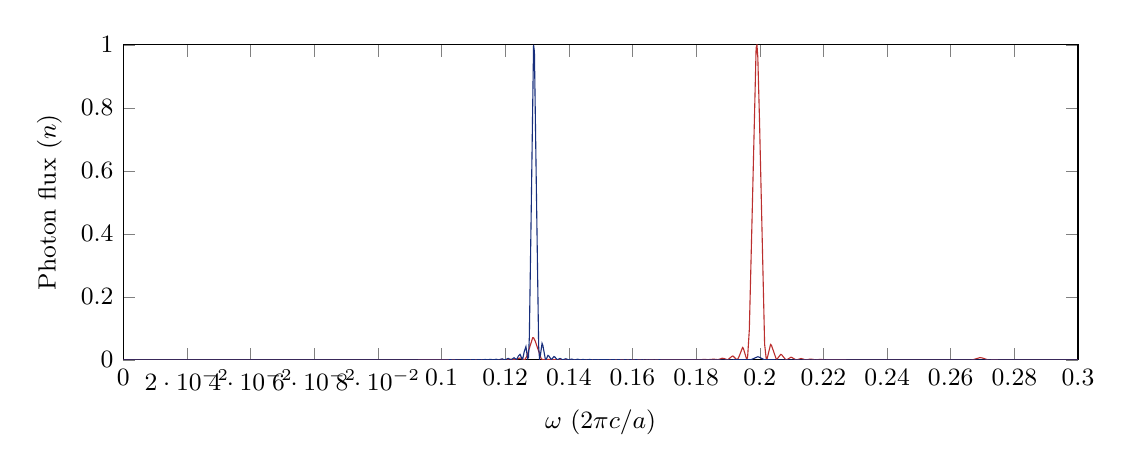
\begin{tikzpicture}

\begin{axis}[%
width=\figW,
height=\figH,
at={(0\figW,0.5\figH)},
scale only axis,
xmin=0,
xmax=0.3,
ymin=0,
ymax=1,
ylabel={Photon flux ($n$)},
xlabel={$\omega$ ($2 \pi c/a$)},
axis background/.style={fill=white}
]
\addplot [color=mode2]
  table[row sep=crcr]{%
0	2.02692564466034e-05\\
0.103292102248673	0.000280380826124693\\
0.107562576760246	0.000190615556102669\\
0.108630195388139	0.00026995448538969\\
0.109697814016032	0.000519930067296892\\
0.111299241957872	0.000215296157155986\\
0.112900669899712	0.000634176485360793\\
0.113968288527605	0.00020327735682879\\
0.115836621126418	0.000942878467160568\\
0.117171144411285	0.000326515510382208\\
0.118772572353125	0.00140039239467527\\
0.120107095637991	0.00035373842841957\\
0.120640904951938	0.00116074002404076\\
0.121441618922858	0.00244261461512596\\
0.122242332893778	0.0013850202900576\\
0.122776142207724	0.000408587791816073\\
0.123309951521671	0.000993757115390403\\
0.124644474806538	0.00579810982243822\\
0.124911379463511	0.00525849068435669\\
0.125978998091404	0.000602444647397116\\
0.126245902748378	0.00183188292919789\\
0.126779712062324	0.0112196277781009\\
0.128648044661137	0.0704843920079685\\
0.128914949318111	0.0701279677450288\\
0.129448758632057	0.0593096830285558\\
0.131317091230871	0.00378945819138909\\
0.131850900544817	0.000631914808392198\\
0.13211780520179	0.000505948784009114\\
0.133185423829684	0.00154458353336451\\
0.13612137505639	0.000304034172873946\\
0.13852351696915	0.000350593787477038\\
0.139591135597043	0.000147372181025895\\
0.141192563538883	0.000559332596227868\\
0.142793991480723	0.000174242982558193\\
0.14412851476559	0.000556450780817563\\
0.145996847364403	0.000234867995221322\\
0.147331370649269	0.00053685754884869\\
0.148932798591109	0.000220053094867056\\
0.150267321875976	0.000575031354170585\\
0.151868749817816	0.000204490570465232\\
0.153203273102682	0.000559917053416736\\
0.155071605701496	0.000241972842460081\\
0.156406128986362	0.000503333759755531\\
0.158007556928202	0.000215640841144671\\
0.159608984870042	0.000468432273565522\\
0.160943508154908	0.000198510235661642\\
0.162278031439775	0.000568700683763135\\
0.163879459381615	0.000186873780516628\\
0.165480887323455	0.000521887940909016\\
0.166815410608321	0.000215236657740814\\
0.168416838550161	0.0005117451543033\\
0.170018266492001	0.000327827659412305\\
0.171352789776868	0.000573903968672962\\
0.172954217718708	0.000366358291039814\\
0.174555645660547	0.000612415457353244\\
0.176157073602387	0.000535231396460611\\
0.179893738800014	0.000796722977213449\\
0.180961357427907	0.000640520416625323\\
0.182562785369747	0.00130448052689025\\
0.183897308654613	0.000778589142653274\\
0.185498736596453	0.0022961112541604\\
0.18683325988132	0.000717084788819378\\
0.187367069195266	0.00226714769104364\\
0.188167783166186	0.00518544185419767\\
0.188701592480133	0.004588007759047\\
0.189769211108026	0.00049136922898918\\
0.190036115765	0.00116294283788032\\
0.190569925078946	0.00558154741010597\\
0.191370639049866	0.0121328790656863\\
0.19163754370684	0.0117059872706191\\
0.192171353020786	0.00638171237143981\\
0.192705162334733	0.000833724042838435\\
0.192972066991706	0.00102874885156701\\
0.193505876305653	0.010927048633822\\
0.194573494933546	0.0392075460899508\\
0.194840399590519	0.0365970710964973\\
0.195908018218413	0.000523095981015853\\
0.196174922875386	0.00960501487696508\\
0.196708732189333	0.0951188568627017\\
0.197509446160252	0.423314770014581\\
0.198843969445119	0.990485168117749\\
0.199110874102092	1\\
0.199377778759066	0.961020912376248\\
0.199911588073012	0.760020992106738\\
0.201513016014852	0.050353278565517\\
0.202046825328799	0.000363268209923717\\
0.202313729985772	0.00430040634764217\\
0.203381348613665	0.0489402815684417\\
0.203648253270639	0.0467393166629728\\
0.205249681212478	0.000153564157706176\\
0.205783490526425	0.00731245491864252\\
0.206584204497345	0.017477998742554\\
0.206851109154318	0.0164576038174333\\
0.208185632439185	0.000176797055538858\\
0.208452537096158	0.000338682134933821\\
0.209787060381025	0.00840029692714084\\
0.210053965037998	0.0076256968243178\\
0.211388488322865	3.05309877179916e-05\\
0.211655392979838	0.000388770979337538\\
0.212989916264705	0.00432350519999902\\
0.213523725578651	0.00271916644939618\\
0.214324439549571	0.00013440060224057\\
0.214858248863518	0.000481469477618512\\
0.215925867491411	0.00258951938434993\\
0.216459676805358	0.00196749403237084\\
0.217527295433251	7.94261203567181e-05\\
0.218328009404171	0.000901339134857571\\
0.219128723375091	0.00155366712176597\\
0.219662532689038	0.00106370195726102\\
0.220463246659957	0.000167831813488117\\
0.221263960630877	0.00042014959947223\\
0.222064674601797	0.000883657179136188\\
0.224466816514557	0.000383177031759274\\
0.22553443514245	0.000457560385735079\\
0.22713586308429	0.000249372568820627\\
0.229004195683103	0.000223745701734224\\
0.266370847659367	9.05383916440794e-05\\
0.266904656973314	0.000557174247925341\\
0.267705370944234	0.0026518422284747\\
0.269039894229101	0.00696769036725153\\
0.269306798886074	0.0071006719864235\\
0.269840608200021	0.00623237800756127\\
0.271708940798834	0.0001630669461965\\
0.27224275011278	7.38143888536769e-05\\
0.273577273397647	0.000644937367476395\\
0.27544560599646	6.39473390915413e-05\\
0.2770470339383	0.00020040586779313\\
0.27864846188014	6.63046866131722e-05\\
0.280516794478953	9.55509025191148e-05\\
0.283185841048686	9.75039627970631e-05\\
0.288257029531179	5.94028880258612e-05\\
0.296264169240379	4.77090192534391e-05\\
0.300000834438005	4.15517847882629e-05\\
};
\addplot [color=mode1]
  table[row sep=crcr]{%
0	2.06393170665287e-06\\
0.101957578963806	0.000160355368395093\\
0.102758292934726	0.000394640117033385\\
0.103559006905646	1.42184153222313e-05\\
0.104626625533539	0.000337256041492262\\
0.105427339504459	4.42557245388109e-05\\
0.106228053475379	0.00050961117456616\\
0.107295672103272	0.000107104910455513\\
0.108096386074192	0.0007081861321796\\
0.109164004702085	0.000123430482289466\\
0.109964718673006	0.000755279969964162\\
0.110765432643925	9.80524098581625e-07\\
0.111833051271819	0.000823007742122073\\
0.112633765242738	4.13321900445407e-05\\
0.113701383870632	0.0012064007916226\\
0.114502097841552	5.56713526180808e-05\\
0.115302811812472	0.00164761357596643\\
0.115569716469445	0.00140055991570009\\
0.116103525783392	8.9182165108781e-05\\
0.116637335097338	0.000799033471166499\\
0.117171144411285	0.00201152434768215\\
0.117704953725231	0.000605233355285062\\
0.117971858382205	1.29486297264503e-05\\
0.118238763039178	0.000395338334635786\\
0.119039477010098	0.00338492021670156\\
0.119840190981018	0.000114749296588057\\
0.120107095637991	0.000725177212089534\\
0.120907809608911	0.00492357216524519\\
0.121708523579831	1.15925391288574e-05\\
0.121975428236805	0.00111471197492641\\
0.122776142207724	0.00675067306027621\\
0.123576856178644	0.00043480759280623\\
0.124110665492591	0.0117182855158933\\
0.124644474806538	0.0175954580703515\\
0.125445188777458	0.000395109982169961\\
0.125978998091404	0.0259693298903021\\
0.126512807405351	0.0423195271822019\\
0.127046616719298	0.00435051494031358\\
0.127313521376271	0.00758492452007831\\
0.127580426033244	0.0700169381062403\\
0.128114235347191	0.428853458885456\\
0.128914949318111	1\\
0.129181853975084	0.978965653730684\\
0.129715663289031	0.600060540093866\\
0.130516377259951	0.042489256760581\\
0.130783281916924	0.00353658621280983\\
0.131050186573897	0.0144415357042833\\
0.131583995887844	0.052381748889758\\
0.131850900544817	0.0454543342138174\\
0.132651614515737	0.000193571093205058\\
0.13291851917271	0.00292130120465184\\
0.133452328486657	0.0141548194756904\\
0.13371923314363	0.0122461041229291\\
0.13451994711455	0.000460051181016885\\
0.13532066108547	0.0107268726981755\\
0.135587565742444	0.00910258049532153\\
0.136388279713364	3.30363866760663e-05\\
0.137188993684283	0.00465783062401037\\
0.137455898341257	0.00378439987225354\\
0.137989707655203	0.000223654181801924\\
0.13852351696915	0.00164475667528485\\
0.139057326283097	0.00372407519795659\\
0.139858040254017	0.00012354369887313\\
0.14092565888191	0.00259793142654874\\
0.14172637285283	6.93578188215582e-05\\
0.141993277509803	0.000296295885228615\\
0.142793991480723	0.00204428857673644\\
0.143594705451643	1.88754072589781e-05\\
0.143861610108616	0.000199485477999195\\
0.144395419422563	0.00129910800239896\\
0.145463038050456	3.4893455505669e-05\\
0.14653065667835	0.00137405419880365\\
0.147331370649269	6.67469440296387e-06\\
0.148398989277163	0.000795328220045688\\
0.149199703248083	3.71591303682806e-05\\
0.150000417219003	0.000897471170834718\\
0.151334940503869	0.000338374715313172\\
0.151868749817816	0.000781321616889263\\
0.152936368445709	6.76187558306118e-05\\
0.153737082416629	0.000657454011505187\\
0.154804701044522	6.70368494035678e-05\\
0.155605415015442	0.00050126531488659\\
0.156406128986362	9.64535975866987e-06\\
0.157740652271229	0.000346079681024403\\
0.158274461585175	4.32532366922977e-06\\
0.159342080213069	0.000360513929722917\\
0.160142794183989	1.30387188232994e-05\\
0.161210412811882	0.000358813123655599\\
0.162011126782802	1.75896139920084e-05\\
0.163078745410695	0.000300704353936698\\
0.163879459381615	2.95506590635153e-05\\
0.164947078009508	0.000262608181982538\\
0.165747791980428	2.75848363189279e-05\\
0.166815410608321	0.000180790797960517\\
0.167616124579241	7.0114675727817e-05\\
0.168416838550161	0.000318008178997964\\
0.169484457178054	5.1387546993853e-05\\
0.170285171148974	0.000228234818772766\\
0.171352789776868	7.09439892521146e-05\\
0.172153503747787	0.000222394462361608\\
0.173221122375681	9.18923666133331e-05\\
0.174288741003574	9.29286526150097e-05\\
0.175356359631467	0.000181701243112897\\
0.191370639049866	0.000184578433084948\\
0.192438257677759	0.000441316747346931\\
0.193505876305653	0.000258316513111367\\
0.195641113561439	0.000914107270121978\\
0.196975636846306	0.000254395875616931\\
0.197509446160252	0.0017247150963462\\
0.199377778759066	0.0100386061881148\\
0.199911588073012	0.00826497169257268\\
0.201246111357879	0.00121397797593681\\
0.201779920671825	0.000387440590282617\\
0.203648253270639	0.000712304747895631\\
0.204982776555505	0.000149381169535001\\
0.224466816514557	3.49675174335928e-05\\
0.22873729102613	5.6534806154529e-05\\
0.233274670194676	7.01903912192492e-06\\
0.237812049363223	4.95226821242145e-05\\
0.242616333188743	1.35944100509988e-05\\
0.247420617014262	1.59989754613399e-05\\
0.260498945205955	9.04671562773629e-07\\
0.270908226827914	0.000207594294210356\\
0.2730434640837	1.56119033378754e-05\\
0.299200120467085	5.11728957763857e-06\\
0.300000834438005	2.7223879450089e-05\\
};
\end{axis}
\end{tikzpicture}%
		\subcaption{RL}
	\end{subfigure}%
	\begin{subfigure}{0.33\textwidth}
		\centering
		% This file was created by matlab2tikz.
%
%The latest updates can be retrieved from
%  http://www.mathworks.com/matlabcentral/fileexchange/22022-matlab2tikz-matlab2tikz
%where you can also make suggestions and rate matlab2tikz.
%
\definecolor{mycolor1}{rgb}{0.00000,0.44700,0.74100}%
\definecolor{mycolor2}{rgb}{0.85000,0.32500,0.09800}%
%
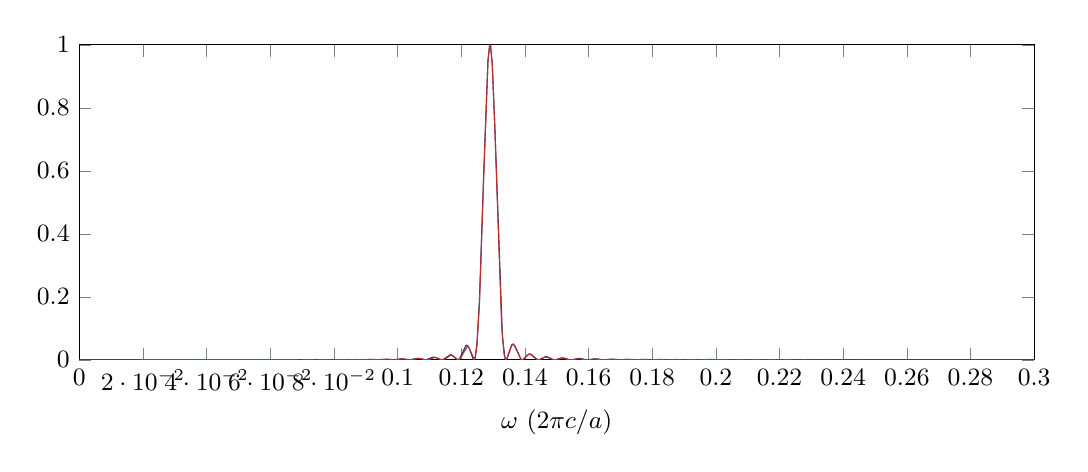
\begin{tikzpicture}

\begin{axis}[%
width=\figW,
height=\figH,
at={(0\figW,0\figH)},
scale only axis,
xmin=0,
xmax=0.3,
ymin=0,
ymax=1,
xlabel={$\omega$ ($2 \pi c/a$)},
axis background/.style={fill=white}
]
\addplot [color=mode1, forget plot]
  table[row sep=crcr]{%
0	3.88673264386519e-05\\
0.0587190245341291	0.000288895213929496\\
0.0605873571329423	0.000407554525789999\\
0.0635233083596487	0.000104902306033106\\
0.0659254502724087	0.000323619183853818\\
0.0683275921851685	6.37155649954035e-05\\
0.0709966387549015	0.000344282085255943\\
0.073131876010688	4.95531779189928e-05\\
0.0760678272373945	0.000488692707976579\\
0.078203064493181	6.99013508840274e-05\\
0.0811390157198875	0.000738307353089551\\
0.083274252975674	6.03439972830522e-05\\
0.0862102042023805	0.000966774114379731\\
0.0886123461151402	0.000110279287079296\\
0.0912813926848735	0.00119415637000886\\
0.09341662994066	4.18238352311029e-05\\
0.0944842485685533	0.000854902627853038\\
0.0955518671964464	0.00179604323857063\\
0.0963525811673664	0.00167486796267857\\
0.0984878184231528	6.88471203496022e-05\\
0.0992885323940729	0.00090853043528738\\
0.100623055678939	0.00288064910562102\\
0.101156864992886	0.00295635254335092\\
0.101690674306833	0.00242743530213541\\
0.103292102248673	6.95029485608956e-05\\
0.104092816219592	0.000754119973114253\\
0.106228053475379	0.00504008049988403\\
0.106761862789326	0.00432803203342691\\
0.108630195388139	0.000105426192973379\\
0.109164004702085	0.000947613905575073\\
0.109964718673006	0.00428541423423412\\
0.111032337300899	0.00845278913092984\\
0.111299241957872	0.00869319375076816\\
0.111566146614845	0.00848371994951602\\
0.112099955928792	0.00679729066571122\\
0.113701383870632	0.000108503225145329\\
0.113968288527605	0.000341980879380976\\
0.114502097841552	0.00270341483409275\\
0.116637335097338	0.01667844870554\\
0.117171144411285	0.0140440989154202\\
0.118772572353125	0.000136660284805856\\
0.119039477010098	0.000410371616097471\\
0.119573286324045	0.00544565689993037\\
0.120374000294965	0.0226680807617432\\
0.121441618922858	0.0451273515122541\\
0.121708523579831	0.0467140129595078\\
0.121975428236805	0.0458105064198076\\
0.122509237550751	0.0364590241432714\\
0.123843760835618	0.000345257283584921\\
0.124110665492591	0.00130793613966573\\
0.124377570149564	0.00885492636316787\\
0.124911379463511	0.0497441765140558\\
0.125712093434431	0.18913220418551\\
0.127046616719298	0.592313419780696\\
0.128381140004164	0.949979994686141\\
0.128914949318111	1\\
0.129181853975084	0.998233506489319\\
0.129715663289031	0.941449581289506\\
0.130516377259951	0.746188777188888\\
0.13291851917271	0.0746684419354082\\
0.13371923314363	0.00562021939329149\\
0.133986137800604	0.000309725835684782\\
0.134253042457577	0.00130392986105687\\
0.134786851771524	0.0151237426976352\\
0.135854470399417	0.0469962225820375\\
0.136388279713364	0.0500184016206293\\
0.13692208902731	0.0428974276549838\\
0.138790421626123	0.00144772637971657\\
0.139057326283097	0.000113224222431541\\
0.13932423094007	0.000352800415001298\\
0.139858040254017	0.00448413965679317\\
0.141192563538883	0.0180653974582243\\
0.141459468195857	0.0187222731595087\\
0.14172637285283	0.0183715240512414\\
0.142260182166776	0.015036217094748\\
0.143861610108616	0.000765594181906692\\
0.144395419422563	0.000160780041085884\\
0.14492922873651	0.00213476037770843\\
0.14653065667835	0.0101519854944379\\
0.147064465992296	0.00961123495512806\\
0.147865179963216	0.00574264264904767\\
0.148932798591109	0.000579080469022886\\
0.149466607905056	9.20797609047508e-05\\
0.150000417219003	0.00119982075952163\\
0.151601845160843	0.00650647183236952\\
0.152135654474789	0.00636520457224066\\
0.152936368445709	0.00403646604253405\\
0.154003987073602	0.000519664576796641\\
0.154537796387549	5.82388821335211e-05\\
0.155071605701496	0.000699153823800369\\
0.156939938300309	0.00464667197681123\\
0.157740652271229	0.00371623167266999\\
0.159342080213069	0.000174740337848256\\
0.159875889527015	0.000137813505997508\\
0.160676603497935	0.0013459868674961\\
0.161744222125828	0.00320381554906368\\
0.162278031439775	0.00335056467496297\\
0.162811840753722	0.00283162744897725\\
0.164680173352535	6.19170065134789e-05\\
0.165480887323455	0.000530729543030128\\
0.167082315265295	0.00247776964275337\\
0.167883029236215	0.00217635061654464\\
0.170018266492001	8.11407369474271e-05\\
0.170818980462921	0.000654598787708238\\
0.172153503747787	0.00189503778019473\\
0.172954217718708	0.00171486090331996\\
0.175089454974494	0.000104864785164915\\
0.176157073602387	0.000777714138052499\\
0.17722469223028	0.00153065072087433\\
0.178292310858174	0.00123067644327723\\
0.179893738800014	0.00013470216006839\\
0.180961357427907	0.000480879325755801\\
0.182562785369747	0.00134901621616046\\
0.18363040399764	0.000904366759798103\\
0.184964927282507	0.000165559268547444\\
0.1860325459104	0.000455645715565334\\
0.18763397385224	0.00121609538014744\\
0.188701592480133	0.000845320344863287\\
0.190036115765	0.000194768298143577\\
0.191103734392893	0.000438096030068946\\
0.192705162334733	0.00111986859121838\\
0.194039685619599	0.000631420797184035\\
0.195374208904466	0.000163279525361881\\
0.196708732189333	0.00077908796899373\\
0.198043255474199	0.0014169294652675\\
0.199377778759066	0.0010723485577786\\
0.200979206700906	0.000595942279109973\\
0.203915157927612	0.000620747971421531\\
0.205783490526425	0.000241965638161146\\
0.208719441753132	0.000643475537537297\\
0.210854679008918	0.00018060762274219\\
0.214057534892598	0.000513309625902902\\
0.215925867491411	0.000148477917433665\\
0.219128723375091	0.000465484630120638\\
0.221263960630877	0.000149010222779467\\
0.22393300720061	0.000476953999740459\\
0.22633514911337	0.000116826618160815\\
0.229271100340077	0.000380836597472234\\
0.231406337595863	8.5974455506399e-05\\
0.23434228882257	0.000345126849571109\\
0.23674443073533	9.30502235432229e-05\\
0.239413477305063	0.000315249265120388\\
0.241815619217822	7.2753509476664e-05\\
0.244484665787556	0.000292138733504865\\
0.247153712357289	9.32220429585851e-05\\
0.249555854270049	0.000273054242184045\\
0.252224900839782	7.76272988718407e-05\\
0.254893947409515	0.000219004705521719\\
0.257296089322275	6.44965757119476e-05\\
0.259965135892008	0.000202992908045152\\
0.262634182461741	8.58989335559279e-05\\
0.265036324374501	0.000188453043735048\\
0.267705370944234	7.55468344884047e-05\\
0.270374417513967	0.000140967971464789\\
0.272776559426727	7.74017951870043e-05\\
0.27544560599646	0.000143621887806145\\
0.278114652566193	0.000104671046546656\\
0.280783699135926	0.000115930333205894\\
0.283185841048686	9.9361801052078e-05\\
0.285854887618419	0.000115845411306381\\
0.288523934188152	0.000116789163551401\\
0.291192980757886	8.36957315482056e-05\\
0.293862027327619	0.000128088581529351\\
0.296531073897352	5.52903256878512e-05\\
0.299467025124058	0.000150828081684651\\
0.300000834438005	0.00015982821120919\\
};
\addplot [color=mode2, forget plot]
  table[row sep=crcr]{%
0	0.000134350006603778\\
0.0659254502724087	0.000546352358206104\\
0.0672599735572752	0.000460862662837735\\
0.0691283061560883	9.55790606635976e-05\\
0.0720642573827948	0.000672134212729381\\
0.0741994946385813	8.7401919838026e-05\\
0.0771354458652878	0.00075397678012834\\
0.0792706831210743	7.01283008002207e-05\\
0.0819397296908073	0.000925324458987964\\
0.0843418716035673	0.000102239839298246\\
0.0870109181733003	0.00115823206292909\\
0.0891461554290869	7.49940352624545e-05\\
0.089946869400007	0.000622957480105324\\
0.0912813926848735	0.0017744005502347\\
0.0920821066557933	0.00160304945766754\\
0.0942173439115799	0.000121089660574336\\
0.0950180578824997	0.000899620005289536\\
0.0963525811673664	0.0024763252773865\\
0.0971532951382863	0.00221721635786709\\
0.0990216277370994	6.88004995530456e-05\\
0.0998223417080195	0.00073837292708534\\
0.101423769649859	0.00335373569011055\\
0.102224483620779	0.00297396420774598\\
0.104092816219592	3.92697161286648e-05\\
0.104626625533539	0.000500658243272945\\
0.105694244161432	0.00319538613993675\\
0.106494958132352	0.00467040498185978\\
0.107028767446299	0.00449833231831542\\
0.107829481417219	0.00259624950391957\\
0.108897100045112	7.86111653929833e-05\\
0.109430909359059	0.000310584416365334\\
0.109964718673006	0.00180181468622176\\
0.111566146614845	0.00739135487676301\\
0.112099955928792	0.00694240725090878\\
0.112900669899712	0.0037230043267944\\
0.113701383870632	0.000412414406023132\\
0.113968288527605	1.85220806636632e-05\\
0.114235193184578	0.000176071948576606\\
0.114769002498525	0.00225987597121224\\
0.116637335097338	0.0147183810942626\\
0.116904239754312	0.0145579495701427\\
0.117438049068258	0.0118070136074451\\
0.119039477010098	2.465222358361e-05\\
0.119306381667071	0.000947501410340168\\
0.119840190981018	0.00718090974939378\\
0.121975428236805	0.0438753132707257\\
0.122509237550751	0.0364499498612483\\
0.124110665492591	0.000622739923811677\\
0.124377570149564	0.00675661841620934\\
0.124911379463511	0.0442116066621001\\
0.125712093434431	0.178829630884551\\
0.127046616719298	0.581835543870001\\
0.128381140004164	0.947534486194421\\
0.128914949318111	1\\
0.129181853975084	0.998877675699094\\
0.129715663289031	0.942079961332503\\
0.130516377259951	0.744211160416836\\
0.132651614515737	0.11315772679601\\
0.133452328486657	0.0164085403245755\\
0.133986137800604	7.10423854644038e-05\\
0.134253042457577	0.00195643439784354\\
0.135053756428497	0.0262844492153576\\
0.135854470399417	0.0474938857403329\\
0.13612137505639	0.0496993558829111\\
0.136388279713364	0.0491230041958695\\
0.13692208902731	0.0408526036414969\\
0.138790421626123	0.000795706382213268\\
0.139057326283097	5.41550979704652e-06\\
0.13932423094007	0.000710933427661375\\
0.14012494491099	0.00851816587544341\\
0.14092565888191	0.0164739381569738\\
0.141459468195857	0.0178341636514858\\
0.141993277509803	0.0154444100365945\\
0.143861610108616	0.000286117622562365\\
0.14412851476559	1.36753117139232e-05\\
0.144395419422563	0.000408616499049996\\
0.145196133393483	0.00428969739499285\\
0.146263752021376	0.00902659670834471\\
0.14653065667835	0.00917987763214145\\
0.147064465992296	0.00804337300542679\\
0.149199703248083	1.9707078568576e-05\\
0.149733512562029	0.000845586908188922\\
0.151334940503869	0.00541018781790625\\
0.151868749817816	0.00530878162286963\\
0.152669463788736	0.00332930208959281\\
0.153737082416629	0.000382642886062268\\
0.154270891730576	2.91624250183808e-05\\
0.154804701044522	0.00058806056570293\\
0.156406128986362	0.00353191533932695\\
0.157206842957282	0.00313738891295468\\
0.159342080213069	5.36897724505714e-05\\
0.159875889527015	0.000466589778830073\\
0.161477317468855	0.00245063100627285\\
0.162278031439775	0.00213316748429437\\
0.164146364038588	6.73618161206591e-05\\
0.164947078009508	0.000415498892222477\\
0.166548505951348	0.00180231145694543\\
0.167349219922268	0.00151769174651983\\
0.169217552521081	8.40223087013037e-05\\
0.170285171148974	0.000626232967441132\\
0.171619694433841	0.00141558579819789\\
0.172687313061734	0.000945225650540671\\
0.174021836346601	0.000114312445260945\\
0.175089454974494	0.00041344848499425\\
0.176690882916334	0.00116429745160396\\
0.178025406201201	0.000549959079481965\\
0.179093024829094	9.4587078521613e-05\\
0.180160643456987	0.000403374882612662\\
0.181762071398827	0.000995137993678785\\
0.183363499340667	0.000299459587668416\\
0.18443111796856	0.000105410871372502\\
0.187367069195266	0.000746947820029709\\
0.189502306451053	0.000103043392124524\\
0.192438257677759	0.000689519088927781\\
0.194573494933546	8.11926997945633e-05\\
0.198043255474199	0.000898373506712069\\
0.200178492729986	0.000580536876829685\\
0.202313729985772	0.000510478358584754\\
0.204448967241559	0.000109648218290737\\
0.207918727782212	0.000336144282479856\\
0.209787060381025	0.000151452203610569\\
0.212456106950758	0.000387339872801595\\
0.214858248863518	0.000162692367967177\\
0.217527295433251	0.000333407369542016\\
0.219929437346011	0.000153228801843541\\
0.222331579258771	0.000331965315724325\\
0.225000625828504	0.000129305397597923\\
0.227402767741264	0.000293873253189636\\
0.230071814310997	0.000105626887377586\\
0.23274086088073	0.000218607833060824\\
0.23514300279349	9.1631430102268e-05\\
0.237812049363223	0.000184056413309541\\
0.240214191275983	8.76970342735817e-05\\
0.242883237845716	0.000156349295140634\\
0.245552284415449	0.000117946598475971\\
0.247954426328209	0.000136546725246101\\
0.250623472897942	0.000117511195575792\\
0.253292519467675	9.42269177877098e-05\\
0.255961566037408	0.000139284877229029\\
0.258630612607141	5.98940084699517e-05\\
0.261566563833848	0.000163126341109265\\
0.27864846188014	4.33498806224897e-05\\
0.285321078304473	4.38910115891922e-05\\
0.291459885414859	9.86946118051169e-05\\
0.300000834438005	2.33733493741894e-05\\
};
\end{axis}
\end{tikzpicture}%
		\subcaption{LR}
	\end{subfigure}%
	\begin{subfigure}{0.33\textwidth}
		\centering
		% This file was created by matlab2tikz.
%
%The latest updates can be retrieved from
%  http://www.mathworks.com/matlabcentral/fileexchange/22022-matlab2tikz-matlab2tikz
%where you can also make suggestions and rate matlab2tikz.
%
\definecolor{mycolor1}{rgb}{0.00000,0.44700,0.74100}%
\definecolor{mycolor2}{rgb}{0.85000,0.32500,0.09800}%
%
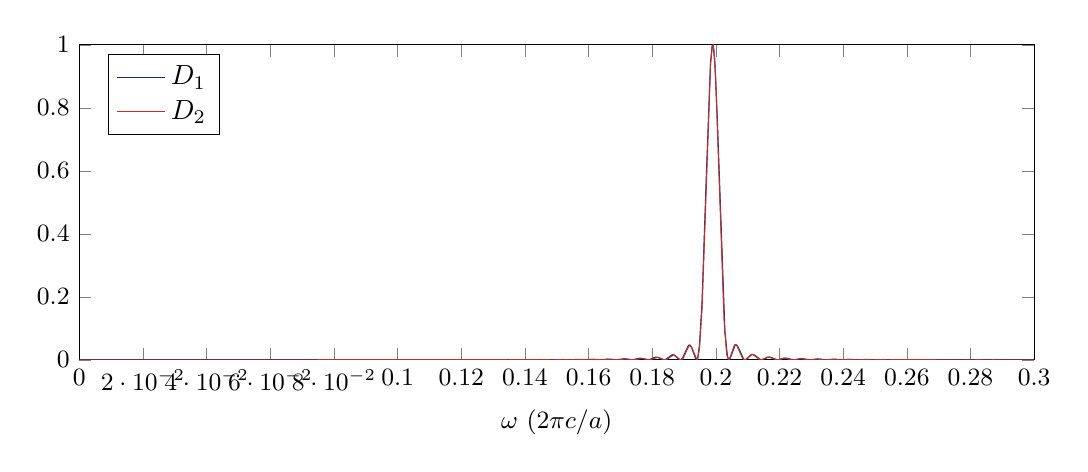
\begin{tikzpicture}

\begin{axis}[%
width=\figW,
height=\figH,
at={(0\figW,0\figH)},
scale only axis,
xmin=0,
xmax=0.3,
ymin=0,
ymax=1,
xlabel={$\omega$ ($2 \pi c/a$)},
axis background/.style={fill=white},
legend pos=north west
]
\addplot [color=mode1]
  table[row sep=crcr]{%
0	1.55493558309239e-05\\
0.128648044661137	0.000291401836858496\\
0.130783281916924	0.000272579306686227\\
0.133185423829684	0.000132906235705388\\
0.135854470399417	0.000282632640331348\\
0.137989707655203	0.000107228709113727\\
0.14092565888191	0.000354175823229053\\
0.143060896137696	0.000107132078084549\\
0.145729942707429	0.000529848463097338\\
0.148132084620189	0.00011034827748313\\
0.150801131189922	0.000676029799295597\\
0.153203273102682	8.6709076011271e-05\\
0.155872319672415	0.000725615531831814\\
0.158007556928202	6.95901860032766e-05\\
0.159342080213069	0.000872165130341385\\
0.160409698840962	0.00136635364920878\\
0.161477317468855	0.000885334125582116\\
0.162811840753722	5.24261914098823e-05\\
0.163612554724642	0.000370662827645418\\
0.165747791980428	0.00213950279486941\\
0.166548505951348	0.00151524255748625\\
0.167883029236215	9.99298748551869e-05\\
0.168683743207134	0.000451329014977686\\
0.171085885119894	0.00343490754811349\\
0.171886599090814	0.00224906255381763\\
0.172954217718708	0.000302554660580823\\
0.173488027032654	0.00017879873144433\\
0.174021836346601	0.000919156488057515\\
0.176157073602387	0.00543332780202976\\
0.176690882916334	0.00464728239889034\\
0.178559215515147	0.000121828812656988\\
0.179093024829094	0.000933252851363031\\
0.179893738800014	0.00425022274790998\\
0.180961357427907	0.00837555305559978\\
0.18122826208488	0.00860274235849001\\
0.181495166741854	0.00838172254753555\\
0.1820289760558	0.00668435077258689\\
0.18363040399764	9.27083512791693e-05\\
0.183897308654613	0.000346171492089375\\
0.18443111796856	0.00272661757263548\\
0.186299450567373	0.016515440220733\\
0.18683325988132	0.0155673636769622\\
0.18763397385224	0.00861458379711411\\
0.18843468782316	0.00110254813881161\\
0.188701592480133	0.000130329011890584\\
0.188968497137106	0.000447910380210859\\
0.189502306451053	0.00555166721986233\\
0.190303020421973	0.0228470182196445\\
0.191370639049866	0.0455482939349976\\
0.19163754370684	0.0472468463701474\\
0.191904448363813	0.0464698105071626\\
0.192438257677759	0.0373595815668704\\
0.193772780962626	0.000582682443470706\\
0.194039685619599	0.000953620516230158\\
0.194306590276573	0.00770275184263558\\
0.194840399590519	0.0463805201203464\\
0.195641113561439	0.181350090175954\\
0.196975636846306	0.5789769997712\\
0.198310160131172	0.942252496575551\\
0.198843969445119	0.99825962608984\\
0.199110874102092	1\\
0.199644683416039	0.950558949856845\\
0.200445397386959	0.764740867950573\\
0.202847539299719	0.0874677020756052\\
0.203648253270639	0.00940986069280059\\
0.204182062584585	0.000290886130887014\\
0.204715871898532	0.0111964738588415\\
0.206050395183399	0.0469218182207407\\
0.206317299840372	0.0480789686741683\\
0.206584204497345	0.0466769059702812\\
0.207118013811292	0.0376257976481291\\
0.208719441753132	0.00250926353509517\\
0.209253251067078	6.69887869633179e-05\\
0.209520155724052	0.000969587975592434\\
0.210320869694971	0.00864972503415906\\
0.211121583665892	0.0160331112409842\\
0.211655392979838	0.017175408231457\\
0.212189202293785	0.0148192128118578\\
0.214057534892598	0.000333467470762461\\
0.214324439549571	4.02818042173347e-05\\
0.214591344206545	0.000380854134824471\\
0.215125153520491	0.00253402178169493\\
0.216459676805358	0.00876959050175152\\
0.216726581462331	0.00900869958947359\\
0.216993486119304	0.00877051552680541\\
0.217527295433251	0.00705748228004466\\
0.219128723375091	0.000272039889200215\\
0.219662532689038	0.000179347459904555\\
0.220196342002984	0.00137371627138227\\
0.221530865287851	0.00534614050185867\\
0.222064674601797	0.00552290605915928\\
0.222598483915744	0.0045960448969713\\
0.224466816514557	4.79648292748269e-05\\
0.225267530485477	0.000821715458200867\\
0.226868958427317	0.00380924974414776\\
0.227669672398237	0.00328263718586364\\
0.22953800499705	5.92327265036552e-05\\
0.23033871896797	0.000517587296184674\\
0.23194014690981	0.00275334142803629\\
0.23274086088073	0.0024778958078675\\
0.234876098136516	3.92773102042554e-05\\
0.23594371676441	0.0009665185658283\\
0.237011335392303	0.00207579350585685\\
0.237812049363223	0.00194892818245229\\
0.240214191275983	8.43691858622986e-05\\
0.241281809903876	0.000969422628691374\\
0.242349428531769	0.00168286048158128\\
0.243417047159662	0.00117788989713086\\
0.244751570444529	8.9212386712445e-05\\
0.245819189072422	0.00030498939111645\\
0.247687521671236	0.00135155492492922\\
0.248755140299129	0.000797963957217762\\
0.250089663583995	3.6908011647574e-05\\
0.251157282211889	0.000367919546328865\\
0.252758710153729	0.00110230415849455\\
0.254093233438595	0.0005246527385665\\
0.255427756723462	3.20985488073688e-05\\
0.257029184665301	0.000686157614896654\\
0.258096803293195	0.000878742506423391\\
0.261299659176875	0.000213993016872305\\
0.263167991775688	0.000724239501030954\\
0.266103943002394	0.000184181060117083\\
0.268506084915154	0.000967059785361934\\
0.271975845455807	0.000219003733829215\\
0.27384417805462	0.000384297727108684\\
0.276513224624353	8.83362682626565e-05\\
0.278915366537113	0.000338967445775884\\
0.281584413106846	8.81737632429935e-05\\
0.283986555019606	0.000312097828071956\\
0.286655601589339	8.86890943270213e-05\\
0.289057743502099	0.000300067701469731\\
0.291726790071832	8.27004019099409e-05\\
0.294395836641566	0.000256229286488718\\
0.296797978554325	7.07704273552601e-05\\
0.299467025124058	0.000251704428123389\\
0.300000834438005	0.000162100326521086\\
};
\addlegendentry{$D_1$};
\addplot [color=mode2]
  table[row sep=crcr]{%
0	6.28028652625012e-05\\
0.129982567946004	0.000394692742722524\\
0.131583995887844	0.000698770716094366\\
0.134786851771524	0.00019868256087352\\
0.136655184370337	0.000666974065289372\\
0.139858040254017	0.000256735068325575\\
0.14172637285283	0.000756975321301256\\
0.144662324079536	0.000212968754511822\\
0.14653065667835	0.000885190533250979\\
0.148132084620189	0.000221472399044798\\
0.149199703248083	8.65124002005224e-05\\
0.151868749817816	0.00115568318147807\\
0.154270891730576	0.000157772642941367\\
0.155338510358469	0.00101554189682829\\
0.156406128986362	0.00173331044670522\\
0.157206842957282	0.00147117562233334\\
0.159075175556095	6.96388803462789e-05\\
0.159875889527015	0.000516739486775775\\
0.161477317468855	0.00201506871342882\\
0.162278031439775	0.00171224416975724\\
0.164146364038588	5.78575439533768e-05\\
0.164947078009508	0.000655860005683184\\
0.166548505951348	0.00252726291218996\\
0.167349219922268	0.00210893713455218\\
0.169217552521081	4.73513166596717e-05\\
0.169751361835028	0.000455705499391668\\
0.171619694433841	0.0031529830570276\\
0.172420408404761	0.00251171360091851\\
0.174021836346601	1.91378927785202e-05\\
0.174822550317521	0.000780425841003352\\
0.176690882916334	0.0043952872615558\\
0.17722469223028	0.00384278328508025\\
0.179093024829094	2.19478635807846e-05\\
0.17962683414304	0.000873347255885726\\
0.180694452770934	0.00521815762812161\\
0.181495166741854	0.00752277729454254\\
0.1820289760558	0.00717645931652644\\
0.18282969002672	0.00398844381761898\\
0.183897308654613	4.25200507609969e-05\\
0.18443111796856	0.000826541263138969\\
0.184964927282507	0.00396170238662585\\
0.186566355224347	0.0154554640332349\\
0.187100164538293	0.0146102331768789\\
0.187900878509213	0.00786768019001527\\
0.188701592480133	0.000765609664994615\\
0.188968497137106	1.00751503933072e-05\\
0.18923540179408	0.000583158450087495\\
0.189769211108026	0.0062465476170126\\
0.19083682973592	0.0307335311685133\\
0.19163754370684	0.044838626116368\\
0.191904448363813	0.0455642956425175\\
0.192171353020786	0.0437085502056458\\
0.192705162334733	0.0326095155633743\\
0.194039685619599	8.29826755261998e-05\\
0.194306590276573	0.00426705372360048\\
0.194840399590519	0.0368891203464228\\
0.195641113561439	0.163536508091964\\
0.196708732189333	0.470279547957771\\
0.198310160131172	0.936783366445699\\
0.198843969445119	0.997055164766234\\
0.199110874102092	1\\
0.199377778759066	0.984354536839983\\
0.199911588073012	0.9008230433819\\
0.200979206700906	0.587712085592871\\
0.202580634642745	0.123557976784367\\
0.203381348613665	0.0201415548995225\\
0.203915157927612	0.000406488651291115\\
0.204182062584585	0.00108835887659708\\
0.204715871898532	0.0145567313328479\\
0.205783490526425	0.0458145556500049\\
0.206050395183399	0.0485122389622314\\
0.206584204497345	0.0458241697346764\\
0.207384918468265	0.0276969588192231\\
0.208452537096158	0.00373766110674989\\
0.208986346410105	2.24533793631299e-05\\
0.209253251067078	0.000486565351071278\\
0.209787060381025	0.00475962450493927\\
0.211121583665892	0.0170058642777724\\
0.211388488322865	0.0173118308292897\\
0.211655392979838	0.0166691715286995\\
0.212189202293785	0.013045117629338\\
0.213790630235625	0.000327698357917239\\
0.214057534892598	1.6912870248742e-06\\
0.214324439549571	0.000333045662057163\\
0.214858248863518	0.00251401078911795\\
0.216192772148385	0.00868642775459749\\
0.216459676805358	0.00885659243967174\\
0.216993486119304	0.00778433919550259\\
0.219128723375091	1.08968142209509e-05\\
0.219662532689038	0.000835543978102926\\
0.221263960630877	0.00529807561889384\\
0.221797769944824	0.00516775764115707\\
0.222598483915744	0.003184733474213\\
0.223666102543637	0.000317415799661047\\
0.224199911857584	2.24659696721474e-05\\
0.224733721171531	0.000632607768083604\\
0.22633514911337	0.00357108285710717\\
0.22713586308429	0.00310004865283231\\
0.229004195683103	1.9159038553207e-05\\
0.229804909654023	0.000509891041929667\\
0.231406337595863	0.00256350123591442\\
0.232207051566783	0.00217146493457077\\
0.234075384165596	8.57470921800108e-06\\
0.234876098136516	0.000433689156983164\\
0.236477526078356	0.0019350223537693\\
0.237278240049276	0.00159491485970564\\
0.239146572648089	7.41945127402666e-06\\
0.240214191275983	0.000620431913449071\\
0.241548714560849	0.00151250505035638\\
0.242616333188743	0.00099358717544229\\
0.243950856473609	3.53715982044367e-05\\
0.245018475101502	0.000335135952300725\\
0.246619903043342	0.00120572852227885\\
0.247687521671236	0.000760124777400062\\
0.249022044956102	2.13407546516553e-05\\
0.250089663583995	0.000296490869482025\\
0.251691091525835	0.000967715917518985\\
0.253025614810702	0.000422026775932727\\
0.254093233438595	1.05853251659571e-05\\
0.255427756723462	0.000402060862756404\\
0.256762280008328	0.000786201423783384\\
0.260232040548981	0.000274503218366862\\
0.261833468490821	0.000689916951627456\\
0.265036324374501	0.00023287435433339\\
0.266904656973314	0.000956960594683309\\
0.268239180258181	0.000576948236111097\\
0.269840608200021	8.73507236096582e-05\\
0.278114652566193	0.000142858287752068\\
0.279982985165006	0.000112473223961018\\
0.282118222420793	0.000326971236328966\\
0.285054173647499	0.000110449333495799\\
0.287189410903286	0.000291454661272006\\
0.290125362129992	0.000100987672789321\\
0.292527504042752	0.000210638371687333\\
0.294929645955512	6.09022446864671e-05\\
0.297598692525245	0.000172780313424825\\
0.300000834438005	6.53213967842792e-05\\
};
\addlegendentry{$D_2$};
\end{axis}
\end{tikzpicture}%
		\subcaption{TR}
	\end{subfigure}
	\caption[Fourier components of the optical AB effect]{Frequencies of the optical Aharonov-Bohm effect for detector $D_1$ at $1.5 \mu m$ and detector $D_2$ at $58 \mu m$ for \textbf{(a)} left to right \textbf{(b)} right to left, and \textbf{(c)} time-reversed directions. Note that for all graphs, both $D_1$ and $D_2$ are shown, however there is an overlap in the LR and TR paths.}
	\label{fig:final}
\end{figure}


\begin{table}[b]
	\centering
	\begin{tabular}{|l|l|l|}
		\hline
		Direction & Input         & Output         \\
		\hline
		Left to right (LR) & $\ket{1}$  & $\ket{2}$  \\
		Right to left (RL) & $\bra{1}$ & $\bra{1}$ \\
		Time-reversed (TR) & $\bra{2}$ & $\bra{2}$ \\
		\hline
	\end{tabular}
	\caption[Summary of mode transitions in the photonic AB effect.]{Summary of mode transitions in the photonic AB effect.}
	\label{tab:modess}
\end{table}

 
    %\chapter{A photonic Aharonov-Bohm effect}

\section{Mach-Zehnder interferometer}

\section{Reduction of device complexity}
To demonstrate non-reciprocal propagation we simulate the structure of figure 
\begin{figure}[t]
\centering
\setlength{\figH}{1\textwidth}
\setlength{\figW}{1\textwidth}

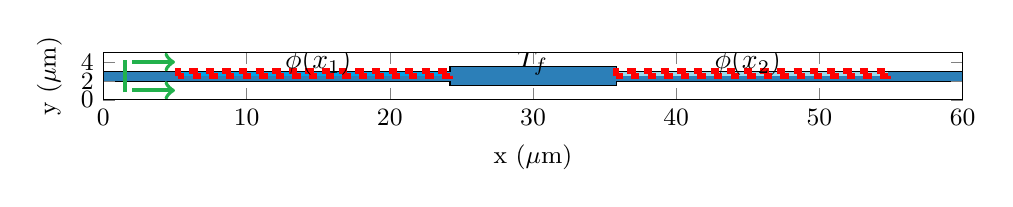
\begin{tikzpicture}
    \begin{axis}[%
width=0.9\figW,
height=0.15\figH,
at={(0\figW,0\figH)},
scale only axis,
axis on top,
xmin=0,
xmax=60,
xlabel={$\text{x (}\mu\text{m)}$},
ymin=0,
ymax=5,
ylabel={$\text{y (}\mu\text{m)}$},
axis background/.style={fill=white},
]
\fill[fill=eps] (0,1.95) rectangle (60,3.05);
\fill[fill=eps] (24.2,1.5) rectangle (35.8,3.5);
\fill[fill=modup] (5.2,2.5) rectangle (24.2,3.05);
\fill[fill=moddown] (35.8,2.5) rectangle (54.8,3.05);
\draw (0,1.95) -- (24.2,1.95) -- (24.2,1.5) -- (35.8,1.5) -- (35.8,1.95) -- (60,1.95);
\draw (0,3.05) -- (24.2,3.05) -- (24.2,3.5) -- (35.8,3.5) -- (35.8,3.05) -- (60,3.05);
\draw[draw=src, line width=0.5mm] (1.5,0.8) -- (1.5,4.2);
\draw[line width=0.5mm, draw=src, ->] (2,4) -- (5,4);
\draw[line width=0.5mm, draw=src, ->] (2,1) -- (5,1);
\draw[dashed, draw=red, line width=0.7mm] (5.2,2.5) -- (5.2,3.05) -- (24.2,3.05) -- (24.2,2.5) -- (5.2,2.5);
\draw[dashed, draw=red, line width=0.7mm] (35.8,2.5) -- (35.8,3.05) -- (54.8,3.05) -- (54.8,2.5) -- (35.8,2.5);
\node at (15,4) {$\phi(x_1)$};
\node at (45,4) {$\phi(x_2)$};
\node at (30,4) {$T_f$};
\end{axis}
\end{tikzpicture}
\caption[The modulated waveguide structure]{The modulated waveguide structure. The dark blue region is a material of unity permeability and permittivity of $\epsilon_{wg} = 12.25$. The light blue sections are regions where the permittivity is modulated by an amount $0.1 \epsilon_{wg} \cos(\omega t + \phi)$, with $\phi=0$ on the left and $\phi=\frac{\pi}{2}$ on the right. The modulation region is chosen to only cover the upper half of the waveguide to maximise the coupling. The diagonal lines around the edges represent the \textit{PML} layer, marking the point where the fields effectively decay to zero. Note that the layer width is constant across the \textit{x} and \textit{y} directions. The red line indicates the region over which the modal source is injected, in this case, from left to right (LR).}
\label{fig:cavity}
\end{figure}


                    
\begin{figure}[t]
    \centering
    \setlength{\figH}{1\textwidth}
	\setlength{\figW}{1\textwidth}
	% This file was created by matlab2tikz.
%
%The latest updates can be retrieved from
%  http://www.mathworks.com/matlabcentral/fileexchange/22022-matlab2tikz-matlab2tikz
%where you can also make suggestions and rate matlab2tikz.
%
\pgfplotsset{fangFields/.style={
	width=0.8\figW,
height=0.08\figH,
	scale only axis,
	axis on top,
	title style = {at={(0.4\figH,0.06\figH)}},
	xmin=0,
	xmax=60,
	ymin=0,
	clip=false,
	ymax=5,
	axis background/.style={fill=white},
	colormap={mymap}{[1pt] rgb(0pt)=(0,0,1); rgb(31pt)=(1,1,1); rgb(32pt)=(1,1,1); rgb(63pt)=(1,0,0)},
	colorbar,
	colorbar style={width=.01\linewidth, at={(1.02,0.04\figH)}, anchor=east}	
	}
}

\begin{tikzpicture}
\begin{axis}[%
fangFields,
at={(0\figW,0.95\figH)},
title = {Total field},
point meta min=-23,
point meta max=23,
xticklabels={,,},
colorbar style={title={$V / \mu m$}, width=.01\linewidth, at={(1.02,0.04\figH)}, anchor=east},
ylabel={$\text{y (}\mu\text{m)}$}
]
\addplot [forget plot] graphics [xmin=0, xmax=60, ymin=0, ymax=5] {graphs/fangcavity/LR/totalfield.png};
\draw (0,1.95) -- (24.2,1.95) -- (24.2,1.5) -- (35.8,1.5) -- (35.8,1.95) -- (60,1.95);
\draw (0,3.05) -- (24.2,3.05) -- (24.2,3.5) -- (35.8,3.5) -- (35.8,3.05) -- (60,3.05);
\node at (55,6) {$\longrightarrow \ket{2}$};
\node at (5,6) {$\ket{1} \longrightarrow$};
\node at (-2,7) {\textbf{(a)}};
\end{axis}

\begin{axis}[%
fangFields,
at={(0\figW,0.8\figH)},
title = {$\omega_1 - \Omega$},
point meta min=-0.11845616858408,
point meta max=0.11845616858408,
xticklabels={,,},
ylabel={$\text{y (}\mu\text{m)}$}
]
\addplot [forget plot] graphics [xmin=0, xmax=60, ymin=0, ymax=5] {graphs/fangcavity/LR/nameoffile2-1.png};
\draw (0,1.95) -- (24.2,1.95) -- (24.2,1.5) -- (35.8,1.5) -- (35.8,1.95) -- (60,1.95);
\draw (0,3.05) -- (24.2,3.05) -- (24.2,3.5) -- (35.8,3.5) -- (35.8,3.05) -- (60,3.05);
\end{axis}

\begin{axis}[%
fangFields,
at={(0\figW,0.65\figH)},
title = {$\omega_1$},
point meta min=-6.64719566790506,
point meta max=6.64719566790506,
xticklabels={,,},
ylabel={$\text{y (}\mu\text{m)}$}
]
\addplot [forget plot] graphics [xmin=0, xmax=60, ymin=0, ymax=5] {graphs/fangcavity/LR/nameoffile2-2.png};
\draw (0,1.95) -- (24.2,1.95) -- (24.2,1.5) -- (35.8,1.5) -- (35.8,1.95) -- (60,1.95);
\draw (0,3.05) -- (24.2,3.05) -- (24.2,3.5) -- (35.8,3.5) -- (35.8,3.05) -- (60,3.05);
\end{axis}

\begin{axis}[%
fangFields,
at={(0\figW,0.5\figH)},
title = {$\omega_1 + \Omega$},
point meta min=-10.2001641787316,
point meta max=10.2001641787316,
xlabel={$\text{x (}\mu\text{m)}$},
ylabel={$\text{y (}\mu\text{m)}$}
]
\addplot [forget plot] graphics [xmin=0, xmax=60, ymin=0, ymax=5] {graphs/fangcavity/LR/nameoffile2-3.png};
\draw (0,1.95) -- (24.2,1.95) -- (24.2,1.5) -- (35.8,1.5) -- (35.8,1.95) -- (60,1.95);
\draw (0,3.05) -- (24.2,3.05) -- (24.2,3.5) -- (35.8,3.5) -- (35.8,3.05) -- (60,3.05);
\node at (-2,-3) {\textbf{(b)}};
\end{axis}

% This file was created by matlab2tikz.
%
%The latest updates can be retrieved from
%  http://www.mathworks.com/matlabcentral/fileexchange/22022-matlab2tikz-matlab2tikz
%where you can also make suggestions and rate matlab2tikz.
%
%\definecolor{mycolor1}{rgb}{0.00000,0.44700,0.74100}%
%\definecolor{mycolor2}{rgb}{0.85000,0.32500,0.09800}%
%\definecolor{mycolor3}{rgb}{0.92900,0.69400,0.12500}%
%
\definecolor{mycolor1}{RGB}{0,128,0}%
\definecolor{mycolor2}{RGB}{128,0,0}%
\definecolor{mycolor3}{RGB}{0,0,128}%
%\begin{tikzpicture}

\begin{axis}[%
width=0.8\figW,
height=0.4\figH,
at={(0\figW,0\figH)},
scale only axis,
legend,
xlabel={$\text{x (}\mu\text{m)}$},
ylabel={$\text{Modal amplitude} (W/\mu m)$},
xmin=0,
xmax=60,
ymin=0,
ymax=0.8,
axis background/.style={fill=white}
]
\addplot [color=mode2]
  table[row sep=crcr]{%
0	2.16924151672515e-05\\
0.100041684035013	0.00177432994685489\\
0.125052105043771	0.00482537314767484\\
0.150062526052523	0.0107552712016386\\
0.175072947061274	0.0201677225744774\\
0.225093789078784	0.0468289341874737\\
0.275114631096287	0.0731266675521027\\
0.300125052105045	0.0827778339171985\\
0.325135473113797	0.0896166941604193\\
0.350145894122548	0.0939767029181908\\
0.400166736140058	0.0977803033876583\\
0.500208420175071	0.0990575471716966\\
1.3505627344727	0.101747452510068\\
2.0508545227178	0.0999552435717348\\
2.52605252188412	0.0994947084469331\\
3.32638599416423	0.101299129310398\\
4.02667778240934	0.0989424575743314\\
4.42684451854939	0.0984154258896766\\
5.32721967486453	0.103601871621372\\
5.60233430596082	0.114460386416361\\
5.67736556898708	0.113750784135917\\
5.75239683201334	0.109948388902289\\
5.8274280950396	0.104246102425762\\
5.95248020008337	0.102476296843612\\
6.05252188411838	0.0977396976386231\\
6.1525635681534	0.089347598286956\\
6.32763651521467	0.0693704006092162\\
6.35264693622343	0.0710235497335603\\
6.62776156731972	0.133311285649505\\
6.70279283034598	0.144580973397566\\
6.77782409337224	0.151727893297029\\
6.8528553563985	0.15439101494502\\
6.92788661942476	0.152439408420051\\
6.97790746144227	0.149852978794925\\
7.05293872446853	0.156345883027178\\
7.12796998749479	0.157934671164718\\
7.1779908295123	0.156165185440472\\
7.22801167152981	0.151853222309953\\
7.27803251354731	0.144972340197818\\
7.35306377657357	0.130043363864104\\
7.42809503959983	0.109979974389368\\
7.50312630262609	0.0853432806216858\\
7.62817840766986	0.0400334217499463\\
7.70320967069613	0.0606680313931989\\
7.8782826177574	0.11051996847948\\
7.97832430179241	0.135030733754149\\
8.05335556481867	0.152900067379349\\
8.12838682784493	0.174959632356902\\
8.17840766986244	0.186570054473684\\
8.22842851187995	0.195454269695162\\
8.27844935389746	0.20145444652654\\
8.32847019591497	0.20446446743874\\
8.37849103793247	0.204430864114016\\
8.42851187994998	0.201352821142144\\
8.47853272196749	0.195281224440919\\
8.52855356398499	0.186316804984948\\
8.5785744060025	0.174607498366662\\
8.65360566902876	0.15232790792323\\
8.72863693205503	0.125129762160988\\
8.80366819508129	0.0940223633098043\\
8.97874114214256	0.0177566767445825\\
9.00375156315131	0.0155877396127764\\
9.02876198416007	0.0238326683026528\\
9.07878282617757	0.0456764611652147\\
9.27886619424761	0.138358471211816\\
9.35389745727387	0.169117527066348\\
9.42892872030013	0.195796583174094\\
9.47894956231763	0.210751028304536\\
9.52897040433514	0.223051138135752\\
9.57899124635265	0.232449199534976\\
9.62901208837015	0.238742612293052\\
9.67903293038766	0.241779355170621\\
9.72905377240517	0.2414628138594\\
9.77907461442268	0.237755985303117\\
9.82909545644019	0.230685224054163\\
9.87911629845769	0.220343948199542\\
9.9291371404752	0.206897192397648\\
9.97915798249271	0.190588854360072\\
10.1792413505627	0.116261620764512\\
10.3042934556065	0.064522145803501\\
10.3293038766153	0.0616150805804097\\
10.354314297624	0.0638270964165386\\
10.3793247186328	0.0692992195971058\\
10.4293455606503	0.0870639364839221\\
10.5043768236765	0.12162727850302\\
10.6294289287203	0.180717093084183\\
10.7044601917466	0.211626430961616\\
10.7544810337641	0.229274251346844\\
10.8045018757816	0.244170561635414\\
10.8545227177991	0.256073241895876\\
10.9045435598166	0.264806798596105\\
10.9545644018341	0.270257215345438\\
11.1296373488954	0.279936760405413\\
11.1796581909129	0.27748493549732\\
11.2296790329304	0.271399926403831\\
11.2796998749479	0.261751861409998\\
11.3297207169654	0.248693981282536\\
11.3797415589829	0.232475596395958\\
11.4547728220092	0.203073973827593\\
11.5548145060442	0.158033021037433\\
11.6298457690705	0.12475009348455\\
11.679866611088	0.107126661740296\\
11.7048770320967	0.101099201469843\\
11.7298874531055	0.097662419280617\\
11.7548978741142	0.0973312647564981\\
11.779908295123	0.100066752806811\\
11.8049187161317	0.105644406781458\\
11.8299291371405	0.113714382544742\\
11.9049604001667	0.14684395023987\\
12.1050437682368	0.248262764354564\\
12.1550646102543	0.269598243907751\\
12.2050854522718	0.288004747583933\\
12.2551062942893	0.303085772929613\\
12.3051271363068	0.314543475936482\\
12.3551479783243	0.322168858942256\\
12.4051688203418	0.325836806798876\\
12.4551896623593	0.325503592111268\\
12.5052105043768	0.321205779281712\\
12.5552313463943	0.313060246738203\\
12.6052521884118	0.301265664768358\\
12.6552730304293	0.286106447124126\\
12.7052938724469	0.26796118261997\\
12.7803251354731	0.23625237529383\\
12.9804085035431	0.146470994055846\\
13.0304293455606	0.131577806163925\\
13.0554397665694	0.12699691653139\\
13.0804501875782	0.125430501502407\\
13.1054606085869	0.12636173291142\\
13.1304710295957	0.129801910806037\\
13.1554814506044	0.135601993131552\\
13.2055022926219	0.15289069260627\\
13.2555231346394	0.175420065818017\\
13.3555648186745	0.227082368238364\\
13.4556065027095	0.277662662661584\\
13.5306377657357	0.310359532731695\\
13.5806586077532	0.328509204526455\\
13.6306794497707	0.343220441045432\\
13.6807002917882	0.354160447958968\\
13.7307211338058	0.361089779042203\\
13.7807419758233	0.363860877143921\\
13.8307628178408	0.362419136422268\\
13.8807836598583	0.356805776807711\\
13.9308045018758	0.347162567012958\\
13.9808253438933	0.333739158082096\\
14.0308461859108	0.31690468889181\\
14.1058774489371	0.28641228210013\\
14.3059608170071	0.196600268935718\\
14.3559816590246	0.180672146037445\\
14.3809920800334	0.175199720339549\\
14.4060025010421	0.171745462174236\\
14.4310129220509	0.170490474779733\\
14.4560233430596	0.171509042854332\\
14.4810337640684	0.17475530155356\\
14.5310546060859	0.187220605297796\\
14.5810754481034	0.205845931701965\\
14.6561067111296	0.240290234917708\\
14.7811588161734	0.300401332883233\\
14.8561900791997	0.331860039377794\\
14.9062109212172	0.349443206589669\\
14.9562317632347	0.363790379112871\\
15.0062526052522	0.374590322332566\\
15.0562734472697	0.384065918716232\\
15.1062942892872	0.393639895212196\\
15.1563151313047	0.399045856667115\\
15.2063359733222	0.400151754869661\\
15.2563568153397	0.396923938376581\\
15.3063776573572	0.389433324190051\\
15.3563984993747	0.377864407493377\\
15.4064193413923	0.362528300449526\\
15.4564401834098	0.343881996964825\\
15.531471446436	0.311146136630207\\
15.6815339724885	0.241830991349232\\
15.731554814506	0.223637595989402\\
15.7815756565236	0.211565703900419\\
15.8065860775323	0.208488248195202\\
15.8315964985411	0.207623713896922\\
15.8566069195498	0.209037617757936\\
15.8816173405586	0.212689546521581\\
15.9066277615673	0.21844047508533\\
15.9566486035848	0.235324691607659\\
16.0066694456023	0.257527380231913\\
16.0817007086286	0.296026590521826\\
16.1817423926636	0.34805359044055\\
16.2567736556899	0.38236277041667\\
16.3067944977074	0.40147960901804\\
16.3568153397249	0.416951404443324\\
16.4068361817424	0.428395115600253\\
16.4568570237599	0.435555996656504\\
16.5068778657774	0.438297383209047\\
16.5568987077949	0.43659471463311\\
16.6069195498124	0.430532678203718\\
16.6569403918299	0.420305139298691\\
16.7069612338474	0.406218193749794\\
16.7569820758649	0.388697335678934\\
16.8320133388912	0.357238924905445\\
17.0070862859525	0.27783057528584\\
17.05710712797	0.259142372145703\\
17.1071279699875	0.245020129816282\\
17.157148812005	0.237403947079144\\
17.1821592330138	0.236502111655199\\
17.2071696540225	0.237662724921996\\
17.2321800750313	0.240880445742285\\
17.2822009170488	0.253080370814693\\
17.3322217590663	0.271716042909112\\
17.3822426010838	0.294896853735985\\
17.4822842851188	0.347471849911734\\
17.5573155481451	0.386406232727261\\
17.6323468111713	0.420757100965204\\
17.6823676531888	0.439800902400897\\
17.7323884952063	0.455088849131101\\
17.7824093372238	0.466209594704132\\
17.8324301792413	0.472884659891491\\
17.8824510212589	0.474962888093295\\
17.9324718632764	0.472418554248108\\
17.9824927052939	0.46535241641589\\
18.0325135473114	0.453995631773132\\
18.0825343893289	0.438717045005077\\
18.1325552313464	0.420034891696773\\
18.2075864943727	0.387180244860659\\
18.3576490204252	0.317054163731413\\
18.4076698624427	0.297654458554675\\
18.4576907044602	0.283165195215844\\
18.5077115464777	0.275215907686515\\
18.5327219674865	0.274045976619909\\
18.5577323884952	0.274820381104043\\
18.6077532305127	0.282029408074123\\
18.6577740725302	0.295917026334415\\
18.7077949145477	0.314912909372609\\
18.782826177574	0.349108216219484\\
18.9078782826178	0.408525170425499\\
18.982909545644	0.439419193292181\\
19.1079616506878	0.483179969181599\\
19.1579824927053	0.496398913535373\\
19.2080033347228	0.505226200745909\\
19.2580241767403	0.509432263819754\\
19.3080450187578	0.508915980036264\\
19.3580658607753	0.503707534907271\\
19.4080867027928	0.493974397885154\\
19.4581075448103	0.480030729946357\\
19.5081283868278	0.462351021624826\\
19.5831596498541	0.430311595501109\\
19.7582325969154	0.348541446867479\\
19.8082534389329	0.33017179811187\\
19.8582742809504	0.317343285511733\\
19.8832847019591	0.31351516537282\\
19.9082951229679	0.311605401150857\\
19.9333055439767	0.311689393142984\\
19.9583159649854	0.31377695476818\\
20.0083368070029	0.323676478387995\\
20.0583576490204	0.340194636397982\\
20.1083784910379	0.36165160547516\\
20.1834097540642	0.399084398181138\\
20.308461859108	0.462236374315815\\
20.3584827011255	0.484222046397136\\
20.408503543143	0.50304052787537\\
20.4585243851605	0.51809795381206\\
20.508545227178	0.528966935493024\\
20.5585660691955	0.535370797091545\\
20.608586911213	0.537172732239888\\
20.6586077532305	0.534368928224339\\
20.708628595248	0.527085041891496\\
20.7586494372655	0.515575829037161\\
20.808670279283	0.500228120122124\\
20.908711963318	0.463187745094153\\
20.9837432263443	0.431178705273929\\
21.1087953313881	0.377132500504111\\
21.1588161734056	0.359580689222888\\
21.2088370154231	0.346872976687422\\
21.2588578574406	0.340496890130829\\
21.2838682784494	0.340004798970106\\
21.3088786994581	0.341384716238707\\
21.3588995414756	0.349649883446347\\
21.4089203834931	0.364559131859288\\
21.4589412255106	0.384755284541562\\
21.5339724885369	0.421336002563386\\
21.6840350145894	0.497905181771003\\
21.7340558566069	0.519893564250538\\
21.7840766986244	0.538615019799785\\
21.8340975406419	0.55345207087931\\
21.8841183826594	0.563954394456538\\
21.9341392246769	0.56982869690917\\
21.9841600666945	0.570932335948299\\
22.034180908712	0.567270163338691\\
22.0842017507295	0.558994233422354\\
22.134222592747	0.546406307702625\\
22.1842434347645	0.529963334759799\\
22.234264276782	0.510286144718521\\
22.3092955398083	0.476499759112912\\
22.4093372238433	0.43147839324169\\
22.4843684868695	0.400099657409925\\
22.534389328887	0.382787811957677\\
22.5593997498958	0.376184351204863\\
22.6094205919133	0.369194167117776\\
22.6594414339308	0.369136553467769\\
22.7094622759483	0.375997884515968\\
22.7594831179658	0.389047200655327\\
22.8095039599833	0.4070325378691\\
22.8845352230096	0.439974713151727\\
23.1596498541059	0.568670581365602\\
23.2096706961234	0.585696025700031\\
23.2596915381409	0.598499377701252\\
23.3097123801584	0.606718654996406\\
23.3597332221759	0.61014335924412\\
23.4097540641934	0.608712995122197\\
23.4597749062109	0.602517987627834\\
23.5097957482284	0.591802626698531\\
23.5598165902459	0.576969747113061\\
23.6098374322634	0.558586734299276\\
23.6848686952897	0.526018725068759\\
23.859941642351	0.445218195030975\\
23.9099624843685	0.426635975750258\\
23.959983326386	0.41235098772637\\
24.0100041684035	0.403526244811594\\
24.060025010421	0.40085775260372\\
24.1100458524385	0.403459763540006\\
24.160066694456	0.411400911667272\\
24.2350979574823	0.430386245883632\\
24.2851187994998	0.443970330459052\\
24.3351396415173	0.452904210344741\\
24.3851604835348	0.454088194014808\\
24.4101709045436	0.451475787476362\\
24.4351813255523	0.446585318192632\\
24.4852021675698	0.430995569224507\\
24.5352230095873	0.408162238497951\\
24.5852438516048	0.380206398641313\\
24.6852855356398	0.321515827566458\\
24.7102959566486	0.309147696005979\\
24.7353063776574	0.299024701418595\\
24.7603167986661	0.29153202480299\\
24.7853272196749	0.287128817874972\\
24.8103376406836	0.286103752571336\\
24.8353480616924	0.288602668731912\\
24.8603584827011	0.294524473305941\\
24.8853689037099	0.303410087379099\\
24.9353897457274	0.327908772864831\\
25.0104210087536	0.373095102783871\\
25.0604418507712	0.402347718910931\\
25.1104626927887	0.427131020479088\\
25.1604835348062	0.44529233871549\\
25.1854939558149	0.451431118971179\\
25.2105043768237	0.455451749422259\\
25.2355147978324	0.457287725428088\\
25.2605252188412	0.456912040552417\\
25.2855356398499	0.454336675848786\\
25.3105460608587	0.449647654381508\\
25.3355564818674	0.442914632984099\\
25.385577323885	0.423851421539219\\
25.4355981659025	0.398720624360323\\
25.585660691955	0.314808231847493\\
25.6106711129637	0.304714833139279\\
25.6356815339725	0.297203335699237\\
25.6606919549812	0.292763037112991\\
25.68570237599	0.291649592606987\\
25.7107127969987	0.293864392516696\\
25.7357232180075	0.299254130091342\\
25.7607336390163	0.307475267398971\\
25.8107544810338	0.330414683685291\\
25.88578574406	0.372979265606261\\
25.9358065860775	0.400713867856041\\
25.985827428095	0.424278801915591\\
26.0358482701125	0.441527390510984\\
26.0608586911213	0.447322311855075\\
26.0858691121301	0.451072055141623\\
26.1108795331388	0.452708181223954\\
26.1358899541476	0.452201422176714\\
26.1609003751563	0.449561128635708\\
26.1859107961651	0.444835240387967\\
26.2359316381826	0.42956858856769\\
26.2859524802001	0.407633751389199\\
26.3359733222176	0.380816767833302\\
26.4360150062526	0.324154900537152\\
26.4860358482701	0.302122686838651\\
26.5110462692789	0.294577773527244\\
26.5360566902876	0.289951402772836\\
26.5610671112964	0.288519959613062\\
26.5860775323051	0.290361787791511\\
26.6110879533139	0.29534335335947\\
26.6360983743226	0.303141853116365\\
26.6861192163401	0.325263604441297\\
26.7611504793664	0.366513896374016\\
26.8111713213839	0.393553974323133\\
26.8611921634014	0.416632876361732\\
26.9112130054189	0.434270084792587\\
26.9362234264277	0.441278740410219\\
26.9612338474364	0.44624857057758\\
26.9862442684452	0.449090469345819\\
27.0112546894539	0.449754116319056\\
27.0362651104627	0.448227370068437\\
27.0612755314714	0.444536216451617\\
27.0862859524802	0.438745266598218\\
27.1363067944977	0.421322619862032\\
27.1863276365152	0.397305858568807\\
27.2613588995415	0.353754895001217\\
27.311379741559	0.324517128637837\\
27.3363901625677	0.311403310394759\\
27.3614005835765	0.301273379355486\\
27.3864110045852	0.294325360515749\\
27.411421425594	0.290220330431808\\
27.4364318466028	0.289210180655331\\
27.4614422676115	0.291356823334901\\
27.4864526886203	0.296521786339156\\
27.511463109629	0.304389140019218\\
27.5614839516465	0.326373876099737\\
27.6365152146728	0.36704585638703\\
27.6865360566903	0.393648473995945\\
27.7615673197165	0.429043694152483\\
27.8115881617341	0.44583289949172\\
27.8365985827428	0.451227441272266\\
27.8616090037516	0.454482367416425\\
27.8866194247603	0.455542741926173\\
27.9116298457691	0.454392429534444\\
27.9366402667778	0.451053922392951\\
27.9616506877866	0.445588708784911\\
28.0116715298041	0.428725252848217\\
28.0616923718216	0.405124478154505\\
28.1117132138391	0.376857804933508\\
28.1867444768654	0.332385426097964\\
28.2367653188829	0.307301646147053\\
28.2617757398916	0.297884166099578\\
28.2867861609004	0.291283560905391\\
28.3117965819091	0.287910700369039\\
28.3368070029179	0.287987965389902\\
28.3618174239266	0.291510150369973\\
28.3868278449354	0.298245432116282\\
28.4118382659441	0.308043647082087\\
28.4618591079617	0.333008670196165\\
28.6119216340142	0.418216401942615\\
28.6619424760317	0.43855457653784\\
28.6869528970404	0.445994905680124\\
28.7119633180492	0.451416860933392\\
28.7369737390579	0.454723901895647\\
28.7619841600667	0.455859938534537\\
28.7869945810754	0.454808512628702\\
28.8120050020842	0.451592541392053\\
28.837015423093	0.446274605409322\\
28.8870362651105	0.42978710177934\\
28.937057107128	0.406727188851598\\
29.0120883701542	0.364574230575414\\
29.0621092121717	0.336015368625077\\
29.1121300541892	0.311890326887095\\
29.137140475198	0.302917865610482\\
29.1621508962068	0.296700065597548\\
29.1871613172155	0.29361725374941\\
29.2121717382243	0.293867791853408\\
29.237182159233	0.297434571030124\\
29.2621925802418	0.304088055020713\\
29.2872030012505	0.313424652525697\\
29.337223843268	0.338070997700505\\
29.4622759483118	0.408775264045545\\
29.5122967903293	0.431444333469784\\
29.5623176323468	0.447422132652335\\
29.5873280533556	0.452482257320746\\
29.6123384743643	0.455452349916335\\
29.6373488953731	0.456280339867824\\
29.6623593163818	0.454954005435582\\
29.6873697373906	0.4515007749593\\
29.7123801583993	0.445988058928364\\
29.7624010004168	0.429259520963001\\
29.8124218424343	0.406154701692202\\
29.8874531054606	0.364538829684925\\
29.9374739474781	0.336795549900955\\
29.9874947894956	0.313808211080904\\
30.0125052105044	0.305483812060388\\
30.0375156315131	0.299925531765922\\
30.0625260525219	0.297473529155212\\
30.0875364735306	0.298285412375613\\
30.1125468945394	0.302310142748276\\
30.1375573155481	0.309296751085355\\
30.1625677365569	0.318834442873779\\
30.2125885785744	0.343462543575761\\
30.3376406836182	0.412717646954697\\
30.3876615256357	0.434568233081237\\
30.4376823676532	0.449664947595139\\
30.4626927886619	0.454274411012207\\
30.4877032096707	0.456792737029076\\
30.5127136306795	0.457171385379198\\
30.5377240516882	0.455401204664156\\
30.562734472697	0.451512292315677\\
30.5877448937057	0.445574375362206\\
30.6377657357232	0.428034680895273\\
30.6877865777407	0.404182079047395\\
30.762817840767	0.361515356528315\\
30.8128386827845	0.333263111663953\\
30.862859524802	0.30994558387242\\
30.8878699458108	0.301541805203073\\
30.9128803668195	0.295968504154963\\
30.9378907878283	0.293565835629018\\
30.962901208837	0.294485085481789\\
30.9879116298458	0.29866280914036\\
31.0129220508545	0.305831725814365\\
31.0379324718633	0.31556402191697\\
31.0879533138808	0.340562491640739\\
31.2130054189246	0.410297604883382\\
31.2630262609421	0.432162804107101\\
31.3130471029596	0.447227144622204\\
31.3380575239683	0.451807077466171\\
31.3630679449771	0.454288189909747\\
31.3880783659858	0.454622077926075\\
31.4130887869946	0.452799054064947\\
31.4380992080033	0.448847968788293\\
31.4631096290121	0.442836556949047\\
31.5131304710296	0.425104067534157\\
31.5631513130471	0.40097021252538\\
31.6131721550646	0.375042914560687\\
31.7132138390996	0.319547321848681\\
31.7632346811171	0.297708074706883\\
31.7882451021259	0.290181989306923\\
31.8132555231346	0.28656308997666\\
31.8382659441434	0.28704860750058\\
31.8632763651521	0.290867964990213\\
31.8882867861609	0.297765574133216\\
31.9132972071697	0.307357180460663\\
31.9633180491872	0.332340300126383\\
32.0883701542309	0.402951537615976\\
32.1383909962484	0.425380636421387\\
32.1884118382659	0.441084204064914\\
32.2134222592747	0.446004195215743\\
32.2384326802835	0.44883422244957\\
32.2634431012922	0.449521627080188\\
32.288453522301	0.448051773510343\\
32.3384743643185	0.440085655687604\\
32.388495206336	0.426069686607477\\
32.4385160483535	0.405290913641714\\
32.488536890371	0.379605129360314\\
32.588578574406	0.325068942657346\\
32.6385994164235	0.304036744695054\\
32.6636098374323	0.296978806488262\\
32.688620258441	0.292830129657482\\
32.7136306794498	0.291866188846264\\
32.7386411004585	0.294165112734504\\
32.7636515214673	0.299594661993922\\
32.788661942476	0.307834949577135\\
32.8386827844935	0.330836812798808\\
32.9137140475198	0.373430625000481\\
32.9637348895373	0.401363741393496\\
33.0137557315548	0.425361080446194\\
33.0637765735723	0.443162857746422\\
33.0887869945811	0.449256612594283\\
33.1137974155898	0.453309426868188\\
33.1388078365986	0.455244676393157\\
33.1638182576073	0.455024964612953\\
33.1888286786161	0.452651764176132\\
33.2138390996248	0.448165579539776\\
33.2388495206336	0.4416466397562\\
33.2888703626511	0.423038169172131\\
33.3388912046686	0.398325806097482\\
33.4889537307211	0.315085253463494\\
33.5139641517299	0.305026225974657\\
33.5389745727386	0.297531145930137\\
33.5639849937474	0.293052190485938\\
33.5889954147561	0.291881733407024\\
33.6140058357649	0.294104478309855\\
33.6390162567737	0.299582634084018\\
33.6640266777824	0.307980118085055\\
33.7140475197999	0.331528353490313\\
33.7890787828262	0.375176312295871\\
33.8390996248437	0.403776158406174\\
33.8891204668612	0.42824913646907\\
33.9391413088787	0.446378212530909\\
33.9641517298875	0.452582040309011\\
33.9891621508962	0.456709337786414\\
34.014172571905	0.458684460072668\\
34.0391829929137	0.458471583778511\\
34.0641934139225	0.456168272517843\\
34.0892038349312	0.451730626993665\\
34.11421425594	0.445236689003856\\
34.1642350979575	0.42662112586877\\
34.214255939975	0.401851081392529\\
34.3643184660275	0.318189925597522\\
34.3893288870363	0.308086100118381\\
34.414339308045	0.300507500135389\\
34.4393497290538	0.295900637108268\\
34.4643601500625	0.294555462910132\\
34.4893705710713	0.296558588791243\\
34.51438099208	0.301895229959086\\
34.5393914130888	0.310171367609556\\
34.5894122551063	0.333480691554072\\
34.6644435181326	0.376739836506204\\
34.7144643601501	0.405214770447053\\
34.7644852021676	0.429587534299422\\
34.8145060441851	0.447505690443172\\
34.8395164651938	0.453559049433586\\
34.8645268862026	0.457504491658838\\
34.8895373072113	0.459265494914099\\
34.9145477282201	0.458805400971109\\
34.9395581492288	0.456126932106059\\
34.9645685702376	0.451272255496924\\
34.9895789912464	0.444469530263454\\
35.0395998332639	0.425227616900045\\
35.0896206752814	0.399697489323913\\
35.2396832013339	0.313436300480184\\
35.2646936223426	0.302600882807219\\
35.2897040433514	0.294214418720003\\
35.3147144643602	0.288735576914249\\
35.3397248853689	0.286471197851562\\
35.3647353063777	0.287535800958331\\
35.3897457273864	0.292271307718927\\
35.4147561483952	0.299970230787139\\
35.4397665694039	0.310717922544242\\
35.4897874114214	0.338064326673802\\
35.6148395164652	0.414660533684582\\
35.6648603584827	0.439847701964091\\
35.7148812005002	0.459600972008538\\
35.7649020425177	0.47425776310164\\
35.8149228845352	0.485112052510367\\
35.8899541475615	0.496286155573678\\
35.9649854105877	0.503430937920641\\
36.040016673614	0.507041167991183\\
36.1650687786578	0.508579524353216\\
36.2150896206753	0.510045316070602\\
36.3901625677366	0.516499355867339\\
36.8653605669029	0.53197950355797\\
37.1654856190079	0.54209041606731\\
37.3405585660692	0.544295405878422\\
37.5406419341392	0.542671210503855\\
38.1158816173406	0.534308104353791\\
38.2659441433931	0.536060174194049\\
38.5910796165069	0.555339709113873\\
38.7661525635682	0.562042638960101\\
38.9662359316382	0.565737326425413\\
39.9916631929971	0.573914896128322\\
40.0666944560233	0.574043237578444\\
40.2917882451021	0.582484038374893\\
41.2671946644435	0.609995853476775\\
41.4422676115048	0.611172787382301\\
41.6423509795748	0.608717379993536\\
42.1175489787411	0.599354214167981\\
42.4426844518549	0.614894693359517\\
42.6927886619425	0.625522499000361\\
42.8928720300125	0.630056159033209\\
43.0929553980825	0.630775679438329\\
43.9933305543977	0.627904416207087\\
44.2434347644852	0.638673030978524\\
44.4935389745727	0.6454305222614\\
45.0437682367653	0.6544139420348\\
45.3689037098791	0.657753235030263\\
45.5939974989579	0.65613213724054\\
45.8691121300542	0.649848132586811\\
45.994164235098	0.648123900395078\\
46.4443518132555	0.663603964724693\\
46.7444768653606	0.672982397287903\\
46.9445602334306	0.675864956500391\\
47.1696540225094	0.675183335931301\\
47.5698207586494	0.668857885164201\\
47.8699458107545	0.665063244996524\\
48.320133388912	0.68247252584225\\
48.5702375989996	0.687701952220657\\
48.8703626511046	0.689840214108628\\
49.3205502292622	0.689099218000557\\
49.6206752813672	0.685066387458328\\
49.8957899124635	0.681288836209035\\
50.4210087536474	0.694995705881219\\
50.7711546477699	0.701086879687082\\
51.0212588578574	0.701626338160395\\
51.271363067945	0.698456258393229\\
51.7215506461025	0.688162708233847\\
51.7715714881201	0.688267831483429\\
52.3718215923301	0.705239327902987\\
52.6469362234264	0.708699243646898\\
52.9220508545227	0.708329587610443\\
53.2471863276365	0.703986514654105\\
53.6223426427678	0.695150400454459\\
53.7473947478116	0.692695153366984\\
54.2225927469779	0.704352381677474\\
54.5477282200917	0.708481776729244\\
54.822842851188	0.70852616349579\\
55.122967903293	0.704834507353233\\
55.4731137974156	0.696715763021693\\
55.6731971654856	0.692025353768031\\
56.1734055856607	0.704138393642566\\
56.4735306377657	0.70791548757223\\
56.7736556898708	0.707912189658153\\
57.0737807419758	0.704110324986551\\
57.4489370571071	0.695307861742712\\
57.6240100041684	0.691484527843869\\
58.1242184243435	0.703679859278367\\
58.4243434764485	0.707490678453127\\
58.7244685285536	0.707505584839858\\
59.0245935806586	0.70370623274367\\
59.3997498957899	0.694889950574684\\
59.6248436848687	0.687351240184341\\
59.6498541058775	0.678851872754237\\
59.6748645268862	0.66131091238767\\
59.699874947895	0.630409119758582\\
59.7248853689037	0.58208070942004\\
59.7498957899125	0.51401120661545\\
59.7749062109212	0.427506025108435\\
59.8249270529387	0.229317574038404\\
59.8499374739475	0.141582252537219\\
59.8749478949562	0.0755012925976786\\
59.899958315965	0.0338812566064419\\
59.9249687369737	0.0124680967985711\\
59.9499791579825	0.00367341869250737\\
59.9749895789912	0.000849081312637168\\
60	0.000151740102459996\\
};
\addlegendentry{$\omega_1 + \Omega$};
\addplot [color=mode1]
  table[row sep=crcr]{%
0	4.69675297978256e-05\\
0.0750312630262613	0.00203747438293078\\
0.150062526052523	0.014662296392487\\
0.175072947061274	0.0372045438228596\\
0.200083368070032	0.0834448580514859\\
0.225093789078784	0.154123142888871\\
0.275114631096287	0.320050289847849\\
0.300125052105045	0.39051996351656\\
0.325135473113797	0.443665628991965\\
0.350145894122548	0.479336638242394\\
0.375156315131306	0.500656372415229\\
0.400166736140058	0.511921373097707\\
0.425177157148809	0.517126905856053\\
0.475197999166319	0.520386733031046\\
0.775323051271364	0.529416438908562\\
0.875364735306377	0.52930431158439\\
0.950395998332638	0.52665407824211\\
1.00041684035015	0.523175553777705\\
1.20050020842017	0.487596875697761\\
1.25052105043768	0.482153244654818\\
1.30054189245519	0.479406248866148\\
1.3505627344727	0.479658158419802\\
1.40058357649021	0.482949300075724\\
1.45060441850771	0.489064551332916\\
1.52563568153397	0.502558920571182\\
1.62567736556899	0.525310460264606\\
1.75072947061275	0.553528137689426\\
1.82576073363902	0.566673909545585\\
1.90079199666528	0.575127377739555\\
1.95081283868279	0.577688686083803\\
2.00083368070029	0.577622421203905\\
2.0508545227178	0.574908457838767\\
2.12588578574406	0.566100354291294\\
2.20091704877032	0.552330301461772\\
2.30095873280533	0.528591750624123\\
2.45102125885786	0.491034880523138\\
2.52605252188412	0.4765333898645\\
2.57607336390163	0.470015256355303\\
2.62609420591913	0.466605246545953\\
2.67611504793664	0.46657945566605\\
2.72613588995415	0.469967784537523\\
2.77615673197165	0.476549898249878\\
2.85118799499791	0.491401882545091\\
2.95122967903293	0.517079613924878\\
3.10129220508545	0.556531449137012\\
3.17632346811171	0.572049701738109\\
3.25135473113797	0.58268022590714\\
3.30137557315548	0.586575728558323\\
3.35139641517299	0.587738551712746\\
3.4014172571905	0.586134271699358\\
3.451438099208	0.581836476139962\\
3.52646936223427	0.570773224319986\\
3.60150062526053	0.555114086845151\\
3.70154230929554	0.529844280868701\\
3.82659441433931	0.498295587821332\\
3.90162567736557	0.48365707809451\\
3.95164651938308	0.477066128060024\\
4.00166736140059	0.473569448944616\\
4.05168820341809	0.473417033979274\\
4.1017090454356	0.476615584811796\\
4.15172988745311	0.482927562927095\\
4.22676115047937	0.497204313573839\\
4.32680283451438	0.52179875209363\\
4.45185493955815	0.553446398302192\\
4.52688620258441	0.56906855614227\\
4.60191746561067	0.580155689590072\\
4.65193830762818	0.584486306081132\\
4.70195914964569	0.586143017528933\\
4.75197999166319	0.585052712334893\\
4.8020008336807	0.581249281488745\\
4.87703209670696	0.570794549821223\\
4.95206335973322	0.555502458834106\\
5.05210504376824	0.53019297247743\\
5.17715714881201	0.497537834394414\\
5.25218841183827	0.481695005156283\\
5.30220925385577	0.474154106787431\\
5.35223009587328	0.469655937237093\\
5.40225093789079	0.4685140751807\\
5.45227177990829	0.470796196138387\\
5.5022926219258	0.476314844391148\\
5.57732388495207	0.489701072775333\\
5.65235514797833	0.507319473829028\\
5.85243851604835	0.5565860935817\\
5.92746977907461	0.569843199194011\\
6.00250104210087	0.577962442859032\\
6.05252188411838	0.580138884630344\\
6.10254272613589	0.579612953283345\\
6.1525635681534	0.576413035660352\\
6.22759483117966	0.566926822146854\\
6.30262609420592	0.552663892620167\\
6.40266777824093	0.528751102534528\\
6.55273030429345	0.49220274128885\\
6.62776156731972	0.478658538440513\\
6.67778240933723	0.472825854165158\\
6.72780325135473	0.470046304806736\\
6.77782409337224	0.470511186840199\\
6.82784493538975	0.474174163348088\\
6.87786577740725	0.48075797679892\\
6.95289704043351	0.495039259027962\\
7.05293872446853	0.518950707610891\\
7.1779908295123	0.54892771780964\\
7.25302209253856	0.563303976772815\\
7.32805335556482	0.573141670323665\\
7.37807419758233	0.576709612892984\\
7.42809503959983	0.577708874308115\\
7.47811588161734	0.576106408044467\\
7.5531471446436	0.569009368835303\\
7.62817840766986	0.556945371006861\\
7.70320967069613	0.541108488107305\\
7.92830345977491	0.489046096863383\\
8.00333472280117	0.477384546201165\\
8.05335556481867	0.472878542157787\\
8.10337640683618	0.471368196742873\\
8.15339724885369	0.472945329238961\\
8.2034180908712	0.477477599422315\\
8.27844935389746	0.489028593466031\\
8.35348061692372	0.504691336615089\\
8.55356398499375	0.54971206246249\\
8.62859524802001	0.562126845217861\\
8.70362651104627	0.569872659500639\\
8.75364735306378	0.572055489496144\\
8.80366819508129	0.571731838205253\\
8.87869945810755	0.566600190321211\\
8.95373072113381	0.556349784571012\\
9.02876198416007	0.541958053154971\\
9.15381408920383	0.51298862163987\\
9.25385577323885	0.490536877640416\\
9.32888703626511	0.477462514229629\\
9.37890787828262	0.471607133487417\\
9.42892872030013	0.46851023556539\\
9.47894956231763	0.468368066948258\\
9.52897040433514	0.471164304175652\\
9.57899124635265	0.476672335167031\\
9.65402250937891	0.48908783117907\\
9.75406419341392	0.510349274074827\\
9.87911629845769	0.537405298643797\\
9.95414756148395	0.55045071119126\\
10.0291788245102	0.559350214095637\\
10.1042100875365	0.563244942846424\\
10.1792413505627	0.56176945659027\\
10.254272613589	0.555035266803763\\
10.3293038766153	0.543669662601147\\
10.4293455606503	0.523290941270496\\
10.6044185077116	0.48465948796165\\
10.6794497707378	0.472183660319139\\
10.7294706127553	0.466622519744455\\
10.7794914547728	0.463707876313585\\
10.8295122967903	0.463621459007364\\
10.8795331388078	0.466343690813687\\
10.9545644018341	0.475167958055671\\
11.0295956648604	0.488367212235985\\
11.3047102959567	0.5427086796156\\
11.3797415589829	0.55130672939319\\
11.4547728220092	0.555073244558194\\
11.5298040850354	0.553641984706779\\
11.6048353480617	0.547135288998227\\
11.679866611088	0.536158233509326\\
11.779908295123	0.516535446699855\\
11.979991663193	0.474884613631382\\
12.0550229262193	0.464306939235655\\
12.1050437682368	0.460142412960167\\
12.1550646102543	0.458619486663508\\
12.2050854522718	0.459819252469039\\
12.280116715298	0.466427485673123\\
12.3551479783243	0.477763188164509\\
12.4551896623593	0.497273586881164\\
12.6052521884118	0.526435140153779\\
12.6802834514381	0.537203073242729\\
12.7553147144644	0.54377985332669\\
12.8303459774906	0.545492816292082\\
12.9053772405169	0.542146747897021\\
12.9804085035431	0.53402583582718\\
13.0554397665694	0.521884405628342\\
13.1554814506044	0.501584193918951\\
13.3055439766569	0.470570861325186\\
13.3805752396832	0.458895287909073\\
13.4556065027095	0.452013785342288\\
13.505627344727	0.450593804938954\\
13.5556481867445	0.451811273919532\\
13.6306794497707	0.458267369551969\\
13.705710712797	0.469236670308725\\
13.8307628178408	0.492883064829336\\
13.9558149228845	0.515571322391708\\
14.0308461859108	0.525556787755534\\
14.1058774489371	0.531424258454592\\
14.1809087119633	0.532563294226058\\
14.2559399749896	0.528856098877341\\
14.3309712380158	0.520576139142882\\
14.4060025010421	0.508486522900952\\
14.5310546060859	0.483277024430656\\
14.6561067111296	0.458507325456452\\
14.7311379741559	0.447422255349736\\
14.8061692371822	0.44109534422175\\
14.8561900791997	0.439982207455827\\
14.9062109212172	0.441430547037953\\
14.9812421842434	0.448060112330808\\
15.0562734472697	0.45898512700041\\
15.1813255523135	0.482234578027366\\
15.3063776573572	0.504261625936749\\
15.3814089203835	0.513839622765182\\
15.4564401834098	0.519357787472259\\
15.531471446436	0.520232532970368\\
15.6065027094623	0.516332658204696\\
15.6815339724885	0.507980066795078\\
15.7565652355148	0.495939814356191\\
15.8816173405586	0.471097327285193\\
16.0066694456023	0.446977950847639\\
16.0817007086286	0.436291540234762\\
16.1567319716549	0.43030601377086\\
16.2067528136724	0.429363476708097\\
16.2817840766986	0.432600664611385\\
16.3568153397249	0.440801289962998\\
16.4568570237599	0.457075480763073\\
16.6569403918299	0.492249157138119\\
16.7319716548562	0.501311282192077\\
16.8070029178825	0.506328559362338\\
16.8820341809087	0.506747596941239\\
16.957065443935	0.502463057151175\\
17.0320967069612	0.493818543690601\\
17.1071279699875	0.481596682479442\\
17.2321800750313	0.456686051992754\\
17.357232180075	0.432800620672936\\
17.4322634431013	0.422422656942778\\
17.5072947061276	0.416795940818339\\
17.5573155481451	0.416086154726607\\
17.6323468111713	0.419603267937788\\
17.7073780741976	0.427936466319004\\
17.8074197582326	0.444125111042993\\
17.9824927052939	0.474391751299606\\
18.0575239683201	0.483864183321998\\
18.1325552313464	0.489516631509311\\
18.2075864943727	0.490707277897336\\
18.2826177573989	0.487289384488044\\
18.3576490204252	0.479469548708096\\
18.4326802834514	0.467915364653798\\
18.5327219674865	0.448637982187478\\
18.682784493539	0.418979256405116\\
18.7578157565652	0.407691078749288\\
18.8328470195915	0.400899461082219\\
18.882867861609	0.399360671354508\\
18.9328887036265	0.400319736102439\\
19.0079199666528	0.406153303901952\\
19.082951229679	0.416277289065491\\
19.2080033347228	0.438385262969113\\
19.3330554397666	0.459610958908598\\
19.4080867027928	0.468921761940031\\
19.4831179658191	0.474336937012964\\
19.5581492288454	0.475254971634676\\
19.6331804918716	0.471506974773746\\
19.7082117548979	0.463358500664427\\
19.7832430179241	0.451503911574676\\
19.9082951229679	0.426683052769896\\
20.0333472280117	0.402057007171557\\
20.1083784910379	0.39087239109783\\
20.1834097540642	0.384276828993066\\
20.2334305960817	0.382910364888851\\
20.2834514380992	0.384060978965046\\
20.3584827011255	0.390181241893643\\
20.4335139641517	0.400538386538528\\
20.5585660691955	0.42263231941287\\
20.6836181742393	0.443572610786575\\
20.7586494372655	0.452623972960055\\
20.8336807002918	0.457718307119087\\
20.908711963318	0.458283136681438\\
20.9837432263443	0.454180043122342\\
21.0587744893706	0.445705795318474\\
21.1338057523968	0.433586932963486\\
21.2588578574406	0.408553807165575\\
21.3839099624844	0.384061211169737\\
21.4589412255106	0.373154195125565\\
21.5339724885369	0.367011364140595\\
21.5839933305544	0.366013022481461\\
21.6340141725719	0.367548805655204\\
21.7090454355982	0.374196694265628\\
21.7840766986244	0.384914319851625\\
22.0591913297207	0.430243172000708\\
22.134222592747	0.437121042668124\\
22.2092538557732	0.439635320143168\\
22.2842851187995	0.437443953491538\\
22.3593163818258	0.430644757652431\\
22.434347644852	0.419679913919431\\
22.534389328887	0.400241944709201\\
22.7344726969571	0.358561264083455\\
22.8095039599833	0.347761601753582\\
22.8595248020008	0.343448409438011\\
22.9095456440183	0.341815829050056\\
22.9595664860358	0.342965869355879\\
23.0095873280534	0.346788718708034\\
23.0846185910796	0.356822860220802\\
23.1846602751146	0.375676010112272\\
23.3597332221759	0.410651031894872\\
23.4347644852022	0.421860786942041\\
23.5097957482284	0.429042875396391\\
23.5848270112547	0.431516718578855\\
23.659858274281	0.429006896050161\\
23.7348895373072	0.421625596367718\\
23.8099208003335	0.409804164502106\\
23.8849520633597	0.394340024443707\\
23.9849937473947	0.369977359786574\\
24.160066694456	0.326357161557034\\
24.2350979574823	0.311007852213635\\
24.3101292205086	0.29933501997192\\
24.3851604835348	0.291854822483948\\
24.4601917465611	0.288483391401641\\
24.5602334305961	0.288743027498079\\
24.8353480616924	0.294023273607131\\
24.9353897457274	0.290942011661016\\
25.0354314297624	0.284388410933104\\
25.3605669028762	0.258663604118595\\
25.4355981659025	0.257642002894919\\
25.5106294289287	0.26016033213191\\
25.585660691955	0.266162319946908\\
25.68570237599	0.278219249164799\\
25.9107961650688	0.307617504212516\\
25.985827428095	0.313919444753189\\
26.0608586911213	0.317262238022991\\
26.1358899541476	0.31745699133667\\
26.2109212171738	0.314672917059319\\
26.3109629012088	0.307345645454433\\
26.5860775323051	0.284087395036188\\
26.6611087953314	0.28197123936436\\
26.7361400583576	0.282827708418303\\
26.8361817423927	0.288184934809188\\
26.9862442684452	0.301516830280555\\
27.111296373489	0.311926546675878\\
27.211338057524	0.31653476228341\\
27.2863693205502	0.31682999747931\\
27.3614005835765	0.314238556192237\\
27.4614422676115	0.306591525029859\\
27.5864943726553	0.292477354703017\\
27.7365568987078	0.275509498222824\\
27.8115881617341	0.270009526514215\\
27.8866194247603	0.267796722449106\\
27.9616506877866	0.269263701081314\\
28.0366819508128	0.273970842883202\\
28.1617340558566	0.286419414476633\\
28.3117965819091	0.301738417464193\\
28.4118382659441	0.308184775180493\\
28.4868695289704	0.309955811348075\\
28.5619007919967	0.308804992734814\\
28.6619424760317	0.303199606732449\\
28.7869945810754	0.291620388588193\\
28.9620675281367	0.275265487513366\\
29.037098791163	0.271380878783226\\
29.1121300541892	0.27067318803806\\
29.1871613172155	0.273319393657587\\
29.2872030012505	0.281384548928081\\
29.5873280533556	0.311636376384484\\
29.6623593163818	0.314870145538499\\
29.7373905794081	0.315170903270456\\
29.8124218424343	0.31255467233489\\
29.9124635264694	0.305354227908673\\
30.2125885785744	0.278923587180984\\
30.2876198416007	0.276797737455944\\
30.3626511046269	0.277762707483788\\
30.4626927886619	0.283453909657091\\
30.5877448937057	0.29506506689394\\
30.7378074197582	0.308766549890876\\
30.8378491037932	0.314001314692426\\
30.9128803668195	0.314710437403797\\
30.9879116298458	0.312505892527504\\
31.0879533138808	0.305342950737654\\
31.2130054189246	0.291868443646592\\
31.3630679449771	0.275952485855065\\
31.4380992080033	0.271075809718262\\
31.5131304710296	0.269546992326539\\
31.5881617340559	0.271640162841258\\
31.6882034180909	0.279235953606239\\
31.8632763651521	0.298611153902023\\
31.9883284701959	0.310120505770037\\
32.0883701542309	0.314648587685291\\
32.1634014172572	0.314630445936935\\
32.2634431012922	0.310156486215305\\
32.3634847853272	0.301505830193996\\
32.6385994164235	0.274625324806046\\
32.7136306794498	0.271698095558001\\
32.788661942476	0.272119272205543\\
32.8636932055023	0.275753908637689\\
32.9637348895373	0.284405744258216\\
33.1888286786161	0.305906641256712\\
33.2888703626511	0.310635186505358\\
33.3639016256774	0.31104257642189\\
33.4639433097124	0.307536434875814\\
33.5889954147561	0.29829487425274\\
33.7890787828262	0.282611791003724\\
33.8891204668612	0.279557894557023\\
33.9641517298875	0.280651218093858\\
34.0641934139225	0.286432376598391\\
34.1892455189662	0.2982727295364\\
34.3393080450188	0.312308177402485\\
34.4393497290538	0.317508031755573\\
34.51438099208	0.317943718899265\\
34.5894122551063	0.31501498816074\\
34.6644435181326	0.308808448992593\\
34.7644852021676	0.296293081661254\\
35.0395998332639	0.257477548038871\\
35.1146310962901	0.252775670556417\\
35.1896623593164	0.252735835183827\\
35.2646936223426	0.257411764748717\\
35.3397248853689	0.26622787656212\\
35.4397665694039	0.282663643814857\\
35.739891621509	0.336202354467368\\
35.839933305544	0.34898294622613\\
35.939974989579	0.358148019128436\\
36.040016673614	0.363919837060742\\
36.1650687786578	0.367097225913177\\
36.3151313047103	0.366587699046853\\
36.5652355147978	0.360844460080749\\
36.8653605669029	0.354702398100756\\
37.4406002501042	0.345549973593712\\
37.7407253022093	0.334693970054836\\
38.0158399333055	0.32574232148469\\
38.2159233013756	0.322878987414953\\
38.8912046686119	0.317567706365757\\
39.5414756148395	0.302024939234919\\
39.8916215089621	0.302218396818091\\
40.1167152980409	0.300457160077407\\
40.3418090871196	0.294779148305857\\
40.8420175072947	0.279912920905787\\
41.0921217173822	0.278152007746499\\
41.4422676115048	0.276150355341024\\
41.6673614005836	0.270518926733075\\
42.2426010837849	0.252906641144847\\
42.4927052938724	0.251807123735112\\
42.8178407669862	0.250401367655719\\
43.0179241350563	0.245818581189532\\
43.6431846602751	0.227936343112177\\
43.9182992913714	0.227394553557197\\
44.1934139224677	0.225766748407061\\
44.3934972905377	0.22084857022044\\
45.0187578157566	0.201434618663491\\
45.2938724468529	0.200450266633517\\
45.5689870779491	0.198476000740023\\
45.7690704460192	0.193330514599943\\
46.3693205502293	0.173978136139198\\
46.594414339308	0.172994474024833\\
46.9195498124218	0.171824653792235\\
47.1196331804919	0.167325581353964\\
47.4447686536057	0.155249661377162\\
47.6698624426845	0.148800760722118\\
47.8699458107545	0.146791962112012\\
48.3701542309296	0.143969464596381\\
48.5702375989996	0.137939177148553\\
49.0704460191747	0.12043148754335\\
49.2705293872447	0.118507358435657\\
49.745727386411	0.116140567833845\\
49.945810754481	0.110542430193682\\
50.5210504376824	0.0914202969385158\\
50.7461442267612	0.0903716756456987\\
51.0962901208837	0.088914566092626\\
51.2963734889537	0.0842052960331046\\
51.9216340141726	0.0660979478346562\\
52.1717382242601	0.0659218663976162\\
52.4718632763652	0.0653999556875178\\
52.6969570654439	0.0610522912035449\\
53.0721133805752	0.0486216871456406\\
53.2721967486453	0.0441001666123455\\
53.4472696957065	0.0436194180026135\\
53.6973739057941	0.0470688408154132\\
54.0475197999166	0.051389794999551\\
54.2976240100042	0.0504082743174905\\
54.5977490621092	0.0452421802844682\\
55.3480616923718	0.0301332467094753\\
55.6231763234681	0.0320131570056077\\
56.1233847436432	0.0340917633586812\\
56.6736140058358	0.032543318667706\\
57.4739474781159	0.0297905953077162\\
58.7494789495623	0.0309718174464493\\
59.6748645268862	0.0279748547087308\\
59.7248853689037	0.0231266913330117\\
59.8499374739475	0.00394784313498064\\
59.899958315965	0.00149884556923041\\
};
\addlegendentry{$\omega_1$};
\addplot [color=mode3]
  table[row sep=crcr]{%
0	1.93533878700691e-07\\
5.75239683201334	0.00189966583372581\\
7.15298040850355	0.00329485981568922\\
8.55356398499375	0.00187382504186928\\
10.2042517715715	0.00211720105225766\\
11.8299291371405	0.00297493769918589\\
14.1809087119633	0.00178622677617568\\
15.7565652355148	0.00301831181861445\\
18.5077115464777	0.00203403743309849\\
20.0083368070029	0.00259004375094207\\
22.434347644852	0.00156839555094024\\
24.0350145894123	0.00251004892046325\\
25.1604835348062	0.00244579784320109\\
26.6861192163401	0.00241562177268406\\
28.1867444768654	0.00234969461135393\\
29.7373905794081	0.00255221024752927\\
31.3630679449771	0.00240407125908604\\
32.9137140475198	0.00252422297410959\\
34.51438099208	0.00245503840076111\\
36.0900375156315	0.00243781718930336\\
37.8157565652355	0.00313689879859425\\
39.4664443518133	0.00348250933375738\\
41.7173822426011	0.00279063989784589\\
43.7932471863276	0.00323436368918095\\
46.0441850771155	0.0028485758109511\\
48.3701542309296	0.00282215078657799\\
51.4964568570238	0.00302468841288572\\
59.8249270529387	0.000713963086397484\\
60	7.48335516220777e-07\\
};
\addlegendentry{$\omega_1 - \Omega$};
\end{axis}
%\end{tikzpicture}%
\end{tikzpicture}%
    \caption{LR \textbf{a)} The modal field profiles of the transverse electric field $E_z$ propagating along the length of the waveguide structure. Each graph represents a sideband of the original frequency $\omega_0$ separated by integer multiples of the modulation frequency $n \Omega$. \textbf{b)} The corresponding amplitudes of each mode sideband along the structure as calculated theoretically (orange) and through the simulation (blue).}
    \label{fig:LRFang}
\end{figure}

\begin{figure}[t]
    \centering
    \setlength{\figH}{1\textwidth}
	\setlength{\figW}{1\textwidth}   
	% This file was created by matlab2tikz.
%
%The latest updates can be retrieved from
%  http://www.mathworks.com/matlabcentral/fileexchange/22022-matlab2tikz-matlab2tikz
%where you can also make suggestions and rate matlab2tikz.
%
\pgfplotsset{fangFields/.style={
	width=0.8\figW,
height=0.08\figH,
	scale only axis,
	axis on top,
	title style = {at={(0.4\figH,0.06\figH)}},
	xmin=0,
	xmax=60,
	ymin=0,
	ymax=5,
	clip=false,
	axis background/.style={fill=white},
	colormap={mymap}{[1pt] rgb(0pt)=(0,0,1); rgb(31pt)=(1,1,1); rgb(32pt)=(1,1,1); rgb(63pt)=(1,0,0)},
	colorbar,
	colorbar style={width=.01\linewidth, at={(1.02,0.04\figH)}, anchor=east}	
	}
}

\begin{tikzpicture}
\begin{axis}[%
fangFields,
at={(0\figW,0.95\figH)},
title = {Total fields},
point meta min=-19.1125620409379,
point meta max=19.1125620409379,
xticklabels={,,},
colorbar style={title = {$V / \mu m$}, width=.01\linewidth, at={(1.02,0.04\figH)}, anchor=east},
ylabel={$\text{y (}\mu\text{m)}$}
]
\addplot [forget plot] graphics [xmin=0, xmax=60, ymin=0, ymax=5] {graphs/fangcavity/RL/totalfield.png};
\draw (0,1.95) -- (24.2,1.95) -- (24.2,1.5) -- (35.8,1.5) -- (35.8,1.95) -- (60,1.95);
\draw (0,3.05) -- (24.2,3.05) -- (24.2,3.5) -- (35.8,3.5) -- (35.8,3.05) -- (60,3.05);
\node at (55,6) {$ \longleftarrow \bra{1}$};
\node at (5,6) {$\bra{1} \longleftarrow $};
\node at (-2,7) {\textbf{(a)}};
\end{axis}

\begin{axis}[%
fangFields,
at={(0\figW,0.8\figH)},
title = {$\omega_1 - \Omega$},
title style = {at={(0.4\figH,0.06\figH)}},
point meta min=-0.24239253622059,
point meta max=0.24239253622059,
xticklabels={,,},
ylabel={$\text{y (}\mu\text{m)}$}
]
\addplot [forget plot] graphics [xmin=0, xmax=60, ymin=0, ymax=5] {graphs/fangcavity/RL/fields-1.png};
\draw (0,1.95) -- (24.2,1.95) -- (24.2,1.5) -- (35.8,1.5) -- (35.8,1.95) -- (60,1.95);
\draw (0,3.05) -- (24.2,3.05) -- (24.2,3.5) -- (35.8,3.5) -- (35.8,3.05) -- (60,3.05);
\end{axis}

\begin{axis}[%
fangFields,
at={(0\figW,0.65\figH)},
title = {$\omega_1$},
point meta min=-14.5540242292171,
point meta max=14.5540242292171,
xticklabels={,,},
ylabel={$\text{y (}\mu\text{m)}$}
]
\addplot [forget plot] graphics [xmin=0, xmax=60, ymin=0, ymax=5] {graphs/fangcavity/RL/fields-2.png};
\draw (0,1.95) -- (24.2,1.95) -- (24.2,1.5) -- (35.8,1.5) -- (35.8,1.95) -- (60,1.95);
\draw (0,3.05) -- (24.2,3.05) -- (24.2,3.5) -- (35.8,3.5) -- (35.8,3.05) -- (60,3.05);
\end{axis}

\begin{axis}[%
fangFields,
width=0.8\figW,
height=0.08\figH,
at={(0\figW,0.5\figH)},
title = {$\omega_1 + \Omega$},
point meta min=-13.8291082848291,
point meta max=13.8291082848291,
xlabel={$\text{x (}\mu\text{m)}$},
ylabel={$\text{y (}\mu\text{m)}$}
]
\addplot [forget plot] graphics [xmin=0, xmax=60, ymin=0, ymax=5] {graphs/fangcavity/RL/fields-3.png};
\draw (0,1.95) -- (24.2,1.95) -- (24.2,1.5) -- (35.8,1.5) -- (35.8,1.95) -- (60,1.95);
\draw (0,3.05) -- (24.2,3.05) -- (24.2,3.5) -- (35.8,3.5) -- (35.8,3.05) -- (60,3.05);
\node at (-2,-3) {\textbf{(b)}};
\end{axis}

% This file was created by matlab2tikz.
%
%The latest updates can be retrieved from
%  http://www.mathworks.com/matlabcentral/fileexchange/22022-matlab2tikz-matlab2tikz
%where you can also make suggestions and rate matlab2tikz.
%
\definecolor{mycolor1}{rgb}{0.00000,0.44700,0.74100}%
\definecolor{mycolor2}{rgb}{0.85000,0.32500,0.09800}%
\definecolor{mycolor3}{rgb}{0.92900,0.69400,0.12500}%
%
\begin{axis}[%
width=0.8\figW,
height=0.4\figH,
at={(0\figW,0\figH)},
scale only axis,
xmin=0,
xmax=60,
ymin=0,
ymax=1.4,
xlabel = {x ($\mu m$)},
ylabel = {Modal amplitude ($W / \mu m$)},
axis background/.style={fill=white},
legend style={legend cell align=left, align=left, draw=white!15!black}
]
\addplot [color=mode1]
  table[row sep=crcr]{%
0	7.51619029415451e-06\\
0.200166805671394	0.00379037548862016\\
0.250208507089241	0.0103601153182282\\
0.300250208507087	0.0231981085613455\\
0.350291909924934	0.0437211994866402\\
0.450375312760634	0.10283820788451\\
0.550458715596328	0.163001450910691\\
0.600500417014182	0.18581025676545\\
0.650542118432028	0.20242126113466\\
0.750625521267722	0.220002134869326\\
0.900750625521269	0.225944525166042\\
1.40116763969975	0.22483554386806\\
2.35195996663887	0.219527655919862\\
3.00250208507089	0.22476780270425\\
3.60300250208507	0.219009513596532\\
4.1534612176814	0.213890144274416\\
5.40450375312761	0.235305435729153\\
5.70475396163469	0.229285938999453\\
5.95496246872393	0.224124501842226\\
6.10508757297748	0.230969959065362\\
6.30525437864888	0.251684596496411\\
6.50542118432027	0.272397536117424\\
6.65554628857381	0.277817982275955\\
6.80567139282736	0.273050794410679\\
7.0558798999166	0.261220534402\\
7.20600500417014	0.267535904975972\\
7.35613010842368	0.286094405731575\\
7.60633861551293	0.318725432360985\\
7.75646371976647	0.325622571921961\\
7.90658882402002	0.321645900471353\\
8.20683903252711	0.307727985506261\\
8.35696413678065	0.310281568738077\\
8.70725604670559	0.332592705907345\\
9.00750625521268	0.345237433032345\\
9.45788156797331	0.353653170266654\\
9.90825688073394	0.355653334455702\\
10.0083402835696	0.364679439856367\\
10.5087572977481	0.423492067463556\\
10.6588824020017	0.429407397829756\\
10.9090909090909	0.423915529439718\\
11.0592160133445	0.424417566730099\\
11.209341117598	0.43642034810437\\
11.4095079232694	0.466761528807211\\
11.6096747289408	0.495010747486667\\
11.7597998331943	0.505105368575471\\
11.9599666388657	0.504288185752898\\
12.210175145955	0.500071503182568\\
12.4103419516264	0.507423290042148\\
13.0608840700584	0.544651632514707\\
13.4612176814012	0.556727299106747\\
13.861551292744	0.558470625781382\\
14.2118432026689	0.597966433988304\\
14.4120100083403	0.615888347359217\\
14.5621351125938	0.63096089920041\\
14.7122602168474	0.635995457809962\\
15.162635529608	0.637094561896923\\
15.3127606338616	0.654205825225603\\
15.6630525437865	0.704333334989677\\
15.81317764804	0.713654827992222\\
16.0133444537114	0.713661895165444\\
16.3135946622185	0.713013977343905\\
16.5638031693078	0.724878669393952\\
17.2143452877398	0.758946478744448\\
17.5646371976647	0.768706835310908\\
17.8648874061718	0.771050390927911\\
18.3653044203503	0.815466107797768\\
18.465387823186	0.826199846687366\\
18.6155129274395	0.841602248122278\\
18.7656380316931	0.847000003323359\\
19.2160133444537	0.848853023965553\\
19.3661384487073	0.864680855721943\\
19.7164303586322	0.909942581170348\\
19.8665554628857	0.918128768536\\
20.0667222685571	0.91817860067524\\
20.3669724770642	0.917578638515771\\
20.8673894912427	0.934320737047734\\
21.1175979983319	0.946600942269129\\
21.2677231025855	0.958665337128288\\
21.417848206839	0.96096187398296\\
21.6680567139283	0.962401342948368\\
21.8682235195997	0.962799652401614\\
22.418682235196	1.00155206507281\\
22.7189324437031	1.03540832669466\\
22.8690575479566	1.04008319587251\\
23.2193494578816	1.04477880455485\\
23.3694745621351	1.05827679861182\\
23.7197664720601	1.09874577114226\\
23.8198498748957	1.10185723330824\\
23.9199332777314	1.0974175828938\\
24.0200166805671	1.08342888280995\\
24.1201000834028	1.0560965277534\\
24.2201834862385	1.02052299499949\\
24.2702251876564	0.991482708443833\\
24.3202668890742	0.956445443942805\\
24.3703085904921	0.908273305174724\\
24.4703919933278	0.788427220458296\\
24.5704753961635	0.674149775049109\\
24.6205170975813	0.641337315016969\\
24.6705587989992	0.632616246927363\\
24.720600500417	0.650706302748169\\
24.7706422018349	0.691824691015697\\
24.8707256046706	0.809494443931349\\
24.9207673060884	0.868785099566772\\
24.9708090075063	0.919427217249449\\
25.0208507089241	0.958443805437632\\
25.070892410342	0.980993956078393\\
25.1209341117598	0.985513973689898\\
25.1709758131776	0.971798874580756\\
25.2210175145955	0.940986050474812\\
25.2710592160133	0.895610661761872\\
25.4712260216847	0.675533072761858\\
25.5212677231026	0.651024484423836\\
25.5713094245204	0.652177324906667\\
25.6213511259383	0.678746085987342\\
25.6713928273561	0.726009493927641\\
25.8215179316097	0.900441103084681\\
25.8715596330275	0.945001900725714\\
25.9216013344454	0.974855042049533\\
25.9716430358632	0.987624605373888\\
26.0216847372811	0.982329665679913\\
26.0717264386989	0.959334804299296\\
26.1217681401168	0.920371160633351\\
26.1718098415346	0.868630275633699\\
26.3219349457882	0.693930509144607\\
26.371976647206	0.656409766385586\\
26.4220183486239	0.643305303850148\\
26.4720600500417	0.65778698881833\\
26.5221017514596	0.696488675755973\\
26.6221851542952	0.812995137087022\\
26.6722268557131	0.873075721511206\\
26.7222685571309	0.925001934443635\\
26.7723102585488	0.96398153112694\\
26.8223519599666	0.986832121214924\\
26.8723936613845	0.991819936863251\\
26.9224353628023	0.978569266459473\\
26.9724770642202	0.948043738422214\\
27.022518765638	0.902597976493148\\
27.1226021684737	0.784131985007519\\
27.1726438698916	0.724105212524641\\
27.2226855713094	0.675033449908973\\
27.2727272727273	0.646130141816457\\
27.3227689741451	0.643805983830511\\
27.372810675563	0.668514868001139\\
27.4228523769808	0.71448402778897\\
27.5729774812344	0.890220249017702\\
27.6230191826522	0.936115101785042\\
27.6730608840701	0.967369245623615\\
27.7231025854879	0.981433447666888\\
27.7731442869058	0.977170963380424\\
27.8231859883236	0.954797654838039\\
27.8732276897415	0.915896165444444\\
27.9232693911593	0.863507708094858\\
28.0733944954128	0.681534161420828\\
28.1234361968307	0.640176003165841\\
28.1734778982485	0.624086093572892\\
28.2235195996664	0.639742245618748\\
28.2735613010842	0.680577820449315\\
28.3736447039199	0.801861763773744\\
28.4236864053378	0.863869416161499\\
28.4737281067556	0.917269543074958\\
28.5237698081735	0.957289465363047\\
28.5738115095913	0.980806100894839\\
28.6238532110092	0.986164608402262\\
28.673894912427	0.973081184304839\\
28.7239366138449	0.942624120341847\\
28.7739783152627	0.897268745552651\\
28.8740617180984	0.779641601766087\\
28.9241034195163	0.720708611107369\\
28.9741451209341	0.673374990703337\\
29.024186822352	0.646823204939146\\
29.0742285237698	0.647162274230837\\
29.1242702251877	0.674384393042907\\
29.1743119266055	0.72238218785801\\
29.3244370308591	0.901300598916244\\
29.3744787322769	0.947740181713264\\
29.4245204336947	0.979516024657485\\
29.4745621351126	0.994200993935721\\
29.5246038365304	0.990773152527517\\
29.5746455379483	0.969559137352782\\
29.6246872393661	0.93224747620264\\
29.674728940784	0.881971055120125\\
29.8248540450375	0.709303962076177\\
29.8748957464554	0.670975698963893\\
29.9249374478732	0.656069194938993\\
29.9749791492911	0.668022368601385\\
30.0250208507089	0.70401919989439\\
30.0750625521268	0.756491015880385\\
30.1751459549625	0.875188197823697\\
30.2251876563803	0.926446918046132\\
30.2752293577982	0.96522290539324\\
30.325271059216	0.988253639493138\\
30.3753127606339	0.993735509656446\\
30.4253544620517	0.981232329456056\\
30.4753961634696	0.951652824039577\\
30.5254378648874	0.907296620945765\\
30.6255212677231	0.791160680496375\\
30.675562969141	0.732154025030283\\
30.7256046705588	0.683770475944286\\
30.7756463719766	0.655015187674728\\
30.8256880733945	0.652212532953854\\
30.8757297748123	0.675982402608021\\
30.9257714762302	0.720891626872472\\
31.0758965804837	0.895096470706683\\
31.1259382819016	0.941258840392806\\
31.1759799833194	0.973138821677743\\
31.2260216847373	0.988139379698659\\
31.2760633861551	0.985068247804996\\
31.326105087573	0.964077652391005\\
31.3761467889908	0.926674571726359\\
31.4261884904087	0.875804015316852\\
31.5763135946622	0.696852391553534\\
31.6263552960801	0.655120852908105\\
31.6763969974979	0.637008854049689\\
31.7264386989158	0.646764939057938\\
31.7764804003336	0.681994997187445\\
31.8265221017515	0.735002446495599\\
31.9266055045872	0.857104863150383\\
31.976647206005	0.910553513159321\\
32.0266889074229	0.951527946293091\\
32.0767306088407	0.976586404450934\\
32.1267723102586	0.983759888427151\\
32.1768140116764	0.972445503342605\\
32.2268557130942	0.943375437649685\\
32.2768974145121	0.898659893451537\\
32.3769808173478	0.778445711178229\\
32.4270225187656	0.716300420914969\\
32.4770642201835	0.665046167740499\\
32.5271059216013	0.634015946181265\\
32.5771476230192	0.630312617619666\\
32.627189324437	0.654844095881565\\
32.6772310258549	0.701792137091012\\
32.8273561301084	0.883873201177373\\
32.8773978315263	0.932139939620974\\
32.9274395329441	0.965675268038702\\
32.977481234362	0.981870616116673\\
33.0275229357798	0.979550898849077\\
33.0775646371977	0.958906533436334\\
33.1276063386155	0.92150271250938\\
33.1776480400334	0.870366709028389\\
33.3277731442869	0.690452119806906\\
33.3778148457048	0.649080698060239\\
33.4278565471226	0.632023973261525\\
33.4778982485404	0.643455625198136\\
33.5279399499583	0.680646983923126\\
33.5779816513761	0.735537743870985\\
33.6780650542118	0.860474059892397\\
33.7281067556297	0.914837622072781\\
33.7781484570475	0.956464593755825\\
33.8281901584654	0.981995571763015\\
33.8782318598832	0.989556527419701\\
33.9282735613011	0.978652074184375\\
33.9783152627189	0.950135976941233\\
34.0283569641368	0.90625469121602\\
34.1284403669725	0.789125622897231\\
34.1784820683903	0.728644770062154\\
34.2285237698082	0.678299977992793\\
34.278565471226	0.64764033288435\\
34.3286071726439	0.643442246673565\\
34.3786488740617	0.66603478541537\\
34.4286905754796	0.710982377813757\\
34.628857381151	0.936326782492799\\
34.6788990825688	0.969604966669166\\
34.7289407839867	0.9858358003086\\
34.7789824854045	0.983750353915745\\
34.8290241868224	0.963427529969259\\
34.8790658882402	0.926298373455708\\
34.929107589658	0.875226165038555\\
35.0792326939116	0.693971860453239\\
35.1292743953294	0.651655176039341\\
35.1793160967473	0.632482524768861\\
35.2293577981651	0.640926312581229\\
35.279399499583	0.674845091031649\\
35.3294412010008	0.726666392969712\\
35.4795663052544	0.900788742854857\\
35.5296080066722	0.942538282449604\\
35.5796497080901	0.967876227401099\\
35.6296914095079	0.974450810947005\\
35.6797331109258	0.96577995539193\\
35.8798999165972	0.870138851170218\\
35.929941618015	0.868202636998426\\
35.9799833194329	0.877920394473797\\
36.0300250208507	0.899096106246382\\
36.0800667222686	0.93120254494589\\
36.1301084236864	0.972424200768366\\
36.2301918265221	1.07157551569595\\
36.3302752293578	1.17422548176243\\
36.4303586321935	1.26108467931033\\
36.4804003336113	1.29407174796548\\
36.5304420350292	1.31839047510635\\
36.580483736447	1.33317556031317\\
36.6305254378649	1.33787600444352\\
36.6805671392827	1.33224490321312\\
36.7306088407006	1.31633389208083\\
36.7806505421184	1.29049273954153\\
36.8306922435363	1.25537480779456\\
36.8807339449541	1.21194945676792\\
36.9808173477898	1.10576671553439\\
37.1309424520434	0.931886317839954\\
37.1809841534612	0.882051843477846\\
37.2310258548791	0.840910853413149\\
37.2810675562969	0.812006552706855\\
37.3311092577148	0.798149048449602\\
37.3811509591326	0.800737339086403\\
37.4311926605505	0.819350570729121\\
37.4812343619683	0.851865636419561\\
37.5312760633862	0.895025444514268\\
37.6814011676397	1.05208140530552\\
37.7814845704754	1.14887051961207\\
37.8315262718932	1.18806290793083\\
37.8815679733111	1.21911582990713\\
37.9316096747289	1.24099835646513\\
37.9816513761468	1.25301922847829\\
38.0316930775646	1.25480526241744\\
38.0817347789825	1.2462877074314\\
38.1317764804003	1.2276956769385\\
38.1818181818182	1.19955633945947\\
38.231859883236	1.16270222095802\\
38.3319432860717	1.0678073002875\\
38.5321100917431	0.849123757728101\\
38.582151793161	0.804863774869389\\
38.6321934945788	0.771543936628873\\
38.6822351959967	0.752105446927274\\
38.7322768974145	0.748292748800949\\
38.7823185988324	0.760150825689053\\
38.8323603002502	0.785994471366656\\
38.8824020016681	0.822876822349834\\
38.9824854045038	0.91564211605256\\
39.1326105087573	1.06833918184795\\
39.1826522101751	1.1098101377232\\
39.232693911593	1.14311319095918\\
39.2827356130108	1.16720276457171\\
39.3327773144287	1.18136210864686\\
39.3828190158465	1.18518163133432\\
39.4328607172644	1.17854665920254\\
39.4829024186822	1.16163305548611\\
39.5329441201001	1.13491010202435\\
39.5829858215179	1.09915107971041\\
39.6830692243536	1.00526700908505\\
39.9332777314429	0.738360638525116\\
39.9833194328607	0.704466228550494\\
40.0333611342786	0.685371139032448\\
40.0834028356964	0.683076011562576\\
40.1334445371143	0.697569117950295\\
40.1834862385321	0.726814369238205\\
40.23352793995	0.76739512023407\\
40.3336113427857	0.866954963490301\\
40.4336947456214	0.968139656555522\\
40.533778148457	1.05081490856861\\
40.5838198498749	1.08102974652988\\
40.6338615512927	1.10237797750186\\
40.6839032527106	1.11417828310618\\
40.7339449541284	1.11604003447898\\
40.7839866555463	1.10784535191014\\
40.8340283569641	1.08973890689695\\
40.884070058382	1.06212479475184\\
40.9841534612177	0.986777724250587\\
41.0842368640534	0.891063190156075\\
41.2844036697248	0.675447422095068\\
41.3344453711426	0.634457242291859\\
41.3844870725605	0.606456476010315\\
41.4345287739783	0.594697962852941\\
41.4845704753962	0.600592273652346\\
41.534612176814	0.623149593065754\\
41.5846538782319	0.659354850976769\\
41.6847372810676	0.756463665308239\\
41.8348623853211	0.909571687185334\\
41.8849040867389	0.95207824184827\\
41.9349457881568	0.987445455021508\\
41.9849874895746	1.01454842894288\\
42.0350291909925	1.03258625755011\\
42.0850708924103	1.04104873978643\\
42.1351125938282	1.03969442240921\\
42.185154295246	1.02853717471901\\
42.2351959966639	1.00783971487943\\
42.2852376980817	0.978113744529445\\
42.3352793994996	0.940127595334943\\
42.4353628023353	0.843848838949903\\
42.6355296080067	0.621709287305762\\
42.6855713094245	0.576409574478845\\
42.7356130108424	0.542779799403597\\
42.7856547122602	0.524434763863574\\
42.8356964136781	0.523413619180708\\
42.8857381150959	0.539319532641407\\
42.9357798165138	0.569448342746753\\
42.9858215179316	0.610805393534342\\
43.185988323603	0.824841523491187\\
43.2360300250209	0.868967333111264\\
43.2860717264387	0.9058300080953\\
43.3361134278565	0.9343715020077\\
43.3861551292744	0.953830851821401\\
43.4361968306922	0.963713634214137\\
43.4862385321101	0.963773944931653\\
43.5362802335279	0.954005044502331\\
43.5863219349458	0.934636678754472\\
43.6363636363636	0.906138676979474\\
43.6864053377815	0.869231969465218\\
43.7864887406172	0.774474655239523\\
43.9866555462886	0.552604067592391\\
44.0366972477064	0.507588723433265\\
44.0867389491243	0.47517592808277\\
44.1367806505421	0.459485609825002\\
44.18682235196	0.462610900055815\\
44.2368640533778	0.483558243484552\\
44.2869057547957	0.518707218025675\\
44.3869891576314	0.612904432148845\\
44.4870725604671	0.712656591264562\\
44.5871559633027	0.796906797193792\\
44.6371976647206	0.829167847913453\\
44.6872393661384	0.853481166963242\\
44.7372810675563	0.869188537123321\\
44.7873227689741	0.875880391068677\\
44.837364470392	0.87337165305776\\
44.9374478732277	0.845305340506904\\
44.9874895746455	0.825531229229\\
45.0375312760634	0.797289094515605\\
45.0875729774812	0.761220050841246\\
45.1876563803169	0.669433656305692\\
45.3878231859883	0.45524845698948\\
45.4378648874062	0.412533831545076\\
45.487906588824	0.383301350065764\\
45.5379482902419	0.372140403991381\\
45.5879899916597	0.38090899272801\\
45.6380316930776	0.407550002061775\\
45.6880733944954	0.447302039104805\\
45.838198498749	0.596502559281227\\
45.9382819015847	0.687838216112318\\
45.9883236030025	0.725083467637603\\
46.0383653044204	0.755167388697622\\
46.0884070058382	0.777316855934991\\
46.138448707256	0.791007465570488\\
46.1884904086739	0.795934752617676\\
46.2385321100917	0.791995774990873\\
46.2885738115096	0.779277232752165\\
46.3386155129274	0.758048241392316\\
46.3886572143453	0.728757357440983\\
46.4386989157631	0.692034859939717\\
46.5387823185988	0.599799951344004\\
46.7889908256881	0.333506559596479\\
46.8390325271059	0.298055104781383\\
46.8890742285238	0.280189358490148\\
46.9391159299416	0.283297514214375\\
46.9891576313595	0.311409626776694\\
47.0892410341952	0.410455498664284\\
47.2393661384487	0.565394489098615\\
47.3394495412844	0.645883152899685\\
47.3894912427022	0.675679733785074\\
47.4395329441201	0.697575921756012\\
47.4895746455379	0.711125892247196\\
47.5396163469558	0.716066277162057\\
47.5896580483736	0.712307373059346\\
47.6396997497915	0.69992847404329\\
47.6897414512093	0.679175978522814\\
47.7397831526272	0.650464267791122\\
47.789824854045	0.61438073209878\\
47.8899082568807	0.523402001166943\\
48.14011676397	0.260467343882844\\
48.1901584653878	0.229216820185385\\
48.2402001668057	0.220418738432834\\
48.2902418682235	0.236111497409667\\
48.3402835696414	0.269717631010394\\
48.4403669724771	0.361156907621513\\
48.5404503753128	0.455122333165889\\
48.6405337781485	0.533635007185644\\
48.6905754795663	0.563842520251988\\
48.7406171809842	0.587097023851257\\
48.790658882402	0.602976348405562\\
48.8407005838199	0.611232038636238\\
48.8907422852377	0.611770137764886\\
49.0408673894912	0.596094943576695\\
49.0909090909091	0.579304643159766\\
49.1409507923269	0.555293772191369\\
49.1909924937448	0.524464207870835\\
49.2910758965805	0.44466632965576\\
49.3911592994162	0.346276356618269\\
49.5412844036697	0.191321690255798\\
49.5913261050876	0.153931547064303\\
49.6413678065054	0.138924077328952\\
49.6914095079233	0.152609816702693\\
49.791492910759	0.245451290222178\\
49.8915763135947	0.336281315373796\\
50.0417014178482	0.449371762028086\\
50.0917431192661	0.478356175703603\\
50.1417848206839	0.500837942984234\\
50.1918265221017	0.51648067722887\\
50.2418682235196	0.525090817676343\\
50.2919099249375	0.526606565224377\\
50.3419516263553	0.521089502414625\\
50.3919933277731	0.508716933091257\\
50.442035029191	0.489773980993043\\
50.4920767306088	0.464645013300185\\
50.5921601334445	0.39780576070514\\
50.6922435362802	0.312888300569767\\
50.8423686405338	0.164236808150669\\
50.9424520433695	0.0637724162456337\\
50.9924937447873	0.0383173321681198\\
51.2427022518766	0.279792471343896\\
51.3427856547123	0.355726661643594\\
51.442869057548	0.410595615257698\\
51.4929107589658	0.429078666631568\\
51.5429524603837	0.44122043587673\\
51.5929941618015	0.446866423734114\\
51.6430358632193	0.445966646282507\\
51.6930775646372	0.438576930222922\\
51.743119266055	0.424858388991858\\
51.7931609674729	0.405075080911303\\
52.1434528773978	0.222125051587831\\
52.3436196830692	0.0961769300234749\\
52.3936613844871	0.115643264733379\\
52.4937447873228	0.195297003374513\\
52.5938281901585	0.26217477268009\\
52.6939115929942	0.31005466540293\\
52.743953294412	0.326134670382537\\
52.7939949958299	0.336797588728494\\
52.8940783986656	0.343225427349488\\
52.9941618015012	0.33442900378158\\
53.094245204337	0.344025595245462\\
53.1943286071726	0.335361416155799\\
53.2944120100083	0.309322452698211\\
53.394495412844	0.268343012987799\\
53.5446205170976	0.188741405093694\\
53.5946622185154	0.161077478547888\\
53.6447039199333	0.154264071160718\\
53.8949124270225	0.219464091745365\\
53.9949958298582	0.233627407076362\\
54.1451209341118	0.240132705297114\\
54.2952460383653	0.242806000980828\\
54.395329441201	0.244501365394171\\
54.5454545454545	0.232290156311244\\
54.7456213511259	0.214671857303813\\
54.9457881567973	0.215716146940899\\
55.7964970809008	0.22188530868484\\
56.5971643035863	0.216600307605241\\
56.8974145120934	0.217303121122896\\
57.7481234361968	0.223596971562024\\
58.4987489574646	0.218159443649022\\
58.8490408673895	0.21787522507887\\
59.2493744787323	0.220124140112702\\
59.349457881568	0.211780617829888\\
59.3994995829858	0.201701461227742\\
59.4495412844037	0.185917043657199\\
59.4995829858215	0.16373574667503\\
59.5996663886572	0.10391212455314\\
59.6997497914929	0.0442523631249827\\
59.7497914929108	0.0234689020727572\\
59.7998331943286	0.0104745610962311\\
59.8999165971643	0.00112148232856413\\
60	4.45548702074916e-05\\
};
\addlegendentry{$\omega_1+\Omega$}

\addplot [color=mode2]
  table[row sep=crcr]{%
0	3.45045436702662e-05\\
0.200166805671394	0.00237412030661233\\
0.250208507089241	0.0104637743404083\\
0.300250208507087	0.0352602558046726\\
0.350291909924934	0.0923281083697916\\
0.400333611342788	0.194136927796009\\
0.450375312760634	0.33924124659967\\
0.550458715596328	0.678486101605031\\
0.600500417014182	0.82358809492127\\
0.650542118432028	0.933096014614854\\
0.700583819849875	1.00629560271609\\
0.750625521267722	1.04949124647134\\
0.800667222685568	1.07157253938584\\
0.850708924103422	1.08090731849324\\
0.950792326939116	1.08438677853061\\
3.95329441201001	1.08397726865935\\
7.95663052543787	1.0761382646399\\
10.208507089241	1.06083779782121\\
10.6588824020017	1.05544573415797\\
11.3094245204337	1.04652551428335\\
11.9599666388657	1.04121308567235\\
12.7105921601334	1.0293005123318\\
13.2610508757298	1.02503876809016\\
14.0116763969975	1.00969431868931\\
14.5621351125938	1.00544355453479\\
15.4128440366973	0.985763594263055\\
15.9132610508757	0.98060480693804\\
16.814011676397	0.958186548949293\\
17.2643869891576	0.953706338155087\\
18.1651376146789	0.930005437041267\\
18.5654712260217	0.92703332300983\\
18.9658048373645	0.910516077523454\\
19.3160967472894	0.899970040713633\\
20.0667222685571	0.888647746570513\\
20.767306088407	0.859981147672833\\
21.3678065054212	0.850962891768219\\
22.0683903252711	0.822826346927094\\
22.8690575479566	0.820198112610143\\
23.3694745621351	0.807316580589152\\
23.7698081734779	0.800140319749261\\
23.9199332777314	0.786571420811796\\
24.070058381985	0.760375209479683\\
24.1701417848207	0.734339176378271\\
24.3202668890742	0.682848223317222\\
24.6205170975813	0.566991755985924\\
24.720600500417	0.542866833447157\\
24.8206839032527	0.534846573379802\\
24.9207673060884	0.543205245653631\\
25.0208507089241	0.564347569822658\\
25.3211009174312	0.641859578495442\\
25.4211843202669	0.655066970693184\\
25.5212677231026	0.657802971068996\\
25.6213511259383	0.650933511709013\\
25.8215179316097	0.621093053942623\\
25.9716430358632	0.602607421419677\\
26.0717264386989	0.599549733715534\\
26.1718098415346	0.605462004589505\\
26.371976647206	0.632449805863331\\
26.5221017514596	0.64918668197425\\
26.6221851542952	0.651968367863056\\
26.7222685571309	0.646422153924398\\
26.8723936613845	0.625292492666638\\
27.0725604670559	0.591341366787013\\
27.1726438698916	0.582288113344191\\
27.2727272727273	0.583045947797515\\
27.372810675563	0.593666529427438\\
27.5729774812344	0.630946583484494\\
27.7231025854879	0.653862886461845\\
27.8231859883236	0.65938711679965\\
27.9232693911593	0.655247021448382\\
28.023352793995	0.642172860434883\\
28.3736447039199	0.579138204963733\\
28.4737281067556	0.575511320520626\\
28.5738115095913	0.582575168459954\\
28.7239366138449	0.607493448692324\\
28.9241034195163	0.642318525955183\\
29.024186822352	0.650739541679833\\
29.1242702251877	0.650331181972405\\
29.2243536280234	0.641527548741095\\
29.6246872393661	0.589717160709554\\
29.7247706422018	0.59286093306104\\
29.8248540450375	0.604806811222055\\
30.1751459549625	0.657817436501247\\
30.2752293577982	0.659648403800915\\
30.3753127606339	0.652534075398378\\
30.5254378648874	0.628416667853273\\
30.7256046705588	0.591598050316939\\
30.8256880733945	0.581928918141116\\
30.9257714762302	0.582316235847557\\
31.0258548790659	0.592389875837299\\
31.3761467889908	0.646323412929597\\
31.4762301918265	0.649417393534222\\
31.5763135946622	0.643281794757421\\
31.7264386989158	0.619999761377954\\
31.9266055045872	0.583250256254452\\
32.0266889074229	0.573988752014124\\
32.1267723102586	0.575067639881077\\
32.2268557130942	0.586368259330662\\
32.4270225187656	0.625350953949841\\
32.5771476230192	0.649815929953739\\
32.6772310258549	0.656859806860687\\
32.7773144286906	0.654981129889919\\
32.9274395329441	0.638182957200435\\
33.1776480400334	0.603409135763009\\
33.2777314428691	0.599668861565831\\
33.3778148457048	0.605174279791257\\
33.5279399499583	0.6267909733157\\
33.7281067556297	0.657301105742683\\
33.8281901584654	0.663630344501179\\
33.9282735613011	0.660685430317571\\
34.0283569641368	0.648061381288699\\
34.1784820683903	0.615348797397303\\
34.3786488740617	0.568264008279719\\
34.4787322768974	0.554617811946031\\
34.5788156797331	0.552034196984032\\
34.6788990825688	0.559731156315635\\
35.0792326939116	0.611835982681995\\
35.2293577981651	0.611527359469093\\
35.4295246038365	0.603936729920676\\
35.5296080066722	0.608415861314548\\
35.6296914095079	0.624887276502228\\
35.7297748123436	0.65520635452053\\
35.8298582151793	0.697514106015717\\
36.1301084236864	0.842313646959006\\
36.2301918265221	0.876262221065637\\
36.3302752293578	0.895270509284302\\
36.4303586321935	0.89737588689291\\
36.5304420350292	0.882878334140834\\
36.6305254378649	0.854503705338026\\
36.930775646372	0.748585229533418\\
37.0308590492077	0.733394645437762\\
37.0809007506255	0.733151059426241\\
37.1809841534612	0.747640677237001\\
37.2810675562969	0.778436874974417\\
37.581317764804	0.890307103181648\\
37.6814011676397	0.910286347754017\\
37.7814845704754	0.914804226998591\\
37.8815679733111	0.903799509395981\\
37.9816513761468	0.879885515740924\\
38.2819015846539	0.792218657717164\\
38.3819849874896	0.782471193920266\\
38.4820683903253	0.790804255217843\\
38.582151793161	0.815726077870181\\
38.7322768974145	0.870896204074718\\
38.8824020016681	0.924543621163558\\
38.9824854045038	0.948063207087067\\
39.0825688073394	0.95704055002313\\
39.1826522101751	0.950377699629662\\
39.2827356130108	0.929666685570304\\
39.4328607172644	0.882132963770736\\
39.5829858215179	0.836244431997827\\
39.6830692243536	0.819980313785848\\
39.7831526271893	0.821229530733106\\
39.883236030025	0.840419708511263\\
39.9833194328607	0.873161409615555\\
40.23352793995	0.96505830576875\\
40.3336113427857	0.987292772913548\\
40.4336947456214	0.994570599325442\\
40.533778148457	0.986083718622112\\
40.6338615512927	0.963755490311662\\
40.7839866555463	0.914904753332408\\
40.884070058382	0.882938940161061\\
40.9841534612177	0.860671875791645\\
41.0842368640534	0.854366176038873\\
41.1843202668891	0.866407904656583\\
41.2844036697248	0.894218030217239\\
41.5846538782319	1.00195754754998\\
41.6847372810676	1.02257692479581\\
41.7848206839033	1.02801020047504\\
41.8849040867389	1.01772885846128\\
41.9849874895746	0.993961479533667\\
42.2852376980817	0.900903807913231\\
42.3853211009174	0.887790989572416\\
42.4854045037531	0.89274618274748\\
42.5854879065888	0.915127800703743\\
42.6855713094245	0.949761494469769\\
42.8857381150959	1.02461623252974\\
42.9858215179316	1.05056972490134\\
43.0859049207673	1.06199967273658\\
43.185988323603	1.05721095254876\\
43.2860717264387	1.03732618085879\\
43.3861551292744	1.0062462744029\\
43.5863219349458	0.937833564331235\\
43.6864053377815	0.917248004351421\\
43.7864887406172	0.914167628896124\\
43.8865721434529	0.930070638705978\\
43.9866555462886	0.961354655535295\\
44.2869057547957	1.07160556538384\\
44.3869891576314	1.08976143471983\\
44.4870725604671	1.09151771076146\\
44.5871559633027	1.07682645489025\\
44.6872393661384	1.04854931558459\\
44.9374478732277	0.960779958823025\\
45.0375312760634	0.940661888073294\\
45.0875729774812	0.93732550309273\\
45.1876563803169	0.945626285893148\\
45.2877397831526	0.971973674995539\\
45.4378648874062	1.03105214044607\\
45.5879899916597	1.08811593577864\\
45.6880733944954	1.11284997253091\\
45.7881567973311	1.1218672051391\\
45.8882402001668	1.11352988345634\\
45.9883236030025	1.08950154013959\\
46.138448707256	1.03479500629223\\
46.2885738115096	0.981571292127448\\
46.3886572143453	0.961352194713953\\
46.4386989157631	0.958325556605203\\
46.488740617181	0.960511038731447\\
46.5888240200167	0.979844915722843\\
46.6889074228524	1.01477938081229\\
46.9391159299416	1.11530626923404\\
47.0391993327773	1.13988009989093\\
47.139282735613	1.14778567949479\\
47.2393661384487	1.13758987449356\\
47.3394495412844	1.11114045816905\\
47.4895746455379	1.05242451022635\\
47.5896580483736	1.01234171147775\\
47.6897414512093	0.982778878010706\\
47.7397831526272	0.974522545957726\\
47.789824854045	0.971518816525105\\
47.8398665554629	0.974044810421468\\
47.9399499582986	0.994859279924711\\
48.0400333611343	1.03191712383727\\
48.2902418682235	1.13715696811826\\
48.3903252710592	1.16243475376776\\
48.4904086738949	1.16992759920133\\
48.5904920767306	1.15844498769604\\
48.6905754795663	1.1300221786669\\
48.8407005838199	1.06777778655631\\
48.9407839866555	1.02584453689957\\
49.0408673894912	0.995246787002685\\
49.0909090909091	0.98684278628231\\
49.1409507923269	0.984002870675283\\
49.1909924937448	0.986995367839803\\
49.2410341951626	0.995674096026463\\
49.3411175979983	1.0275859924994\\
49.4912427022519	1.0957432275328\\
49.5913261050876	1.14024447588695\\
49.6914095079233	1.17381354577948\\
49.791492910759	1.19070103055349\\
49.8415346121768	1.1919128417781\\
49.9416180150125	1.17945141344094\\
50.0417014178482	1.14928237621071\\
50.1918265221017	1.08348252138504\\
50.2919099249375	1.0390129405226\\
50.3919933277731	1.00630028632789\\
50.442035029191	0.99715895411142\\
50.4920767306088	0.993851974854557\\
50.5421184320267	0.996665910332247\\
50.5921601334445	1.00544891169894\\
50.6922435362802	1.03828484373022\\
50.8423686405338	1.10877652914172\\
50.9424520433695	1.15476290730557\\
51.0425354462052	1.18930457079207\\
51.1426188490409	1.20638452474573\\
51.1926605504587	1.20736279020016\\
51.2427022518766	1.20309459368492\\
51.3427856547123	1.17969672721797\\
51.442869057548	1.14009259684421\\
51.6930775646372	1.0238460094982\\
51.743119266055	1.00832986500927\\
51.7931609674729	0.998250193753073\\
51.8432026688907	0.994358801814798\\
51.8932443703086	0.996978183952507\\
51.9432860717264	1.00595879037385\\
52.0433694745621	1.04021498566238\\
52.1934945788157	1.11432892019681\\
52.2935779816514	1.16282003287013\\
52.3936613844871	1.19953974521287\\
52.4437030859049	1.21132924139715\\
52.4937447873228	1.21795708237126\\
52.5437864887406	1.21914390497966\\
52.5938281901585	1.21483270852382\\
52.6939115929942	1.19060824422094\\
52.7939949958299	1.14929982752457\\
53.0442035029191	1.02743107122465\\
53.094245204337	1.01106594504116\\
53.1442869057548	1.00041104783736\\
53.1943286071726	0.99627721357151\\
53.2443703085905	0.999018718142104\\
53.2944120100083	1.00848521984184\\
53.394495412844	1.04465009971864\\
53.5446205170976	1.12294125267606\\
53.6447039199333	1.17424753630249\\
53.744787322769	1.21310411597579\\
53.7948290241868	1.22562148127135\\
53.8448707256047	1.23288720315711\\
53.8949124270225	1.23449344976699\\
53.9449541284404	1.23033891253997\\
53.9949958298582	1.22058066351778\\
54.0950792326939	1.18602821223983\\
54.1951626355296	1.13664740930235\\
54.3452877397832	1.05563501547662\\
54.4453711426188	1.01467911341489\\
54.4954128440367	1.00233928754119\\
54.5454545454545	0.996740695985949\\
54.5954962468724	0.998315980587087\\
54.6455379482902	1.0069658077874\\
54.6955796497081	1.02207190123926\\
54.7956630525438	1.06712187771272\\
55.045871559633	1.19713039214275\\
55.1459549624687	1.22838929788695\\
55.1959966638866	1.23609545392942\\
55.2460383653044	1.23802039095435\\
55.2960800667223	1.23407483752349\\
55.3461217681401	1.22439781158607\\
55.4462051709758	1.18957322496482\\
55.5462885738115	1.13928556389517\\
55.7464553794829	1.03064612011498\\
55.7964970809008	1.01053241364515\\
55.8465387823186	0.996117619877879\\
55.8965804837365	0.988408615285756\\
55.9466221851543	0.987956036797492\\
55.9966638865721	0.99477872966105\\
56.04670558799	1.00836092882928\\
56.1467889908257	1.05154513618287\\
56.3969974979149	1.18424611526694\\
56.4970809007506	1.21879340700288\\
56.5471226021685	1.22839747771444\\
56.5971643035863	1.23231347657087\\
56.6472060050042	1.23042700788828\\
56.697247706422	1.222810382798\\
56.7973311092577	1.19182282215998\\
56.8974145120934	1.14459786587398\\
57.0975813177648	1.0391969428071\\
57.1476230191827	1.0192829597283\\
57.1976647206005	1.00490380266396\\
57.2477064220183	0.997149504685474\\
57.2977481234362	0.9966724608622\\
57.347789824854	1.00360064199201\\
57.3978315262719	1.017521238312\\
57.4979149291076	1.0623955727697\\
57.7981651376147	1.2293229758234\\
57.8982485404504	1.26126737294511\\
57.9482902418682	1.26917578420585\\
57.9983319432861	1.27135461920032\\
58.0483736447039	1.26782383344319\\
58.1484570475396	1.24481496477625\\
58.2485404503753	1.20464422404039\\
58.4987489574646	1.08481074509075\\
58.5988323603003	1.05574384473464\\
58.6488740617181	1.0492036783486\\
58.6989157631359	1.04830716380027\\
58.7989991659716	1.06156315263213\\
59.0492076730609	1.12332758234344\\
59.1492910758966	1.15758047732032\\
59.1993327773144	1.16743995278256\\
59.2493744787323	1.16842114584951\\
59.2994161801501	1.15438395888484\\
59.349457881568	1.11685612811582\\
59.3994995829858	1.04642602516897\\
59.4495412844037	0.935764327592722\\
59.4995829858215	0.784052369151141\\
59.6497080900751	0.234147805618079\\
59.6997497914929	0.106462982264553\\
59.7497914929108	0.0400598456273897\\
59.7998331943286	0.0190537335113774\\
59.8498748957465	0.00562753908796054\\
59.9499582985822	0.000466721078232979\\
60	0.000136041155663236\\
};
\addlegendentry{$\omega_1$}

\addplot [color=mode3]
  table[row sep=crcr]{%
0	1.1342739512088e-06\\
0.400333611342788	0.00331529398349772\\
0.750625521267722	0.0119286996336854\\
2.15179316096747	0.0124720359336976\\
16.7639699749791	0.0106343206766937\\
18.0150125104254	0.0118624137407082\\
20.0667222685571	0.0148728152928328\\
21.3678065054212	0.00913487824044523\\
22.418682235196	0.0132072449006486\\
23.7197664720601	0.0192335637375152\\
24.8206839032527	0.00996405228773511\\
25.5713094245204	0.00653724664655897\\
27.3227689741451	0.0145305485820302\\
29.024186822352	0.00956528375277088\\
30.0750625521268	0.0157986879558578\\
30.975813177648	0.010293003157102\\
31.8265221017515	0.00630620636486867\\
33.4778982485404	0.0149414870008329\\
35.3294412010008	0.0105670410857144\\
36.3803169307756	0.018093704450088\\
37.0308590492077	0.0097138437510651\\
37.6313594662219	0.0040609201652444\\
39.232693911593	0.00781488563960409\\
40.4837364470392	0.0179253662867254\\
41.1843202668891	0.00773325777245759\\
41.7848206839033	0.00320915717553305\\
43.185988323603	0.00683895781037336\\
44.6872393661384	0.0173255555282097\\
46.0884070058382	0.00511714283818066\\
47.8899082568807	0.0157892788522602\\
48.4904086738949	0.0195483056062642\\
49.0909090909091	0.0121478860925208\\
49.791492910759	0.00379961919667693\\
50.6922435362802	0.00479950612977831\\
51.1426188490409	0.00548810741186401\\
51.9933277731443	0.0158195023658152\\
52.5437864887406	0.0192059770568349\\
53.1442869057548	0.0118793888526341\\
53.744787322769	0.00543930174065821\\
54.8457047539616	0.00675696785525304\\
56.6472060050042	0.00491730502945131\\
60	2.03217770433639e-06\\
};
\addlegendentry{$\omega_1-\Omega$}

\end{axis}


\end{tikzpicture}%
    \caption[Broken parity-reversal symmetry in the modulated structure]{RL}
    \label{fig:RLFang}
\end{figure}
    
\begin{figure}[t]
    \centering
    \setlength{\figH}{\textwidth}
	\setlength{\figW}{1\textwidth}
	% This file was created by matlab2tikz.
%
%The latest updates can be retrieved from
%  http://www.mathworks.com/matlabcentral/fileexchange/22022-matlab2tikz-matlab2tikz
%where you can also make suggestions and rate matlab2tikz.
%
\pgfplotsset{fangFields/.style={
	width=0.8\figW,
height=0.08\figH,
	scale only axis,
	axis on top,
	title style = {at={(0.4\figH,0.06\figH)}},
	xmin=0,
	xmax=60,
	ymin=0,
	ymax=5,
	clip=false,
	axis background/.style={fill=white},
	colormap={mymap}{[1pt] rgb(0pt)=(0,0,1); rgb(31pt)=(1,1,1); rgb(32pt)=(1,1,1); rgb(63pt)=(1,0,0)},
	colorbar,
	colorbar style={width=.01\linewidth, at={(1.02,0.04\figH)}, anchor=east}	
	}
}

\begin{tikzpicture}
\begin{axis}[%
fangFields,
at={(0\figW,0.95\figH)},
title = {Total field},
point meta min=-21.9924910740817,
point meta max=21.9924910740817,
xticklabels={,,},
colorbar style={title={$V / \mu m$}, width=.01\linewidth, at={(1.02,0.04\figH)}, anchor=east},
ylabel={$\text{y (}\mu\text{m)}$}
]
\addplot [forget plot] graphics [xmin=0, xmax=60, ymin=0, ymax=5] {graphs/fangcavity/TR/totalfield-1.png};
\draw (0,1.95) -- (24.2,1.95) -- (24.2,1.5) -- (35.8,1.5) -- (35.8,1.95) -- (60,1.95);
\draw (0,3.05) -- (24.2,3.05) -- (24.2,3.5) -- (35.8,3.5) -- (35.8,3.05) -- (60,3.05);
\node at (55,6) {$ \longleftarrow \bra{2}$};
\node at (5,6) {$\bra{2} \longleftarrow $};
\node at (-2,7) {\textbf{(a)}};
\end{axis}


\begin{axis}[%
fangFields,
at={(0\figW,0.8\figH)},
point meta min=-8.6982232136118,
point meta max=8.6982232136118,
title = {$\omega_1$},
xticklabels={,,},
ylabel={$\text{y (}\mu\text{m)}$}
]
\addplot [forget plot] graphics [xmin=0, xmax=60, ymin=0, ymax=5] {graphs/fangcavity/TR/fields-1.png};
\draw (0,1.95) -- (24.2,1.95) -- (24.2,1.5) -- (35.8,1.5) -- (35.8,1.95) -- (60,1.95);
\draw (0,3.05) -- (24.2,3.05) -- (24.2,3.5) -- (35.8,3.5) -- (35.8,3.05) -- (60,3.05);
\end{axis}

\begin{axis}[%
fangFields,
at={(0\figW,0.65\figH)},
title = {$\omega_2 = \omega_1 + \Omega$},
point meta min=-21.0798477055797,
point meta max=21.0798477055797,
xticklabels={,,},
ylabel={$\text{y (}\mu\text{m)}$}
]
\addplot [forget plot] graphics [xmin=0, xmax=60, ymin=0, ymax=5] {graphs/fangcavity/TR/fields-2.png};
\draw (0,1.95) -- (24.2,1.95) -- (24.2,1.5) -- (35.8,1.5) -- (35.8,1.95) -- (60,1.95);
\draw (0,3.05) -- (24.2,3.05) -- (24.2,3.5) -- (35.8,3.5) -- (35.8,3.05) -- (60,3.05);
\end{axis}

\begin{axis}[%
fangFields,
at={(0\figW,0.5\figH)},
title = {$\omega_1 - 2\Omega$},
point meta min=-2.78928844263317,
point meta max=2.78928844263317,
xlabel={$\text{x (}\mu\text{m)}$},
ylabel={$\text{y (}\mu\text{m)}$}
]
\addplot [forget plot] graphics [xmin=0, xmax=60, ymin=0, ymax=5] {graphs/fangcavity/TR/fields-3.png};
\draw (0,1.95) -- (24.2,1.95) -- (24.2,1.5) -- (35.8,1.5) -- (35.8,1.95) -- (60,1.95);
\draw (0,3.05) -- (24.2,3.05) -- (24.2,3.5) -- (35.8,3.5) -- (35.8,3.05) -- (60,3.05);
\node at (-2,-3) {\textbf{(b)}};
\end{axis}

% This file was created by matlab2tikz.
%
%The latest updates can be retrieved from
%  http://www.mathworks.com/matlabcentral/fileexchange/22022-matlab2tikz-matlab2tikz
%where you can also make suggestions and rate matlab2tikz.
%
\definecolor{mycolor1}{rgb}{0.00000,0.44700,0.74100}%
\definecolor{mycolor2}{rgb}{0.85000,0.32500,0.09800}%
\definecolor{mycolor3}{rgb}{0.92900,0.69400,0.12500}%
%
\begin{axis}[%
width=0.8\figW,
height=0.4\figH,
at={(0\figW,0\figH)},
scale only axis,
xmin=0,
xmax=60,
ymin=0,
ymax=2,
xlabel = {x ($\mu m$)},
ylabel = {Modal amplitude ($W / \mu m$)},
axis background/.style={fill=white},
legend style={legend cell align=left, align=left, draw=white!15!black}
]
\addplot [color=mode3]
  table[row sep=crcr]{%
0	5.27909466043752e-05\\
0.300250208507087	0.00835897728741486\\
0.450375312760634	0.0313030518030004\\
0.650542118432028	0.0772889461309063\\
0.800667222685568	0.0883356120999963\\
1.4512093411176	0.0970980648934727\\
1.85154295246038	0.0830435699971517\\
2.10175145954963	0.0759551742555473\\
2.50208507089241	0.0958260700853373\\
2.85237698081735	0.107951153476016\\
3.20266889074229	0.100016834228377\\
3.55296080066722	0.0863296263289541\\
4.1534612176814	0.102137635156389\\
4.50375312760634	0.104082242589946\\
4.85404503753128	0.0954998429450882\\
5.604670558799	0.137345944946823\\
6.20517097581318	0.0887422989911641\\
6.65554628857381	0.125299028105893\\
6.80567139282736	0.129288506268658\\
6.9557964970809	0.126657587410449\\
7.20600500417014	0.141996546294152\\
7.45621351125939	0.141935961226501\\
7.60633861551293	0.157007480061942\\
7.75646371976647	0.151500025142099\\
8.05671392827356	0.123823434260594\\
8.15679733110926	0.129304191598052\\
8.45704753961635	0.160116975409153\\
8.60717264386989	0.15043927600243\\
8.70725604670559	0.141342856487604\\
8.85738115095914	0.1381997931203\\
9.25771476230192	0.108222664192432\\
9.60800667222686	0.128145653266593\\
9.80817347789825	0.11232859652057\\
9.95829858215179	0.105421615672327\\
10.208507089241	0.113559812108832\\
10.5087572977481	0.142524818820668\\
10.8090075062552	0.139607445540435\\
11.0091743119266	0.132204612991629\\
11.3094245204337	0.153733537784483\\
11.4095079232694	0.159046270172027\\
11.5596330275229	0.170178652387676\\
11.7097581317765	0.160539617472274\\
11.9599666388657	0.127896109002933\\
12.2602168473728	0.131595806812385\\
12.4103419516264	0.135149475359903\\
12.5604670558799	0.12121760860127\\
12.6105087572978	0.114884917723089\\
12.860717264387	0.125531536239073\\
13.0608840700584	0.114070921596827\\
13.2610508757298	0.101948031873889\\
13.6613844870726	0.112582816218392\\
14.0116763969975	0.099758621591171\\
14.5621351125938	0.132639291877254\\
15.0125104253545	0.113210029793308\\
15.2627189324437	0.132636658087428\\
15.5629691409508	0.118100083038989\\
15.9132610508757	0.0893445269210602\\
16.3135946622185	0.105075087484764\\
16.4637197664721	0.0986648445155041\\
16.6138448707256	0.0913767100056404\\
16.9140950792327	0.105198530599495\\
17.2143452877398	0.0962985429202874\\
17.3644703919933	0.106289418733226\\
17.7147623019183	0.0970747070520801\\
17.8648874061718	0.0945786588746884\\
18.2151793160968	0.132356100499578\\
18.6155129274395	0.121889631365171\\
18.8657214345288	0.10679219238817\\
19.0658882402002	0.124072106047173\\
19.2660550458716	0.135927595004404\\
19.9666388657214	0.118563951628488\\
20.1668056713928	0.128895924357103\\
20.7172643869892	0.124106278247126\\
20.9174311926606	0.136750683274194\\
21.4678899082569	0.135059643061055\\
21.6680567139283	0.117748447308024\\
22.6688907422852	0.127883561608243\\
22.9691409507923	0.107913953781278\\
23.1693077564637	0.119551408113033\\
23.3694745621351	0.111747253501328\\
23.7698081734779	0.0833571445839922\\
24.2702251876564	0.135847737504662\\
24.3703085904921	0.109857577178879\\
24.4703919933278	0.0640181210309905\\
24.5204336947456	0.0668598242927985\\
24.6205170975813	0.115964619504062\\
24.720600500417	0.14462340456803\\
24.8206839032527	0.142882749628832\\
24.9207673060884	0.110558937294826\\
25.0208507089241	0.0622624967911989\\
25.1209341117598	0.0475440114050301\\
25.2710592160133	0.124730282062963\\
25.371142618849	0.145960845794185\\
25.4712260216847	0.134162262518011\\
25.5713094245204	0.100567274409393\\
25.7714762301918	0.0849492636873777\\
25.9216013344454	0.115344615378149\\
26.0216847372811	0.11226509691997\\
26.2218515429525	0.0711427481505851\\
26.3219349457882	0.0754816826868776\\
26.5221017514596	0.126362632831601\\
26.6221851542952	0.124957808665755\\
26.7222685571309	0.104414866852963\\
26.8223519599666	0.0746809818187231\\
27.0725604670559	0.105093927678261\\
27.1226021684737	0.0989825445320847\\
27.2226855713094	0.106568442656226\\
27.3227689741451	0.0927559997656147\\
27.4228523769808	0.0578431713048886\\
27.6230191826522	0.121763762905687\\
27.8231859883236	0.140273472921734\\
27.9232693911593	0.127986648237467\\
28.023352793995	0.0905042551637578\\
28.1234361968307	0.0461971024275414\\
28.2235195996664	0.0740849087587208\\
28.3236030025021	0.111102262923168\\
28.4236864053378	0.128265378150516\\
28.5237698081735	0.118167132960238\\
28.673894912427	0.067942515439313\\
28.7739783152627	0.0897008022864796\\
28.9241034195163	0.141493377366118\\
29.024186822352	0.152233069990686\\
29.1242702251877	0.134699795384165\\
29.3244370308591	0.0684749906562772\\
29.3744787322769	0.07222140984058\\
29.5746455379483	0.132992266865841\\
29.674728940784	0.135292404263566\\
29.7748123436197	0.114866659546841\\
29.8748957464554	0.0828218983375848\\
29.9249374478732	0.0794115676937324\\
30.0250208507089	0.122732403935082\\
30.1251042535446	0.144084840283575\\
30.2251876563803	0.134211462127141\\
30.325271059216	0.0952485294425998\\
30.4253544620517	0.0496705038037391\\
30.4753961634696	0.0422548413242296\\
30.5254378648874	0.0573497083659333\\
30.6255212677231	0.113474411488596\\
30.7256046705588	0.14550715640155\\
30.8256880733945	0.143829372775627\\
30.9257714762302	0.110016757919865\\
31.0258548790659	0.0666548200196502\\
31.0758965804837	0.0644847483057376\\
31.2260216847373	0.102790848065986\\
31.326105087573	0.112318188154163\\
31.4261884904087	0.103003933066525\\
31.6763969974979	0.0472073625473115\\
31.9266055045872	0.1253851978475\\
32.0266889074229	0.133511471670722\\
32.1267723102586	0.118947978467673\\
32.2768974145121	0.0820252419660434\\
32.3769808173478	0.113699907859299\\
32.4770642201835	0.120801363232424\\
32.627189324437	0.101207514701017\\
32.7272727272727	0.0976508945182033\\
32.8273561301084	0.0787351375180236\\
32.8773978315263	0.0853222341188484\\
32.977481234362	0.12597647181677\\
33.0775646371977	0.142251833999445\\
33.1776480400334	0.128634293448506\\
33.3277731442869	0.106079563236364\\
33.4278565471226	0.0762340289251853\\
33.5279399499583	0.101198251484583\\
33.628023352794	0.109645660611868\\
33.7781484570475	0.105499176294295\\
33.8782318598832	0.107177955767895\\
33.9783152627189	0.0873095081291169\\
34.0283569641368	0.0720152719651495\\
34.1284403669725	0.115437910470703\\
34.2285237698082	0.136915287390728\\
34.3286071726439	0.131087498398422\\
34.628857381151	0.0562867439073926\\
34.6788990825688	0.0613078516262604\\
34.8290241868224	0.103200301834306\\
34.929107589658	0.110544984354497\\
35.1292743953294	0.0868013861661154\\
35.2293577981651	0.0697646783044092\\
35.3794829024187	0.106767461485376\\
35.4795663052544	0.137925294098871\\
35.5796497080901	0.14050809114179\\
35.6797331109258	0.111878664387092\\
35.7798165137615	0.0672040392708766\\
35.8298582151793	0.0539669143298127\\
35.929941618015	0.0883427480274079\\
35.9799833194329	0.11081259405745\\
36.0800667222686	0.172341758063801\\
36.1801501251043	0.211487364880512\\
36.2802335279399	0.216841299151696\\
36.3803169307756	0.186645132688739\\
36.5304420350292	0.108808519603684\\
36.6305254378649	0.105596536924701\\
36.7306088407006	0.120209821517555\\
36.8807339449541	0.176252835408377\\
36.9808173477898	0.18700831050699\\
37.1809841534612	0.173814581517512\\
37.2810675562969	0.142667692041613\\
37.4812343619683	0.0550092479801094\\
37.7814845704754	0.138997941036742\\
37.8815679733111	0.148705907394238\\
38.0817347789825	0.128700992696167\\
38.2819015846539	0.0972221445341859\\
38.3319432860717	0.106332021174694\\
38.4320266889074	0.145746459128098\\
38.5321100917431	0.158662462614686\\
38.6321934945788	0.142866712263341\\
38.8323603002502	0.0770828092725466\\
38.8824020016681	0.0986330659630639\\
39.0325271059216	0.183608696929547\\
39.1326105087573	0.214696768417106\\
39.232693911593	0.21479520072711\\
39.3327773144287	0.185401759941207\\
39.4328607172644	0.140801812010572\\
39.6830692243536	0.131388027035541\\
39.8331943286072	0.187438543809904\\
39.9332777314429	0.20458855795016\\
40.1834862385321	0.198129585924569\\
40.2835696413678	0.179374203940682\\
40.533778148457	0.119245975350694\\
40.5838198498749	0.123739620722439\\
40.7339449541284	0.160711718055019\\
40.8340283569641	0.171013561839899\\
40.9341117597998	0.167125983629099\\
41.0842368640534	0.13707941267505\\
41.2343619683069	0.098472020162653\\
41.2844036697248	0.0879306279268874\\
41.4345287739783	0.126437684870986\\
41.534612176814	0.12387450921878\\
41.6346955796497	0.0970466270295276\\
41.7347789824854	0.123813874038831\\
41.9349457881568	0.181916977380716\\
42.0350291909925	0.190095134561375\\
42.3853211009174	0.163727041451693\\
42.535446205171	0.129068218932709\\
42.7356130108424	0.131241472750837\\
42.9858215179316	0.233683050334577\\
43.0859049207673	0.237146932462835\\
43.185988323603	0.210177285026198\\
43.3861551292744	0.127967292521127\\
43.5362802335279	0.153724010351745\\
43.5863219349458	0.157285371432742\\
43.7364470391993	0.199715506912753\\
43.836530442035	0.19918262127797\\
43.9366138448707	0.174081468926566\\
44.0366972477064	0.137881767956031\\
44.18682235196	0.127787723809071\\
44.3869891576314	0.127711400884913\\
44.5871559633027	0.106067499581087\\
44.7873227689741	0.123950913989781\\
44.9374478732277	0.140802803126839\\
45.0875729774812	0.134915919882225\\
45.1876563803169	0.128190859956526\\
45.2877397831526	0.131087944151396\\
45.3878231859883	0.110203127584562\\
45.487906588824	0.0682735282435374\\
45.5379482902419	0.0597050810411304\\
45.6380316930776	0.0814068786535884\\
45.6880733944954	0.101728374310142\\
45.838198498749	0.186442880018227\\
45.9382819015847	0.21467310587024\\
46.0383653044204	0.210101069420588\\
46.138448707256	0.174422744376258\\
46.1884904086739	0.150283248957351\\
46.3386155129274	0.12856902162482\\
46.4386989157631	0.131191386588455\\
46.6388657214345	0.187126828899565\\
46.8890742285238	0.203132256293294\\
46.9891576313595	0.183495021425607\\
47.139282735613	0.121412848797\\
47.2393661384487	0.0893874354833883\\
47.2894078398666	0.0882185678125893\\
47.3894912427022	0.11598200526813\\
47.5396163469558	0.168007286223094\\
47.6396997497915	0.178678671803333\\
47.7397831526272	0.167552916488653\\
47.9899916597164	0.116370999381857\\
48.0900750625521	0.133610787264715\\
48.1901584653878	0.159175561184597\\
48.2902418682235	0.163299018356746\\
48.3903252710592	0.143235245508166\\
48.5404503753128	0.0971391476291927\\
48.5904920767306	0.105928923125013\\
48.7406171809842	0.176944222048974\\
48.8407005838199	0.204221425173856\\
48.9407839866555	0.206491650225331\\
49.0408673894912	0.182752765719272\\
49.1409507923269	0.149349558794519\\
49.2910758965805	0.143567135635124\\
49.3411175979983	0.137621313873666\\
49.3911592994162	0.147657604192162\\
49.5913261050876	0.216718889418658\\
49.6914095079233	0.228182254338783\\
49.791492910759	0.227262120830545\\
49.8915763135947	0.232078282378829\\
49.9916597164304	0.212834087683007\\
50.1918265221017	0.157837849715342\\
50.2418682235196	0.151765326936143\\
50.5921601334445	0.216901293924693\\
50.6922435362802	0.209685779817789\\
50.7923269391159	0.18773202206782\\
50.9924937447873	0.115837140505057\\
51.0425354462052	0.0965666981605935\\
51.1426188490409	0.12791168228518\\
51.2427022518766	0.137934261243267\\
51.3427856547123	0.130220803993168\\
51.5929941618015	0.196012263964533\\
51.6930775646372	0.204807835156544\\
51.7931609674729	0.196506639473128\\
51.8932443703086	0.179209255727365\\
51.9933277731443	0.183071790427974\\
52.4437030859049	0.151993296718977\\
52.4937447873228	0.165631885902691\\
52.6438698915763	0.243221779436894\\
52.743953294412	0.270942993590694\\
52.8440366972477	0.266003662969226\\
52.9441201000834	0.231625314217503\\
53.094245204337	0.159504136254746\\
53.2944120100083	0.172530950480521\\
53.3444537114262	0.182069373048883\\
53.4445371142619	0.217606978360429\\
53.5446205170976	0.228519415512274\\
53.6447039199333	0.210739026779741\\
53.744787322769	0.179316837074119\\
54.0950792326939	0.118027689567867\\
54.1451209341118	0.113065328645504\\
54.2452043369475	0.145177668465777\\
54.3452877397832	0.171181117364434\\
54.4453711426188	0.175460310469084\\
54.5454545454545	0.15511904845372\\
54.7456213511259	0.0938997643831669\\
54.8457047539616	0.0952322822705653\\
55.2960800667223	0.114024436641152\\
55.7964970809008	0.116600092573293\\
56.2969140950792	0.101907940496851\\
56.6472060050042	0.0948274705769947\\
57.3978315262719	0.117242397760428\\
57.9983319432861	0.114293755542278\\
59.0992493744787	0.101713475335522\\
59.349457881568	0.10047640591381\\
59.4495412844037	0.084704482069391\\
59.7497914929108	0.00474155785195052\\
60	3.23208772670114e-05\\
};
\addlegendentry{$\omega_1-2\Omega$}

\addplot [color=mode1]
  table[row sep=crcr]{%
0	0.000101601231406789\\
0.150125104253547	0.00787354734853096\\
0.200166805671394	0.0268273283822253\\
0.250208507089241	0.0731521347519219\\
0.300250208507087	0.163487149490692\\
0.350291909924934	0.307284376781006\\
0.450375312760634	0.71583349747322\\
0.550458715596328	1.11938263001561\\
0.600500417014182	1.26733042633668\\
0.650542118432028	1.37193852956555\\
0.700583819849875	1.43835583331837\\
0.750625521267722	1.47710864200392\\
0.800667222685568	1.49961675322472\\
0.900750625521269	1.5155779349694\\
1.40116763969975	1.53516405427587\\
1.90158465387823	1.53754906555292\\
2.45204336947456	1.5196447311042\\
2.75229357798165	1.51174693512906\\
3.45287739783153	1.53814703400901\\
3.95329441201001	1.53682407628403\\
4.55379482902418	1.51354192532855\\
4.70391993327773	1.51294496807774\\
5.35446205170976	1.53561512117169\\
5.90492076730609	1.53535642048921\\
6.30525437864888	1.51818283726512\\
6.50542118432027	1.50950598606842\\
7.20600500417014	1.54017670836721\\
7.75646371976647	1.53727126071986\\
8.3069224353628	1.51112229233708\\
8.75729774812343	1.49537474948332\\
9.40783986655546	1.50935252804485\\
10.1584653878232	1.48774984701743\\
10.6088407005838	1.4753290767988\\
11.0592160133445	1.48959909301246\\
11.85988323603	1.48329836700599\\
12.7105921601334	1.43260860902925\\
13.4111759799833	1.44238714691377\\
14.512093411176	1.39601888901665\\
14.9624687239366	1.40600918483197\\
15.5629691409508	1.40103968114351\\
15.81317764804	1.39762201991555\\
16.0633861551293	1.37210780831816\\
16.4136780650542	1.33104443336997\\
16.5638031693078	1.32809856966364\\
17.0642201834862	1.3427593280142\\
17.3144286905755	1.34427475101533\\
17.5646371976647	1.3263333865147\\
17.9649708090075	1.29354759586902\\
18.4153461217681	1.28586049451529\\
18.8657214345288	1.29859323153539\\
19.9666388657214	1.25817658903636\\
20.4670558798999	1.19623701870021\\
20.9174311926606	1.19615437227458\\
21.3177648040033	1.19955865277045\\
21.5679733110926	1.17704559227964\\
22.0183486238532	1.1260047670798\\
22.2685571309425	1.13097150883416\\
22.8690575479566	1.15455506218938\\
23.2193494578816	1.13413069890169\\
23.5195996663887	1.12479875154609\\
23.7698081734779	1.11681608994798\\
23.9199332777314	1.09746220014882\\
24.070058381985	1.05669735664545\\
24.2201834862385	0.991859500148315\\
24.3202668890742	0.927876820997135\\
24.4203502919099	0.819151056092601\\
24.5204336947456	0.689202563227923\\
24.5704753961635	0.639753668965284\\
24.6205170975813	0.614875344837898\\
24.6705587989992	0.614474709000945\\
24.720600500417	0.637483920220056\\
24.7706422018349	0.678925051448005\\
24.8707256046706	0.793140390941268\\
24.9708090075063	0.905411920346438\\
25.0208507089241	0.942472309221202\\
25.070892410342	0.962512426370857\\
25.1209341117598	0.964502036195199\\
25.1709758131776	0.948855569794169\\
25.2210175145955	0.915708950784115\\
25.3211009174312	0.809083117097472\\
25.4211843202669	0.68608917847213\\
25.4712260216847	0.639442357936623\\
25.5212677231026	0.61549492323779\\
25.5713094245204	0.623076276060047\\
25.6213511259383	0.656714501340957\\
25.721434528774	0.766481010439314\\
25.8215179316097	0.88631151772644\\
25.8715596330275	0.930962324025643\\
25.9216013344454	0.959886013461926\\
25.9716430358632	0.970882100082981\\
26.0216847372811	0.963148200424392\\
26.0717264386989	0.937234425239801\\
26.1217681401168	0.895075632183719\\
26.2218515429525	0.777462564122942\\
26.3219349457882	0.659394218014235\\
26.371976647206	0.622990283030475\\
26.4220183486239	0.613173767736576\\
26.4720600500417	0.632372774803493\\
26.5221017514596	0.675828599964795\\
26.7222685571309	0.909198700660674\\
26.7723102585488	0.945971173243755\\
26.8223519599666	0.96582575414476\\
26.8723936613845	0.96736648360546\\
26.9224353628023	0.950567006403041\\
26.9724770642202	0.916761790785955\\
27.0725604670559	0.810753978643078\\
27.1726438698916	0.691379830096857\\
27.2226855713094	0.647288492757767\\
27.2727272727273	0.625590796184127\\
27.3227689741451	0.631283468099866\\
27.372810675563	0.662805122597263\\
27.4728940783987	0.772180969922957\\
27.5729774812344	0.884509089673259\\
27.6230191826522	0.925298374922676\\
27.6730608840701	0.950607585638103\\
27.7231025854879	0.958452334095369\\
27.7731442869058	0.948246145227657\\
27.8231859883236	0.920763141244009\\
27.9232693911593	0.82416843112496\\
28.0733944954128	0.656503196545195\\
28.1234361968307	0.627073867844246\\
28.1734778982485	0.623659354771917\\
28.2235195996664	0.647090753943814\\
28.2735613010842	0.691879286374743\\
28.4737281067556	0.911387763966395\\
28.5237698081735	0.942881156814039\\
28.5738115095913	0.957517580386032\\
28.6238532110092	0.954155805279008\\
28.673894912427	0.932991121751357\\
28.7239366138449	0.900162379938756\\
28.8240200166806	0.799368686014475\\
28.9741451209341	0.629213269020433\\
29.024186822352	0.611349103569069\\
29.0742285237698	0.62308961692451\\
29.1242702251877	0.65994619314948\\
29.2243536280234	0.775299795567285\\
29.3244370308591	0.888301363166626\\
29.3744787322769	0.928305684424444\\
29.4245204336947	0.952447804520212\\
29.4745621351126	0.958920193253093\\
29.5246038365304	0.947243762665615\\
29.6246872393661	0.882885472020227\\
29.7247706422018	0.774735454238566\\
29.8248540450375	0.660549898764323\\
29.8748957464554	0.62240289442741\\
29.9249374478732	0.608311570458909\\
29.9749791492911	0.628425369822644\\
30.0250208507089	0.672981239933563\\
30.2251876563803	0.898435351063561\\
30.2752293577982	0.932530926607186\\
30.325271059216	0.95004891212826\\
30.3753127606339	0.949725249398774\\
30.4253544620517	0.935045777851521\\
30.4753961634696	0.904265472865397\\
30.5754795663053	0.803042652545919\\
30.675562969141	0.684710022897036\\
30.7256046705588	0.639316769962001\\
30.7756463719766	0.615492267541129\\
30.8256880733945	0.619071766128513\\
30.8757297748123	0.649359380108756\\
30.975813177648	0.760151512840707\\
31.0758965804837	0.877942785778146\\
31.1259382819016	0.922261232539995\\
31.1759799833194	0.95125122833106\\
31.2260216847373	0.962648092247647\\
31.2760633861551	0.955582734392429\\
31.326105087573	0.930542208202006\\
31.3761467889908	0.88940758198747\\
31.4762301918265	0.774162268369878\\
31.5763135946622	0.658869290718805\\
31.6263552960801	0.624010876894033\\
31.6763969974979	0.61575775710152\\
31.7264386989158	0.636412784922982\\
31.7764804003336	0.681145352774337\\
31.976647206005	0.918238837380464\\
32.0266889074229	0.955582315858194\\
32.0767306088407	0.975756418987309\\
32.1267723102586	0.97727874185518\\
32.1768140116764	0.960028880569595\\
32.2268557130942	0.9252457573767\\
32.3269391159299	0.815376381559126\\
32.4270225187656	0.689658687611278\\
32.4770642201835	0.642157463896055\\
32.5271059216013	0.617890987438585\\
32.5771476230192	0.622728974822948\\
32.627189324437	0.65544188921367\\
32.7272727272727	0.771660731149041\\
32.8273561301084	0.893060470435593\\
32.8773978315263	0.938285098733608\\
32.9274395329441	0.967636603130664\\
32.977481234362	0.978918423114266\\
33.0275229357798	0.971329390132738\\
33.0775646371977	0.945411994528179\\
33.1276063386155	0.903077981919282\\
33.2276897414512	0.784383421076832\\
33.3277731442869	0.663625166258718\\
33.3778148457048	0.625106812010948\\
33.4278565471226	0.612888795960352\\
33.4778982485404	0.629846126145232\\
33.5279399499583	0.671620158508659\\
33.7281067556297	0.904635455622966\\
33.7781484570475	0.942450316956496\\
33.8281901584654	0.963614436062151\\
33.8782318598832	0.96663503037734\\
33.9282735613011	0.951366006415647\\
33.9783152627189	0.918985203852422\\
34.0783986655546	0.814601717728678\\
34.1784820683903	0.693020860290197\\
34.2285237698082	0.645549337239913\\
34.278565471226	0.6190431545199\\
34.3286071726439	0.619340723909268\\
34.3786488740617	0.646036660341792\\
34.4787322768974	0.750088440001001\\
34.5788156797331	0.862891353274044\\
34.6788990825688	0.937979364268919\\
34.7289407839867	0.952556449283797\\
34.7789824854045	0.948762577181569\\
34.8290241868224	0.926769495482752\\
34.8790658882402	0.88808124602123\\
34.9791492910759	0.774042987148206\\
35.0792326939116	0.659268194349885\\
35.1292743953294	0.624781634148704\\
35.1793160967473	0.613398282936359\\
35.2293577981651	0.627606490479117\\
35.279399499583	0.663827780072005\\
35.3794829024187	0.772671792706525\\
35.4795663052544	0.889266497010517\\
35.5296080066722	0.930903062942647\\
35.5796497080901	0.955303468572183\\
35.6296914095079	0.960284569853158\\
35.6797331109258	0.948545857266453\\
35.8798999165972	0.833872721890621\\
35.929941618015	0.824753425982969\\
35.9799833194329	0.830595452637496\\
36.0300250208507	0.849478786072375\\
36.0800667222686	0.881278476398172\\
36.1801501251043	0.978841718733797\\
36.4303586321935	1.27623730133914\\
36.5304420350292	1.35620203720132\\
36.580483736447	1.3815864317265\\
36.6305254378649	1.39621999712057\\
36.6805671392827	1.39975061521549\\
36.7306088407006	1.39215216203493\\
36.7806505421184	1.37372725198842\\
36.8807339449541	1.30730460993896\\
36.9808173477898	1.20992114638175\\
37.1809841534612	0.992500329679011\\
37.2310258548791	0.951667613787784\\
37.2810675562969	0.923281176160813\\
37.3311092577148	0.910085488217092\\
37.3811509591326	0.913496137689556\\
37.4311926605505	0.933248227650424\\
37.4812343619683	0.967482415955097\\
37.581317764804	1.06695194390684\\
37.8315262718932	1.34425134860516\\
37.9316096747289	1.41613294419317\\
37.9816513761468	1.43792799669948\\
38.0316930775646	1.44935381665924\\
38.0817347789825	1.45007543626424\\
38.1317764804003	1.44005147627285\\
38.1818181818182	1.41954196883138\\
38.2819015846539	1.34971488304969\\
38.3819849874896	1.24949763508411\\
38.582151793161	1.02777851029903\\
38.6321934945788	0.993055372576869\\
38.6822351959967	0.971485719673396\\
38.7322768974145	0.964794627785494\\
38.7823185988324	0.973771745872945\\
38.8323603002502	0.997696136352502\\
38.9324437030859	1.081331555155\\
39.2827356130108	1.44337063431196\\
39.3327773144287	1.47180797534676\\
39.3828190158465	1.48931286584558\\
39.4328607172644	1.4953888266615\\
39.5329441201001	1.47587199816475\\
39.6330275229358	1.42192110845571\\
39.7331109257715	1.33580724071598\\
39.9833194328607	1.08016098484922\\
40.0333611342786	1.04505549942235\\
40.0834028356964	1.02278162036544\\
40.1334445371143	1.0155718179561\\
40.1834862385321	1.02433943246545\\
40.23352793995	1.05467545441722\\
40.3336113427857	1.15726680902151\\
40.533778148457	1.3944094910659\\
40.6338615512927	1.48491901665273\\
40.7339449541284	1.5394219334316\\
40.7839866555463	1.55136236824253\\
40.8340283569641	1.55281196746893\\
40.884070058382	1.54394979068285\\
40.9841534612177	1.4974975269695\\
41.0842368640534	1.41937103468182\\
41.3844870725605	1.14156947575599\\
41.4345287739783	1.11570107018368\\
41.4845704753962	1.10249035027483\\
41.534612176814	1.10324490304826\\
41.5846538782319	1.11813504757953\\
41.6346955796497	1.1461539234143\\
41.7347789824854	1.23293009654652\\
41.9849874895746	1.49677828340908\\
42.0850708924103	1.56866399399879\\
42.1351125938282	1.59044746905989\\
42.185154295246	1.60150432007776\\
42.2351959966639	1.60131255979228\\
42.2852376980817	1.58971776911871\\
42.3352793994996	1.56694905055095\\
42.4353628023353	1.49085357101321\\
42.6855713094245	1.23950246408572\\
42.7856547122602	1.17331629510866\\
42.8356964136781	1.15591144793652\\
42.8857381150959	1.15118673036999\\
42.9357798165138	1.15966272509102\\
42.9858215179316	1.18080375794516\\
43.0859049207673	1.25440517304519\\
43.2360300250209	1.40564582967787\\
43.3861551292744	1.55590094085692\\
43.4862385321101	1.61449891357916\\
43.5362802335279	1.62751919588599\\
43.6363636363636	1.62603865062452\\
43.6864053377815	1.6121841233908\\
43.7864887406172	1.5551778597474\\
43.8865721434529	1.46573069277735\\
44.1367806505421	1.21330416534938\\
44.18682235196	1.19204385205792\\
44.2368640533778	1.18400608208562\\
44.2869057547957	1.1898278040621\\
44.3369474562135	1.20900151865067\\
44.4370308590492	1.28049654695193\\
44.5871559633027	1.43189573932644\\
44.7372810675563	1.57537920976677\\
44.837364470392	1.64165112750447\\
44.9374478732277	1.67403847563637\\
44.9874895746455	1.67613430257601\\
45.0375312760634	1.66861574152695\\
45.1376146788991	1.62570393237149\\
45.2376980817348	1.55018756804369\\
45.3878231859883	1.39972088521065\\
45.487906588824	1.30072402175155\\
45.5879899916597	1.23040934987112\\
45.6380316930776	1.21333298313102\\
45.6880733944954	1.21314970071367\\
45.7381150959133	1.23759033474727\\
45.838198498749	1.31708391656248\\
46.138448707256	1.60926885671692\\
46.2385321100917	1.67812672837519\\
46.2885738115096	1.69685477877304\\
46.3386155129274	1.70400987425553\\
46.3886572143453	1.69931708789599\\
46.4386989157631	1.68294473959443\\
46.5387823185988	1.61807069604581\\
46.6388657214345	1.54222197906877\\
46.8890742285238	1.32556851012724\\
46.9891576313595	1.27633120756166\\
47.0391993327773	1.26860789864843\\
47.0892410341952	1.27354482769444\\
47.139282735613	1.29099549421595\\
47.2393661384487	1.35885537572343\\
47.4895746455379	1.61704179957042\\
47.5896580483736	1.68295972523072\\
47.6897414512093	1.71326354223226\\
47.7397831526272	1.71749932188973\\
47.789824854045	1.71102821931976\\
47.8398665554629	1.69398057122839\\
47.9399499582986	1.63070312910689\\
48.2902418682235	1.34340336743607\\
48.3402835696414	1.32072406303487\\
48.3903252710592	1.30871166601923\\
48.4403669724771	1.30836974807942\\
48.4904086738949	1.31987875066989\\
48.5904920767306	1.37498767776518\\
48.6905754795663	1.46068814470526\\
48.8907422852377	1.64815487328941\\
48.9908256880734	1.71550735600004\\
49.0909090909091	1.74899974189274\\
49.1409507923269	1.75094816185484\\
49.1909924937448	1.74257761505469\\
49.2910758965805	1.69567837942208\\
49.3911592994162	1.61384085152059\\
49.6413678065054	1.35949907004647\\
49.6914095079233	1.33475053888396\\
49.7414512093411	1.32031765197787\\
49.791492910759	1.31719282142112\\
49.8415346121768	1.32556272427918\\
49.9416180150125	1.37352168311641\\
50.0417014178482	1.45163564114097\\
50.3419516263553	1.7152299036807\\
50.3919933277731	1.73877414343663\\
50.442035029191	1.75188120990541\\
50.4920767306088	1.75425452380665\\
50.5421184320267	1.74600896807956\\
50.6422018348624	1.70582325429048\\
50.7422852376981	1.64254326935038\\
50.8924103419516	1.5097301648907\\
51.0425354462052	1.38151713688794\\
51.092577147623	1.35195314801874\\
51.1426188490409	1.3330517747797\\
51.1926605504587	1.329971520497\\
51.2427022518766	1.34325534993319\\
51.3427856547123	1.4004365979031\\
51.4929107589658	1.53135047449691\\
51.6430358632193	1.66199575751251\\
51.743119266055	1.72451381044009\\
51.8432026688907	1.75643447465818\\
51.9432860717264	1.75334621656953\\
52.0433694745621	1.71535933025417\\
52.1434528773978	1.64740587126156\\
52.4437030859049	1.39082830209481\\
52.4937447873228	1.36466194097168\\
52.5437864887406	1.34946986047025\\
52.5938281901585	1.34655226017016\\
52.6438698915763	1.35627609033541\\
52.6939115929942	1.37800698936407\\
52.7939949958299	1.45522077295779\\
53.094245204337	1.7195712420718\\
53.1943286071726	1.76650118666937\\
53.2443703085905	1.77570895754097\\
53.2944120100083	1.77478948413184\\
53.3444537114262	1.76374944765543\\
53.4445371142619	1.71325140048072\\
53.5446205170976	1.63199113873119\\
53.744787322769	1.44818716304063\\
53.8448707256047	1.38925901842768\\
53.8949124270225	1.37254454461198\\
53.9449541284404	1.36612369641837\\
53.9949958298582	1.37051550690995\\
54.0450375312761	1.38547042756132\\
54.1451209341118	1.44251978605124\\
54.2452043369475	1.52788932939222\\
54.395329441201	1.66328235266029\\
54.4954128440367	1.72836705853258\\
54.5954962468724	1.76161361025062\\
54.6955796497081	1.75919381494113\\
54.7956630525438	1.72348463217601\\
54.8957464553795	1.66077419234331\\
55.045871559633	1.53277221102032\\
55.1459549624687	1.44855815185198\\
55.2460383653044	1.38799762133164\\
55.2960800667223	1.37351122955922\\
55.3461217681401	1.37112377429032\\
55.396163469558	1.38020644833385\\
55.4962468723937	1.42909120283323\\
55.5963302752294	1.50650108989295\\
55.7964970809008	1.67451208951361\\
55.8965804837365	1.73435822929542\\
55.9966638865721	1.76133761799226\\
56.04670558799	1.76095478222278\\
56.1467889908257	1.7324753685723\\
56.2468723936614	1.67125826432797\\
56.4470391993328	1.50157037725101\\
56.5471226021685	1.42391599433611\\
56.6472060050042	1.37537594141292\\
56.697247706422	1.36668268974267\\
56.7472894078399	1.36957876044467\\
56.7973311092577	1.38478641105536\\
56.8974145120934	1.44673402366185\\
57.2477064220183	1.72550343327348\\
57.347789824854	1.76099450862081\\
57.3978315262719	1.76605364760544\\
57.4979149291076	1.74872886290072\\
57.5979983319433	1.69780422622952\\
57.698081734779	1.62189886321869\\
57.8982485404504	1.46030532235682\\
57.9983319432861	1.41273271720523\\
58.0483736447039	1.40372428755519\\
58.0984153461218	1.40590041302335\\
58.1484570475396	1.41926930934411\\
58.2485404503753	1.47565489268284\\
58.348623853211	1.56150576549112\\
58.5487906588824	1.74104796941542\\
58.6488740617181	1.79970654377056\\
58.7489574645538	1.82332759308847\\
58.7989991659716	1.82034641893443\\
58.8990825688073	1.78622976321945\\
58.999165971643	1.71241307593277\\
59.0492076730609	1.66062836375237\\
59.1492910758966	1.68683773991973\\
59.2493744787323	1.68801040962281\\
59.2994161801501	1.66994517214099\\
59.349457881568	1.62936581347114\\
59.3994995829858	1.55629091763688\\
59.4495412844037	1.44094653563579\\
59.4995829858215	1.27716347081723\\
59.5996663886572	0.82309115722969\\
59.6997497914929	0.345682878218931\\
59.7497914929108	0.174792213855923\\
59.7998331943286	0.0723484411783275\\
59.8498748957465	0.0246004469667156\\
59.9499582985822	0.00266301772485633\\
60	0.000581557466027505\\
};
\addlegendentry{$\omega_2$}

\addplot [color=mode2]
  table[row sep=crcr]{%
0	2.70122228727132e-05\\
0.350291909924934	0.00919264829632027\\
0.450375312760634	0.0306227518932189\\
0.650542118432028	0.0832242419328182\\
0.800667222685568	0.0955578438467128\\
1.40116763969975	0.0976791773005061\\
5.30442035029191	0.111544572583071\\
5.95496246872393	0.135713746408101\\
6.45537948290242	0.126295811206234\\
6.80567139282736	0.129466964767843\\
7.75646371976647	0.16519961369815\\
8.20683903252711	0.169402759942408\\
9.20767306088407	0.206817002729835\\
9.60800667222686	0.214184047477943\\
10.5087572977481	0.253833034822932\\
11.0091743119266	0.260203931863551\\
11.9099249374479	0.302125948074519\\
12.3603002502085	0.307996615925894\\
13.3611342785655	0.349840611983524\\
13.7614678899083	0.356544240702554\\
14.7122602168474	0.397037706283236\\
15.162635529608	0.404540390466074\\
16.0133444537114	0.444022796870627\\
16.5638031693078	0.452492204002269\\
17.3644703919933	0.488594176797115\\
17.9149291075897	0.495860461146393\\
18.8156797331109	0.53386389702348\\
19.2660550458716	0.540079023275503\\
20.2168473728107	0.575729590111891\\
20.6672226855713	0.580763799171343\\
21.6180150125104	0.6120605314225\\
22.0183486238532	0.618963474580383\\
23.2193494578816	0.669709180163871\\
23.9199332777314	0.685363318338212\\
24.1201000834028	0.662448128904011\\
24.2702251876564	0.628551207203337\\
24.4703919933278	0.562808995445636\\
24.6705587989992	0.496073824528416\\
24.7706422018349	0.476551871814159\\
24.8707256046706	0.472762590424921\\
24.9708090075063	0.48510374686856\\
25.1709758131776	0.537831458716262\\
25.371142618849	0.585388888366033\\
25.5212677231026	0.596215282452675\\
25.6713928273561	0.583251315166983\\
26.0717264386989	0.522987888475214\\
26.2218515429525	0.531321481339944\\
26.6722268557131	0.586601787736043\\
26.8223519599666	0.57451014510837\\
27.2727272727273	0.510794570535339\\
27.4228523769808	0.524998787975299\\
27.8231859883236	0.592213729557869\\
27.9733110925771	0.587986870354399\\
28.1234361968307	0.563392636410747\\
28.3736447039199	0.512831575795921\\
28.5237698081735	0.505567486177171\\
28.673894912427	0.523532790142475\\
29.024186822352	0.585889151361044\\
29.1743119266055	0.586510474377732\\
29.3244370308591	0.567275246629833\\
29.6246872393661	0.519041093832513\\
29.7748123436197	0.521038299770275\\
29.9249374478732	0.544134092119862\\
30.1751459549625	0.588003734880445\\
30.325271059216	0.593607377308707\\
30.4753961634696	0.57795952240734\\
30.8757297748123	0.510183293851632\\
31.0258548790659	0.517053997899247\\
31.2260216847373	0.553021038791549\\
31.4261884904087	0.58267149977717\\
31.5763135946622	0.582464179950904\\
31.7264386989158	0.561515967663489\\
32.0266889074229	0.50600160691436\\
32.1768140116764	0.505357679637605\\
32.3269391159299	0.528769215424234\\
32.627189324437	0.586956919447921\\
32.7773144286906	0.592470899780842\\
32.9274395329441	0.57750031255366\\
33.2777314428691	0.527667307546338\\
33.4278565471226	0.534259369666508\\
33.628023352794	0.568704877490887\\
33.8281901584654	0.597198216778779\\
33.9783152627189	0.595960831891475\\
34.1284403669725	0.572126140060405\\
34.5287739783153	0.486346403986808\\
34.6788990825688	0.489739338788283\\
34.8790658882402	0.522248773571256\\
35.0792326939116	0.549280883183677\\
35.2293577981651	0.551324235256594\\
35.5796497080901	0.539164616369654\\
35.6797331109258	0.554875135530075\\
35.7798165137615	0.585030158121626\\
35.929941618015	0.650532071166801\\
36.1301084236864	0.742093703109376\\
36.2301918265221	0.775032156590413\\
36.3302752293578	0.79307900887909\\
36.4303586321935	0.793783971199531\\
36.5304420350292	0.776743415861027\\
36.6305254378649	0.743725763129852\\
36.7806505421184	0.673828044151939\\
36.9808173477898	0.582502845210563\\
37.0809007506255	0.558920651180493\\
37.1809841534612	0.559175946187132\\
37.2810675562969	0.581766994760912\\
37.4812343619683	0.661104511794392\\
37.6313594662219	0.713361167303496\\
37.7314428690575	0.731848113857083\\
37.8315262718932	0.733351842768201\\
37.9316096747289	0.717307986126322\\
38.0316930775646	0.685556328575331\\
38.231859883236	0.594576425578538\\
38.3819849874896	0.534775854471874\\
38.4820683903253	0.516614840138828\\
38.582151793161	0.522097390666481\\
38.6822351959967	0.548637375775392\\
39.0825688073394	0.689518713091118\\
39.1826522101751	0.696457546924627\\
39.2827356130108	0.685601878151992\\
39.3828190158465	0.657867847919952\\
39.5329441201001	0.592476074198942\\
39.7331109257715	0.498196918025712\\
39.8331943286072	0.470492013055576\\
39.9332777314429	0.467377901780289\\
40.0333611342786	0.488960476523744\\
40.1834862385321	0.549720840405293\\
40.3836530442035	0.629549726444282\\
40.4837364470392	0.651590013023061\\
40.5838198498749	0.656294690172018\\
40.6839032527106	0.642617070192088\\
40.7839866555463	0.61179069557771\\
40.9341117597998	0.541939982395036\\
41.1342785654712	0.444559985992015\\
41.2343619683069	0.418222373436457\\
41.3344453711426	0.419053474488422\\
41.4345287739783	0.445160135559675\\
41.6346955796497	0.532479506375488\\
41.7848206839033	0.587828944591685\\
41.8849040867389	0.607263590741454\\
41.9849874895746	0.608906878719203\\
42.0850708924103	0.592182034727955\\
42.185154295246	0.558667003386731\\
42.3352793994996	0.485987458250293\\
42.535446205171	0.389000853902175\\
42.6355296080067	0.366141214682074\\
42.7356130108424	0.371692650300275\\
42.8356964136781	0.402389811015325\\
43.185988323603	0.54728177547328\\
43.2860717264387	0.564273917797486\\
43.3861551292744	0.563054872164798\\
43.4862385321101	0.543334236914717\\
43.5863219349458	0.506862048365093\\
43.7364470391993	0.43011434811585\\
43.8865721434529	0.350722491084206\\
43.9866555462886	0.316727260901438\\
44.0867389491243	0.312335269247356\\
44.18682235196	0.338401020887304\\
44.3369474562135	0.407690110931206\\
44.4870725604671	0.475443705634447\\
44.5871559633027	0.505989215472766\\
44.6872393661384	0.519651169890878\\
44.7873227689741	0.514652211408702\\
44.8874061718098	0.491165629897708\\
44.9874895746455	0.451257531226069\\
45.1876563803169	0.341505389335445\\
45.2877397831526	0.289304503645077\\
45.3878231859883	0.257620922943389\\
45.487906588824	0.260336602145827\\
45.5879899916597	0.293555020718209\\
45.9382819015847	0.448123311725659\\
46.0383653044204	0.466923861615136\\
46.138448707256	0.468101607687935\\
46.2385321100917	0.45092537565224\\
46.3386155129274	0.416673326786182\\
46.488740617181	0.340413219661627\\
46.6889074228524	0.229013784140072\\
46.7889908256881	0.200559255240961\\
46.8390325271059	0.200522873494116\\
46.9391159299416	0.227695229334991\\
47.139282735613	0.327784634251152\\
47.2894078398666	0.390679736473714\\
47.3894912427022	0.415016352716009\\
47.4895746455379	0.421894930517453\\
47.5896580483736	0.410562034811534\\
47.6897414512093	0.381727700024356\\
47.8398665554629	0.311036383614969\\
48.14011676397	0.148716054684144\\
48.1901584653878	0.141112476204754\\
48.2402001668057	0.146366003234206\\
48.3402835696414	0.185369944339072\\
48.5904920767306	0.312792619950258\\
48.6905754795663	0.347728798868857\\
48.790658882402	0.367490876516271\\
48.8907422852377	0.370170621611521\\
48.9908256880734	0.355575839020915\\
49.0909090909091	0.325227898321174\\
49.2410341951626	0.254139744228269\\
49.5412844036697	0.0864862150698755\\
49.5913261050876	0.0873565421835778\\
49.6914095079233	0.127624651883551\\
49.9416180150125	0.253854842722568\\
50.0917431192661	0.3029191552695\\
50.1918265221017	0.317737238283939\\
50.2919099249375	0.316766844401286\\
50.3919933277731	0.300692548669531\\
50.4920767306088	0.269904151162798\\
50.6422018348624	0.200962283747891\\
50.8423686405338	0.082155621239373\\
50.9424520433695	0.0304461145672548\\
51.0425354462052	0.071774695049811\\
51.2927439532944	0.197193741728633\\
51.442869057548	0.246786601164366\\
51.5429524603837	0.264156875230817\\
51.6430358632193	0.267869022348719\\
51.743119266055	0.258416868819118\\
51.8932443703086	0.221333828887623\\
52.0433694745621	0.162981735483854\\
52.2935779816514	0.0461030369780744\\
52.3436196830692	0.0476854397090278\\
52.6939115929942	0.170910630656664\\
52.8440366972477	0.202145016759189\\
52.9941618015012	0.214775342492196\\
53.1442869057548	0.208478685653574\\
53.3444537114262	0.176205095443443\\
53.744787322769	0.0955795713614336\\
53.8949124270225	0.126901589470812\\
54.0950792326939	0.160558189474628\\
54.2452043369475	0.168777817768557\\
54.4954128440367	0.160826161268233\\
54.8957464553795	0.151446520331135\\
56.5971643035863	0.150515643548331\\
59.349457881568	0.13949729924132\\
59.4495412844037	0.114247705357776\\
59.6997497914929	0.0130600195586226\\
59.7998331943286	0.00176906215830286\\
60	3.34742082372941e-05\\
};
\addlegendentry{$\omega_1$};

\end{axis}
\end{tikzpicture}%
    \caption[Broken time-reversal symmetry in the modulated structure]{Non-reciprocal propagation under a time-reversed operation. Light of mode $\ket{2}$ is injected from the RL direction, mimicking a time-reversal operation (since the original LR direction of mode $\ket{1}$ completely transforms to $\ket{2}$. Since TR-symmetry is broken, even after propagating through the modulated structure the mode does not transition back to $\ket{1}$. Note how the field profile at $\omega_0-\Omega$ exists as a superposition of several modes, since it does not have an allowed solution on the band-structure.}
    \label{fig:TRFang}
\end{figure}    

In figures \ref{fig:LRFang, RLFang, TRFang} we see an excellent agreement between the transfer matrix formalism and the simulations. Importantly, we note complete TR and PT-symmetry breaking, implying total non-reciprocal mode conversion. Of interesting consequence is the generation of an additional sidebands at frequencies that are not defined in the band-structure ($\omega_0-\Omega$ and $\omega_0 - 2\Omega$). As such, the field is distributed as a \textit{superposition} of several possible transverse electric modes, which can be safely neglected owing to their low modal amplitude. These spurious modes are `leaky', implying the superposition contains modes close to or above the light cone of the band-structure. However, the existence of the leaky modes gives insight into the amount of energy lost as a result of modulation. There are an effectively infinite number of sidebands generated during modulation ($\omega_0 \pm n \Omega$), however in figures IIIII we plot the maximum modal amplitude of each sideband, showing that the amplitude of the extra sidebands effectively drops to 0. 

The solution of the coupled mode equation can be expressed by a transfer matrix $T(\phi)$, which relates the mode amplitudes $a'_n(z) = a_n(z)e^{-ikz}$ at the positions of $z$ and $0$,

\begin{equation}
\begin{bmatrix}
a'_1(z) \\
a'_2(z)
\end{bmatrix}
= T(\phi)
\begin{bmatrix}
a'_1(0) \\
a'_2(0)
\end{bmatrix}
\end{equation}

where the transfer matrix is given by 

\begin{equation}
T(\phi) = e^{-ikz} \begin{bmatrix}
\cos(Cz) & ie^{-i\phi} \sin(Cz) \\
ie^{i\phi} \sin(Cz) & \cos(Cz) .
\end{bmatrix}
\end{equation}

The coupled mode equation corresponds to a Hamiltonian $H = Ce^{-i\phi} a_1^\dagger a_2 + Ce^{i \phi} a_2^\dagger a_1$. Thus, the phase factor $\phi$ represents a gauge transformation of the system. There is complete arbitrariness in the choice of $\phi$, since it is wholly related to the time origin of the modulation, which naturally can be set at any time. This phase can be used to construct a gauge potential for the system in analogy to a lattice model for an electron. In the absence of a magnetic field, the tight-binding Hamiltonian of an electronic lattice model is given by 
\begin{equation}
H = \sum_{r',r} C_{r',r}^0 b_{r'}^\dagger b_r
\end{equation}
where $C_{r',r}^0$ is the hopping coefficient between electronic states $b_r$ and $b_r'$. In the presence of a magnetic field described by a gauge potential $\bm{A}(\bm{r})$ the Hamiltonian is modified to the form 
\begin{equation}
H' = \sum_{r',r} C_{r',r} b_{r'}^{\dagger} b_r,
\end{equation}

where now,

\begin{align}
C_{r',r} &= e^{ie/\hbar} \int_{r}^{r'} \bm{A} \cdot d\bm{l} C_{r',r}^0 \\
 &= e^{i \phi} C_{r',r}^0.
\end{align}

Thus, the phase $\phi$ in $C$ is associated with a gauge potential through 

\begin{equation}
\dfrac{e}{\hbar} \int_{r}^{r'} \bm{A} \cdot d \bm{l} = \phi.
\end{equation}

Similarly for the photonic system discussed here, we can associate a gauge potential $\bm{A}$ to the phase $\phi$ through the relation

\begin{equation}
\int_{1}^2 \bm{A} \cdot d \bm{l} = \phi,
\label{eqn:gauge}
\end{equation}

where $1$ and $2$ represent the spatial locations of the photonic states $\ket{1}$ and $\ket{2}$ respectively (although quantum mechanical in nature, the spatial locations can usually be defined as simply the center of mass of the photon distribution). Most importantly, since the line integral of equation \ref{eqn:gauge} depends on the direction of propagation, reversing the location of photonic states flips the sign of phase;
\begin{equation}
\int_{2}^1 \bm{A} \cdot d \bm{l} = -\phi.
\end{equation}

It is worth pointing out that all operations on the photon modes belong to the group of complex unitary ($U^\dagger = U^{-1}$) $2 \times 2$ matrices with determinant $1$ (known as special unitary SU(2)). However, the gauge transformation is connected to the arbitrariness in setting a single relative phase factor between the components of states $\ket{1}$ and $\ket{2}$. Since there is only a single such phase factor, the corresponding gauge degree of freedom has only U(1) (group of complex unitary $1 \times 1$ matrices) symmetry. 

\begin{figure}[t]
	\centering
	\setlength{\figH}{0.4\textwidth}
	\setlength{\figW}{0.7\textwidth}
	% This file was created by matlab2tikz.
%
%The latest updates can be retrieved from
%  http://www.mathworks.com/matlabcentral/fileexchange/22022-matlab2tikz-matlab2tikz
%where you can also make suggestions and rate matlab2tikz.
%
\definecolor{mycolor1}{rgb}{0.00000,0.44700,0.74100}%
\definecolor{mycolor2}{rgb}{0.00000,0.44706,0.74118}%
\definecolor{mycolor3}{rgb}{0.46600,0.67400,0.18800}%
\definecolor{mycolor4}{rgb}{0.00000,0.49804,0.00000}%
%
\begin{tikzpicture}

\begin{axis}[%
width=0.8\figW,
height=0.4\figH,
at={(0\figW,0\figH)},
scale only axis,
xmin=0.001,
yticklabel style={/pgf/number format/fixed},
xticklabel style={/pgf/number format/fixed},
xmax=0.5,
xlabel={Wavevector $\text{k (2}\pi\text{/a)}$},
ymin=0,
ymax=0.25,
ylabel={Frequency $\omega\text{ (2}\pi\text{c/a)}$},
axis background/.style={fill=white},
legend pos=south east
]
\addplot [color=mycolor1, line width=1.0pt]
  table[row sep=crcr]{%
0.00106370944159151	0.001\\
0.0173164838778657	0.015\\
0.0339791004711106	0.025\\
0.0485238451323132	0.032\\
0.0840513505460331	0.046\\
0.161161500553998	0.0710000000000001\\
0.322500034364579	0.117\\
0.501279538435555	0.166\\
};
\addlegendentry{Solver};
\addplot [color=mycolor2, line width=1.0pt, forget plot]
  table[row sep=crcr]{%
0	0.129\\
0.060088932026341	0.131\\
0.129014261816538	0.135\\
0.137389857852266	0.137\\
0.140026562489592	0.139\\
0.158721291577674	0.147\\
0.187634882659275	0.156\\
0.230105681117631	0.167\\
0.292652360394282	0.182\\
0.374312220807439	0.201\\
0.503433266613461	0.231\\
};
\addplot [color=mycolor3, dashed, line width=1.0pt]
  table[row sep=crcr]{%
0	0\\
0.0348259	0.0222165\\
0.0557214	0.0333214000000001\\
0.0800995	0.0439132\\
0.111443	0.0552305\\
0.163682	0.071727\\
0.254229	0.0979683\\
0.431841	0.147035\\
0.501493	0.166061\\
};
\addplot [color=mycolor4, dashed, line width=1.0pt]
  table[row sep=crcr]{%
0	0.093062\\
0.0139303	0.0938928\\
0.0313433	0.0971598\\
0.0487562	0.102545\\
0.0731343	0.11255\\
0.132338	0.138462\\
0.160199	0.14803\\
0.198507	0.158972\\
0.264677	0.17542\\
0.445771	0.217557\\
0.501493	0.230556\\
};
\addlegendentry{MPB};
\addplot [color=black, line width=1.0pt]
  table[row sep=crcr]{%
0	0\\
0.250746	0.250746\\
};

\node[label={180:{$\ket{1}$}},circle,fill=mode1,inner sep=2pt] at (0.366,0.129) {};
\node[label={180:{$\ket{2}$}},circle,fill=mode2,inner sep=2pt] at (0.366,0.199) {};
\draw[line width=0.2mm, draw=black, ->] (0.366,0.135) -- (0.366,0.193);
\node[label={180:{$\Omega$}}] at (0.366,0.164) {};
\end{axis}
\end{tikzpicture}%
	\caption[Band diagram of a waveguide of width $1.1 a$ and permittivity $12.25$.]{Band diagram of a waveguide with width $1.1 a$ and permittivity $12.25$. Green dashes indicate dispersions obtained through \textit{MPB}, whereas blue lines indicate those calculated analytically using the purpose-written solver (appendix A). The black line is the light line ($\omega = ck$), modes existing to the left of this line are no longer guided. Although \textit{MPB} and the solver disagree in regions close to or outside the light line, this is largely irrelevant as all modes will be chosen to be guided. The red line is the direct transition between modes $\ket{1}$ and $\ket{2}$ (such that the wave vector is conserved).}
	\label{fig:banddiagram}
\end{figure}
    \label{chapter:discussion}

It is worth pointing out that in the gauge potentials discussed for both moving media and dynamic modulations, all operations on the photon modes belong to the group of complex unitary ($U^\dagger = U^{-1}$) $2 \times 2$ matrices with determinant $1$, known as special unitary $SU(2)$. However, the gauge transformation itself is given by setting a single phase factor between both states $\ket{1}$ and $\ket{2}$. Since there is only a single phase difference that can be set, the gauge degree of freedom belongs to the group of complex unitary $1 \times 1$ matrices, $U(1)$. This is identical to the gauge symmetry of the magnetic vector potential in electromagnetism \cite{Sakurai1995}.

\section{Feasibility of modulation strengths}

Here, the feasibility of achieving such modulation strengths on a waveguide are discussed. Current state of the art silicon modulators can achieve modulation frequencies upwards of $20 GHz$, at a modulation strength of $\delta/\epsilon = 5 \times 10^{-4}$ \cite{Reed2010}. In previous simulations, a significantly larger modulation strength was used ($\delta/\epsilon = 0.1$). The choice of the stronger modulation strength was two-fold. On one hand, a stronger modulation corresponds directly to a shorter coherence length, allowing the simulation to be far smaller than otherwise practical. Likewise, the response of the mode transitions discussed here are purely linear, that is, the modal transition is independent of the amplitude and phase of the incident light. Owing to this linearity, the photonic AB isolator can be scaled to effectively any frequency within the given constraints. Previous works \cite{Fang2013c} have demonstrated such a photonic AB effect at radio frequencies, and have a possibility of scaling to the gigahertz frequency range. However, scaling both the waveguides and the modulation to optical frequencies is experimentally demanding. These permittivity modulations in silicon operate by applying an electric field to a material, resulting in an induced birefringence \cite{Reed2010}.

On top of the weak modulation strength, silicon modulators also suffer from \textit{insertion loss}, which takes into account the amount of optical power that is lost as a result of adding the component to the circuit. These insertion losses scale inversely with device size, as a result of larger interactions with sidewall roughness (a characteristic of the light-matter interaction), however several recent works have noted a significant minimisation of these effects \cite{Gao2006,Ren1992}. The dominance of silicon in integrated circuits is unfortunate for photonics, as silicon is inherently restricted as an optical material for the purposes of modulation. This is because the crystal structure of silicon (centrosymmetric) ensures that the electro-optic modulation can never be linear in nature.

Throughout this thesis, the frequencies of light have been in the near-infrared to microwave regime. The ideal optical isolator would possess an infinite operating bandwidth operating at a high contrast ratio, whilst commonly used magneto-optic isolators operate anywhere between the visible and microwave spectrum. To remain both in the micrometer scale while inducing photonic transitions, modulation strengths of upwards of $\delta / \epsilon = 0.1$ are necessary.

\section{Comparisons between FDTD and FDFD}

The unique aspect of the FDFD simulation implemented in this thesis is that it can naturally represent electric field profiles and amplitudes at any sideband frequency, without any of the post-processing that would be typically required in time-domain simulations. In the time-domain simulations, obtaining Fourier transform puts further strain on the simulation. This is because the field must be sampled at every time-point - a relatively costly process. Although the Fourier transform can be split into chunks to reduce the memory footprint, field values must still be extracted. On the other hand, FDFD solves for the steady-state in a single calculation (the matrix inversion), and the frequencies can be simply extracted from the field matrix. 

However, the matrix inversion on the wave matrix $A$ requires specialised numeric solvers. This is because the wave matrix typically exceeds $50 000 \times 50 000$ entries. At a double-precision, the matrix would encompass several gigabytes of memory - far beyond the capabilities of current solvers, and most computers. Fortunately, a significant number of values in the wave matrix are $0$, causing $A$ to be highly sparse. As an example, a simulation of size $100 \times 200$ points at any discretisation would yield a wave matrix with $400,000,000$ discrete elements. Since most of these elements are $0$, the memory required to store a single sparse matrix of this type is only one megabyte, in comparison to the six gigabytes required for a full matrix.

\subsection{Convergence times}

Here, the convergence times of the frequency and time domain simulations are considered. 
\begin{figure}[t]
	\centering
	\setlength{\figH}{0.3\textwidth}
	\setlength{\figW}{0.7\textwidth}
	% This file was created by matlab2tikz.
%
%The latest updates can be retrieved from
%  http://www.mathworks.com/matlabcentral/fileexchange/22022-matlab2tikz-matlab2tikz
%where you can also make suggestions and rate matlab2tikz.
%
\definecolor{mycolor1}{rgb}{0.00000,0.44700,0.74100}%
%
\begin{tikzpicture}

\begin{axis}[%
width=0.951\figW,
height=\figH,
at={(0\figW,0\figH)},
scale only axis,
xmin=0,
xmax=2500,
ymin=-0.1,
ymax=0.1,
xtick={0,500,1000,1500,2000,2500},
xlabel={Time step (T)},
ylabel={Ez ($V / \mu m$)},
yticklabel style={/pgf/number format/fixed},
axis background/.style={fill=white}
]
\addplot [color=black, forget plot]
  table[row sep=crcr]{%
1	0\\
1656	0.000910614885015093\\
1719	0.000666198360249837\\
1830	0.000542376745670481\\
1837	0.0029077861386213\\
1843	0.00682972628192147\\
1849	0.0126018295195536\\
1863	0.0273793032411049\\
1866	0.0284246261580847\\
1869	0.0277013401278055\\
1872	0.024762798942902\\
1875	0.0192498488077035\\
1877	0.0140411137153933\\
1880	0.0039338428573501\\
1883	-0.00868863821460764\\
1886	-0.0232806551639442\\
1895	-0.0691283013688917\\
1897	-0.0773863427029937\\
1899	-0.0841506340620981\\
1901	-0.0891359410984478\\
1903	-0.0921345235592526\\
1905	-0.0930316975391179\\
1907	-0.0918183296607822\\
1909	-0.0885985238965077\\
1911	-0.0835896578455504\\
1914	-0.0734470128195426\\
1918	-0.0572689352125053\\
1922	-0.0414372731161166\\
1925	-0.0316333870064227\\
1928	-0.0243456293087547\\
1931	-0.019479474196487\\
1935	-0.0153337409419692\\
1939	-0.0109086407373979\\
1942	-0.00532418517923361\\
1944	7.60906382311077e-05\\
1946	0.00696323173997371\\
1948	0.0152637148053145\\
1951	0.0297697840642286\\
1957	0.0601025193222995\\
1959	0.0684714570347751\\
1961	0.0751348446533484\\
1963	0.0798207379789346\\
1965	0.0824695582055028\\
1967	0.0832399290743524\\
1970	0.0816954777965293\\
1977	0.0752879336750993\\
1980	0.0754747580663206\\
1983	0.0782847915688762\\
1990	0.0875240826039771\\
1992	0.087957527593062\\
1994	0.0863275924866684\\
1996	0.082347715607284\\
1998	0.0760166406985263\\
2000	0.0676280442071402\\
2003	0.0524475196962158\\
2007	0.0313650573702944\\
2009	0.022129516332825\\
2011	0.014439834867062\\
2013	0.00844712211346632\\
2015	0.00398149812463089\\
2019	-0.00238985352370946\\
2022	-0.00765129489855099\\
2024	-0.0125876557103766\\
2026	-0.0190844585126797\\
2028	-0.0271426880690342\\
2031	-0.0413472818613627\\
2035	-0.0605900115865552\\
2037	-0.068566774761166\\
2039	-0.0746220691926283\\
2041	-0.0784893758532235\\
2043	-0.0802549145273588\\
2045	-0.0803391681015455\\
2053	-0.0779976876528963\\
2056	-0.0808490159206485\\
2063	-0.0905047074134018\\
2065	-0.0907516959787245\\
2067	-0.0888200164508817\\
2069	-0.084629897241939\\
2071	-0.0784883100486695\\
2074	-0.0670669422825085\\
2077	-0.0555311532166343\\
2079	-0.0490337948499473\\
2081	-0.0439659057169592\\
2084	-0.0388376064038312\\
2089	-0.0318633216006674\\
2091	-0.0273156842786193\\
2093	-0.0208990839255421\\
2095	-0.012534686023173\\
2098	0.00278528827402624\\
2102	0.0241224564842923\\
2104	0.0331779706853013\\
2106	0.0403568589122187\\
2108	0.0455578164737744\\
2110	0.0491122444036591\\
2117	0.0590527773451868\\
2120	0.0666409642685721\\
2127	0.0876362854000945\\
2129	0.0911055565316019\\
2131	0.0924800465440967\\
2133	0.0918413020094704\\
2136	0.0882444498197401\\
2141	0.0815197621413972\\
2144	0.0798502504626413\\
2150	0.0779286786023476\\
2152	0.0750897897096365\\
2154	0.0702554199074257\\
2156	0.063444523961607\\
2159	0.050612752811503\\
2163	0.0329471325835584\\
2165	0.0255473778606756\\
2167	0.0194908262837998\\
2171	0.00997510316392436\\
2174	0.0023168540064944\\
2176	-0.00426305876408151\\
2178	-0.0122761042553066\\
2182	-0.031057390771366\\
2185	-0.0444707402316453\\
2187	-0.0516325688536199\\
2189	-0.0569465557409785\\
2191	-0.0605743379528576\\
2199	-0.0715814992254309\\
2202	-0.0787359415758147\\
2206	-0.0885459255114256\\
2208	-0.091783746692272\\
2210	-0.0931405341275422\\
2212	-0.0925464975271098\\
2215	-0.0889288917865088\\
2220	-0.081675128686129\\
2224	-0.0785484518023623\\
2227	-0.0762119186706514\\
2229	-0.0733075147077216\\
2231	-0.0686902388397357\\
2233	-0.0622730463983316\\
2236	-0.0502329558935344\\
2240	-0.0339210514925981\\
2242	-0.0272411198807276\\
2245	-0.0193763542588385\\
2249	-0.00975750888210314\\
2251	-0.003552308131475\\
2253	0.00418656582314725\\
2256	0.0181527831409767\\
2260	0.0369772360613752\\
2262	0.044456023422299\\
2264	0.0500193394718735\\
2266	0.0538704038590367\\
2273	0.064980631164417\\
2276	0.0729478914327046\\
2280	0.0840343056102029\\
2282	0.087739041272016\\
2284	0.0894060785199144\\
2286	0.0890837328815905\\
2289	0.0862660879706709\\
2292	0.0834111816920995\\
2295	0.0826570928147703\\
2301	0.0831298100351887\\
2303	0.0807013051676222\\
2305	0.0760479552409379\\
2307	0.0694576841774506\\
2313	0.0472251327428239\\
2315	0.0417609931382685\\
2319	0.0335235207480764\\
2321	0.0289838051980951\\
2323	0.0229744849261806\\
2325	0.0151483087911402\\
2328	0.000855867815062084\\
2331	-0.0135606714911773\\
2333	-0.0215247102769354\\
2335	-0.0275839045416433\\
2338	-0.0338246644073479\\
2341	-0.0394632137167719\\
2343	-0.0445259883549625\\
2345	-0.0511326038767947\\
2352	-0.0768179718675128\\
2354	-0.0807029731654438\\
2356	-0.0822680827882323\\
2359	-0.0818275893657301\\
2362	-0.081342423120077\\
2364	-0.0823769166086095\\
2368	-0.0871787847154337\\
2370	-0.0891306622888806\\
2372	-0.0893810554398442\\
2374	-0.0873830298187386\\
2376	-0.0833005193885583\\
2383	-0.0658364469272783\\
2386	-0.0618168533283097\\
2389	-0.0580595990691108\\
2391	-0.0540050406229966\\
2393	-0.0479824437470597\\
2395	-0.0401233749835228\\
2401	-0.01460555858921\\
2403	-0.00836866643521716\\
2406	-0.00117292836375782\\
2409	0.00621033031848128\\
2411	0.0127509155699954\\
2413	0.0209173750631635\\
2419	0.0478826969660986\\
2421	0.0543503226099347\\
2423	0.0588461515535528\\
2427	0.0646315008843885\\
2430	0.0699216301486558\\
2433	0.0774571699967055\\
2436	0.085114131226419\\
2438	0.0885892070409682\\
2440	0.0899884089617444\\
2442	0.0893870628465265\\
2450	0.083321028757382\\
2455	0.0828859370376449\\
2457	0.0806329764482143\\
2459	0.0763308238938407\\
2461	0.0702768993082827\\
2466	0.0535364852662497\\
2469	0.0461099731369359\\
2474	0.0350327331498193\\
2476	0.028579413738953\\
2478	0.0204998980634628\\
2484	-0.0057006919100786\\
2486	-0.0121315123751629\\
2489	-0.0193814979033959\\
2492	-0.0265091390192538\\
2494	-0.0326922830881813\\
2497	-0.0444093353103199\\
2500	-0.0565962404184575\\
2502	-0.0631001093447594\\
2504	-0.0675096651648346\\
2506	-0.0699939669025298\\
2512	-0.0755058801964879\\
2515	-0.0814982310052983\\
2518	-0.0877586487545159\\
2520	-0.0901984496845216\\
2522	-0.0904344100931667\\
2524	-0.0886244478574554\\
2530	-0.0804602540956694\\
2533	-0.0790723791860728\\
2536	-0.0775667230100225\\
2538	-0.074706180980229\\
2540	-0.0696780836715334\\
};
\end{axis}
\end{tikzpicture}%
	\caption[Steady state time of the $E_z$ field]{Steady state solution for the benchmark problem. A single point of the $E_z$ field is sampled at the far end of the simulation, just within the PML boundary. The simulation is observed to reach a steady state after around $2 000$ time steps (667 fs in simulation time). Deviations in subsequent oscillations are due to reflections from the PML layer.}
	\label{fig:steadystate}
\end{figure}
The difficulty in drawing benchmark comparisons between FDTD and FDFD lie in the inherently different techniques both methods use to approach a full-wave solution. FDTD operates by effectively `brute-forcing' a solution over each time-step, whereas FDFD generates and then solves a matrix equation, independent of any meaningful time-step. Naturally, the solution obtained by FDFD is dependent not only on the spatial step chosen in the simulation, but also in the number of sidebands calculated. 

To compare the speeds of time and frequency domain methods used here, the time until a steady-state for the time domain is obtained and compared to the time to convergence from the frequency domain solution. This is because the frequency domain method always yields the steady-state solution, whereas the time domain can simulate field propagation indefinitely, even after the steady-state is reached. To determine the time until the steady state fields are obtained for the time domain, a single probe is placed at the far end of the simulation, just within the boundaries of the PML layer. The probe collects a single value of the transverse electric field at every time-step. When the steady state solution is reached, the field will have no transient response as seen in Figure \ref{fig:steadystate}. Since sampling the field itself would slow down  convergence, the simulation is run twice: the first time to obtain the \textit{time step} of convergence, and the second without the probe to obtain the convergence till the given step. Convergence time in this case is simply the time (in seconds) for the complete simulation to run until the steady state. This value is different to the simulation time, which is the effective time inside the simulation. For example, it might take a single pulse $10 \mskip3mu s$ of convergence time to simulate $500\mskip3mu fs$ of simulation time. Multiple convergence times are obtained for different resolutions, from a spatial step of $0.02 \mskip3mu \mu m$ up to $1  \mskip3mu \mu m$, with an average value taken for $3$ benchmarks per spatial step. \textit{MATLAB}'s inbuilt \textit{tic} and \textit{toc} functions are used to acquire the convergence time.

\begin{figure}[t]
	\centering
	\setlength{\figH}{0.4\textwidth}
	\setlength{\figW}{0.4\textwidth}
	\begin{subfigure}[t]{0.5\textwidth}
		% This file was created by matlab2tikz.
%
%The latest updates can be retrieved from
%  http://www.mathworks.com/matlabcentral/fileexchange/22022-matlab2tikz-matlab2tikz
%where you can also make suggestions and rate matlab2tikz.
%
\definecolor{mycolor1}{rgb}{0.00000,0.44700,0.74100}%
\definecolor{mycolor2}{rgb}{0.85000,0.32500,0.09800}%
%
\begin{tikzpicture}

\begin{axis}[%
width=0.951\figW,
height=\figH,
at={(0\figW,0\figH)},
scale only axis,
xmode=log,
xmin=0.01,
xmax=1,
xminorticks=false,
yticklabel style={/pgf/number format/fixed},
xticklabel style={/pgf/number format/fixed},
xlabel = {Spatial step $\Delta$ ($\mu m$)},
ylabel = {Convergence time ($s$)},
ymode=log,
ymin=0.0001,
ymax=10,
yminorticks=false,
xmajorgrids,
ymajorgrids,
axis background/.style={fill=white}
]
\addplot [color=blue]
 plot [error bars/.cd, y dir = both, y explicit]
 table[row sep=crcr, y error plus index=2, y error minus index=3]{%
0.02	0.758342081	0.001164916	0.001164916\\
0.03	0.311739851	0.001775833	0.001775833\\
0.04	0.15528708	0.00236784	0.00236784\\
0.05	0.091376573	0.000978736	0.000978736\\
0.06	0.058992914	0.000316547	0.000316547\\
0.07	0.040377368	0.000242414	0.000242414\\
0.08	0.030057681	0.000195867	0.000195867\\
0.09	0.022537773	0.000637095	0.000637095\\
0.1	0.015781129	0.000366671	0.000366671\\
0.11	0.013481296	0.000781025	0.000781025\\
0.12	0.010944286	0.000906479	0.000906479\\
0.13	0.011243349	0.000689624	0.000689624\\
0.14	0.00798367	0.00047783	0.00047783\\
0.15	0.006943185	0.000409314	0.000409314\\
0.16	0.006586759	0.000178637	0.000178637\\
0.17	0.005284719	0.000148233	0.000148233\\
0.18	0.005113842	0.000308252	0.000308252\\
0.19	0.004187753	0.000235331	0.000235331\\
0.2	0.003583893	0.000124413	0.000124413\\
0.21	0.00328119	0.000151722	0.000151722\\
0.22	0.003090898	3e-05	3e-05\\
0.23	0.002234969	0.000132214	0.000132214\\
0.24	0.002162933	7.14e-05	7.14e-05\\
0.25	0.001877219	0.000201749	0.000201749\\
0.26	0.001901378	8.71e-05	8.71e-05\\
0.27	0.001663982	6.78e-05	6.78e-05\\
0.28	0.00142846	0.000100783	0.000100783\\
0.29	0.001550909	0.000147006	0.000147006\\
0.3	0.00146354	9.91e-05	9.91e-05\\
0.31	0.001352454	0.000110203	0.000110203\\
0.32	0.001073469	5.57e-06	5.57e-06\\
0.33	0.001127302	6.17e-05	6.17e-05\\
0.34	0.00100706	9.86e-06	9.86e-06\\
0.35	0.001076227	0.000103484	0.000103484\\
0.36	0.001047876	9.75e-05	9.75e-05\\
0.37	0.000873579	6.9e-05	6.9e-05\\
0.38	0.000906232	4.95e-05	4.95e-05\\
0.39	0.000794594	8.49e-05	8.49e-05\\
0.4	0.000737672	3.29e-06	3.29e-06\\
0.41	0.000787865	1.97e-05	1.97e-05\\
0.42	0.000683949	3.1e-05	3.1e-05\\
0.43	0.000655267	1.06e-05	1.06e-05\\
0.44	0.000673028	2.03e-05	2.03e-05\\
0.45	0.000651075	3.46e-05	3.46e-05\\
0.46	0.000647435	3.04e-05	3.04e-05\\
0.47	0.000588527	1.21e-05	1.21e-05\\
0.48	0.000622063	5.17e-05	5.17e-05\\
0.49	0.000596028	1.15e-05	1.15e-05\\
0.5	0.000499724	6.3e-06	6.3e-06\\
0.51	0.00052653	2.94e-05	2.94e-05\\
0.52	0.000513734	1.1e-05	1.1e-05\\
0.53	0.000513072	1.36e-05	1.36e-05\\
0.54	0.000512079	1.21e-05	1.21e-05\\
0.55	0.00051594	3.1e-05	3.1e-05\\
0.56	0.000406067	1.5e-05	1.5e-05\\
0.57	0.0004107	1.15e-05	1.15e-05\\
0.58	0.000423828	1.63e-05	1.63e-05\\
0.59	0.000405957	1.98e-05	1.98e-05\\
0.6	0.000416326	2.53e-05	2.53e-05\\
0.61	0.000434969	3.62e-05	3.62e-05\\
0.62	0.0004246	2.13e-05	2.13e-05\\
0.63	0.000373966	5.71e-05	5.71e-05\\
0.64	0.000359845	3.55e-05	3.55e-05\\
0.65	0.000345946	2.32e-05	2.32e-05\\
0.66	0.000334694	8.24e-06	8.24e-06\\
0.67	0.000346718	3.08e-05	3.08e-05\\
0.68	0.000339327	1.89e-05	1.89e-05\\
0.69	0.000331495	9.48e-06	9.48e-06\\
0.7	0.000380143	3.45e-05	3.45e-05\\
0.71	0.000383011	4.96e-06	4.96e-06\\
0.72	0.000292774	2.39e-05	2.39e-05\\
0.73	0.000265527	3.38e-06	3.38e-06\\
0.74	0.000264975	5.28e-06	5.28e-06\\
0.75	0.000264754	5.66e-06	5.66e-06\\
0.76	0.000255488	3.32e-06	3.32e-06\\
0.77	0.000250193	3.39e-06	3.39e-06\\
0.78	0.000269498	5.51e-06	5.51e-06\\
0.79	0.00026663	9.91e-06	9.91e-06\\
0.8	0.000269167	1.43e-05	1.43e-05\\
0.81	0.000267402	9.36e-06	9.36e-06\\
0.82	0.000265196	6.25e-06	6.25e-06\\
0.83	0.000263541	1.21e-05	1.21e-05\\
0.84	0.000185218	6.14e-06	6.14e-06\\
0.85	0.00018246	7.72e-06	7.72e-06\\
0.86	0.000186873	6.42e-06	6.42e-06\\
0.87	0.000183673	8.51e-06	8.51e-06\\
0.88	0.000179923	2.5e-06	2.5e-06\\
0.89	0.000188196	1.62e-05	1.62e-05\\
0.9	0.000181798	7.89e-06	7.89e-06\\
0.91	0.000248428	9.82e-05	9.82e-05\\
0.92	0.00018599	7.03e-06	7.03e-06\\
0.93	0.000182019	3.98e-06	3.98e-06\\
0.94	0.000186983	9.09e-06	9.09e-06\\
0.95	0.000184997	6.39e-06	6.39e-06\\
0.96	0.00017904	5.4e-06	5.4e-06\\
0.97	0.000186211	6.15e-06	6.15e-06\\
0.98	0.000183012	7.43e-06	7.43e-06\\
0.99	0.000180695	5.18e-06	5.18e-06\\
1	0.000197352	2.84e-05	2.84e-05\\
};
\addlegendentry{FDFD}
\addplot [color=mode3]
 plot [error bars/.cd, y dir = both, y explicit]
 table[row sep=crcr, y error plus index=2, y error minus index=3]{%
0.02	5.347399295	0.262441876	0.262441876\\
0.03	1.603580429	0.010680639	0.010680639\\
0.04	0.734925875	0.01411553	0.01411553\\
0.05	0.43867813	0.007936379	0.007936379\\
0.06	0.238112967	0.008518631	0.008518631\\
0.07	0.164952161	0.004205956	0.004205956\\
0.08	0.118774686	0.007985983	0.007985983\\
0.09	0.087602168	0.008059305	0.008059305\\
0.1	0.048648076	0.002998796	0.002998796\\
0.11	0.040172845	0.0020644	0.0020644\\
0.12	0.032786527	0.002278599	0.002278599\\
0.13	0.027108868	0.000559059	0.000559059\\
0.14	0.02240363	0.001403148	0.001403148\\
0.15	0.019377708	0.000666899	0.000666899\\
0.16	0.018168001	0.000280013	0.000280013\\
0.17	0.016056253	0.000951324	0.000951324\\
0.18	0.014778813	0.000835554	0.000835554\\
0.19	0.013870485	0.000285114	0.000285114\\
0.2	0.012315714	0.000433482	0.000433482\\
0.21	0.010932924	0.000554957	0.000554957\\
0.22	0.010467177	0.000801126	0.000801126\\
0.23	0.009127961	0.00064831	0.00064831\\
0.24	0.009667729	0.000393768	0.000393768\\
0.25	0.008651182	0.000219039	0.000219039\\
0.26	0.008957525	0.000364404	0.000364404\\
0.27	0.008592385	0.000646433	0.000646433\\
0.28	0.005246881	0.000443589	0.000443589\\
0.29	0.006767896	3.2e-05	3.2e-05\\
0.3	0.004534361	0.000154506	0.000154506\\
0.31	0.006578817	0.000159021	0.000159021\\
0.32	0.006940758	0.000406018	0.000406018\\
0.33	0.004396358	0.0001266	0.0001266\\
0.34	0.005092441	0.000168806	0.000168806\\
0.35	0.004887146	0.000105912	0.000105912\\
0.36	0.005017097	6.19e-05	6.19e-05\\
0.37	0.004900163	9.39e-05	9.39e-05\\
0.38	0.00491671	0.000113017	0.000113017\\
0.39	0.004248536	0.000175565	0.000175565\\
0.4	0.003764698	6.18e-05	6.18e-05\\
0.41	0.0030321	0.000159332	0.000159332\\
0.42	0.003788415	0.000128863	0.000128863\\
0.43	0.004232431	0.000365524	0.000365524\\
0.44	0.003766022	0.000295685	0.000295685\\
0.45	0.003758851	0.000252464	0.000252464\\
0.46	0.00394804	0.000228149	0.000228149\\
0.47	0.003988415	0.000308615	0.000308615\\
0.48	0.003424709	0.000266593	0.000266593\\
0.49	0.003995034	0.000629637	0.000629637\\
0.5	0.002087589	0.000104383	0.000104383\\
0.51	0.003423606	0.000120669	0.000120669\\
0.52	0.00352322	5.27e-05	5.27e-05\\
0.53	0.002915498	0.000147369	0.000147369\\
0.54	0.003473468	0.000138786	0.000138786\\
0.55	0.001993932	0.000154556	0.000154556\\
0.56	0.002803529	0.000206862	0.000206862\\
0.57	0.001531494	8.41e-05	8.41e-05\\
0.58	0.003058134	0.000364576	0.000364576\\
0.59	0.002503033	6.46e-05	6.46e-05\\
0.6	0.002454825	0.000118722	0.000118722\\
0.61	0.00310568	7.71e-05	7.71e-05\\
0.62	0.00233712	0.00020579	0.00020579\\
0.63	0.002242139	7.54e-05	7.54e-05\\
0.64	0.001830446	2.1e-05	2.1e-05\\
0.65	0.00248108	0.000140209	0.000140209\\
0.66	0.003004742	0.000145554	0.000145554\\
0.67	0.00255841	9.79e-05	9.79e-05\\
0.68	0.001394373	0.000151237	0.000151237\\
0.69	0.001361941	8.96e-05	8.96e-05\\
0.7	0.001750799	4.55e-05	4.55e-05\\
0.71	0.001881301	0.000208317	0.000208317\\
0.72	0.002280859	0.000184367	0.000184367\\
0.73	0.001668946	0.000121821	0.000121821\\
0.74	0.001308108	8.31e-05	8.31e-05\\
0.75	0.001311307	5.68e-05	5.68e-05\\
0.76	0.002427688	0.000288636	0.000288636\\
0.77	0.002306011	8.42e-05	8.42e-05\\
0.78	0.002262437	0.000185206	0.000185206\\
0.79	0.001351902	3.58e-05	3.58e-05\\
0.8	0.001700275	0.000112188	0.000112188\\
0.81	0.001915498	0.000160148	0.000160148\\
0.82	0.001628681	0.000126113	0.000126113\\
0.83	0.001628019	0.000174763	0.000174763\\
0.84	0.001544291	7.42e-05	7.42e-05\\
0.85	0.002761499	0.0001788	0.0001788\\
0.86	0.001775509	5.9e-05	5.9e-05\\
0.87	0.001353447	0.000100014	0.000100014\\
0.88	0.000748483	3.17e-05	3.17e-05\\
0.89	0.000712741	4.28e-05	4.28e-05\\
0.9	0.001415223	0.000166955	0.000166955\\
0.91	0.00140011	0.000177107	0.000177107\\
0.92	0.001336679	0.000118754	0.000118754\\
0.93	0.001509652	0.00017558	0.00017558\\
0.94	0.00141423	3.42e-05	3.42e-05\\
0.95	0.001434197	0.000265809	0.000265809\\
0.96	0.001304798	0.000132173	0.000132173\\
0.97	0.000773855	0.000119555	0.000119555\\
0.98	0.000720794	0.000104797	0.000104797\\
0.99	0.000711417	3.7e-05	3.7e-05\\
1	0.000974738	5.98e-06	5.98e-06\\
};
\addlegendentry{FDTD}
\end{axis}
\end{tikzpicture}%
		\caption{}
		\label{sfig:nomodbench}
	\end{subfigure}%
	\begin{subfigure}[t]{0.5\textwidth}
		% This file was created by matlab2tikz.
%
%The latest updates can be retrieved from
%  http://www.mathworks.com/matlabcentral/fileexchange/22022-matlab2tikz-matlab2tikz
%where you can also make suggestions and rate matlab2tikz.
%
\definecolor{mycolor1}{rgb}{0.00000,0.44700,0.74100}%
\definecolor{mycolor2}{rgb}{0.85000,0.32500,0.09800}%
%
\begin{tikzpicture}

\begin{axis}[%
width=0.951\figW,
height=\figH,
at={(0\figW,0\figH)},
scale only axis,
xmode=log,
xmin=0.01,
xlabel = {Spatial step $\Delta$ ($\mu m$)},
ylabel = {Convergence time ($s$)},
xmax=1,
xminorticks=false,
ymode=log,
ymin=0.0001,
ymax=10000,
yminorticks=false,
xmajorgrids,
ymajorgrids,
axis background/.style={fill=white}
]
\addplot [color=blue]
 plot [error bars/.cd, y dir = both, y explicit]
 table[row sep=crcr, y error plus index=2, y error minus index=3]{%
0.02	13.3917311	0.681281145	0.681281145\\
0.03	4.727229574	0.093905708	0.093905708\\
0.04	2.250165582	0.082638876	0.082638876\\
0.05	1.351695598	0.193158957	0.193158957\\
0.06	0.942655955	0.170788054	0.170788054\\
0.07	0.626059845	0.031982249	0.031982249\\
0.08	0.396129334	0.014654947	0.014654947\\
0.09	0.303554527	0.018951188	0.018951188\\
0.1	0.218172766	0.015939098	0.015939098\\
0.11	0.191539574	0.016646058	0.016646058\\
0.12	0.143278812	0.006441059	0.006441059\\
0.13	0.128792552	0.00122274	0.00122274\\
0.14	0.115019254	0.001947625	0.001947625\\
0.15	0.091761349	0.001137155	0.001137155\\
0.16	0.076975035	0.001007016	0.001007016\\
0.17	0.063433177	0.000618003	0.000618003\\
0.18	0.053459546	0.00150395	0.00150395\\
0.19	0.059048512	0.000482425	0.000482425\\
0.2	0.049497496	0.000589925	0.000589925\\
0.21	0.037977589	0.000142947	0.000142947\\
0.22	0.03517384	0.000857889	0.000857889\\
0.23	0.033811237	0.000803715	0.000803715\\
0.24	0.032865071	0.000487325	0.000487325\\
0.25	0.025603298	0.000695325	0.000695325\\
0.26	0.027258234	0.0009994	0.0009994\\
0.27	0.025303022	0.000413955	0.000413955\\
0.28	0.022152555	0.000498019	0.000498019\\
0.29	0.019396461	0.000415311	0.000415311\\
0.3	0.017638161	0.000518282	0.000518282\\
0.31	0.017553109	0.000828222	0.000828222\\
0.32	0.01494274	0.000425642	0.000425642\\
0.33	0.013084385	0.000456532	0.000456532\\
0.34	0.014273904	0.000648775	0.000648775\\
0.35	0.015072691	0.00093733	0.00093733\\
0.36	0.011694865	3.0137e-05	3.0137e-05\\
0.37	0.011501705	0.000314382	0.000314382\\
0.38	0.010595252	0.000116789	0.000116789\\
0.39	0.010143845	0.000278486	0.000278486\\
0.4	0.009541088	0.00026215	0.00026215\\
0.41	0.009532042	0.000111976	0.000111976\\
0.42	0.00852046	0.000481937	0.000481937\\
0.43	0.007687255	0.00024106	0.00024106\\
0.44	0.007738331	0.000384339	0.000384339\\
0.45	0.007518033	0.000466464	0.000466464\\
0.46	0.007322004	0.000435955	0.000435955\\
0.47	0.006672694	0.000598427	0.000598427\\
0.48	0.008087255	0.001534562	0.001534562\\
0.49	0.00904004	0.003935427	0.003935427\\
0.5	0.005431989	0.000581574	0.000581574\\
0.51	0.005815552	0.001177838	0.001177838\\
0.52	0.004957086	0.000277698	0.000277698\\
0.53	0.004969441	0.000112528	0.000112528\\
0.54	0.00513425	0.000228734	0.000228734\\
0.55	0.004703032	0.000490024	0.000490024\\
0.56	0.004178046	0.00055779	0.00055779\\
0.57	0.003938112	6.69413e-05	6.69413e-05\\
0.58	0.004211361	0.00056756	0.00056756\\
0.59	0.003734472	0.000232018	0.000232018\\
0.6	0.003996137	0.000461603	0.000461603\\
0.61	0.00378996	0.000188474	0.000188474\\
0.62	0.003647654	0.000321309	0.000321309\\
0.63	0.002268063	3.59804e-05	3.59804e-05\\
0.64	0.002369001	0.000125977	0.000125977\\
0.65	0.002369442	0.000232947	0.000232947\\
0.66	0.00216889	2.50183e-05	2.50183e-05\\
0.67	0.002206949	0.000163159	0.000163159\\
0.68	0.002222503	9.68717e-05	9.68717e-05\\
0.69	0.002218311	9.47334e-05	9.47334e-05\\
0.7	0.002216105	4.24712e-05	4.24712e-05\\
0.71	0.002187534	0.000188775	0.000188775\\
0.72	0.001966243	2.6087e-05	2.6087e-05\\
0.73	0.001925978	0.000196662	0.000196662\\
0.74	0.001820849	7.00542e-05	7.00542e-05\\
0.75	0.001843904	1.00174e-05	1.00174e-05\\
0.76	0.001730281	3.89767e-05	3.89767e-05\\
0.77	0.001691891	9.44719e-06	9.44719e-06\\
0.78	0.001727854	6.20204e-05	6.20204e-05\\
0.79	0.001648538	7.81443e-06	7.81443e-06\\
0.8	0.001754881	2.88931e-06	2.88931e-06\\
0.81	0.001604302	1.58331e-06	1.58331e-06\\
0.82	0.001644346	4.78853e-05	4.78853e-05\\
0.83	0.001607501	4.88313e-05	4.88313e-05\\
0.84	0.001235852	4.15403e-06	4.15403e-06\\
0.85	0.001218532	3.71483e-06	3.71483e-06\\
0.86	0.001211141	2.40632e-05	2.40632e-05\\
0.87	0.001313182	0.000102322	0.000102322\\
0.88	0.001212355	1.57336e-05	1.57336e-05\\
0.89	0.001176613	1.93525e-05	1.93525e-05\\
0.9	0.001170104	1.95235e-05	1.95235e-05\\
0.91	0.001196028	9.92082e-05	9.92082e-05\\
0.92	0.001232101	1.50133e-05	1.50133e-05\\
0.93	0.001149917	2.54551e-05	2.54551e-05\\
0.94	0.00120033	0.000142791	0.000142791\\
0.95	0.001127964	3.94052e-05	3.94052e-05\\
0.96	0.001117153	1.91877e-05	1.91877e-05\\
0.97	0.001132818	9.60887e-05	9.60887e-05\\
0.98	0.001065968	1.14674e-05	1.14674e-05\\
0.99	0.001071704	1.15919e-05	1.15919e-05\\
1	0.000874021	1.23148e-05	1.23148e-05\\
};
\addlegendentry{FDFD}
\addplot [color=mode3]
 plot [error bars/.cd, y dir = both, y explicit]
 table[row sep=crcr, y error plus index=2, y error minus index=3]{%
0.02	1374.697089	14.91213467	14.91213467\\
0.03	403.1745003	6.519416659	6.519416659\\
0.04	170.8428354	5.529454343	5.529454343\\
0.05	52.79672717	4.308398741	4.308398741\\
0.06	29.41997874	0.540147264	0.540147264\\
0.07	18.9721272	0.318000571	0.318000571\\
0.08	14.84660327	1.01406795	1.01406795\\
0.09	10.41781581	0.242008629	0.242008629\\
0.1	5.00696933	0.317943701	0.317943701\\
0.11	6.271731816	0.200176285	0.200176285\\
0.12	3.301192697	0.072762398	0.072762398\\
0.13	2.799236823	0.038867687	0.038867687\\
0.14	3.303259657	0.035857422	0.035857422\\
0.15	1.857229076	0.013010703	0.013010703\\
0.16	1.68118249	0.047301299	0.047301299\\
0.17	1.382607443	0.034069714	0.034069714\\
0.18	1.195656064	0.002983292	0.002983292\\
0.19	0.944645143	0.009271746	0.009271746\\
0.2	0.912263469	0.011305504	0.011305504\\
0.21	0.789240027	0.017178888	0.017178888\\
0.22	0.685044044	0.01196912	0.01196912\\
0.23	0.610617381	0.005432347	0.005432347\\
0.24	0.549294407	0.003973425	0.003973425\\
0.25	0.462594611	0.011646894	0.011646894\\
0.26	0.470435976	0.01017704	0.01017704\\
0.27	0.426583154	0.001434088	0.001434088\\
0.28	0.371504414	0.002813395	0.002813395\\
0.29	0.374664148	0.004092769	0.004092769\\
0.3	0.311706647	0.003067717	0.003067717\\
0.31	0.292818845	0.004624821	0.004624821\\
0.32	0.196032125	0.003122534	0.003122534\\
0.33	0.185682102	0.002600061	0.002600061\\
0.34	0.148327679	0.002170943	0.002170943\\
0.35	0.142361437	0.001781865	0.001781865\\
0.36	0.140853771	0.001305129	0.001305129\\
0.37	0.136084551	0.001552677	0.001552677\\
0.38	0.162164187	0.001704301	0.001704301\\
0.39	0.111547331	0.001779014	0.001779014\\
0.4	0.118779208	0.001785862	0.001785862\\
0.41	0.122414838	0.002557242	0.002557242\\
0.42	0.091513914	0.001034688	0.001034688\\
0.43	0.09856598	0.00141166	0.00141166\\
0.44	0.086723514	0.001193798	0.001193798\\
0.45	0.084025776	0.000900648	0.000900648\\
0.46	0.101680043	0.001081259	0.001081259\\
0.47	0.097578446	0.000666666	0.000666666\\
0.48	0.081982314	0.001014032	0.001014032\\
0.49	0.079793897	0.00169423	0.00169423\\
0.5	0.083256224	0.00204889	0.00204889\\
0.51	0.07925799	0.002015949	0.002015949\\
0.52	0.078023242	0.00211645	0.00211645\\
0.53	0.065636044	0.001929991	0.001929991\\
0.54	0.080168635	0.001087117	0.001087117\\
0.55	0.075322526	0.001323158	0.001323158\\
0.56	0.014153662	0.000341051	0.000341051\\
0.57	0.014108653	0.000176147	0.000176147\\
0.58	0.014147374	0.000355935	0.000355935\\
0.59	0.015513727	0.000155936	0.000155936\\
0.6	0.011709978	0.000347649	0.000347649\\
0.61	0.015673021	0.000115491	0.000115491\\
0.62	0.015149249	6.7006e-05	6.7006e-05\\
0.63	0.055111283	0.000704944	0.000704944\\
0.64	0.04983572	0.000575873	0.000575873\\
0.65	0.057274216	0.001055383	0.001055383\\
0.66	0.048410348	0.000534287	0.000534287\\
0.67	0.054841344	0.000972438	0.000972438\\
0.68	0.05393831	0.001156601	0.001156601\\
0.69	0.053645426	0.000867566	0.000867566\\
0.7	0.048933569	0.000570355	0.000570355\\
0.71	0.027102691	0.000389102	0.000389102\\
0.72	0.018795248	9.40391e-05	9.40391e-05\\
0.73	0.01591825	5.34534e-05	5.34534e-05\\
0.74	0.018916153	0.000339252	0.000339252\\
0.75	0.015616761	8.28973e-05	8.28973e-05\\
0.76	0.018094201	0.000129867	0.000129867\\
0.77	0.020584547	7.34248e-05	7.34248e-05\\
0.78	0.023760166	0.000116833	0.000116833\\
0.79	0.026375168	0.000266376	0.000266376\\
0.8	0.023962041	0.000247957	0.000247957\\
0.81	0.031895849	0.000489255	0.000489255\\
0.82	0.036194579	0.000485374	0.000485374\\
0.83	0.038446315	0.000259672	0.000259672\\
0.84	0.042821161	0.00036478	0.00036478\\
0.85	0.042692094	0.000338497	0.000338497\\
0.86	0.042335889	0.000490287	0.000490287\\
0.87	0.043593913	0.000216357	0.000216357\\
0.88	0.04332243	0.000464837	0.000464837\\
0.89	0.043308641	0.000296187	0.000296187\\
0.9	0.043646864	0.000381305	0.000381305\\
0.91	0.040503457	0.000628361	0.000628361\\
0.92	0.04022017	0.000708023	0.000708023\\
0.93	0.039243336	0.000897587	0.000897587\\
0.94	0.038915703	0.000636942	0.000636942\\
0.95	0.039128609	0.000522171	0.000522171\\
0.96	0.038617854	0.000405543	0.000405543\\
0.97	0.037929051	0.000142183	0.000142183\\
0.98	0.037692096	0.000246801	0.000246801\\
0.99	0.037119454	0.000252796	0.000252796\\
1	0.03008537	0.000298494	0.000298494\\
};
\addlegendentry{FDTD}
\end{axis}
\end{tikzpicture}%
		\caption{}
		\label{sfig:benchabc}
	\end{subfigure}%
	\caption[Convergence time benchmarks for FDTD and FDFD]{\textbf{(a)} Benchmark of a simple $5 \times 5 \mu m$ simulation with a waveguide of $1.1 \mu m$ width extending across horizontally. Only the $N=0$ sideband is calculated for the FDFD, since no modulation occurs. \textbf{(b)} Comparison of convergence times for both the time and frequency domain simulations (with 3 sidebands) for the AB waveguide discussed in the previous chapter. The run-time was calculated by using \textit{MATLABs} inbuilt \textit{tic} and \textit{toc} functions. A smaller spatial step corresponds to a larger resolution and consequently, improved accuracy}
	\label{fig:benchmark}
\end{figure}

The first benchmark is a continuous $1  \mskip3mu \mu m$ wavelength source radiating in a $5 \times 5  \mskip3mu \mu m$ simulation space \textit{in vacuo}, with a PML layer width of $0.1  \mskip3mu \mu m$. No modulation is applied in this case, to measure the impact that continuous updates of permittivity have on the time domain simulation. Similarly, without a modulation the frequency domain solution will have $0$ sidebands to calculate over, drastically reducing the size of the wave matrix. The results of the benchmark are shown in Figure \ref{sfig:nomodbench}. For the maximum resolution, the frequency domain takes $0.75 \pm 0.01  \mskip3mu s$ to converge, over an averaged $3$ benchmarks per spatial step. The time domain takes $5.34 \pm 0.26  \mskip3mu s$ to converge, more than $7 \times $ longer than the frequency domain.

The second benchmark program is the optical AB isolator of Section \ref{sec:opticAB}. This presents two new challenges for the simulation - a much larger computational domain (exceeding $60  \mskip3mu \mu m$) as well as two regions of modulation. Again, benchmarks are taken for spatial steps $\Delta$ from $0.02  \mskip3mu \mu m$ to $1 \mu m$, with convergence times shown in Figure \ref{sfig:benchabc}. There is a much larger discrepancy between convergence times for the time and frequency methods. In fact, at the smallest spatial step of $0.02  \mskip3mu \mu m$, the frequency domain method takes $13.39 \pm 0.68 \mskip3mu  s$, whereas the time domain method exceeds $1374.70 \pm 14.91  \mskip3mu s$ (around $22.9$ minutes). For the purpose of the AB simulation then, the frequency method is just over $100 \times$ faster. Of course, these benchmarks are preliminary and would require more thorough testing under different environments. However, the ability to rapidly prototype photonic devices and then simulate is obviously an appealing aspect. As integrated and topological photonics becomes more widespread, faster simulation methods are required. Thus, FDFD is quite well suited to dynamic modulations - the number of modulated regions does not adversely affect the convergence time. On the other hand, in the time domain, each modulation region requires an additional change of the permittivity tensor at every time-step.


It is worth pointing out that even with the increase in speed FDFD brings, it is not always the ideal choice for simulating active photonics. This is because the frequency domain implementation can not calculate transient responses - that is, the final solution will always be in the steady-state. On the other hand, FDTD will always show the transient response of the system. Thus, \textit{FDFD} is ideally suited in the case when only the steady-state solution is desired.

Although the FDTD code presented here has been extensively optimised, the benchmark would also ideally be performed with a publicly available FDTD solver. The most commonly used of these, \textit{MEEP}  \cite{Oskooi2010}, does not support time-dependent media. Regardless, a preliminary test in \textit{MEEP} without modulation of the optical AB simulation showed around a $30 \%$ increase in speed over the \textit{MATLAB} FDTD code, however the act of modulating the permittivity is a costly process in of itself, and thus no reliable benchmark can be obtained. 

\subsection{Numeric artefacts}

Finite difference methods generally provide a good approximation to the real physical behaviour of fields. However, taking \textit{finite} differences of normally continuous functions will inevitably introduce an error. For instance, the group velocity of a wave propagating in the Yee grid will in general differ from $c$. This discrepancy depends on several factors including the spatial grid size, direction of propagation, and even the frequency of incident light. Such errors are known as \textit{dispersion}. Likewise, \textit{FDTD} samples the electromagnetic field at points that are discrete in both time and space. The choice of these steps is thus important for maintaining the \textit{stability} of the solution.

Another property of finite difference methods that can cause spurious results lie in the building of a material on the Yee grid. Since the Yee grid is a square lattice, it is impossible to completely place a curved structure over the grid. In every case, the structure will be represented on the grid as discrete blocks, regardless of the spatial step - an error known as staircasing. Since most of the simulations performed in this thesis were of rectangular or otherwise perfectly straight materials, staircasing will not contribute greatly to an error in the fields. Such effects can be minimised by taking an average of the surrounding permittivities, in a technique known as subpixel averaging.


	%\chapter{Complete optical isolation}
    
    \phantomsection\addcontentsline{toc}{chapter}{Conclusion}
\chapter*{Conclusion}
In this thesis, full-wave finite difference time and frequency domain methods were developed for the investigation of non-reciprocal phase and mode conversions in a medium undergoing dynamic modulation. The frequency domain solution was shown to provide a remarkable increase in convergence time over the time domain solution through preliminary benchmarks, and is uniquely suited to simulating active nanophotonic devices. Since finite difference methods are suitable to solve a large number of differential equations (not being limited to just Maxwell's equations), the multi-frequency method is ideal for simulating devices with arbitrarily separated frequencies. The frequency domain simulations of the photonic gauge potential emerging from modulation marks the first of their kind outside the time-domain. Owing to the slow convergence time of FDTD, previous works relied on a combination of FDTD and coupled-mode theory to probe the dynamics of systems undergoing modulation. However, the frequency domain method is capable of obtaining these dynamics at a much faster speed, and is obviously appealing for rapid prototyping of devices in photonics.

The case of a moving media and a dynamically modulated waveguide were also shown to generate a non-reciprocal phase for light, leading to an invariance that is typical of gauge potentials. In particular, a photonic transition between two states was shown to correlate perfectly with electrons hopping between sites on a $1D$ tight-binding lattice under the influence of a magnetic vector potential. Consequently, the phase in the dynamic modulation scheme is directly equivalent to a gauge degree of freedom. On the macroscopic scale, a similar effect was derived for light in a rotating dielectric.

Non-reciprocal frequency conversion was demonstrated numerically in the case of a spatio-temporal refractive index modulation. However, as applying spatial modulations is significantly more difficult to engineer than temporal modulations, the gauge potential emerging from the phase of dynamic modulation was used to demonstrate a photonic AB effect that was characterised by complete non-reciprocal mode conversion. Despite the photonic AB effect using direct transitions, which are inherently reciprocal, the gauge potential resulted in a non-reciprocal mode conversion between the LR, RL, and TR paths. In comparison to the indirect transition which required a spatio-temporal modulation, the direct transition is far simpler to achieve using current modulation technology. Characteristic oscillations emerging from the direct modulation were also shown to correspond to highly phase mismatched backward propagating modes. The choice of modulation scheme for the AB interferometer forms the absolute minimum number of modulation regions that can be used to generate a gauge potential for light.

Photonic circuits are currently hampered by imperfections in the manufacturing process, so a method to bypass flaws via synthetic gauge fields would be hugely significant. Exploitation of topological effects dramatically improves the robustness of current photonic devices, including optical isolators, which currently require magneto-optic coupling effects and are largely incompatible with integrated photonics. Likewise, the topologically non-trivial properties of light could solve key limitations involving the disorder of light in waveguides and potentially improve coherence in quantum computing.  In-fact, protected edge states arising from TR-invariant topological phases would be one-way, even in reciprocal systems, making current optical isolators unnecessary. The main challenge in dynamic modulation schemes mostly lies within engineering difficulties associated with modulating coupled resonators on the micro-scale. 

Going further, the recent introduction of synthetic dimensions is potentially an important step towards realising higher-dimensional topology in photonics. The investigation of Weyl points on a 2D planar structure makes it far more experimentally viable than current architectures, and is amenable with integrated photonics in both the infrared and visible wavelengths. The idea of Weyl points in 2D systems with synthetic dimensions can be implemented in more than just dynamically modulated honeycomb lattice systems. Additionally, a 4D quantum hall effect proposed, based on a 3D coupled resonator system with an additional frequency dimension, allows for unique photon-photon interactions in 3D  systems, and could potentially realise fractional quantum hall physics for light. Exciting applications of these approaches would obviously be the observation of a 4D quantum Hall effect experimentally. Further, the edge physics associated with a 4D Hall effect would be expected to propagate along the 3D surface of a 4D boundary. Such modes would have useful applications in future optical components, paving the way towards a complete integrated photonic platform for manipulating light at the microscale. 


\phantomsection\addcontentsline{toc}{chapter}{Future work}
\chapter*{Future work}
Experimental demonstration of non-reciprocity would be ideal, and could be accomplished using the theoretical procedures derived in Chapter 2 for either moving media or dynamic modulation. In particular, the macroscopic AB effect from the rotating dielectric is promising, despite being incompatible with integrated photonics. Scaling the photonic AB effect in dynamic modulation up to the range of radio frequencies would allow for experimentally feasible investigation of the synthetic gauge potentials in modulation.

On the simulation front, more rigorous benchmarks of the time and frequency domain simulations are desirable. In particular, instead of sampling one point in the simulation space to obtain the steady-state convergence time for FDTD, all points would be sampled concurrently. Although this would dramatically increase the convergence time, the resulting benchmark would be far more rigorous. Additionally, the impact of the number of sidebands on the convergence in FDFD could be identified. 
 
Rewriting the main FDFD functions in a naturally faster language, such as \textit{C++} would net a significant increase in speed, as well as writing a customised matrix inversion solver that uses iterative techniques instead of \textit{MATLAB's} built-in UMFPACK. UMFPACK is a general purpose matrix solver, and thus it takes several steps of analysis before it decides on a suitable iteration method. Since the wave matrix is highly ill-conditioned, a preconditioning scheme could be developed before inversion is performed. Alternative iterative techniques could include the commonly used biconjugate gradient method \cite{Bank1993}, or the quasi-minimal residual method \cite{Freund1991}. Likewise, the simulation is readily extensible to three dimensions, however at this point any performance gains through the use of FDFD are largely outweighed by the exponential increase in complexity that comes with simulating extra dimensions. Regardless, recent work by Shin et al. (2012) has shown that several methods can be used to greatly increase the speed of FDFD methods by optimal choice of the PML layer type, making it amenable to \textit{3D} implementation \cite{Shin2012}. 

%-------------- Appendices
    \cleardoublepage
    \appendix
    \chapter{Derivations}

\section{Minkowski relations}
The Minkowski relations describe how electromagnetic fields transform between reference frames. Consider the frame $\Gamma'$ in which a medium is moving with velocity $v \hat{x}$ relative to an observer in the rest frame $\Gamma$. In the primed frame, the basic constitutive equations for electromagnetic fields in the media obey 

\begin{align}
\bm{D'} &= \epsilon \bm{E'} \label{const1},\\
\bm{B'} &= \mu \bm{H'} \label{const2},
\end{align}

where $\mu$ and $\epsilon$ represent the permeability and permittivity of the medium respectively, $\mu = \mu_0 \mu_r$ and $\epsilon = \epsilon_0 \epsilon_r$. The most direct method of transforming between reference frames in electromagnetism involves the use of the electromagnetic field tensor $F^{\mu \nu}$ defined in its contravariant form by 

\begin{equation}
F^{\mu \nu} = 
\begin{bmatrix}
0 & E_x/c & E_y/c & E_z/c \\
-E_x/c & 0 & B_z & -B_y \\
-E_y/c & -B_z & 0 & B_x \\
-E_z/c & B_y & -B_x & 0
\end{bmatrix}.
\label{eqn:emtensor}
\end{equation}

It is well known that the Lorentz equations transform coordinates between relatively moving reference frames. In the form of a mixed tensor for a Lorentz boost along $\hat{x}$,

\begin{equation}
\label{lorentz}
\tensor{\Lambda}{^\mu_\nu} =
\begin{bmatrix}
\gamma & -\gamma\beta & 0 & 0 \\
-\gamma \beta & \gamma & 0 & 0 \\
0 & 0 & 1 & 0 \\
0 & 0 & 0 & 1 
\end{bmatrix}
\end{equation}

where $\gamma = {1}/{\sqrt{1-\beta^2}}$ and $\beta = v/c$. The electromagnetic field tensor is transformed by the Lorentz boost according to standard tensor notation as

\begin{equation}
F^{'\mu\nu} = \tensor{\Lambda}{^\mu_\alpha} \tensor{\Lambda}{^\nu_\beta} F^{\alpha \beta} 
= \tensor{\Lambda}{^\mu_\alpha} F^{\alpha \beta} \tensor{\Lambda}{^\nu_\beta}  
= (\Lambda F \Lambda^T)^{\mu \nu},
\end{equation}

where $T$ represents the transpose of the matrix. For a rank 2 asymmetric tensor, there are only $6$ independent terms. Explicitly calculating this transformation yields the tensor in the primed frame

\begin{equation}
F^{'\mu_\nu} =
\begin{bmatrix}
0		&	E_x/c	&	\gamma ( E_y/c - \beta B_z)	&	\gamma ( E_z/c + \beta B_y) \\
-E_x/c	&	0	&	\gamma ( B_z - \beta E_y/c)	&	-\gamma (\beta E_z/c + B_y) \\
\gamma ( \beta B_z/c - E_y)	&	\gamma ( \beta E_y/c - B_z)	& 0	& B_x \\ 
-\gamma ( E_z/c + \beta B_y)	&	\gamma ( \beta E_z/c + B_y)	& -B_x	& 0
\end{bmatrix},
\end{equation}

which completely describes how the $E$ and $B$ fields transform with respect to motion along the $\hat{x}$ direction. By comparison with the original electromagnetic tensor \ref{eqn:emtensor}, the variation of the field components in the primed frame can be examined,

\begin{align}
E^{'}_{x} &= E_x 
\qquad E^{'}_{y} = \gamma ( E_y - \beta B_z)	
\qquad E^{'}_{z} = \gamma ( E_z + \beta B_y) \\
B^{'}_{x} &= B_x 
\qquad B^{'}_{y} = \gamma ( \beta E_z + B_y)
\qquad B^{'}_{z} = \gamma ( \beta E_z - \beta E_y).
\end{align}

These field components can further be resolved into their parallel ($\parallel$) and perpendicular ($\bot$) components relative to  $v \hat{x}$,

\begin{align}
E^{'}_{\parallel} &= (\bm{E}+\bm{v} \times \bm{B})_\parallel
\qquad E^{'}_{\bot} = \gamma (\bm{E}+\bm{v} \times \bm{B})_\bot  \label{EMinkowski}\\
B^{'}_{\parallel} &= (\bm{B}-\dfrac{1}{c^2}\bm{v} \times \bm{E})_\parallel
\qquad B^{'}_{\bot} = \gamma (\bm{B}-\dfrac{1}{c^2}\bm{v} \times \bm{E})_\bot \label{BMinkowski}.
\end{align}

Where the fact that $(\bm{v} \times \bm{B})_{\parallel} = 0$ has been used to incorporate the $\bm{B}$ field into $E_\parallel$. By replacing $\bm{E} $ with $c\bm{D}$ and $\bm{B}$ by $\frac{\bm{H}}{c}$, similar relations for the $\bm{D}$ and $\bm{H}$ fields can be obtained,

\begin{align}
H^{'}_{\parallel} &= (\bm{H}-\bm{v} \times \bm{D})_\parallel
\qquad H^{'}_{\bot} = \gamma (\bm{H}-\bm{v} \times \bm{D})_\bot \label{HMinkowski}\\
D^{'}_{\parallel} &= (\bm{D}+\dfrac{1}{c^2}\bm{v} \times \bm{H})_\parallel
\qquad D^{'}_{\bot} = \gamma (\bm{D}+\dfrac{1}{c^2}\bm{v} \times \bm{H})_\bot.\label{DMinkowski}
\end{align}

Substituting Equations \ref{EMinkowski} through \ref{DMinkowski} into \ref{const1} and \ref{const2} for both the parallel and perpendicular components, yields the following set of relationships;

\begin{align}
\bm{D} + \dfrac{1}{c^2} \bm{v} \times \bm{H} &= \epsilon (\bm{E} + \bm{v} \times {B}) \\
\bm{B} - \dfrac{1}{c^2} \bm{v} \times \bm{E} &= \mu (\bm{H} + \bm{v} \times {D}).
\label{eqn:minkowski}
\end{align}

\section{Direct photonic transitions through coupled-mode theory}
\label{app:cmt}
Here, we provide the derivation of the coupled mode equation that describes the dynamics of power exchange between modes in a waveguide structure undergoing modulation (as used to validate the FDFD method). Beginning with Maxwell's equations for a time-dependent permittivity,

\begin{align}
\nabla \times \bm{E}(\bm{r},t) &= -\mu_0 \dfrac{\partial \bm{H}(\bm{r},t)}{\partial t} \\
\nabla \times \bm{H}(\bm{r},t) &= \epsilon_0 \dfrac{\partial \epsilon_r(\bm{r},t) \bm{E}(\bm{r},t)}{\partial t}.
\end{align}

For a transverse electric (TE) wave, the electric field is only non-vanishing in $z$. In this case, the scalar electric field $E(x,y,t) = E_z (x,y,z)$ satisfies the wave equation
%\begin{equation}
%E(x,y,t) = E_z (x,y,z)
%\end{equation}

\begin{equation}
\nabla^2 E(x,y,t) = \mu_0 \epsilon_0 \dfrac{\partial^2 \epsilon_r(x,y,t) E(x,y,t)}{\partial t^2}.
\label{eqn:wave}
\end{equation}

Suppose now that we are interested only in $2N+1$ sideband modes at frequencies that are separated by the modulation frequency, $\Omega$. The electric field can then be written as the sum of modes propagating along $x$,

\begin{equation}
E(x,y,t) = \Re \{\sum_{n=-N}^{N} a_n(x) e^{-i \beta_n x}\hat{E}_n(y)e^{i \omega_n t} \}
\label{eqn:refield}
\end{equation}

where $w_n=w_0+n \Omega$, $a_n$ is the modal amplitude, $\beta = 2 \pi  k$ is the propagation constant at each sideband, and $\hat{E}_n(y)$ is the modal profile of the field. The modal profiles are normalised through the orthogonality condition, so that for a pair of modes $\hat{E}_m(y)$ and $\hat{E}_n(y)$,

\begin{equation}
\int_{-\infty}^{\infty} dy \hat{E}^*_m(y) \hat{E}_n(y) = \dfrac{2 \omega_m \mu_0}{\beta_m} \delta_{mn},
\end{equation}

such that $|a_n(x)|^2$ gives the power of the n-th mode as usual. Now, consider the standard modulation of the form

\begin{equation}
\epsilon(t) = \epsilon_{wg}+ \delta \cos (\Omega t + \phi).
\end{equation}

Substituting the above modulation and \ref{eqn:refield} into equation \ref{eqn:wave} yields

\begin{multline}
\sum_{n=-N}^{N} \Big[ a_n e^{-i \beta_n x} \partial^2_y \hat{E}_n(y) e^{i \omega_n t} - \big( \beta^2_n a_n + 2 i \beta_n \dfrac{d a_n}{dx}\big) e^{-i \beta_n x} \hat{E}_n(y) e^{i \omega_n t} \Big] =\\ \sum_{n=-N}^{N} \Big[\mu_0 \epsilon_0 \epsilon_{wg} (-\omega^2_n) a_n e^{-i \beta_n x} \hat{E}_n(y) e^{i \omega_n t} + \mu_0 \epsilon_0 \delta a_n e^{-i \beta_n x} \hat{E}_n \dfrac{\partial}{\partial t} \big( e^{i \omega_n t} \cos (\Omega t + \phi) \big) \Big],
\label{eqn:longequationlol}
\end{multline}

where $d^2 a_n/dx^2$ has been ignored as it is slowly-varying. For $\hat{E}_n (y)$ to be a mode of an unmodulated waveguide, it must satisfy the mode equation,

\begin{equation}
(\partial^2_y - \beta^2_n) \hat{E}_n(y) = -\mu_0 \epsilon_0 \epsilon_{wg} \omega^2_n \hat{E}_n(y).
\end{equation}

Combining the above equation with \ref{eqn:longequationlol} reduces it to the form

\begin{equation}
\sum_{n=-N}^{N} 2 i \beta_n \dfrac{d_a n}{dx} e^{-i \beta_n x} \hat{E}_n(y) e^{i \omega_n t} =  \sum_{n'=-N}^{N} \mu_0 \epsilon_0 \dfrac{\delta}{2} a_{n'} e^{-i \beta_{n'} x} \hat{E}_{n'}(y) \big[\omega^2_{n'1}e^{i \omega_{n'+1}t} + \omega_{n'-1}^2 e^{i \omega_{n'-1} t} \big].
\end{equation}
Maintaining the $n=n'+1$ and $n=n'-1$ terms on the right-hand side of the above equation, we obtain
\begin{equation}
\hat{E}_n(y) \dfrac{d a_n}{dt} = - i \dfrac{\mu_0 \epsilon_0 \omega^2_n}{4 \beta_n} \delta(y) \Big[ \hat{E}_{n-1} (y) e^{-i(\beta_{n-1} - \beta_n)x} a_{n-1} + \hat{E}_{n+1}(y) e^{-i(\beta_{n+1} - \beta_n)x} a_{n+1} \Big].
\end{equation}
Applying the orthogonality condition results in the coupled mode equation for power exchange amongst adjacent eigenmodes in a modulated waveguide,
\begin{equation}
i \dfrac{d a_n (x)}{dx} = C_{n,n-1} (x) a_{n-1}(x) + C_{n,n+1} (x) a_{n+1} (x),
\end{equation}
where
\begin{equation}
C_{n,m} (x) = \dfrac{\epsilon_0 \omega_n}{8} e^{-i(\beta_m - \beta_n)x} \int_{-\infty}^{\infty} dy \delta(y) \hat{E}_n(y)^{\star} \hat{E}_m(y).
\end{equation}
With an N-th term truncation, the coupled mode equation can be written in the form
\begin{equation}
\dfrac{d}{dx} \begin{bmatrix}
a_{-N} \\
 \vdots \\
a_0 \\
 \vdots \\
a_N
\end{bmatrix}
=
-i
\begin{bmatrix}
0 & C_{-N,-N+1} & \dots & \dots & 0 \\
\vdots & \ddots & & & \vdots \\
0 & C_{0,-1} & 0 & C_{0,1} & 0 \\
\vdots & & & \ddots & \vdots \\
0 & \dots & \dots & C_{N,N-1} & 0 
\end{bmatrix}
\begin{bmatrix}
a_{-N} \\
\vdots \\
a_0 \\
\vdots \\
a_N
\end{bmatrix}
\end{equation}

which can be represented as simply

\begin{equation}
\dfrac{d a(x)}{dx} = - i K(x) a(x),
\label{eqn:cmttheory}
\end{equation}

where $K(x) \in \mathbb{C}^{(2N+1) \times (2N+1)}$ is non-zero only along the off diagonal entries. Fortuitously, equation \ref{eqn:cmttheory} can be solved by applying $1D$ finite differences, where $x$ is discretised with step size $\Delta x$, so that $x_n = x_0 + n \Delta x$. This allows for the calculation of how the amplitude of modes varies with $x$ in a modulated region of a waveguide, given the coupling coefficients between modes (see Appendix \ref{app:FDTD} for the \textit{MATLAB} implementation).
    \chapter{MATLAB and Scheme code}
%In this appendix we present the programs written for the determination of waveguide bandstructure, and both frequency and time domain simulations. Band structure calculations were performed in \textit{Scheme}, a derivative of the \textit{Lisp} programming language which makes use of the \textit{MPB} Photonic Bandstructure Library provided by M.I.T. All other simulations were performed in a core installation of \textit{MATLAB}.

In this appendix, \textit{MATLAB} code written for the time and frequency domain simulations is presented, as well as the analytic mode solvers. For brevity, only the main functions have been included to show how the update equations are solved. Input files for the simulations are not listed and can be provided on request.

\definecolor{mygreen}{RGB}{28,172,0} % color values Red, Green, Blue
\definecolor{mylilas}{RGB}{170,55,241}
\lstset{language=Matlab,%
	basicstyle=\scriptsize,
	lineskip={-1.5pt},
	breaklines=true,%
	morekeywords={matlab2tikz},
	keywordstyle=\color{blue},%
	frame=single,
	morekeywords=[2]{1}, keywordstyle=[2]{\color{black}},
	identifierstyle=\color{black},%
	stringstyle=\color{mylilas},
	commentstyle=\color{mygreen},%
	showstringspaces=false,%without this there will be a symbol in the places where there is a space
	numbers=left,%
	numberstyle={\tiny \color{black}},% size of the numbers
	numbersep=9pt, % this defines how far the numbers are from the text
	emph=[1]{for,end,break},emphstyle=[1]\color{red}, %some words to emphasise
}



%\section{Band structure calculation in MPB}
%\lstinputlisting[language=Lisp]{./code/mpbband.scm}
\section{Finite Difference}
\label{app:FDTD}
\lstinputlisting[language=Matlab]{./code/analysis/beta_sym.m}
\lstinputlisting[language=Matlab]{./code/analysis/cmt_coupling.m}
\subsection{Time domain}
\label{app:FDTDeqtn}
\lstinputlisting[language=Matlab]{./code/solvers/fdtd/solve_time.m}
\subsection{Frequency domain}
\label{app:FDFD}
\lstinputlisting[language=Matlab]{./code/solvers/solve_frequency.m}
%\lstinputlisting[language=Matlab]{./code/utilities/S_create.m}
    
%-------------- Bibliography
    \cleardoublepage
    \phantomsection  
    \addcontentsline{toc}{chapter}{Bibliography}              
    \printbibliography
    
\end{document}  

